%----------
%   IMPORTANTE
%----------

% Esta plantilla está basada en las recomendaciones de la guía "Trabajo fin de Máster: Escribir el TFM", que encontrarás en http://uc3m.libguides.com/TFM/escribir
% contiene recomendaciones de la Biblioteca basadas principalmente en estilos APA e IEEE, pero debes seguir siempre las orientaciones de tu Tutor de TFM y la normativa de TFM para tu titulación.



% ESTA PLANTILLA ESTÁ BASADA EN EL ESTILO IEEE


%----------
%	CONFIGURACIÓN DEL DOCUMENTO
%----------

\documentclass[12pt]{report} % fuente a 12pt

% MÁRGENES: 2,5 cm sup. e inf.; 3 cm izdo. y dcho.
\usepackage[
a4paper,
vmargin=2.5cm,
hmargin=3cm
]{geometry}

% INTERLINEADO: Estrecho (6 ptos./interlineado 1,15) o Moderado (6 ptos./interlineado 1,5)
\renewcommand{\baselinestretch}{1.15}
\parskip=6pt

% DEFINICIÓN DE COLORES para portada y listados de código
\usepackage[table]{xcolor}
\definecolor{azulUC3M}{RGB}{0,0,102}
\definecolor{gray97}{gray}{.97}
\definecolor{gray75}{gray}{.75}
\definecolor{gray45}{gray}{.45}

% Soporte para GENERAR PDF/A --es importante de cara a su inclusión en e-Archivo porque es el formato óptimo de preservación y a la generación de metadatos, tal y como se describe en http://uc3m.libguides.com/ld.php?content_id=31389625. 

% En la plantilla incluimos el archivo OUTPUT.XMPDATA. Puedes descargar este archivo e incluir los metadatos que se incorporarán al archivo PDF cuando compiles el archivo memoria.tex. Después vuelve a subirlo a tu proyecto. 
\usepackage[a-1b]{pdfx}

% ENLACES
\usepackage{hyperref}
\hypersetup{colorlinks=true,
	linkcolor=black, % enlaces a partes del documento (p.e. índice) en color negro
	urlcolor=blue} % enlaces a recursos fuera del documento en azul

% EXPRESIONES MATEMÁTICAS
\usepackage{amsmath,amssymb,amsfonts,amsthm}

% Codificación caracteres
\usepackage{txfonts} 
\usepackage[T1]{fontenc}
\usepackage[utf8]{inputenc}

% Definición idioma español
\usepackage[spanish, es-tabla]{babel} 
\usepackage[babel, spanish=spanish]{csquotes}
\AtBeginEnvironment{quote}{\small}

% diseño de PIE DE PÁGINA
\usepackage{fancyhdr}
\pagestyle{fancy}
\fancyhf{}
\renewcommand{\headrulewidth}{0pt}
\rfoot{\thepage}
\fancypagestyle{plain}{\pagestyle{fancy}}

% DISEÑO DE LOS TÍTULOS de las partes del trabajo (capítulos y epígrafes o subcapítulos)
\usepackage{titlesec}
\usepackage{titletoc}
\titleformat{\chapter}[block]
{\large\bfseries\filcenter}
{\thechapter.}
{5pt}
{\MakeUppercase}
{}
\titlespacing{\chapter}{0pt}{0pt}{*3}
\titlecontents{chapter}
[0pt]                                               
{}
{\contentsmargin{0pt}\thecontentslabel.\enspace\uppercase}
{\contentsmargin{0pt}\uppercase}                        
{\titlerule*[.7pc]{.}\contentspage}                 

\titleformat{\section}
{\bfseries}
{\thesection.}
{5pt}
{}
\titlecontents{section}
[5pt]                                               
{}
{\contentsmargin{0pt}\thecontentslabel.\enspace}
{\contentsmargin{0pt}}
{\titlerule*[.7pc]{.}\contentspage}

\titleformat{\subsection}
{\normalsize\bfseries}
{\thesubsection.}
{5pt}
{}
\titlecontents{subsection}
[10pt]                                               
{}
{\contentsmargin{0pt}                          
	\thecontentslabel.\enspace}
{\contentsmargin{0pt}}                        
{\titlerule*[.7pc]{.}\contentspage}  


% DISEÑO DE TABLAS
\usepackage{multirow} % permite combinar celdas 
\usepackage{caption} % para personalizar el título de tablas y figuras
\usepackage{floatrow} % utilizamos este paquete y sus macros \ttabbox y \ffigbox para alinear los nombres de tablas y figuras de acuerdo con el estilo definido.
\usepackage{array} % con este paquete podemos definir en la siguiente línea un nuevo tipo de columna para tablas: ancho personalizado y contenido centrado
\newcolumntype{P}[1]{>{\centering\arraybackslash}p{#1}}
\DeclareCaptionFormat{upper}{#1#2\uppercase{#3}\par}

% Diseño de tabla para ingeniería
\captionsetup*[table]{
	format=upper,
	name=TABLA,
	justification=centering,
	labelsep=period,
	width=.75\linewidth,
	labelfont=small,
	font=small
}

% DISEÑO DE FIGURAS. 
\usepackage{graphicx}
\graphicspath{{imagenes/}} % ruta a la carpeta de imágenes

% Diseño de figuras para ingeniería
\captionsetup[figure]{
	format=hang,
	name=Fig.,
	singlelinecheck=off,
	labelsep=period,
	labelfont=small,
	font=small		
}
\usepackage{longtable} % Tablas largas

% NOTAS A PIE DE PÁGINA
\usepackage{chngcntr} % para numeración continua de las notas al pie
\counterwithout{footnote}{chapter}

% LISTADOS DE CÓDIGO
% soporte y estilo para listados de código. Más información en https://es.wikibooks.org/wiki/Manual_de_LaTeX/Listados_de_código/Listados_con_listings
\usepackage{listings}

% definimos un estilo de listings
\lstdefinestyle{estilo}{ frame=Ltb,
	framerule=0pt,
	aboveskip=0.5cm,
	framextopmargin=3pt,
	framexbottommargin=3pt,
	framexleftmargin=0.4cm,
	framesep=0pt,
	rulesep=.4pt,
	backgroundcolor=\color{gray97},
	rulesepcolor=\color{black},
	%
	basicstyle=\ttfamily\footnotesize,
	keywordstyle=\bfseries,
	stringstyle=\ttfamily,
	showstringspaces = false,
	commentstyle=\color{gray45},     
	%
	numbers=left,
	numbersep=15pt,
	numberstyle=\tiny,
	numberfirstline = false,
	breaklines=true,
	xleftmargin=\parindent
}

\captionsetup*[lstlisting]{font=small, labelsep=period}
% fijamos el estilo a utilizar 
\lstset{style=estilo}
\renewcommand{\lstlistingname}{\uppercase{Código}}

% GLOSARIOS
\usepackage[acronym]{glossaries}

\makeglossaries

% Ejemplo: términos
\newglossaryentry{latex}
{
    name=latex,
    description={Is a markup language specially suited
    for scientific documents}
}
\newglossaryentry{maths}
{
    name=mathematics,
    description={Mathematics is what mathematicians do}
}

% Ejemplo: acrónimos
\newacronym{gcd}{GCD}{Greatest Common Divisor}
\newacronym{lcm}{LCM}{Least Common Multiple}

% Organizaciones
\newacronym{3gpp}{3GPP}{Third Generation Partnership Project}
\newacronym{5gaa}{5GAA}{5G Automotive Association}
\newacronym{aaa}{AAA}{American Automobile Association}
\newacronym{etsi}{ETSI}{European Telecommunications Standards Institute}
\newacronym{fcc}{FCC}{Federal Communications Commission}
\newacronym{ieee}{IEEE}{Institute of Electrical and Electronics Engineers}
\newacronym{ngmn}{NGMN}{Next Generation Mobile Networks Alliance}
\newacronym{nhsta}{NHSTA}{National Highway Safety Transportation Administration}
\newacronym{sae}{SAE}{Society of Automotive Engineers}
\newacronym{uc3m}{UC3M}{Universidad Carlos III de Madrid}

% Técnicas de transmisión y protocolos
\newacronym{amc}{AMC}{Adaptive Modulation and Coding}
\newacronym{ca}{CA}{Carrier Aggregation}
\newacronym{cdma}{CDMA}{Code Division Multiple Access}
\newacronym{cdm}{CDM}{Code Division Multiplexing}
\newacronym{comp}{CoMP}{Coordinated Multi Point}
\newacronym{cp}{CP}{Cyclic Prefix}
\newacronym{cqi}{CQI}{Channel Quality Indicator}
\newacronym{csi}{CSI}{Channel State information}
\newacronym{csmaca}{CSMA/CA}{Carrier sense Multiple Access/collision avoidance}
\newacronym{dcc}{DCC}{Distributed Congestion Control}
\newacronym{dci}{DCI}{Downlink Control Information}
\newacronym{denb}{DeNB}{Donor eNB}
\newacronym{dftsofdm}{DFT-s-OFDM}{Discrete Fourier Transform signature Orthogonal Frequency Division Multiplexing}
\newacronym{dpsk}{DPSK}{Differential Phase-Shift Keying}
\newacronym{fdd}{FDD}{Frequency Division Duplexing}
\newacronym{fdma}{FDMA}{Frequency Division Multiple Access}
\newacronym{fdm}{FDM}{Frequency Division Multiplexing}
\newacronym{fstd}{FSTD}{Frequency Shift Time Diversity}
\newacronym{gbr}{GBR}{Guaranteed bit-rate}
\newacronym{gmsk}{GMSK}{Gaussian Minimum-Shift Keying}
\newacronym{harq}{HARQ}{Hybrid Automatic Retransmission Request}
\newacronym{hetnet}{HetNet}{Heterogeneous Network}
\newacronym{icic}{ICIC}{Inter-Cell Interference Coordination}
\newacronym{ip}{IP}{Internet Protocol}
\newacronym{kpi}{KPI}{Key performance indicator}
\newacronym{mac}{MAC}{medium Access control}
\newacronym{mcs}{MCS}{Modulation and Coding Scheme}
\newacronym{mimo}{MIMO}{Multiple Input Multiple Output}
\newacronym{mimoota}{MIMO OTA}{MIMO Over-the-Air}
\newacronym{miso}{MISO}{Multiple Input Single Output}
\newacronym{mqam}{M-QAM}{M-ary Quadrature Amplitude Modulation}
\newacronym{msk}{MSK}{Minimum-Shift Keying}
\newacronym{noma}{NOMA}{Non-Orthogonal Multiple Access}
\newacronym{ofdma}{OFDMA}{Orthogonal Frequency Division Multiple Access}
\newacronym{ofdm}{OFDM}{Orthogonal Frequency Division Multiplexing}
\newacronym{papr}{PAPR}{peak-to-average power ratio}
\newacronym{pdbc}{PDBC}{Physical Downlink Broadcast Channel}
\newacronym{pdcch}{PDCCH}{Physical Downlink Control Channel}
\newacronym{pdcp}{PDCP}{Packet Data Control Protocol}
\newacronym{pdsch}{PDSCH}{Physical Downlink Shared Channel}
\newacronym{prb}{PRB}{Physical Resource Blocks}
\newacronym{pucch}{PUCCH}{Physical Uplink Control Channel}
\newacronym{pusch}{PUSCH}{Physical Uplink Shared Channel}
\newacronym{qci}{QCI}{QoS Class Identifier}
\newacronym{qpsk}{QPSK}{Quadrature Phase-Shift Keying}
\newacronym{rbg}{RBG}{Resource Block Groups}
\newacronym{rb}{RB}{Resource Block}
\newacronym{re}{RE}{Resource Element}
\newacronym{rlc}{RLC}{Radio Link Control}
\newacronym{rn}{RN}{Relay Nodes}
\newacronym{rrc}{RRC}{Radio Resource Control}
\newacronym{rrm}{RRM}{Radio Resource Management}
\newacronym{scfdma}{SC-FDMA}{Single Carrier Frequency Division Multiple Access}
\newacronym{sdma}{SDMA}{Space Division Multiple Access}
\newacronym{sdm}{SDM}{Space Division Multiplexing}
\newacronym{sfbc}{SFBC}{Space-Frequency Block Coding}
\newacronym{simo}{SIMO}{Single Input Multiple Output}
\newacronym{siso}{SISO}{Single Input Single Output}
\newacronym{sr}{SR}{Scheduling Request}
\newacronym{ss}{SS}{Spread Spectrum}
\newacronym{tdd}{TDD}{Time Division Duplexing}
\newacronym{tdma}{TDMA}{Time Division Multiple Access}
\newacronym{tdm}{TDM}{Time Division Multiplexing}
\newacronym{tta}{TTA}{Throughput To Average}
\newacronym{tti}{TTI}{Transmission Time Interval}

% Conceptos de sistemas de comunicaciones
\newacronym{bler}{BLER}{Block Error Rate}
\newacronym{bs}{BS}{Base Station}
\newacronym{ccdf}{CCDF}{Complementary Cumulative Distribution Function}
\newacronym{cdf}{CDF}{Cumulative Distribution Function}
\newacronym{cinr}{CINR}{Carrier-to-Interference-and-Noise Ratio}
\newacronym{cn}{CN}{Core Network}
\newacronym{cnr}{CNR}{Carrier-to-Noise Ratio}
\newacronym{d2d}{D2D}{Device to Device}
\newacronym{dl}{DL}{Downlink}
\newacronym{dos}{DoS}{Denial of Service}
\newacronym{dsrc}{DSRC}{Dedicated short-range Communications}
\newacronym{gnss}{GNSS}{Global navigation satellite System}
\newacronym{i2n2v}{I2N2V}{Infrastructure to Network to Vehicle}
\newacronym{i2n}{I2N}{Infrastructure to Network}
\newacronym{i2v}{I2V}{Infrastructure to Vehicle}
\newacronym{los}{LOS}{Line-of-sight}
\newacronym{m2m}{M2M}{Machine-to-Machine}
\newacronym{mbb}{MBB}{Mobile broadband}
\newacronym{mno}{MNO}{Mobile Network operator}
\newacronym{mtc}{MTC}{Machine Type Communications}
\newacronym{nlos}{NLOS}{Non-Line-of-sight}
\newacronym{obu}{OBU}{On board unit}
\newacronym{phy}{PHY}{Physical layer}
\newacronym{plmn}{PLMN}{Public Land Mobile Network}
\newacronym{plr}{PLR}{Packet Loss Rate}
\newacronym{pmr}{PMR}{Private Mobile Radio}
\newacronym{pstn}{PSTN}{Public Switched Telephone Network}
\newacronym{qos}{QoS}{Quality of Service}
\newacronym{ran}{RAN}{Radio Access Network}
\newacronym{rat}{RAT}{Radio Access Technologies}
\newacronym{ri}{RI}{Rank Indicator}
\newacronym{rma}{RMa}{Rural Macro}
\newacronym{rsrp}{RSRP}{Reference Signal Received Power}
\newacronym{rsu}{RSU}{Road side unit}
\newacronym{sdn}{SDN}{Software defined Network}
\newacronym{sim}{SIM}{Subscriber identity module}
\newacronym{sinr}{SINR}{Signal-to-Interference-and-Noise Ratio}
\newacronym{snr}{SNR}{Signal-to-Noise Ratio}
\newacronym{tbs}{TBS}{Transport Block Size}
\newacronym{tv}{TV}{Television}
\newacronym{ue}{UE}{User Equipment}
\newacronym{uhf}{UHF}{Ultra High Frequency}
\newacronym{ul}{UL}{Uplink}
\newacronym{uma}{UMa}{Urban Macro}
\newacronym{umi}{UMi}{Urban Micro}
\newacronym{uplane}{U Plane}{User plane}
\newacronym{usim}{USIM}{Universal subscriber identity module}
\newacronym{wan}{WAN}{Wide area Network}

% 3G/UMTS/4G/LTE/LTE-Advanced
\newacronym{3g}{3G}{Third Generation of Mobile Telephony}
\newacronym{4g}{4G}{Fourth Generation of Mobile Telephony}
\newacronym{enb}{eNB}{evolved Node B}
\newacronym{epc}{EPC}{Evolved Packet Core}
\newacronym{eps}{EPS}{Evolved Packet System}
\newacronym{eutran}{E-UTRAN}{Evolved Universal Terrestrial Radio Access Network}
\newacronym{gw}{GW}{Gateway}
\newacronym{imtadvanced}{IMT-Advanced}{International Mobile Telecommunications-Advanced}
\newacronym{imt}{IMT}{International Mobile Telecommunications}
\newacronym{lteadvanced}{LTE-Advanced}{Long Term Evolution-Advanced}
\newacronym{lte}{LTE}{Long Term Evolution}
\newacronym{mme}{MME}{Mobility Management Entity}
\newacronym{pgw}{PGW}{PDN Gateway}
\newacronym{sgw}{SGW}{Serving Gateway}
\newacronym{utran}{UTRAN}{Universal Terrestrial Radio Access Network}

% 5G
\newacronym{5g}{5G}{Fifth Generation of Mobile Telephony}
\newacronym{5gc}{5GC}{5G Core Network}
\newacronym{5gs}{5GS}{5G System}
\newacronym{amf}{AMF}{Access and Mobility management Function}
\newacronym{cc}{CC}{Critical Communications}
\newacronym{embb}{eMBB}{Enhanced Mobile Broadband}
\newacronym{emtc}{eMTC}{Enhanced Machine Type Communication}
\newacronym{gnbcu}{gNB-CU}{gNB-Central Unit}
\newacronym{gnbdu}{gNB-DU}{gNB-Distributed Unit}
\newacronym{gnb}{gNB}{5G Node B}
\newacronym{miot}{mIoT}{Massive Internet of Things}
\newacronym{mmtc}{mMTC}{Massive Machine Type Communications}
\newacronym{nf}{NF}{Network Functions}
\newacronym{ngran}{NG-RAN}{New Generation Radio Access Network}
\newacronym{nr}{NR}{New Radio}
\newacronym{nruu}{NR-Uu}{New Radio Uu}
\newacronym{nsa}{NSA}{Non-Stand Alone}
\newacronym{sa}{SA}{Stand-Alone}
\newacronym{sba}{SBA}{Service-Based Architecture}
\newacronym{upf}{UPF}{User Plane Function}
\newacronym{urllc}{URLLC}{Ultra Reliable Low Latency Communications}

% Otras tecnologías
\newacronym{ar}{AR}{Augmented Reality}
\newacronym{fikore}{FikoRE}{Framework for Immersive communication networK Optimization RAN Emulator}
\newacronym{mec}{MEC}{Multi-access Edge Computing}
\newacronym{nfv}{NFV}{Network Function Virtualization}
\newacronym{nq}{NQ}{Netfilter Queue}
\newacronym{vr}{VR}{Virtual Reality}
\newacronym{xr}{XR}{eXtended Reality}

% Planificación de paquetes (packet scheduling)
\newacronym{bet}{BET}{Blind Equal Throughput}
\newacronym{exp}{EXP}{Exponential proportional fairness}
\newacronym{fdps}{FDPS}{Frequency Domain Packet Scheduler}
\newacronym{fls}{FLS}{Frame Level Scheduler}
\newacronym{lwdf}{LWDF}{Largest Weighted Delay First}
\newacronym{mlwdf}{M-LWDF}{Modified LWDF}
\newacronym{mt}{MT}{Maximum Throughput}
\newacronym{pf}{PF}{Proportional Fair}
\newacronym{pss}{PSS}{Priority Set Scheduler}
\newacronym{rr}{RR}{Round Robin}
\newacronym{sps}{SPS}{Semi persistent scheduling}
\newacronym{tdps}{TDPS}{Time Domain Packet Scheduler}

% Comunicaciones en entornos Vehiculares (C-V2X)
\newacronym{cam}{CAM}{Cooperative Awareness Message}
\newacronym{cits}{C-ITS}{Cooperative Intelligent Transport System}
\newacronym{cv2x}{C-V2X}{Cellular Vehicle-to Everything}
\newacronym{itsg5}{ITS-G5}{Intelligent Transport System \@5.9 GHz}
\newacronym{its}{ITS}{Intelligent Transport System}
\newacronym{ivi}{IVI}{In-Vehicle Infotainment}
\newacronym{ltev2x}{LTE-V2X}{Long Term Evolution-Vehicle-to-Everything}
\newacronym{v2b}{V2B}{Vehicle-to-Barrier}
\newacronym{v2i}{V2I}{Vehicle-to-Infrastructure}
\newacronym{v2p}{V2P}{Vehicle-to-Pedistrian}
\newacronym{v2v}{V2V}{Vehicle-to-Vehicle}
\newacronym{v2x}{V2X}{Vehicle to Everything}
\newacronym{wave}{WAVE}{Wireless Access in Vehicular environments}

%BIBLIOGRAFÍA 

% CONFIGURACIÓN PARA LA BIBLIOGRAFÍA IEEE
\usepackage[backend=biber, style=ieee, isbn=false,sortcites, maxbibnames=6, minbibnames=1]{biblatex} % Configuración para el estilo de citas de IEEE, recomendado para el área de ingeniería. "maxbibnames" indica que a partir de 6 autores trunque la lista en el primero (minbibnames) y añada "et al." tal y como se utiliza en el estilo IEEE.

% Añadimos las siguientes indicaciones para mejorar la adaptación del estilos en español
\DefineBibliographyStrings{spanish}{%
	andothers = {et\addabbrvspace al\adddot}
}
\DefineBibliographyStrings{spanish}{
	url = {\adddot\space[En línea]\adddot\space Disponible en:}
}
\DefineBibliographyStrings{spanish}{
	urlseen = {Acceso:}
}
\DefineBibliographyStrings{spanish}{
	pages = {pp\adddot},
	page = {p.\adddot}
}

\addbibresource{referencias.bib} % llama al archivo referencias.bib en el que deberá estar la bibliografía utilizada


%-------------
%	DOCUMENTO
%-------------

\begin{document}
\pagenumbering{roman} % Se utilizan cifras romanas en la numeración de las páginas previas al cuerpo del trabajo
	
%----------
%	PORTADA
%----------	
\begin{titlepage}
	\begin{sffamily}
	\color{azulUC3M}
	\begin{center}
		\begin{figure}[H] %incluimos el logotipo de la Universidad
			\makebox[\textwidth][c]{
\includegraphics[width=16cm]{logo_UC3M.png}}
		\end{figure}
		\vspace{2.5cm}
		\begin{Large}
			Máster Universitario en Ingeniería de Telecomunicación\\
			 2025-2026\\ %Indica el curso académico
			\vspace{2cm}		
			\textsl{Trabajo Fin de Máster}
			\bigskip
			
		\end{Large}
		 	{\Huge Emulación realista del acceso radio 5G}\\
		 	\vspace*{0.5cm}
	 		\rule{10.5cm}{0.1mm}\\
			\vspace*{0.9cm}
			{\LARGE Juan Manuel Espinosa Moral}\\
			\vspace*{1cm}
		\begin{Large}
			Tutor/es\\
			Ana García Armada\\
			%Nombre Apellido1 Apellido2\\
			Leganés, cuatro de septiembre de 2026\\
		\end{Large}
	\end{center}
	\vfill
	\color{black}
	\fbox{
		\begin{minipage}{\linewidth}
		\textbf{DETECCIÓN DEL PLAGIO}\\
		\footnotesize{La Universidad utiliza el programa \textbf{Turnitin Feedback Studio} para comparar la originalidad del trabajo entregado por cada estudiante con millones de recursos electrónicos y detecta aquellas partes del texto copiadas y pegadas. Copiar o plagiar en un TFM es considerado una \textbf{\underline{Falta Grave}}, y puede conllevar la expulsión definitiva de la Universidad.}\end{minipage}}
	
	% SI NUESTRO TRABAJO SE VA A PUBLICAR CON UNA LICENCIA CREATIVE COMMONS, INCLUIR ESTAS LÍNEAS. ES LA OPCIÓN RECOMENDADA.
	\noindent
\includegraphics[width=4.2cm]{creativecommons.png}\\ %incluimos el logotipo de Creative Commons
	\footnotesize{Esta obra se encuentra sujeta a la licencia Creative Commons \textbf{Reconocimiento - No Comercial - Sin Obra Derivada}}
	
	\end{sffamily}
\end{titlepage}

\newpage %página en blanco o de cortesía
\thispagestyle{empty}
\mbox{}

%----------
%	RESUMEN Y PALABRAS CLAVE
%----------	
\renewcommand\abstractname{\large\bfseries\filcenter\uppercase{Resumen}}
\begin{abstract}
\thispagestyle{plain}
\setcounter{page}{3}
	
	% ESCRIBIR EL RESUMEN AQUÍ
	Las comunicaciones móviles de 5G ofrecen muchas posibilidades que necesitan ser estudiadas.
	Entre las posibilidades, está la configuración de los despliegues de red, modificando elementos funcionales como el planificador,
	y también están los casos de uso, como las comunicaciones en entornos vehiculares.
	Estas posibilidades están limitadas en su estudio por la dificultad de disponer de despliegues reales de 5G que permitan estudiarlas.
	En su lugar la emulación permite representar todas las características bajo estudio y determinar decisiones de diseño o desarrollo.
	En este trabajo se hace un exhaustivo recorrido del problema de la emulación de la interfaz de radio de 5G;
	en particular, se presenta el emulador \textit{FikoRE}, una herramienta que permite evaluar despliegues y aplicaciones de 5G.
	Se utiliza \textit{FikoRE} para estudiar el aspecto de la planificación de paquetes y el caso de uso de las comunicaciones en entornos vehiculares.
	Finalmente, se determina que existen unos parámetros de diseño del planificador apropiados según qué caso de uso o despliegue,
	se demuestra que los servicios de 5G más importantes en las comunicaciones en entornos vehiculares están limitados por la disponibilidad de la red de acceso y no por el entorno,
	se concluye que las técnicas MIMO permiten mejorar las prestaciones del sistema 5G en entornos desafiantes para la propagación.
	
	\textbf{Palabras clave:}
	% Escribir las palabras clave aquí
	planificación de paquetes, emulación, 5G, red de acceso, interfaz de radio, V2X
	
	\vfill
\end{abstract}

	\newpage % página en blanco o de cortesía
	\thispagestyle{empty}
	\mbox{}


%----------
%	DEDICATORIA
%----------	
\chapter*{Dedicatoria} % \chapter* evita que aparezca en el índice

\setcounter{page}{5}
	
	% ESCRIBIR LA DEDICATORIA AQUÍ
	Cuando escribo estas líneas es imposible no tener en cuenta el esfuerzo laboral que ejerce la universidad para continuar la investigación pese al desaliento de muchos estudiantes.
	Sin la confianza y los medios colocados por la Universidad Carlos III de Madrid, sería imposible presentar las ideas que integran el progreso de este país.
	
	Quiero dedicarle este trabajo a mi hermana, pues su propio empeño a lo largo de su oposición al Cuerpo de Notarios de España ha sido paralelo a mis estudios de máster.
	Quiero nombrar a mis padres, que han tomado por su propio martirio las dificultades de asegurar el futuro de sus hijos.
		
	\vfill
	
	\newpage % página en blanco o de cortesía
	\thispagestyle{empty}
	\mbox{}
	

%----------
%	ÍNDICES
%----------	

%--
% Índice general
%-
\tableofcontents
\thispagestyle{fancy}

\newpage % página en blanco o de cortesía
\thispagestyle{empty}
\mbox{}

%--
% Índice de figuras. Si no se incluyen, comenta las líneas siguientes
%-
\listoffigures
\thispagestyle{fancy}

\newpage % página en blanco o de cortesía
\thispagestyle{empty}
\mbox{}

%--
% Índice de tablas. Si no se incluyen, comenta las líneas siguientes
%-
\listoftables
\thispagestyle{fancy}

\newpage % página en blanco o de cortesía
\thispagestyle{empty}
\mbox{}



%----------
%	MEMORIA
%----------	
\clearpage
\pagenumbering{arabic} % numeración con números arábigos para el resto de la memoria.	

	% COMENZAR A ESCRIBIR la MEMORIA
	
	% IMPORTANTE: en LaTeX hay una serie de caracteres especiales, que son: # $ % & \ ^ _ { } ~. Si aparecen en el texto, tendrás un error al compilar. La mayoría se pueden escapar escribiendo \ delante. Para \ utiliza \textbackslash ; para ^ \textasciitilde y para ~ \textasciicircum.

    % COMO incluir una FIGURA siguiendo las recomendaciones de la Guía: Alineación del título: izquierda, en la parte inferior de la figura; fuente a 10pt (el resto de la memoria está a 12); Numeración de la figura: se identificarán con números arábigos consecutivos tras la palabra Tabla. Si se sigue un esquema numérico de capítulos, el número de la tabla debe identificar con su primer dígito al capítulo, seguido por un punto y el número consecutivo que corresponda (Tabla 1.1, etc.); Propiedad intelectual: Se debe indicar la fuente de origen de la información en la parte inferior de la figura, a continuación del título.
    
    % EJEMPLO DE INCLUSIÓN de una figura:
    % \begin{figure}[H]
    % 	\ffigbox[\FBwidth] {
    % 	\caption[Nombre que aparecerá en el índice]{Nombre que aparecerá debajo de la figura}
    % 	}
    % 	{
\includegraphics[scale=0.6]{imagenes/creativecommons.png}}
    % \end{figure}
    
    % COMO incluir una TABLA siguiendo las recomendaciones de la Guía: Alineación del título: Centrado en la parte superior de de la tabla, en la parte superior de la tabla; fuente a 10pt (el resto de la memoria está a 12) y en mayúsculas; Numeración: se identificarán con números arábigos consecutivos tras la palabra Tabla. Si se sigue un esquema numérico de capítulos, el número de la tabla debe identificar con su primer dígito al capítulo, seguido por un punto y el número consecutivo que corresponda (Tabla 1.1, etc.); Propiedad intelectual: Se debe indicar la fuente de origen de la información en la parte inferior de la tabla.
    
    % EJEMPLO DE INCLUSIÓN de una tabla:
% \begin{table}[H]
% 	\ttabbox[\FBwidth]
% 	{\caption{Lorem ipsum}}
% 	{\begin{tabular}{|c|P{1.5cm}|c|P{1.5cm}|P{2cm}|c|P{1.5cm}|P{2cm}|}
% 		\hline
% 		\multicolumn{2}{|c|}{\textbf{I}} & \multicolumn{2}{c|}{\textbf{II}} & \multicolumn{3}{c|}{\textbf{III}} & \textbf{IV} \\
% 		\hline
% 		x & y & x & y & x & y & x & y \\
% 		\hline
% 		10.0 & 8.04 & 10.0 & 9.14 & 10.0 & 7.46 & 8.0 & 6.58 \\
% 		\hline
% 		8.0 & 6.95 & 8.0 & 8.14 & 8.0 & 6.77 & 8.0 & 5.76 \\
% 		\hline
% 		13.0 & 7.58 & 13.0 & 8.74 & 13.0 & 12.74 & 8.0 & 7.71 \\
% 		\hline
% 		9.0 & 8.81 & 9.0 & 8.77 & 9.0 & 7.11 & 8.0 & 8.84 \\
% 		\hline
% 		11.0 & 8.33 & 11.0 & 9.26 & 11.0 & 7.81 & 8.0 & 8.47 \\
% 		\hline
% 		14.0 & 9.96 & 14.0 & 8.10 & 14.0 & 8.84 & 8.0 & 7.04 \\
% 		\hline
% 		6.0 & 7.24 & 6.0 & 6.13 & 6.0 & 6.08 & 8.0 & 5.25 \\
% 		\hline
% 		4.0 & 4.26 & 4.0 & 3.10 & 4.0 & 5.39 & 19.0 & 12.50 \\
% 		\hline
% 		12.0 & 10.84 & 12.0 & 9.13 & 12.0 & 8.15 & 8.0 & 5.56 \\
% 		\hline
% 		7.0 & 4.82 & 7.0 & 7.26 & 7.0 & 6.42 & 8.0 & 7.91 \\
% 		\hline
% 		5.0 & 5.68 & 5.0 & 4.74 & 5.0 & 5.73 & 8.0 & 6.89 \\
% 		\hline
% 		\multicolumn{5}{l}{Fuente: BOE}
% 	\end{tabular}}
% \end{table}

\chapter{Introducción}

\section{Motivaciones}

Una de las tecnologías más sonadas de la década de 2020 es la denominada \textit{quinta generación de comunicaciones móviles}.
Este concepto engloba las innovaciones que se han introducido para dar servicios de comunicaciones móviles y, en particular, los estándares de telecomunicaciones desarrollados por el grupo \textit{3rd Generation Partnership Project} (3GPP).
\cite{RefWorks:47}
Son muchos y son valiosos los casos de uso que se han planteado con las tecnologías de quinta generación,
pero las aplicaciones que se desarrollan se ven constreñidas a los despliegues existentes que hacen que las posibilidades de desarrollo se vean reducidas;
el desarrollo de aplicaciones para 5G requiere de exhaustivos ensayos y metodologías fiables que hacen que los tiempos de desarrollo se extiendan.
\cite{RefWorks:5, RefWorks:3}
Otro aspecto es el diseño de los propios despliegues de 5G, consistentes en varios elementos que deben ser ajustados;
la interfaz de radio de 5G (NR) destaca por el papel clave que juega en 5G, habilitando muchos de los casos de uso pero siendo necesario su ajuste oportuno para los escenarios que 5G pretende ocupar.
Así, poner a disposición la NR requiere de diversas decisiones de diseño y un presupuesto considerable, ambos ajustados a una serie de casos de uso.
\cite{RefWorks:5, RefWorks:3}

Las tecnologías de 5G serán relevantes por los casos de uso que harán posibles.
La realidad extendida, la realidad virtual o la realidad aumentada (XR, VR, AR, respectivamente) requiere de conexión de muy baja latencia a servidores con algoritmos de procesado de imagen, habilitado por la tecnología MEC de 5G;
\cite{RefWorks:5, RefWorks:3}
las comunicaciones en entornos vehiculares también se beneficiarán de los servicios de baja latencia al tratarse de casos donde la seguridad es fundamental.
\cite{RefWorks:25}
En muchos lugares, las comunicaciones por medios cableados (cobre, fibra óptica, cable coaxial, etc.) resultan costosas o imposibles de desplegar,
por lo que la capacidad de 5G da dar cobertura de gran ancho de banda podría ser una opción a tener en cuenta;
los mismos usuarios podrían apreciar disponer en lugares sin conexión cableada de una conexión inalámbrica capaz de ofrecer una gran tasa binaria.

\section{Estado de la cuestión}

Una de las maneras de afrontar por igual las dificultades en el diseño de aplicaciones y en el diseño de despliegues es el uso de simuladores y emuladores de la red de acceso;
los simuladores de RAN permiten probar configuraciones de red y así evaluar despliegues de red,
o ver la capacidad de tratar el tráfico de red alcanzando una serie de prestaciones;
los emuladores de red permiten, además, manejar tráfico IP real, permitiendo probar aplicaciones para 5G que se ejecutan en tiempo real.
Una opción interesante es el emulador de NR \textit{FikoRE};
esta herramienta desarrollada por \textit{Nokia} en colaboración con la UC3M
permite la experimentación a nivel de aplicación,
usuarios de distintas disciplinas pueden utilizarlo,
permite su modificación de manera sencilla
y tiene buenas prestaciones a nivel de tráfico soportado, número de instancias, escalabilidad  y precisión.
\textit{FikoRE} permite analizar casos de uso y despliegues de red con un alto nivel de realismo.
\cite{RefWorks:5, RefWorks:3}

Uno de los elementos que constituyen el despliegue de NR es el planificador, en general, la planificación de paquetes.
Este elemento se encarga de las asignación de los recursos de radio que los terminales de la red y la estación base usan para la comunicación.
\cite{RefWorks:26}
La literatura sobre este tema es lo suficientemente extensa como para que se pueda hablar de distintas estrategias a la hora de implementar una solución,
pero todas esas estrategias necesitan ser validadas en entornos veraces.
Hacerlo en un despliegue real de 5G requeriría de unos medios caros y poco flexibles,
mientras que un emulador permitiría hacer todos los reajustes necesarios y permitiría probar un sinnúmero de estrategias.

Uno de los casos de uso más llamativos es el de las comunicaciones en entornos vehiculares (C-V2X).
Por un lado, se cree que podría ser de los más beneficiados de las prestaciones de 5G en cuanto a latencia, fiabilidad y tasa binaria.
Por otro, diversos sectores que hacen uso de vehículos, como el transporte de mercancías y pasajeros, son fundamentales en la economía.
Por ello, existen numerosas iniciativas de investigación sobre las posibilidades de C-V2X,
sobre todo relacionadas con los distintos problemas que afrontan los terminales montados en vehículos, como los traspasos y los cambios de canal.
3GPP ya incluyó C-V2X entre sus prioridades y las últimas especificaciones incluyen tecnologías especialmente pensadas para los vehículos, como PC5.
\cite{RefWorks:25}
\textit{FikoRE} puede representar escenarios de C-V2X al poder recrear terminales en movimiento en diversos escenarios arquetípicos, como despliegues urbanos y rurales.

A parte de los ya mencionados, existen otros casos de uso que se beneficiarían de las tecnologías de 5G o que las necesitan para ser posibles.
El servicio URLLC, en general, que es el modo de funcionamiento de 5G para ofrecer comunicaciones fiables y de muy baja latencia,
haría posibles muchas aplicaciones que dependen de la seguridad de las comunicaciones.

Las tecnologías AR/VR/MR dependen por completo de 5G para que puedan ser utilizadas en lugares en los que no se dispone de conexión cableada.
\cite{RefWorks:24}
Todos esos casos de uso pueden ser recreados con \textit{FikoRE}, que cuenta con las funciones que permiten particularizar entornos, tráfico, configuración de la red, etc.

\section{Estructura del trabajo}

Este trabajo se dispone a evaluar despliegues de 5G y de aplicaciones para 5G mediante el emulador \textit{FikoRE}.

La primera sección del trabajo describe la interfaz de radio de 5G, repasando todos los conceptos necesarios para comprender el funcionamiento de las redes móviles hasta incidir en los fundamentos de la simulación y emulación de la propia interfaz de radio.

La segunda sección está dedicada al emulador \textit{FikoRE}.
Se estudian sus características más importantes como emulador.
Se destacan los procedimientos más significativos para emular la interfaz de radio que pueden ser interesantes para analizar las simulaciones.
Se resumen sus capacidades de emulación.

En la tercera sección tomamos la planificación de paquetes como objeto de estudio y de diseño.
Se presentan varias simulaciones en las que la planificación de paquetes es un factor determinante.
Se lleva a cabo un análisis y se alcanzan diversas conclusiones sobre la manera en la que se debe diseñar este aspecto de las redes de 5G.

En la cuarta sección se analiza el caso de uso de C-V2X.
Se presentan varias simulaciones de casos interesantes a la hora de dar servicios de C-V2X.
Se lleva a cabo un análisis y se alcanzan diversas conclusiones sobre la viabilidad de servicios de C-V2X y de cómo se debe ajustar el despliegue de 5G para poder darlos.

Finalmente, se recopilan las conclusiones del trabajo.

\chapter{Interfaz de radio de 5G}

La interfaz de radio es la parte de la red de acceso (RAN) que que se ocupa de la transmisión entre la estación base (BS) y el terminal de usuario (UE);
no debe confundirse con los términos de ``red de acceso'' o ``capa física'',
pues el primero involucra a varias capas de la pila de protocolos y el segundo se corresponde con una sola capa.
El ámbito de la interfaz de radio abarca desde la capa física (PHY), que se ocupa de la transmisión por enlaces de radiofrecuencia,
hasta varios elementos de la arquitectura de red, de las interfaces y de los protocolos de control que  se corresponden con capas superiores de la pila de protocolos, como la capa de enlace (MAC, RLC/PDCP) o la capa de red (RRC);
en todos estos niveles de la pila de protocolos encontramos funciones que responden al mismo fin, el de implementar la interfaz de radio \cite{RefWorks:77}.

Para el análisis y diseño de la interfaz de radio se requiere un estudio preciso, para lo que se utizan emuladores y simuladores;
en esta sección se describen los problemas y los elementos de la interfaz de radio que se deben analizar para el diseño de ésta y para comprender la función de los emuladores y simuladores en dicho proceso.
Se trata el caso de las redes móviles en general y el del sistema 5G en particular.

\section{Fundamentos de comunicaciones móviles}

Para todos los sistemas de comunicaciones móviles, tanto para los celulares (PLMN) como para los que no son celulares (PMR, comunicaciones por satélite, etc.), se aplican unos conceptos que permiten su análisis y diseño.
En esta sección introducimos estos conceptos; remitimos al lector a la obra \cite{RefWorks:17} para profundizar en cualquiera de ellos.

\subsection{Arquitectura del sistema de comunicaciones móviles}

Los sistema de comunicaciones móviles (PLMN, PMR) usan una arquitectura convencional, como la de otros sistemas de comunicaciones (PSTN) \cite{RefWorks:77}:
\begin{itemize}
	\item Red de acceso o RAN (\textit{Radio Access Network}): Elementos de red que permiten al usuario acceder a servicios de comunicaciones.
	\item Red de tránsito: Elementos de red que interconectan redes de acceso distintas.
	A su vez, se compone del núcleo de red (\textit{Core Network}), que es la parte que realiza funciones de conmutación de circuitos y paquetes,
	y los elementos intermedios para conectar la red de acceso con el núcleo de red (\textit{backhaul}).
\end{itemize}

Pese a ello, las distintas tecnologías de comunicaciones móviles cuentan con una arquitectura distintiva;
las características de cada tecnología se organizan en forma de una descripción funcional y una serie de protocolos e interfaces de red.

\subsubsection{Descripción funcional}

La descripción funcional atiende a los distintos elementos o entidades funcionales que componen la red, incluyendo a aquellos elementos que constituyen la red de acceso.
Estas entidades funcionales pueden ser componentes físicos independientes, como máquinas conectadas a la red para cumplir una función, o componentes virtuales, es decir, funciones de red implementadas en sistemas informáticos.
Los modernos sistemas de comunicaciones cuentan con entidades funcionales que asumen tareas complejas \cite{RefWorks:81, RefWorks:26}.

En la red de acceso tenemos:
\begin{itemize}
\item Terminal de usuario (\textit{User Equipment}, UE): Es la máquina que usa el usuario para conectarse a la red.
\item Estación base (\textit{Base Station}, BS): Es la máquina a la que se conecta el UE.
\end{itemize}

En el núcleo de red tenemos:
\begin{itemize}
\item Una entidad que se ocupa de las funciones del plano de control, como el registro, la autentificación, el seguimiento y el aviso a los UE.
\item Una entidad que hace de nodo de conmutación de paquetes, incluyendo funciones del plano de usuario.
\item Una entidad que se encarga de la conexión del núcleo de red con redes externas.
\end{itemize}

\begin{figure}[H]
	\ffigbox[\FBwidth] {
	\caption[Arquitectura de LTE]{Ejemplo de arquitectura: Esquema de la descripción funcional de LTE.
	\begin{itemize}
\item La estación base se denomina \textit{evolved Node B} (eNB).
\item La entidad \textit{Mobility Management Entity} (MME) se ocupa de las funciones del plano de control.
\item La entidad \textit{Serving Gateway} (SGW) hace de nodo de conmutación de paquetes.
\item La entidad \textit{PDN Gateway} (PGW) se encarga de la conexión del núcleo de red con redes externas.
\end{itemize}

	Fuente: \cite{RefWorks:26}}
	}
	{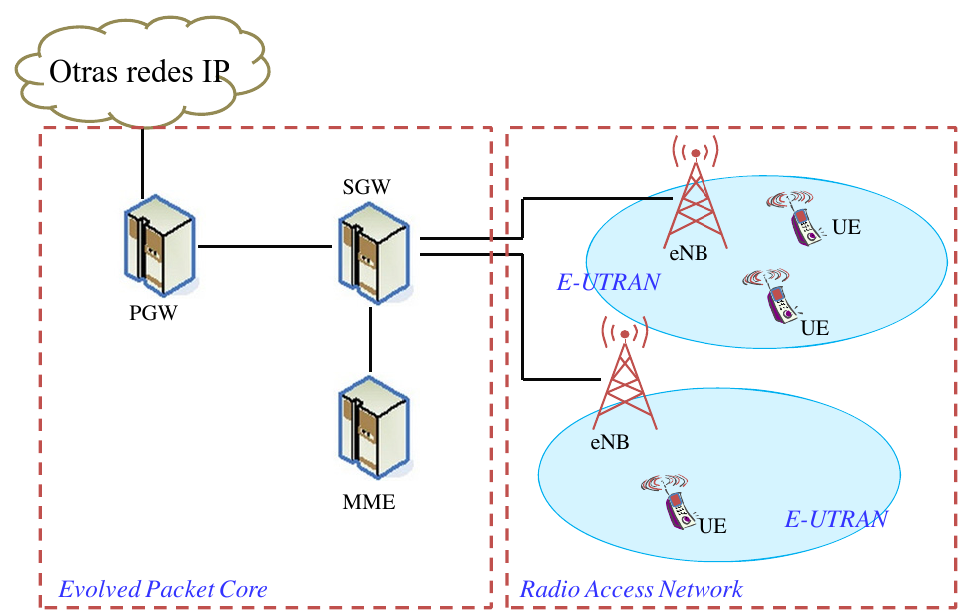
\includegraphics[scale=0.4]{imagenes/scheduling_italianos/scheduling_italianos-001_es.png}}
\end{figure}

\subsubsection{Protocolos e interfaces}

Para el correcto funcionamiento del sistema al completo, se establecen unos medios de comunicación entre elementos y unos métodos de funcionamiento \cite{RefWorks:81, RefWorks:26}.

Para la interconexión de las entidades funcionales a la par que su gestión independiente se definen interfaces genéricas.
Las interfaces son un medio de por el que se conectan dos entidades y su protocolo de funcionamiento.

\begin{figure}[H]
	\ffigbox[\FBwidth] {
	\caption[Interfaces de LTE]{Ejemplo de interfaces: Arquitectura simplificada de LTE.
	En LTE se define la interfaz X2 para conectar entidades eNB entre ellas y la interfaz S1 para conectar eNB con SGW.

	Fuente: \cite{RefWorks:81}}
	}
	{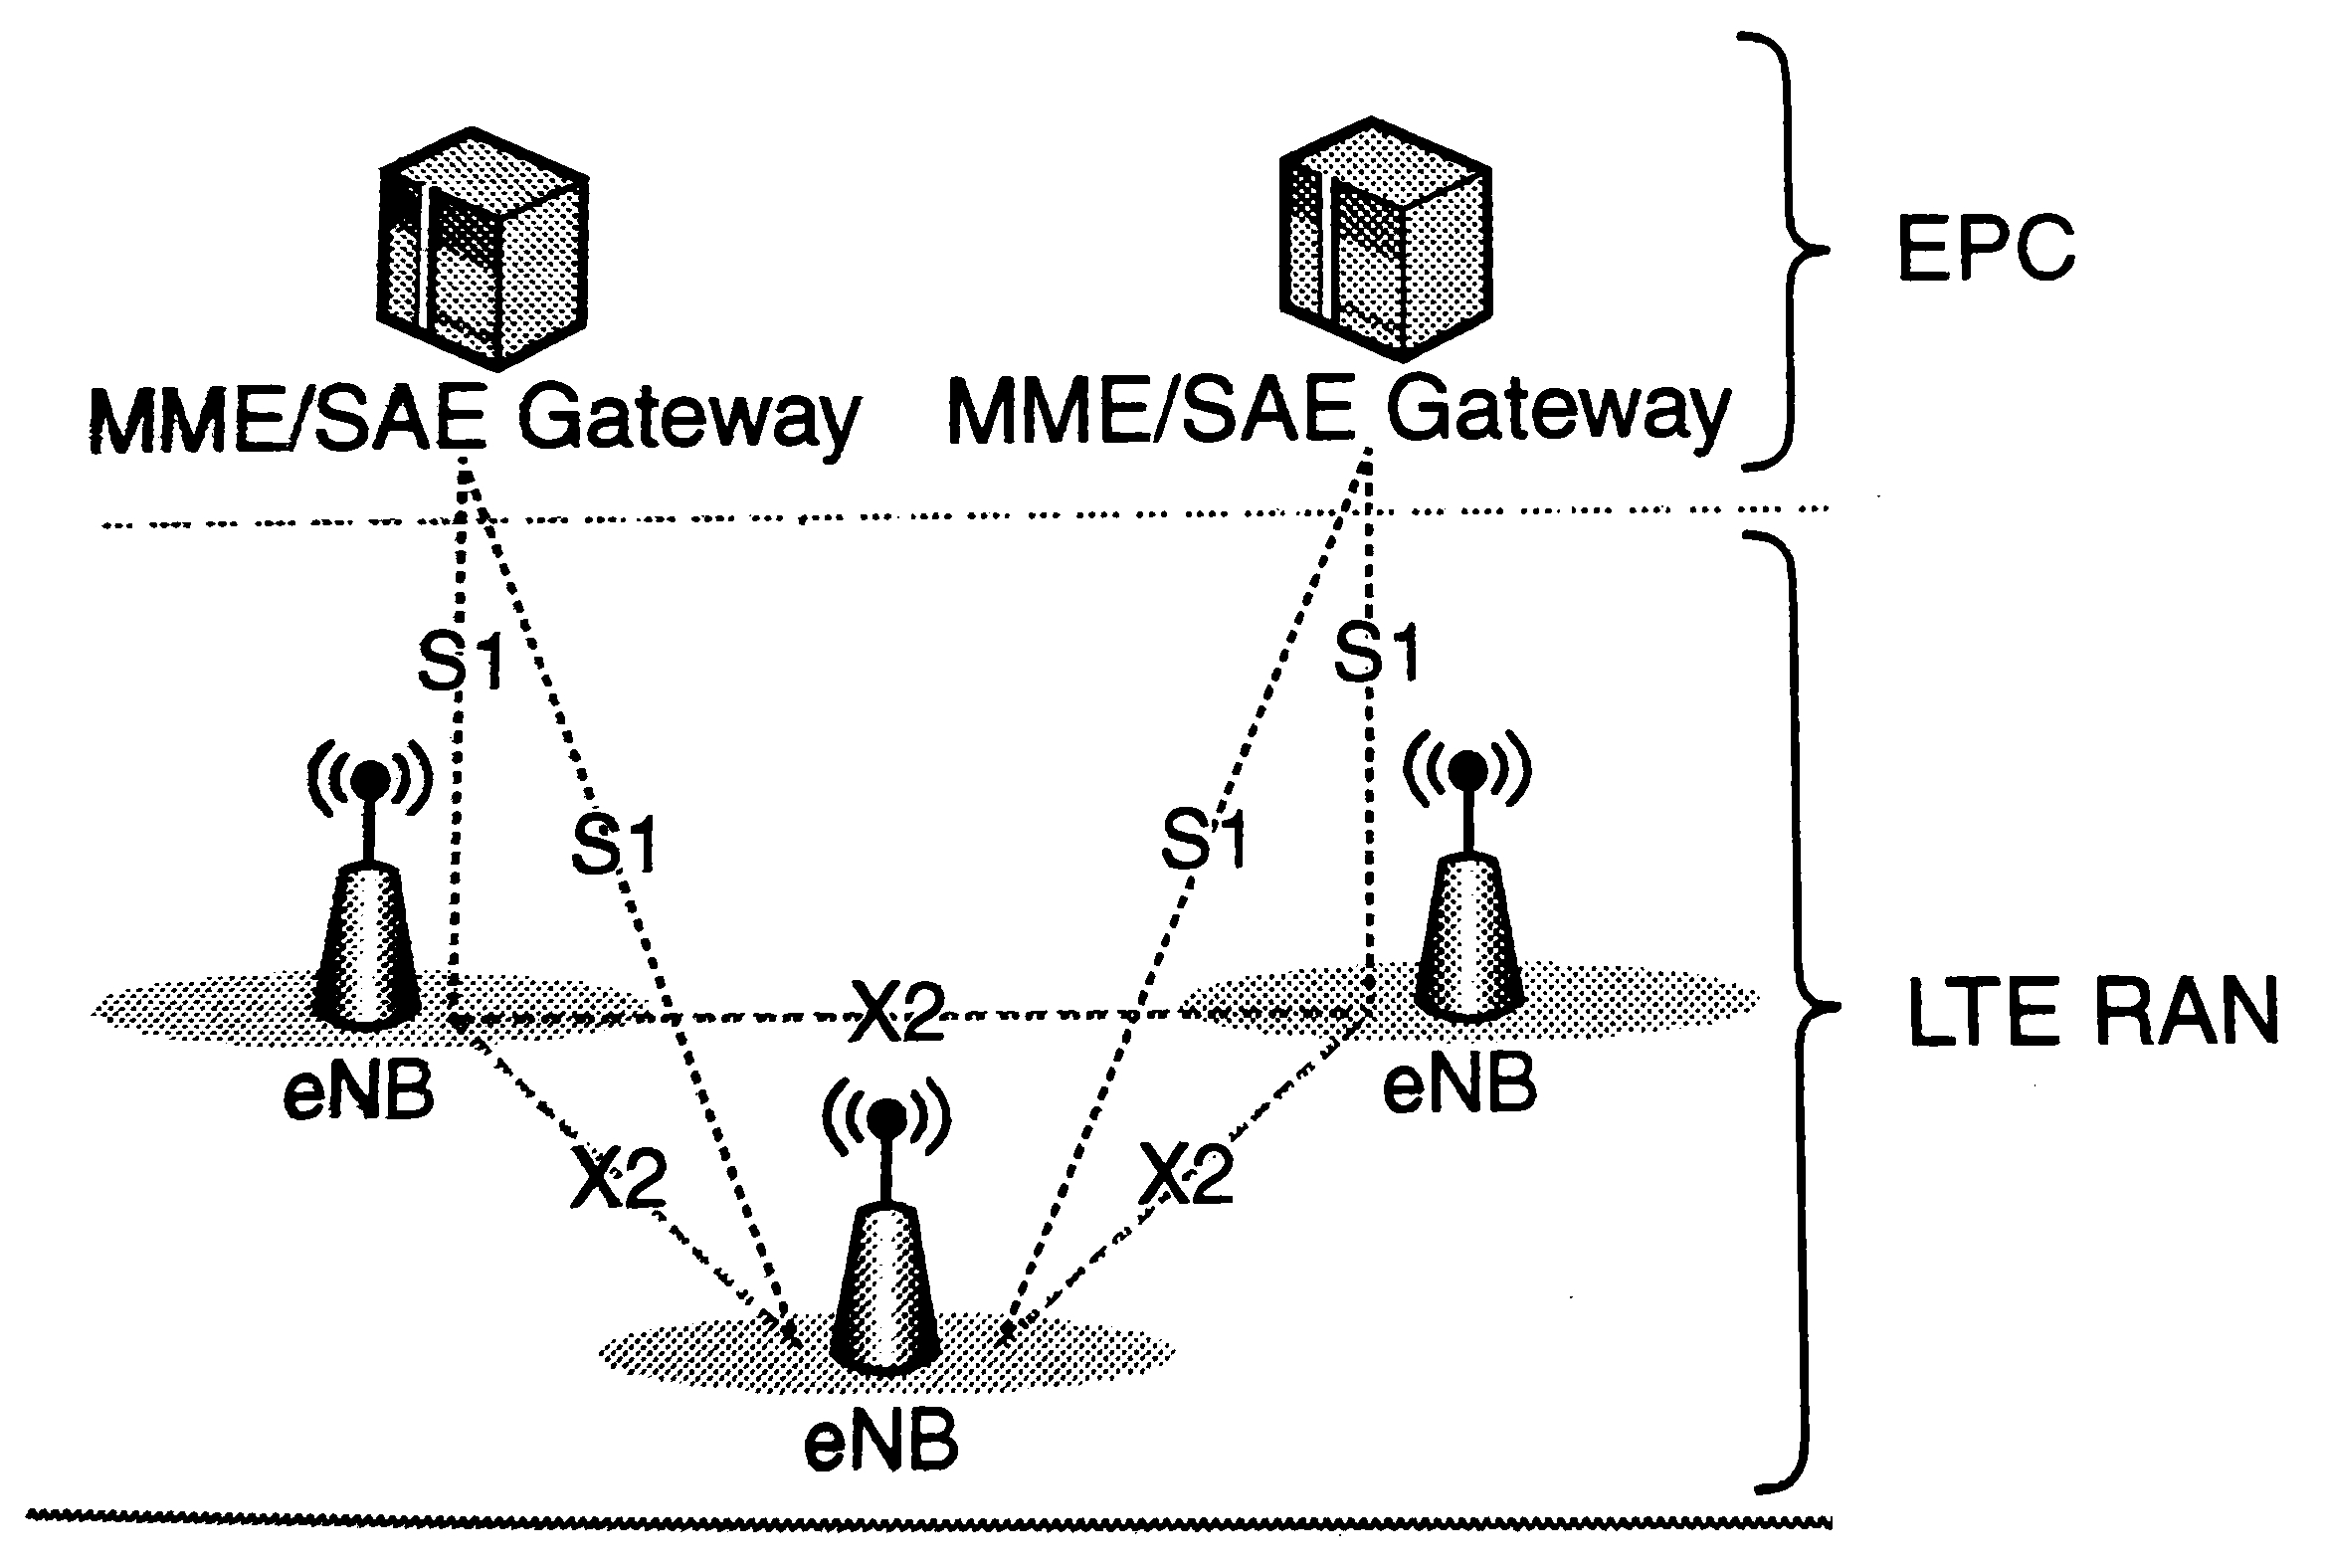
\includegraphics[scale=0.15]{imagenes/comunicaciones_moviles/cm_cap10_1_fixed.jpg}}
\end{figure}

Por otro lado, se definen una serie de protocolos que permiten interactuar entre los elementos de la red de manera ordenada e implementar las funciones de la red.
Estos protocolos hacen uso de las interfaces definidas.
Estos protocolos se diferencian por su lugar en la pila de protocolos.

La definición de los protocolos en los modernos sistemas de comunicaciones, especialmente para la RAN, incluye un complejo método de transmisión y señalización.
Este método es el uso de los denominados \textit{canales}:
\begin{itemize}
\item Canales lógicos: Están en la interfaz de la capa de acceso al medio y la capa de red.
Indican el tipo de información que ha de transmitirse.
\item Canales de transporte: Están en la interfaz de la capa de acceso al medio y la capa física.
Describen los formatos de transmisión.
\item Canales de físicos: Están en la capa física.
Especifican los recursos tiempo-frecuencia utilizados.
\end{itemize}
Para los canales, se define una manera de conexión y comunicación;
existe una correspondencia entre los canales físicos con los de transporte y otra entre los canales de transporte y los lógicos.
Así se define de manera cerrada y precisa la manera en la que interactúan las distintas entidades funcionales de la red.
A partir de LTE se define, además, un método análogo a los canáles en la capa física,
las denominadas \textit{señales}, que cumplen funciones complementarias a las de los canales.
En suma, a partir de los canales y las señales se implementan el resto de procolos de la red.

\begin{figure}[H]
	\ffigbox[\FBwidth] {
	\caption[Protocolos y canales de LTE]{Ejemplo de protocolos: Esquema de los niveles de la pila de protocolos, los canales y las señales de LTE.

	Fuente: \cite{RefWorks:81}}
	}
	{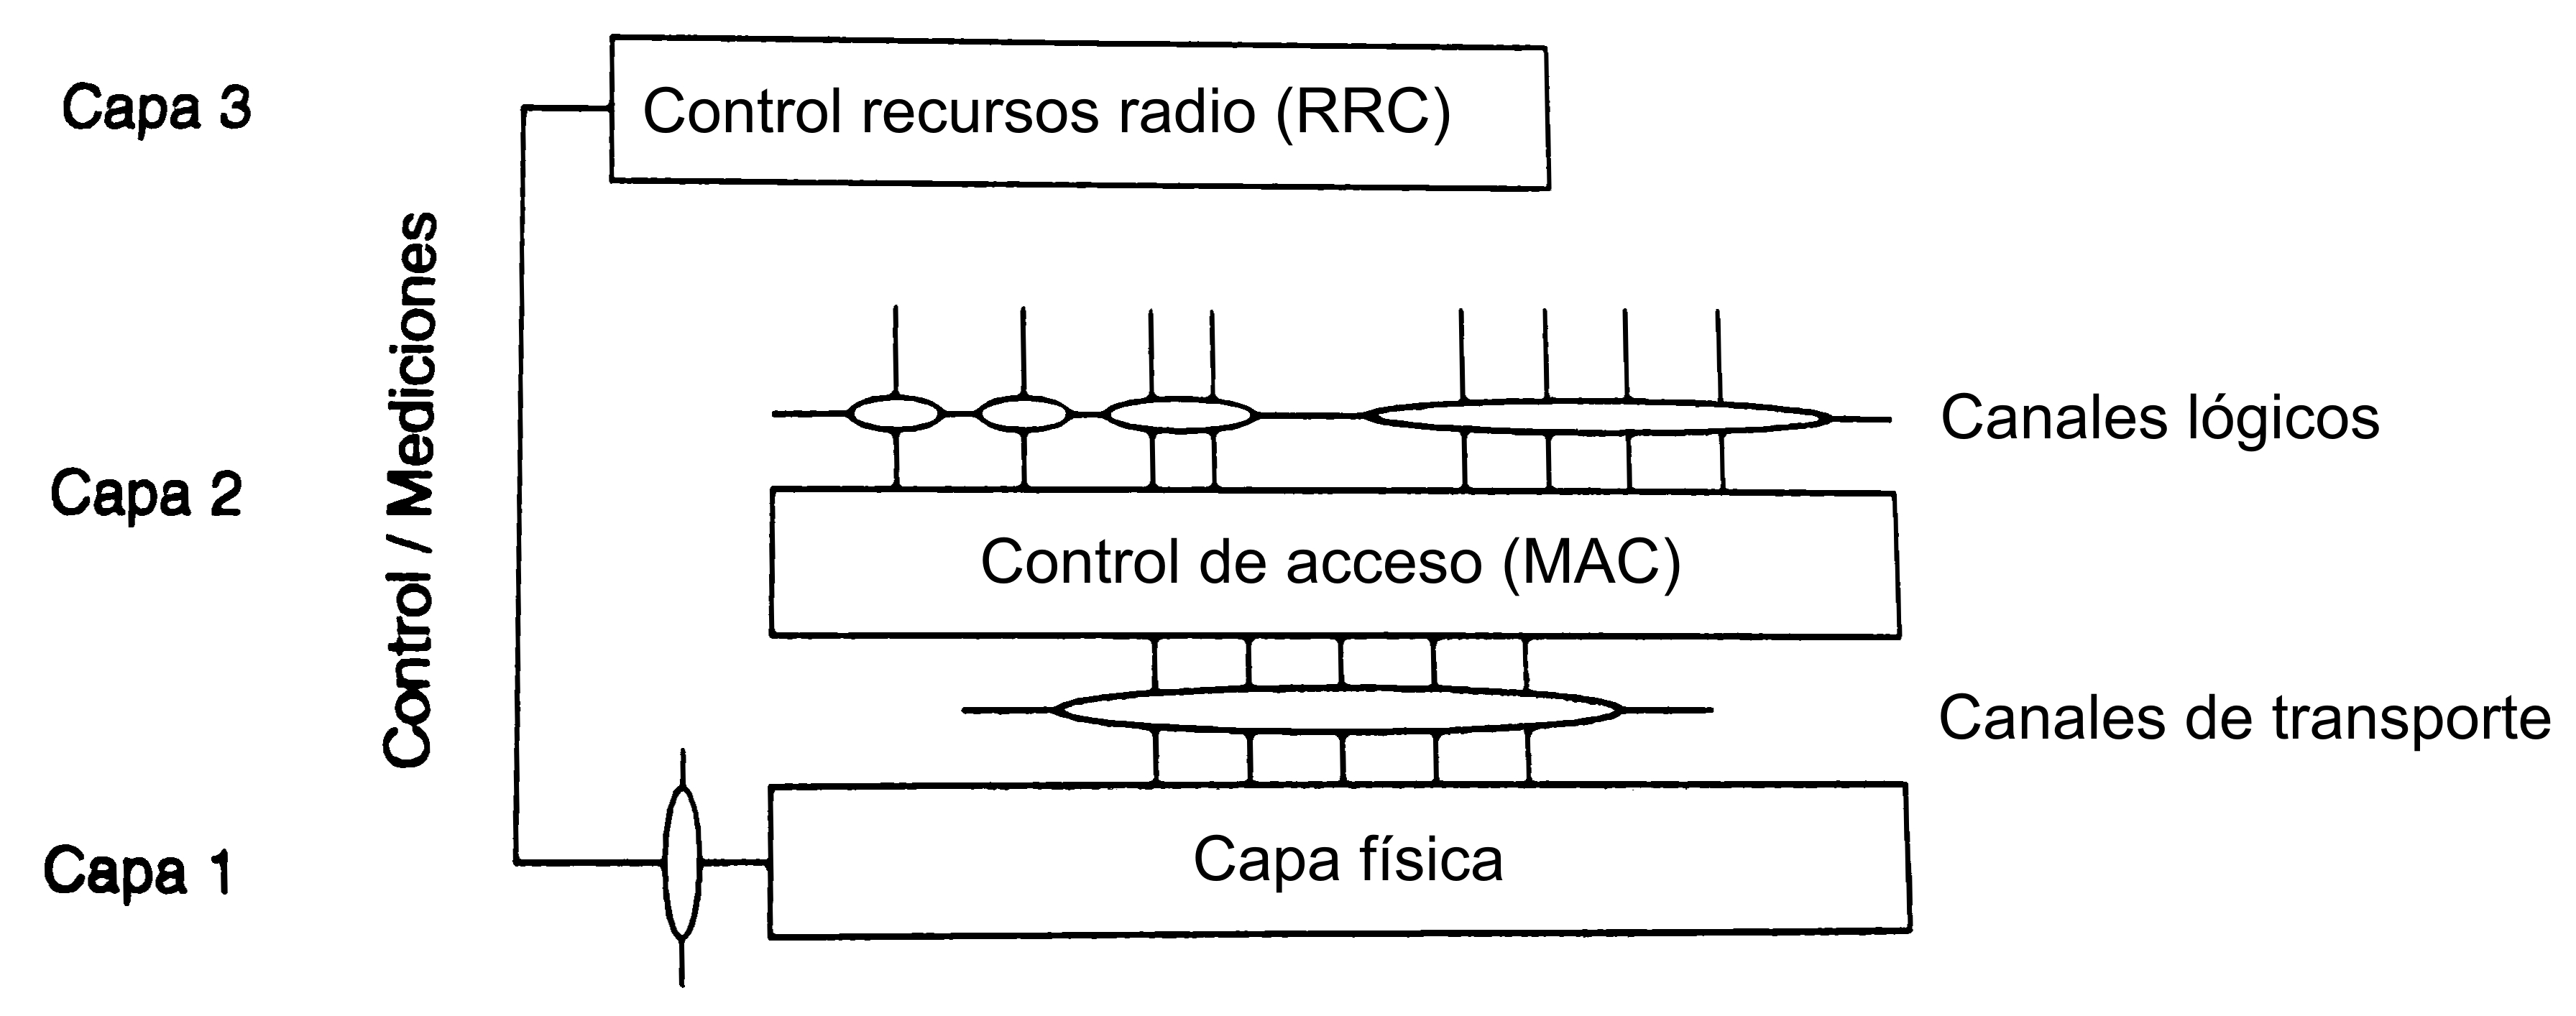
\includegraphics[scale=0.15]{imagenes/comunicaciones_moviles/cm_cap10_2_fixed.jpg}}
\end{figure}

\begin{figure}[H]
	\ffigbox[\FBwidth] {
	\caption[Correspondencia de canales de LTE en el enlace descendente]{Ejemplo de canales: Correspondencia entre los canales físicos y los de transporte en el enlace descendente para LTE.

	Fuente: \cite{RefWorks:81}}
	}
	{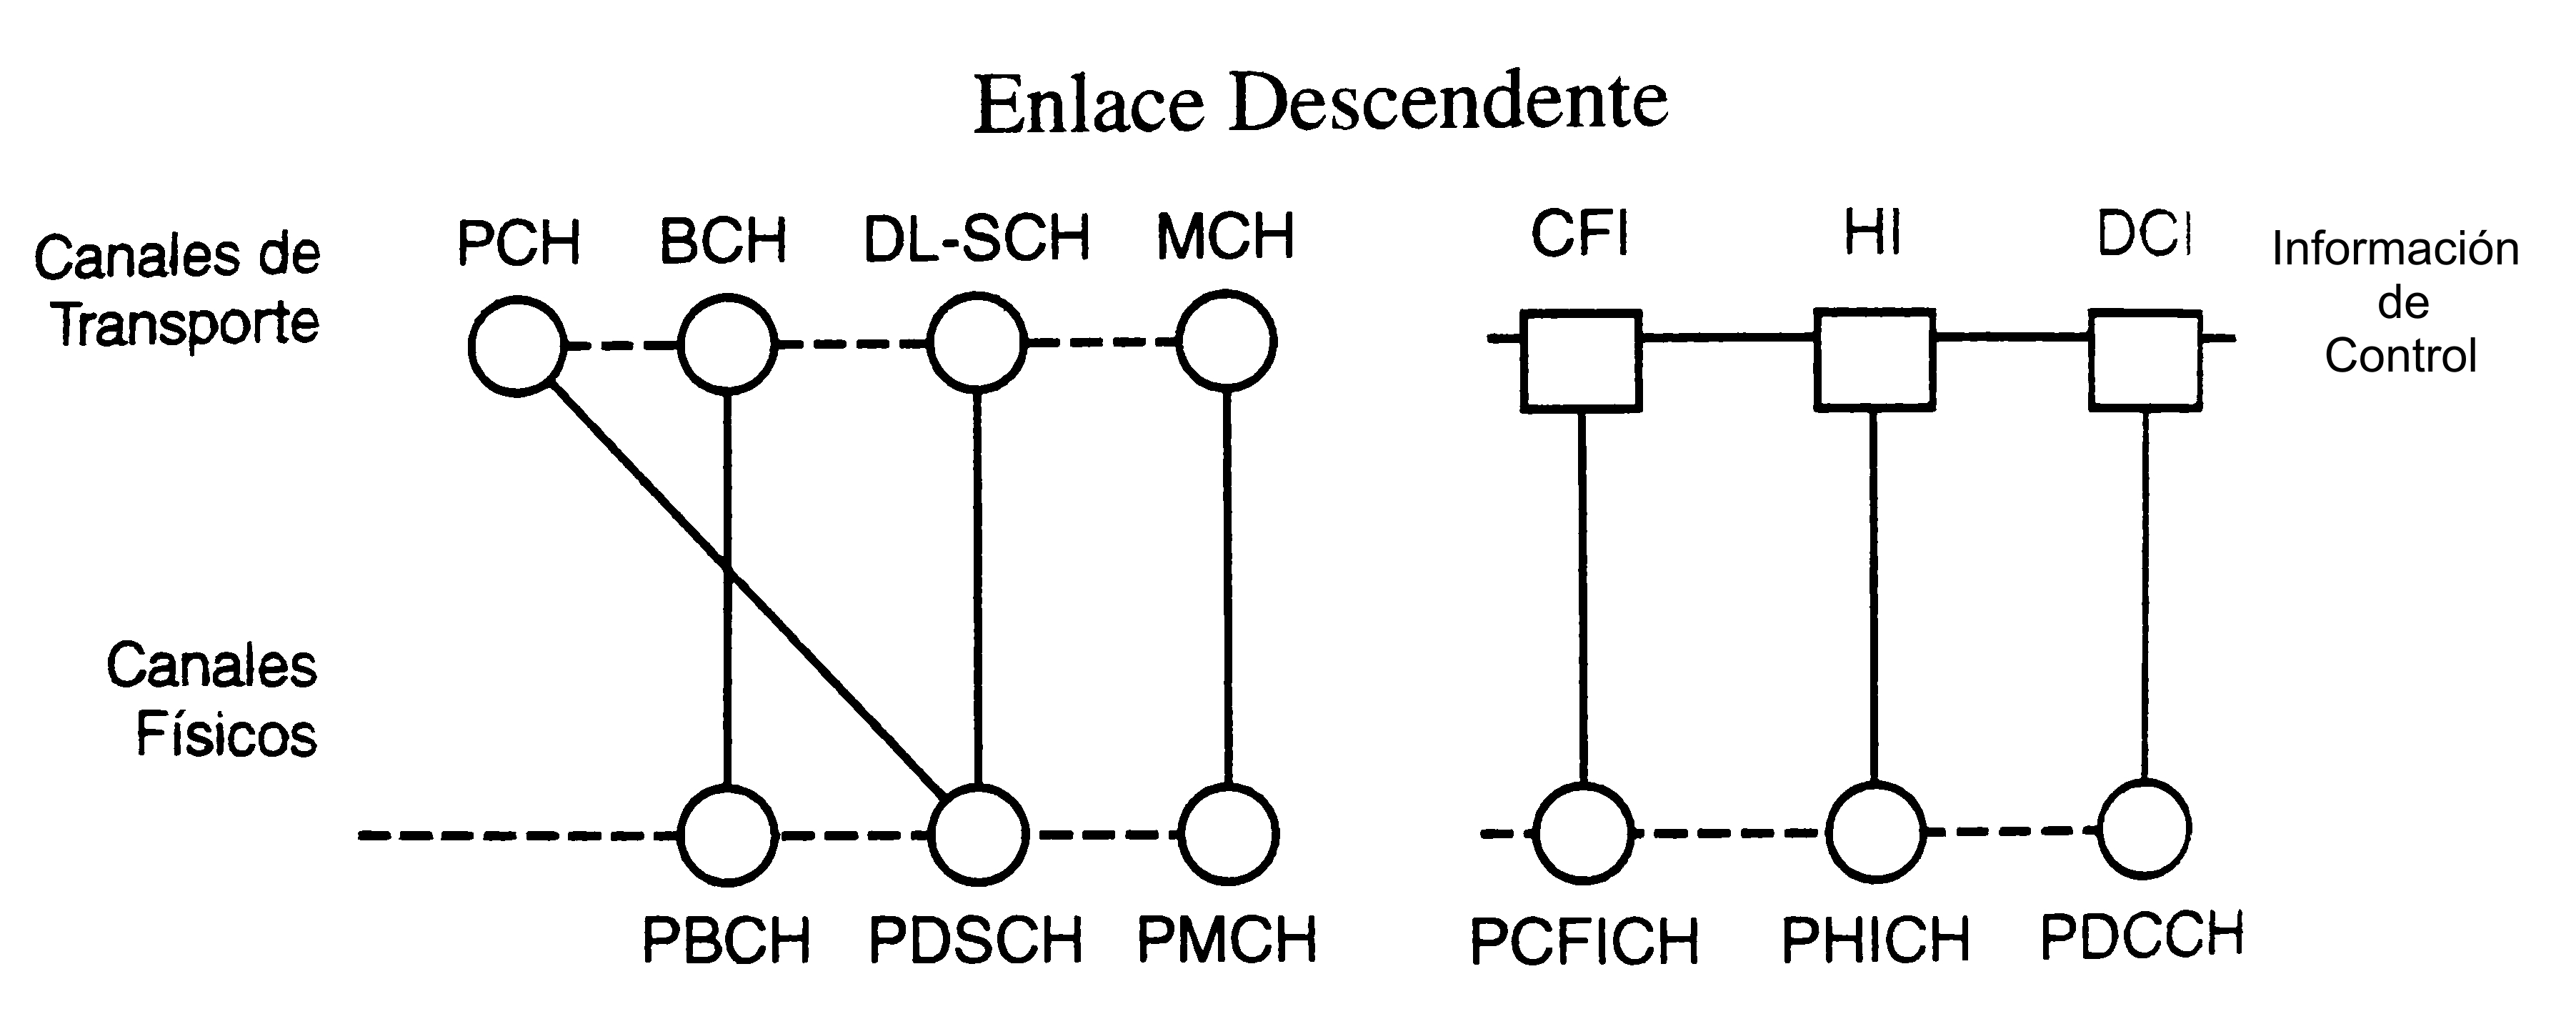
\includegraphics[scale=0.15]{imagenes/comunicaciones_moviles/cm_cap10_3_fixed.jpg}}
\end{figure}

\begin{figure}[H]
	\ffigbox[\FBwidth] {
	\caption[Protocolos y canales de la RAN de LTE]{Ejemplo de protocolos: Esquema de los protocolos de la RAN de LTE.
	Se puede ver los niveles de la pila de protocolos (PHY, MAC, RRC), los protocolos de cada nivel (AMC, HARQ, CQI, RLC), los canales lógicos (\textit{radio bearer}), los canales físicos (PDCCH, PDSCH, PUCCH, PUSCH) y las señales (PILOT).
	Los canales permiten implementar los protocolos.

	Fuente: \cite{RefWorks:26}}
	}
	{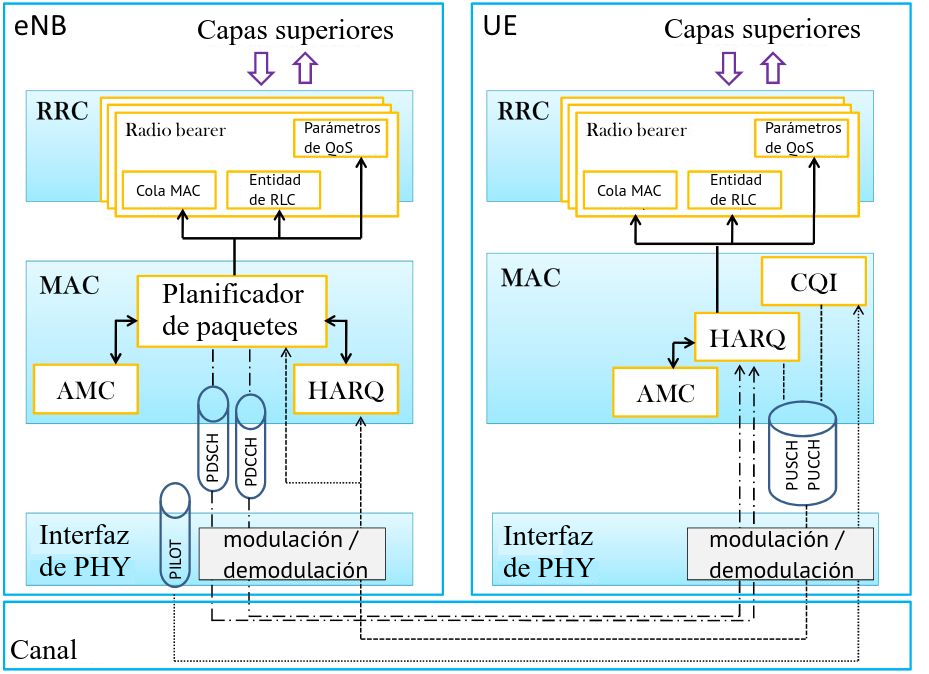
\includegraphics[scale=0.4]{imagenes/scheduling_italianos/scheduling_italianos-172_es.png}}
\end{figure}

\subsection{Transmisión inalámbrica}

\subsubsection{Transmisión en el enlace radioeléctrico}

El espacio libre es el canal de la interfaz de radio; este canal somete a la señal de radiofrecuencia que se transmite a diversos efectos.
Los componentes físicos del sistema de comunicaciones, como antenas y amplificadores, también producen efectos apreciables en la señal transmitida.
En suma, se cuentan los siguientes efectos:

\begin{itemize}
	\item Ruido \cite{RefWorks:78}: Es una señal aleatoria que se suma a la transmitida.
	Es generada por el canal, por los amplificadores de radiofrecuencia y otros componentes electrónicos.
	$$P_{rx} = P_{tx} + P_{N}$$
	Para su manejo en sistemas digitales, es necesario que la relación entre la potencia media de la señal ($P_{tx}$) y la potencia de ruido ($P_{N}$), denominada relación portadora a ruido ($\frac{C}{N}$), supere un umbral denominado ``relación de protección'' ($R_p$):
	$$\frac{C}{N} = \frac{P_{tx}}{P_{N}} \rightarrow \left( \frac{C}{N} \right)_{dB} = 10 \log P_{tx} - 10 \log P_{N} > R_p$$
	\item Interferencia \cite{RefWorks:78}: Es una señal usada por otro sistema de comunicaciones que utiliza los mismos recursos de tiempo-frecuencia.
	Se suma a la seña transmitida.
	$$P_{rx} = P_{tx} + P_{I}$$
	Para su manejo en sistemas digitales, es necesario que la relación entre la potencia media de la señal ($P_{tx}$) y la potencia de ruido ($P_{I}$), denominada relación portadora a interferencia ($\frac{C}{I}$), supere un umbral denominado ``relación de protección'' ($R_p$):
	$$\frac{C}{I} = \frac{P_{tx}}{P_{I}} \rightarrow \left( \frac{C}{I} \right)_{dB} = 10 \log P_{tx} - 10 \log P_{I} > R_p$$
	\item Pérdida por propagación (atenuación) \cite{RefWorks:79}: Es la degradación de la señal al transmitirse por el medio de propagación.
	El valor mediano de la pérdida es función de la distancia entre el transmisor y el receptor.
	La mayoría de los modelos propuestos predice una variación según una ley potencial de la forma:
	$$l_b = l_{att} (d) = k \cdot d^n \rightarrow L_b = L_{att} (d) = 10 \log (k) +10 n \log (d)$$
	\item Desvanecimiento por sombra (\textit{shadow fading}) \cite{RefWorks:79}: Es la degradación de la señal debida a la influencia del terreno entre el transmisor y el receptor.
	Produce una atenuación variable en torno al promedio pronosticado por la pérdida por propagación y dependiente del lugar físico en el que se encuentra el transmisor ($x$, $y$).
	Se ha llegado a la conclusión de que esta función puede modelarse mediante una variable aleatoria gaussiana si se expresa la pérdida en decibelios, o log-normal, si se expresa en unidades naturales:
	$$L_b = L_{att} (d) + L_{sf} (x, y)$$
	$$L_{sf} (x, y) \sim \operatorname{\mathcal{N}} (\mu, \sigma)$$
	De manera usual, pero no de manera estricta, se puede atribuir el desvanecimiento lento (\textit{slow fading}), es decir, las variaciones lentas del canal, al desvanecimiento por sombra;
	el desvanecimiento lento también recibe contribuciones del multitrayecto.
	\item Desvanecimiento por multitrayecto (\textit{multipath fading}) \cite{RefWorks:79}: Es la degradación de la señal debida a la presencia de obstáculos próximos al móvil.
	Se incluye en el modelo de la pérdida básica de propagación un factor de desvanecimiento multitrayecto que depende de la distancia ($s$) (o del tiempo, $t$, para una velocidad del receptor conocida, $v$, o simplemente del tiempo debido a la modificación de los obstáculos) y de la frecuencia ($f$).
	El factor es una variable aleatoria cuyo efecto sobre la envolvente de la señal recibida se describe habitualmente mediante una distribución Rayleigh:
	$$L_b = L_{att} (d) + L_{sf} (x, y) + L_{ff} (t, f) $$
	$$\operatorname{P} \left( L_{ff} (t, f) = r \right) = \frac{r}{b} \exp \left( \frac{-r^2}{2 b} \right), b = \frac{\bar{r^2}}{2}$$
	En general, sí se puede atribuir el desvanecimiento rápido (\textit{fast fading}), es decir, las variaciones rápidas del canal, al desvanecimiento por multitrayecto.
	\begin{figure}[H]
		\ffigbox[\FBwidth] {
		\caption[Desvanecimiento rápido]{Ilustración del desvanecimiento rápido: Pérdidas debida al desvanecimiento rápido en el dominio tiempo-frecuencia.

		Fuente: \cite{RefWorks:26}}
		}
		{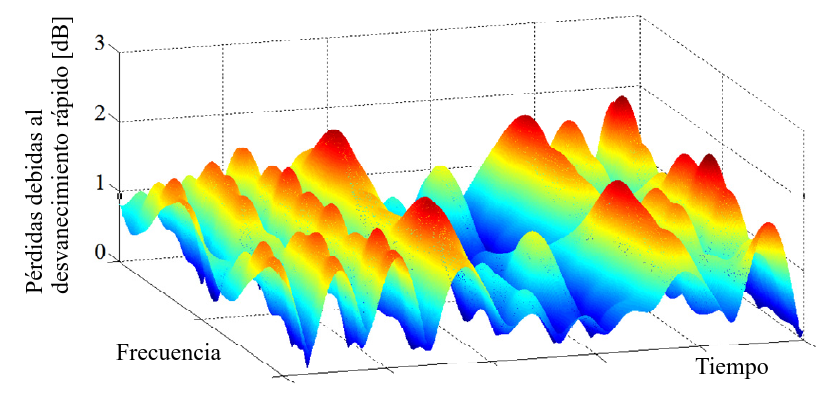
\includegraphics[scale=0.6]{imagenes/scheduling_italianos/scheduling_italianos-174_es.png}}
	\end{figure}
\end{itemize}

\begin{figure}[H]
	\ffigbox[\FBwidth] {
	\caption[Atenuación de la señal]{Ejemplo de degradación de la señal: Variación en función del tiempo de la envolvente de una señal multitrayecto de frecuencia 900 MHz, para un determinado desplazamiento del receptor móvil.

	\textbf{Desvanecimiento rápido}: Se observan claramente las rápidas e intensas fluctuaciones del nivel, así como su relativa regularidad.
	Los mínimos de amplitud vienen a estar separados entre sí por distancias  múltiplos de semilongitudes de onda de la señal transmitida.

	\textbf{Desvanecimiento lento}: Cuando el receptor realiza un recorrido más largo, van cambiando los factores que intervienen en la propagación y se observa que sigue habiendo fluctuaciones, pero con una media que varía más lentamente.
	Al promedio de la señal en un pequeño tiempo o recorrido se le llama media local.
	Se observa la variación de la media local con el tiempo, que se describe por la función $L_{sf} (x, y)$.

	Fuente: \cite{RefWorks:79}}
	}
	{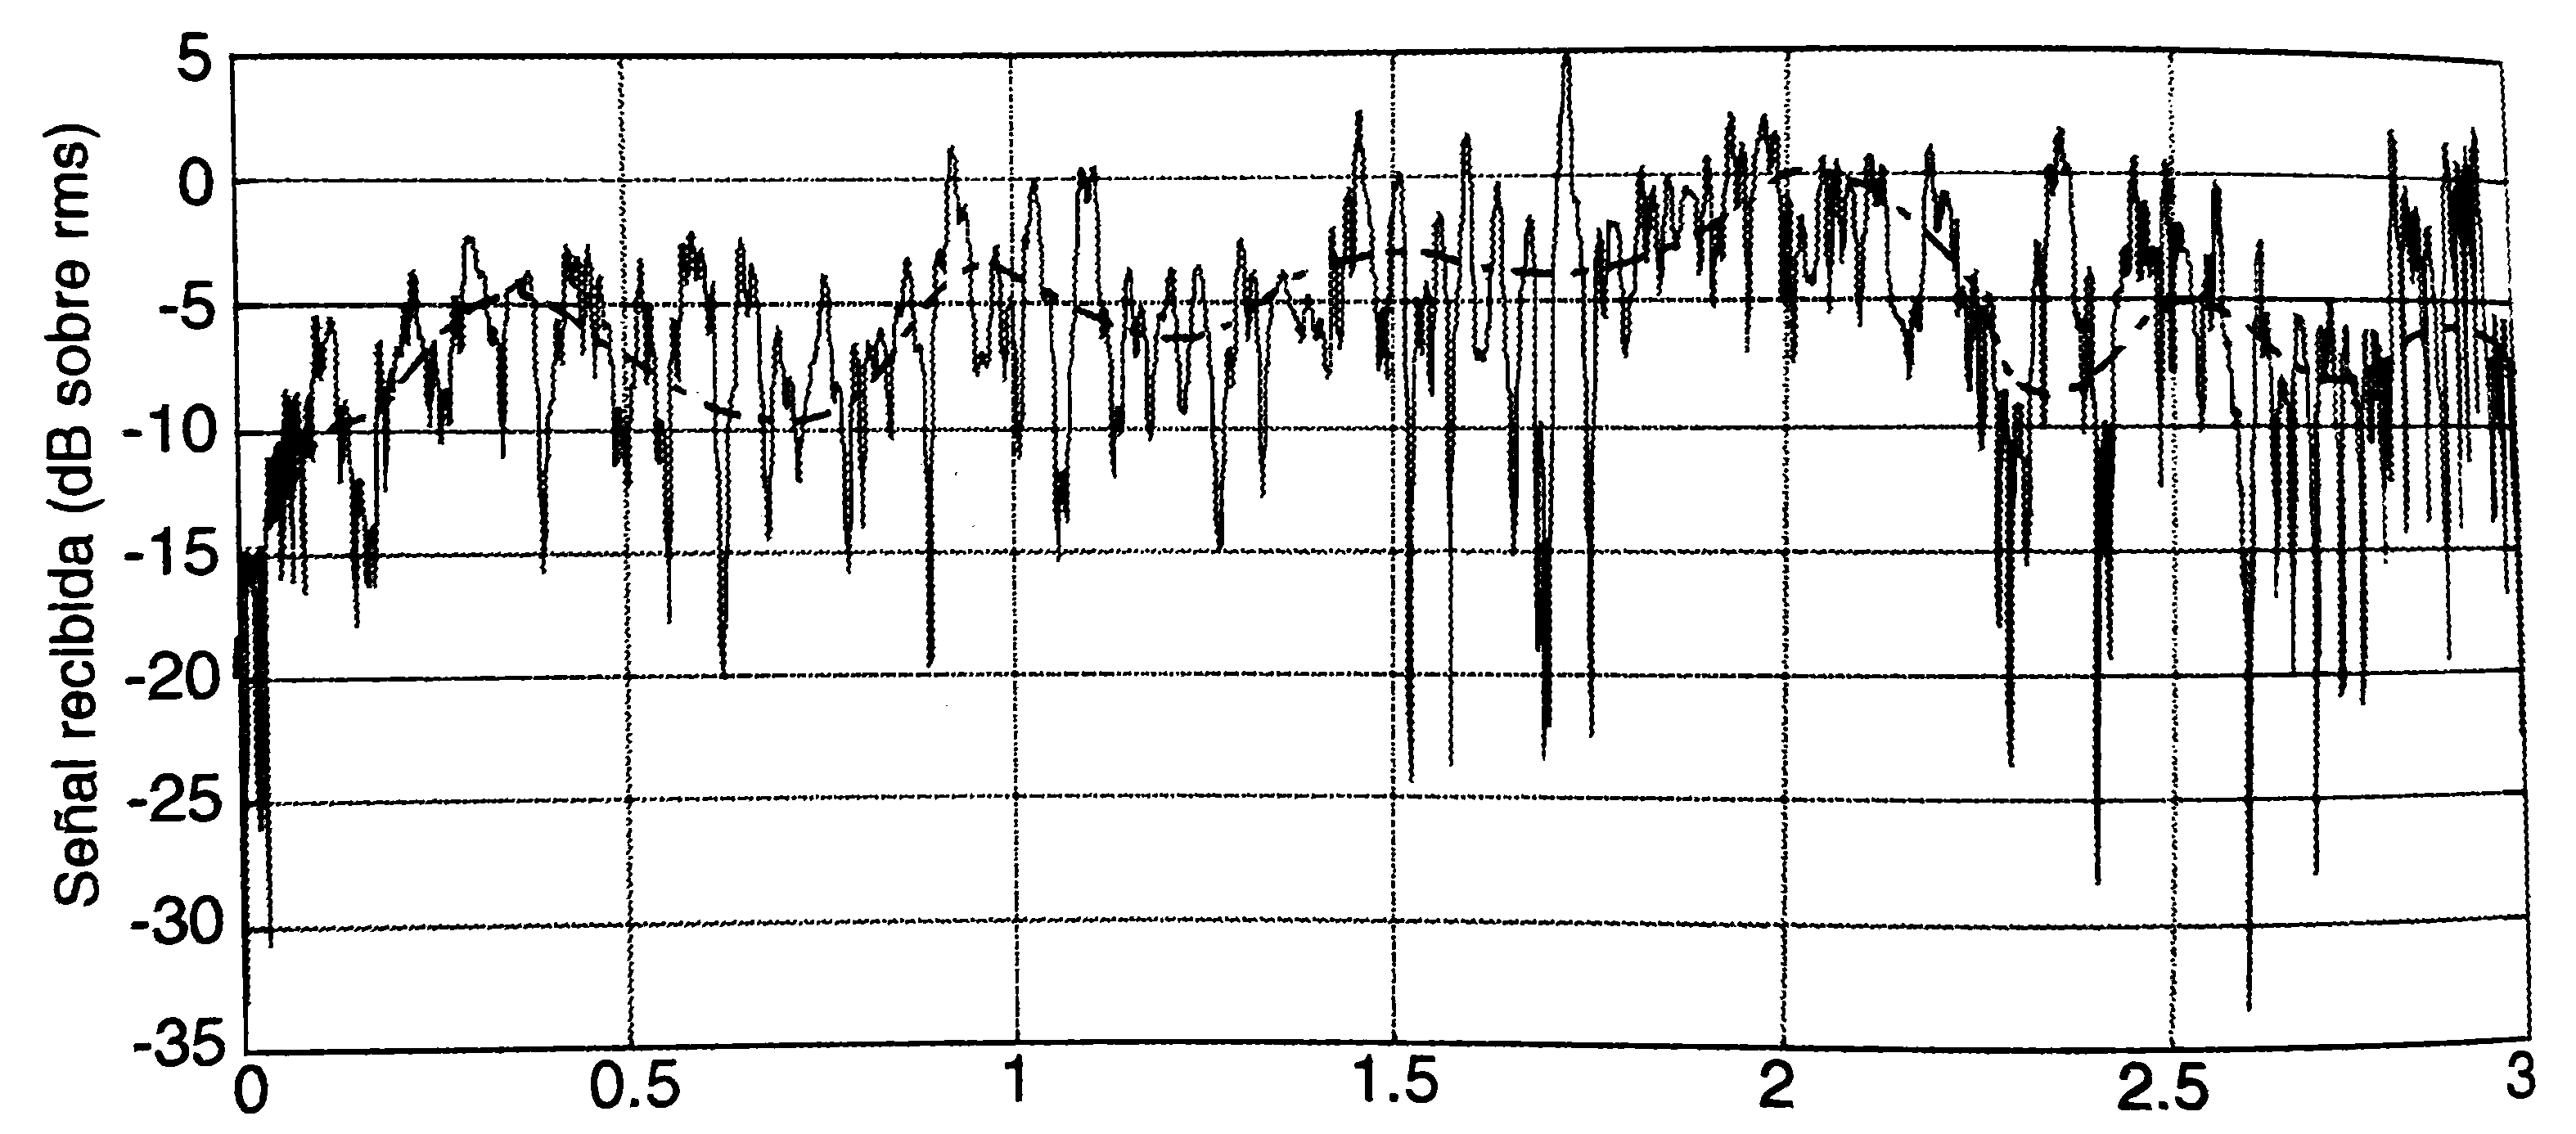
\includegraphics[scale=0.15]{imagenes/comunicaciones_moviles/cm_cap3_2_fixed.jpg}}
\end{figure}

\subsubsection{Análisis del enlace radioeléctrico}

Los efectos sobre la señal transmitida se estudian a través de dos abstracciones del sistema de comunicaciones: el balance de enlace \cite{RefWorks:78} y los modelos de canal \cite{RefWorks:79}.

\paragraph{Balance de enlace}

En el análisis y proyecto de los sistemas de comunicaciones es necesario preparar balances de pérdidas y ganancias de potencias y realizar cálculos de niveles en diferentes puntos.
El balance del enlace es la relación que expresa la potencia disponible en función de la potencia entregada por el transmisor y las diferentes pérdidas y ganancias que aparecen en el trayecto entre ambos.

\begin{figure}[H]
	\ffigbox[\FBwidth] {
	\caption[Modelo energético]{Ejemplo de balance de enlace: Modelo energético de un sistema de comunicaciones.
	Muestra el paso de la señal desde el terminal del transmisor hasta el terminal del receptor.
	Este modelo permite el cálculo del balance de enlace.

	Fuente: \cite{RefWorks:78}}
	}
	{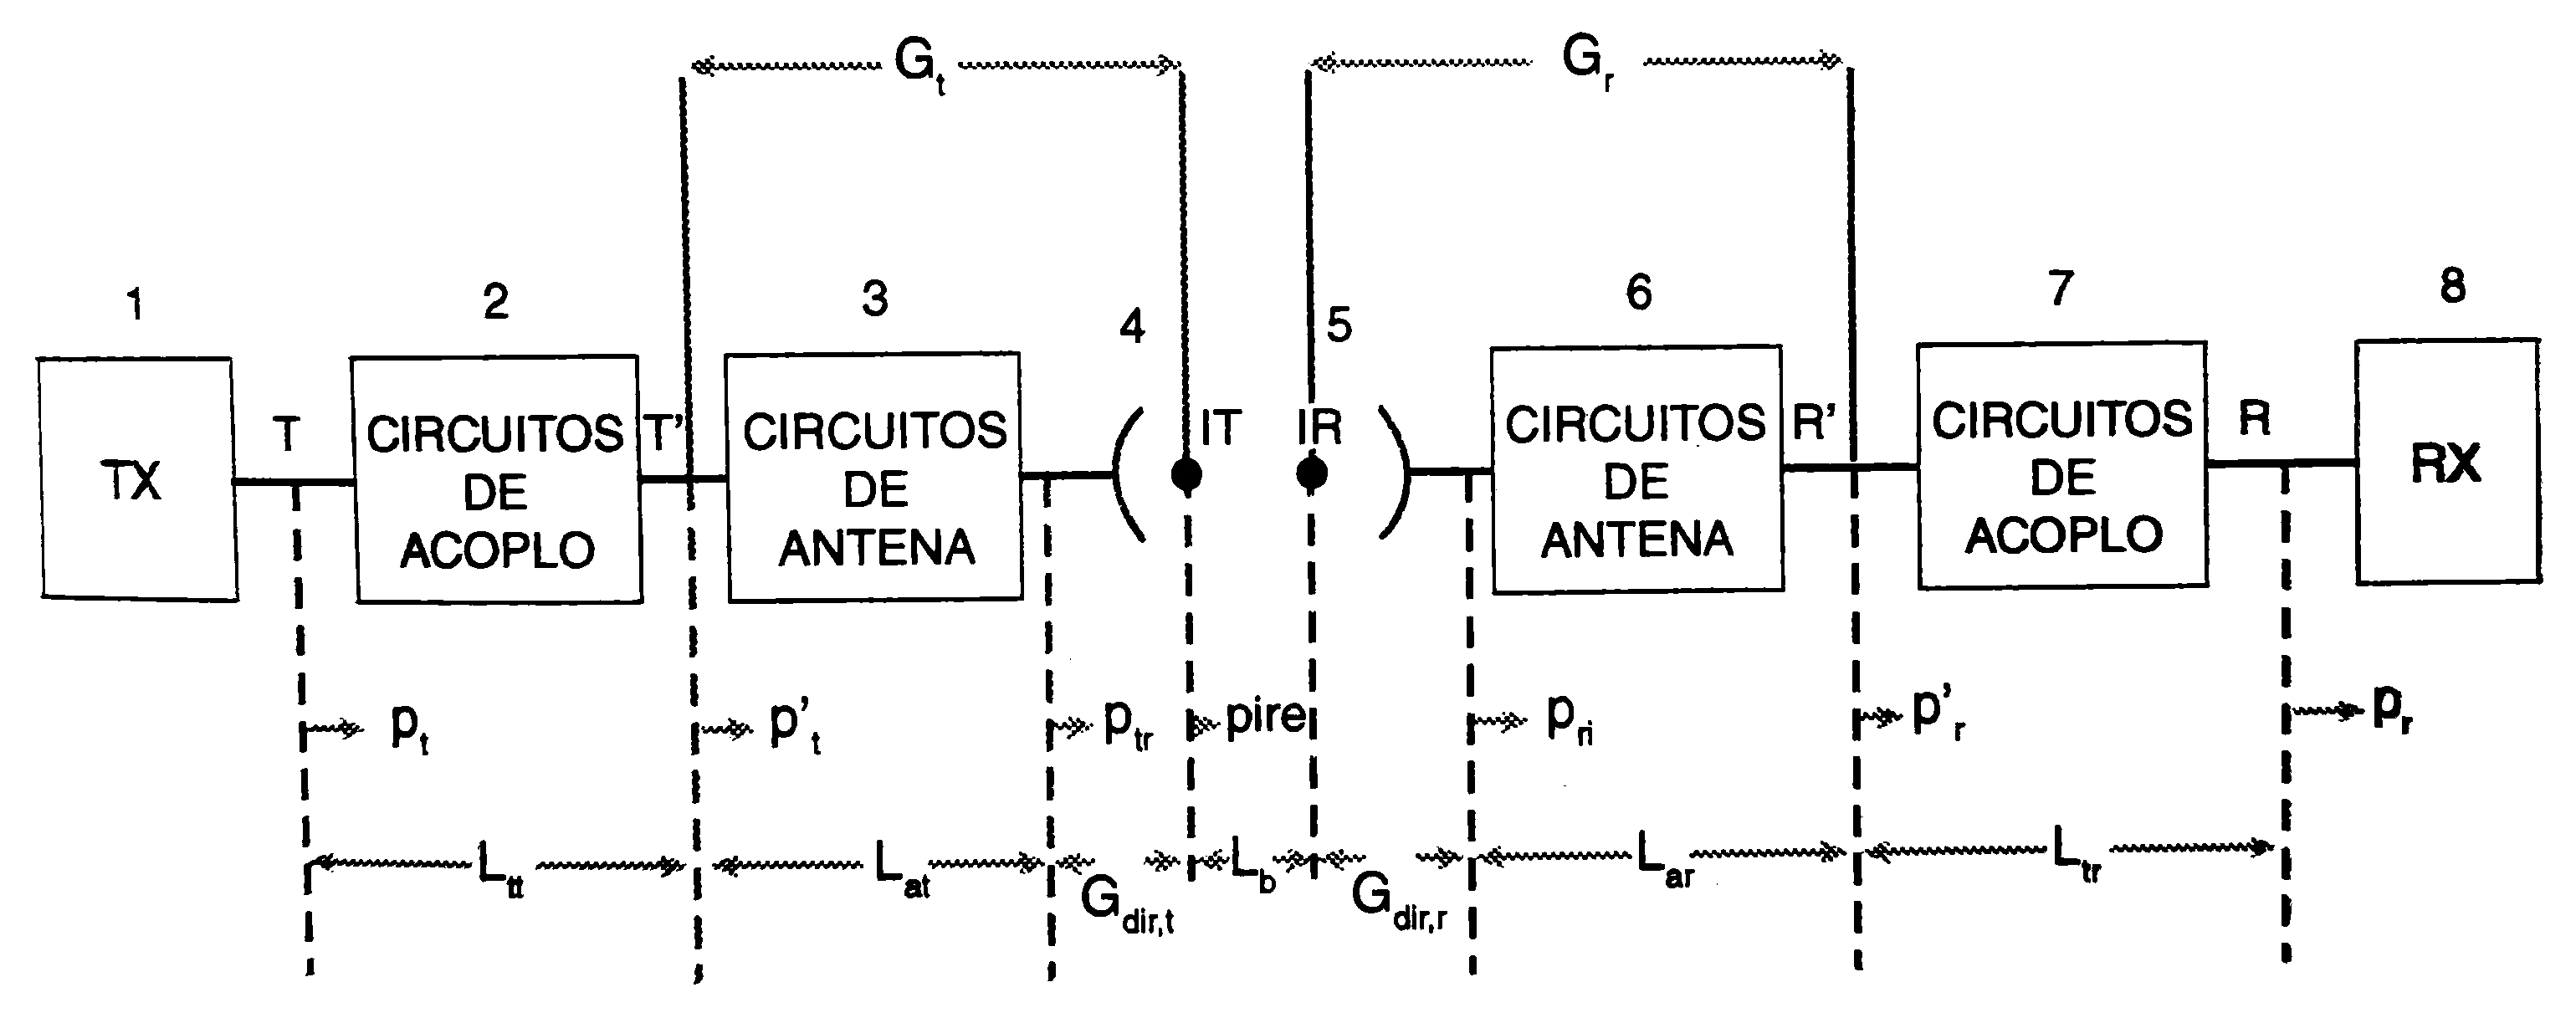
\includegraphics[scale=0.15]{imagenes/comunicaciones_moviles/cm_cap2_5_fixed.jpg}}
\end{figure}

%Las pérdidas reciben contribuciones como las descritas en el apartado anterior y otras debidas a los componentes físicos del sistema,
%mientras que las ganancias son proporcionadas por los elementos activos del enlace.
%Para expresar un balance de enlace es necesario tener conocimiento de cada componente del sistema de comunicaciones que atraviesa la señal transmitida.
%La ecuación general de balance del enlace es:
%$$P_r = P_t - L_{tt} + G_t - L_b + G_r - L_{tr}$$
%Donde:
%\begin{itemize}
%	\item $P_r$ es la potencia en el receptor.
%	\item $P_t$ es la potencia en el transmisor.
%	\item $L_{tt}$ son las pérdidas en los circuitos de acoplo del transmisor.
%	\item $G_t$ es la gancia de potencia en la antena del transmisor.
%	\item $L_b$ son las pérdidas básicas de propagación.
%	\item $G_r$ es la gancia de potencia en la antena del receptor.
%	\item $L_{tr}$ son las pérdidas en los circuitos de acoplo del receptor.
%\end{itemize}

\paragraph{Modelos de canal}

%En la propagación por canales móviles deben destacarse tres aspectos fundamentales, que son:
%
%\begin{itemize}
%	\item La cobertura zonal, lo que implica la necesidad de realizar predicciones  de propagación entre el transmisor y un elevado número de puntos del área de cobertura.
%	\item La multiplicidad de trayectos entre el transmisor y un receptor situado en un punto determinado.
%	\item La variabilidad de de los trayectos, debida al desplazamiento de los terminales móviles,
%	lo que supone una variación con la distancia y con el tiempo de las condiciones de propagación y, en consecuencia, del nivel y la forma de onda de la señal recibida.
%\end{itemize}

Como se vio en el apartado anterior, la señal transmitida es afectada de múltiples maneras.
Es por ello que la planificación y proyecto de los modernos sistemas de radiocomunicaciones móviles exige la realización de cuatro actividades relacionadas con la propagación:
\begin{itemize}
	\item Caracterización del canal móvil en banda estrecha.
	\item Caracterización del canal móvil en banda ancha.
	\item Desarrollo de modelos de simulación.
	\item Realización de medidas radioeléctricas.
\end{itemize}

Es por esto que el desarrollo de modelos matemáticos capaces de predecir la alteración de la señal transmitida es fundamental.
De la misma manera, estos modelos se pueden aplicar en simuladores que aumenten la precisión de la predicción.

\subsection{Sistema celular}

Las redes móviles, a diferencia de otros sistemas de comunicaciones inalámbricas, presentan un diseño de \textit{celdas} o \textit{células} que dividen el espacio físico en zonas de cobertura, cada una de ellas dotada de una estación base.
Además, las celdas se agrupan en los denominados clústeres, en cada uno de los cuales se utiliza el mismo conjunto de frecuencias para la transmisión;
el reparto apropiado de las frecuencias entre las celdas, cada una con su frecuencia y evitando que linden dos celdas con la misma frecuencia, previene las interferencias.
También es posible dividir la celda en sectores, cada uno atendido por una antena que radia con una frecuencia distinta desde el mismo lugar físico, en el que se encuentra la estación base.
Estos métodos se denominan \textit{reutilización de frecuencias} \cite{RefWorks:91}.

\begin{figure}[H]
% 	{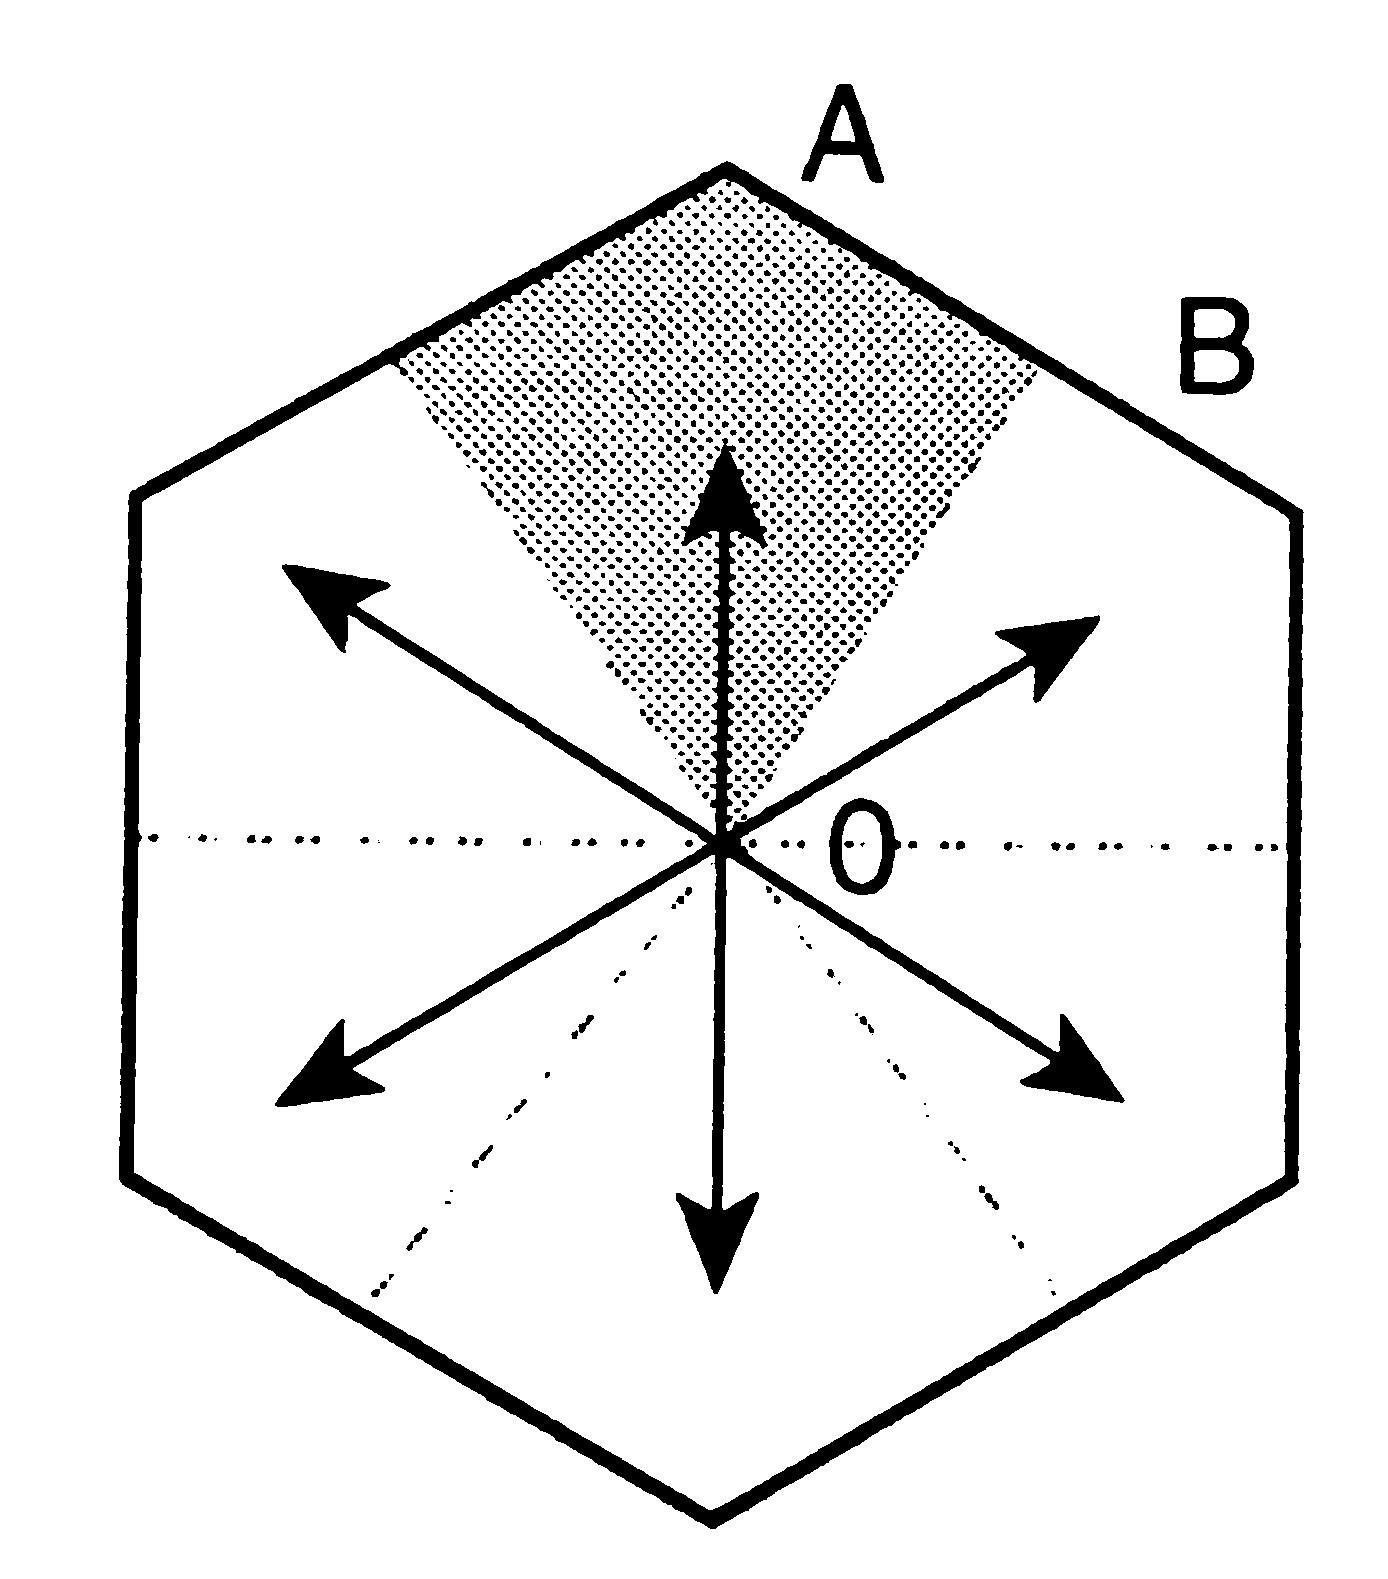
\includegraphics[scale=0.1]{imagenes/comunicaciones_moviles/cm_cap4_6_fixed.jpg}}
	\ffigbox[\FBwidth] {
	\caption[Clústeres]{Ejemplo de sistema celular: Esquema de un sistema celular de segunda generación.

	(Izquierda): Se pueden ver los sectores en la celda.

	(Derecha): Se pueden ver las celdas y un clúster de celdas.

	Fuente: \cite{RefWorks:91}}
	}
	{
\includegraphics[scale=0.1]{imagenes/comunicaciones_moviles/cm_cap4_6_fixed_long.jpg}
	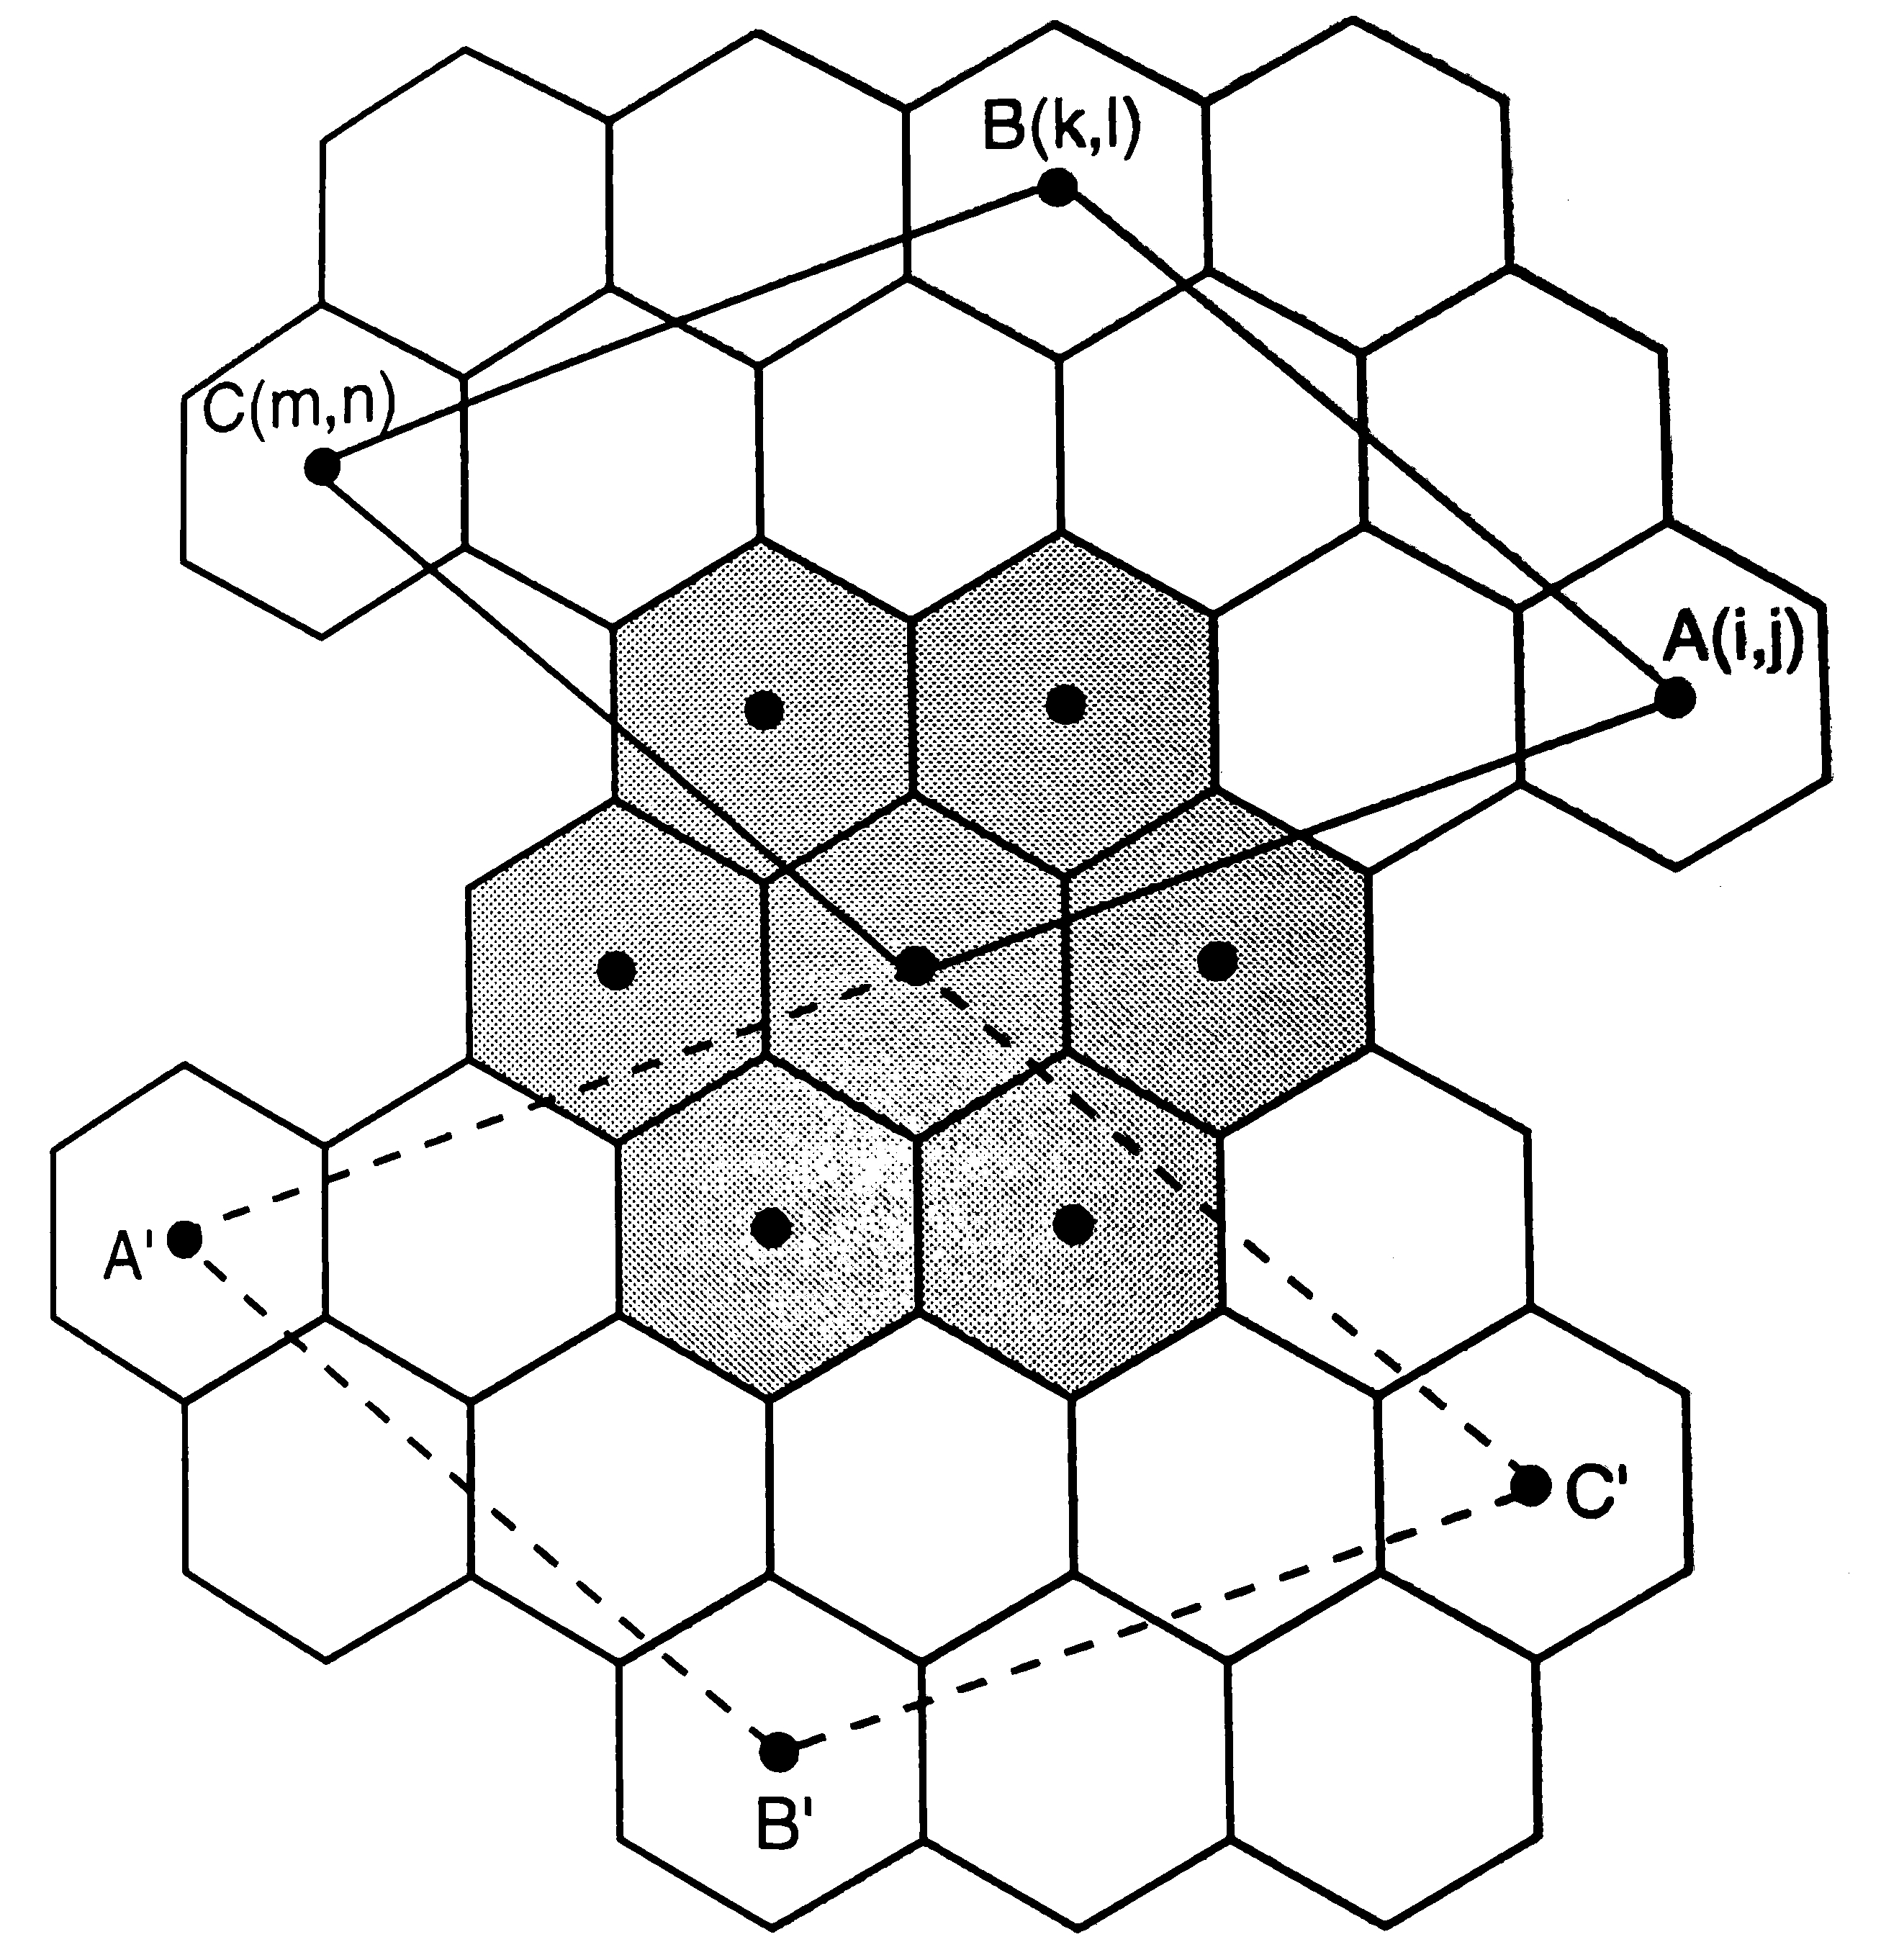
\includegraphics[scale=0.15]{imagenes/comunicaciones_moviles/cm_cap4_9_fixed.jpg}}
\end{figure}

%\begin{figure}[H]
%	\ffigbox[\FBwidth] {
%	\caption[Sectores]{Ejemplo de sistema celular: Esquema de un sistema celular de segunda generación.
%	Se pueden ver los sectores en la celda.
%
%	Fuente: \cite{RefWorks:91}}
%	}
%	{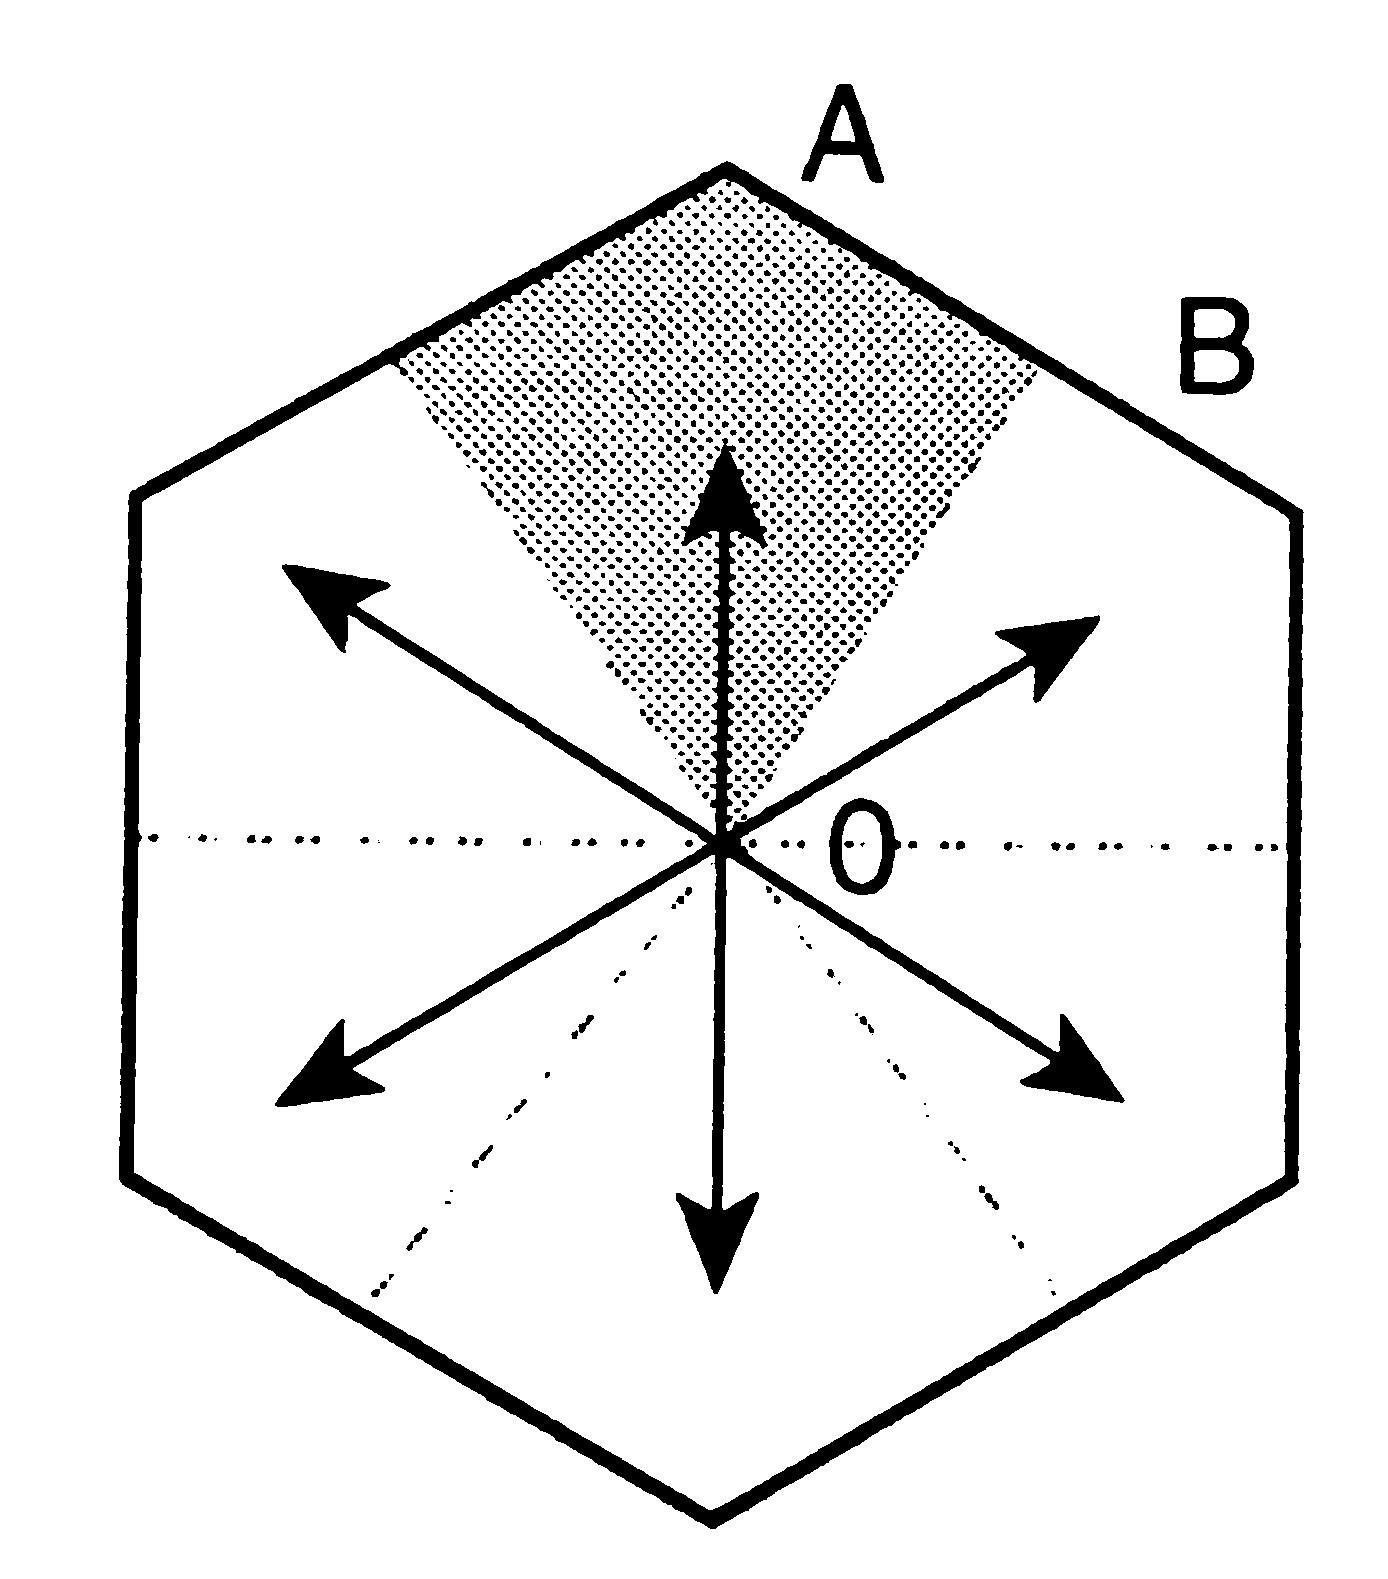
\includegraphics[scale=0.1]{imagenes/comunicaciones_moviles/cm_cap4_6_fixed.jpg}}
%\end{figure}

El diseño de celdas elegido determina directamente los efectos debidos a la propagación.
Se puede usar un diseño \textit{estático}, en el que la frecuencia asignada a cada sector o celda es siempre la misma. Este es el caso de los sistemas de segunda y tercera generación.
Otra posibilidad, más avanzada, es controlar dinámicamente los recursos (frecuencias) utilizados en cada célula en función de la interferencia intercelular existente.
Estas técnicas constituyen métodos \textit{dinámicos} de reutilización de frecuencias, y se suelen denominar ICIC (\textit{Inter-Cell Interference Coordination}) \cite{RefWorks:80}.

\subsection{Procesado de señal}

Como se ha descrito en el epígrafe \textit{Transmisión inalámbrica}, el canal físico de comunicaciones es el elemento que más atención merece en el sistema de comunicaciones móviles.
La señal que se transmite se debe diseñar tanto para implementar diversas funcionalidades del sistema de comunicaciones móviles como para paliar los efectos indeseados.

En suma, se recurre a numerosas técnicas de procesado de señal.

\paragraph{Acceso múltiple}

Permite a los terminales del sistema móvil compartir los recursos comunes de la red a través de las estaciones base \cite{RefWorks:77}.
En los sistemas celulares, el acceso múltiple comprende únicamente el enlace ascendente, pues los terminales compiten por comunicarse con la estación base.
Se denomina canal físico a la facilidad concedida a un usuario mediante la cual éste puede acceder al sistema
y las técnicas de multiacceso son procedimientos de asignación de canales físicos a las estaciones.
El acceso múltiple puede tener lugar separando a los usuarios en recursos de frecuencia (\textit{Frequency Division Multiple Access}, FDMA), tiempo (\textit{Time Division Multiple Access}, TDMA), espacio (\textit{Space Division Multiple Access}, SDMA) y código (\textit{Code Division Multiple Access}, CDMA) \cite{RefWorks:78}.

\paragraph{Multiplexación}

Permite a los terminales del sistema móvil compartir los recursos comunes de la red a través de las estaciones base \cite{RefWorks:77}.
En los sistemas celulares, la multiplexación comprende únicamente el enlace descendente, pues los terminales compiten por obtener un flujo de comunicaciones de la estación base.
La multiplexación aplica los mismos principios técnicos que el acceso múltiple y sus distintas soluciones son complementarias a las del mismo.
La multiplexación puede tener lugar separando a los usuarios en recursos de frecuencia (\textit{Frequency Division Multiplex}, FDM), tiempo (\textit{Time Division Multiplex}, TDM), espacio (\textit{Space Division Multiplex}, SDM) y código (\textit{Code Division Multiplex}, CDM) \cite{RefWorks:78}.

\paragraph{Duplexación}

Permite al sistema operar modo \textit{dúplex}, en el cual es posible la transmisión y recepción simultáneas en todas las estaciones \cite{RefWorks:77}.
La duplexación puede tener lugar separando a los usuarios en recursos de frecuencia (\textit{Frequency Division Duplexing}, FDD) y tiempo (\textit{Time Division Duplexing}, TDD) \cite{RefWorks:78}.

\paragraph{Diversidad}

La diversidad permite mejorar la calidad de recepción de la señal.
La mejora obtenida por esta técnica se basa en la posibilidad de tener dos o más versiones de la señal recibida,
afectadas de manera diferente por los fenómenos de propagación, y en particular por el desvanecimiento.
La diversidad puede ser de recepción, si el receptor es capaz de percibir dos señales separadas en recursos de transmisión (caso más común en el enlace ascendente),
o de transmisión, si el transmisor es capaz de generar dos señales separadas en recursos de transmisión (caso más común en el enlace descendente).
La diversidad puede tener lugar separando a las señales en recursos de frecuencia, tiempo, espacio y polarización \cite{RefWorks:78}.

\paragraph{Modulaciones}

La modulación es la forma que el transmisor da a la señal que se transmite.
Es una solución de alto nivel en el conjunto del sistema de comunicaciones al integrar diversas funcionalidades
(transmisión de información, acceso múltiple, multiplexación, paliar diversos problemas de la transmisión inalámbrica).
El diseño de una modulación comprende también las tareas de ecualización y detección, que se aplican en el receptor.
Los sistemas de segunda y tercera generación utilizan modulaciones digitales de portadora única (MSK, GMSK, $\pi / 4$-DPSK, M-QAM).
Los sistemas de cuarta y quinta generación utilizan la modulación digital con multiportadora (\textit{Orthogonal Frequency Division Multiplex}, OFDM),
que permite utilizar el esquema de QPSK o M-QAM al tiempo que se logra una mejor capacidad para resistir las perturbaciones que aparecen en el canal de propagación
\cite{RefWorks:84, RefWorks:85, RefWorks:86, RefWorks:87, RefWorks:78, RefWorks:80, RefWorks:26}

\paragraph{Codificación de canal}

Consiste en transmitir, en lugar de la secuencia de bits dada, otra derivada de la original mediante un algoritmo.
La secuencia original es recuperada en el receptor mediante un algoritmo complementario.
Es una solución de alto nivel en el conjunto del sistema de comunicaciones al integrar diversas funcionalidades
(transmisión de información, acceso múltiple, multiplexación, paliar diversos problemas de la transmisión inalámbrica).
%	En especial, se aprecian sus capacidades para detectar y corregir errores (\textit{Forward Error Correction}, FEC).
\cite{RefWorks:89, RefWorks:78}

\paragraph{Técnicas multiantena (\textit{Multiple Input Multiple Output}, MIMO)}

Los sistemas MIMO se basan en la existencia de múltiples antenas en el transmisor, en el receptor o ambos para mejorar ciertas características  de la transmisión.
%	El canal de propagación será en general diferente entre cada pareja de antenas transmisora y receptora.
%	No obstante, existe un cierto grado de \textit{correlación espacial}: las respuestas de los canales definidos entre antenas diferentes serán más parecidas entre sí cuanto más próximas estén ubicadas dichas antenas.
\cite{RefWorks:79}
El conjunto de antenas se denomina \textit{agrupación} o \textit{array}.
El uso de agrupaciones permite nuevas soluciones de procesado espacial, como la formación de un haz directivo (\textit{beamforming}) o la codificación espacial.
En general, el sistema MIMO puede funcionar en modo de \textit{incremento de la capacidad} / \textit{multiplexación espacial}, transmitiendo distintas señales en las distintas antenas,
o en modo de \textit{diversidad espacial} / \textit{ganancia de potencia}, transmitiendo la misma señal en distintas antenas, lo que crea redundancia de la señal.
\cite{RefWorks:80}
De esta manera, las técnicas MIMO contribuyen a las funcionalidades de la transmisión de información, de acceso múltiple, de multiplexación y resuelven algunos problemas de la transmisión inalámbrica.
\cite{RefWorks:78}

\paragraph{Espectro ensanchado (\textit{Spread Spectrum}, SS)}

El espectro ensanchado es una modalidad de transmisión donde la señal transmitida ocupa una anchura de banda $W$ mucho mayor que la anchura de banda $B$ de la señal de información.
Para realizar el ensanchamiento se utiliza una secuencia denominada código de ensanchamiento, secuencia código o signatura.
La señal SS se recupera, en recepción, aplicando el mismo código en un proceso de desensanchamiento.
%	Las técnicas de espectro ensanchado ofrecen ventajas en cuanto a inmunidad frente a interferencias y aprovechamiento del efecto del multitrayecto.
De esta manera, las técnicas SS contribuyen a las funcionalidades de acceso múltiple, de multiplexación y resuelven algunos problemas de la transmisión inalámbrica.
\cite{RefWorks:78, RefWorks:87}

\subsection{Otras técnicas avanzadas}

Los sistemas de tercera generación en adelante incorporan una serie de soluciones que se sustentan sobre los principios expuestos en los epígrafes anteriores.
Estas soluciones sobrepasan el límite de una sola capa de la pila de protocolos, abarcando varios niveles del sistema para su funcionamiento.

Estas soluciones permiten a las nuevas tecnologías alcanzar las metas de tasa binaria, probabilidad de error, latencia y eficiencia espectral impuestas.
Es por ello que de entre las técnicas descritas se destacan las de gestión de recursos radioeléctricos (\textit{Radio Resource Management}, RRM),
al permitir administrar de una manera más avanzada y eficiente la utilización de estos recursos.

\subsubsection{HARQ}

Las técnicas HARQ (\textit{Hybrid Automatic Retransmission Request}) son un caso de RRM.
En ellas, la señal se divide en bloques de bits, a cada bloque se le aplica un código corrector y un código detector.
Cada bloque recibido se decodifica primero con el código corrector.
Cuando éste no puede corregir todos los errores, el bloque se considera incorrecto.
Esta situación se detecta mediante el código detector, y si es necesario se solicita la retransmisión del bloque de bits.
\cite{RefWorks:26, RefWorks:80}

Existe una variante de esta técnica, \textit{HARQ con combinación de retransmisiones}.
Cuando se recibe un bloque incorrecto (es decir, con errores que no han podido corregirse), en vez de descartarse se almacena.
Después, cuando se recibe la versión retransmitida del bloque, ésta se combina con las (re)transmisiones anteriores del mismo bloque.
\cite{RefWorks:26, RefWorks:80}

\subsubsection{Planificación de paquetes o planificación de usuarios}

Las técnicas de planificación de paquetes (\textit{packet scheduling} ó \textit{scheduling}) son un caso de RRM.
La transmisión de información de tráfico se realiza mediante uno o varios canales compartidos por los usuarios de la célula o sector.
La planificación de paquetes es la funcionalidad de la red que controla a qué usuario se transmite (enlace descendente) o se le permite transmitir (enlace ascendente) dentro de esos canales compartidos.
Determina, por tanto, cómo distribuir los recursos de transmisión a los diferentes usuarios.
\cite{RefWorks:80}

En el caso de la modulación OFDM, los recursos son de tiempo y frecuencia.
Ambas variables se dividen en tramos, dando lugar a una \textit{rejilla de recursos} que se asignan a los usuarios según el criterio del planificador.
\cite{RefWorks:26, RefWorks:80}

%\subsubsection{Elementos de la arquitectura y las interfaces}
%
%Comprende el uso de canales desde 3G para implementar funcionalidades y ordenar procesos. En particular, el uso de canales físicos y señales permite implementar RRM y ordenan el proceso de RRM.
%\cite{RefWorks:26, RefWorks:81}

\subsubsection{Adaptación de enlace}

Las técnicas de adaptación de enlace son un caso de RRM.
Se entiende por adaptación al canal radio cualquier procedimiento que modifique los parámetros de la transmisión en función del estado del canal.
Los parámetros de la transmisión que se pueden modificar son, entre otros, la potencia, modulación o tasa de codificación de canal.
Los objetivos pueden ser, por ejemplo, maximizar la tasa binaria neta (\textit{throughput}) o conseguir una tasa binaria fija con un retardo acotado.
\cite{RefWorks:80}

El enfoque seguido en los modernos sistemas de comunicaciones móviles es variar la tasa binaria (\textit{Adaptative Modulation and Coding}, AMC).
Para ello, se modifican la modulación y la tasa de codificación de canal (\textit{Modulation and Coding Scheme}, MCS).
Para ello, el transmisor tiene información sobre el estado del canal.
La información es proporcionada por los \textit{informes de calidad del canal} (\textit{Channel Quality Indicator}, CQI), que se generan en la capa física.
Se puede conocer el canal de cada usuario, esto es, sus recursos de transmisión.
\cite{RefWorks:26, RefWorks:80}

\subsubsection{Categoría de terminal}

Ya en los sistemas de comunicaciones móviles de tercera generación se definen diferentes categorías de terminales en función de qué características incluyen,
tales como modulaciones o número máximo de canales de un tipo.
\cite{RefWorks:92}
En los sistemas de comunicaciones móviles de cuarta generación se han establecido diferentes clases de terminales UE según
sus capacidades de transmisión/recepción de datos,
tamaño del \textit{buffer} de recepción para HARQ
y número de capas de multiplexación espacial.
\cite{RefWorks:81}

El establecimiento de distintas categorías de terminales se puede considerar un caso de RRM.

\subsubsection{Novedades de \textit{LTE-Advanced}}

La especificación \textit{Release 10} (\textit{LTE-Advanced}) incluye todas las características de la especificación \textit{Release 8/9} (LTE) y añade algunas nuevas,
las más importantes se explican a continuación.
Estas características nuevas permiten que los sistemas de comunicaciones móviles de cuarta generación logren las metas impuestas por \textit{IMT-Advanced} y añaden nuevas dinámicas de la red de comunicaciones móviles que debemos atender.
\cite{RefWorks:39}

\paragraph{Agregación de portadoras}

La agregación de portadoras (\textit{Carrier Aggregation}, CA) responde a un enfoque del problema de transmisión:
el modo más inmediato de aumentar la capacidad es incrementar la anchura de banda. Ahora bien, por motivos de regulación no parece posible, al menos, a corto plazo, disponer de frecuencias portadoras de anchura de banda superiores a los 20 MHz previstos para LTE.
\cite{RefWorks:81, RefWorks:26}

Las mayores anchuras solo pueden conseguirse agregando portadoras, esto es, seleccionando varias portadoras independientes de ancho $b_i$ para servir como una única portadora de ancho:
$$B = \sum_i b_i$$
Cada una de las portadoras que se juntan se llama portadora componente (\textit{component carrier}) o solamente componente.
\cite{RefWorks:81, RefWorks:39}

\paragraph{MIMO avanzado}

LTE soportaba una gran cantidad de técnicas multiantena desde ya la especificación \textit{Release 8}.
Esta incluía diversidad en transmisión en el enlace descendente mediante SFBC (\textit{space-frequency block coding})
y SFBC combinado con FSTD (\textit{frequency shift time diversity}),
ambos para el caso de dos antenas en el transmisor.
También se soportaban técnicas en el enlace descendente que permitían la transmisión multicapa (multiplexación espacial) con hasta cuatro capas,
incluyendo la posibilidad de adaptación para transmitir con una sola capa, lo que resultaba en un caso de formación de haz (\textit{codebook-based beamforming}),
además de una forma básica de MIMO multiusuario (\textit{multi-user MIMO}) donde diferentes capas del mismo recurso de tiempo-frecuencia se pueden asignar a distintos terminales.
\cite{RefWorks:39, RefWorks:26}

En la especificación \textit{Release 10}, la multiplexación espacial en el enlace descendente se expande para soportar hasta ocho capas en el transmisor.
También se da soporte a la multiplexación espacial en el enlace ascendente con hasta cuatro capas.
\cite{RefWorks:39}

\paragraph{Redes heterogéneas}

La tasa binaria lograda por el usuario en un despliegue práctico depende de diversos factores:
la distancia entre el terminal y la estación base, si el usuario está en el interior o en el exterior, etc.
Una manera de incrementar la tasa binaria y la capacidad conjunta es hacer más densa la red celular, incrementando la cantidad de estaciones base por unidad de superficie.
En ciertos escenarios, como cuando los usuarios se agrupan en un lugar del espacio, existe otra posibilidad más interesante como complementar una macrocelda (\textit{macro cell}, estación base de gran capacidad y área de cobertura) con varias picoceldas (\textit{pico cell}, estación base de baja potencia) allá donde acudan los usuarios.
El resultado se denomina red heterogénea (\textit{Heterogeneous Network}, HetNet).
\cite{RefWorks:39, RefWorks:26}

Las redes heterogéneas ya eran posibles en las especificaciones de LTE (\textit{Release 8} y \textit{Release 9}), pero en la especificación de \textit{LTE-Advanced} (\textit{Release 10}) se ñaden nuevas características.
\cite{RefWorks:39}

\paragraph{Nodos repetidores}

Los nodos repetidores (\textit{Relay Nodes}, RN) son estaciones base de baja potencia que se conectan a un eNB convencional llamado nodo donante DeNB (\textit{Donor eNB}), reciben la señal de este nodo, realizan su procesamiento con regeneración digital y la retransmiten a su zona de cobertura.
En sentido ascendente los repetidores captan la señal de los móviles y la retransmiten a la base.
\cite{RefWorks:81, RefWorks:39}

\paragraph{Transmisión multipunto coordinada}

El objetivo de la transmisión multipunto coordinada (\textit{Coordinated Multi Point}, CoMP) es el aumento del caudal o tasa binaria en el borde de la célula y, en consecuencia, el incremento del caudal medio en la célula.
Para ello se habilitan posibilidades de conexión de un UE situado en el borde con dos o más eNB, transmisores en DL o receptores en UL que pueden estar en la misma ubicación y diferentes sectores (CoMP intracelular) o en diferentes emplazamientos (CoMP intercelular).
\cite{RefWorks:81, RefWorks:39, RefWorks:26}

\subsubsection{Novedades de 5G}

Las especificaciones de 3GPP para la quinta generación de comunicaciones móviles introducen una serie de tecnologías que se presuponen disruptivas:
seccionamiento de la red (\textit{Network Slicing}), virtualización de funciones de red (\textit{Network Function Virtualization}, NFV), computación en el borde de la red (\textit{Multi-access Edge Computing}, MEC).
Pese a ello, algunas de estas tecnologías, como el seccionamiento de la red o la característica MEC, no tienen repercusión en el funcionamiento de la interfaz de radio al estar sus funcionalidades delimitadas de manera estricta a la red de tránsito.
Por otro lado, la característica NFV, pese a modificar algunos de los planteamientos con los que se constituye la red de acceso, éstos siguen siendo análogos a los que se usaban en las anteriores generaciones de comunicaciones móviles, manteniéndose las mismas funcionalidades básicas de la interfaz de radio.
\cite{RefWorks:47}

Es por esto, que no tendremos en cuenta estas novedades de 5G para describir la interfaz de radio.

\section{Interfaz de radio de 5G}

La interfaz de radio del sistema de comunicaciones móviles de quinta generación (\textit{Fifth Generation of Mobile Telephony}, \textit{5G System}, 5G ó 5GS) se denomina NR (\textit{New Radio}).
NR toma los fundamentos expuestos en el epígrafe \textit{Fundamentos de comunicaciones móviles},
todos ellos concebidos para los sistemas de comunicaciones móviles de segunda, tercera y cuarta generación.
Las tecnologías desarrolladas hasta la especificación \textit{Release 10} (\textit{LTE-Advanced}) se perfeccionan y se expanden sus posibilidades para mejorar las prestaciones de 5G.

Se añaden, además, nuevos servicios, conformando el conjunto de servicios que se ofrecerán en 5G: \textit{Enhanced Mobile Broadband} (eMBB), \textit{Critical Communications} (CC), \textit{Ultra Reliable and Low Latency Communications} (URLLC), \textit{Massive Internet of Things} (mIoT) y \textit{Flexible network operations}.
\cite{RefWorks:47}

5G queda establecido a partir de la especificación \textit{Release 15}.
\cite{RefWorks:47}

\subsection{Arquitectura de la red}

El sistema 5G se compone de los mismos elementos que las anteriores generaciones de comunicaciones móviles \cite{RefWorks:47}:
\begin{itemize}
\item Terminal de usuario (\textit{User Equipment}, UE).
\item Red de acceso por radio de nueva generación (\textit{New Generation Radio Access Network}, NG-RAN).
La entidad principal de la NG-RAN se denomina gNB (\textit{5G Node B}). Se trata, a grandes rasgos, de la estación base.
La gNB se puede dividir en una \textit{unidad central} (\textit{gNB-Central Unit}, gNB-CU) y una o más \textit{unidades distribuidas} (\textit{gNB-Distributed Unit}, gNB-DU).
\item Núcleo de red (\textit{5G Core Network}, 5GC).
En relación a la interfaz de radio, se destacan las entidades UPF (\textit{User Plane Function}), que maneja los datos del usuario, y AMF \textit{Access and Mobility management Function}), que se encuentra en el plano de señalización y accede al UE y a la NG-RAN.
\end{itemize}

\begin{figure}[H]
	\ffigbox[\FBwidth] {
	\caption[Interfaz de radio de 5G]{Interfaz de radio de 5G: Panorámica del sistema 5G.
	Aquí, la 5GC se representa esquemáticamente con la entidad AMF/UPF.

	Fuente: \cite{RefWorks:47}}
	}
	{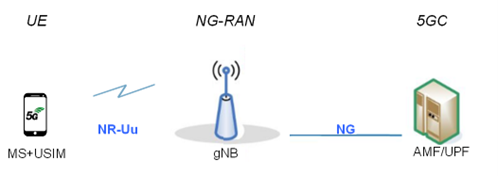
\includegraphics[scale=1.0]{imagenes/3gpp_5g_system_overview/5g-fig1.png}}
\end{figure}

La arquitectura del sistema 5G se considera una arquitectura basada en servicios (\textit{Service-Based Architecture}, SBA),
donde los elementos que la componen se definen en términos de funciones de red (Network Functions, NF) en lugar de las entidades de red tradicionales.
A través de las interfaces que también se definen en las especificaciones, cualquier NF puede ofrecer sus servicios a otras NF autorizadas o a cualquier consumidor autorizado para acceder a esos servicios.
Este planteamiento ofrece modularidad y reusabilidad a los equipos desarrollados para el sistema de 5G.
\cite{RefWorks:47}

Si nos ceñimos a las interfaces relacionadas con la interfaz de radio, es decir, omitiendo las que pertenecen estrictamente a la red de tránsito, podemos nombrar:
\begin{itemize}
\item La interfaz de radio se denomina NR-Uu (\textit{New Radio Uu}), enlaza el UE con la gNB.
\item La interfaz F1 enlaza las entidades gNB-CU y gNB-DU.
\item El punto de referencia entre la NG-RAN y la 5GC se denomina \textit{NG}.
Éste, en realidad, está constituido por varias interfaces, como N2 ó N3.
\end{itemize}

\begin{figure}[H]
	\ffigbox[\FBwidth] {
	\caption[Elementos de 5G]{Principales NF de 5G:
	En la figura, el plano de usuario, es decir, las NF y elementos involucrados en el transporte de datos de usuario, se muestra en el nivel bajo,
	mientras que en los niveles superiores se muestran las NF esenciales en el plano de señalización.
	Se pueden ver las interfaces que conectan las distintas NF.

	Fuente: \cite{RefWorks:47}}
	}
	{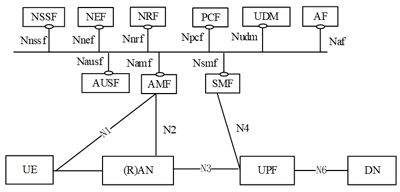
\includegraphics[scale=1.0]{imagenes/3gpp_5g_system_overview/5g-fig2.png}}
\end{figure}

En la interfaz de radio también se usan canales físicos y señales físicas como las de LTE para implementar los protocolos de la capa física.
\cite{RefWorks:44}

En cuanto a los protocolos, se define una pila para la comunicación entre las NF.
\cite{RefWorks:47}.
%No es necesario describirlos para la interfaz de radio.
%Destacan:
%\begin{itemize}
%\item En el plano de control: NAS-SM, NAS-MM, capa de protocolos 5G-AN, NG-AP, SCTP.
%\item En el plano de usuario: capa PDU, GTP U, capa de protocolos 5G-AN, UDP/IP.
%\end{itemize}
En relación a la interfaz de radio, esto es, concernientes a las entidades UE y gNB, destacamos varios niveles de la pila de protocolos \cite{RefWorks:7}:
\begin{enumerate}
\item La capa física o \textit{capa PHY} (\textit{PHY layer}):
Comprende los procedimientos para transmitir y recibir señal por el canal de radio.
También se llevan a cabo tareas que permiten generar los informes CQI.
\item La capa de enlace o \textit{capa MAC} (\textit{MAC layer}):
En ella tienen lugar los procesos que asignan los recursos de radio (RRM) para servir al tráfico demandado.
%principalmente descritos en las especificaciones 3GPP 38.214 y 3GPP 38.211.
%Esto incluye la planificación de paquetes o la implementación del modo dúplex mediante TDD ó FDD,
%ambos aprovechando la flexibilidad que ofrece OFDM para dividir los recursos tiempo-frecuencia.
\item La capa de red o \textit{capa PDCP/RLC} (\textit{PDCP/RLC layer}):
Maneja los paquetes IP que deben se transmiten o reciben de acuerdo con los procedimientos de la capa MAC,
que es la que modera el flujo de información a través de la interfaz de radio.
\end{enumerate}

Adicionalmente, se han definido dos modos de despliegue del sistema de 5G \cite{RefWorks:47}:
\begin{itemize}
\item Arquitectura de \textit{5G no por separado} (\textit{Non-Stand Alone}, NSA):
Se usan NG-RAN y NR en conjunto con infraestructura de LTE, en particular con su red de acceso (E-UTRAN) y su núcleo de red (EPC).
Esto permite el despliegue paulatino de 5G sin tener que reemplazar toda la infraestructura de redes existente.
En esta modalidad, solo se da soporte a los servicios de 4G, pero ya se pueden apreciar las capacidades de NR.
\begin{figure}[H]
	\ffigbox[\FBwidth] {
	\caption[5G NSA]{Arquitectura de 5G NSA:
	Se pueden ver las estaciones base de 4G (eNB) y 5G (en-gNB) conformando la red de acceso de 4G (E-UTRAN).
	Ésta se conecta al núcleo de red de 4G (EPC).
	Se usan las interfaces definidas para 4G.

	Fuente: \cite{RefWorks:47}}
	}
	{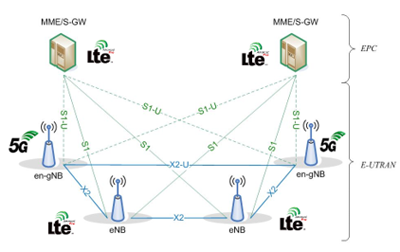
\includegraphics[scale=1.0]{imagenes/3gpp_5g_system_overview/5g-fig5.png}}
\end{figure}
\item Arquitectura de \textit{5G por separado} (\textit{Stand-Alone}, SA):
Se usan NG-RAN y NR en conjunto con el núcleo de red de 5G.
Se da soporte a todos los servicios de 5G y se aprecian todas sus capacidades.
\begin{figure}[H]
	\ffigbox[\FBwidth] {
	\caption[5G SA]{Arquitectura de 5G SA:
	Se pueden ver las estaciones base de 5G (gNB) conformando la red de acceso de 5G (NG-RAN).
	Ésta se conecta al núcleo de red de 5G (5GC).
	Se usan las interfaces definidas para 5G.

	Fuente: \cite{RefWorks:47}}
	}
	{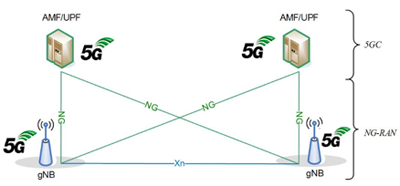
\includegraphics[scale=1.0]{imagenes/3gpp_5g_system_overview/5g-fig6.png}}
\end{figure}
\end{itemize}

\subsection{Transmisión inalámbrica}

La señal transmitida por la interfaz radio de 5G es sujeto de alteraciones como las estudiadas en el epígrafe \textit{Transmisión inalámbrica}.
\cite{RefWorks:7}
Las especificaciones de 5G incluyen avanzados modelos de canal para poder simular fenómenos como la atenuación, el desvanecimiento lento y el desvanecimiento rápido.
\cite{RefWorks:46}

\subsection{Sistema celular}

Usa un sistema celular moderno, con estaciones repartidas para dar cobertura.
Al igual que \textit{LTE-Advanced}, permite el uso de celdas de distintas clases (HetNet), nodos repetidores (RN) y coordinación de celdas (CoMP).
\cite{RefWorks:47}

En cuanto a la asignación de frecuencias, se usan múltiples rangos de frecuencias para permitir el despliegue en frecuencias siguiendo el criterio de cada país o región.
Las portadoras van de 400 MHz a 100 GHz, pero las bandas licenciadas van de 600 MHz a 39 GHz.
En muchos casos se trata de bandas recicladas de TV (UHF) y sistemas satelitales,
lo que no da lugar a interferencias ya que la asignación y atribución cuidan de que no haya coincidencias en la misma ubicación.

Para las redes móviles terrestres, se usan tres rangos de frecuencias:
\begin{itemize}
\item Hasta 1 GHz: Mejor propagación.
Este conjunto se pretende usar para cubrir grandes áreas (despliegues rurales).
Las portadoras pueden tener un ancho de hasta 100 MHz.
\item De 1 GHz a 6 GHz: Este conjunto se pretende usar despliegues urbanos y suburbanos.
Las portadoras pueden tener un ancho de hasta 100 MHz.
\item A partir de 6 GHz: Peor propagación.
Este conjunto se pretende usar para cubrir los entornos urbanos más densos (\textit{hot-spot}).
Las portadoras pueden tener un ancho de hasta 400 MHz.
\end{itemize}

En el caso de España, contemplamos varias acciones independientes orientadas a conformar el escenario de despliegue de 5G en lo que a frecuencias y cobertura se refiere \cite{RefWorks:72}:

\begin{itemize}
\item En junio de 2019 se aprobó el nuevo \textit{Plan Nacional Técnico de la TDT}, que regula los principales aspectos de la liberación de la banda de 700 MHz.
\item {
Se ha habilitado y licenciado una parte del espectro radioeléctrico para las tecnologías de 5G:
\begin{itemize}
\item La banda de 3,6-3,8 GHz fue licitada en julio de 2018.
\item La banda de 700 MHz fue licitada en 2020.
\end{itemize}
}
\item Se ha apoyado la realización de experiencias a través de proyectos experimentales con la concesión
de apoyos económicos directos.
\end{itemize}

\subsection{Procesado de señal}

La interfaz radio de 5G tiene un complejo sistema que bebe de las experiencias de las anteriores generaciones de telefonía móvil.
Con la excepción del espectro ensanchado, se puede decir que se usan todas las soluciones expuestas en el epígrafe \textit{Procesado de señal}.
\cite{RefWorks:7}


\paragraph{Modulaciones}

Como se indicó en el epígrafe \textit{Fundamentos de comunicaciones móviles}, los sistemas de quinta generación usan la modulación OFDM para hacer frente a las adversidades de la transmisión inalámbrica.
En el enlace descendente (DL), NR usa OFDM con prefijo cíclico (\textit{Cyclic Prefix}, CP).
En el enlace ascendente (UL), NR puede usar OFDM o una variante denominada \textit{OFDM con precodificación de transformada discreta de Fourier} (DFT-s-OFDM),
que mejora la cobertura porque reduce la relación de pico a promedio de potencia (\textit{peak-to-average power ratio}, PAPR) y está limitado a la transmisión con una sola capa.
\cite{RefWorks:47}

OFDM permite dividir los recursos de tiempo-frecuencia en una malla,
a partir de la que se realiza su asignación mediante los procedimientos de la capa MAC \cite{RefWorks:7, RefWorks:44, RefWorks:42}.
\begin{enumerate}
\item {
La malla se divide en:
\begin{itemize}
\item Frecuencia:
El gNB tiene un ancho de banda fijo asignado para transmisión/recepción.
El ancho de banda total se divide en subportadoras de tamaño fijo (su tamaño varía en función de la numerología usada).
Los tramos de frecuencia en que se puede dividir el ancho de banda son jerárquicos:
pueden ser del ancho de banda al completo (trama), de 12 portadoras consecutivas (\textit{Resource Block}, RB) y de una sola subportadora.
\item Tiempo:
El tiempo se divide en tramos temporales.
Las unidades que se pueden asignar y también permiten sincronizar los procesos de la interfaz de radio y delimitar su duración.
Los tramos en que se divide el tiempo son jerárquicos:
pueden ser de 10 ms (trama), de 1 ms (subtrama) y de duración inferior a 1 ms (\textit{slot}, su duración varía en función de la numerología usada).
\end{itemize}

\begin{figure}[H]
	\ffigbox[\FBwidth] {
	\caption[Recursos OFDM]{Malla de recursos tiempo-frecuencia en OFDM:
	Se pueden asignar recursos correspondientes a un instante o a una portadora a un UE.

	Fuente: \cite{RefWorks:7}}
	}
	{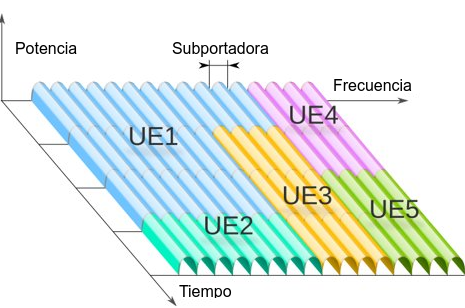
\includegraphics[scale=1.0]{imagenes/fikore_doc/figures/Grid_es.png}}
\end{figure}
}
\item {
Esta división en tiempo y frecuencia ofrece una gran flexibilidad y granularidad para asignar los recursos de radio.
Las unidades de menor tamaño (1 \textit{slot} $\times$ 1 subportadora) se denominan \textit{Resource Element} (RE).
Los RE se agrupan en \textit{Physical Resource Blocks} (PRB) y éstos, a su vez, en \textit{Resource Block Groups} (RBG) para su asignación.
Sólo se asignan los PRB y los RBG.
\item {
Como se ha indicado, existe una configuración, la numerología, que determina las dimensiones de las unidades de tiempo-frecuencia:

\begin{figure}[H]
	\ffigbox[\FBwidth] {
	\caption[Numerología]{Numerología en 5G.

	Fuente: \cite{RefWorks:7}}
	}
	{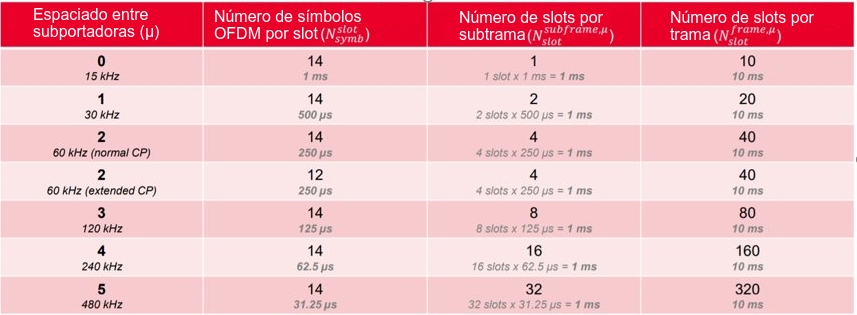
\includegraphics[scale=0.65]{imagenes/fikore_doc/figures/Numerology_es.png}}
\end{figure}
}
\item {
Se puede seleccionar entre distintas modulaciones: QPSK (2 bits), 16-QAM (4 bits), 64-QAM (6 bits), 256-QAM (8 bits).
La selección de la modulación la lleva a cabo el proceso de AMC, que asigna una modulación distinta a un PRB ó a un RBG.
}
\item Se estima un tamaño de bloque (\textit{Transport Block Size}, TBS) en bits que es el que puede manejar la interfaz de radio.
Este TBS se da a conocer a la capa PDCP/RLC, que se encarga de manejar los paquetes IP.
\item Se usa la misma rejilla de recursos de tiempo-frecuencia para implementar la transmisión dúplex.
Tanto FDD como TDD se pueden implementar al dividir sus respectivos dominios en tramos dedicados a la transmisión en el enlace ascendente o en el enlace descendente.
\item {
La implementación de estas funcionalidades se lleva a cabo mediante los canales físicos y señales físicas.
Un canal físico es una sección de los recursos de tiempo-frecuencia que se reserva para las funcionalidades de la capa física.

\begin{figure}[H]
	\ffigbox[\FBwidth] {
	\caption[Canales físicos]{Ejemplo de canales físicos:
	Estructura en tiempo-frecuencia de la trama del enlace descendente en LTE para el caso de un ancho de banda de 3 MHz (ejemplo con tres símbolos OFDM dedicados a canales de control).

	En 5G se usa un procedimiento muy similar, heredado de LTE.

	Fuente: \cite{RefWorks:26}}
	}
	{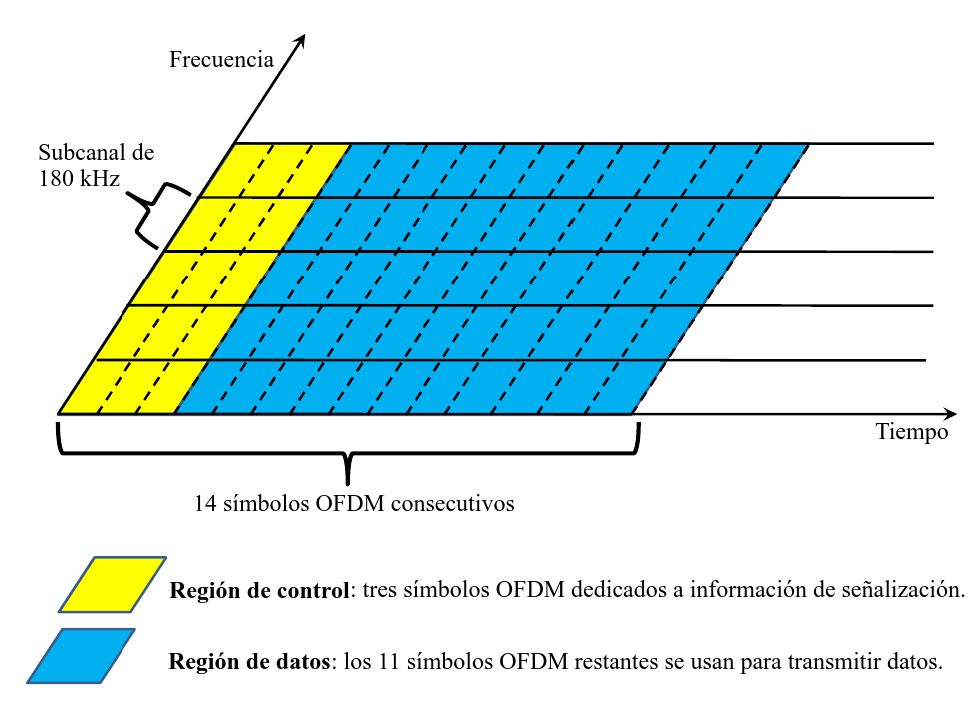
\includegraphics[scale=0.5]{imagenes/scheduling_italianos/scheduling_italianos-173_es.png}}
\end{figure}
}
\end{enumerate}

\paragraph{MIMO}

5G incorpora mejoras de las técnicas multiantena ya existentes en \textit{LTE-Advanced}
\cite{RefWorks:42}
y una nueva modalidad denominada MIMO \textit{Over-the-Air} (OTA).
\cite{RefWorks:71}

\subsection{Otras técnicas avanzadas}

En 5G se usan todas las técnicas expuestas en el epígrafe \textit{Otras técnicas avanzadas}.
Por su importancia en la interfaz de radio, destacan.
\begin{itemize}
\item HARQ:
La capa MAC se ocupa de retransmitir los bloques que no han podido ser recuperados, siguiendo un esquema HARQ.
\cite{RefWorks:7}
\item Planificación de paquetes:
A partir del conocimiento del canal gracias al CQI, siguiendo un criterio establecido (métricas), se pueden asignar distintos PRB/RBG a uno u otro usuario.
\cite{RefWorks:7}
\item Adaptación de enlace:
A partir del conocimiento del canal gracias al CQI,
la capa MAC modifica el esquema de modulación (MCS) usado para la transmisión/recepción por cada UE,
que puede ser QPSK, 16-QAM, 64-QAM ó 256-QAM.
Se trata, por tanto, de un proceso de AMC.
\cite{RefWorks:7, RefWorks:42}
\item Agregación de portadoras:
5G incorpora mejoras de las técnicas multiportadora ya existentes en \textit{LTE-Advanced}.
\cite{RefWorks:44, RefWorks:42}
\end{itemize}

\section{Emulación del acceso radio 5G}

%\subsection{Simulación de sistemas de comunicaciones}

La interfaz de radio comprende varios aspectos que podemos tratar por separado para su simulación \cite{RefWorks:95}:
\begin{itemize}
\item Arquitectura (descripción funcional, protocolos e interfaces):
Estos elementos, en la práctica, se implementan mediante sistemas informáticos,
por lo que se pueden emular con cualquier sistema informático que iguale en capacidad al que se usa para la implementación.
Consideramos, además, los distintos escenarios de emulación que se pueden dar: tráfico real o tráfico simulado.
\item Transmisión inalámbrica:
La transmisión de señales moduladas, así como su alteración, se puede estudiar mediante las expresiones de la teoría de la comunicación.
El ruido y la interferencia son señales que se estudian mediante la estadística
y su efecto se puede computar usando modelos de canal y balances de enlace.
Por otro lado, la teoría de simulación de sistemas de comunicaciones considera el modelo de los sistemas para representar el canal de transmisión:
\begin{itemize}
\item Los sistemas lineales variantes en el tiempo son los adecuados para representar fenómenos complejos como el desvanecimiento rápido.
\item Los sistemas lineales invariantes en el tiempo son capaces de representar el desvanecimiento lento y la atenuación.
\item Los sistemas no lineales se reservan para estudiar el efecto de los amplificadores, especialmente cuando confluye el uso de amplificadores con el de modulaciones de PAPR elevada como OFDM.
\end{itemize}
\item Para aproximar los parámetros del sistema, como las probabilidad de error (BER), se utilizan soluciones clásicas: Monte Carlo, muestreo enfatizado, etc.
\end{itemize}

%\subsection{Emuladores y simuladores del sistema 5G}

Para este caso, existen los simuladores de RAN,
que permiten estudiar las prestaciones de un despliegue de la red de 5G, el cual, podrá usarse en una aplicación de 5G.
Entre los ejemplos más destacados están: \textit{Vienna Simulator}, \textit{NS-3}, \textit{Matlab 5G Toolbox}, \textit{5G-LENA}.
\cite{RefWorks:3, RefWorks:5}

También existen los emuladores de RAN de nivel de sistema,
que sustituyen la pila de protocolos al completo y son capaces de manejar tráfico real.
Esto permite estudiar directamente el rendimiento de una aplicación de 5G en un despliegue simulado.
Entre los ejemplos más destacados están: extensión de \textit{NS-3}, \textit{OpenAirInterface 5G-RAN}, \textit{Simu5G}, \textit{Polaris}, \textit{Keysight} y, finalmente, \textit{FikoRE}.
\cite{RefWorks:3, RefWorks:5}

\chapter{Emulador \textit{FikoRE}}

El programa informático \textit{Framework for Immersive communication networK Optimization RAN Emulator} (\textit{FikoRE}) es un emulador de nivel de sistema de la interfaz de radio de 5G.
Como tal, debe representar (simular) el comportamiento de la capa física (PHY) y de los protocolos que permiten su funcionamiento (MAC).
También debe ser compatible con una aplicación real, debe permitir la interacción de esta aplicación (emular) con un sistema que se comporte como la RAN de 5G;
el sistema debe ser capaz de cursar tráfico real (PDCP/RCL). \cite{RefWorks:5, RefWorks:3, RefWorks:7}

El emulador recrea las partes de 5G que conforman la interfaz de radio (PHY, MAC, PDCP/RLC), todas adscritas a la red de acceso (RAN).
Es necesario conocer las precisiones del emulador en función de los casos de uso que queremos estudiar.

\section{Características generales}

\subsection{Implementación}

En lo que respecta a la implementación, el emulador está programado en \textit{C++} y se puede ejecutar en una máquina \textit{Linux}. \cite{RefWorks:5, RefWorks:3, RefWorks:7}
Es modular, se compone de varias clases que podemos separar en los siguientes grupos \cite{RefWorks:5, RefWorks:3, RefWorks:7, RefWorks:100}:

%\begin{itemize}
%\item {
%	Terminal de usuario (UE):
%	\begin{itemize}
%	\item {
%		Simulación de PHY:
%		\begin{itemize}
%		\item \textit{src/phy\_layer}
%		\item \textit{src/phy\_shared}
%		\end{itemize}
%	}
%	\item {
%		Emulación de PDCP/RLC:
%		\begin{itemize}
%		\item \textit{src/pdcp\_layer}
%		\end{itemize}
%	}
%	\item {
%		Movilidad del UE:
%		\begin{itemize}
%		\item \textit{src/map}
%		\item \textit{src/mobility\_models}
%		\end{itemize}
%	}
%	\item {
%		Captura de tráfico IP:
%		\begin{itemize}
%		\item \textit{src/netfilter}
%		\end{itemize}
%	}
%	\item {
%		Otros comportamientos del UE (generación de tráfico IP, etc.):
%		\begin{itemize}
%		\item \textit{src/ue}
%		\end{itemize}
%	}
%	\end{itemize}
%}
%\item {
%	Estación base (gNB):
%	\begin{itemize}
%	\item {
%		Simulación de MAC:
%		\begin{itemize}
%		\item \textit{src/mac\_layer}
%		\end{itemize}
%	}
%	\end{itemize}
%}
%\end{itemize}

\begin{itemize}
\item {
	Terminal de usuario (UE):
	se ocupa de la simulación de PHY (módulos \textit{src/phy\_layer}, \textit{src/phy\_shared}),
	la emulación de PDCP/RLC (módulo \textit{src/pdcp\_layer}),
	la simulación de la movilidad del UE (módulos \textit{src/map}, \textit{src/mobility\_models}),
	la captura de tráfico IP (módulo \textit{src/netfilter})
	y la simulación de otros comportamientos del UE (generación de tráfico IP, etc.) (módulo \textit{src/ue}).
}
\item {
	Estación base (gNB):
	se ocupa de la simulación de MAC (módulo \textit{src/mac\_layer}).
}
\end{itemize}

\subsection{Flujo de información}

En lo que respecta al  flujo de información que permite la implementación de la interfaz de radio de 5G, en primer lugar consideramos los mismos componentes descritos en el anterior epígrafe.
Éstos reunen una serie de funcionalidades por separado \cite{RefWorks:5, RefWorks:3, RefWorks:7}:

\begin{itemize}
\item {
	Terminal de usuario (UE):
	Modela un UE particular. Estas funciones incluyen:
	\begin{itemize}
	\item Movilidad:
	Llevar a cabo la estimación de su posición mediante un modelo de movilidad elegido por el usuario.
	\item {
		Manejo de paquetes:
		\begin{itemize}
		\item Generar tráfico virtual mediante un modelo elegido por el usuario.
		\item Generar tráfico virtual tomando trazas de tráfico IP.
		\item Capturar tráfico real de unos puertos de la máquina seleccionados.
		\end{itemize}
	}
	\item Emulación de PDCP/RLC:
	Modelar el comportamiento de las capas RLC y PDCP con un gran nivel de abstracción.
	\item Simulación de PHY:
	Modelar las principales medidas de calidad del canal, como la SINR, la RSRP, las probabilidades de HARQ, etc.
	Implementa los modelos de la especificación 3GPP 38.901.
	\end{itemize}
}
\item Estación base (gNB):
Su cometido es la simulación de la capa MAC, incluyendo la asignación de recursos de radio.
Se siguen las indicaciones de las especificaciones 3GPP 38.214, 3GPP 38.211 y 3GPP 38.306.
\end{itemize}

Para implementa la funcionalidad de la interfaz de radio de 5G, estos componentes funcionan conjuntamente \cite{RefWorks:5, RefWorks:3}:

\begin{enumerate}
\item El tráfico de cada UE se genera o se captura mediante su módulo de generación/captura.
Los paquetes se envían a la capa RLC/PDCP, donde se encolan en el búfer IP.
\item Mediante una notificación especial (\textit{Scheduling Request}, SR), la capa PDCP/RLC notifica a la capa MAC cuántos bits hay disponibles para transmitir desde cada UE.
\item En paralelo, el módulo de la capa PHY estima los parámetros de calidad del canal (\textit{Channel State Information}, CSI) para cada UE.
\item Con la información de la SR y del CSI, la capa MAC asigna recursos tiempo-frecuencia a cada UE.
\item La capa PDCP/RLC layer, en concordancia con los recursos asignados por la capa MAC, segmenta los paquetes IP en bloques más pequeños.
Estos bloques son aquellos cuya transmisión por la interfaz de radio se debe simular.
\item Usando los parámetros de CSI, el módulo de la capa PHY determina la latencia de transmisión y las probabilidades de retransmisión con HARQ para cada bloque.
\item Si el bloque debe ser retransmitido, se coloca en la cola de HARQ correspondiente para ser asignado de nuevo.
\item Finalmente, si el bloque se transmite de manera exitosa, retorna al módulo de la capa RLC/PDCP.
Aquí, se comprueba la integridad y el orden de los paquetes IP completos.
\item Los paquetes IP que se han transmitido de manera exitosa se liberan de la cola.
Los corruptos o los perdidos se descartan.
\end{enumerate}

\begin{figure}[H]
	\ffigbox[\FBwidth] {
	\caption[Flujo de información de \textit{FikoRE}]{Flujo de información esquemático entre los principales módulos de \textit{FikoRE}.

	Fuente: \cite{RefWorks:3}}
	}
	{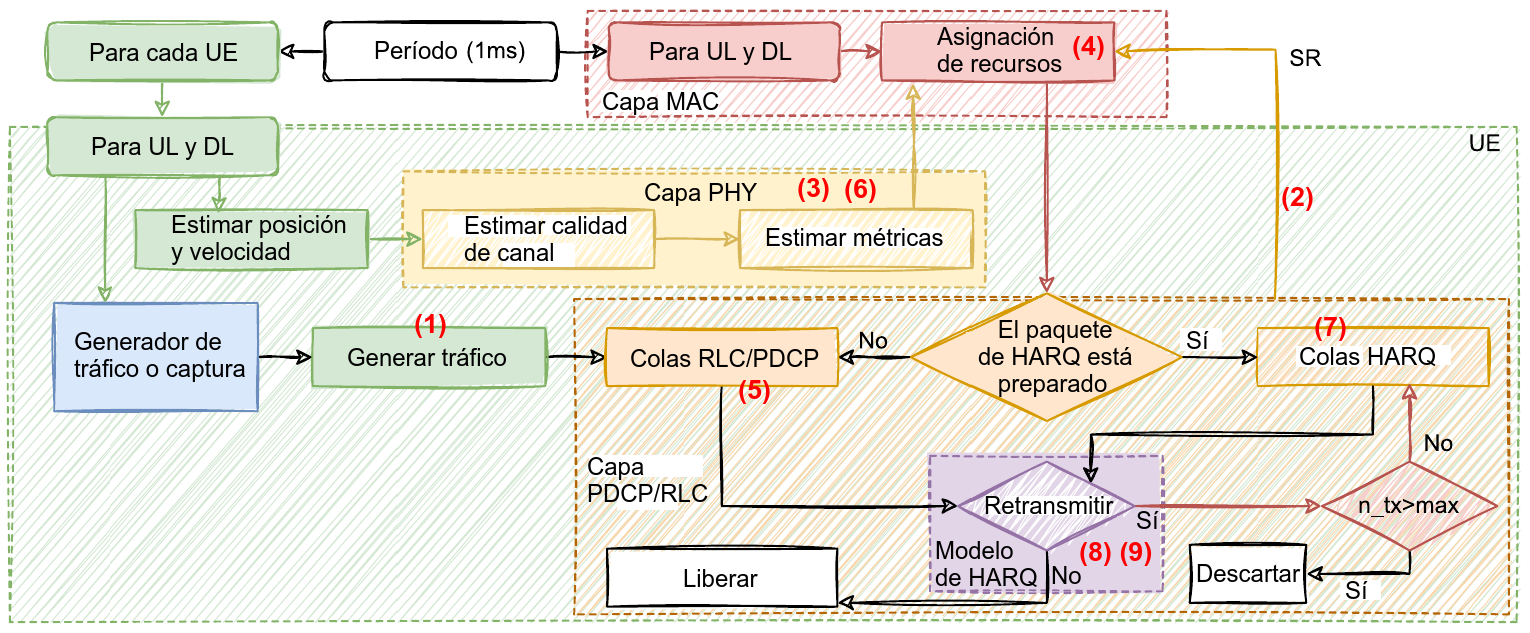
\includegraphics[scale=0.35]{imagenes/fikore_paper/fikore_paper2-001_es_pasos.png}}
\end{figure}

\subsection{Capacidades}

Como hemos descrito, el emulador representa las principales funciones de la NR (PHY, MAC, PDCP/RLC).
\textit{FikoRE} emula o simula (en función de si el tráfico es tomado de tramas reales o de si es simulado) la conexión de una o varias entidades de UE a una entidad de BS.
Todos los elementos de la interfaz de radio que median entre el UE y la BS (véase la figura 2.5) quedan representados.

Esto permite plantear despliegues completos y realistas que se ajustan a casos de uso de gran interés.
En la siguiente figura se puede ver un ejemplo:

\begin{figure}[H]
	{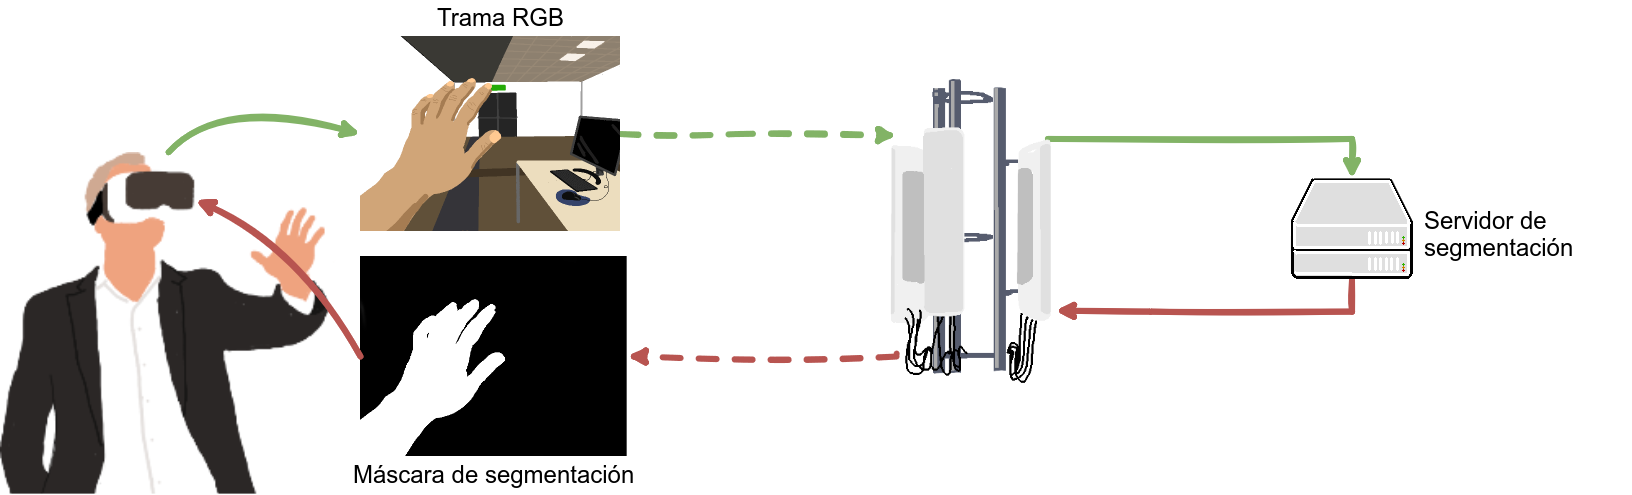
\includegraphics[scale=0.3]{imagenes/fikore_doc/figures/XROffloadingExample_es.png}}
	\ffigbox[\FBwidth] {
	\caption[Ejemplo con \textit{FikoRE} (I)]{Caso de uso: comunicación de un dispositivo HMD (\textit{Head Mounted Display}) equipado con cámara frontal con un servidor de segmentación.
	El servidor computa una máscara de segmentación a partir de la imagen tomada con la cámara frontal y la envía al usuario del HMD.
	La conexión entre los dos elementos finales se realiza mediante una red de 5G.

	(Arriba): Esquema para un despliegue real que permita el caso de uso.

	(Abajo): Esquema del mismo despliegue emulado con \textit{FikoRE}.

	Fuente: \cite{RefWorks:7}}
	}
	{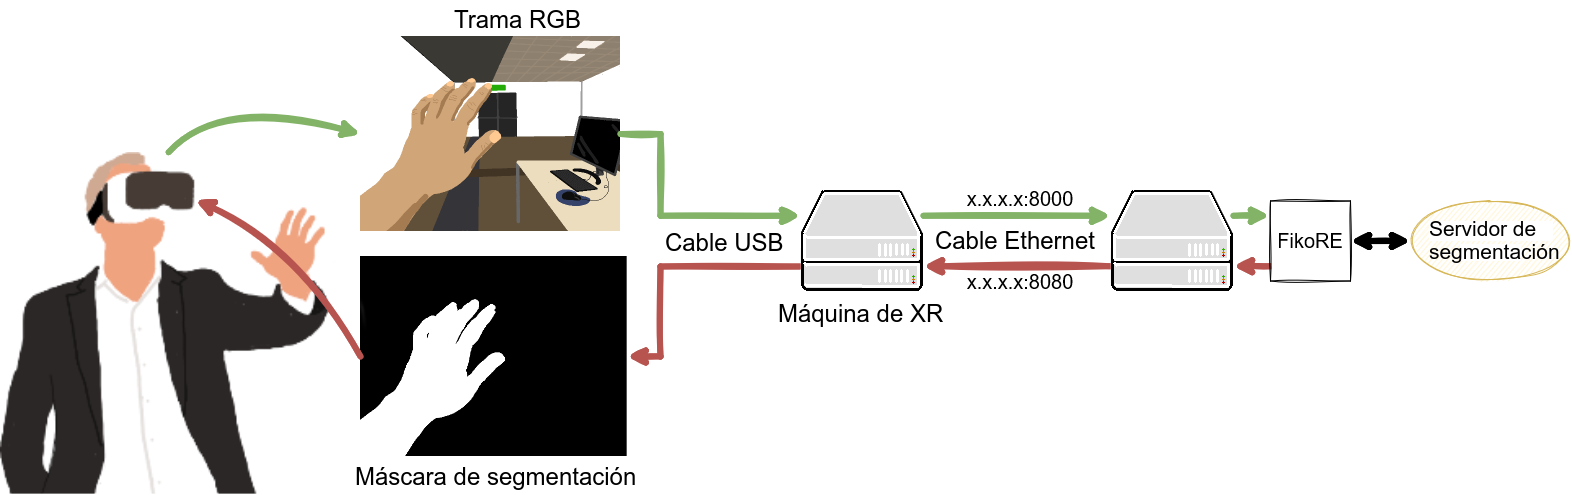
\includegraphics[scale=0.3]{imagenes/fikore_doc/figures/XROffloadingSetup_es.png}}
\end{figure}

Es importante discernir el lugar del emulador en el panorama del desarrollo de los sistemas 5G y de las aplicaciones que hacen uso de éstos.
\textit{FikoRE} permite simular una celda de 5G, lo que es suficiente para estudiar muchos casos de uso simples que hacen uso de las funcionalidades de los sistemas de 5G.
En cambio, quedan fuera de su alcance las funcionalidades que requieren la interacción con otras celdas o requieran la comunicación con el núcleo de red
(redes heterogéneas, nodos repetidores, transmisión multipunto coordinada, etc.).

\begin{figure}[H]
	\ffigbox[\FBwidth] {
	\caption[Ejemplo con \textit{FikoRE} (II)]{Gráfica de la trayectoria seguida por varios UE en una simulación.
	\textit{FikoRE} permite simular una celda de 5G.
	}
	}
	{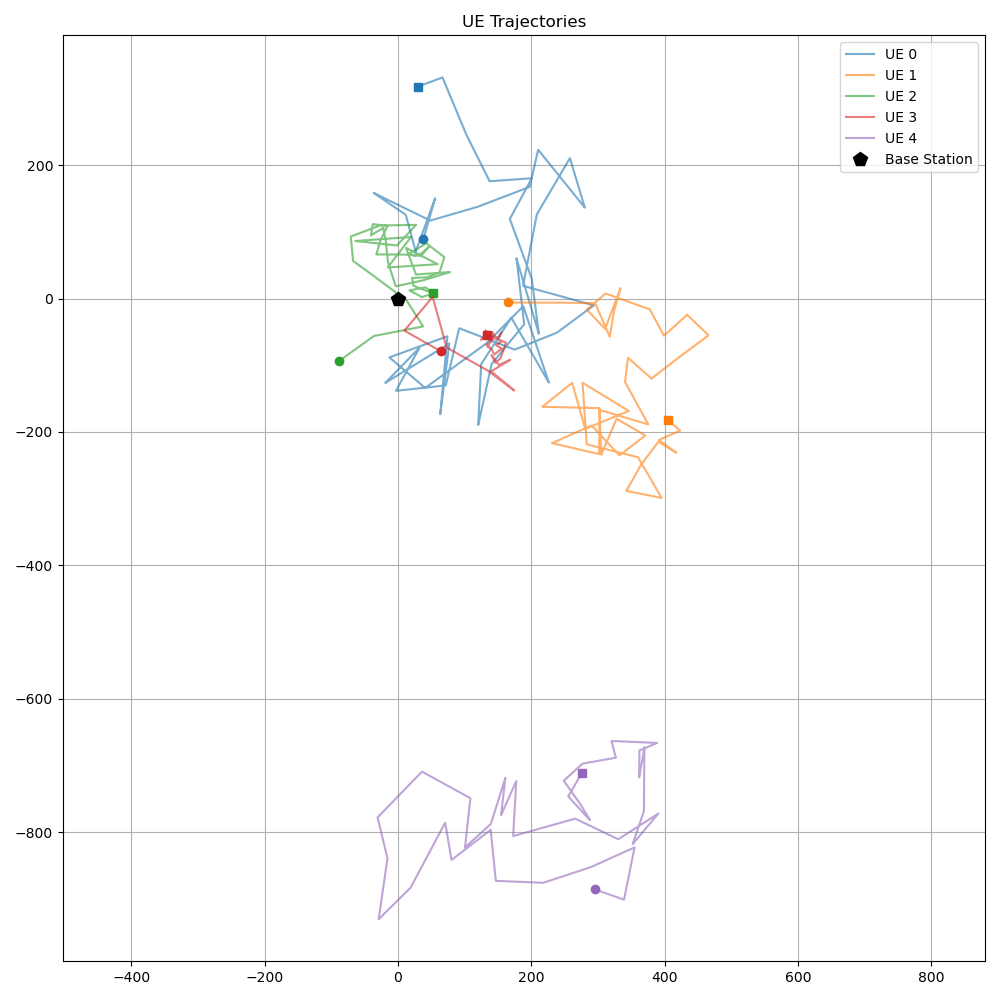
\includegraphics[scale=0.5]{../computos_y_graficas/pruebas/2_28_19_1_40/ue/trajectory.png}}
\end{figure}

El emulador representa y permite configurar muchas características de las redes móviles \cite{RefWorks:5, RefWorks:3, RefWorks:7, RefWorks:100}.
Para más detalle sobre su configuración y análisis, véase el \textbf{anexo A}.
A continuación, se resumen:
\begin{itemize}
\item Fenómenos de la transmisión inalámbrica:
ruido, interferencia, atenuación, desvanecimiento lento, desvanecimiento rápido.
\item Sistema celular:
el emulador representa la interferencia producida por otras células.
\item Procesado de señal:
eso incluye la modulación OFDM y las técnicas multiantena.
\item Otras técnicas avanzadas:
HARQ, planificación de paquetes, adaptación de enlace, agregación de portadoras.
\end{itemize}

\section{Detalles particulares}

En esta sección se resaltan las características que pueden tener repercusión en la la precisión, la exactitud y, en general, la calidad de una simulación de algún caso de uso particular.

\subsection{Validación del funcionamiento}

En las fuentes se describen varios experimentos para probar las capacidades del emulador.
El emulador sólo ha sido validado en experimentos en los que el UE era estático y había línea de visión (\textit{Line of Sight}, LOS). \cite{RefWorks:5, RefWorks:3}
Algunos comportamientos no se detallan, por lo que será necesario validarlos.

\subsection{Relativas a la ejecución}

\subsubsection{Duplicidad de instancias (UL/DL)}

Todos los módulos se instancian para cada dirección de transmisión, esto es, el enlace descendente (DL) y el enlace ascendente (UL).
Así, en el UE hay una instancia de los búferes de IP, HARQ y \textit{Packet Release} para cada dirección (UL/DL). \cite{RefWorks:5, RefWorks:3, RefWorks:7}

\begin{figure}[H]
	\ffigbox[\FBwidth] {
	\caption[Instancias en \textit{FikoRE}]{Duplicidad de instancias en \textit{FikoRE}.
	Se pueden apreciar las instancias para cada dirección (UL/DL) para cada UE y para la capa MAC.

	Fuente: \cite{RefWorks:7}}
	}
	{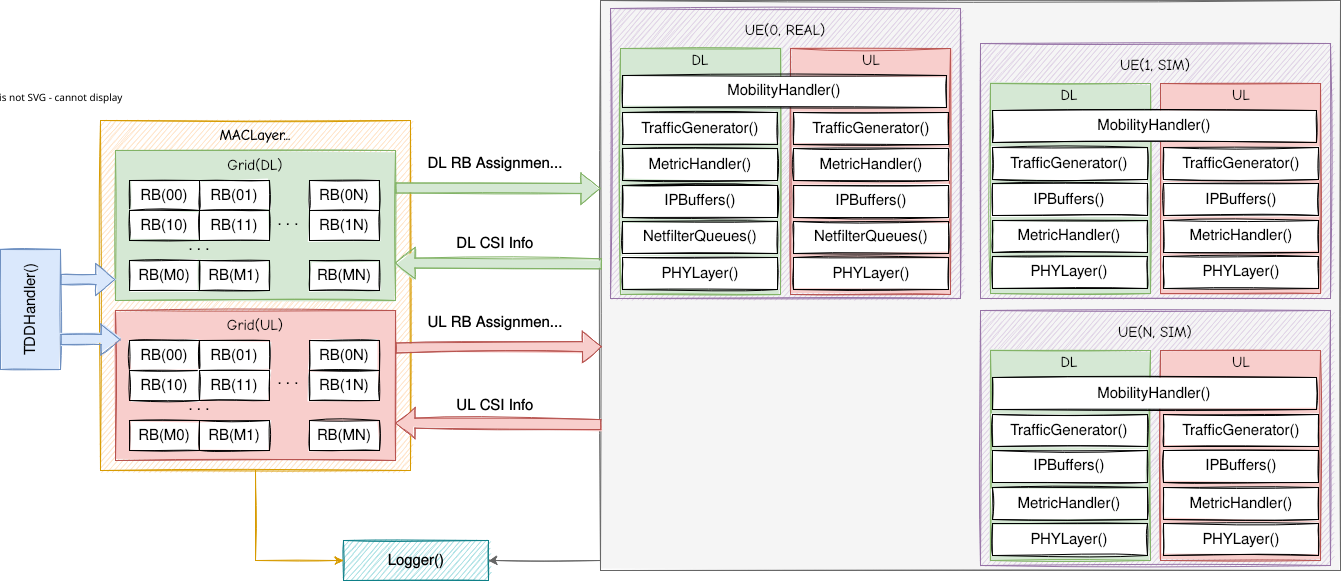
\includegraphics[scale=0.4]{imagenes/fikore_doc/figures/EmuImplementation.png}}
\end{figure}

\subsubsection{Sincronía de la ejecución}

Los pasos descritos en el epígrafe \textit{Flujo de información} se ejecutan una vez en cada período de ejecución con la tasa impuesta por el usuario (por defecto, el período es de 1 ms).
Existen dos procesos principales que se ejecutan consecutivamente: el de los UE y el de la capa MAC (gNB).
\cite{RefWorks:5, RefWorks:3, RefWorks:7}

\begin{enumerate}
\item Se lanza el proceso de la capa MAC en varios hilos y se espera hasta que todos terminen su tarea.
\item Se lanza el de los UE en varios hilos y se espera hasta que todos terminen su tarea.
\item Se espera hasta que termine el período de ejecución.
Si no es posible completar las tareas dentro del límite impuesto, el programa finaliza su ejecución.
\end{enumerate}

El límite para el cumplimiento de esta velocidad de ejecución es estricto, ya que permite la correcta sincronización entre el emulador y el manejo del tráfico IP.

\subsubsection{Módulo \textit{Netfilter Queue}}

Para manejar tráfico IP real, se usa el módulo \textit{Netfilter Queue} (NQ).
NQ es una API del espacio de usuario de \textit{Linux} que permite acceder a los paquetes que han sito encolados por el cortafuegos (\textit{firewall}).
\cite{RefWorks:5, RefWorks:3, RefWorks:7}

\subsection{Asunciones en la simulación}

\subsubsection{Tasa de asignación de recursos de radio}

En la gNB (capa MAC), la asignación de recursos de radio se lleva a cabo una vez por cada período de ejecución (por defecto, 1 ms) del programa en lugar de cada \textit{slot}, como hacen otros emuladores.
Teniéndose en cuenta que un \textit{slot} dura, dependiendo de la numerología, 1 ms o menos,
esta simplificación reduce la exactitud de la representación de la capa MAC en los casos en que el UE se desplace a gran velocidad ya que el tiempo de coherencia puede ser inferior al período elegido por el usuario y en un despliegue real se realizaría a una tasa mayor,
pero permite reducir las cabeceras de procesado e incrementar la escalabilidad del emulador.
\cite{RefWorks:3, RefWorks:7}

\subsubsection{Ruido e interferencia}

En el UE, en la simulación de PHY, el emulador estima el ruido y la interferencia al comienzo de una simulación y estos valores permanecen constantes.
Esta simplificación anula la varianza de esos dos elementos e impide apreciar, a lo largo de una simulación, sus efectos cambiantes,
pero permite reducir las cabeceras de modelado e incrementar la escalabilidad del emulador.
\cite{RefWorks:5, RefWorks:3, RefWorks:7}

\subsubsection{Velocidad máxima en \textit{Uma}}

Mediante simulaciones, se ha observado que la máxima velocidad que el UE puede tomar en celdas urbanas (\textit{Uma}) es \textasciitilde 0.8 m/s.
No es posible simular UE a gran velocidad en un entorno urbano.
%\cite{RefWorks:100}

%\subsubsection{Procesos de CQI}
%
%En el UE, en la simulación de PHY, el efecto del canal en la transmisión, que finalmente eleva la tasa de error, se estima en paralelo a los parámetros CQI. \cite{RefWorks:100}

\subsubsection{Modelos de canal}

En el UE, en la simulación de PHY, los efectos durante la transmisión inalámbrica que se consideran son los que aparecen en la especificación 3GPP 38.901.
\cite{RefWorks:5, RefWorks:3, RefWorks:7}

\begin{figure}[H]
	\ffigbox[\FBwidth] {
	\caption[Modelos de canal en \textit{FikoRE} (I)]{Esquema con los modelos usados por \textit{FikoRE} para estimar el canal de propagación.
	Se pueden ver la estimación de los parámetros dependientes del canal (SINR, MCS, RI), la probabilidad de línea de visión (LOS), de las pérdidas por propagación (\textit{pathloss}), del desvanecimiento (\textit{shadowing}), del ruido (\textit{noise}) y de la interferencia (\textit{interference}).

	Fuente: \cite{RefWorks:7}}
	}
	{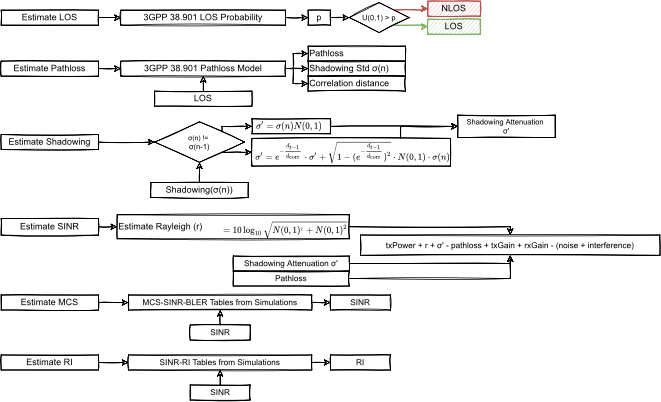
\includegraphics[scale=0.8]{imagenes/fikore_doc/figures/ModelsPHY.png}}
\end{figure}

Se usan los modelos del apartado \textit{Pathloss, LOS probability and penetration modelling}.
Estos modelos tienen en cuenta diversos efectos de la transmisión inalámbrica (atenuación, desvanecimiento lento, desvanecimiento rápido),
pero los convierten en fenómenos con una forma estadística que se aplican de la misma manera para dos UE o dos gNB distintos
(consideramos distintos un UE real A que se comunica con una gNB A en una ciudad A y un UE real B que se comunica con una gNB B en una ciudad B),
sólo atendiendo a las variables de entrada que el modelo considere para estimar el canal de propagación.
\cite{RefWorks:46}

Por ejemplo:
para representar un entorno urbano no se usa ningún plano urbano real,
sino que el reflejo de la señal electromagnética en los edificios u otros obstáculos es representado por un modelo que,
en función de diversas variables de entrada (distancia del UE a la gNB, anchura de la calle, altura de la gNB, etc.),
estima los parámetros que afectarán a la calidad de la transmisión (SINR, latencia, etc.).

\begin{figure}[H]
	{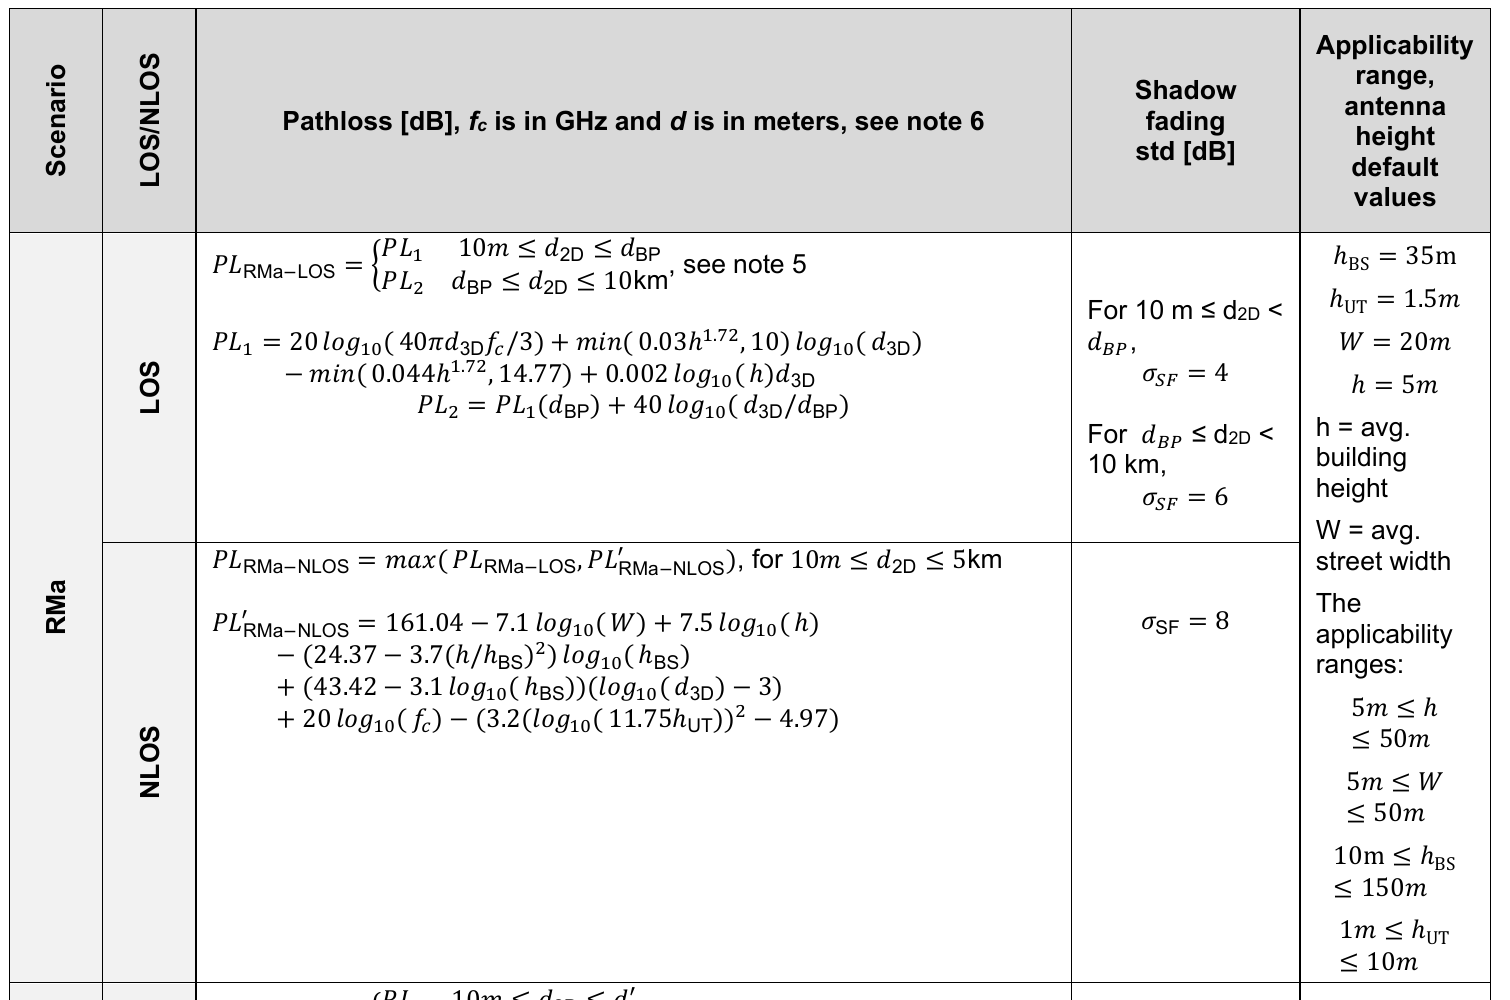
\includegraphics[scale=0.32]{imagenes/3gpp_ts_38901/TS_38901_extracto_1.png}}
	\ffigbox[\FBwidth] {
	\caption[Modelos de canal en \textit{FikoRE} (II)]{Extractos de la especificación 3GPP 38.901.

	(Arriba): Tabla con modelos para el cálculo de la atenuación (\textit{pathloss}) en los casos con línea de visión (\textit{Line-Of-Sight}, LOS) o sin ella (\textit{Non-Line-Of-Sight}, NLOS) en una celda rural (\textit{Rural Macro}, RMa).

	(Abajo): Tabla con modelos para el cálculo de la probabilidad de línea de visión en una celda rural, una microcelda urbana (\textit{Urban Micro}, UMi) y una macrocelda urbana (\textit{Urban Macro}, UMa).

	\textit{FikoRE} modela un mismo entorno de la misma manera para todos los UE atendiendo a las precisiones indicadas en los modelos.

	Fuente: \cite{RefWorks:46}}
	}
	{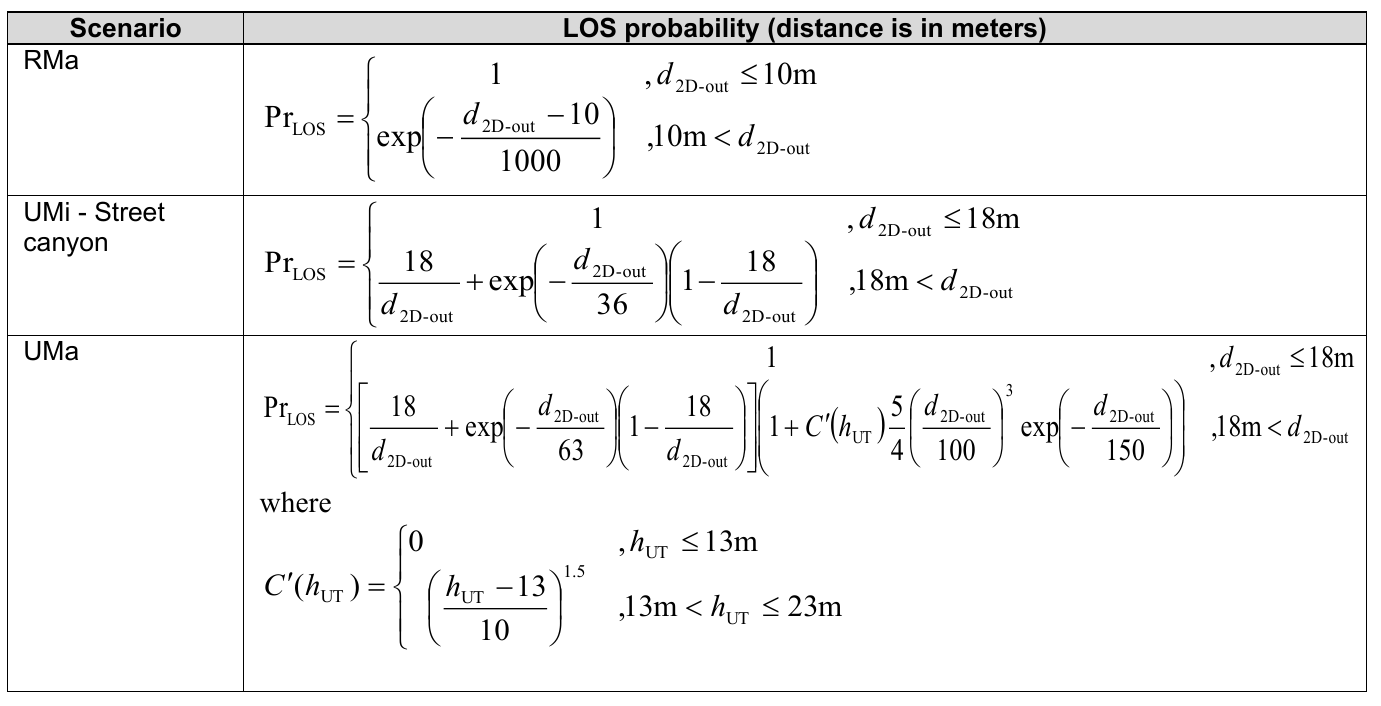
\includegraphics[scale=0.35]{imagenes/3gpp_ts_38901/TS_38901_extracto_2.png}}
\end{figure}

Esta no es la única manera de tratar el canal de propagación, hay otros trabajos relevantes de modelado del canal de propagación (\textit{IEEE}, \textit{COST}, etc.) que pueden servir en casos concretos.
Los proveedores de equipo de telecomunicaciones (\textit{Nokia}, \textit{Ericsson}, \textit{Huawei}, etc.) pueden dar sus propias soluciones a esos casos concretos.
3GPP únicamente se limita a describir las características del canal que se debe estimar y las funciones que deben realizar con esa información las tecnologías de 5G en una especificación pública.
\cite{RefWorks:46}
De manera general, podemos afirmar que la simulación que \textit{FikoRE} hace del canal de propagación y el cálculo que hace de los valores CQI es peor que la que lleva a cabo un despliegue real profesional
pero lo suficientemente buena como para que sus resultados tengan valor en el desarrollo de aplicaciones de 5G.

\subsubsection{Efecto Doppler}

En el UE, en la simulación de PHY, es de gran interés atender la representación del efecto Doppler,
pues es un fenómeno determinante en muchos casos de uso de 5G, especialmente aquellos en los que el UE se desplaza a gran velocidad en entornos urbanos.
También, se relaciona con el multitrayecto al causar ambos efectos que el canal sea variante en el tiempo y la frecuencia.

En el código se usan, en src/phy\_layer/phy\_layer.cpp, los siguientes elementos \cite{RefWorks:100}:
\begin{itemize}
\item Variables: \textit{doppler\_f} (valor real, frecuencia Doppler), \textit{tc} (valor real, tiempo de coherencia), \textit{min\_sinr\_update} (valor real, período mínimo de actualización del valor de la SINR), \textit{sinr\_period} (valor real, período de actualización del valor de la SINR), \textit{update\_sinr} (booleano, actualizar o no el valor de la SINR).
\item Métodos: \textit{init\_update\_rates()} (calcular las tasas de actualización de los indicadores de calidad del canal), \textit{estimate\_channel\_state()} (actualizar los indicadores de calidad del canal).
\end{itemize}

Cuando el UE aumenta de velocidad, el efecto Doppler se intensifica:
el tiempo de coherencia se reduce, por lo que, para que la estimación del canal sea válida, se actualizan con mayor frecuencia el valor de SINR estimado,
esto es, el efecto Doppler no eleva directamente la tasa de error, pues no modifica la SINR, pero sí modifica la frecuencia con la que se actualiza la SINR y otros indicadores de calidad del canal.
Esto ocasiona que, para un período de asignación de recursos de radio (por defecto, 1 ms), se termine asignando uno u otro RB a uno u otro UE.
Por otro lado, el canal estimado también determina las probabilidades para HARQ. \cite{RefWorks:5, RefWorks:7}

\begin{figure}[H]
	{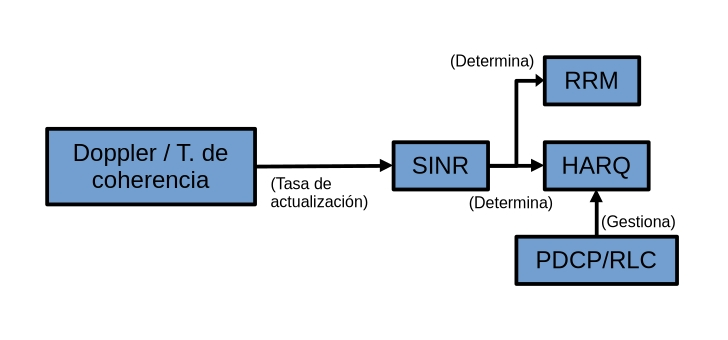
\includegraphics[scale=0.75]{imagenes/elaboracion_propia/ep_esquema_del_emulador.jpg}}
	\ffigbox[\FBwidth] {
	\caption[Efecto Doppler en \textit{FikoRE}]{Efecto Doppler en \textit{FikoRE}.

	(Arriba): Esquema de la relación entre el la estimación del efecto Doppler y el desarrollo de otras funciones.
	Al disminuir el tiempo de coherencia, aumenta la tasa de actualización de los indicadores de calidad del canal y, finalmente, afecta a los procesos de RRM y HARQ.
	Fuente: elaboración propia.

	(Abajo): Diagrama de flujo del cálculo de diversos valores.
	Se puede apreciar la relación entre el cálculo del tiempo de coherencia (\textit{corr\_time}) y el otros parámetros (SINR, MCS, RI).
	Fuente: \cite{RefWorks:7}}
	}
	{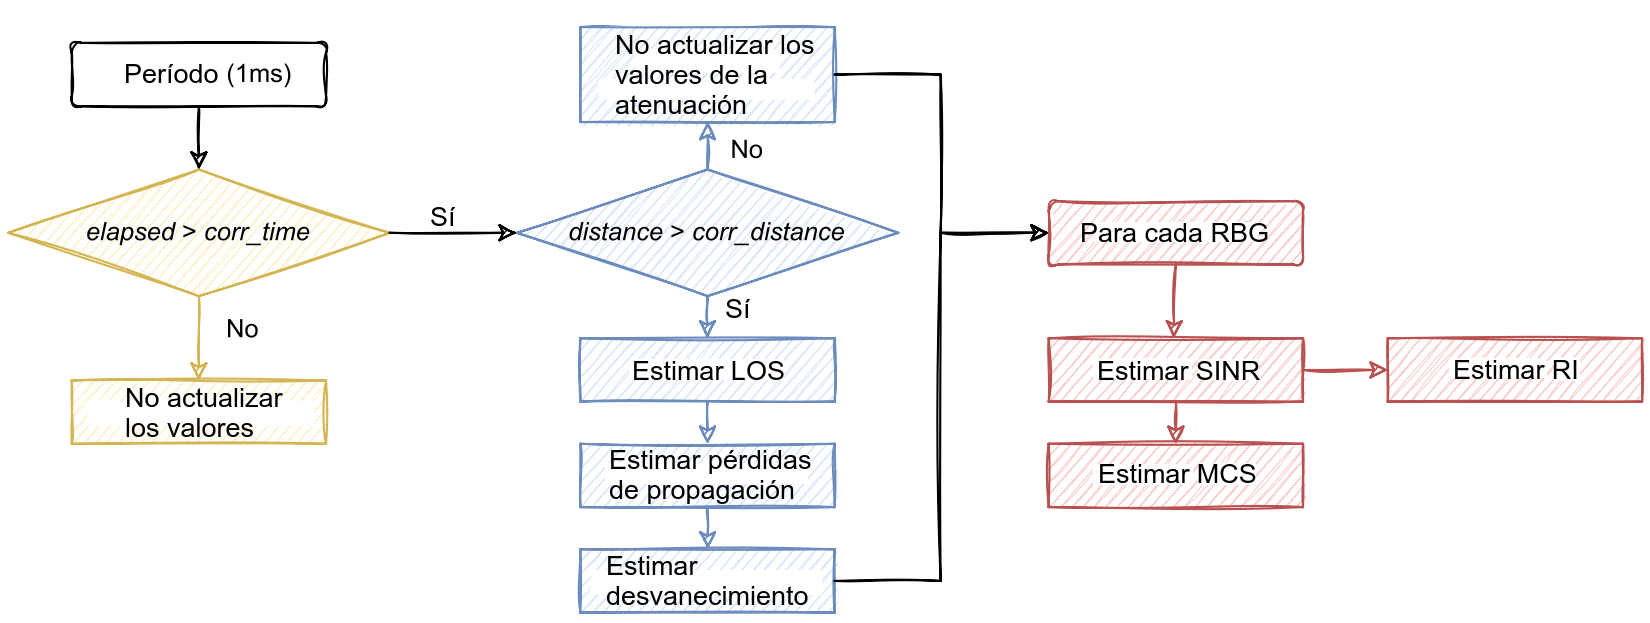
\includegraphics[scale=0.3]{imagenes/fikore_doc/figures/PHYFlow_es.png}}
\end{figure}

\paragraph{Validación}

Para validar el comportamiento en efecto Doppler, se han realizado varios conjuntos de simulaciones
(véase \textit{Validación - Efecto Doppler (conjunto 1)}, \textit{Validación - Efecto Doppler (conjunto 2)}, \textit{Validación - Efecto Doppler (conjunto 3)}, \textit{Validación - Efecto Doppler (conjunto 4)}, \textit{Validación - Efecto Doppler (conjunto 5)} en el anexo \textit{Simulaciones (metadatos)}).
En todos ellos se ha usado un UE que se alejaba de la gNB a la misma velocidad, pero en cada simulación del mismo conjunto a una velocidad mayor que la anterior simulación.
Las simulaciones eran breves (20 s) a fin de que el UE no se alejase tanto que la SINR fuese muy baja en las de velocidad mayor, haciendo imposible compararlas.
Los conjuntos se distinguen entre sí por algunos parámetros como la precisión temporal (\textit{period}), la tasa de reporte de datos (\textit{log\_freq}) o la tasa de actualización de parámetros de CQI (\textit{cqi\_period}, \textit{ri\_period}).

En todos los conjuntos, el uso de velocidades altas no supone un gran cambio significativo en la distribución de MCS, tasa binaria, RI, RSRP, SINR o CQI.
Esto se debe a que las técnicas de AMC permiten mantener las mismas tasas pese al incremento de velocidad.
Los cambios mínimos se pueden achacar a peculiaridades estadísticas (tráfico generado, trayectoria seguida, etc.) en del único UE simulado en cada simulación.

\begin{figure}[H]
	{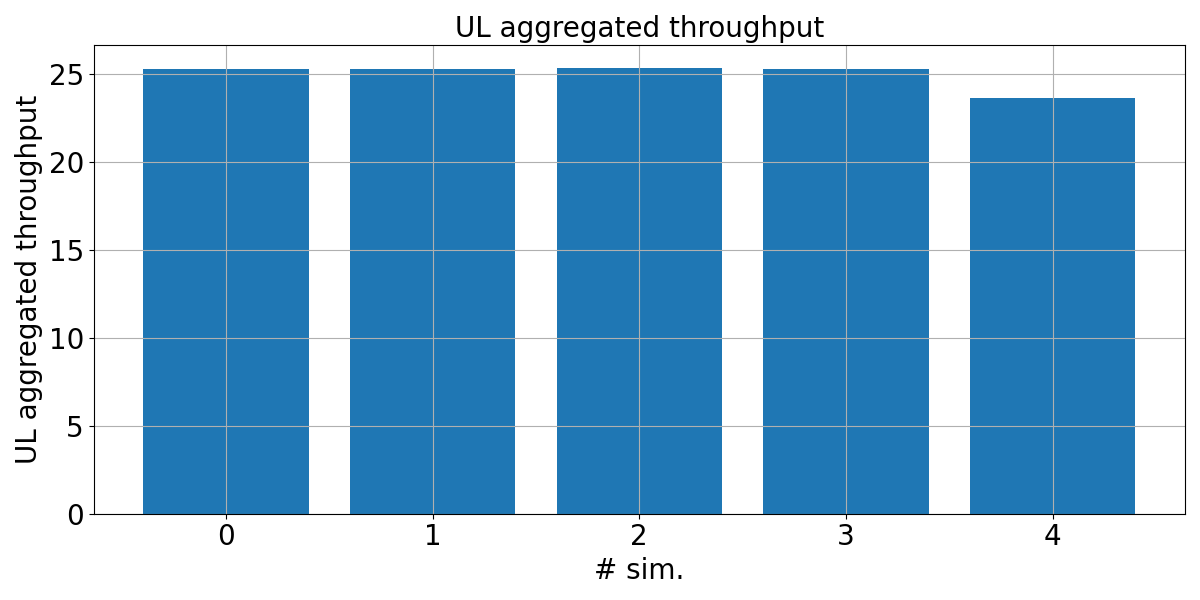
\includegraphics[scale=0.4]{../comparaciones/validacion_doppler_conjunto2/ue/ul_agg_throughput_multi_sim.png}}
	\ffigbox[\FBwidth] {
	\caption[Validación del efecto Doppler (I)]{Gráfica de \textit{Validación - Efecto Doppler (conjunto 2)}.

	Efecto en la tasa binaria promedio en el UE al elevar la velocidad del UE.

	(Arriba): Dirección UL.

	(Abajo): Dirección DL.}
	}
	{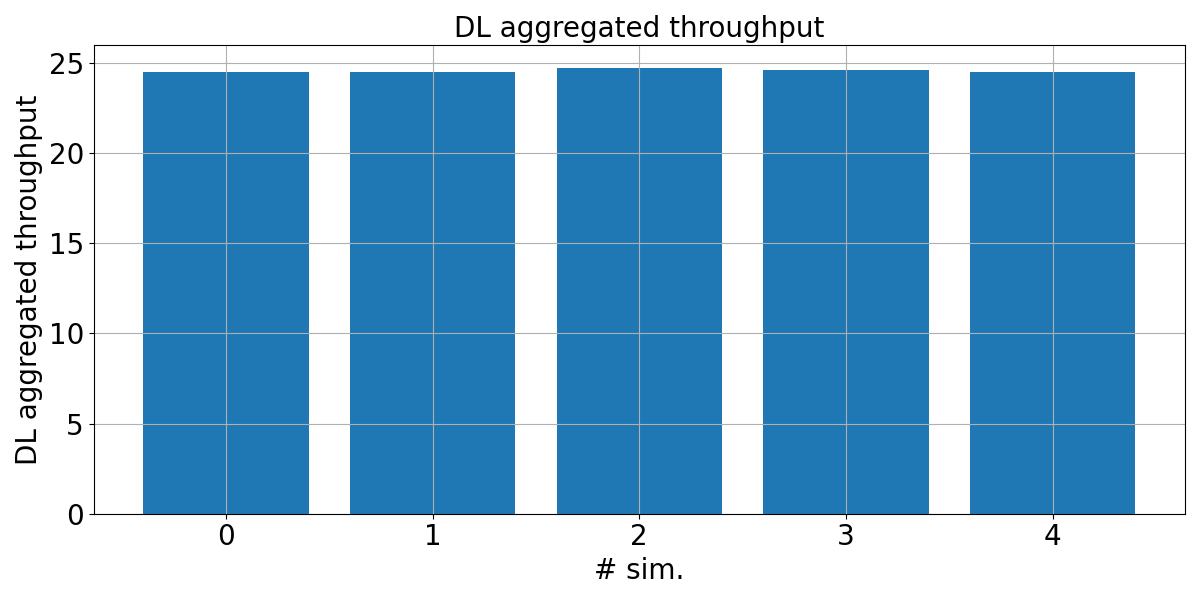
\includegraphics[scale=0.4]{../comparaciones/validacion_doppler_conjunto2/ue/dl_agg_throughput_multi_sim.png}}
\end{figure}

\begin{figure}[H]
	{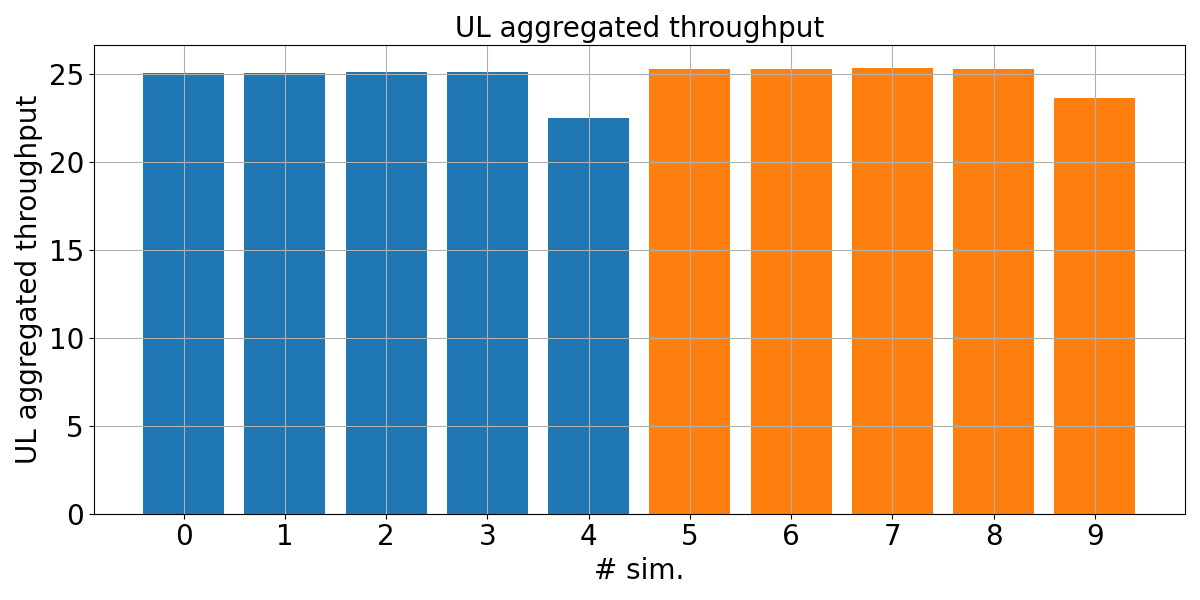
\includegraphics[scale=0.4]{../comparaciones/validacion_doppler_conjuntos_1_y_2/ue/ul_agg_throughput_multi_sim.png}}
	\ffigbox[\FBwidth] {
	\caption[Validación del efecto Doppler (II)]{Gráfica comparativa de \textit{Validación - Efecto Doppler (conjunto 1)} (azul) y \textit{Validación - Efecto Doppler (conjunto 2)} (naranja).

	Tasa binaria promedio.
	El conjunto 2 (mayor tasa de ejecución) tiene una tasa binaria ligeramente mayor por la misma justificación que se da en el epígrafe \textit{Granularidad temporal}.

	(Arriba): Dirección UL.

	(Abajo): Dirección DL.}
	}
	{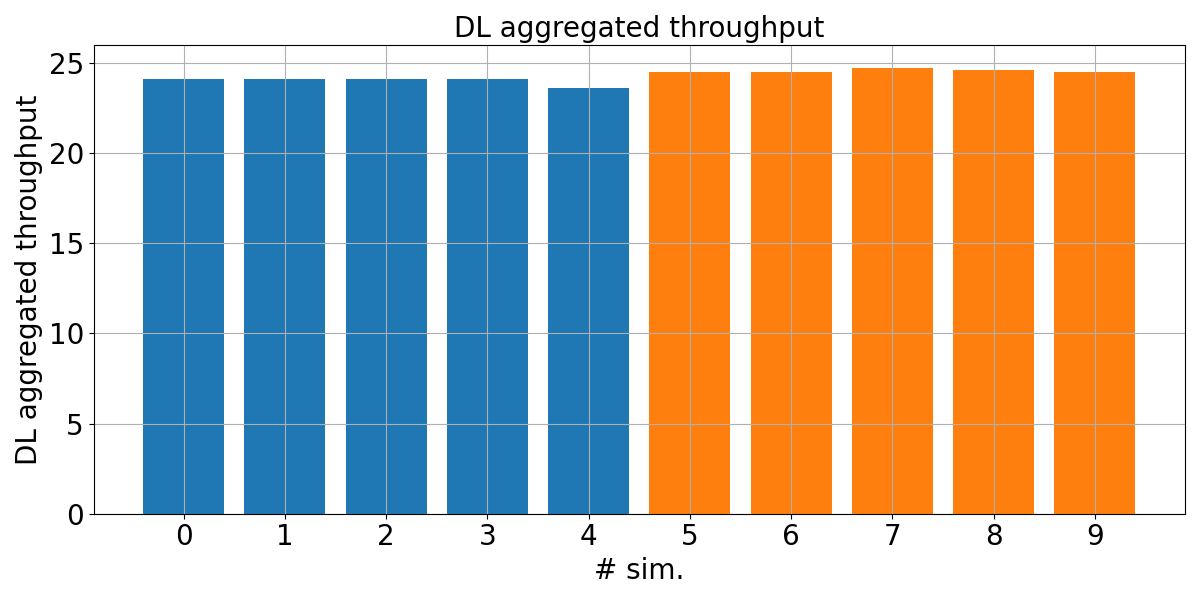
\includegraphics[scale=0.4]{../comparaciones/validacion_doppler_conjuntos_1_y_2/ue/dl_agg_throughput_multi_sim.png}}
\end{figure}

{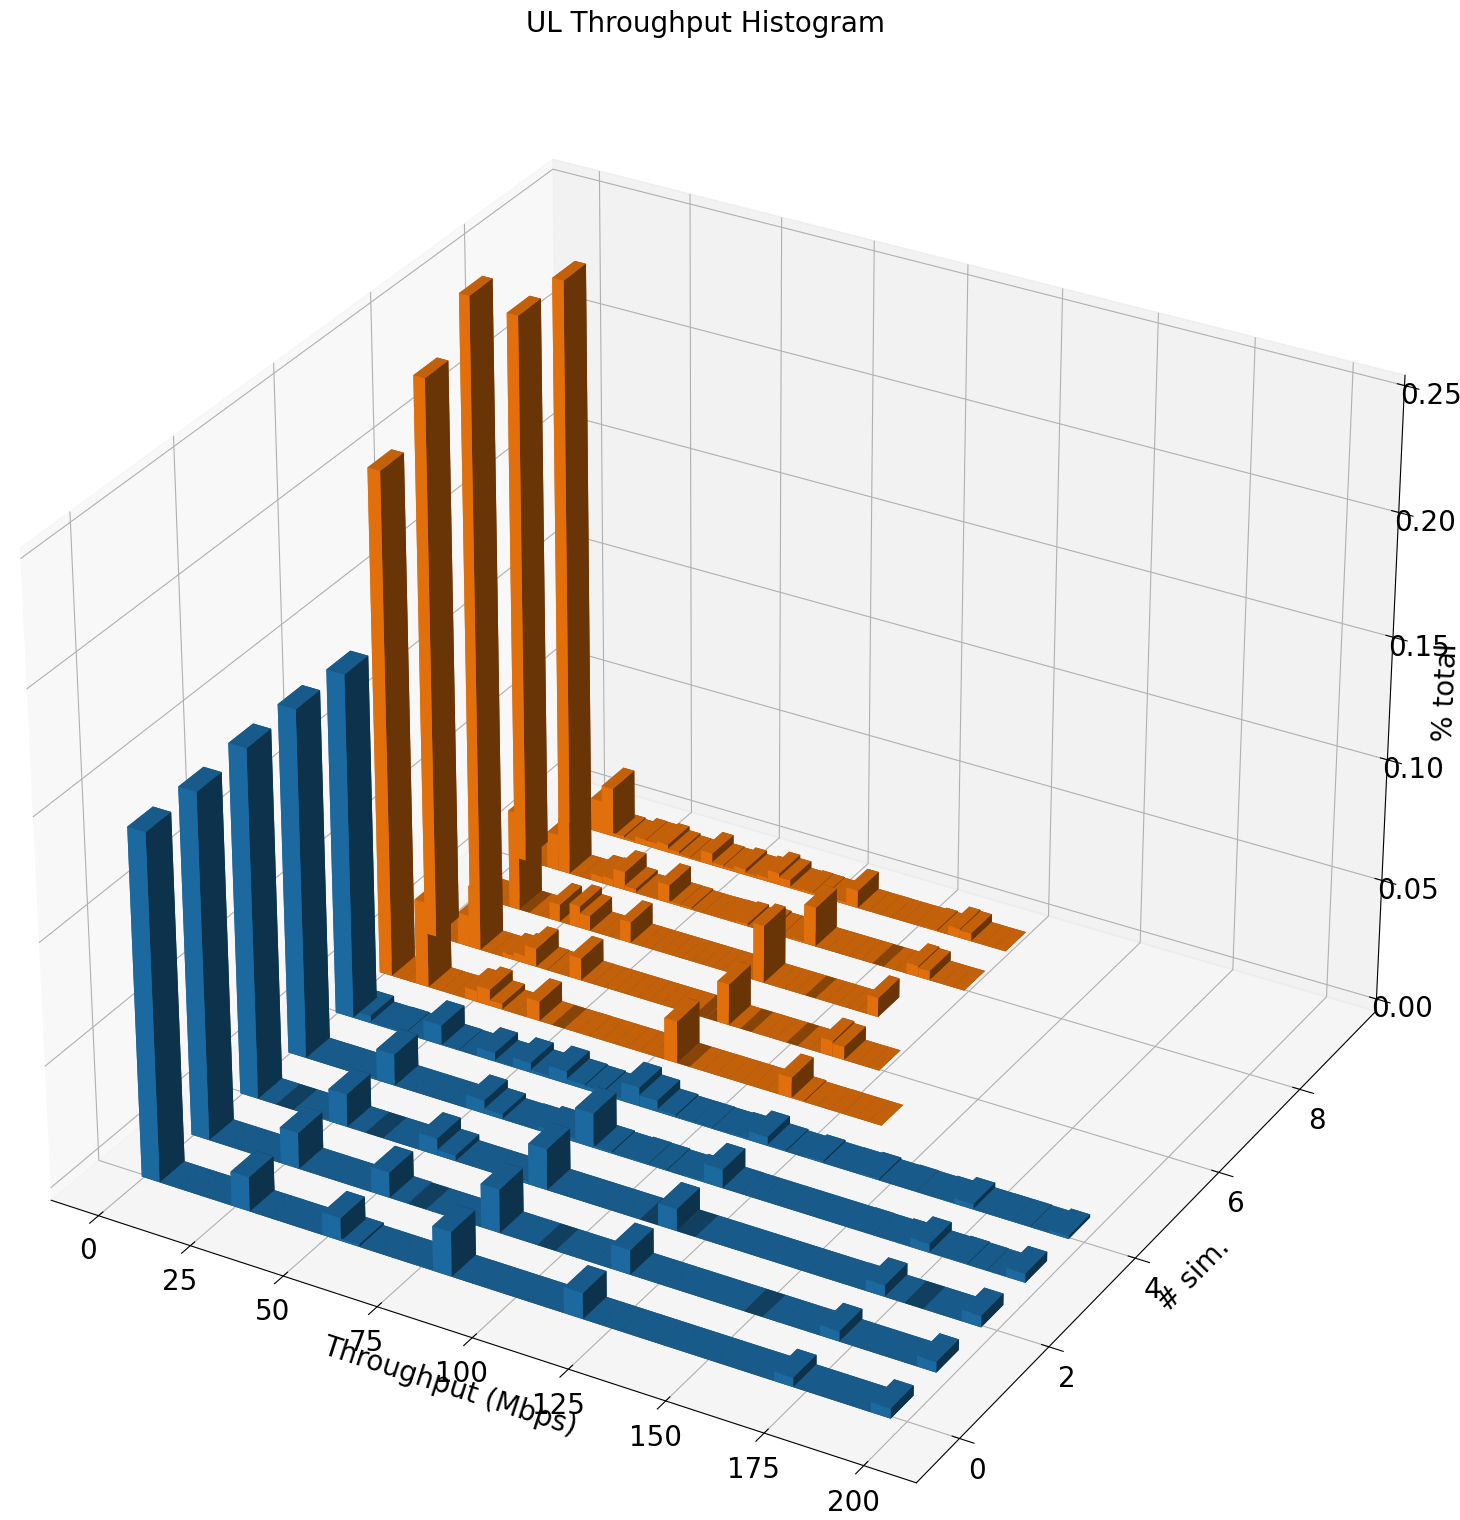
\includegraphics[scale=0.42]{../comparaciones/validacion_doppler_conjuntos_1_y_2/ue/rul_3d_hist_all_ue_multi.png_cropped.png}}

\begin{figure}[H]
	\ffigbox[\FBwidth] {
	\caption[Validación del efecto Doppler (III)]{Gráfica comparativa de \textit{Validación - Efecto Doppler (conjunto 1)} (azul) y \textit{Validación - Efecto Doppler (conjunto 2)} (naranja).

	Distribución de picos de tasa binaria.
	El conjunto 2 (mayor tasa de ejecución) tiene menos picos (solo se transmite en pequeñas cantidades) por la misma justificación que se da en el epígrafe \textit{Granularidad temporal}.

	(Arriba): Dirección UL.

	(Abajo): Dirección DL.}
	}
	{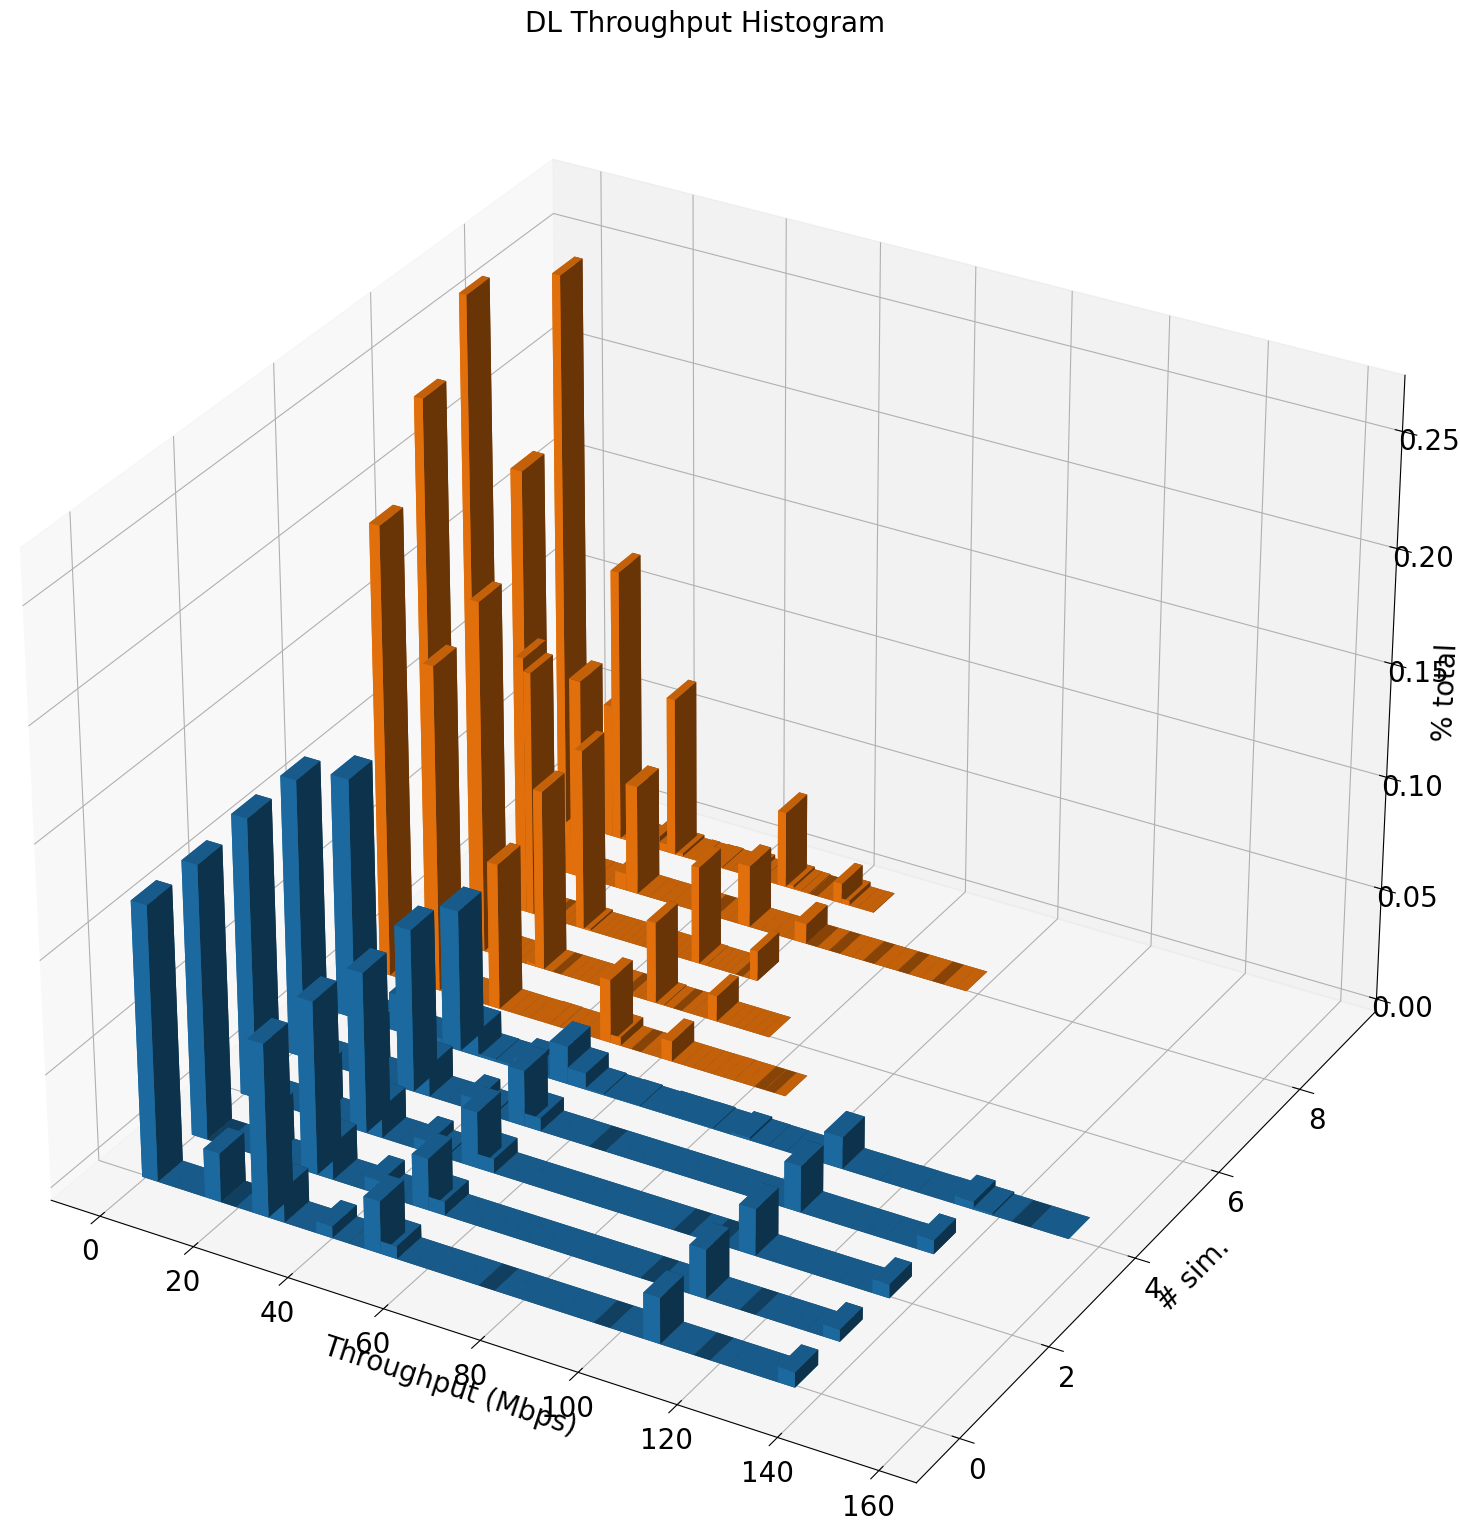
\includegraphics[scale=0.42]{../comparaciones/validacion_doppler_conjuntos_1_y_2/ue/rdl_3d_hist_all_ue_multi.png_cropped.png}}
\end{figure}

\subsubsection{Granularidad temporal}

En el UE, se ha comprobado el comportamiento al cambiar la precisión de la simulación (véase \textit{Validación - Granularidad} en el anexo \textit{Simulaciones (metadatos)}).
Se ha observado que el cálculo de los parámetros más indicativos de la simulación es posible en todos los casos,
se pueden comparar simulaciones llevadas a cabo con distintas tasas de ejecución.

La mayor diferencia es la comparación de tasa binaria.
Esto puede deberse a que la mayor tasa permite el paso de bloques de menores dimensiones, evitando que se den picos de mayor tasa.

\begin{figure}[H]
	\ffigbox[\FBwidth] {
	\caption[Validación de la granularidad (I)]{Efecto en la distribución de picos de tasa binaria al elevar la precisión temporal.
	Períodos de ejecución: 1 ms (azul), 0.5 ms (naranja), 0.1 ms (verde).}
	}
	{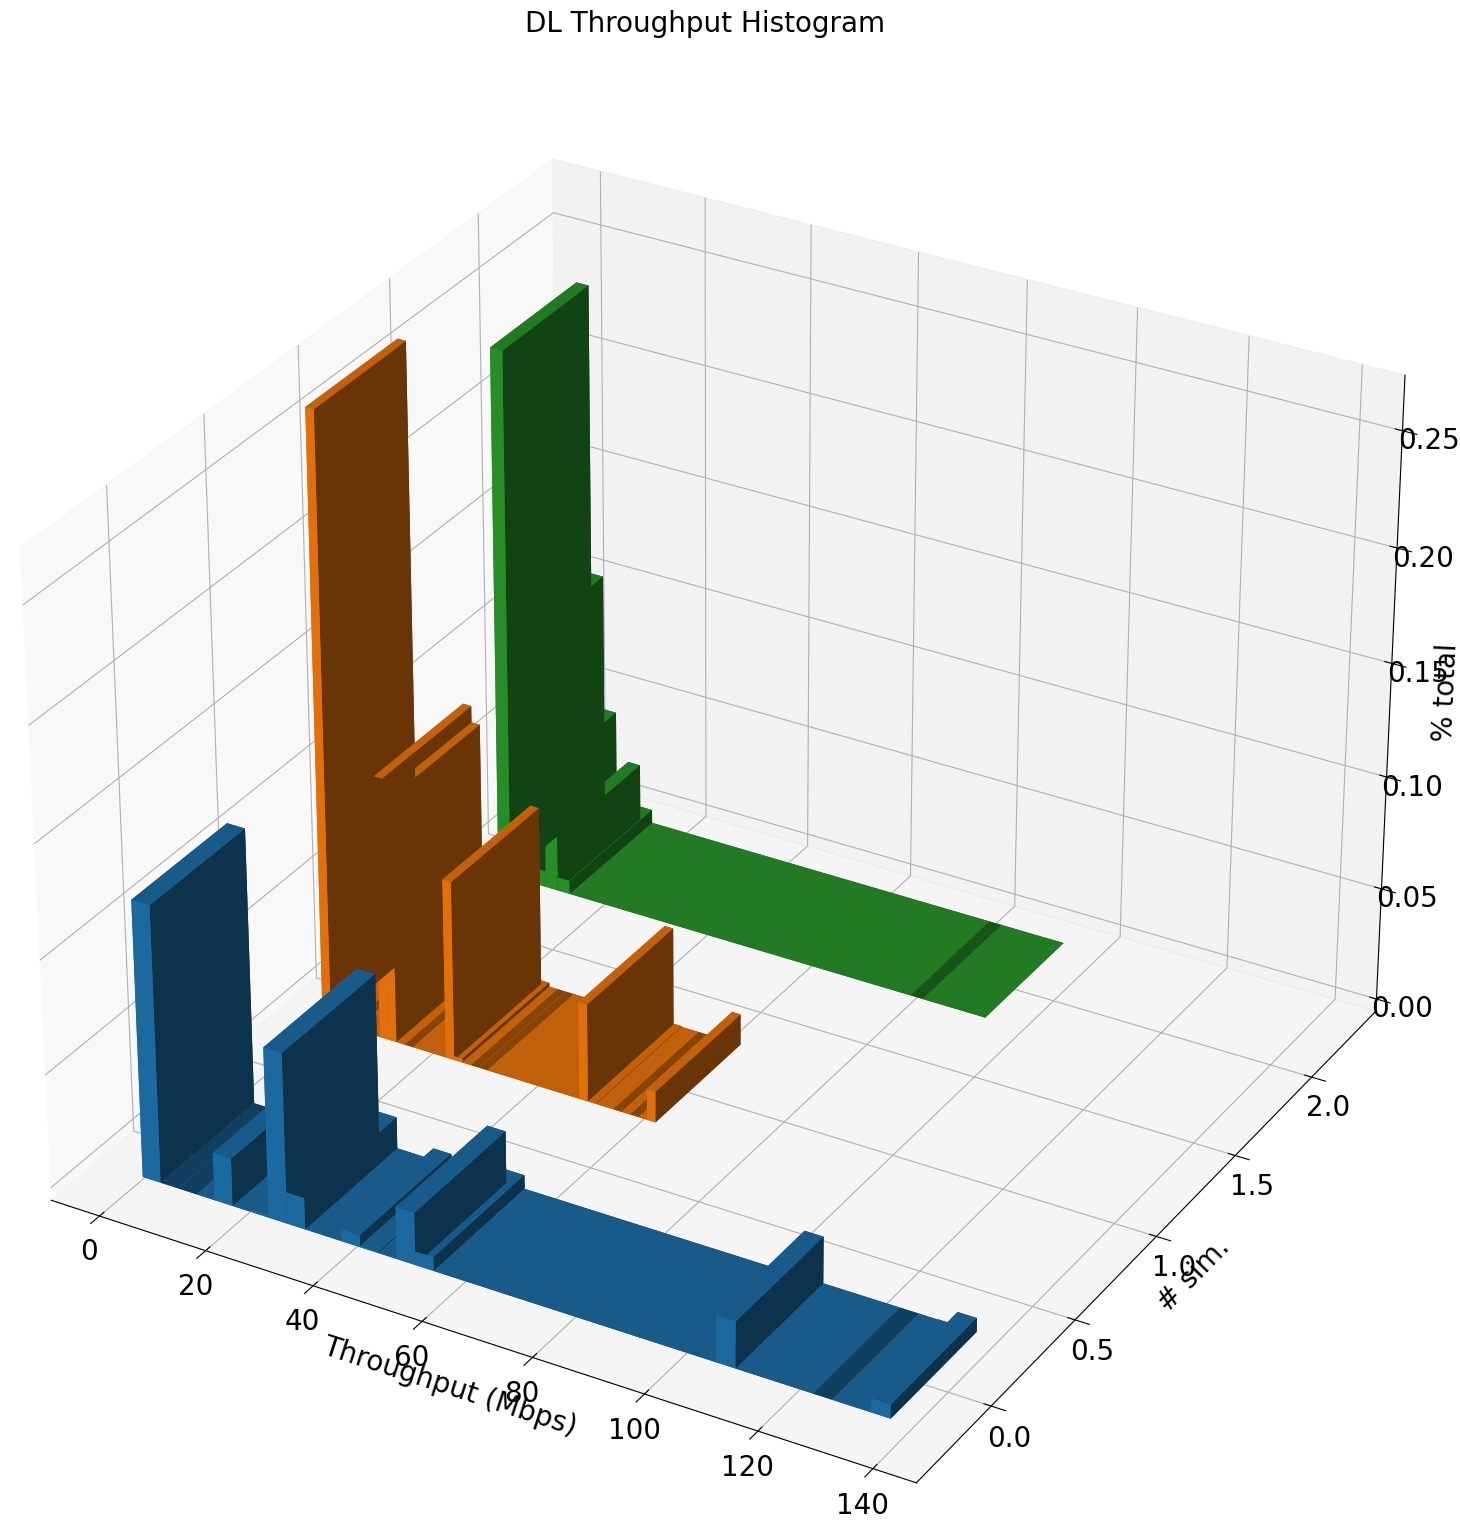
\includegraphics[scale=0.42]{../comparaciones/validacion_granularidad/ue/rdl_3d_hist_all_ue_multi.png_cropped.png}}
\end{figure}

\begin{figure}[H]
	\ffigbox[\FBwidth] {
	\caption[Validación de la granularidad (II)]{Efecto en la tasa binaria promedio en el UE al elevar la precisión temporal.
	Períodos de ejecución por orden: 1 ms, 0.5 ms, 0.1 ms.}
	}
	{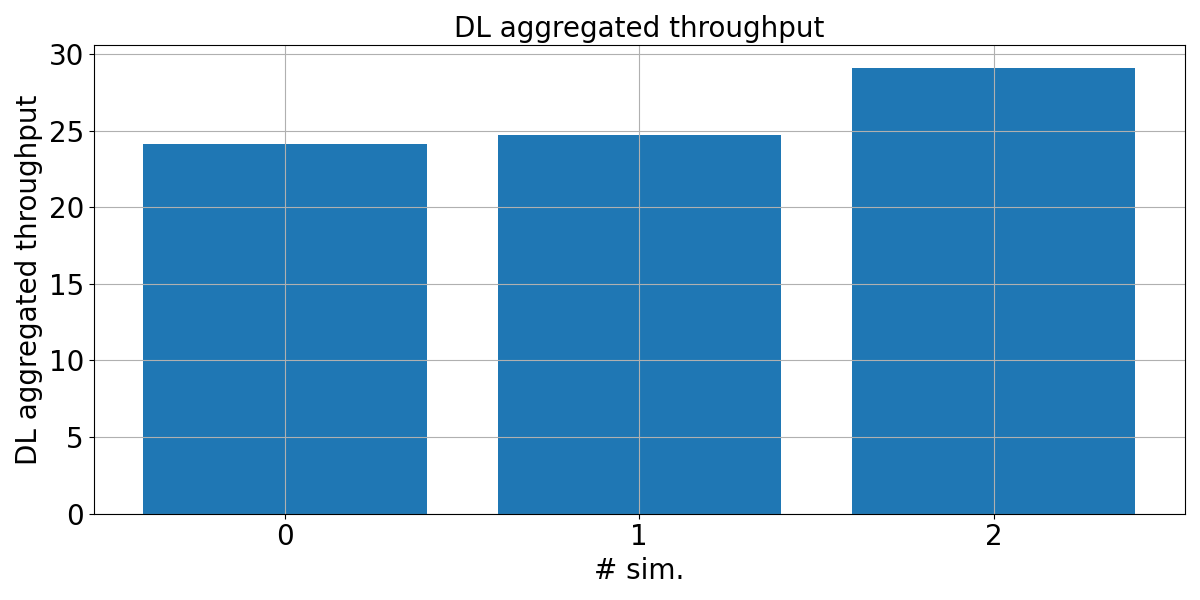
\includegraphics[scale=0.4]{../comparaciones/validacion_granularidad/ue/dl_agg_throughput_multi_sim.png}}
\end{figure}

\chapter{Caso de uso: planificación de paquetes (\textit{packet scheduling})}

\section{Introducción}

La planificación de paquetes es el proceso de asignación de los recursos de radio a los distintos UE de una red móvil a lo largo del tiempo.
En el sistema 5G es una funcionalidad implementada en la capa MAC y que lleva a cabo la gNB.
Coordina tanto el enlace ascendente como el descendente.
La planificación de paquetes es una funcionalidad muy determinante en las prestaciones de la red móvil.
\cite{RefWorks:73}

Para llevar a cabo la planificación de paquetes, la gNB se sirve de la información CQI, en la que los UE notifican el estado del canal de transmisión.
También se tienen en cuenta criterios cruciales para el buen funcionamiento, como la calidad de servicio (QoS), el estado de los búferes de datos de cada UE, etc.
La implementación del proceso se realiza sobre la descripción funcional del sistema 5G, identificando las entidades en juego (gNB, UE) y usando el sistema de interfaces y canales definido por los estándares.
\cite{RefWorks:73} \cite{RefWorks:26}
Se trata, pues, de un proceso complejo.

Distintas fuentes proponen distintos algoritmos en función del propósito.
Los algoritmos que se deben usar en la red no están especificados en los estándares de 3GPP, sino que se deja al juicio de los proveedores de equipo de red;
los únicos detalles especificados en los estándares son los procesos de la red de 5G sobre los que se apoya el proceso (canales y señales, CQI, etc.).
\cite{RefWorks:73}

\section{Proceso de asignación de recursos}

En lo que respecta al flujo de información, se puede resumir en los siguientes pasos \cite{RefWorks:73, RefWorks:26}:
1) los UE notifican a la gNB acerca del estado del canal mediante el mecanismo de CQI;
2) la gNB tiene en cuenta el estado de los canales de transmisión de cada UE y otros criterios, tras lo que lleva a cabo la asignación;
3) la asignación, tanto en UL como en DL, se notifica a los UE por medio de un canal físico, el PDCCH.
El período de asignación de recursos es tan minúsculo como de un \textit{slot}, que dura, dependiendo de la numerología, 1 ms o menos.
\cite{RefWorks:5, RefWorks:3}
La única diferencia entre los enlaces ascendente y descendente es que, mientras que para DL el planificador cuenta con la mayoría de información disponible, como el estado de los búferes de datos, para UL solo se cuenta con los informes del UE.

\begin{figure}[H]
	\ffigbox[\FBwidth] {
	\caption[Planificación de paquetes]{Modelo simplificado de un planificador de paquetes.

	Fuente: \cite{RefWorks:26}}
	}
	{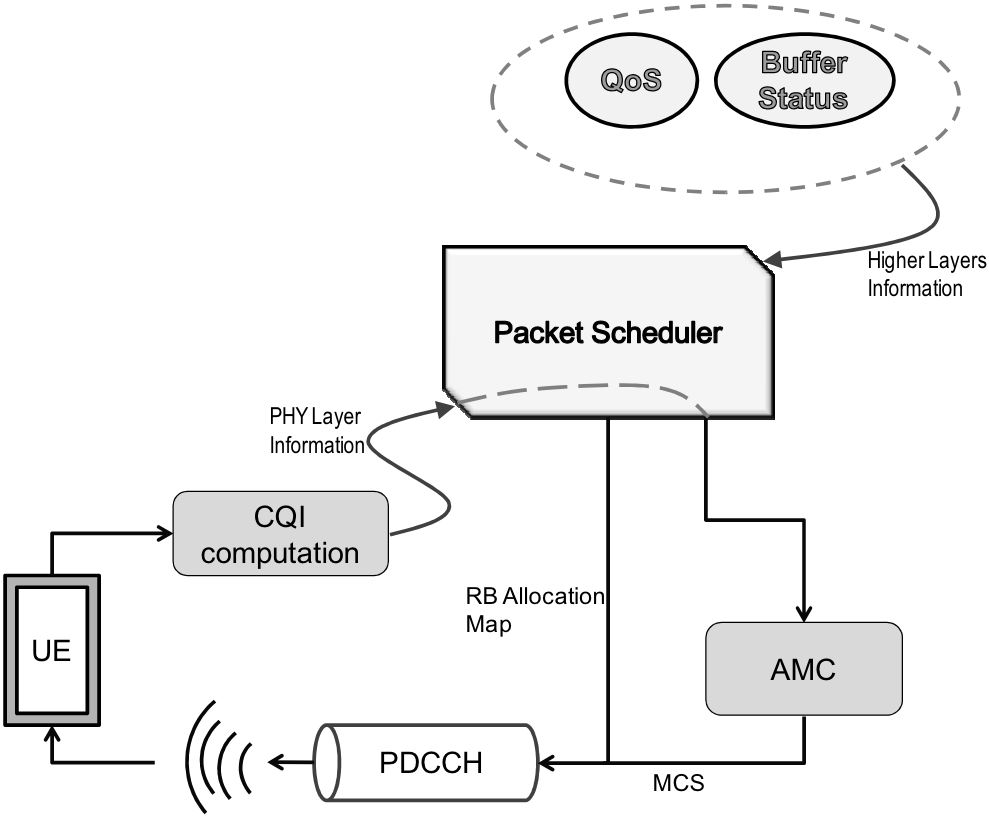
\includegraphics[scale=0.3]{imagenes/scheduling_italianos/scheduling_italianos-197.png}}
\end{figure}

El mecanismo que permite la asignación de recursos de radio combina dos funcionalidades \cite{RefWorks:73, RefWorks:26}:

\begin{itemize}
\item Por un lado, se usa AMC, que modifica el esquema de modulación usado (QPSK, 16-QAM, etc.) en cada PRB o en cada RBG dependiendo del estado del canal de transmisión y la cantidad de datos que se transmiten en UL ó DL.
\item La modulación OFDM, que divide los recursos de tiempo-frecuencia en una rejilla de recursos (PRB, RBG), permite asignar éstos a conveniencia.
Esto permite que, idealmente, no exista interferencia entre canales.
\end{itemize}

Para determinar a qué UE asignar un canal de radio se utiliza un método que culmina con el cómputo de una métrica para cada RB (\textit{Resource Block}, un PRB o un RBG);
el RB k-ésimo se asigna al UE j-ésimo si la métrica $m_{j, k}$ es superior a las demás \cite{RefWorks:26}:

$$
m_{j, k} = \max_i \lbrace m_{i, k} \rbrace
$$


El cómputo de la métrica se lleva a cabo teniendo en cuenta diversa información:
estado de las colas de transmisión, calidad del canal (CQI), historial de asignación de recursos de radio, estado de los búferes, calidad de servicio requerida (QoS). \cite{RefWorks:26}
El diseño del proceso de cálculo de las métricas tiene en cuenta diversos factores que se consideran valiosos en la red móvil:
complejidad frente escalabilidad \cite{RefWorks:26},
eficiencia espectral \cite{RefWorks:26, RefWorks:64},
justicia \cite{RefWorks:26, RefWorks:63, RefWorks:65},
provisión de QoS \cite{RefWorks:26}.
Se puede ver una lista exhaustiva en \cite{RefWorks:26}.

La incorporación de nuevas técnicas a las redes móviles,
como la agregación de portadoras (se modifica el dominio de frecuencias a asignar) o la multiplexación espacial mediante MIMO (dos usuarios de una misma celda dejan de compartir espacio, por lo que pueden compartir los mismos recursos de tiempo-frecuencia),
modifica los recursos de radio disponibles.
Las mismas métricas no sirven para dos despliegues que incorporen técnicas distintas.
\cite{RefWorks:26}
Es por ello que el diseño de la planificación de paquetes se debe adaptar a estos escenarios o el mismo debe hacerse de manera conjunta con el del resto de técnicas.

\section{Experimentos con el emulador}

La efectividad de esos algoritmos para cada caso puede ser estudiada mediante el emulador.

El emulador permite elegir entre siete métricas: FIFO (0), BET (1), EDF (2), LWDF (3), MT (4), RR (5), PF (6).
Se han introducido la métrica M-LWDF (7) siguiendo la expresión indicada en \cite{RefWorks:26}:

$$
m_{i, k}^{M-LWDF} = \alpha_i D_{HOL, i} \cdot \frac {d_{k}^i (t)} {\bar{R^i} (t-1)}
$$

\subsection{Comparación simple de métricas con \textit{FikoRE}}

Probamos la planificación de paquetes usando distintas métricas (RR, FIFO, BET, EDF, LWDF, MT, PF) en el escenario sencillo propuesto
(véase \textit{Caso de uso (VII): packet scheduling (iniciales)} en el anexo \textit{Simulaciones (metadatos)}).

\begin{figure}[H]
	{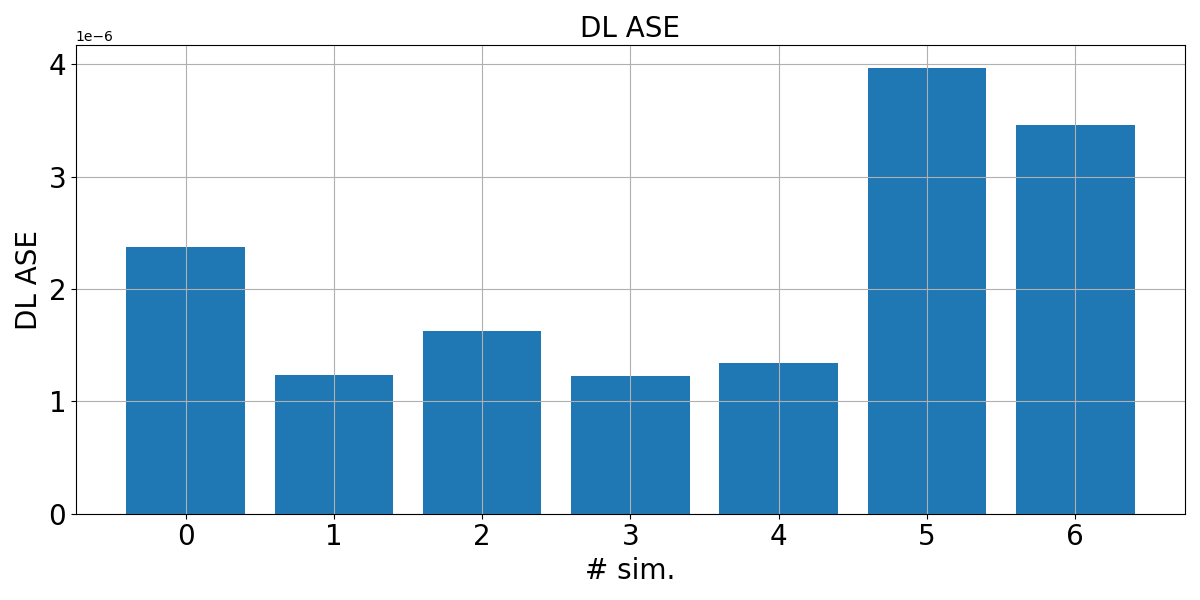
\includegraphics[scale=0.4]{../comparaciones/scheduling_iniciales/ue/dl_ase_multi_sim.png}}
	\ffigbox[\FBwidth] {
	\caption[Planificación de paquetes - Primer caso - ASE (I)]{Eficiencia espectral promedio con las distintas métricas.
	Las métricas por orden: RR, FIFO, BET, EDF, LWDF, MT, PF.

	(Arriba): Dirección DL.

	(Abajo): Dirección UL.}
	}
	{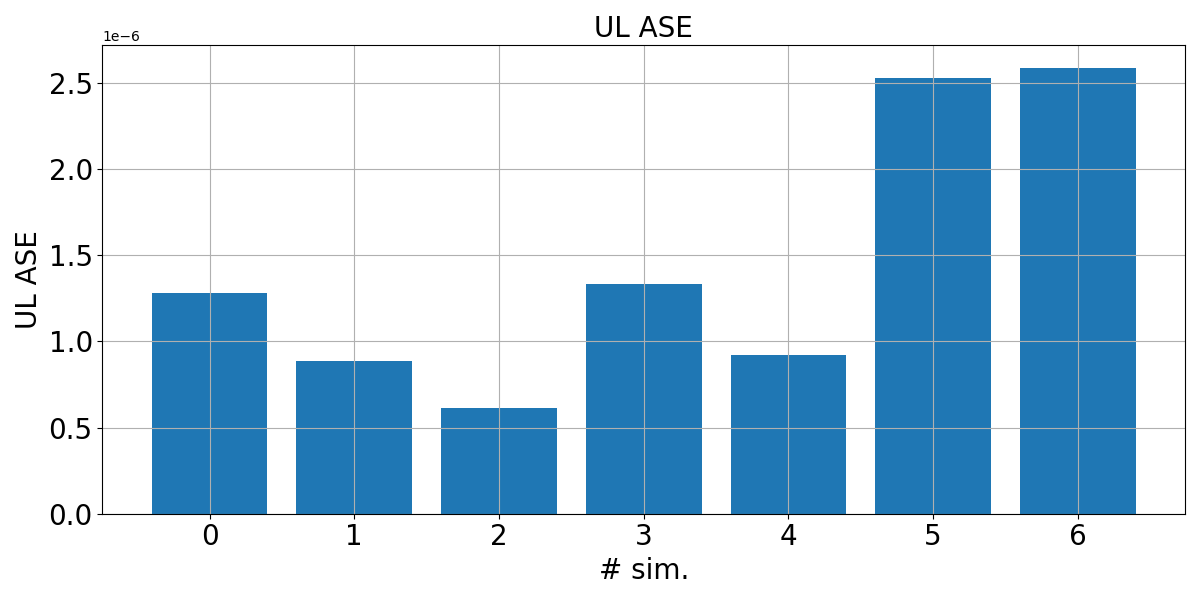
\includegraphics[scale=0.4]{../comparaciones/scheduling_iniciales/ue/ul_ase_multi_sim.png}}
\end{figure}

Se obtienen eficiencias espectrales muy distintas.
En la figura 4.2 se puede ver que las métricas que priorizan la tasa binaria (MT, PF) consiguen mayor eficiencia espectral.

\subsection{Comparación de métricas en LTE y en 5G}

\subsubsection{Introducción}

El artículo \cite{RefWorks:26} describe varios experimentos,
en ellos se analizan las métricas más relevantes de las muchas descritas en el mismo.
Se analizan de manera cuantitativa usando un emulador de nivel de sistema, \textit{LTE-Sim} \cite{RefWorks:69}.

\textit{LTE-Sim} simula la red móvil de LTE, incluyendo la red de acceso E-UTRAN y el núcleo de red (EPS).
Así, \textit{LTE-Sim} soporta la emulación de varias celdas en la red de acceso,
a la que acceden varios usuarios móviles.
Soporta funcionalidades de QoS, traspaso entre celdas, planificación de paquetes, adaptación de enlace mediante AMC, reporte de estado de canal mediante CQI y reutilización de frecuencias.
Para representar la capa física se usa un modelo analítico, que aproxima la capa física.
\cite{RefWorks:69}

Se ha representado el experimento con \textit{FikoRE}
(véase \textit{Caso de uso (X): packet scheduling (italianos)} en el anexo \textit{Simulaciones (metadatos)}).

\subsubsection{Descripción del experimento 1: \textit{un flujo}}

En la primera experiencia, se hace un análisis de las métricas MT, PF, TTA y PF-PF.
El escenario se compone de 19 celdas y un número variable de usarios que van de 20 a 100 (aproximadamente, de 1 a 20 usuarios por celda).
Los usuarios se mueven en una ruta aleatoria (modelo \textit{random way-point}) en torno a la estación base a una velocidad de 30 km/h.
Se considera un tráfico modelado con una fuente de búfer infinito en el enlace descendente para cada UE.
El resto de características del experimento se indican en la tabla 4.1.

\begin{table}[H]
	\ttabbox[\FBwidth]
	{\caption{Planificación de paquetes - Segundo caso - Características del experimento propuesto}}
	{\begin{tabular}{|P{3.0cm}|P{10cm}|}
		\hline
		\textbf{Parámetro} & \textbf{Valor} \\
		\hline
		Duración de la simulación & 100 s \\
		\hline
		Detalles físicos &
		Frecuencia portadora: 2GHz;
		Ancho de banda para DL: 10 MHz;
		Símbolos por TTI: 14;
		Longitud de subtrama: 1 ms;
		Subportadoras por RB: 12;
		Espaciado de subportadoras: 15 kHz;
		Esquema de reutilización de frecuencia: clústeres de cuatro celdas;
		Potencia de transmisión: 43 dBm uniformemente distribuidos entre subcanales;
		Modelo de propagación: Macrocelda urbana (UMa) \\
		\hline
		Adaptación de enlace &
		Modulación: QPSK, 16QAM y 64QAM con todas las tasas de codificación disponibles;
		Objetivo de BLER: $10^{-1}$ \\
		\hline
		Control de encabezado &
		RTP/UDP/IP con compresión ROCH: 3 bytes;
		MAC y RLC: 5 bytes;
		PDCP: 2 bytes;
		CRC: 3 bytes;
		PHY: 3 símbolos \\
		\hline
		Diseño de celda &
		Radio: 0.5 km \\
		\hline
		CQI &
		Método: Todo el ancho de banda y notificación periódica;
		Período de medición: 1 ms \\
		\hline
		Movimiento del UE &
		Modelo de mobilidad: \textit{Random way-point};
		Velocidad del UE: 30 km/h \\
		\hline
		Modelos de tráfico &
		Tipo de tráfico en tiempo real: H264, VoIP;
		Flujos de mejor esfuerzo: búfer infinito \\
		\hline
		\multicolumn{2}{l}{Fuente: \cite{RefWorks:26}}
	\end{tabular}}
\end{table}

Se ha adaptado el mismo experimento para realizarse con el emulador \textit{FikoRE}:

\begin{itemize}
\item Al no moder representarse varias celdas, se ha reducido el experimento a una celda con la misma densidad de UE por celda, es decir, de un UE a 20 UE (caso \textit{pocos}), en concreto: 1 UE, 2 UE, 3 UE, 4 UE, 5 UE, 10 UE, 15 UE, 20 UE.
Adicionalmente, se han simulado en la misma celda una cantidad de UE que iba de 20 a 100 para poder estudiar el comportamiento con elevadas densidades (caso \textit{muchos}), en concreto: 20 UE, 40 UE, 60 UE, 80 UE, 100 UE.
\item Para representar el tráfico de la fuente de búfer infinito se ha generado un tráfico de 100 Mbps en dirección DL en cada UE (caso \textit{un flujo}).
\item Se ha representado el mismo experimento en una celda rural (RMa), que permitía que los UE se desplazaran a gran velocidad (caso \textit{RMa} o caso \textit{rápido}),
y en una celda urbana (UMa), que solo permitía un desplazamiento a menos de 1 km/h (caso \textit{UMa} o caso \textit{lento}).
\item {
Se han probado las distintas métricas de las que disponía \textit{FikoRE}:
\begin{itemize}
\item Caso \textit{RMa-pocos-un flujo}: BET, EDF, FIFO, LWDF, MT, PF, RR.
\item Caso \textit{RMa-muchos-un flujo}: MT, PF.
\item Caso \textit{UMa-pocos-un flujo}: MT, PF.
\item Caso \textit{UMa-muchos-un flujo}: MT, PF.
\end{itemize}
}
\end{itemize}

\begin{figure}[H]
	{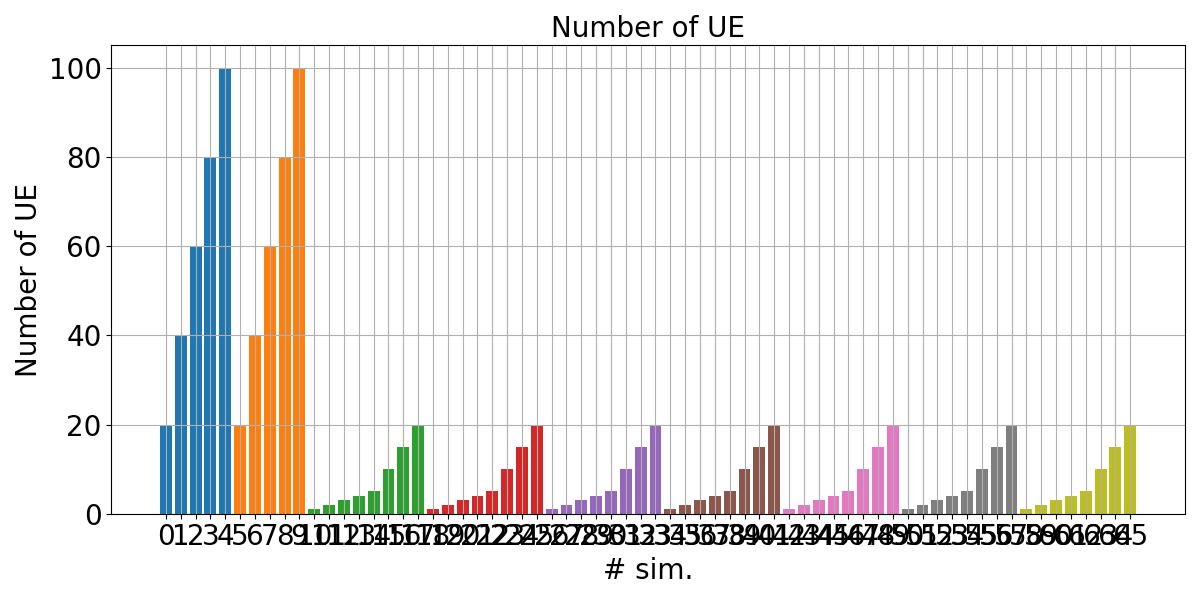
\includegraphics[scale=0.4]{../comparaciones/scheduling_italianos_rma_rapido_1flujo/ue/n_ue_multi_sim.png}}
	\ffigbox[\FBwidth] {
	\caption[Planificación de paquetes - Segundo caso - Nº. de UE (I)]{Número de UE en las distintas simulaciones.

	(Arriba): Caso \textit{RMa-muchos-un flujo} y caso \textit{RMa-pocos-un flujo}.
	Las métricas por orden con el número de simulaciones entre paréntesis: MT (5), PF (5), BET (8), EDF (8), FIFO (8), LWDF (8), MT (8), PF (8), RR (8).

	(Abajo): Caso \textit{UMa-muchos-un flujo} y caso \textit{UMa-pocos-un flujo}.
	Las métricas por orden con el número de simulaciones entre paréntesis: MT (5), PF (5), MT (5), PF (5).}
	}
	{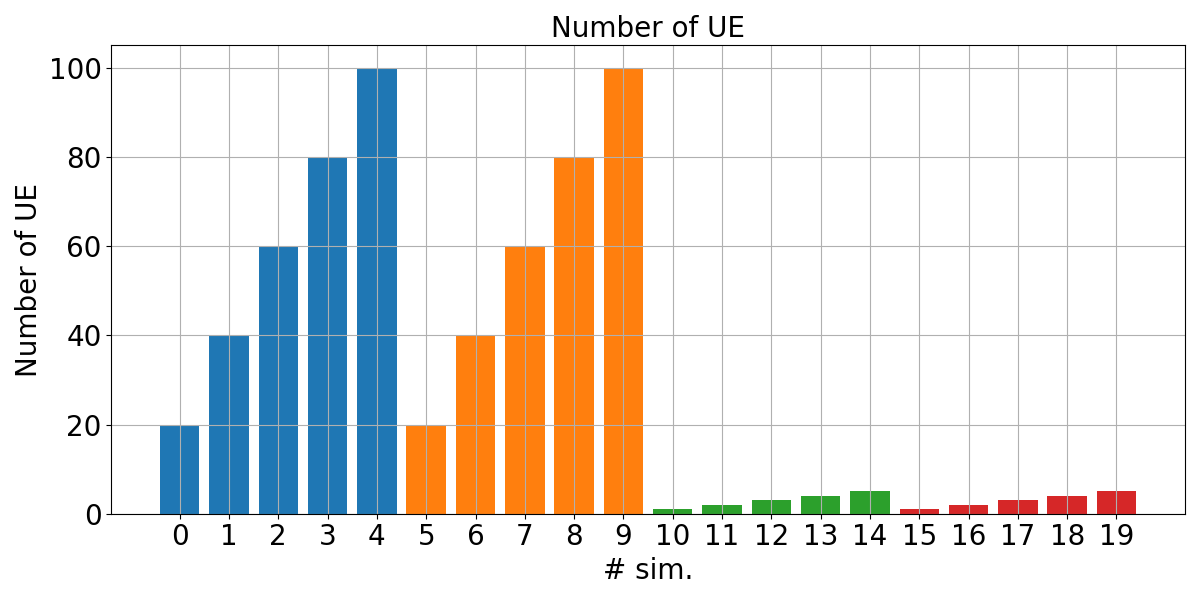
\includegraphics[scale=0.4]{../comparaciones/scheduling_italianos_uma_lento_1flujo/ue/n_ue_multi_sim.png}}
\end{figure}

\subsubsection{Calidad del canal en el experimento 1}

En primer lugar, podemos prever que las prestaciones de la red están limitadas por el ancho de banda, el ruido y la interferencia.
Según la fórmula de Shannon (suponiendo una SINR de 23 dB ó 200):
$$
C = W \log_2 \left( 1 + \frac {S} {N} \right) [b/s] = 10 [MHz] \cdot \log_2 \left( 1 + 200 \right) = 76,511 [Mbps]
$$

En las figuras 4.4 y 4.5,
si atendemos a los valores indicativos del estado del canal de transmisión (SINR, RSRP, CQI),
podemos ver que éstos no cambian entre métricas, solo con el número de UE;
a más UE, peor canal.

{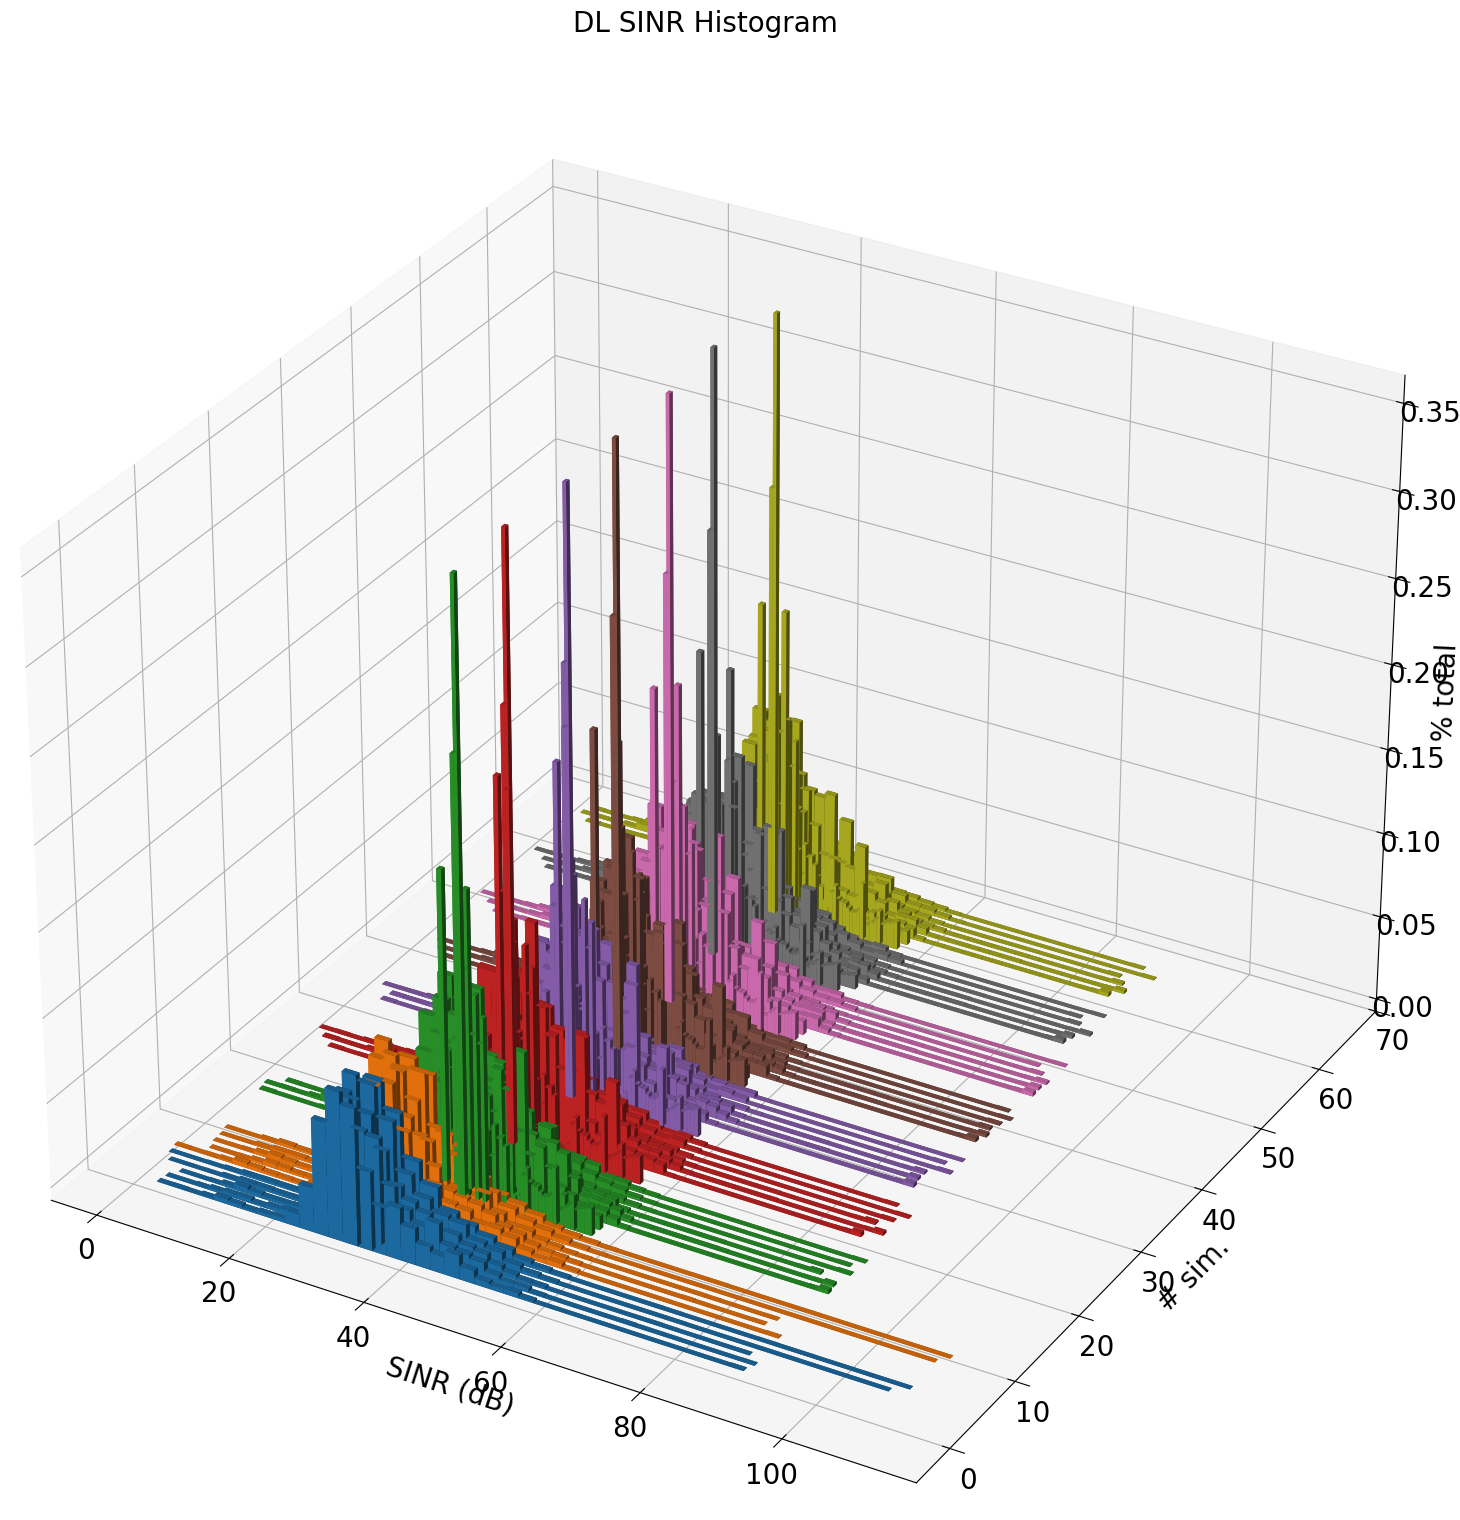
\includegraphics[scale=0.42]{../comparaciones/scheduling_italianos_rma_rapido_1flujo/ue/sinr_dl_3d_hist_all_ue_multi.png_cropped.png}}

{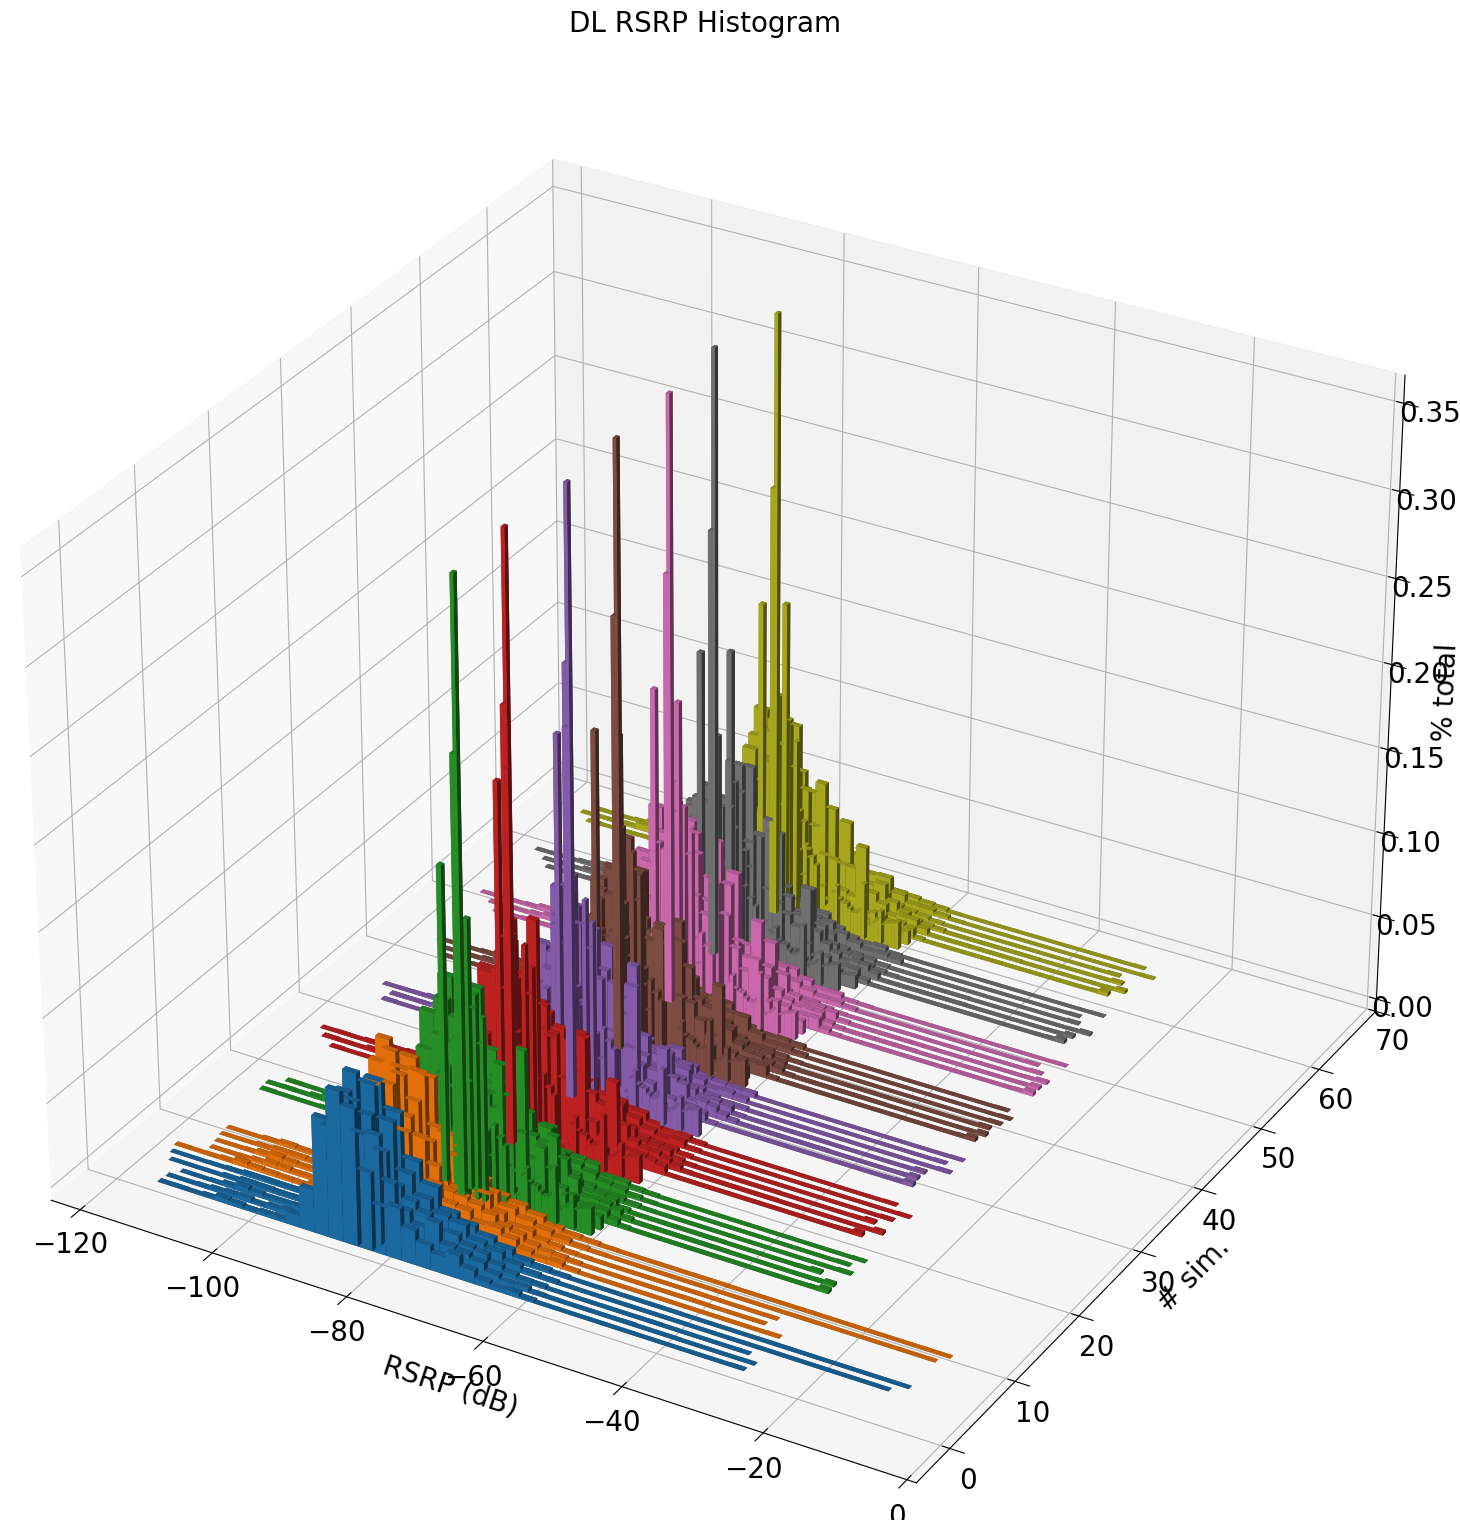
\includegraphics[scale=0.42]{../comparaciones/scheduling_italianos_rma_rapido_1flujo/ue/rsrp_dl_3d_hist_all_ue_multi.png_cropped.png}}

\begin{figure}[H]
	\ffigbox[\FBwidth] {
	\caption[Planificación de paquetes - Segundo caso - Canal (I)]{Distribuciones de los indicadores del estado de canal para la dirección DL en el caso \textit{RMa-muchos-un flujo} y el caso \textit{RMa-pocos-un flujo}.
	Las métricas por orden con el número de simulaciones entre paréntesis: MT (5), PF (5), BET (8), EDF (8), FIFO (8), LWDF (8), MT (8), PF (8), RR (8).

	(Arriba): SINR.

	(Medio): RSRP.

	(Abajo): CQI.}
	}
	{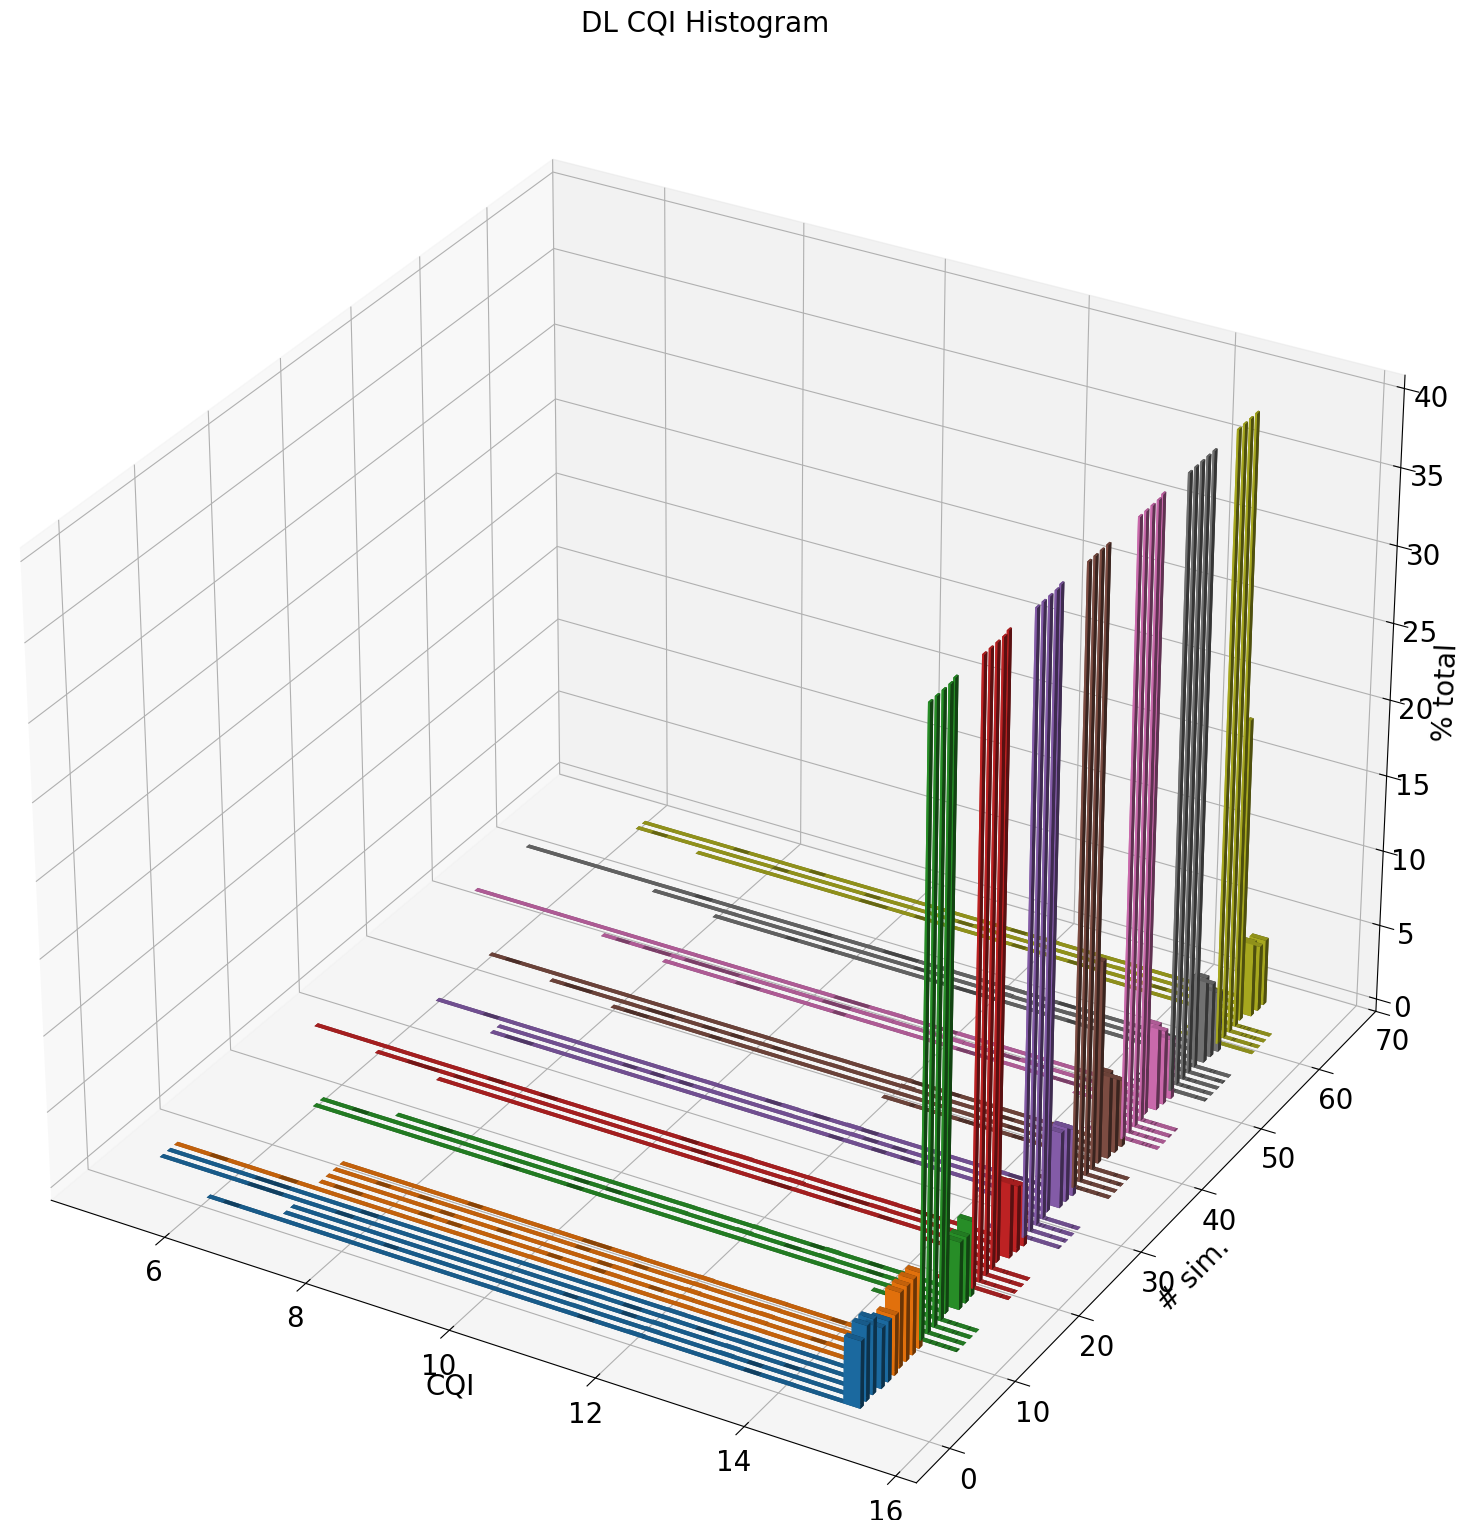
\includegraphics[scale=0.42]{../comparaciones/scheduling_italianos_rma_rapido_1flujo/ue/cqi_dl_3d_hist_all_ue_multi.png_cropped.png}}
\end{figure}

{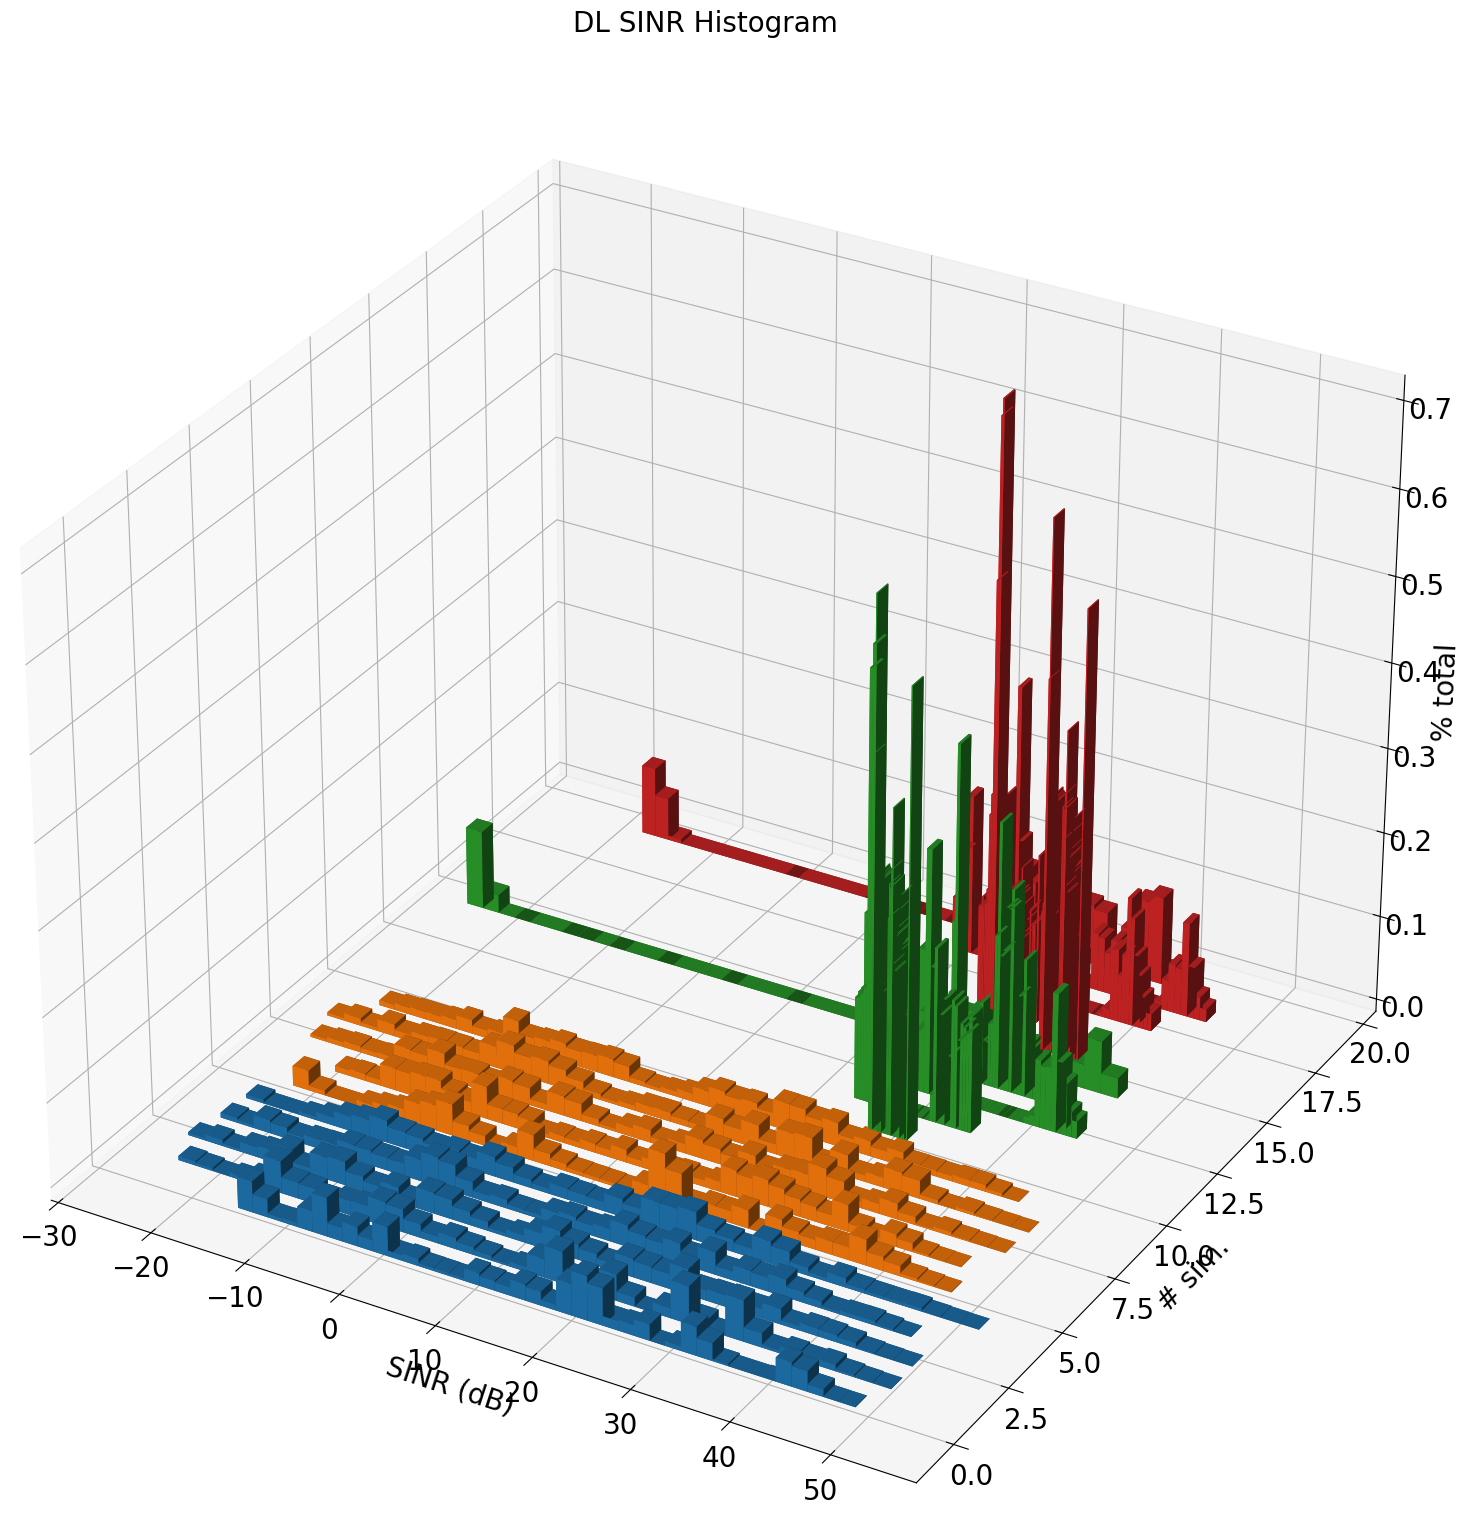
\includegraphics[scale=0.42]{../comparaciones/scheduling_italianos_uma_lento_1flujo/ue/sinr_dl_3d_hist_all_ue_multi.png_cropped.png}}

{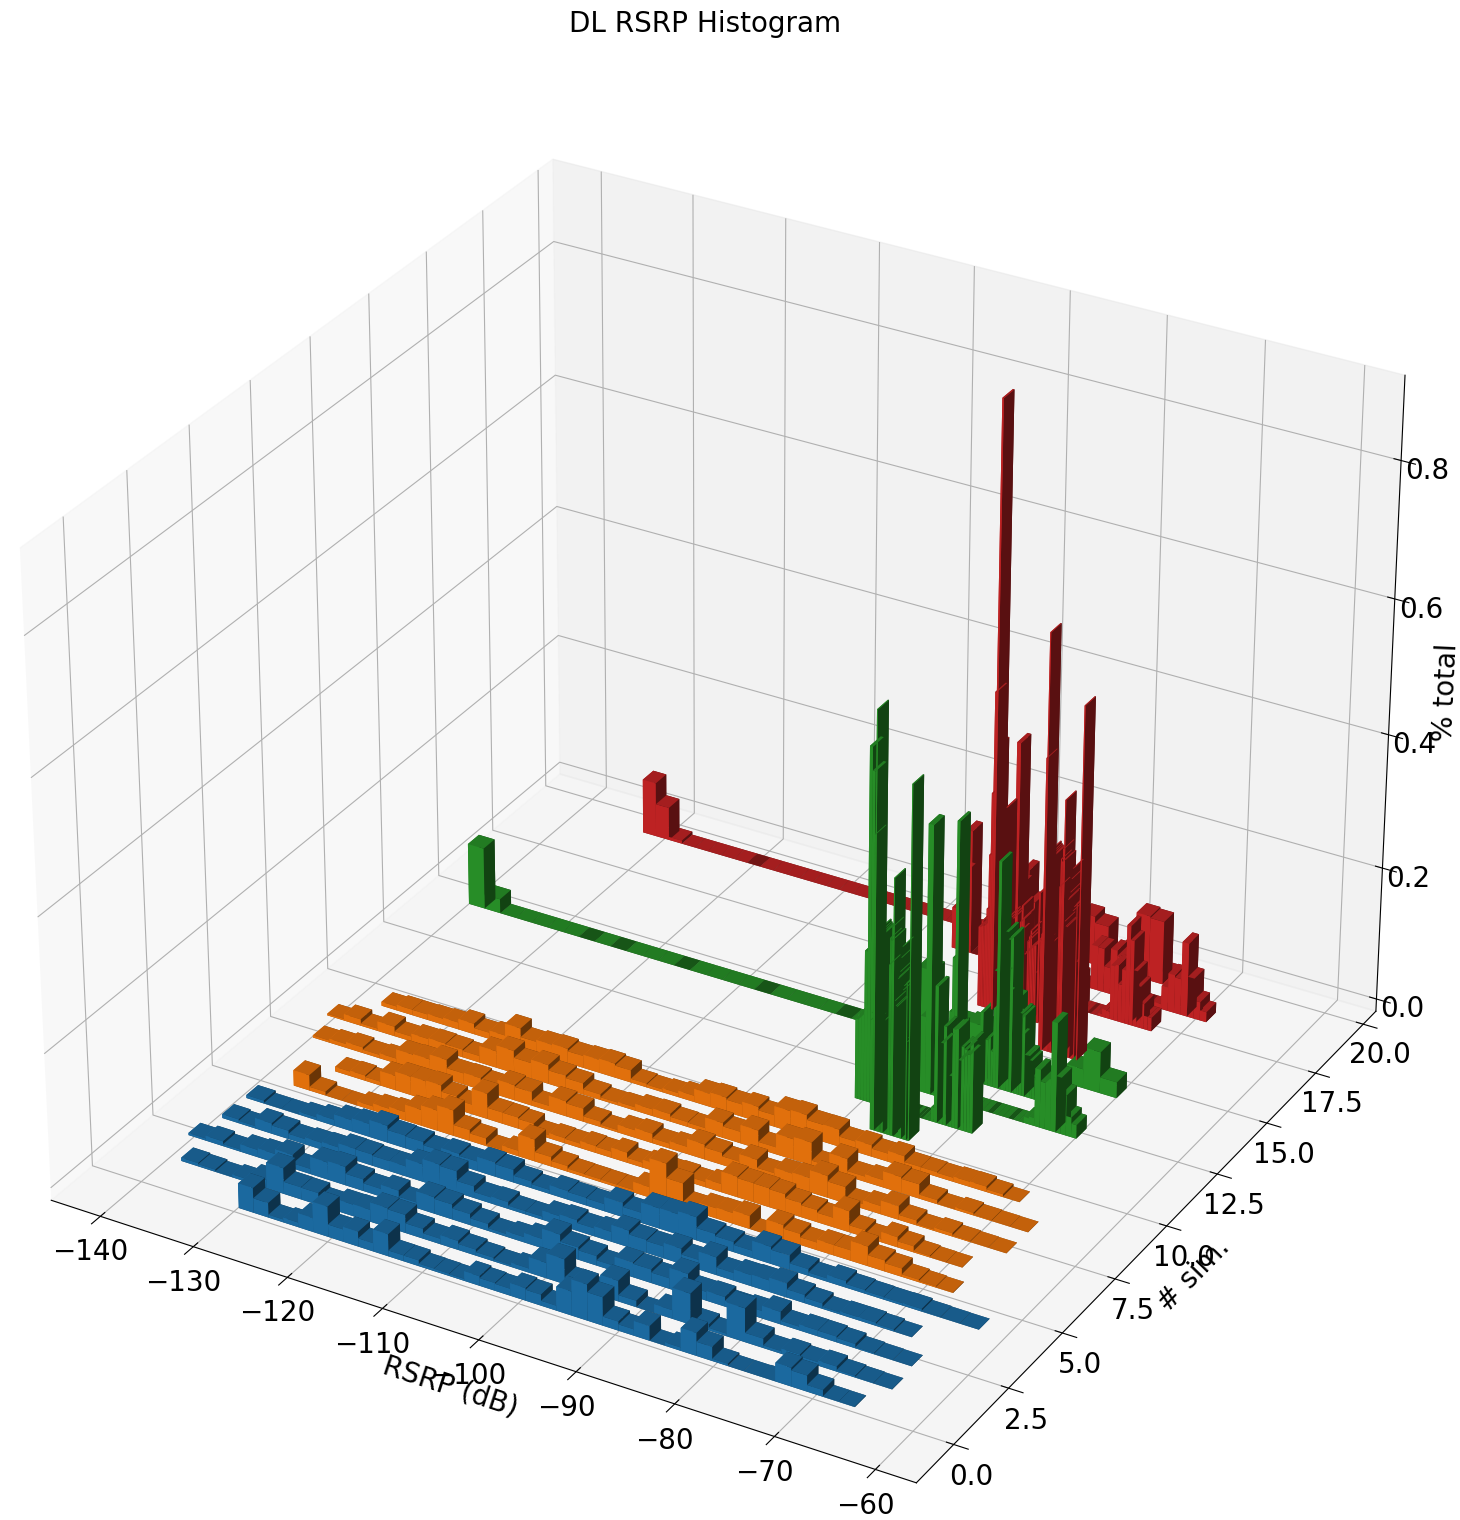
\includegraphics[scale=0.42]{../comparaciones/scheduling_italianos_uma_lento_1flujo/ue/rsrp_dl_3d_hist_all_ue_multi.png_cropped.png}}

\begin{figure}[H]
	\ffigbox[\FBwidth] {
	\caption[Planificación de paquetes - Segundo caso - Canal (II)]{Distribuciones de los indicadores del estado de canal para la dirección DL en el caso \textit{UMa-muchos-un flujo} y el caso \textit{UMa-pocos-un flujo}.
	Las métricas por orden con el número de simulaciones entre paréntesis: MT (5), PF (5), MT (5), PF (5).

	(Arriba): SINR.

	(Medio): RSRP.

	(Abajo): CQI.}
	}
	{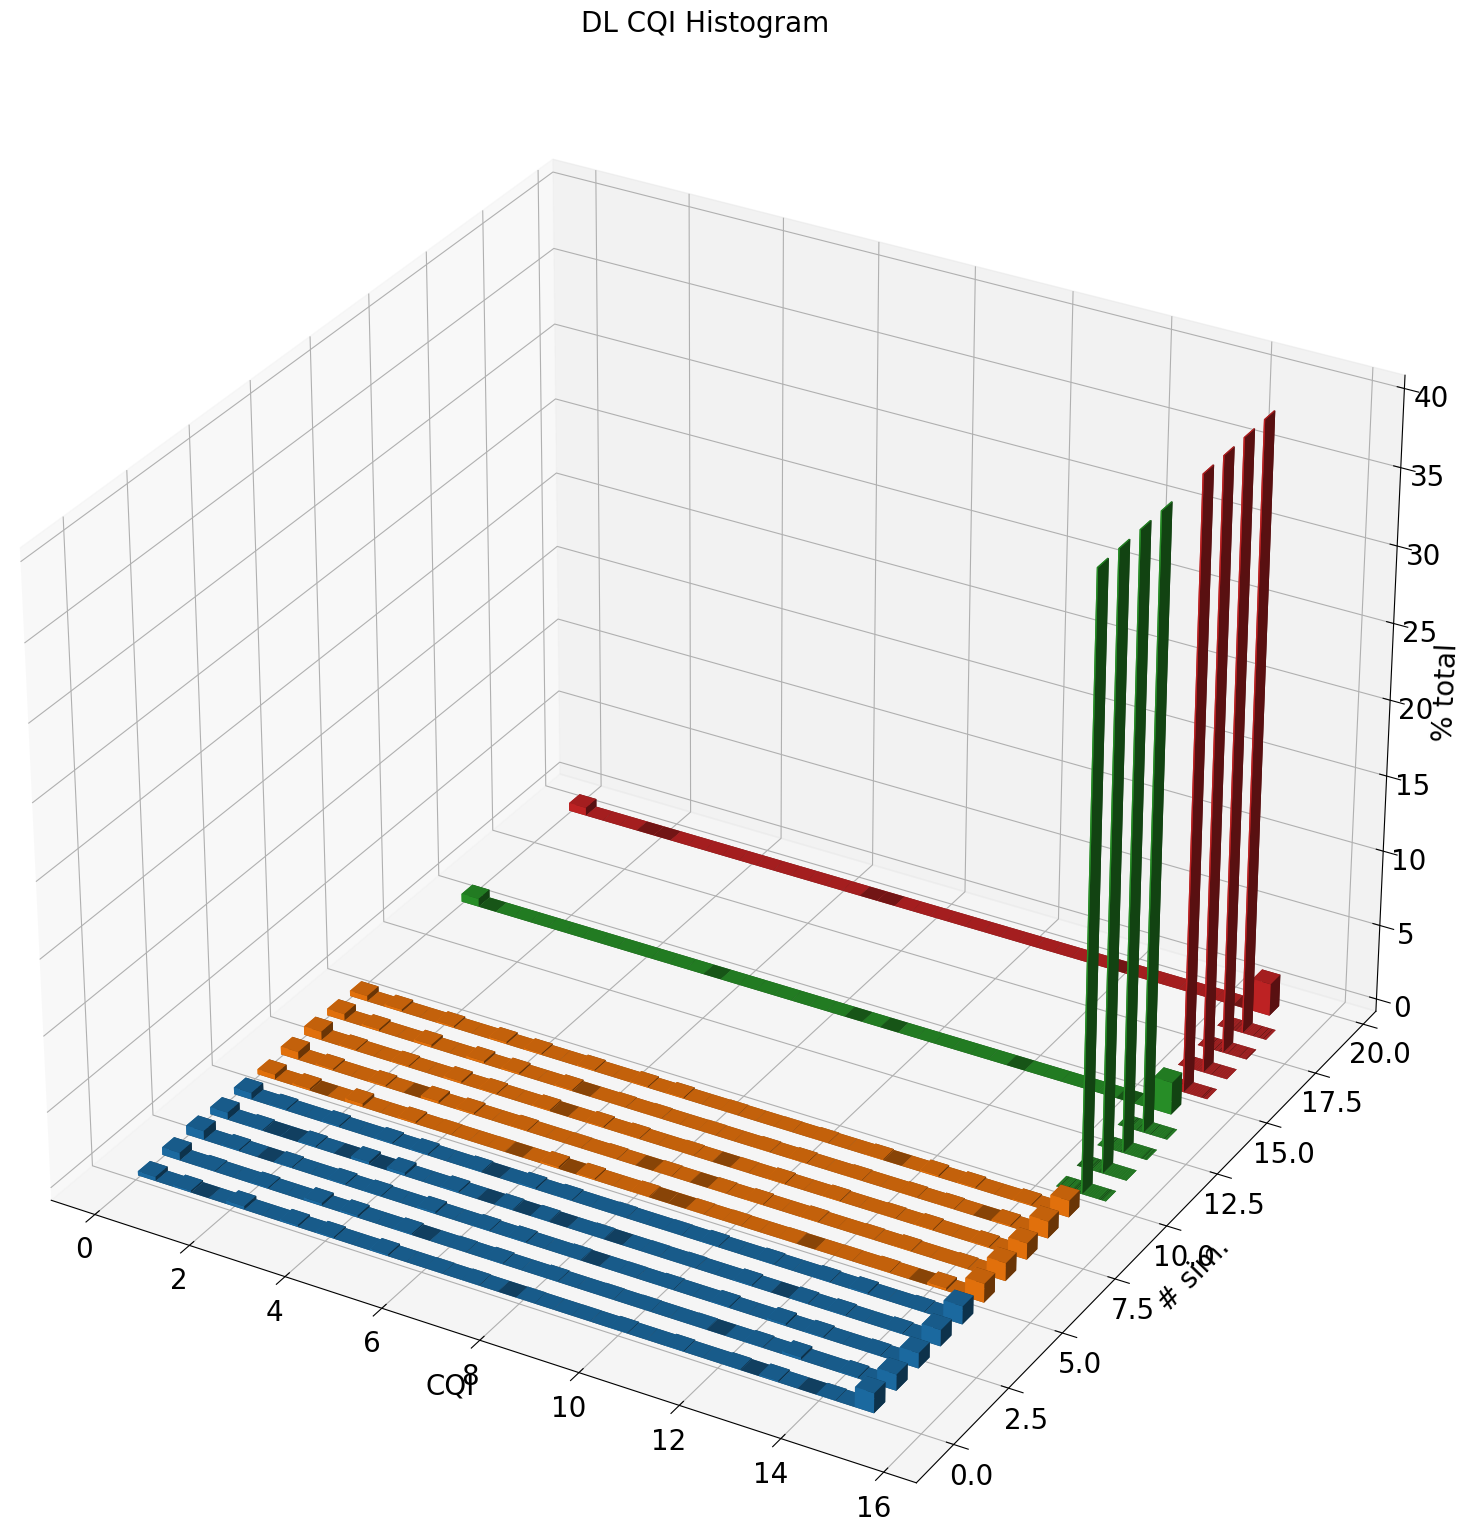
\includegraphics[scale=0.42]{../comparaciones/scheduling_italianos_uma_lento_1flujo/ue/cqi_dl_3d_hist_all_ue_multi.png_cropped.png}}
\end{figure}

Es de esperar, pues el aumento en el número de UE supondrá siempre más interferencia y menos ancho de banda disponible.
Por otro lado, en la celda urbana sí se aprecian distintas distribuciones de RSRP y SINR entre simulaciones;
este comportamiento se puede achacar a la lentitud de estos UE, lo que ocasiona que haya poca variedad de canales y los valores se concentren.

En las figuras 4.6 y 4.6 podemos ver que,
de manera paralela, el índice MCS no cambia entre métricas, sólo entre número de UE en la celda. Además, se concentra en 27 en la RMa y en los valores de 0 y 27 en la UMa:

\begin{figure}[H]
	\ffigbox[\FBwidth] {
	\caption[Planificación de paquetes - Segundo caso - MCS (I)]{Distribución del índice MCS para la dirección DL en el caso \textit{RMa-muchos-un flujo} y el caso \textit{RMa-pocos-un flujo}.
	Las métricas por orden con el número de simulaciones entre paréntesis: MT (5), PF (5), BET (8), EDF (8), FIFO (8), LWDF (8), MT (8), PF (8), RR (8).}
	}
	{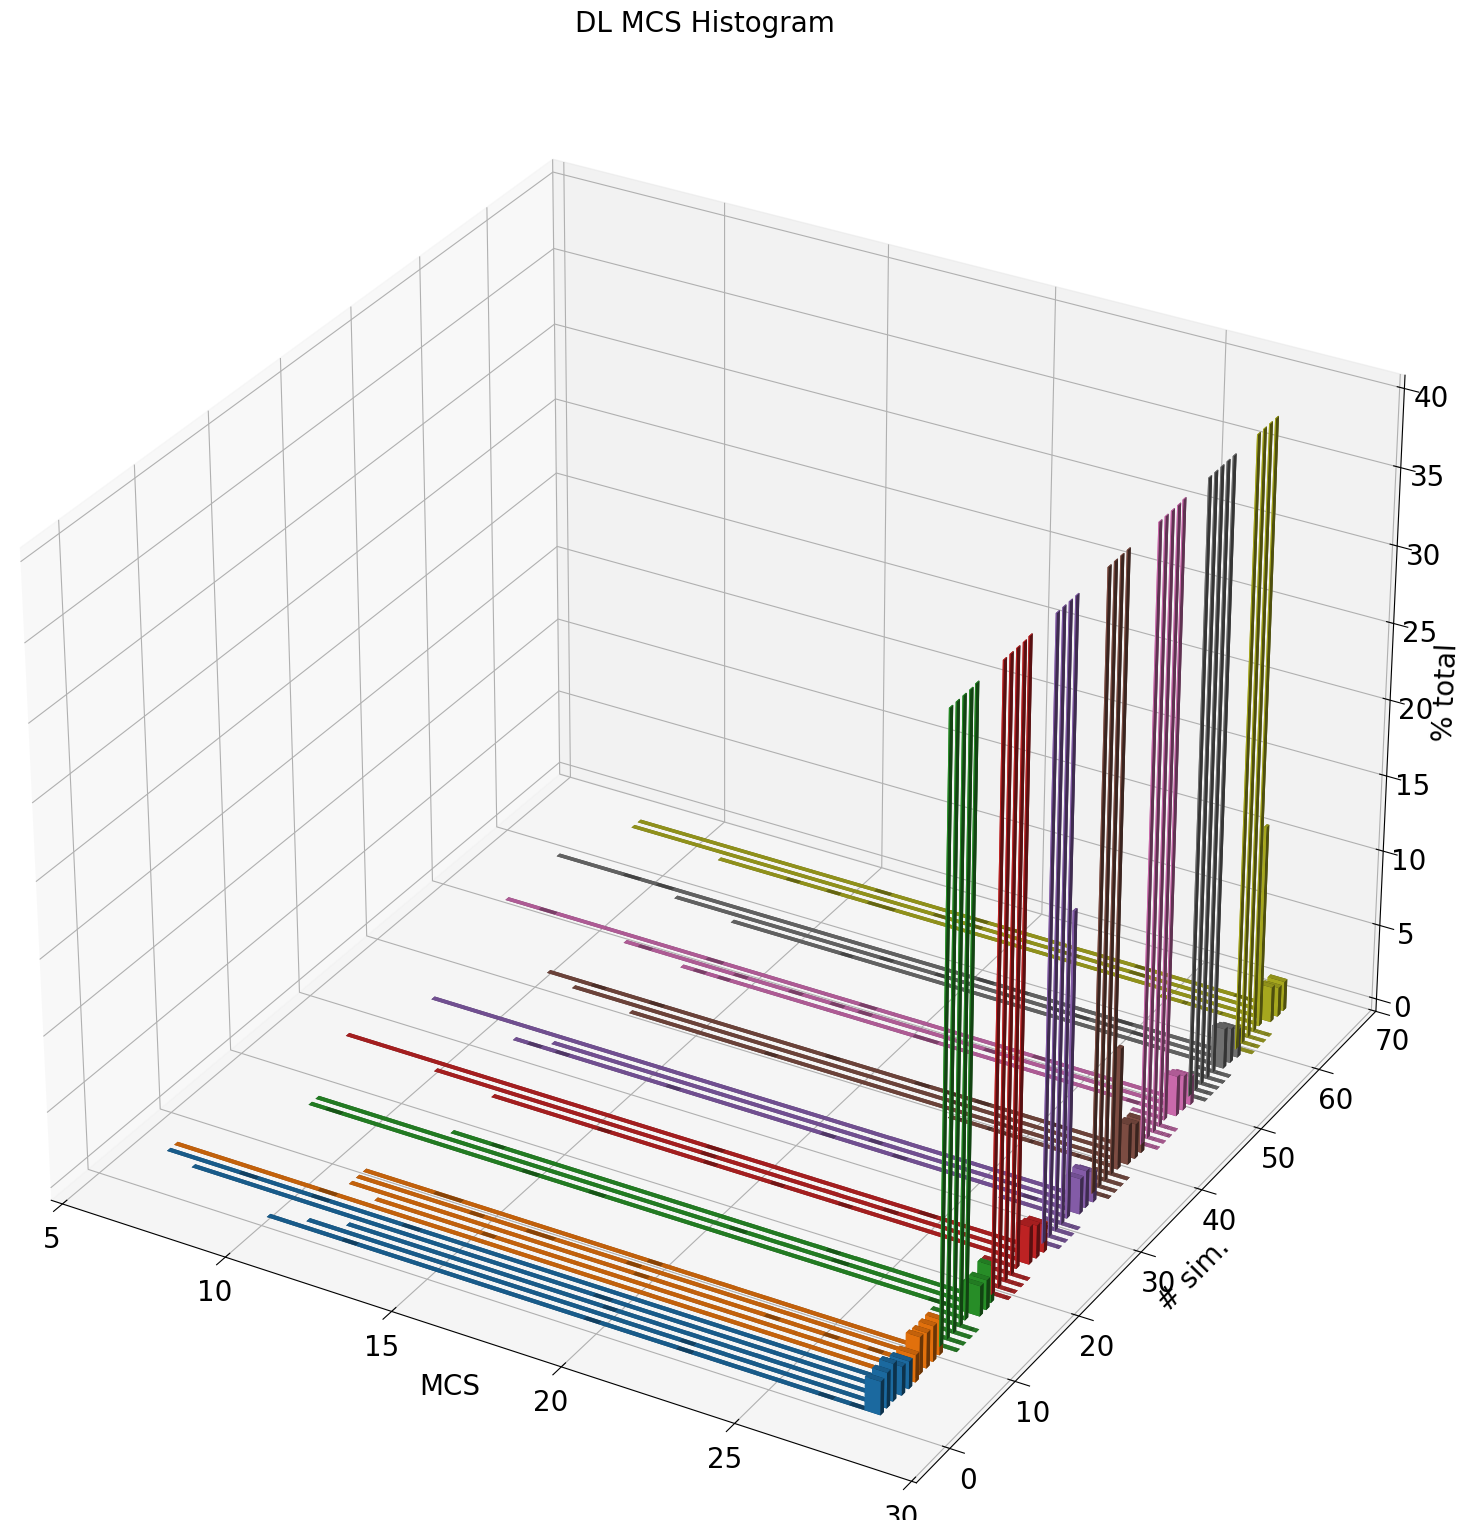
\includegraphics[scale=0.42]{../comparaciones/scheduling_italianos_rma_rapido_1flujo/ue/mcs_dl_3d_hist_all_ue_multi.png_cropped.png}}
\end{figure}

\begin{figure}[H]
	\ffigbox[\FBwidth] {
	\caption[Planificación de paquetes - Segundo caso - MCS (II)]{Distribución del índice MCS para la dirección DL en el caso \textit{UMa-muchos-un flujo} y el caso \textit{UMa-pocos-un flujo}.
	Las métricas por orden con el número de simulaciones entre paréntesis: MT (5), PF (5), MT (5), PF (5).}
	}
	{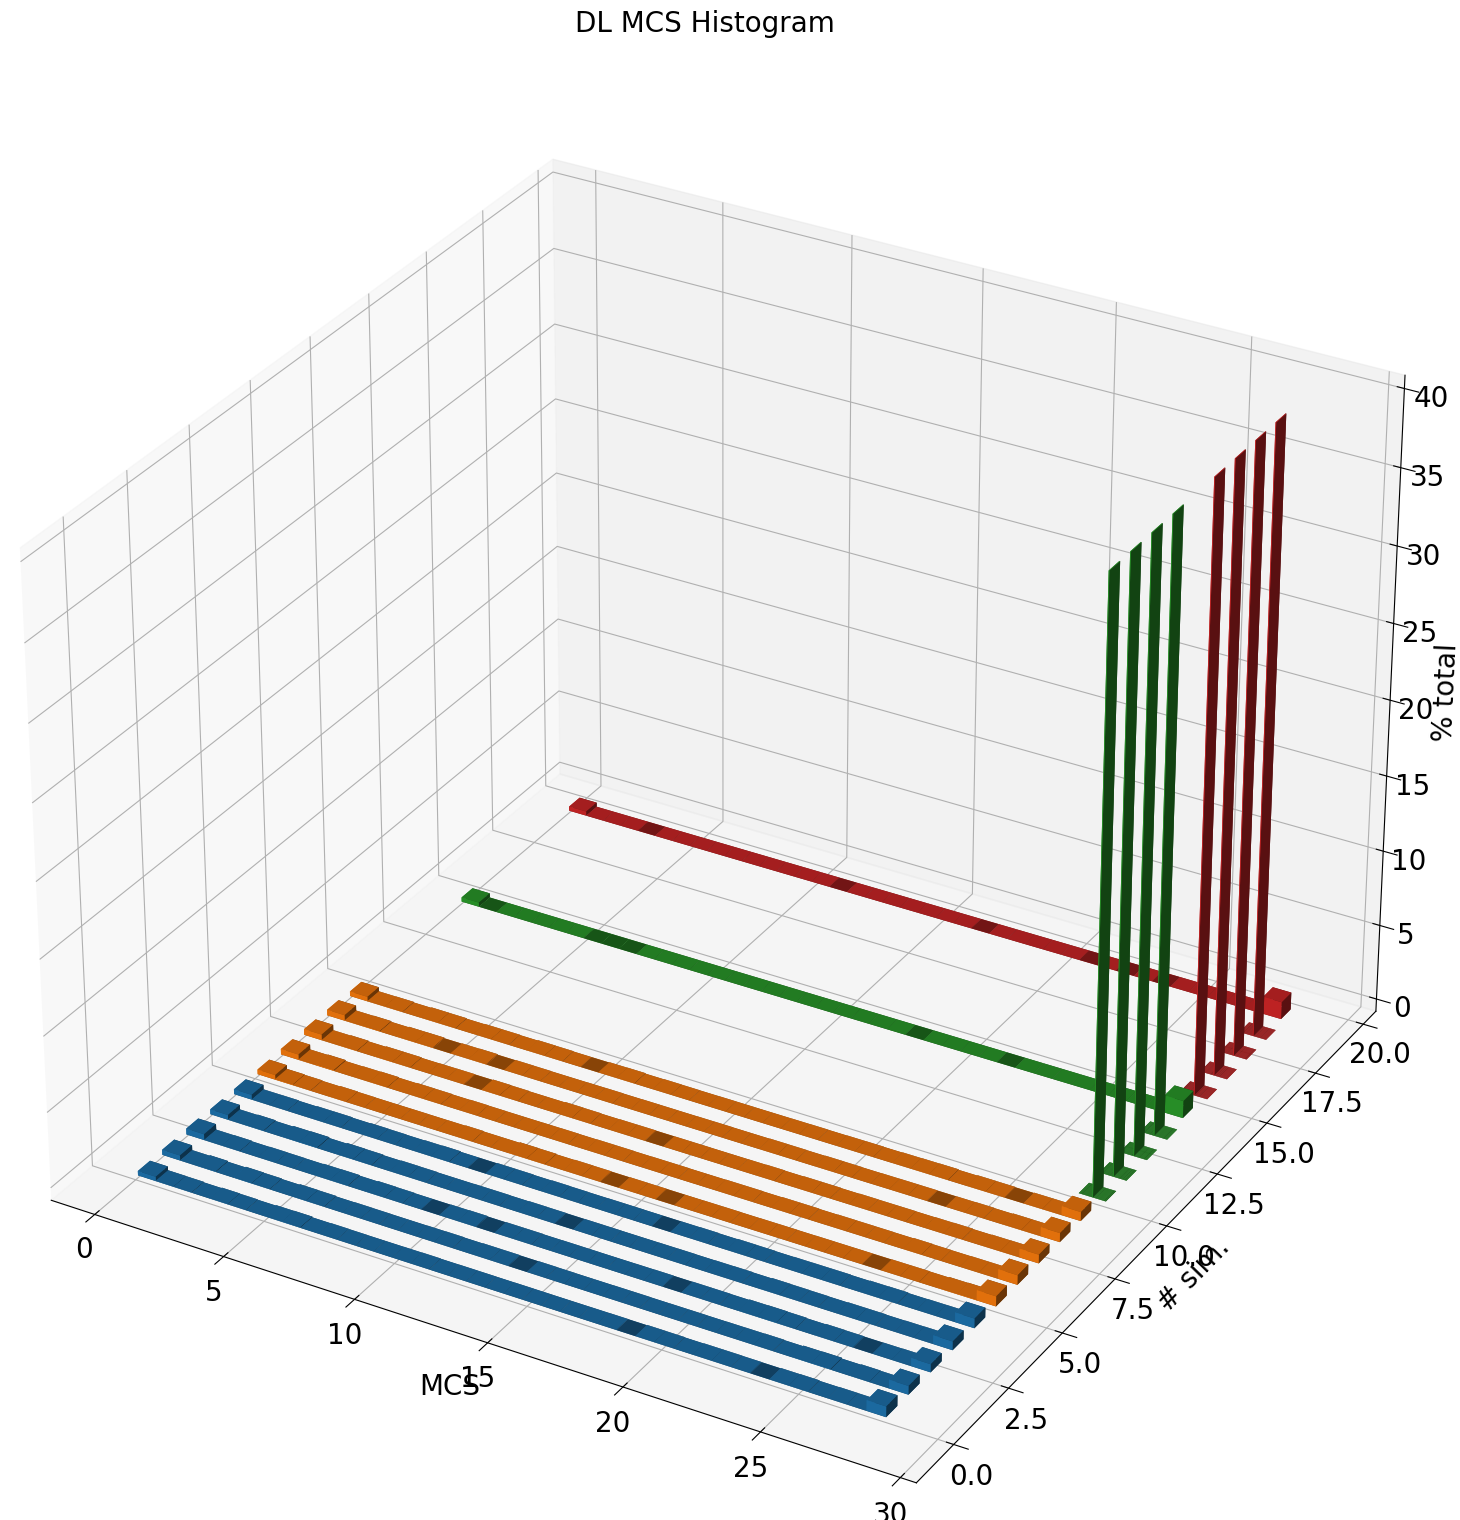
\includegraphics[scale=0.42]{../comparaciones/scheduling_italianos_uma_lento_1flujo/ue/mcs_dl_3d_hist_all_ue_multi.png_cropped.png}}
\end{figure}

Este resultado es, igualmente, esperable, pues los valores SINR, CQI, etc. son los que determinan el valor MCS elegido.
Además, se trata de una celda pequeña, por lo que estos valores son muy parecidos, lo que ocasiona que se concentren en el valor de 27 en la RMa y en los valores de 0 y 27 en la UMa.

\subsubsection{Prestaciones en el experimento 1}

\begin{figure}[H]
	{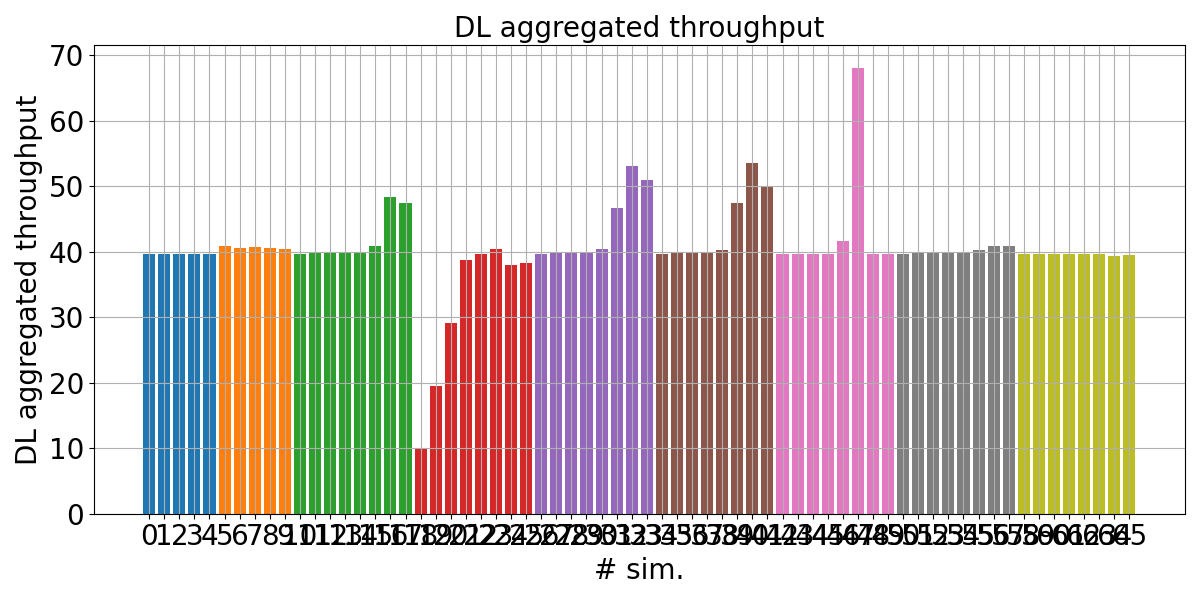
\includegraphics[scale=0.4]{../comparaciones/scheduling_italianos_rma_rapido_1flujo/ue/dl_agg_throughput_multi_sim.png}}
	{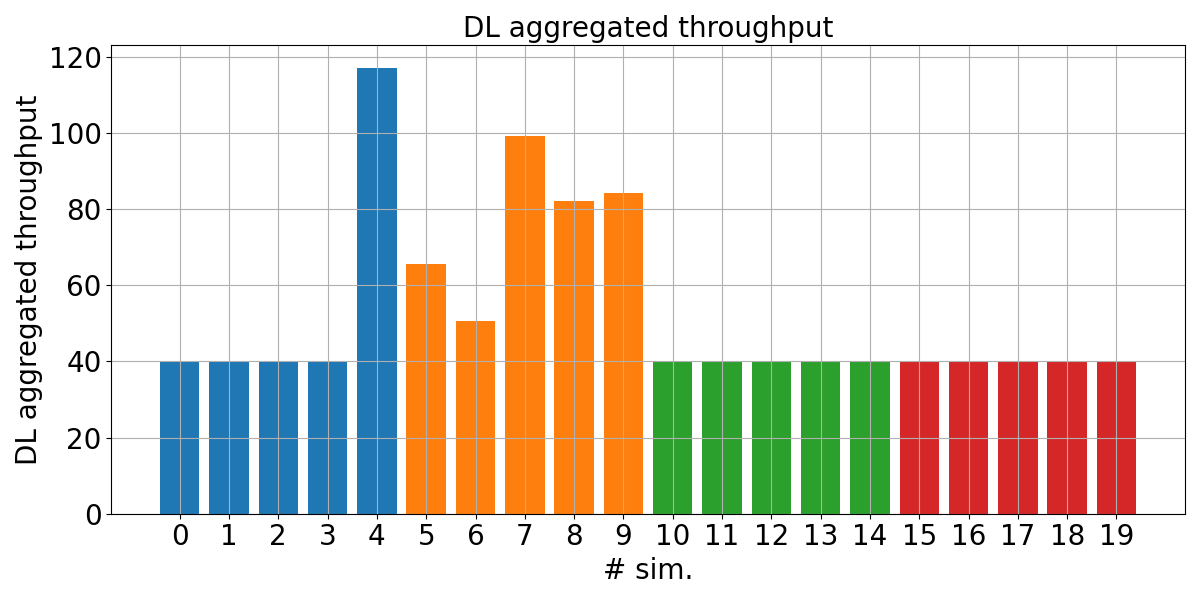
\includegraphics[scale=0.4]{../comparaciones/scheduling_italianos_uma_lento_1flujo/ue/dl_agg_throughput_multi_sim.png}}
	\ffigbox[\FBwidth] {
	\caption[Planificación de paquetes - Segundo caso - Tasa binaria de la celda (I)]{Tasa binaria de la celda.

	(Arriba): Resultados para la dirección DL en el caso \textit{RMa-muchos-un flujo} y el caso \textit{RMa-pocos-un flujo}.
	Las métricas por orden con el número de simulaciones entre paréntesis: MT (5), PF (5), BET (8), EDF (8), FIFO (8), LWDF (8), MT (8), PF (8), RR (8).

	(En medio): Resultados para la dirección DL en el caso \textit{UMa-muchos-un flujo} y el caso \textit{UMa-pocos-un flujo}.
	Las métricas por orden con el número de simulaciones entre paréntesis: MT (5), PF (5), MT (5), PF (5).

	(Abajo): Resultados de \cite{RefWorks:26}.}
	}
	{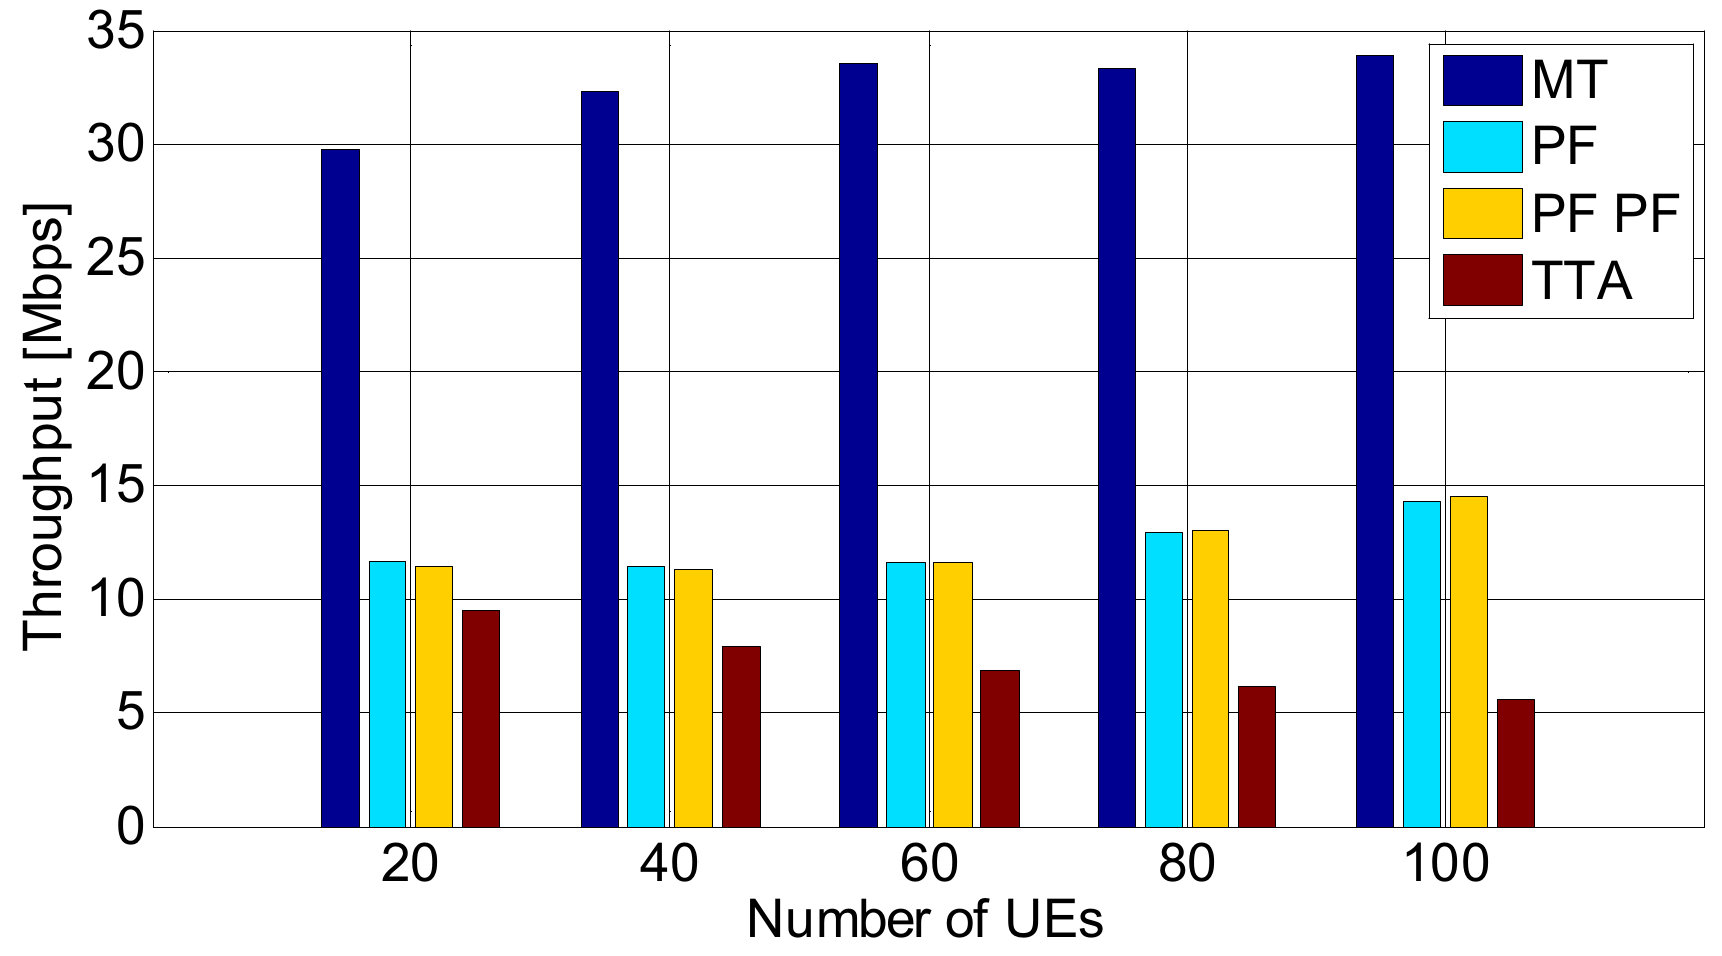
\includegraphics[scale=0.2]{imagenes/scheduling_italianos/scheduling_italianos-199.png}}
\end{figure}

Si ahora vemos la tasa binaria (\textit{throughput}) lograda en la celda, en la figura 4.8, vemos diferentes comportamientos.
En general, la tasa mejora con el número de UE, lo cual, es previsible debido a la \textit{ganancia multiusuario},
que es ocasionada por la mayor cantidad de oportunidades de transmisión que aparecen al aumentar el número de usuarios en una celda.
\cite{RefWorks:26}
También vemos que la tasa binaria es mucho mayor que las logradas en la red LTE en el experimento similar.
Por otro lado, mientras que en \cite{RefWorks:26} las métricas MT y PF ofrecen prestaciones muy diferentes en cuanto a tasa binaria, en este caso son muy similares;
se trata de una diferencia notable de 5G respecto a LTE, pues al disponer la primera de una interfaz de radio mucho más robusta, con calidades de canal superiores, no se aprecian las prioridades de los distintos planificadores.
Este detalle es relevante: MT es la métrica que mejor maximiza la tasa, a costa de empeorar la justicia, mientras que PF hace un balance de tasa y justicia,
ambas métricas pueden tomarse como referencia en adelante.
Otra peculiaridad es que EDF mejora con el número de UE es muy mala con pocos UE;
el resultado tiene que ver con que está diseñada para prevenir la expiración de un tiempo límite, antepone el paquete con el límite más próximo,
no se concentra en elevar la tasa y solo cuando hay varios UE que puedan tener paquetes cerca del límite de expiración aumenta la tasa.
El resto de métricas no muestran ventajas ni inconvenientes adicionales, pero reflejan la misma situación explicada para MT y PF;
la capacidad de la celda simulada es sobrada para que los planificadores no sean tan determinantes.

Por otro lado, es necesario explicar los desiguales resultados del caso que usaba una celda urbana.
Debido a la baja velocidad del UE, no hay variedad de canal;
las simulaciones en celdas urbanas dejan de ser comparables.
De esta manera, en MT el planificador solo atiende al UE más próximo
mientras que PF atiende a entidades de UE con peores canales, resultando en una tasa total superior a la de MT.
La hipótesis puede constatarse viendo una representación de la trayectoria de los UE, como se ve en la figura 4.9.

\begin{figure}[H]
	\ffigbox[\FBwidth] {
	\caption[Planificación de paquetes - Segundo caso - Trayectoria (I)]{Trayectoria de los UE en el caso de la métrica MT con 20 UE del caso \textit{UMa-muchos-un flujo}.}
	}
	{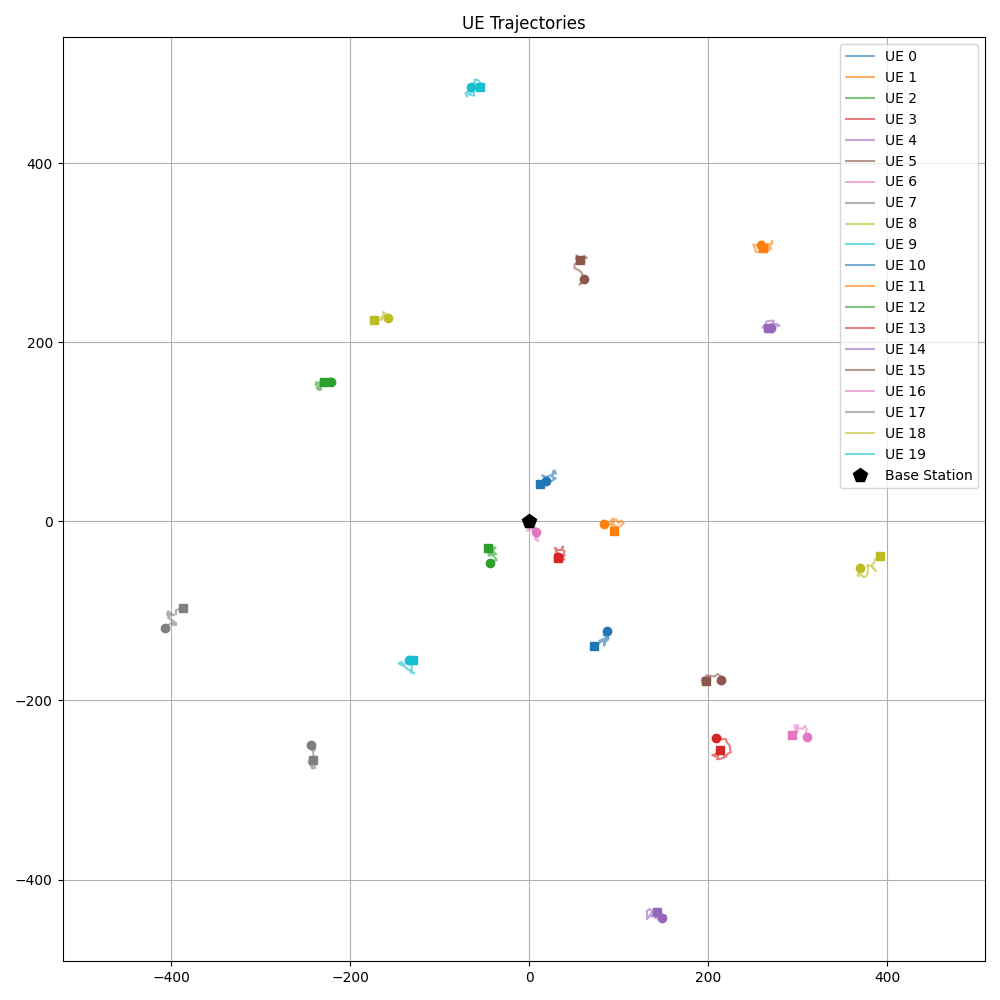
\includegraphics[scale=0.4]{../computos_y_graficas/scheduling_italianos_uma_lento_muchos_1flujo_mt/5_6_21_50_52/ue/trajectory.png}}
\end{figure}

Fijándonos ahora en la tasa de UE promedio, llegaremos a conclusiones similares, con ciertos matices:

\begin{figure}[H]
	{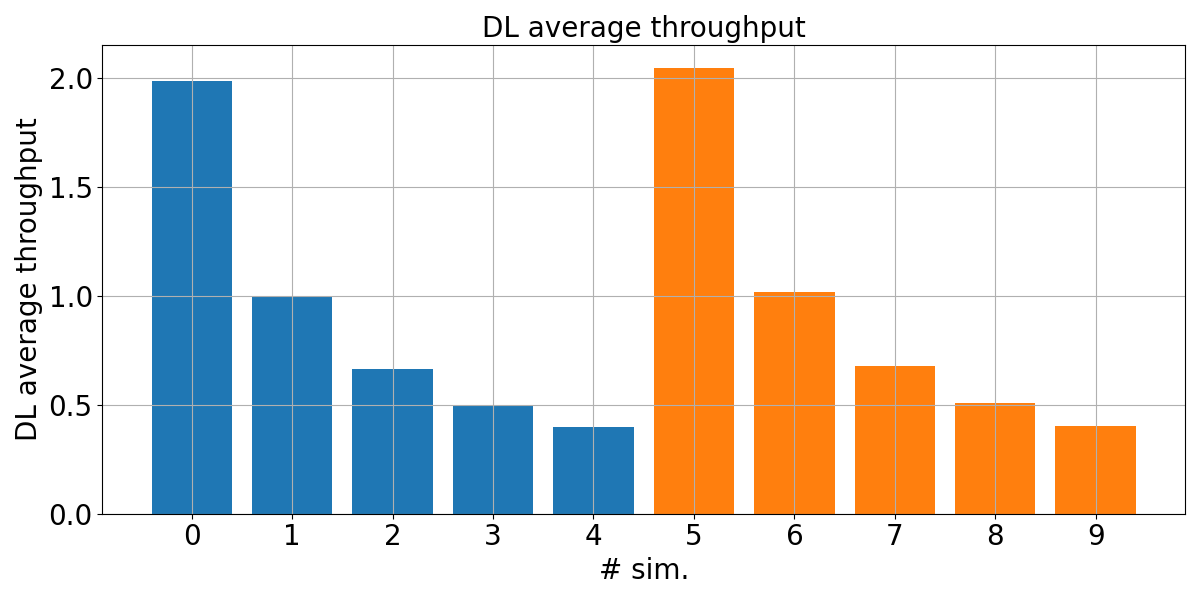
\includegraphics[scale=0.4]{../comparaciones/scheduling_italianos_rma_rapido_muchos_1flujo/ue/dl_ave_throughput_multi_sim.png}}
	{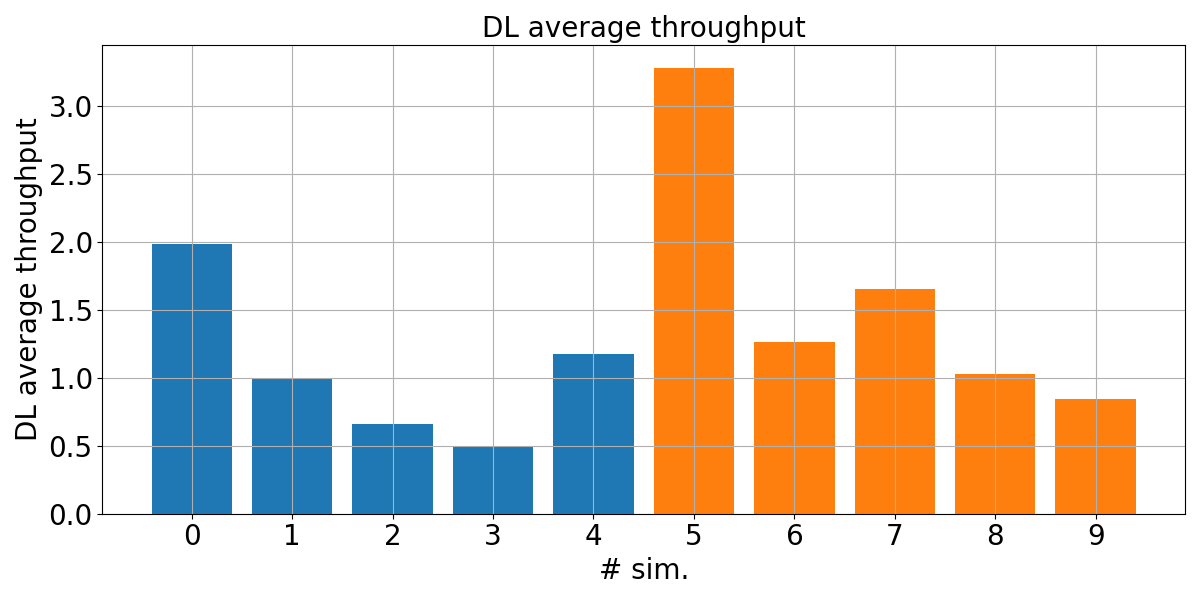
\includegraphics[scale=0.4]{../comparaciones/scheduling_italianos_uma_lento_muchos_1flujo/ue/dl_ave_throughput_multi_sim.png}}
	\ffigbox[\FBwidth] {
	\caption[Planificación de paquetes - Segundo caso - Tasa binaria por UE (I)]{Tasa binaria de un UE en promedio.

	(Arriba): Resultados para la dirección DL en el caso \textit{RMa-muchos-un flujo}.
	Las métricas por orden con el número de simulaciones entre paréntesis: MT (5), PF (5).

	(En medio): Resultados para la dirección DL en el caso \textit{UMa-muchos-un flujo}.
	Las métricas por orden con el número de simulaciones entre paréntesis: MT (5), PF (5).

	(Abajo): Resultados de \cite{RefWorks:26}.}
	}
	{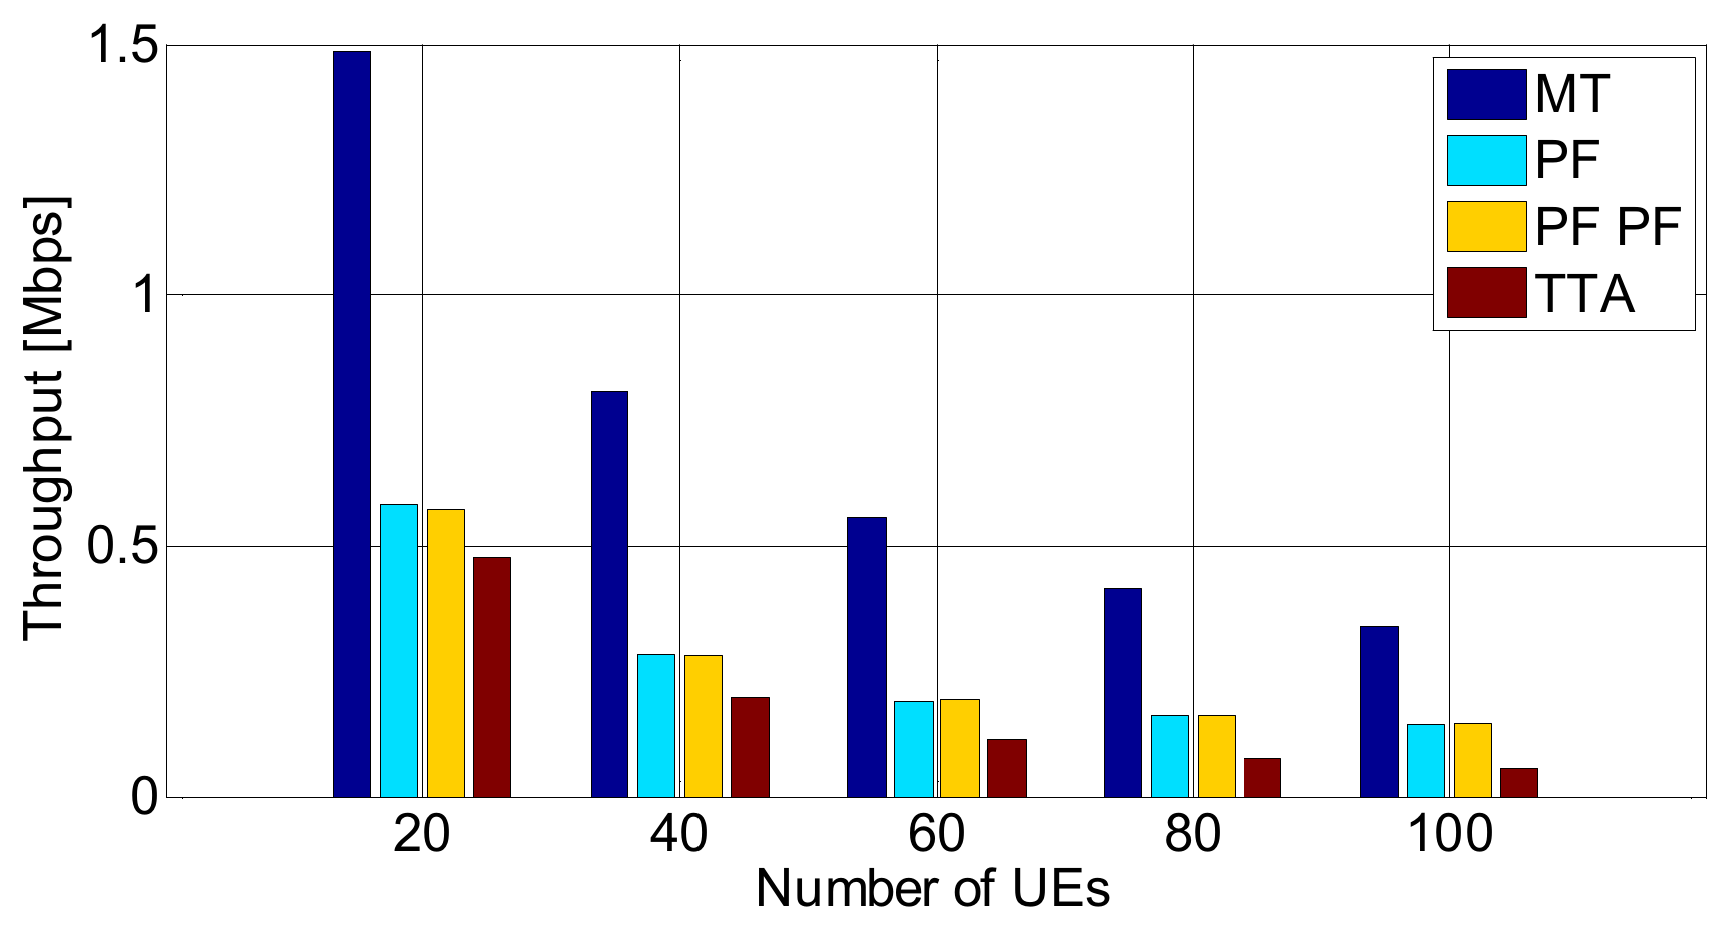
\includegraphics[scale=0.3]{imagenes/scheduling_italianos/scheduling_italianos-200.png}}
\end{figure}

En la figura 4.10 podemos ver que,
en general, la tasa del UE promedio disminuye con el número de UE al tener que compartirse el mismo ancho de banda.
Se puede llegar a las mismas conclusiones antes en lo que respecta a las prestaciones de las métricas MT y PF para la tasa binaria:
debido a la capacidad de 5G no se aprecian las prioridades de los distintos planificadores.

En el caso de la celda urbana, se repite el mismo problema de antes;
al no haber variedad de canal por no desplazarse los UE, la situación inicial es determinante en la calidad de los canales, resultando incluso que con 80 UE haya menor tasa promedio que con 100 UE.

\begin{figure}[H]
	{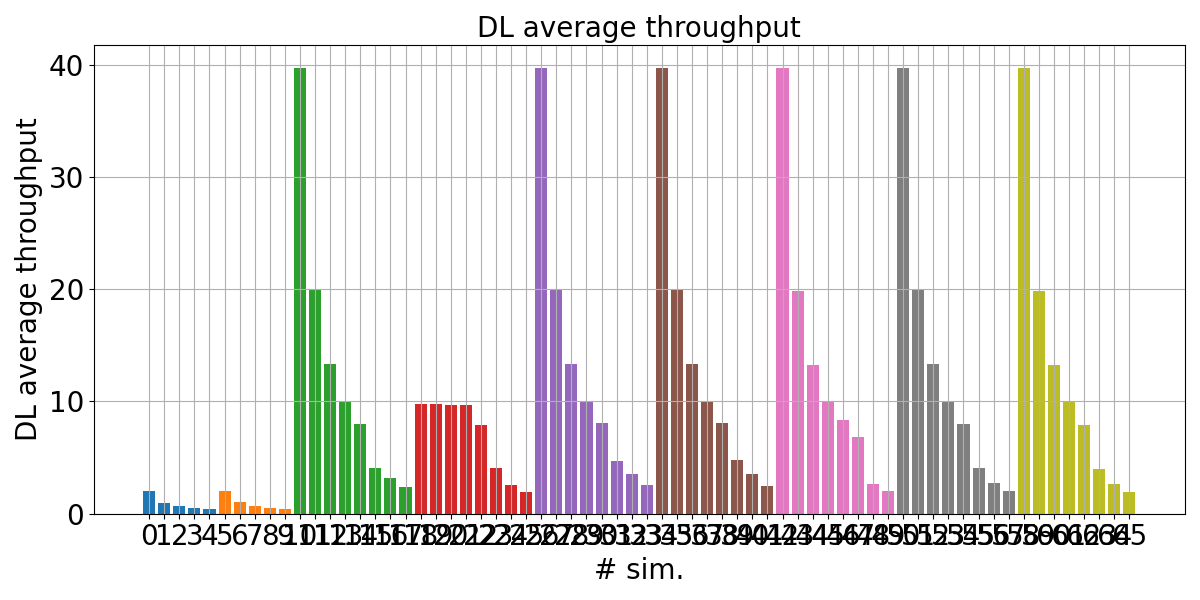
\includegraphics[scale=0.4]{../comparaciones/scheduling_italianos_rma_rapido_1flujo/ue/dl_ave_throughput_multi_sim.png}}
	{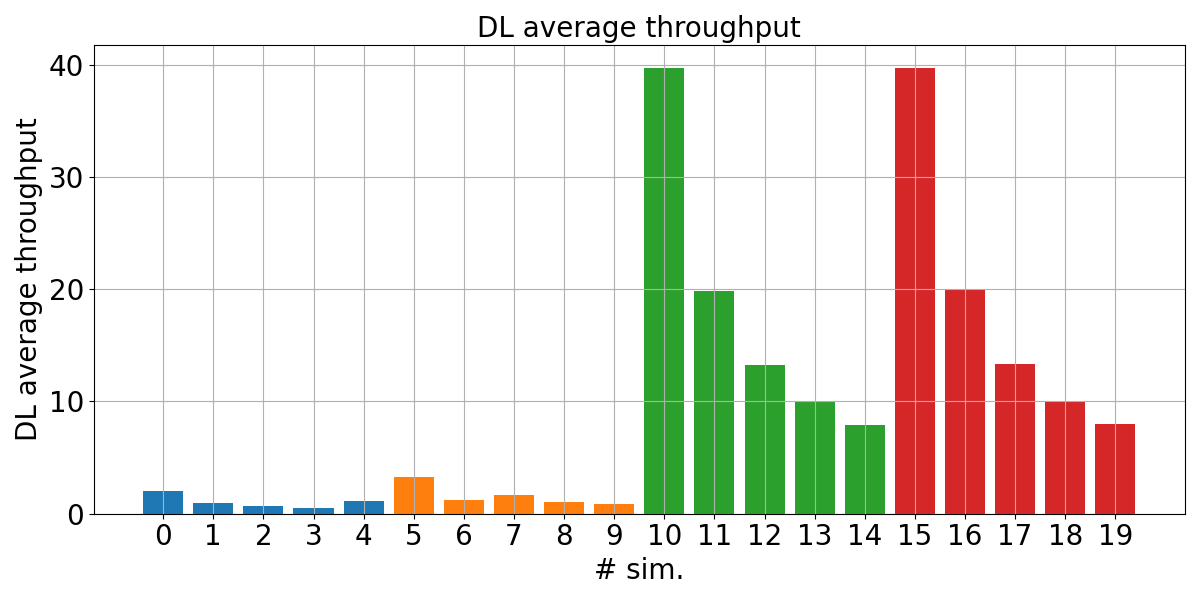
\includegraphics[scale=0.4]{../comparaciones/scheduling_italianos_uma_lento_1flujo/ue/dl_ave_throughput_multi_sim.png}}
	\ffigbox[\FBwidth] {
	\caption[Planificación de paquetes - Segundo caso - Tasa binaria por UE (II)]{Tasa binaria de un UE en promedio.

	(Arriba): Resultados para la dirección DL en el caso \textit{RMa-muchos-un flujo} y el caso \textit{RMa-pocos-un flujo}.
	Las métricas por orden con el número de simulaciones entre paréntesis: MT (5), PF (5), BET (8), EDF (8), FIFO (8), LWDF (8), MT (8), PF (8), RR (8).

	(En medio): Resultados para la dirección DL en el caso \textit{UMa-muchos-un flujo} y el caso \textit{UMa-pocos-un flujo}.
	Las métricas por orden con el número de simulaciones entre paréntesis: MT (5), PF (5), MT (5), PF (5).

	(Abajo): Resultados de \cite{RefWorks:26}.}
	}
	{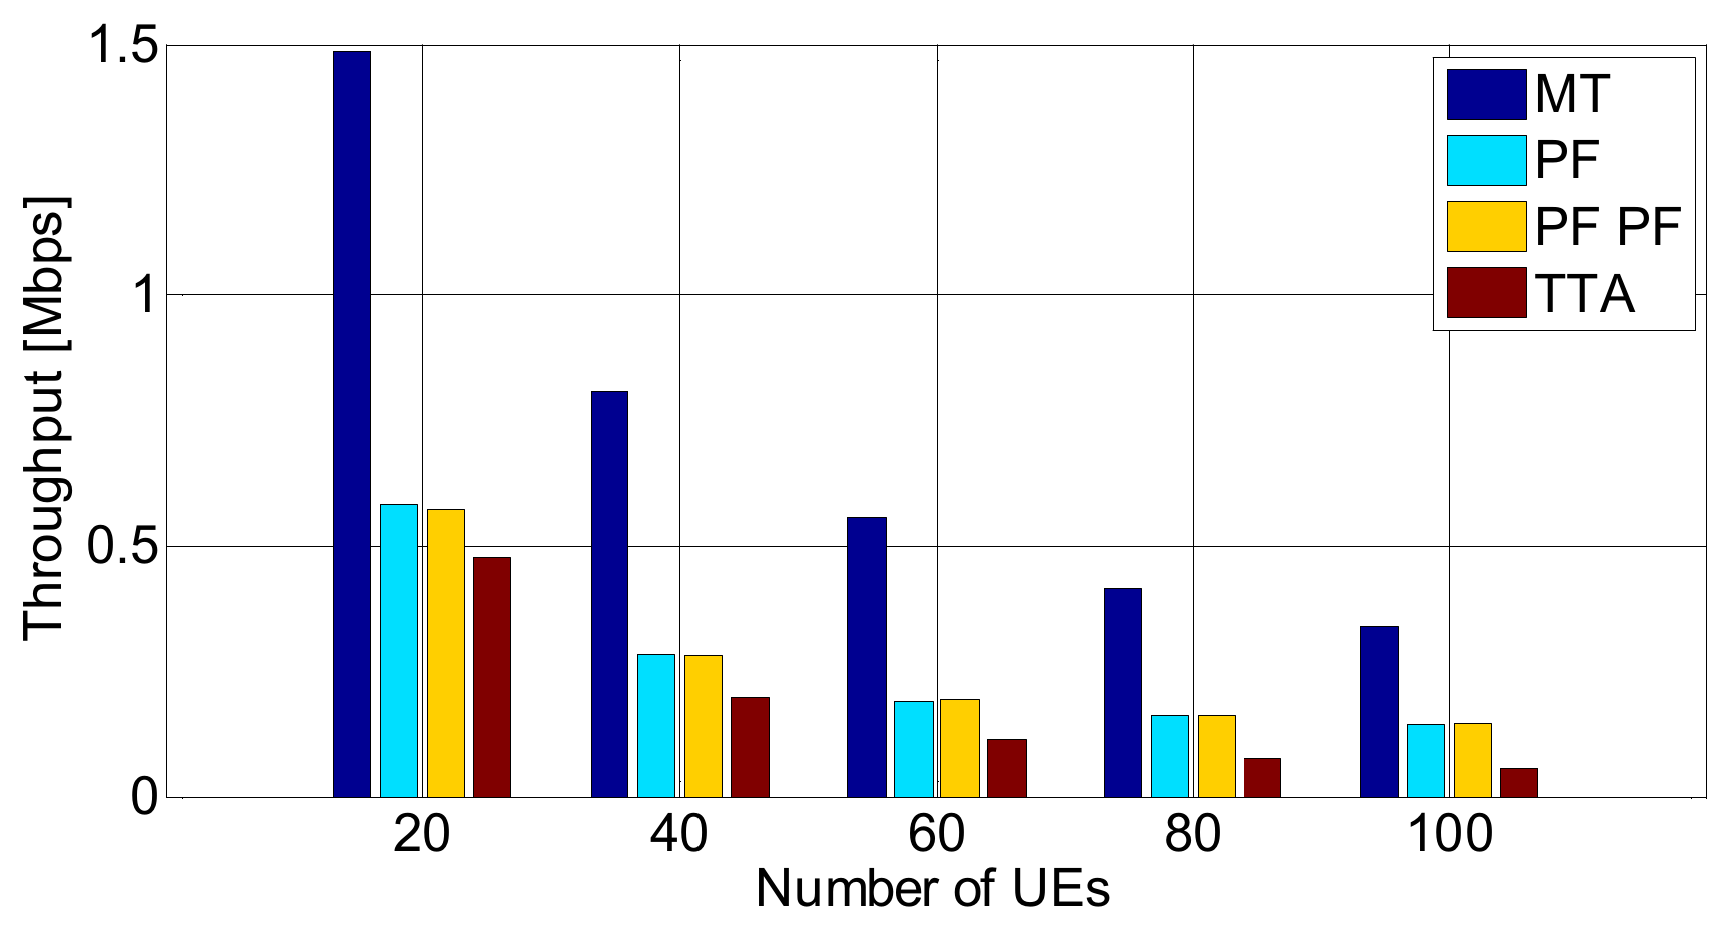
\includegraphics[scale=0.3]{imagenes/scheduling_italianos/scheduling_italianos-200.png}}
\end{figure}

Si ahora incluimos las simulaciones con pocos UE con el resto de métricas, como se ve en la figura 4.11, vemos nuevas diferencias.
Casi todas las métricas ofrecen prestaciones similares por no resultar el planificador determinante.
EDF muestra malas prestaciones con pocos UE, lo que se debe a su diseño centrado en prevenir expiraciones de tiempos límite.

\begin{figure}[H]
	{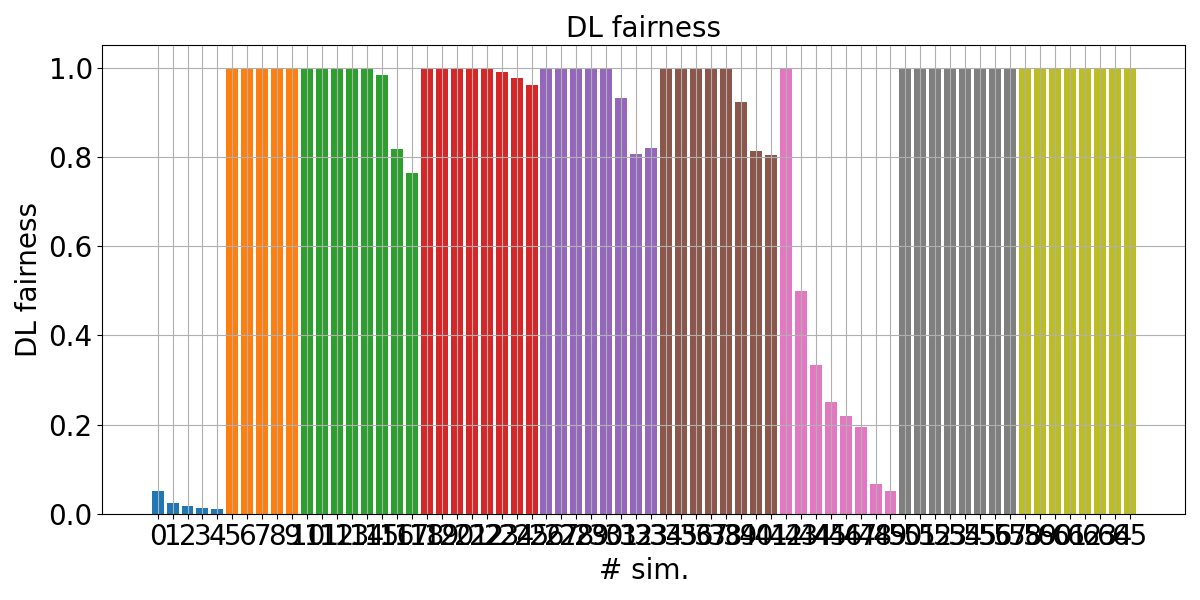
\includegraphics[scale=0.4]{../comparaciones/scheduling_italianos_rma_rapido_1flujo/ue/dl_fairness_multi_sim.png}}
	{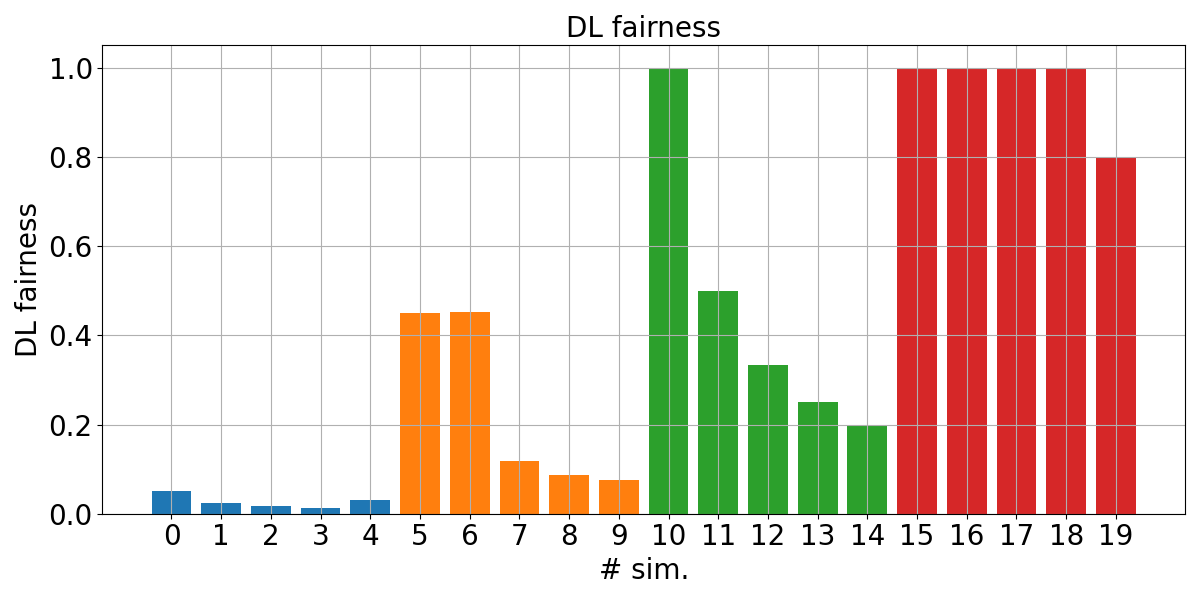
\includegraphics[scale=0.4]{../comparaciones/scheduling_italianos_uma_lento_1flujo/ue/dl_fairness_multi_sim.png}}
	\ffigbox[\FBwidth] {
	\caption[Planificación de paquetes - Segundo caso - Justicia (I)]{Justicia en la celda.

	(Arriba): Resultados para la dirección DL en el caso \textit{RMa-muchos-un flujo} y el caso \textit{RMa-pocos-un flujo}.
	Las métricas por orden con el número de simulaciones entre paréntesis: MT (5), PF (5), BET (8), EDF (8), FIFO (8), LWDF (8), MT (8), PF (8), RR (8).

	(En medio): Resultados para la dirección DL en el caso \textit{UMa-muchos-un flujo} y el caso \textit{UMa-pocos-un flujo}.
	Las métricas por orden con el número de simulaciones entre paréntesis: MT (5), PF (5), MT (5), PF (5).

	(Abajo): Resultados de \cite{RefWorks:26}.}
	}
	{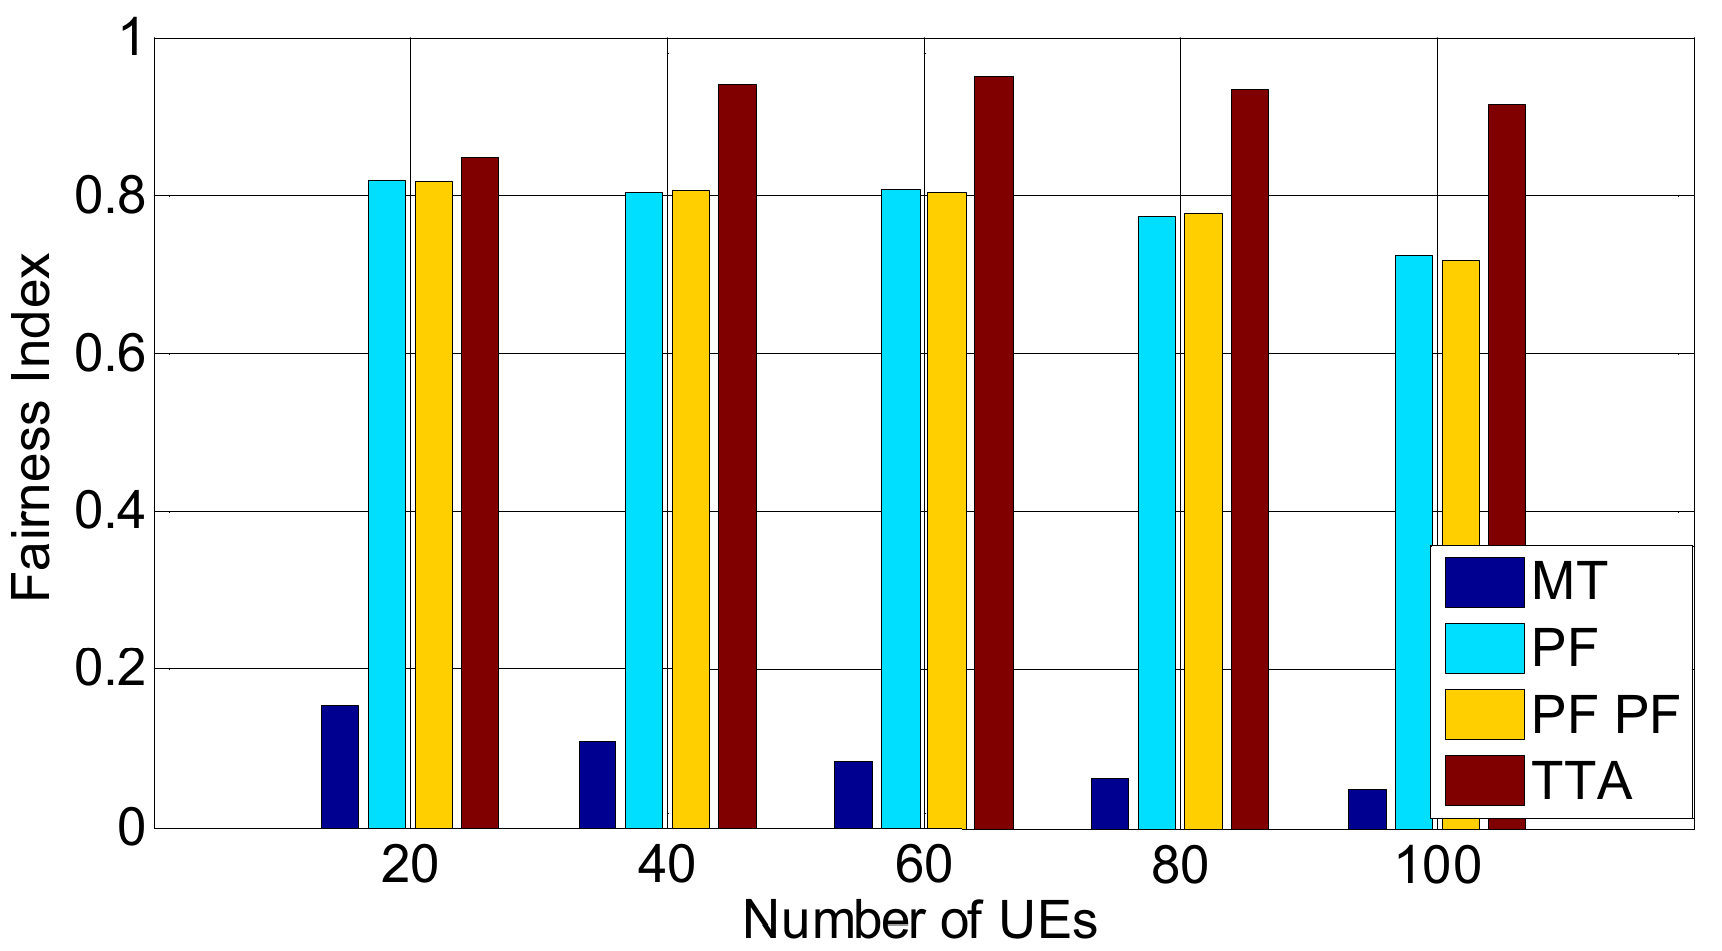
\includegraphics[scale=0.2]{imagenes/scheduling_italianos/scheduling_italianos-201.png}}
\end{figure}

En la figura 4.12 se pueden ver diferentes resultados de justicia lograda.
Cuando hay muchos UE MT da un reparto muy desigual, mientras que PF mantiene cierto nivel de igualdad;
se puede concluir lo mismo descrito en \cite{RefWorks:26}.

En el caso de pocos UE, BET, FIFO y LWDF mantienen el nivel de justicia y empeoran a partir de 15 UE.
Se trata éste de un resultado razonable en cuanto al diseño de estas métricas;
BET es la métrica más justa, a costa de empeorar la tasa;
FIFO es la técnica más simple, es ineficiente e injusta;
LWDF está diseñada para prevenir la expiración de un tiempo límite, maneja probabilidades de pérdida de paquetes.
\cite{RefWorks:26}
Por otro lado EDF, PF y RR mantienen la igualdad por motivos similares sobre su diseño;
EDF está diseñada para prevenir la expiración de un tiempo límite, antepone el paquete con el límite más próximo;
PF hace un balance de tasa y justicia;
la métrica RR se diseña modificando FIFO para añadir justicia.
Por su parte, MT empeora muy rápido al crecer el número de UE porque está diseñada para maximizar la tasa.

\begin{center}{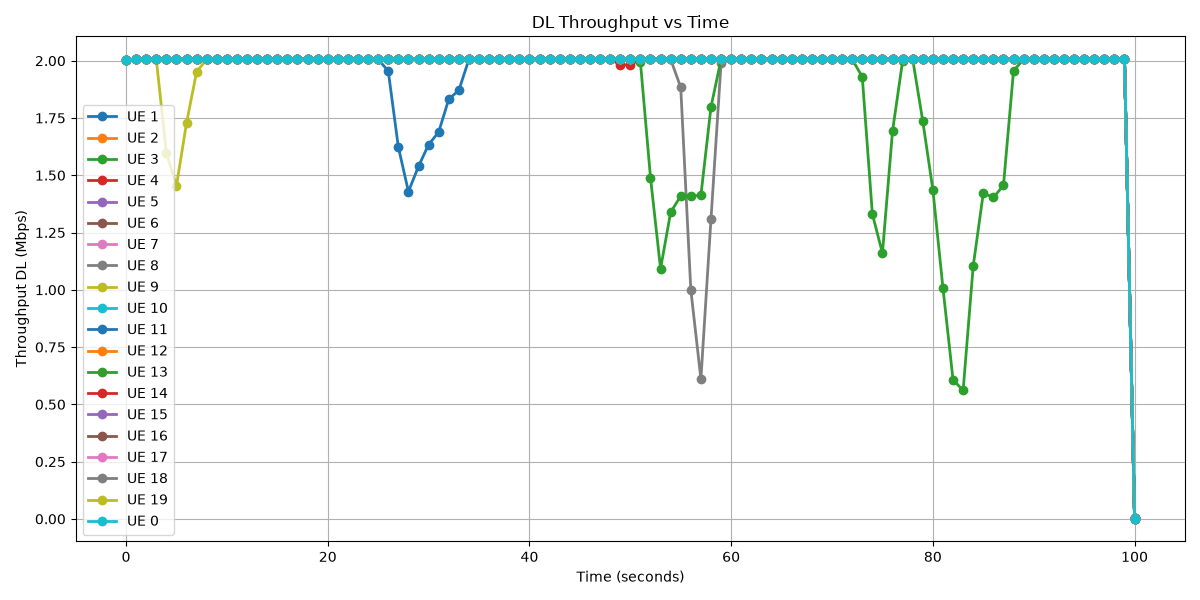
\includegraphics[scale=0.35]{../computos_y_graficas/scheduling_italianos_rma_rapido_pocos_1flujo_rr/5_7_17_28_55/mac/dl_throughput.png}}\end{center}

\begin{center}{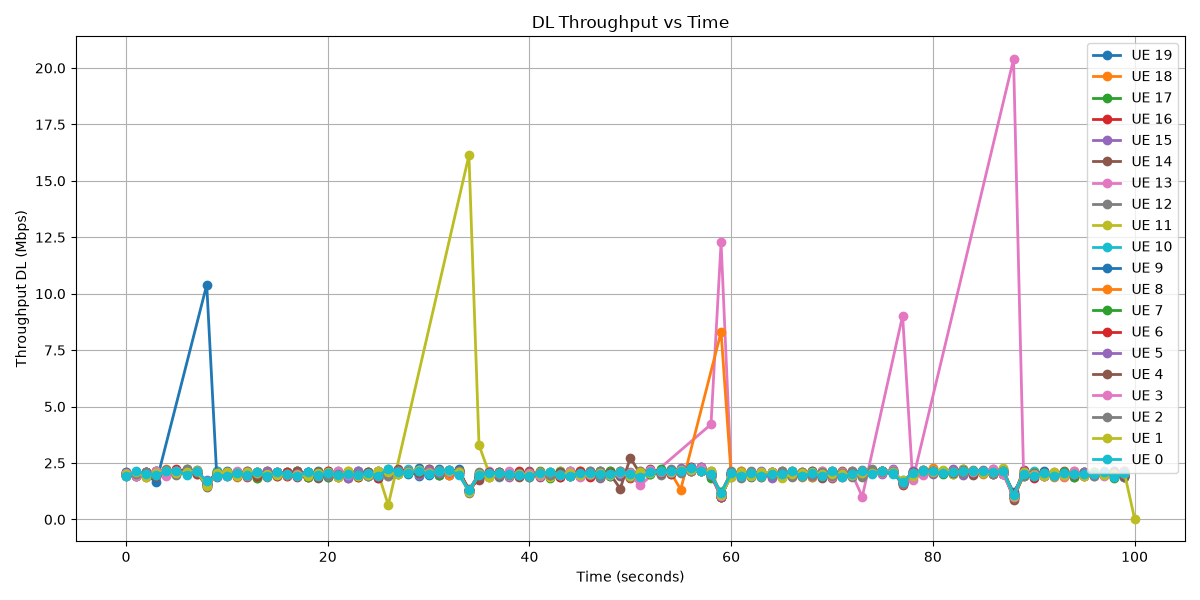
\includegraphics[scale=0.35]{../computos_y_graficas/scheduling_italianos_rma_rapido_pocos_1flujo_pf/5_7_17_33_56/mac/dl_throughput.png}}\end{center}

\begin{center}{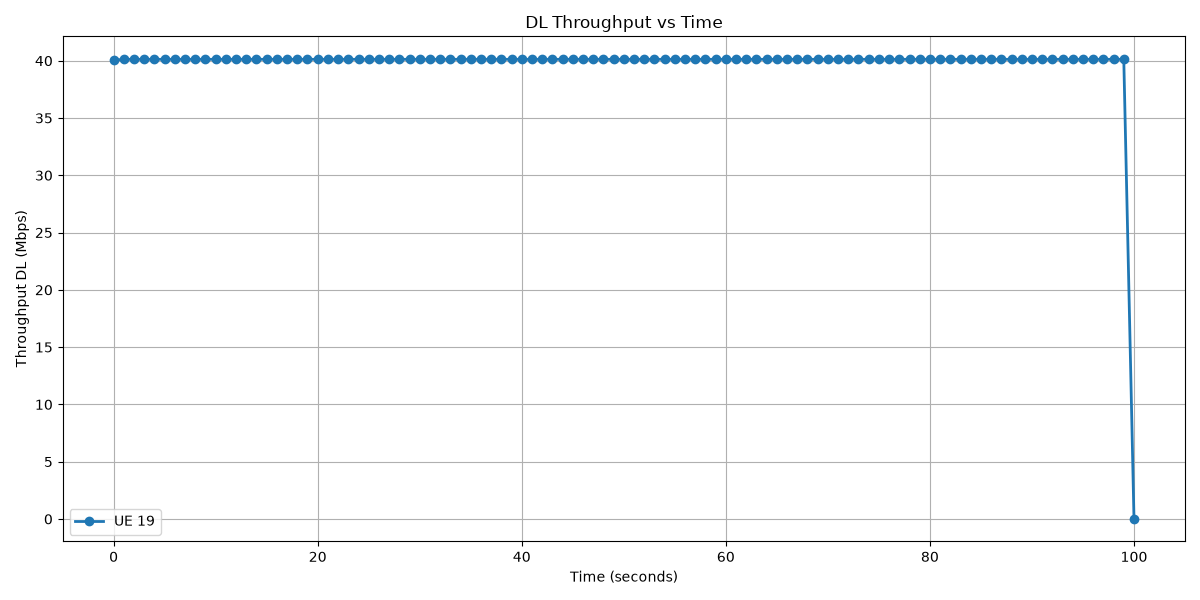
\includegraphics[scale=0.35]{../computos_y_graficas/scheduling_italianos_rma_rapido_pocos_1flujo_mt/5_7_17_23_53/mac/dl_throughput.png}}\end{center}

\begin{center}{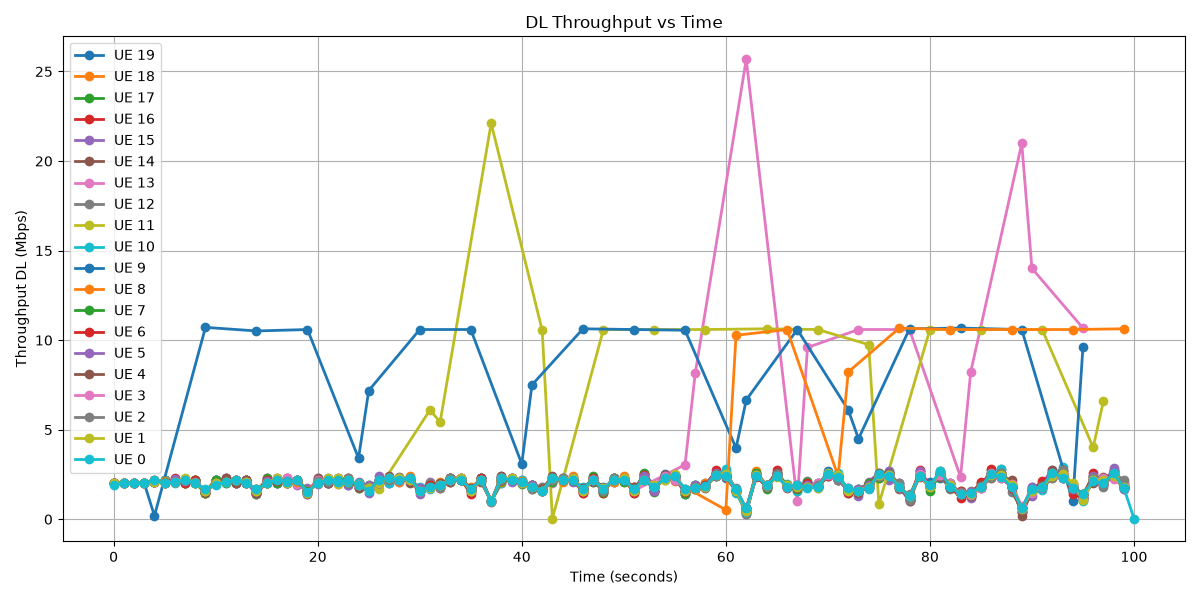
\includegraphics[scale=0.35]{../computos_y_graficas/scheduling_italianos_rma_rapido_pocos_1flujo_lwdf/5_7_17_18_52/mac/dl_throughput.png}}\end{center}

\begin{center}{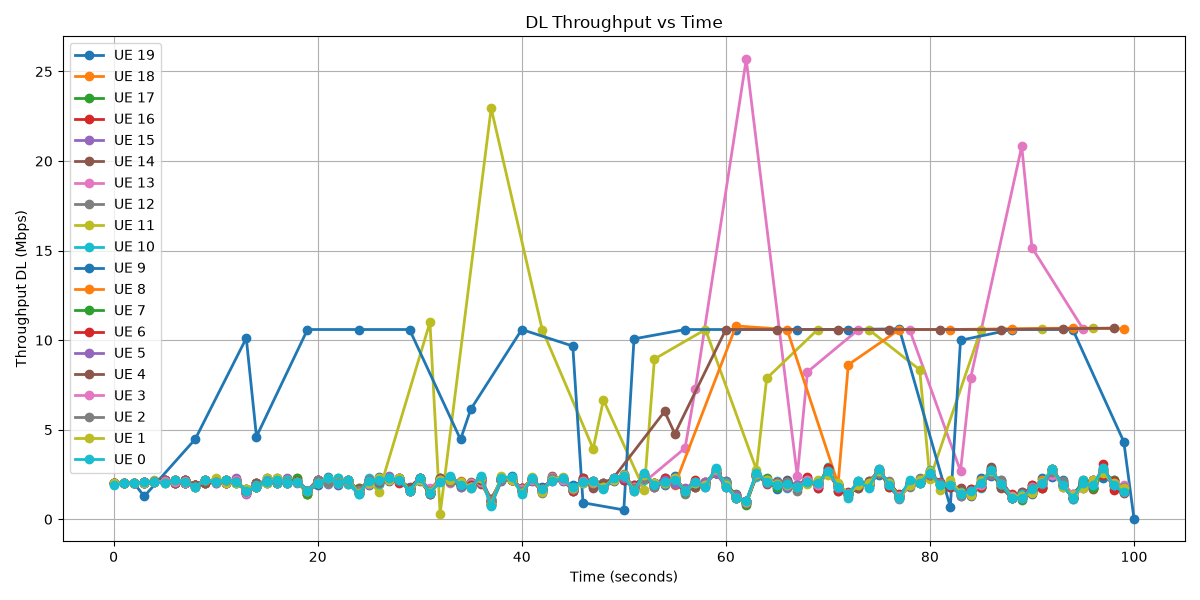
\includegraphics[scale=0.35]{../computos_y_graficas/scheduling_italianos_rma_rapido_pocos_1flujo_fifo/5_7_17_3_47/mac/dl_throughput.png}}\end{center}

\begin{center}{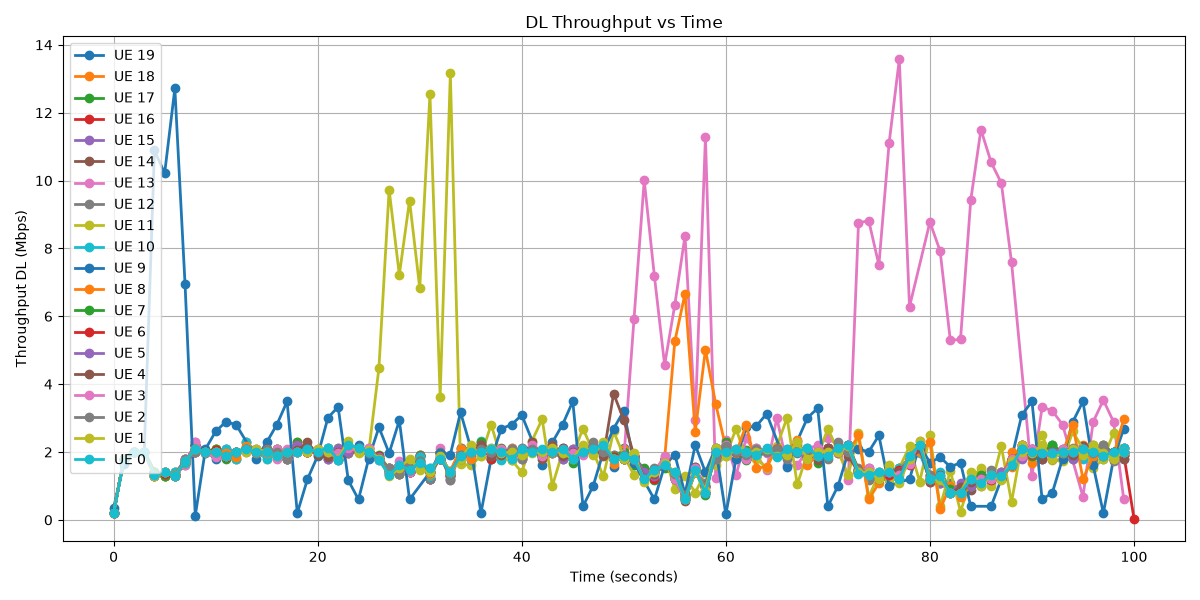
\includegraphics[scale=0.35]{../computos_y_graficas/scheduling_italianos_rma_rapido_pocos_1flujo_edf/5_7_17_13_50/mac/dl_throughput.png}}\end{center}

\begin{figure}[H]
	\ffigbox[\FBwidth] {
	\caption[Planificación de paquetes - Segundo caso - Trazas (I)]{Traza temporal de la tasa de los usuarios para distintas métricas.
	Obtenidas con \textit{FikoRE} en un escenario con 20 UE en una celda RMa (caso \textit{RMa-pocos-un flujo}).

	(Fila 1): RR.

	(Fila 2): PF.

	(Fila 3): MT.

	(Fila 4): LWDF.

	(Fila 5): FIFO.

	(Fila 6): EDF.

	(Fila 7): BET.}
	}
	{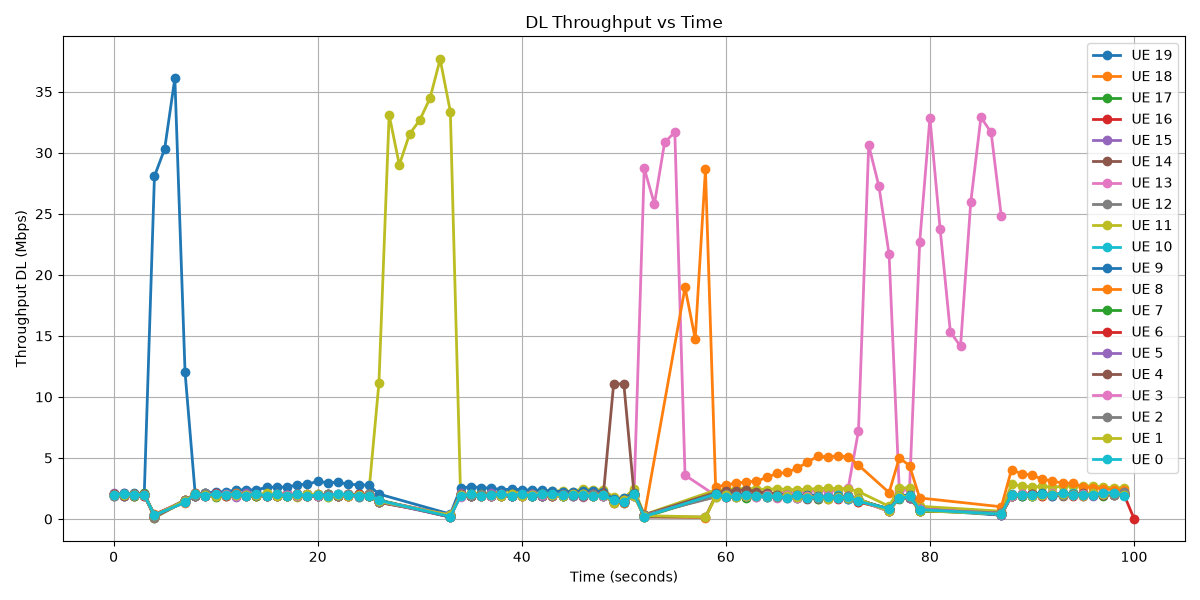
\includegraphics[scale=0.35]{../computos_y_graficas/scheduling_italianos_rma_rapido_pocos_1flujo_bet/5_7_17_8_49/mac/dl_throughput.png}}
\end{figure}

\begin{center}{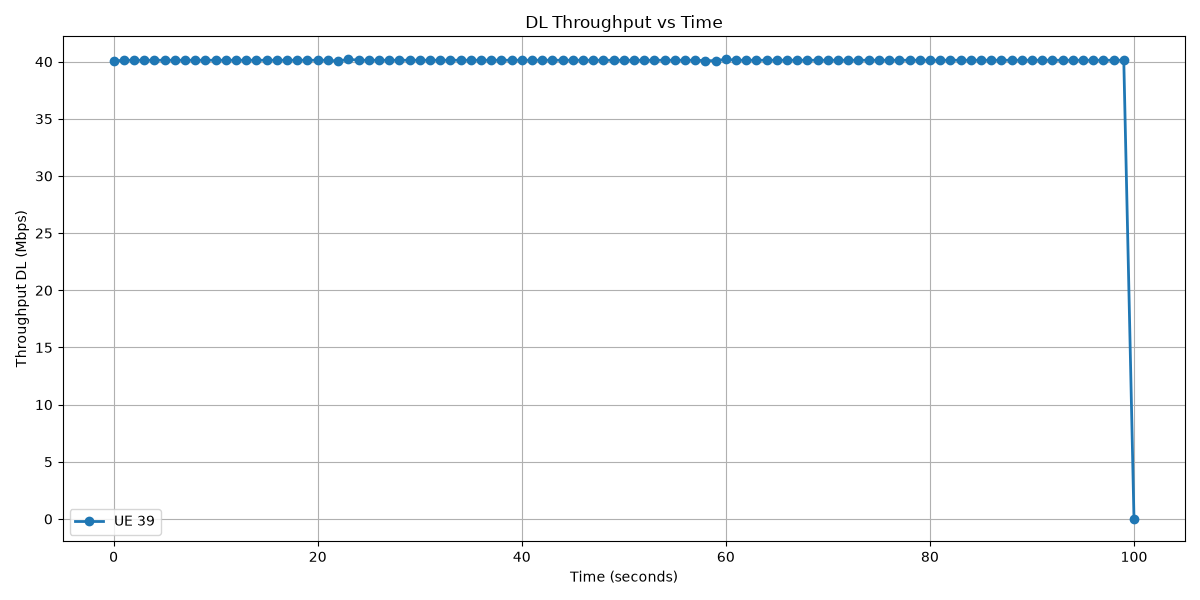
\includegraphics[scale=0.35]{../computos_y_graficas/scheduling_italianos_uma_lento_muchos_1flujo_mt/5_6_21_52_33/mac/dl_throughput.png}}\end{center}

\begin{figure}[H]
	\ffigbox[\FBwidth] {
	\caption[Planificación de paquetes - Segundo caso - Trazas (II)]{Traza temporal de la tasa de los usuarios distintas métricas.
	Obtenidas con \textit{FikoRE} en un escenario con 40 UE en una celda UMa (caso \textit{UMa-muchos-un flujo}).

	(Fila 1): MT.

	(Fila 2): PF.}
	}
	{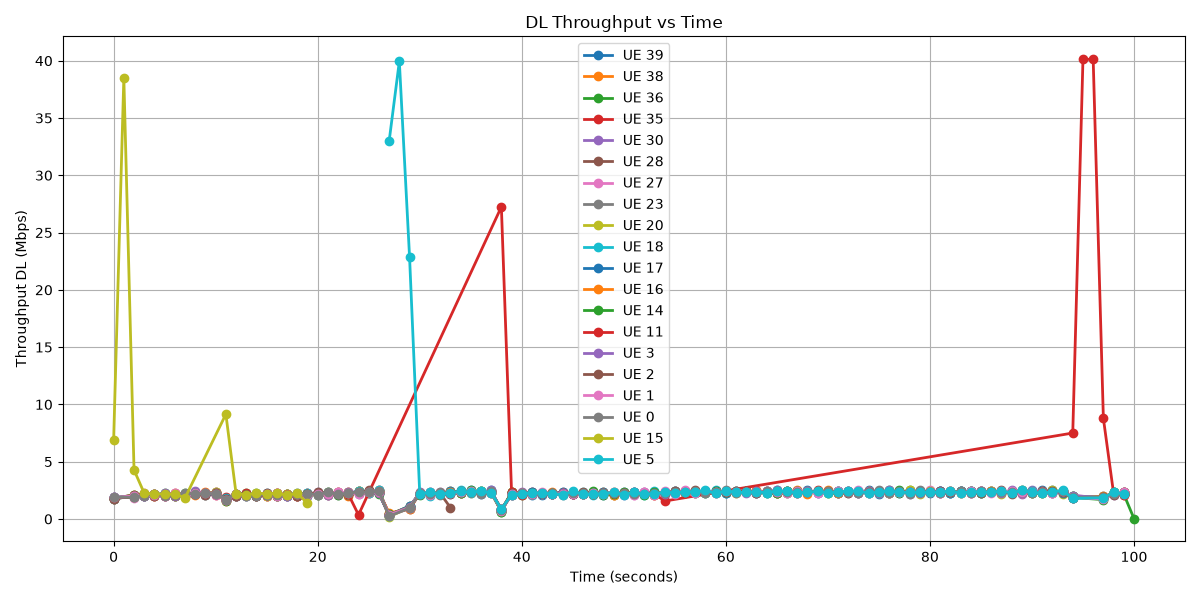
\includegraphics[scale=0.35]{../computos_y_graficas/scheduling_italianos_uma_lento_muchos_1flujo_pf/5_6_22_1_9/mac/dl_throughput.png}}
\end{figure}

\begin{center}{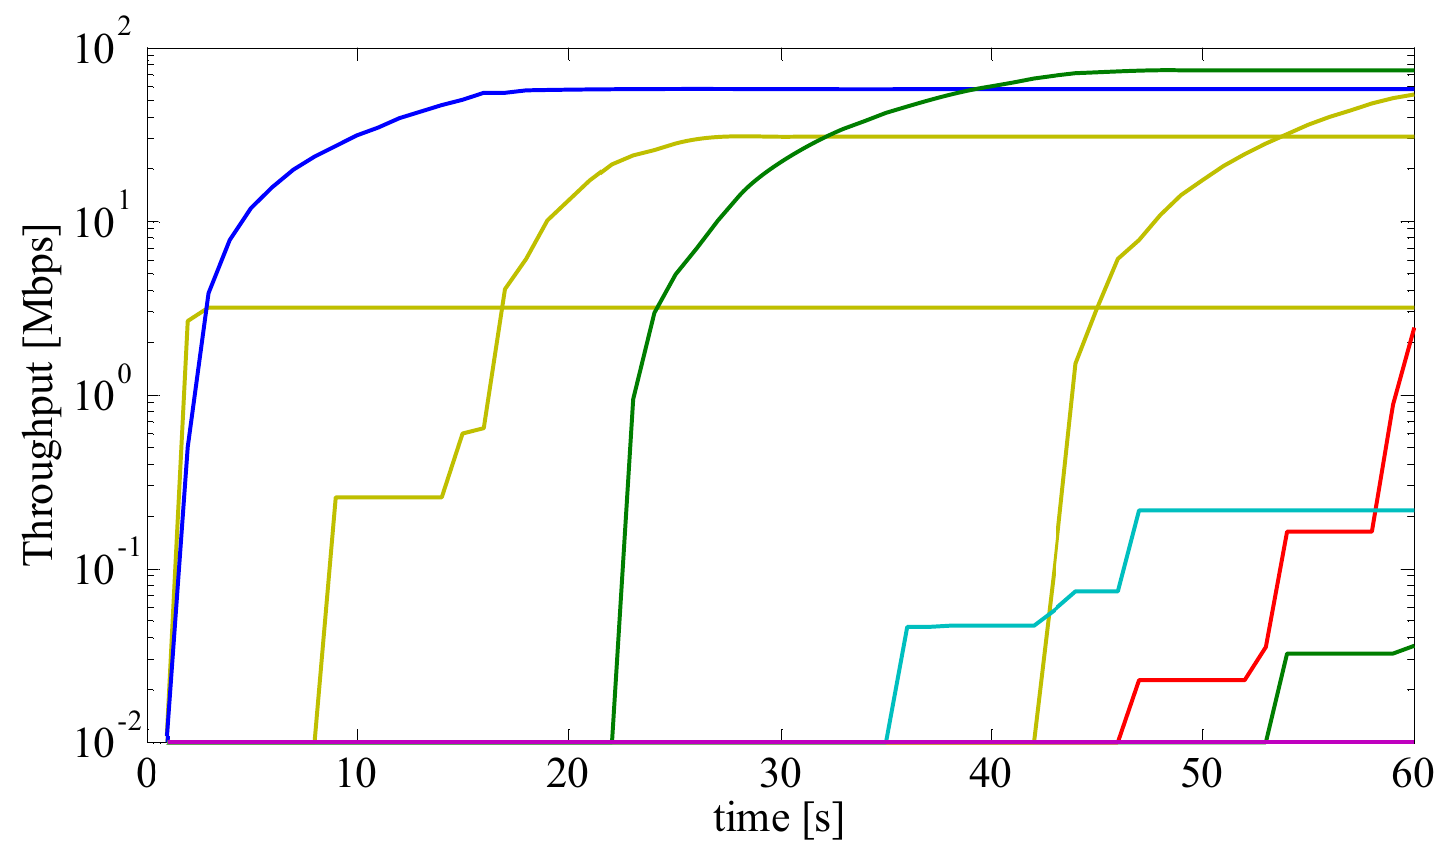
\includegraphics[scale=0.3]{imagenes/scheduling_italianos/scheduling_italianos-202.png}}\end{center}

\begin{figure}[H]
	\ffigbox[\FBwidth] {
	\caption[Planificación de paquetes - Segundo caso - Trazas (III)]{Traza temporal de la tasa de los usuarios para distintas métricas.
	Obtenidas en \cite{RefWorks:26} en un escenario con 40 UE en la celda.

	(Fila 1): MT.

	(Fila 2): PF.}
	}
	{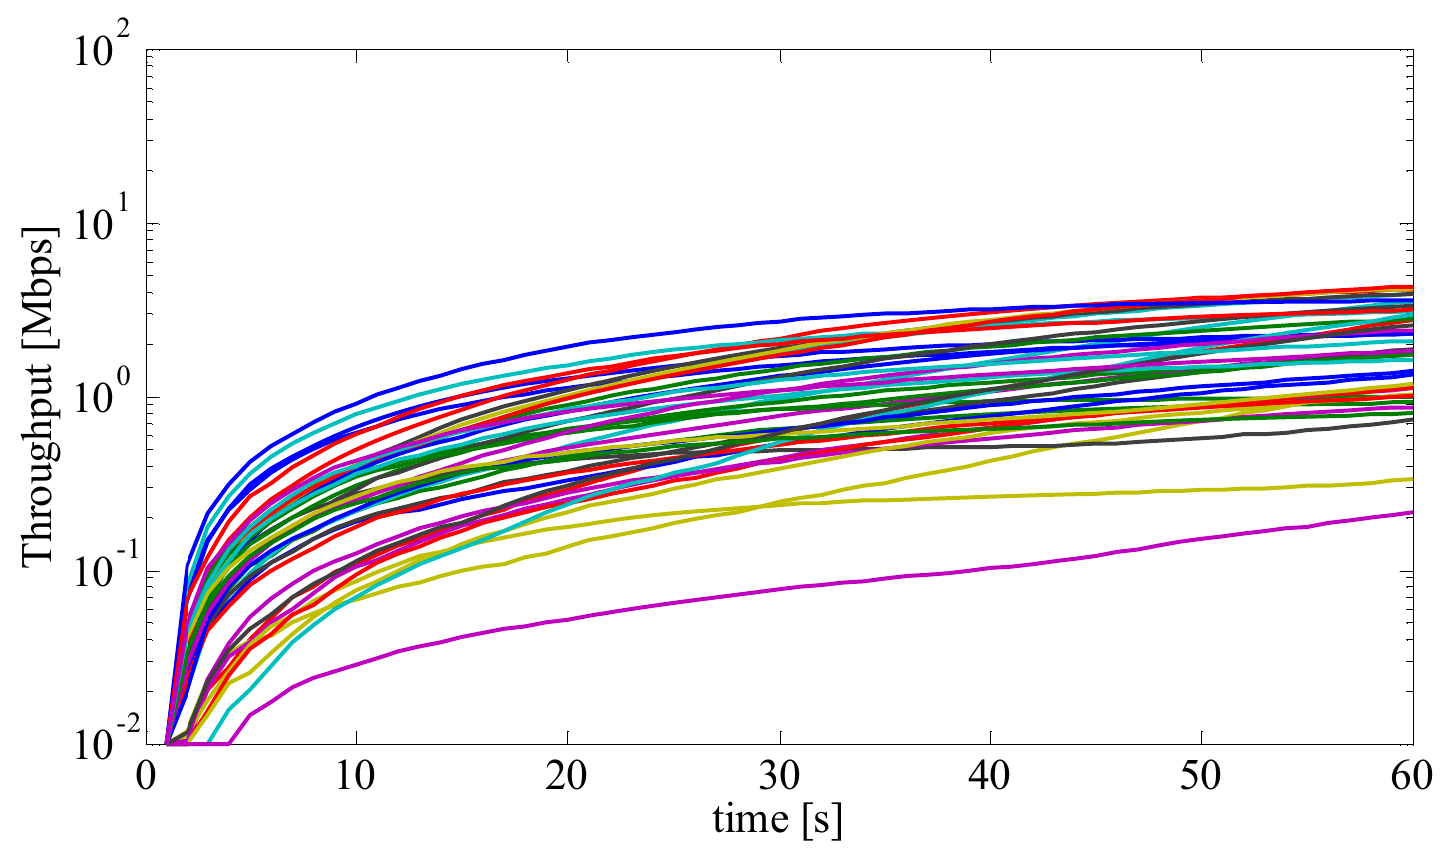
\includegraphics[scale=0.3]{imagenes/scheduling_italianos/scheduling_italianos-203.png}}
\end{figure}

Las conclusiones descritas pueden constatarse también observando el tráfico de cada UE en tiempo real, como se ve en las figura 4.13, 4.14 y 4.15.
La diferencia más evidente entre LTE (figura 4.15) y 5G (figura 4.14) es la velocidad con la que se asignan recursos;
mientras en LTE toma, al menos, cinco segundos que se estabilicen los flujos, en 5G lo hacen casi desde el comienzo.
También se aprecia que en MT logran cursar tráfico muy pocos UE (uno en el caso de 5G) y en PF lo hacen varios.

Si nos centramos en las gráficas con 20 UE, en la figura 4.13, vemos que algunas métricas como LWDF, FIFO y EDF ocasionan muchas irregularidades.
En el caso LWDF y EDF, el comportamiento responde a su diseño para prevenir la expiración de un tiempo límite, lo que hace que repentinamente se asignen recursos a un UE para luego retirárselos;
FIFO atiende a aquellos UE que llevan más tiempo sin ser atendidos, lo que ocasiona asignaciones repentinas.
BET también hace asignaciones repentinas, pues su prioridad está determinada por la tasa que no han logrado cursar los UE sin atender y debe ser restituida en algún momento, ocasionando esas asignaciones.
Por su parte, MT solo atiende al UE con mejor canal.
RR y PF dan un servicio más regular.

\subsubsection{Descripción del experimento 2: \textit{tres flujos}}


En la segunda experiencia, se hace un análisis de las métricas M-LWDF, EXP/PF, \textit{EXP rule}, \textit{LOG rule} y FLS, tomándose como referencia la métrica PF.
Los parámetros del experimento son idénticos al anterior con la salvedad del tráfico, que consiste en tres flujos en dirección DL: un vídeo, una transmisión de VoIP y un flujo de mejor esfuerzo (datos).

Se ha adaptado el mismo experimento para realizarse con el emulador \textit{FikoRE}:

\begin{itemize}
\item Se simula el caso \textit{pocos} (1-20 UE en la celda).
\item Para representar la combinación de tráfico de VoIP, vídeo y datos se ha usado la función de inyección de tráfico de \textit{FikoRE} con una captura de tramas IP reales del mismo tipo de datos (caso \textit{tres flujos}).
\item Se simula el caso \textit{RMa} y el caso \textit{UMa}.
\item {
Se han probado las distintas métricas de las que disponía \textit{FikoRE} y una nueva, M-LWDF, introducida en el módulo de métricas:
\begin{itemize}
\item Caso \textit{RMa-pocos-tres flujos}: M-LWDF, PF, BET, EDF, FIFO, LWDF, MT, RR.
\item Caso \textit{UMa-pocos-tres flujos}: M-LWDF, PF.
\end{itemize}
}
\end{itemize}


\begin{figure}[H]
	{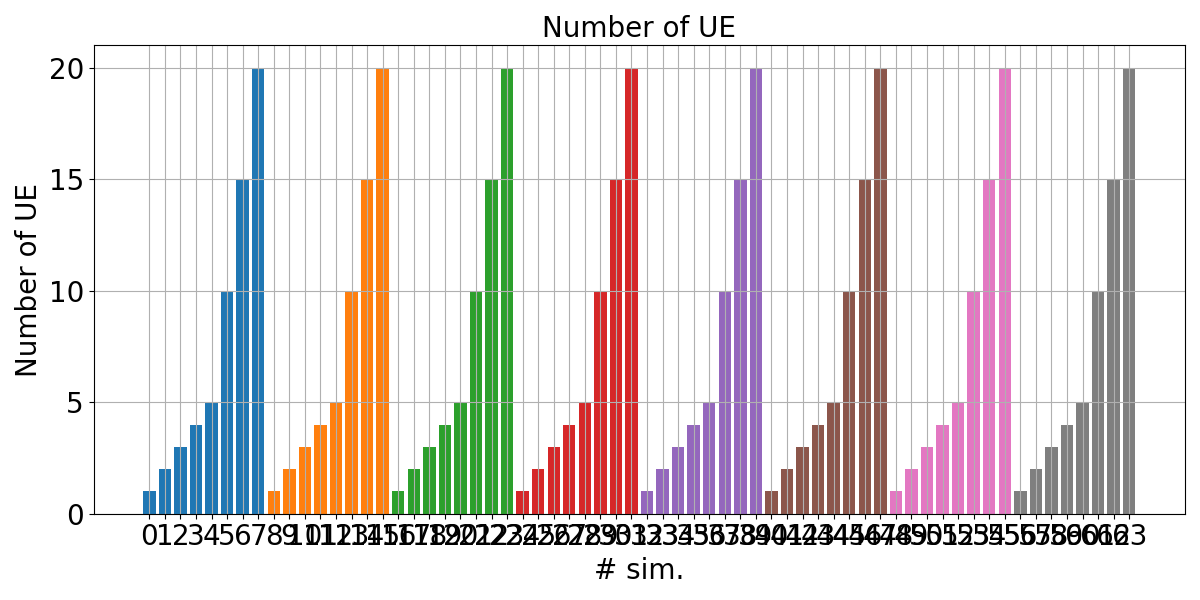
\includegraphics[scale=0.4]{../comparaciones/scheduling_italianos_rma_rapido_3flujo/ue/n_ue_multi_sim.png}}
	\ffigbox[\FBwidth] {
	\caption[Planificación de paquetes - Segundo caso - Nº. de UE (II)]{Número de UE en las distintas simulaciones.

	(Arriba): Caso \textit{RMa-pocos-tres flujos}.
	Las métricas por orden con el número de simulaciones entre paréntesis: M-LWDF (8), PF (8), BET (8), EDF (8), FIFO (8), LWDF (8), MT (8), RR (8).

	(Abajo): Caso \textit{UMa-pocos-tres flujos}.
	Las métricas por orden con el número de simulaciones entre paréntesis: M-LWDF (5), PF (5).}
	}
	{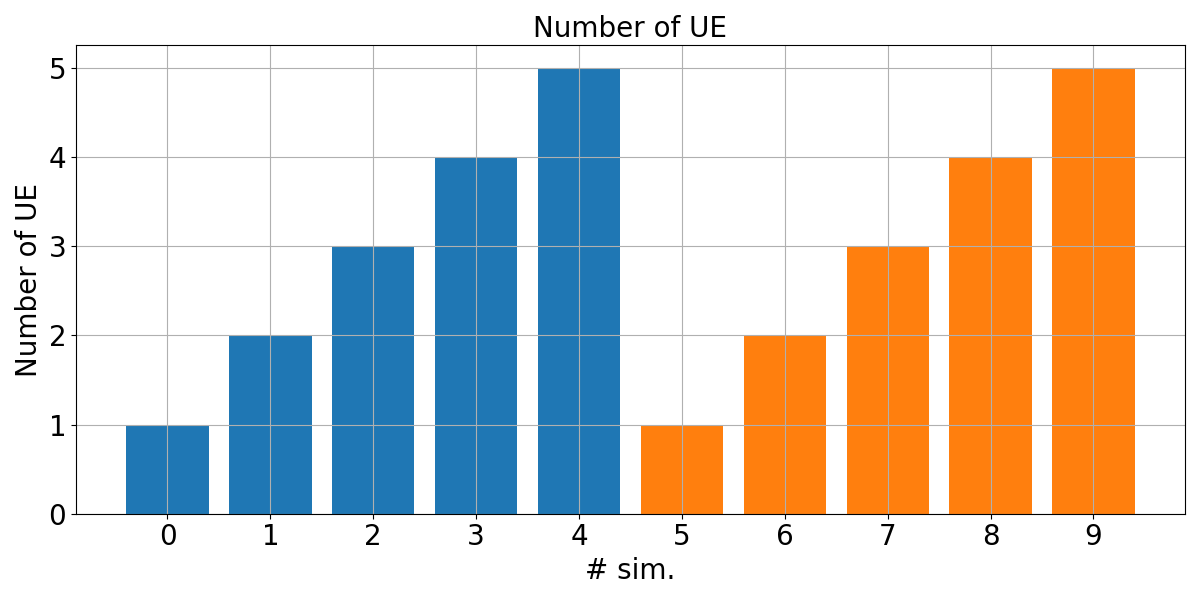
\includegraphics[scale=0.4]{../comparaciones/scheduling_italianos_uma_lento_3flujos/ue/n_ue_multi_sim.png}}
\end{figure}

\subsubsection{Calidad del canal en el experimento 2}

En primer lugar, podemos suponer las mismas prestaciones de la red en lo que respecta a capacidad,
la calidad de los canales de transmisión será la misma que en el anterior experimento, los valores indicativos del estado del canal de transmisión (SINR, RSRP, CQI) serán iguales.

\subsubsection{Prestaciones en el experimento 2}

%La PLR:
%
%\begin{figure}[H]
%	\ffigbox[\FBwidth] {
%	\caption[Caso - Packet scheduling - Italianos)]{AAA}
%	}
%	{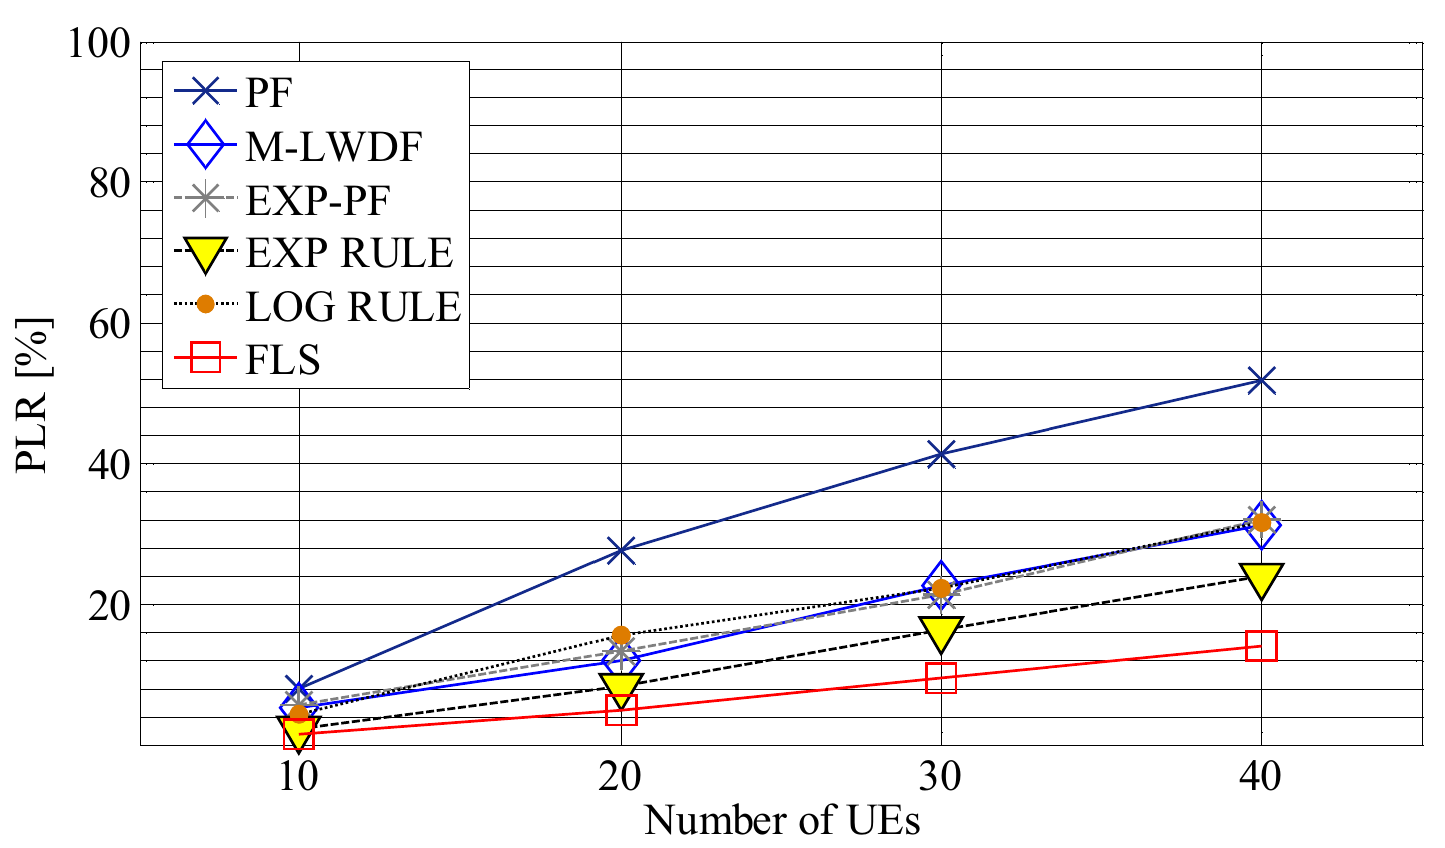
\includegraphics[scale=0.2]{imagenes/scheduling_italianos/scheduling_italianos-206.png}}
%\end{figure}

\begin{center}{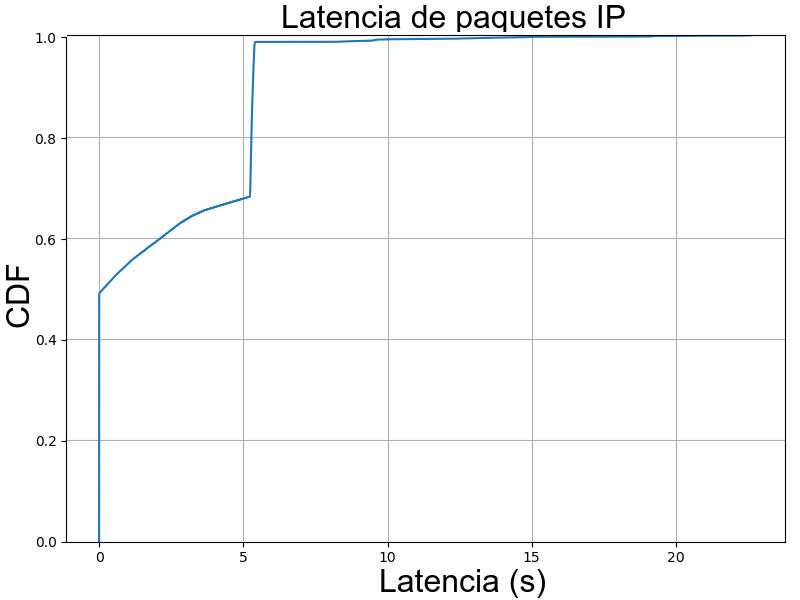
\includegraphics[scale=0.475]{../computos_y_graficas/scheduling_italianos_rma_rapido_pocos_3flujos_rr/8_5_7_11_59_13/ue/cdf_ildl.png_fixed.png}}\end{center}

\begin{center}{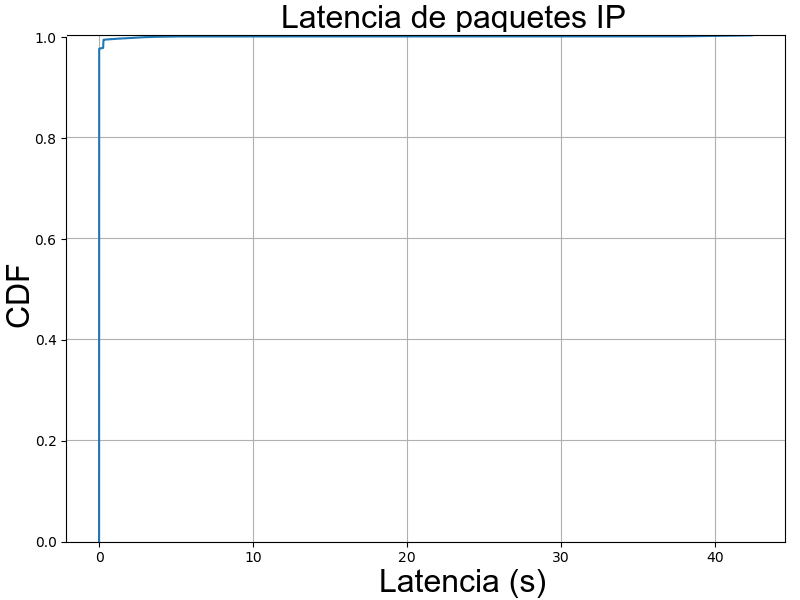
\includegraphics[scale=0.475]{../computos_y_graficas/scheduling_italianos_rma_rapido_pocos_3flujos_mt/5_7_12_13_24/ue/cdf_ildl.png_fixed.png}}\end{center}

\begin{center}{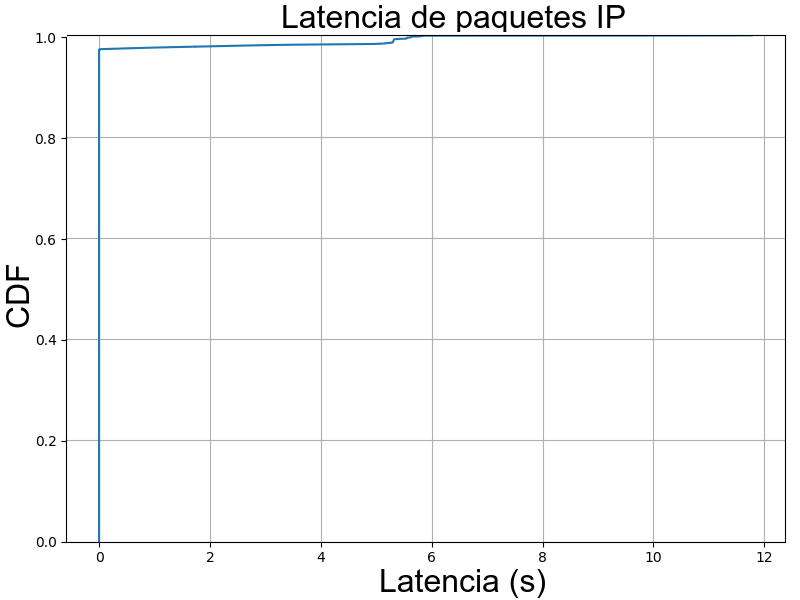
\includegraphics[scale=0.475]{../computos_y_graficas/scheduling_italianos_rma_rapido_pocos_3flujos_lwdf/5_7_11_42_49/ue/cdf_ildl.png_fixed.png}}\end{center}

\begin{center}{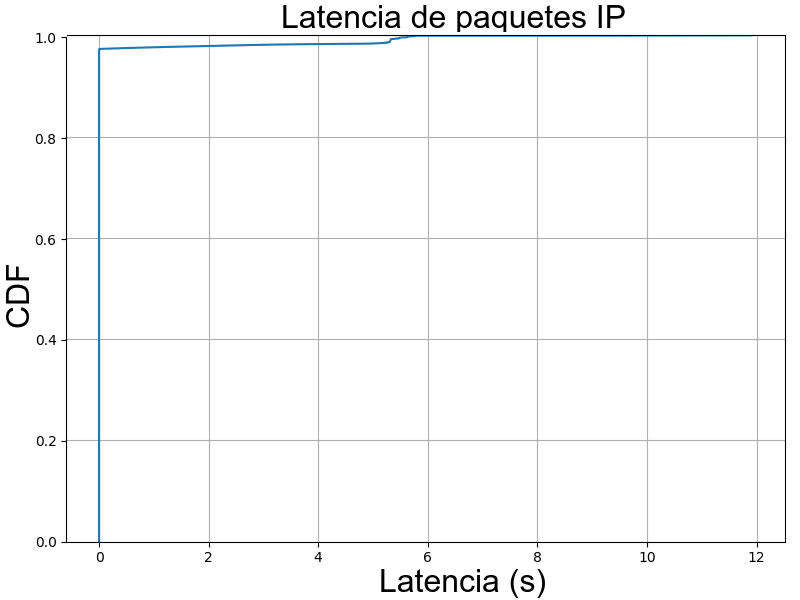
\includegraphics[scale=0.475]{../computos_y_graficas/scheduling_italianos_rma_rapido_pocos_3flujos_fifo/5_7_10_52_14/ue/cdf_ildl.png_fixed.png}}\end{center}

\begin{center}{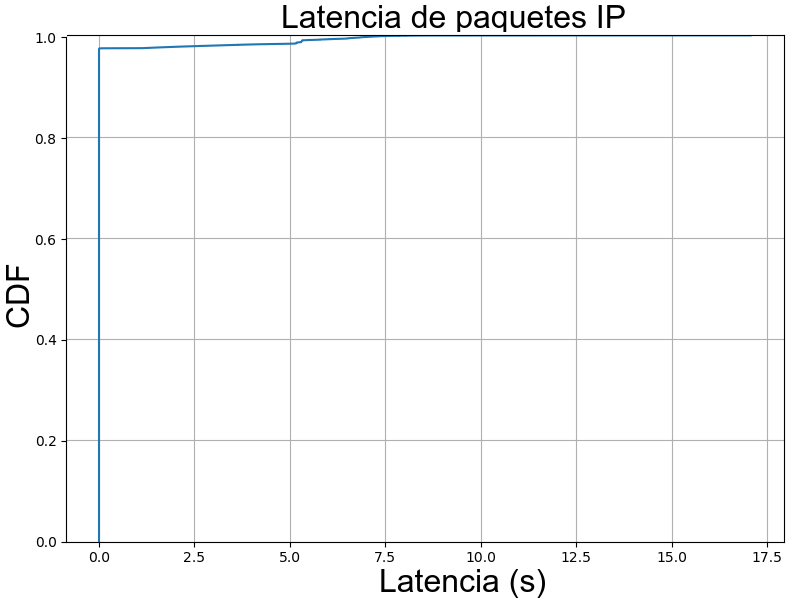
\includegraphics[scale=0.475]{../computos_y_graficas/scheduling_italianos_rma_rapido_pocos_3flujos_edf/5_7_11_29_27/ue/cdf_ildl.png_fixed.png}}\end{center}

\begin{center}{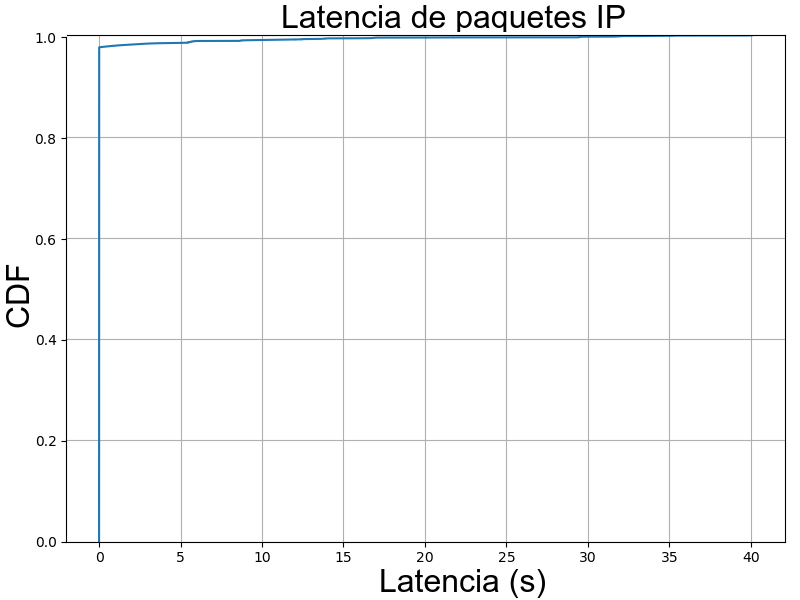
\includegraphics[scale=0.475]{../computos_y_graficas/scheduling_italianos_rma_rapido_pocos_3flujos_bet/8_5_7_11_13_52/ue/cdf_ildl.png_fixed.png}}\end{center}

\begin{center}{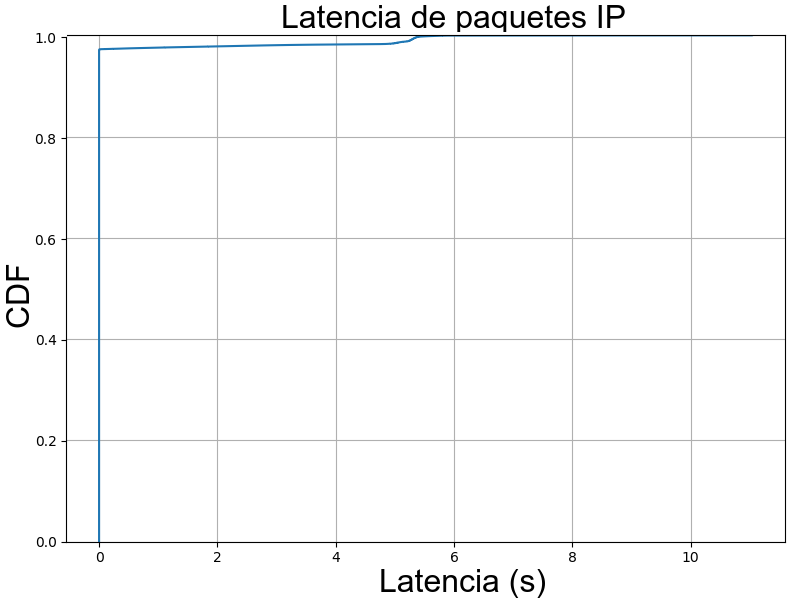
\includegraphics[scale=0.475]{../computos_y_graficas/scheduling_italianos_rma_rapido_pocos_3flujo_pf/5_7_13_15_13/ue/cdf_ildl.png_fixed.png}}\end{center}

\begin{figure}[H]
	\ffigbox[\FBwidth] {
	\caption[Planificación de paquetes - Segundo caso - Latencia (I)]{CDF de la latencia de los paquetes IP para distintas métricas.
	Obtenidas con \textit{FikoRE} en una celda RMa (caso \textit{RMa-pocos-tres flujos}).

	(Fila 1): RR.

	(Fila 2): MT.

	(Fila 3): LWDF.

	(Fila 4): FIFO.

	(Fila 5): EDF.

	(Fila 6): BET.

	(Fila 7): PF.

	(Fila 8): M-LWDF.}
	}
	{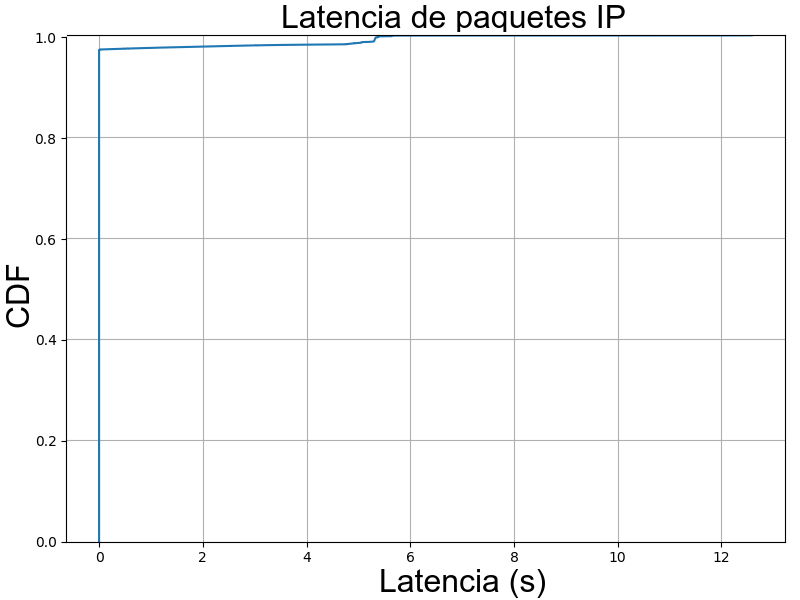
\includegraphics[scale=0.475]{../computos_y_graficas/scheduling_italianos_rma_rapido_pocos_3flujo_mlwdf/5_7_13_25_37/ue/cdf_ildl.png_fixed.png}}
\end{figure}

\begin{figure}[H]
	\ffigbox[\FBwidth] {
	\caption[Planificación de paquetes - Segundo caso - Latencia en el artículo]{CDF del retardo de los paquetes del flujo de vídeo con 20 usuarios en el experimento de \cite{RefWorks:26}.}
	}
	{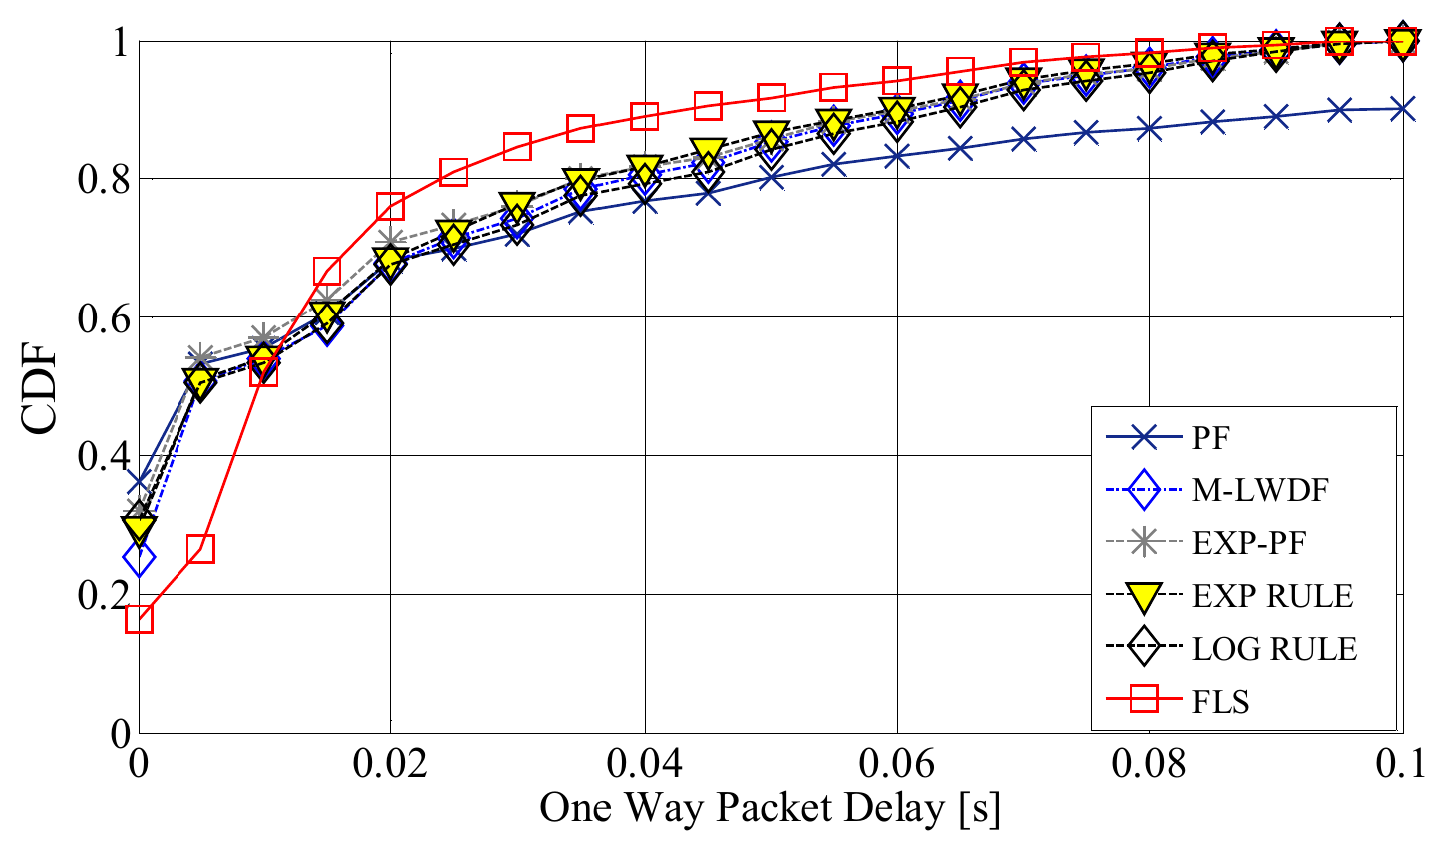
\includegraphics[scale=0.3]{imagenes/scheduling_italianos/scheduling_italianos-208.png}}
\end{figure}

En este experimento, atendemos a aspectos relevantes en los servicios en tiempo real.
La función de distribución acumulada (\textit{cumulative distribution function}, CDF) de la latencia de los paquetes IP para los casos de 20 UE se muestra en las figuras 4.17 y 4.18.
Se puede observar que RR en particular y las métricas que no están diseñadas con criterios de QoS (MT, LWDF, FIFO, EDF, BET, PF) dan lugar a latencias grandes.
Por el contrario, las métricas con QoS (M-LWDF) garantiza la entrega del paquete en un tiempo razonable (0.1 s),
debiéndose a que se descartan los paquetes que excenden el tiempo límite.
En particular, M-LWDF garantiza un equilibrio entre eficiencia espectral, justicia y QoS.
\cite{RefWorks:26}
Se concluye lo mismo que en \cite{RefWorks:26}, las métricas sin QoS no se pueden usar para servicios que requieran poca latencia.

\begin{center}{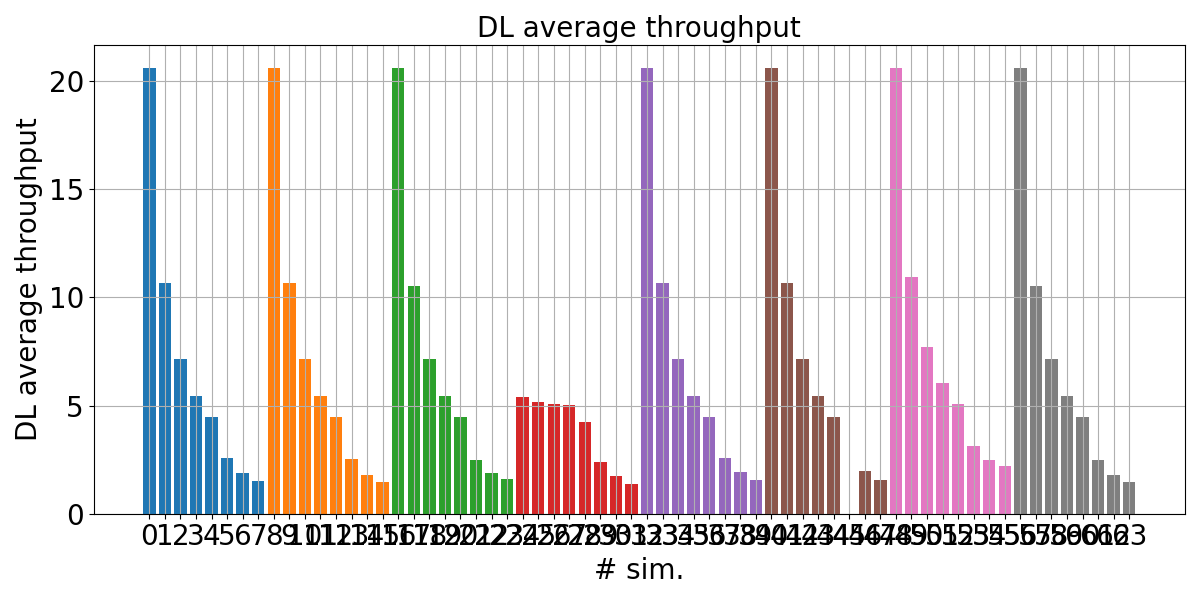
\includegraphics[scale=0.4]{../comparaciones/scheduling_italianos_rma_rapido_3flujo/ue/dl_ave_throughput_multi_sim.png}}\end{center}

\begin{center}{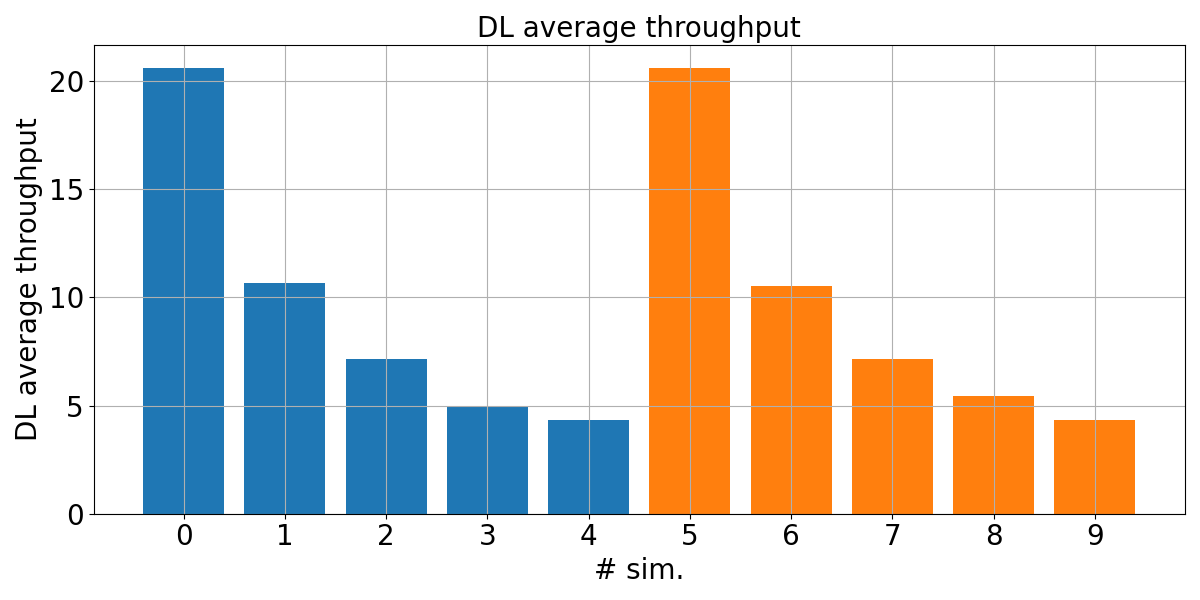
\includegraphics[scale=0.4]{../comparaciones/scheduling_italianos_uma_lento_3flujos/ue/dl_ave_throughput_multi_sim.png}}\end{center}

\begin{figure}[H]
	\ffigbox[\FBwidth] {
	\caption[Planificación de paquetes - Segundo caso - Tasa binaria por UE (III)]{Tasa binaria de un UE en promedio.

	(Fila 1): Caso \textit{RMa-pocos-tres flujos}.
	Las métricas por orden con el número de simulaciones entre paréntesis: M-LWDF (8), PF (8), BET (8), EDF (8), FIFO (8), LWDF (8), MT (8), RR (8).

	(Fila 2): Caso \textit{UMa-pocos-tres flujos}.
	Las métricas por orden con el número de simulaciones entre paréntesis: M-LWDF (5), PF (5).

	(Fila 3): Resultados de \cite{RefWorks:26}.}
	}
	{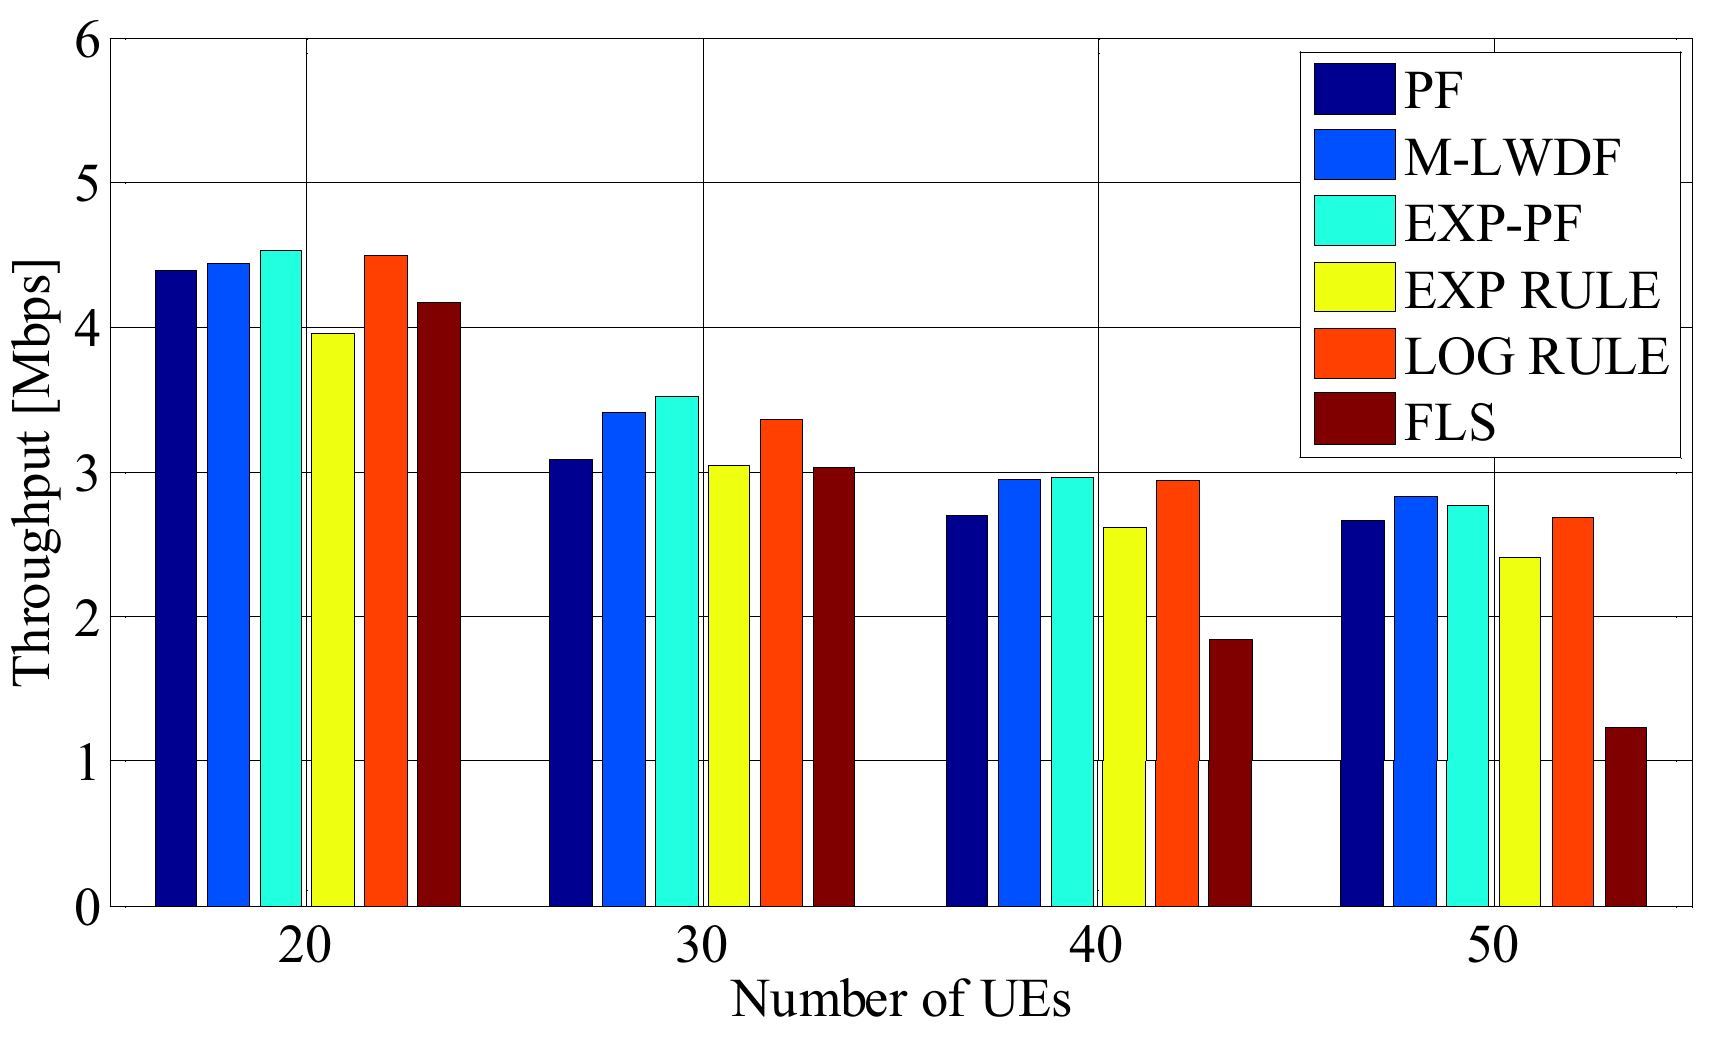
\includegraphics[scale=0.2]{imagenes/scheduling_italianos/scheduling_italianos-211.png}}
\end{figure}

En la figura 4.19 se ve la tasa de UE promedio.
En primer lugar, si bien las simulaciones con \textit{FikoRE} no son comparables a las mostradas en \cite{RefWorks:26} por usarse un número de UE distinto,
en el caso de 20 UE, que sí se ha realizado con los dos simuladores,
se puede ver que la métrica M-LWDF no destaca en cuanto a tasa binaria con respecto al resto,
en el caso de la UMa, es casi igual en prestaciones a PF;
como se indicó, está diseñada para garantizar un equilibrio entre eficiencia espectral, justicia y QoS.
En el caso de la celda RMa, con 20 UE se da menos tasa que en LTE, pero con la celda UMa se iguala.
Si ahora nos fijamos en las diferencias entre métricas, todas dan prestaciones similares de tasa en el rango de UE simulado salvo EDF;
por los mismos motivos explicados en el anterior experimento, esta métrica no ofrece tasas grandes incluso con pocos UE.

\subsection{Planificación de paquetes para URLLC}

\subsubsection{Introducción}

El artículo \cite{RefWorks:66} se centra en el servicio URLLC de 5G.
Describe un experimento en el que se analizan las métricas más relevantes para el mismo.
Se analizan de manera cuantitativa usando una metodología de nivel de sistema.
La metodología descrita sigue las especificaciones de 3GPP para NR.
Incluye muchas funcionalidades:
despliegues con varias celda, modelos de tráfico de usuario dinámico, modelos de canal en tres dimensiones, la pila de protocolos de 5G NR, planificación de paquetes, adaptación de enlace, HARQ, MIMO en transmisión y en recepción, etc.

El objetivo es estudiar las prestaciones con la planificación de paquetes en varias celdas al mismo tiempo (\textit{multi-cell scheduling}),
en contraste con la planificación llevada a cabo en cada celda por separado (\textit{distributed scheduling}), como la que hasta ahora hemos presentado con \textit{FikoRE}.
También estudian las prestaciones de usar una RAN centralizada (C-RAN),
en lugar de una en la que cada interfaz sea manejada por su celda, que es como se hace en \textit{FikoRE}.
Adicionalmente, añaden una métrica basada en M-LWDF llamada \textit{TP-Delay};
adaptando la notación de \cite{RefWorks:66} a la de \cite{RefWorks:26}:
$$
m_{i, k}^{TP-Delay} = \left\lbrace
\begin{array}{lr}
d_{k}^i (t) \quad si \quad D_{HOL, i} \leq \mathsf{0.5 \quad ms} \\
D_{HOL, i} \cdot \frac {d_{k}^i (t)} { \psi } \quad si \quad D_{HOL, i} > \mathsf{0.5 \quad ms}
\end{array}
\right.
$$
Se pretende así estudiar la viabilidad del servicio URLLC.
\cite{RefWorks:66}

Se ha representado el experimento con \textit{FikoRE}
(véase \textit{Caso de uso (VIII): packet scheduling (daneses)} en el anexo \textit{Simulaciones (metadatos)}).

\subsubsection{Descripción del experimento}

Si bien \textit{FikoRE} no incluye todas las funcionalidades mostradas en \cite{RefWorks:66},
el artículo muestra simulaciones de escenarios que sí puede representar \textit{FikoRE},
la comparación es posible y nos permite contrastar la metodología de \cite{RefWorks:66} con \textit{FikoRE}.
Las características del experimento se resumen en la tabla 4.2.

% \begin{figure}[H]
% 	\ffigbox[\FBwidth] {
% 	\caption[Caso - Packet scheduling - Daneses]{Características del experimento propuesto en \cite{RefWorks:66}.}
% 	}
% 	{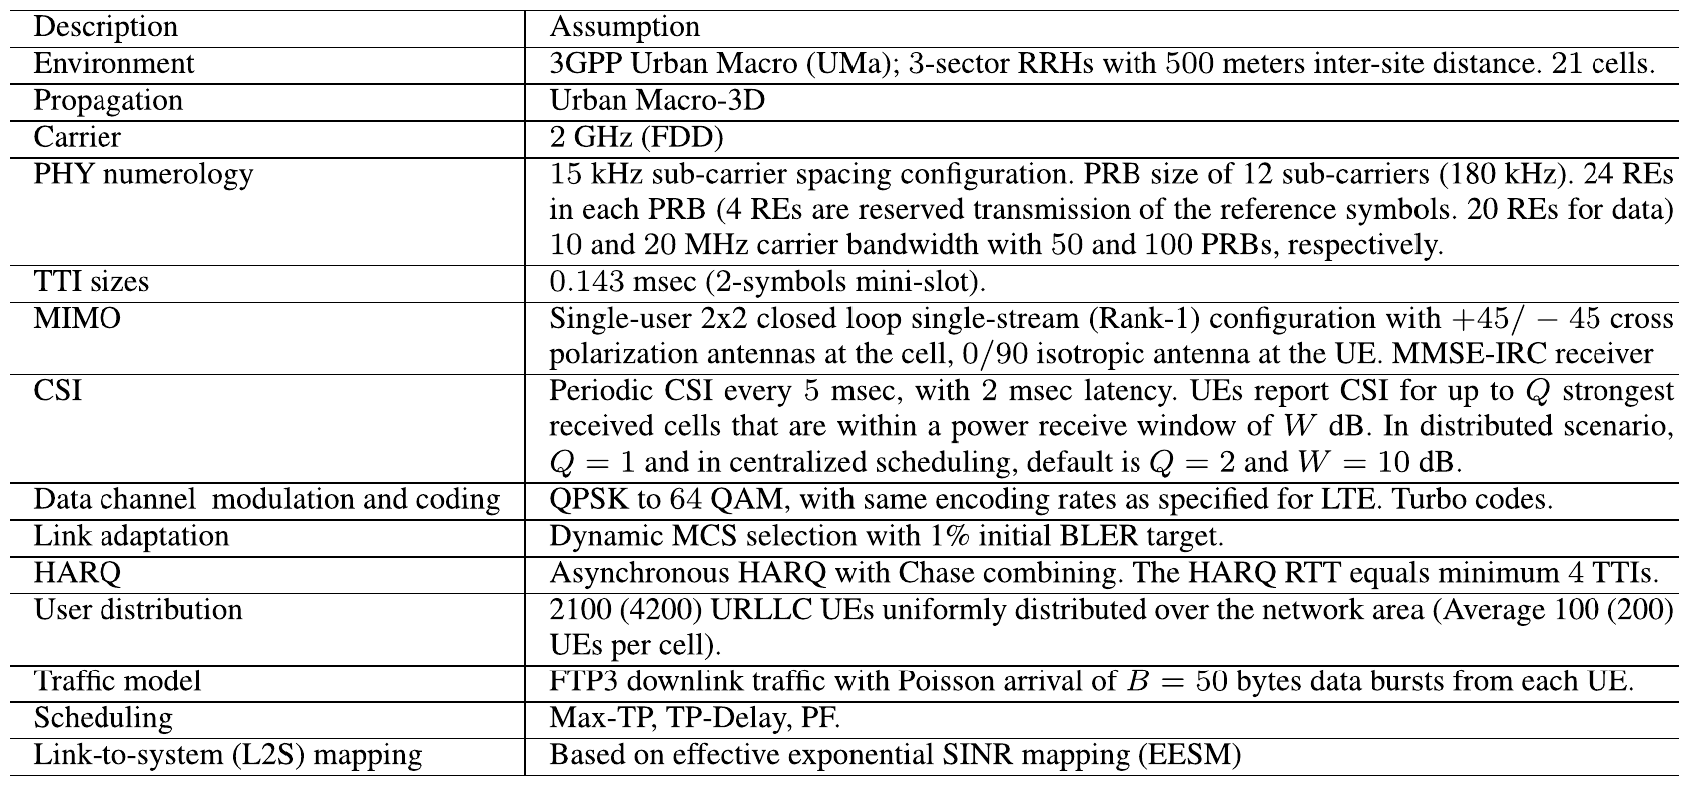
\includegraphics[scale=0.35]{imagenes/scheduling_daneses/scheduling_daneses-004.png}}
% \end{figure}

\begin{table}[H]
	\ttabbox[\FBwidth]
	{\caption{Planificación de paquetes - Tercer caso - Características del experimento propuesto}}
	{\begin{tabular}{|P{3.0cm}|P{10cm}|}
		\hline
		\textbf{Parámetro} & \textbf{Valor} \\
		\hline
		Entorno &
		Macrocelda urbana (UMa);
		RRH de tres sectores con separación de 500 m entre sitios;
		21 celdas \\
		\hline
		Propagación &
		Modelo tridimensional de macrocelda urbana (UMa) \\
		\hline
		Portadora &
		2 GHz;
		FDD \\
		\hline
		Numerología &
		Espaciado entre subportadoras: 15 kHz;
		Tamaño de PRB: 12 subportadoras de 180 kHz;
		PRB: 24 RE (cuatro RE están reservados para la transmisión de símbolos de referencia, 20 RE se usan para transmitir datos);
		Ancho de banda: 10 MHz (50 PRB), 20 MHz (100 PRB) \\
		\hline
		Tamaño de TTI &
		0.143 ms (\textit{minislot} de dos símbolos) \\
		\hline
		MIMO &
		Configuración (celda): Flujo único con bucle cerrado de $2 \times 2$ para usuario único (\textit{Rank-1});
		Polarización (celda: polarización cuzada $+45 / -45$;
		Antena del UE: Antena isotrópica 0/90;
		Estimador: MMSE-IRC \\
		\hline
		CSI &
		Período de notificación: 5 ms;
		Latencia: 2 ms;
		Mecanismo: Cada UE notifica su CSI a un número de hasta $Q$ celdas, las que mejor se perciben y que se encuentren en una ventana de potencia recibida de $W$ dB;
		Casos: En escenario distribuido, $Q = 1$, en planificación centralizada, $Q = 2$ por defecto y $W = 10$ dB \\
		\hline
		Modulación y codificación del canal de datos &
		De QPSK a 64-QAM, con las mismas tasas de codificación que LTE. Se usan turbocódigos. \\
		\hline
		Adaptación de enlace &
		Mecanismo: Selección dinámica de MCS;
		Objetivo de BLER: 1\% \\
		\hline
		HARQ &
		Mecanismo: HARQ asíncrono con combinación Chase;
		Período: RTT de duración de un mínimo de 4 TTI \\
		\hline
		Usuarios &
		Número: 2100, 4200;
		Distribución: Uniformemente distribuidos en el área de la celda (100 ó 200 por celda, en promedio) \\
		\hline
		Servicio &
		URLLC \\
		\hline
		Tráfico & En cada UE, tráfico de FTP3 en DL en forma de ráfagas de 50 bytes con distribución de Poisson \\
		\hline
		Planificador &
		MT, PF, \textit{TP-Delay} \\
		\hline
		Link-to-System (L2S) &
		Basado en SINR exponencial efectivo (EESM) \\
		\hline
		\multicolumn{2}{l}{Fuente: \cite{RefWorks:66}}
	\end{tabular}}
\end{table}

Se ha adaptado el mismo experimento para realizarse con el emulador \textit{FikoRE}:

\begin{itemize}
\item Al no moder representarse varias celdas, se ha reducido el experimento a una celda
con la misma densidad de UE por celda, es decir, 100 UE y 200 UE.
\item Para representar el tráfico de datos de 3.5 Mbps por celda, se ha generado un tráfico de
0.035 Mbps en ambas direcciones, UL y DL, en cada UE.
\item Se han probado las distintas métricas de las que disponía \textit{FikoRE} y otra introducida: FIFO, BET, EDF, LWDF, MT, RR, PF, M-LWDF.
\end{itemize}

\begin{center}{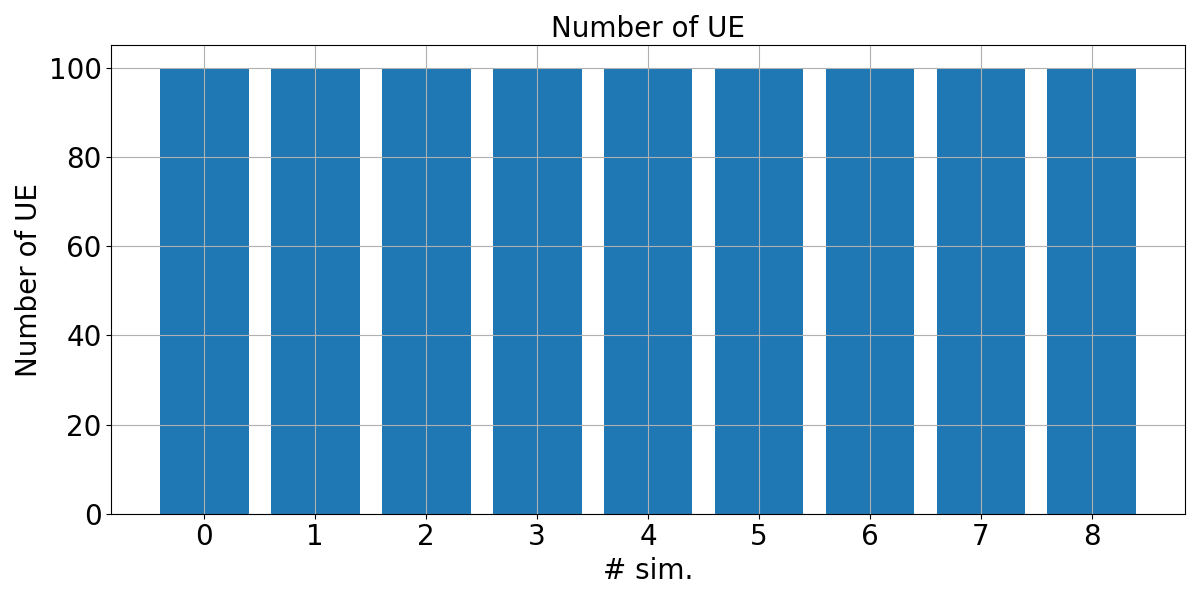
\includegraphics[scale=0.4]{../comparaciones/scheduling_daneses_10mhz_3.5mbps_100ue/ue/n_ue_multi_sim.png}}\end{center}

\begin{figure}[H]
	\ffigbox[\FBwidth] {
	\caption[Planificación de paquetes - Tercer caso - Nº. de UE (I)]{Número de UE en las distintas simulaciones.

	(Arriba): Simulaciones con 100 UE.
	Las métricas por orden: FIFO, BET, EDF, LWDF, MT, RR, PF, M-LWDF.

	(Abajo): Simulaciones con 200 UE.
	Las métricas por orden: FIFO, BET, EDF, LWDF, MT, RR, PF, M-LWDF.}
	}
	{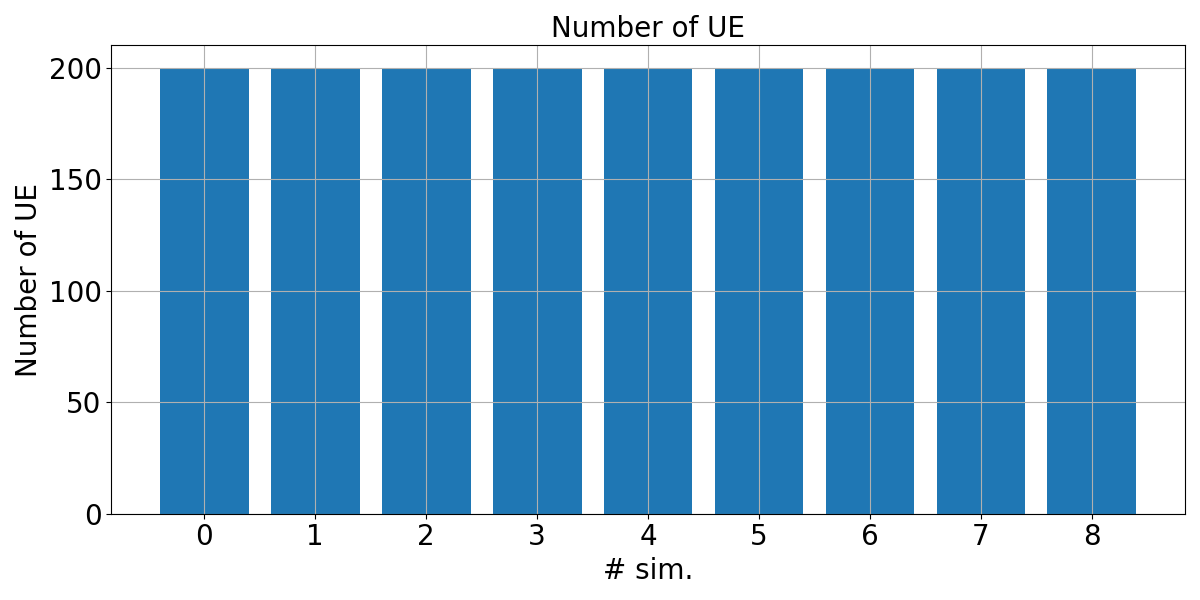
\includegraphics[scale=0.4]{../comparaciones/scheduling_daneses_10mhz_3.5mbps_200ue/ue/n_ue_multi_sim.png}}
\end{figure}

\subsubsection{Calidad del canal}

De manera idéntica al epígrafe anterior, podemos prever que las prestaciones de tasa binaria de la red están limitadas por el ancho de banda, el ruido y la interferencia.
Suponiendo una SINR de 200, resultaba una tasa máxima de 76,511 Mbps.

\begin{center}{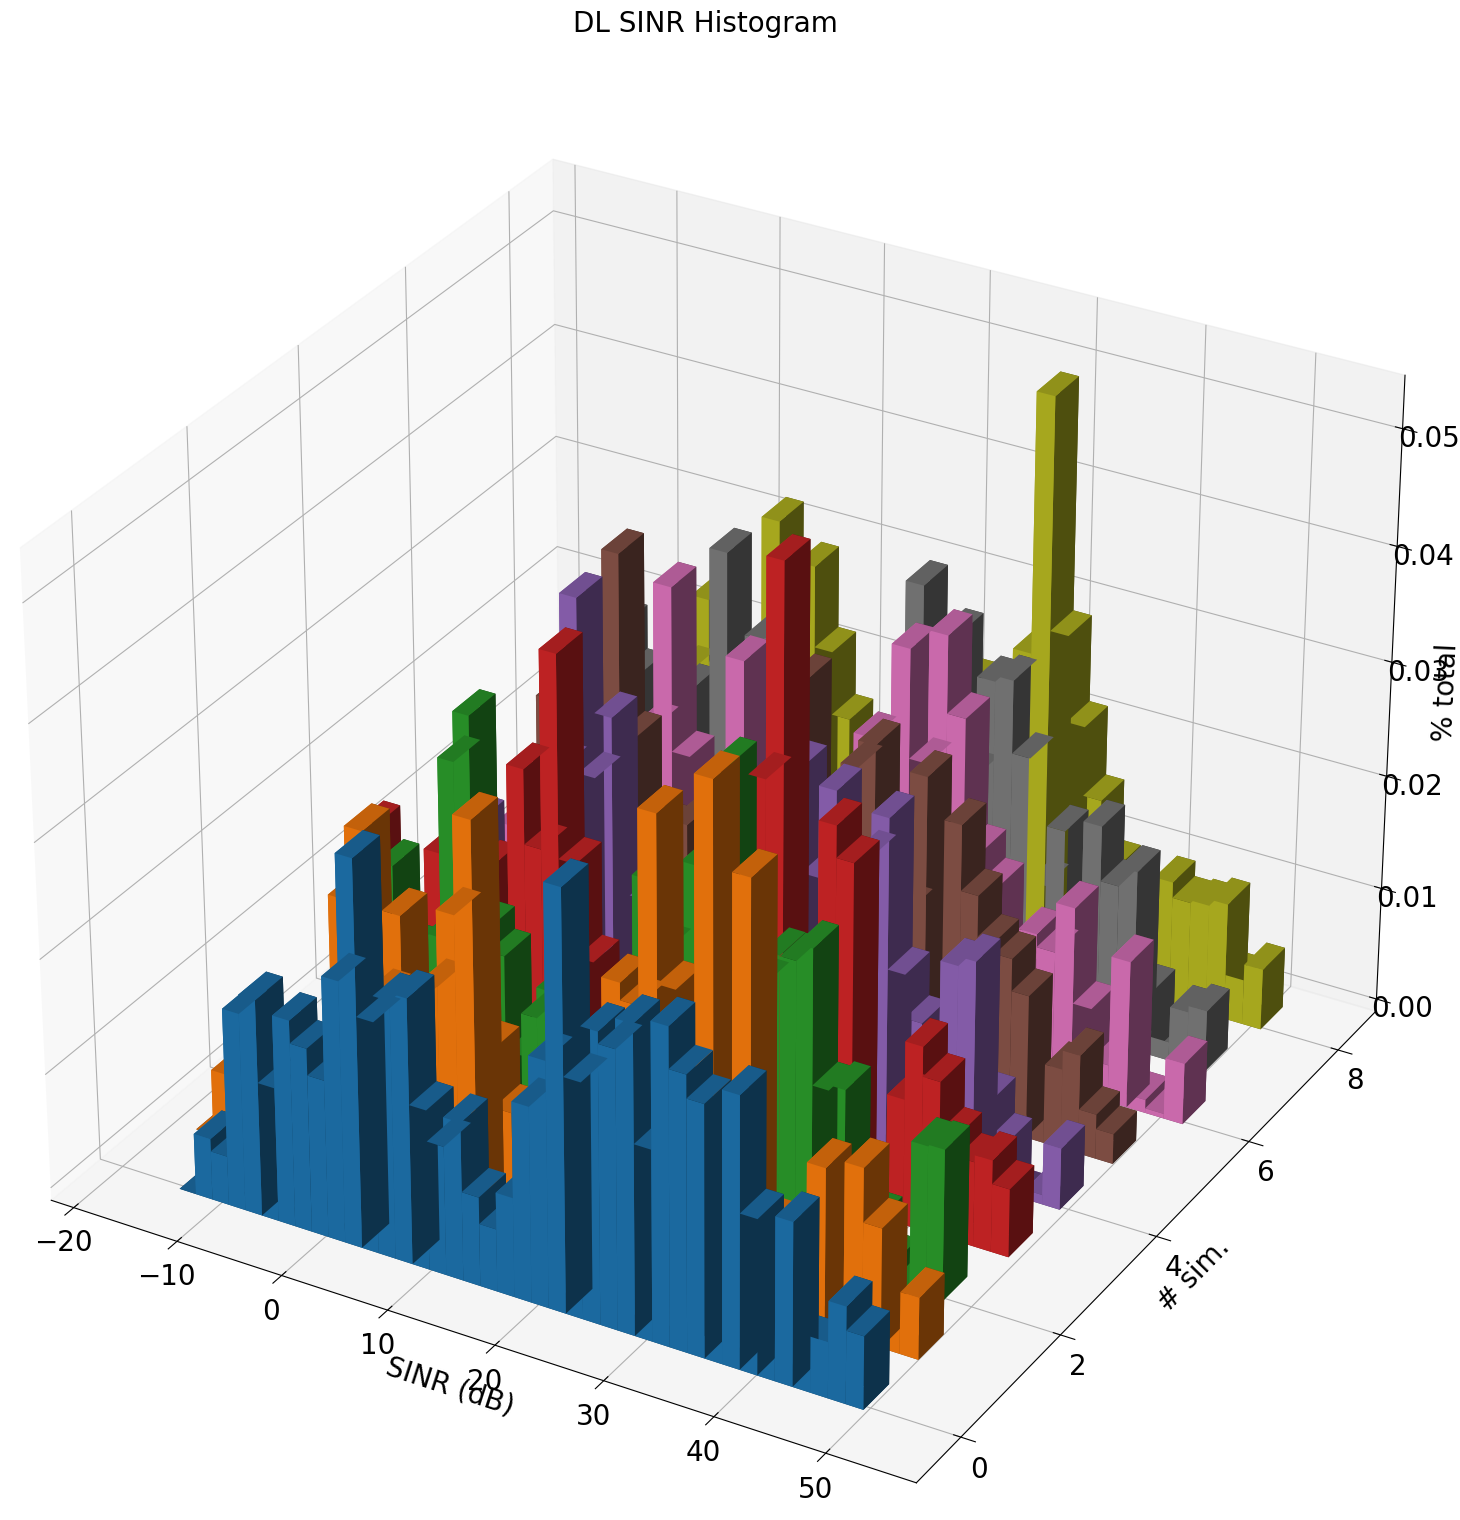
\includegraphics[scale=0.42]{../comparaciones/scheduling_daneses_10mhz_3.5mbps_100ue/ue/sinr_dl_3d_hist_all_ue_multi.png_cropped.png}}\end{center}

\begin{center}{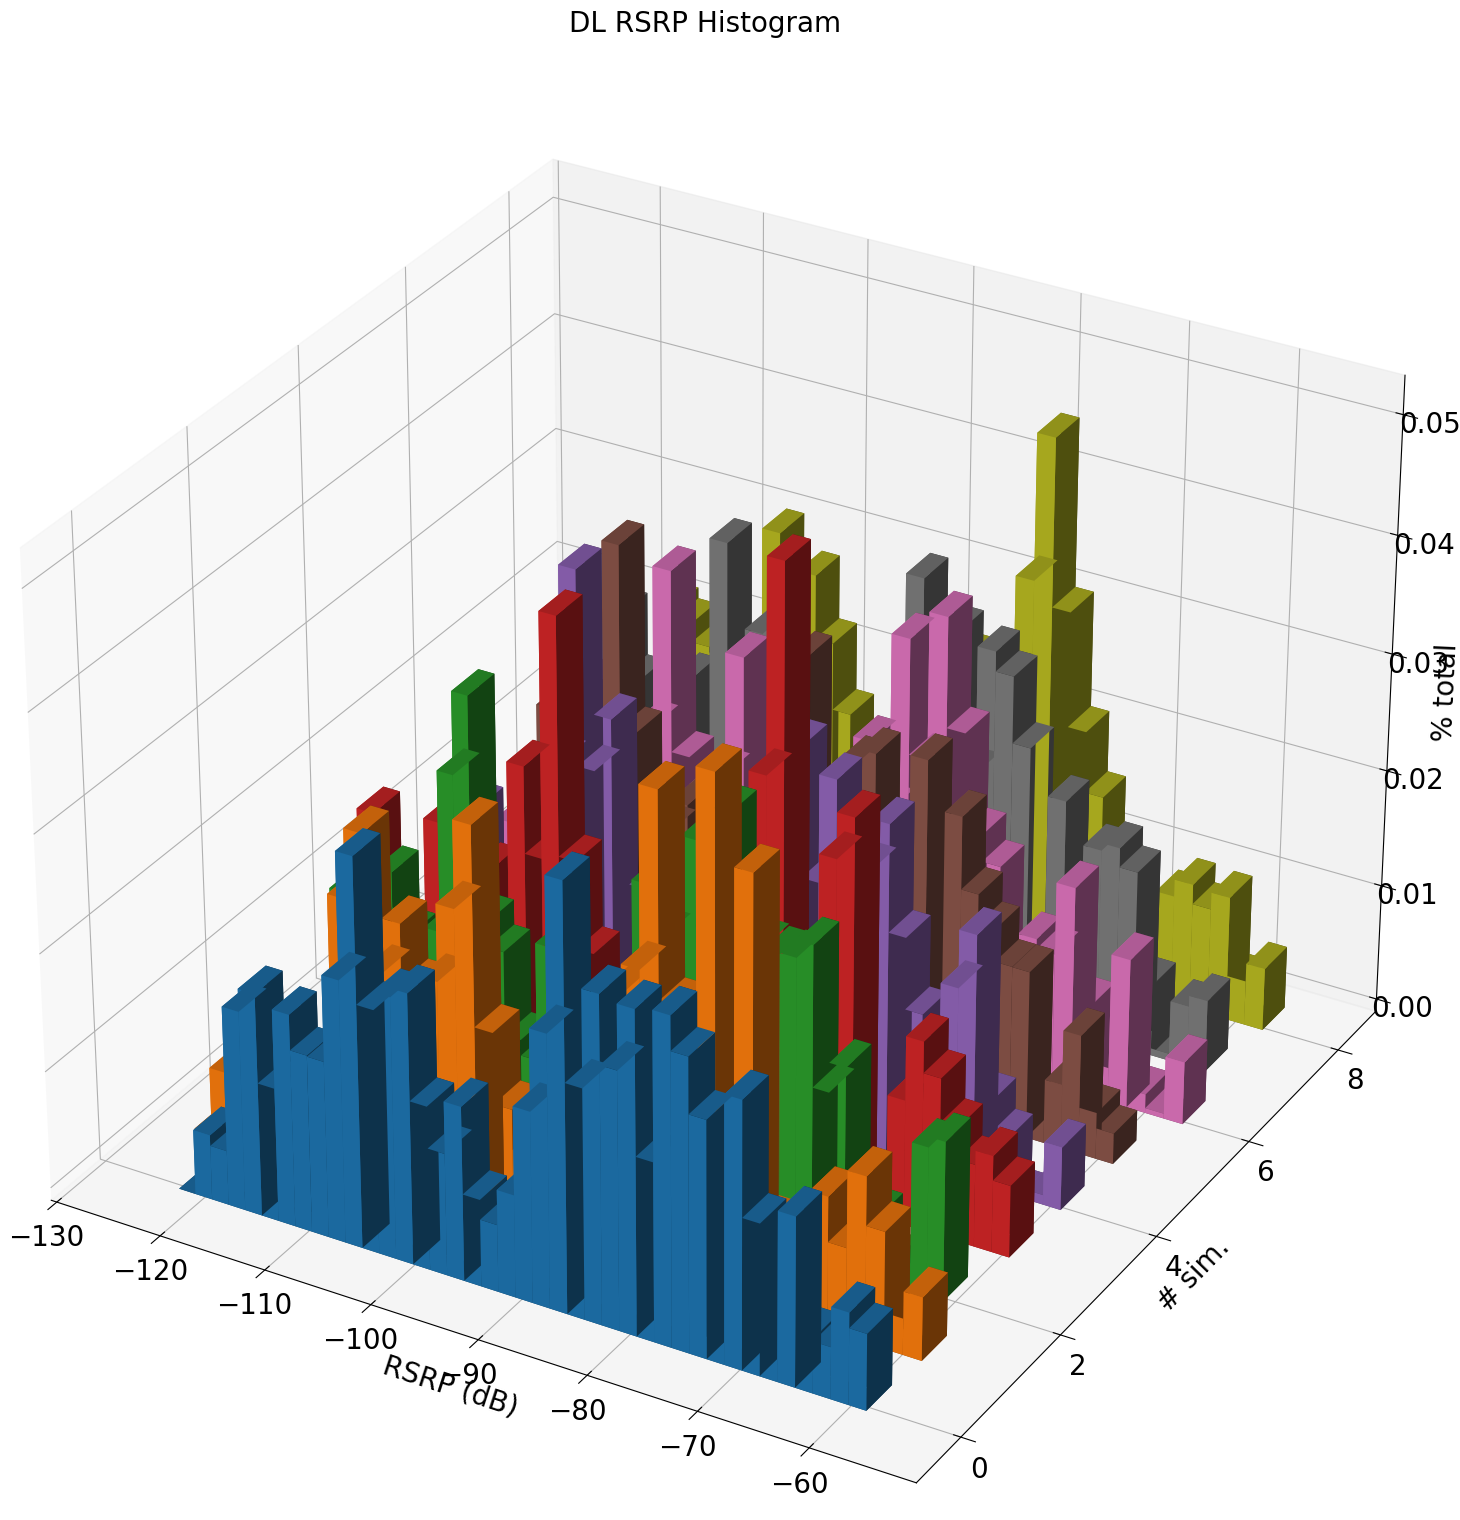
\includegraphics[scale=0.42]{../comparaciones/scheduling_daneses_10mhz_3.5mbps_100ue/ue/rsrp_dl_3d_hist_all_ue_multi.png_cropped.png}}\end{center}

\begin{figure}[H]
	\ffigbox[\FBwidth] {
	\caption[Planificación de paquetes - Tercer caso - Canal (I)]{Distribuciones de los indicadores del estado de canal para la dirección DL.

	Las métricas por orden: FIFO, BET, EDF, LWDF, MT, RR, PF, M-LWDF.

	(Fila 1): SINR.

	(Fila 2): RSRP.

	(Fila 3): CQI.}
	}
	{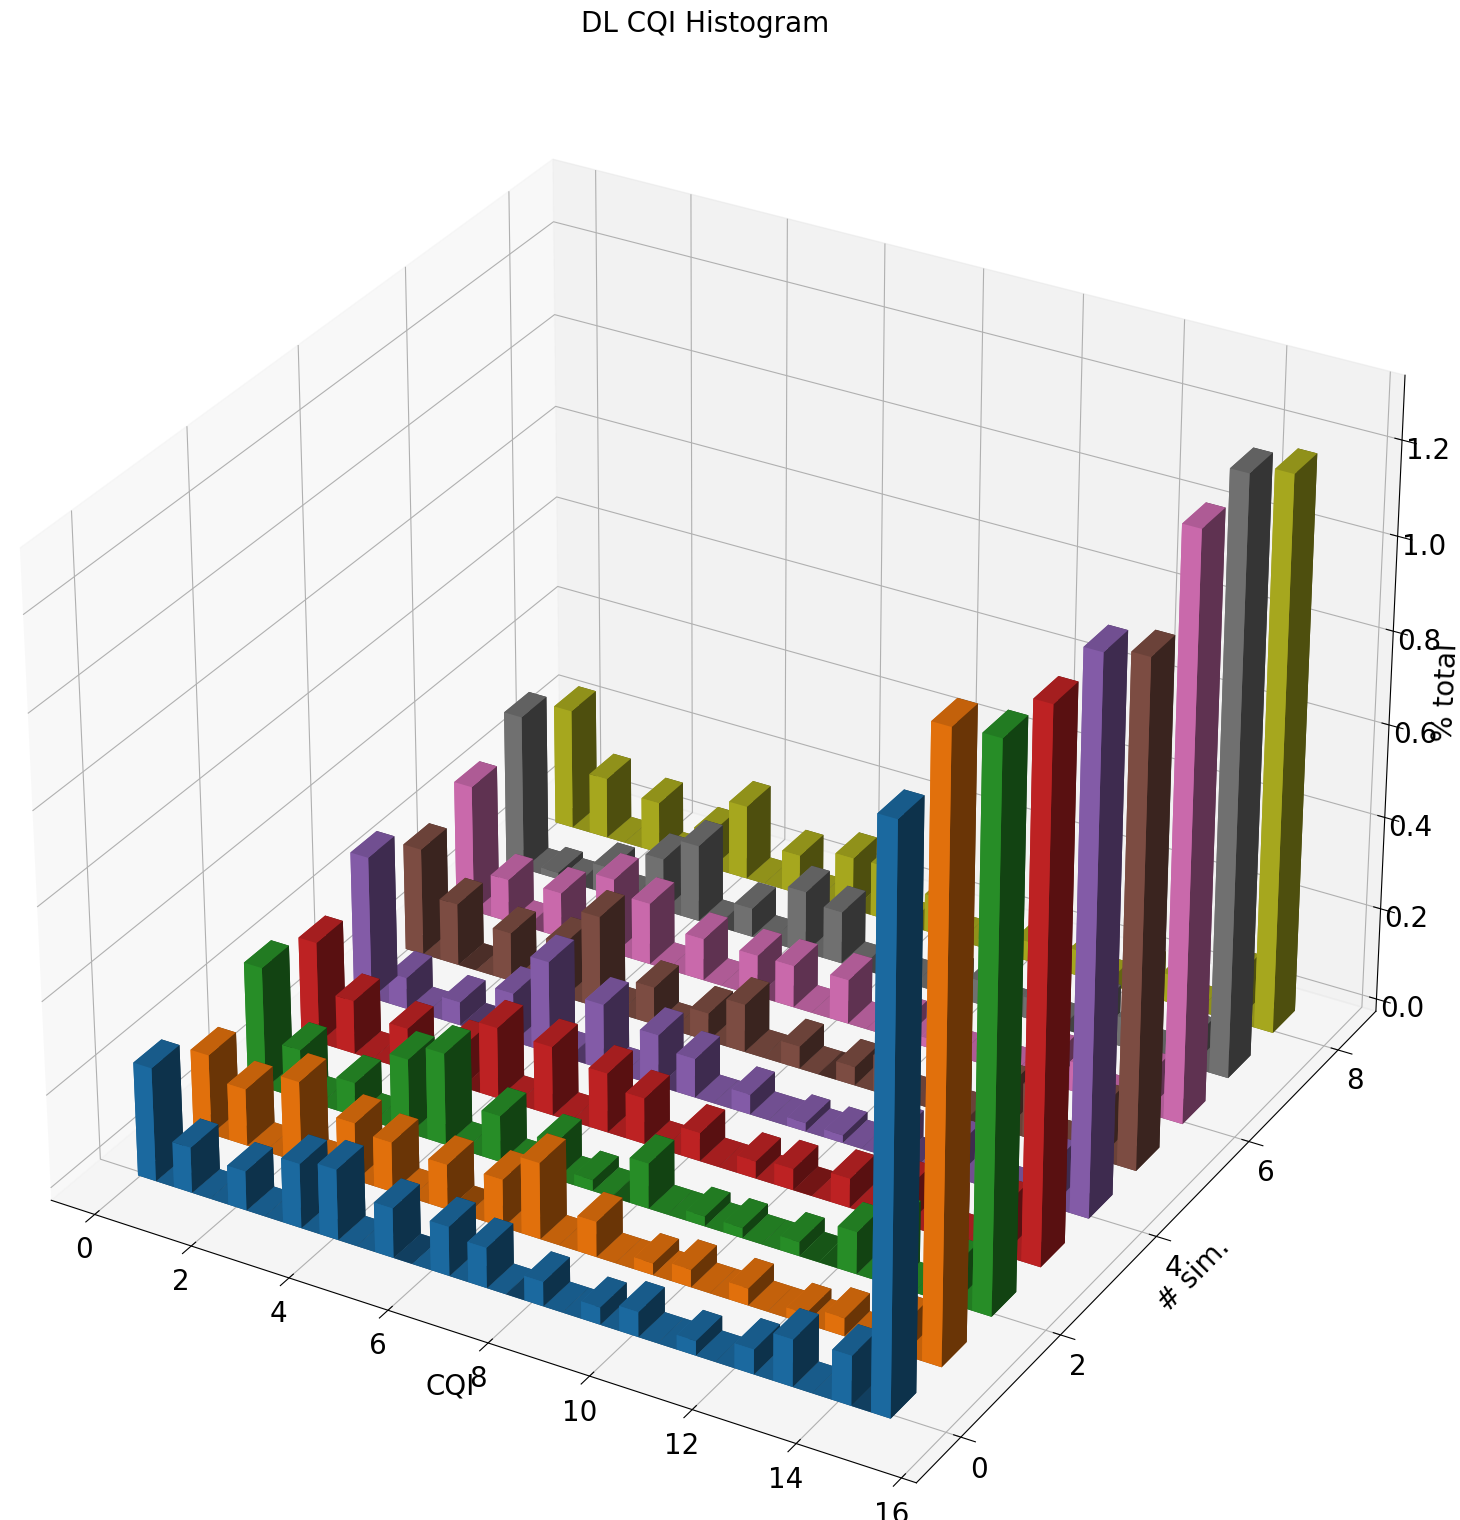
\includegraphics[scale=0.42]{../comparaciones/scheduling_daneses_10mhz_3.5mbps_100ue/ue/cqi_dl_3d_hist_all_ue_multi.png_cropped.png}}
\end{figure}

Si atendemos a los valores indicativos del estado del canal de transmisión (SINR, RSRP, CQI),
podemos ver que éstos no cambian entre métricas (figura 4.21).
Es de esperar, pues el aumento en el número de UE supondrá siempre más interferencia y menos ancho de banda disponible.

\begin{figure}[H]
	\ffigbox[\FBwidth] {
	\caption[Planificación de paquetes - Tercer caso - MCS (I)]{Distribución del índice MCS para la dirección DL.

	Las métricas por orden: FIFO, BET, EDF, LWDF, MT, RR, PF, M-LWDF.}
	}
	{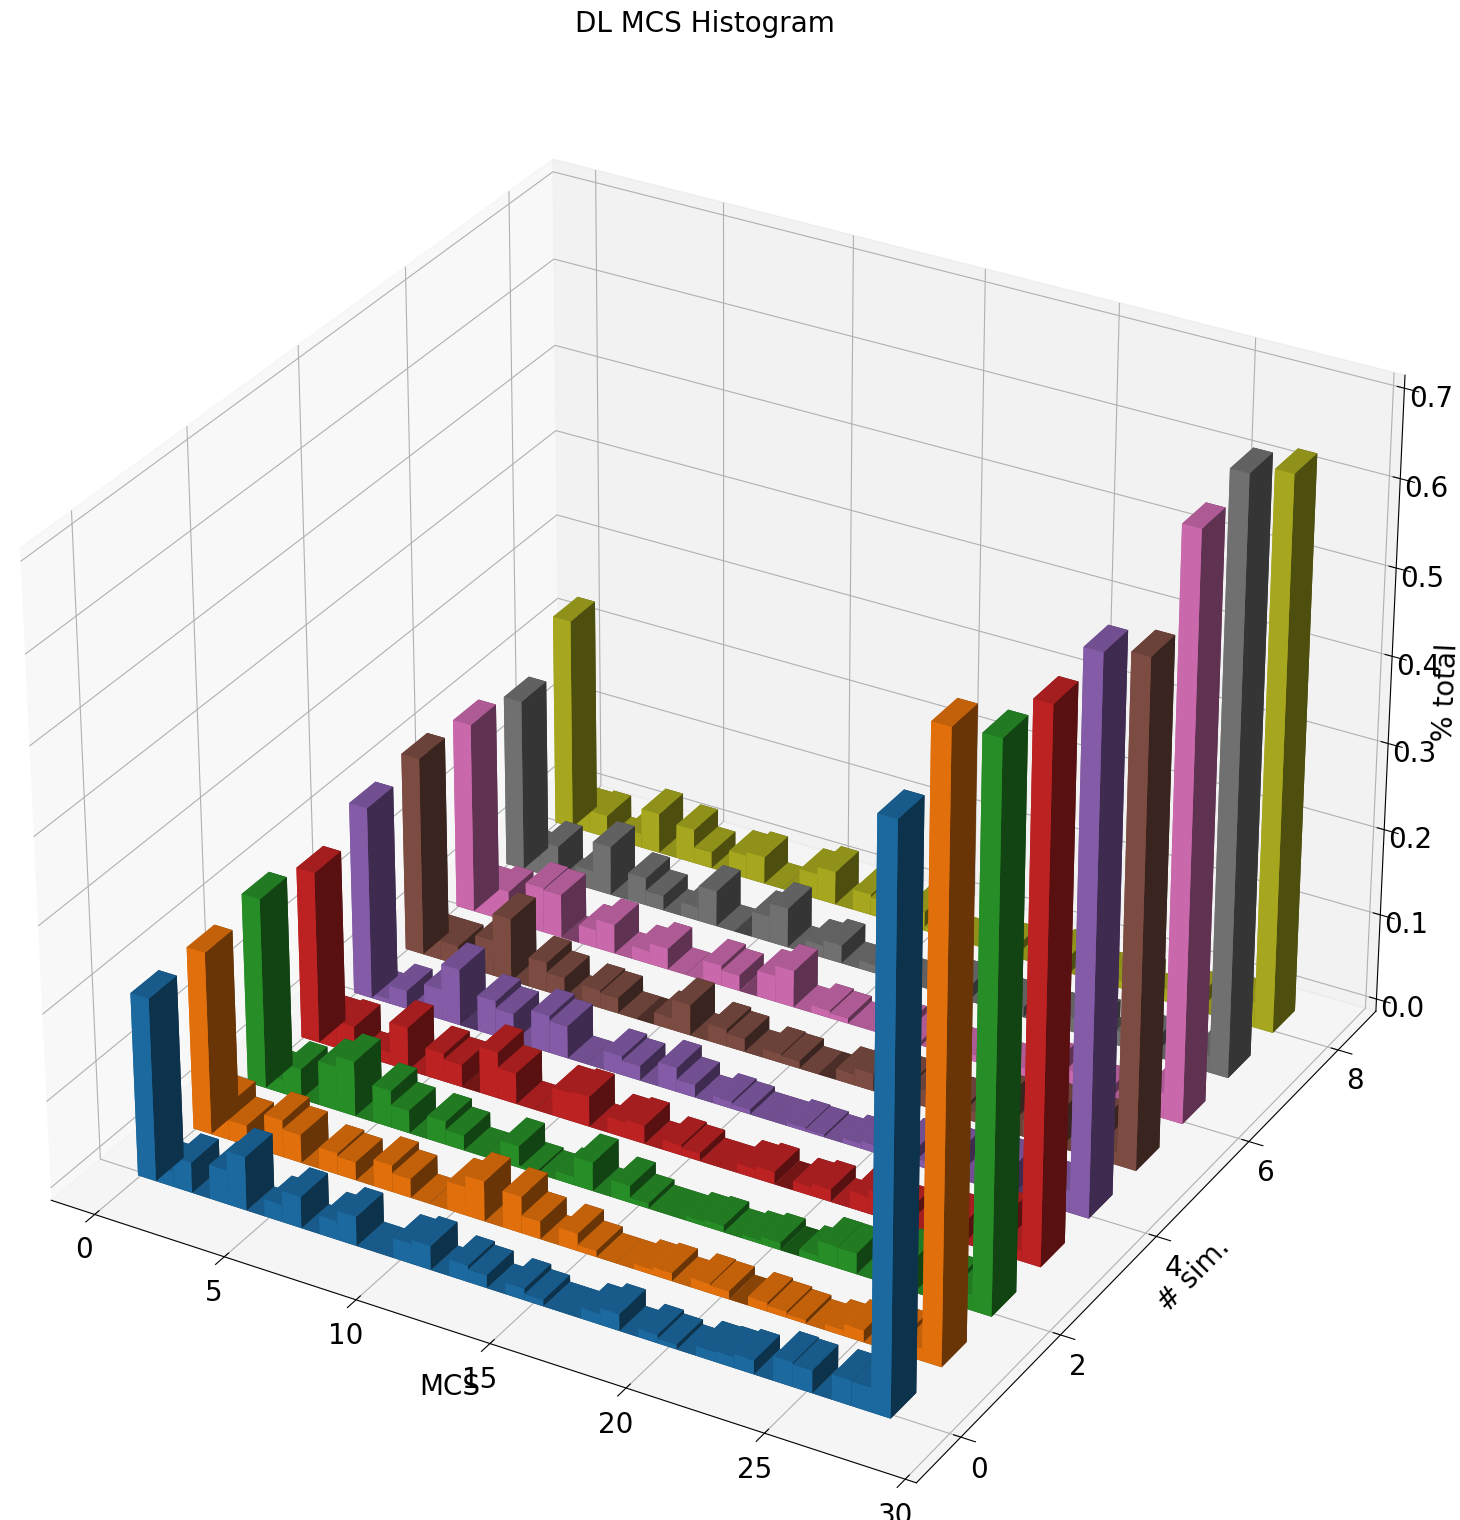
\includegraphics[scale=0.42]{../comparaciones/scheduling_daneses_10mhz_3.5mbps_100ue/ue/mcs_dl_3d_hist_all_ue_multi.png_cropped.png}}
\end{figure}

En la figura 4.22 se puede ver que,
de manera paralela, el índice MCS no cambia entre métricas, sólo entre número de UE en la celda. Además, se concentra en 27 y 0:
Este resultado es, igualmente, esperable, pues los valores SINR, CQI, etc. son los que determinan el valor MCS elegido.
Además, se trata de una celda pequeña, por lo que estos valores son muy parecidos, lo que ocasiona que se concentren en el valor de 27 y 0.

\subsubsection{Latencia y URLLC}

Para el servicio de URLLC, el indicador de prestaciones (\textit{key performance indicator}, KPI) tiene que ver con la latencia;
se trata trata de la latencia más grande detectada para una umbral de fiabilidad elegido, por ejemplo, 99.99 \%.
Por otro lado, la capacidad URLLC de la red será la máxima carga (tasa binaria) que se puede cursar para un umbral de fiabilidad y una latencia máxima elegidos.
\cite{RefWorks:66}

\begin{center}{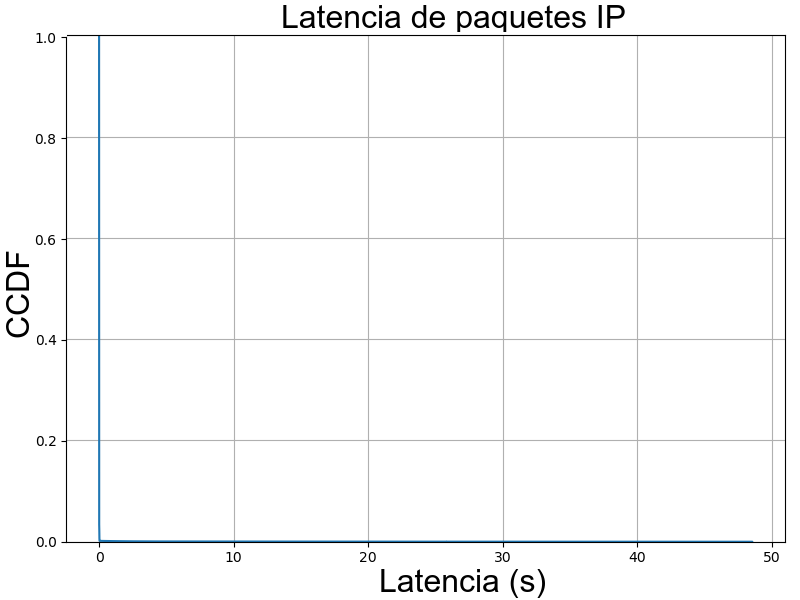
\includegraphics[scale=0.475]{../computos_y_graficas/scheduling_daneses_10mhz_3.5mbps_100ue/5_8_0_38_19/ue/ccdf_ildl.png_fixed.png}}\end{center}

\begin{center}{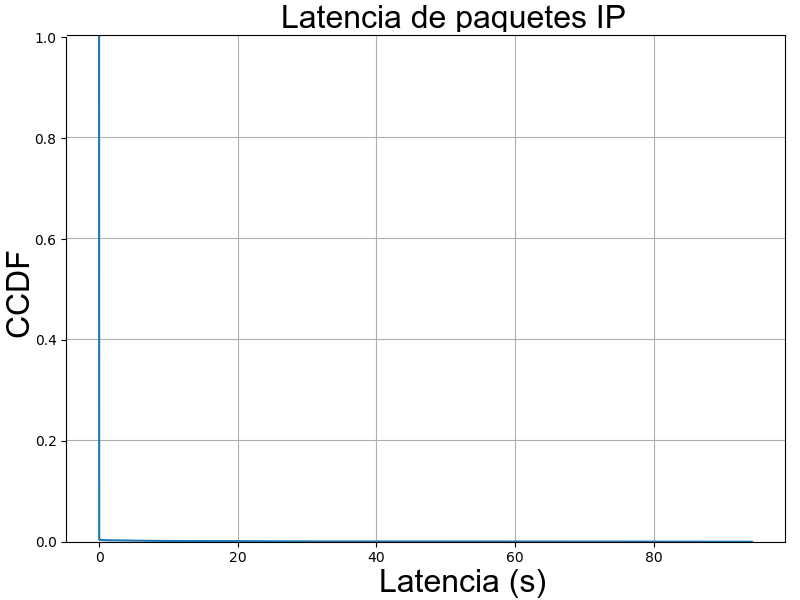
\includegraphics[scale=0.475]{../computos_y_graficas/scheduling_daneses_10mhz_3.5mbps_100ue/5_8_0_40_2/ue/ccdf_ildl.png_fixed.png}}\end{center}

\begin{center}{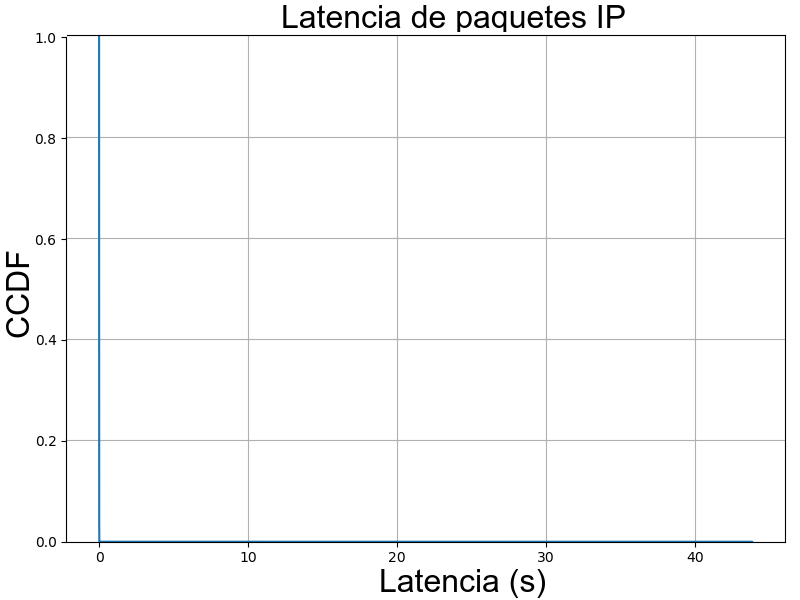
\includegraphics[scale=0.475]{../computos_y_graficas/scheduling_daneses_10mhz_3.5mbps_100ue/5_8_0_41_45/ue/ccdf_ildl.png_fixed.png}}\end{center}

\begin{center}{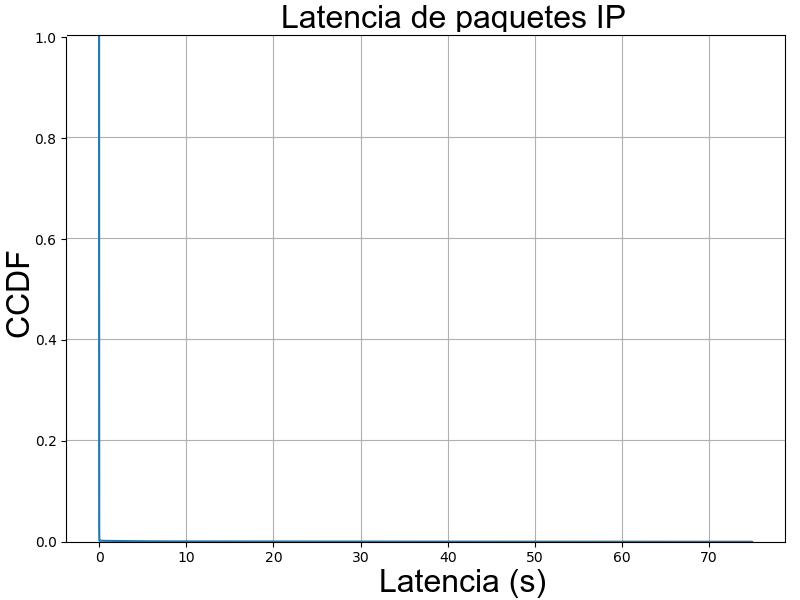
\includegraphics[scale=0.475]{../computos_y_graficas/scheduling_daneses_10mhz_3.5mbps_100ue/5_8_0_43_29/ue/ccdf_ildl.png_fixed.png}}\end{center}

\begin{center}{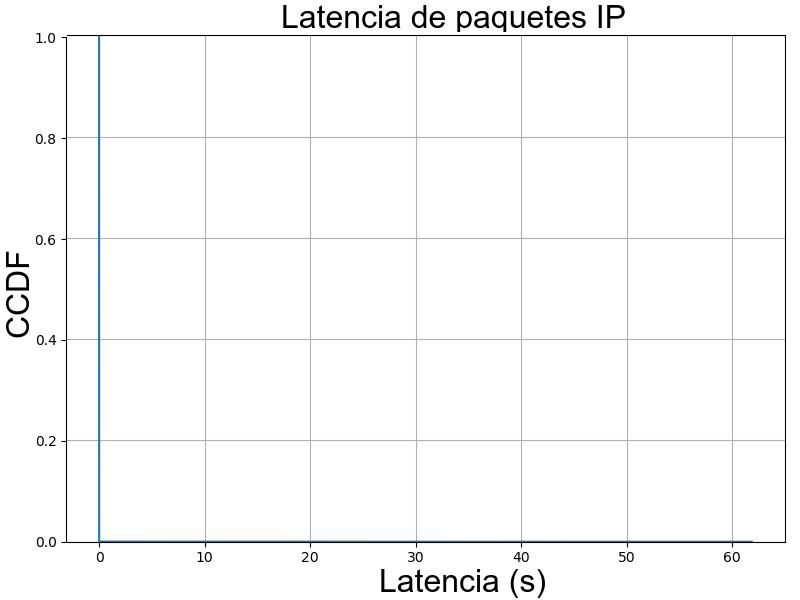
\includegraphics[scale=0.475]{../computos_y_graficas/scheduling_daneses_10mhz_3.5mbps_100ue/5_8_0_45_12/ue/ccdf_ildl.png_fixed.png}}\end{center}

\begin{center}{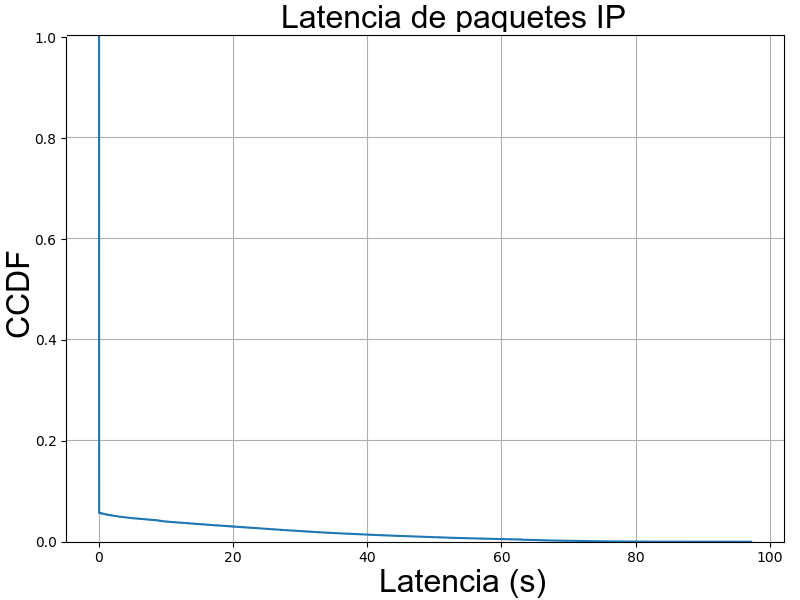
\includegraphics[scale=0.475]{../computos_y_graficas/scheduling_daneses_10mhz_3.5mbps_100ue/5_8_0_46_56/ue/ccdf_ildl.png_fixed.png}}\end{center}

\begin{center}{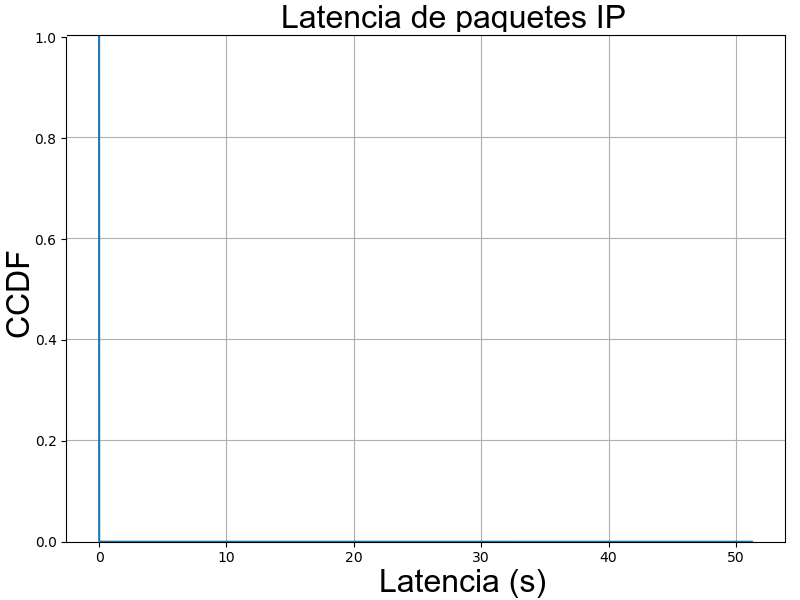
\includegraphics[scale=0.475]{../computos_y_graficas/scheduling_daneses_10mhz_3.5mbps_100ue/5_8_0_48_39/ue/ccdf_ildl.png_fixed.png}}\end{center}

\begin{figure}[H]
	\ffigbox[\FBwidth] {
	\caption[Planificación de paquetes - Tercer caso - Latencia (I)]{CCDF de la latencia de los paquetes IP distintas métricas
	(simulación con 100 UE).

	(Fila 1): FIFO.

	(Fila 2): BET.

	(Fila 3): EDF.

	(Fila 4): LWDF.

	(Fila 5): MT.

	(Fila 6): RR.

	(Fila 7): PF.

	(Fila 8): M-LWDF.}
	}
	{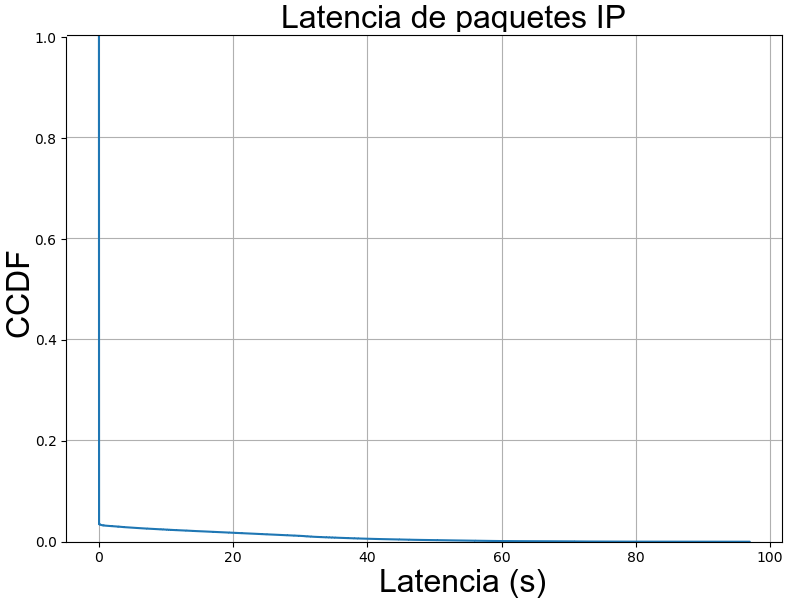
\includegraphics[scale=0.475]{../computos_y_graficas/scheduling_daneses_10mhz_3.5mbps_100ue/5_8_0_50_23/ue/ccdf_ildl.png_fixed.png}}
\end{figure}

Estudiamos la latencia del experimento mediante la función complementaria de la distribución acumulada (\textit{complementary cumulative distribution function}, CCDF) de la latencia.
En primer lugar vemos los resultados del experimento con \textit{FikoRE} en la figura 4.23.
%Por el contrario, las métricas con QoS (M-LWDF) garantiza la entrega del paquete en un tiempo razonable (0.1 s),
En este experimento, M-LWDF ha mostrado peor rendimiento que el esperado;
esto puede atribuirse a una mala configuración de los parámetros que contiene esta métrica \cite{RefWorks:26},
pues está diseñada para descartar los paquetes que excenden el tiempo límite,
pero sin la configuración apropiada, ese límite no se ajusta a los requerimientos de URLLC.
Por lo mismo, algunas métricas sin QoS (FIFO, BET, EDF, LWDF, MT, PF) han logrado mejores prestaciones de latencia que M-LWDF:
su funcionamiento es mejor que una mala configuración de M-LWDF.

Como se concluyó en el apartado anterior y en \cite{RefWorks:26},
la métrica RR, en particular, y las métricas que no están diseñadas con criterios de QoS (MT, LWDF, FIFO, EDF, BET, PF), en general, dan lugar a latencias grandes;
las métricas sin QoS no se pueden usar para servicios que requieran poca latencia.

\begin{center}{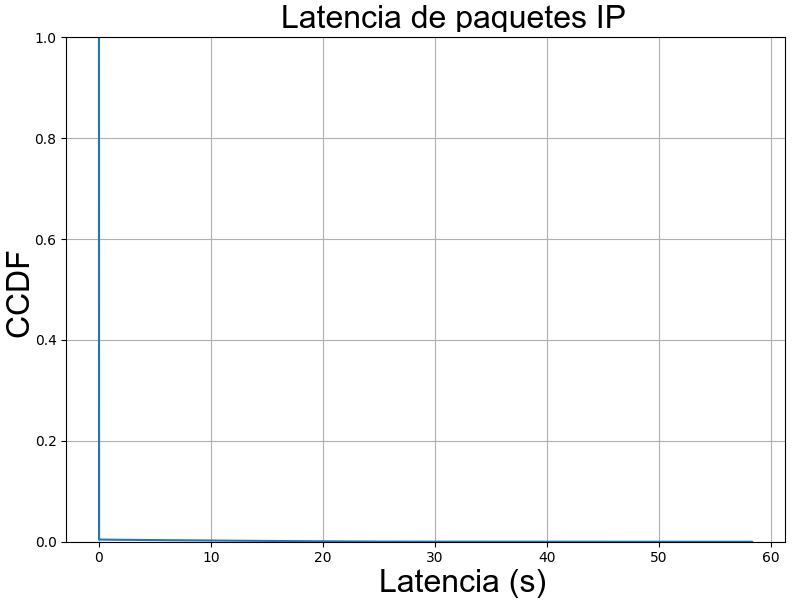
\includegraphics[scale=0.475]{../computos_y_graficas/scheduling_daneses_10mhz_3.5mbps_200ue/5_8_1_4_32/ue/ccdf_ildl.png_fixed.png}}\end{center}

\begin{center}{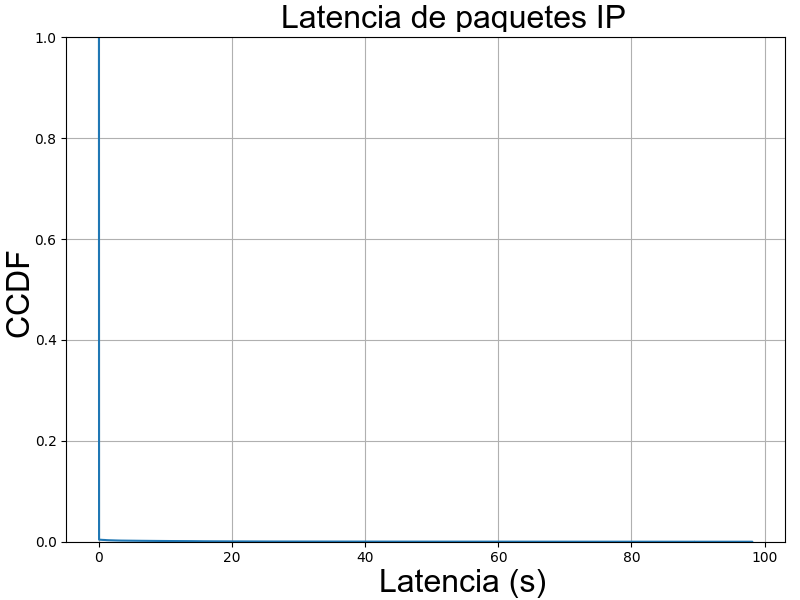
\includegraphics[scale=0.475]{../computos_y_graficas/scheduling_daneses_10mhz_3.5mbps_200ue/5_8_1_6_18/ue/ccdf_ildl.png_fixed.png}}\end{center}

\begin{center}{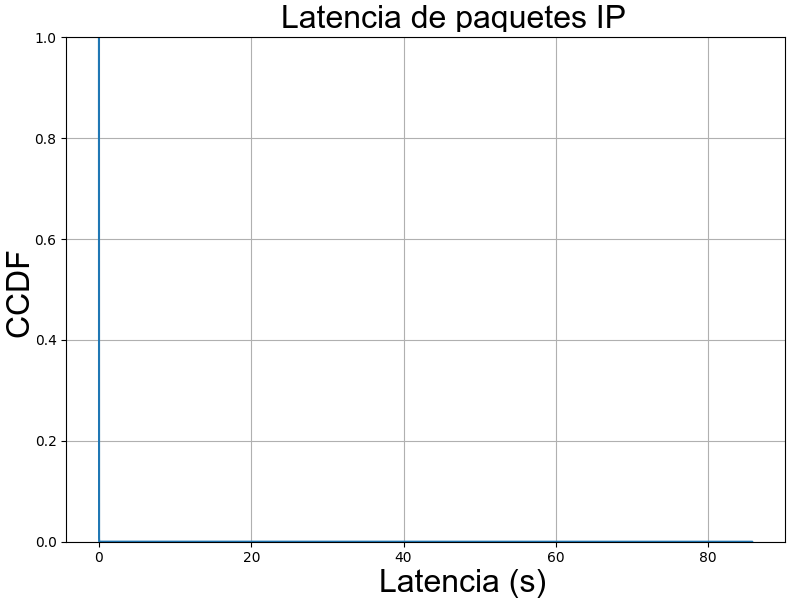
\includegraphics[scale=0.475]{../computos_y_graficas/scheduling_daneses_10mhz_3.5mbps_200ue/5_8_1_8_5/ue/ccdf_ildl.png_fixed.png}}\end{center}

\begin{center}{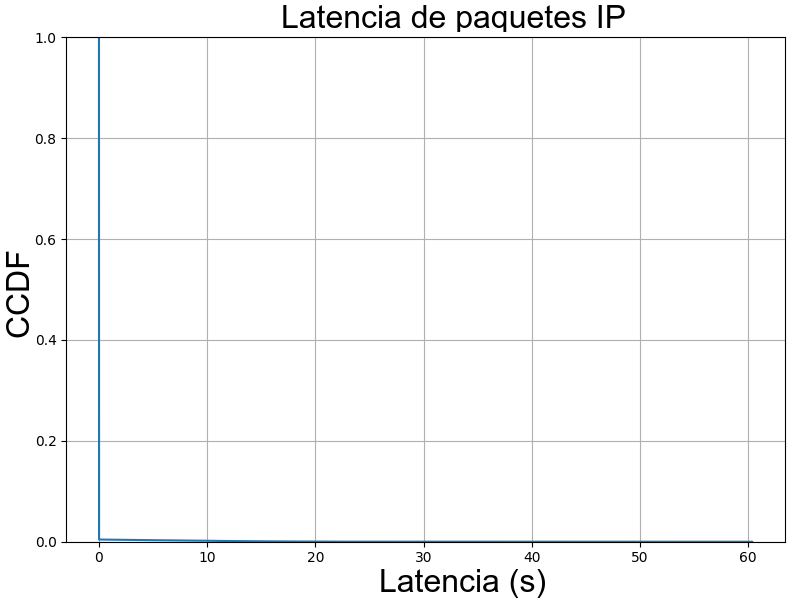
\includegraphics[scale=0.475]{../computos_y_graficas/scheduling_daneses_10mhz_3.5mbps_200ue/5_8_1_9_52/ue/ccdf_ildl.png_fixed.png}}\end{center}

\begin{center}{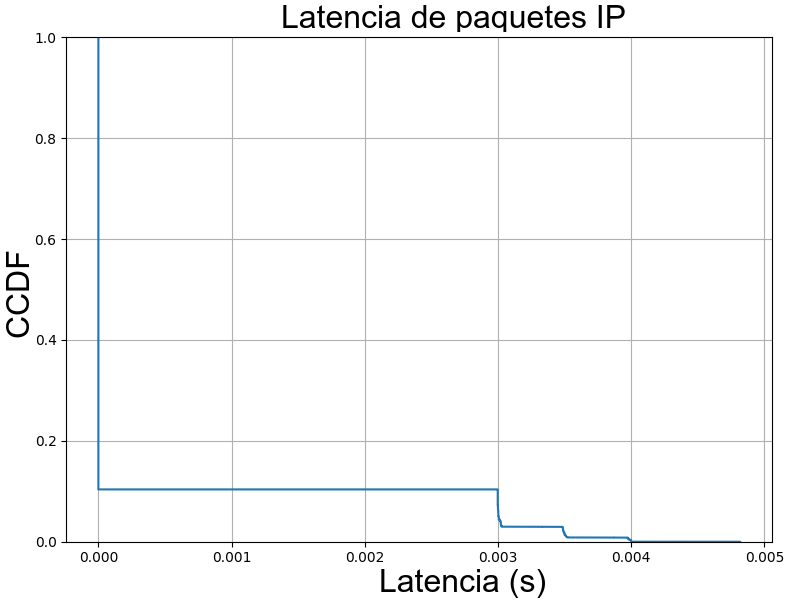
\includegraphics[scale=0.475]{../computos_y_graficas/scheduling_daneses_10mhz_3.5mbps_200ue/5_8_1_11_39/ue/ccdf_ildl.png_fixed.png}}\end{center}

\begin{center}{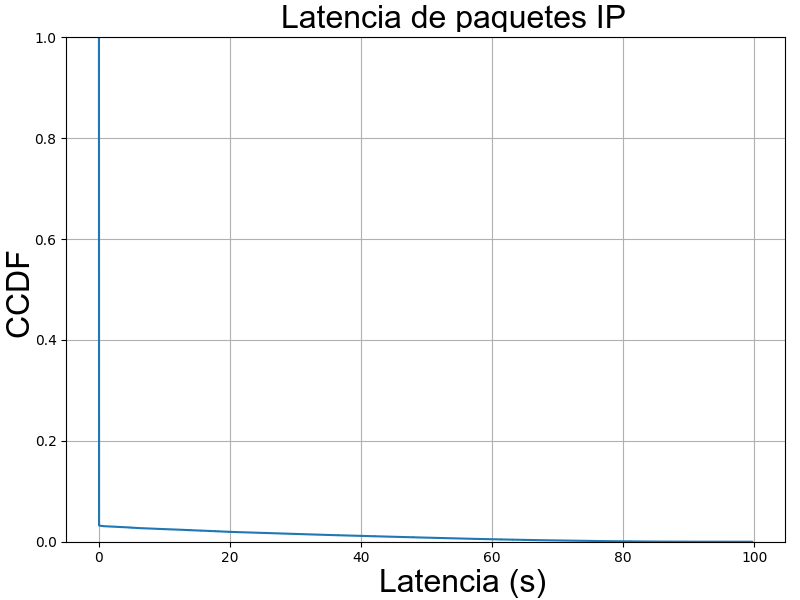
\includegraphics[scale=0.475]{../computos_y_graficas/scheduling_daneses_10mhz_3.5mbps_200ue/5_8_1_13_26/ue/ccdf_ildl.png_fixed.png}}\end{center}

\begin{center}{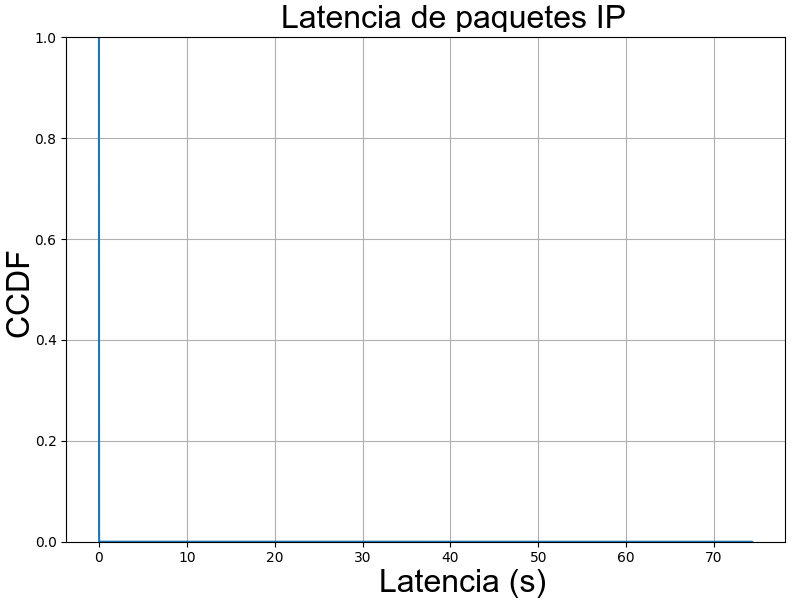
\includegraphics[scale=0.475]{../computos_y_graficas/scheduling_daneses_10mhz_3.5mbps_200ue/5_8_1_15_13/ue/ccdf_ildl.png_fixed.png}}\end{center}

\begin{figure}[H]
	\ffigbox[\FBwidth] {
	\caption[Planificación de paquetes - Tercer caso - Latencia (II)]{CCDF de la latencia de los paquetes IP usando distintas métricas
	(simulación con 200 UE).

	(Fila 1): FIFO.

	(Fila 2): BET.

	(Fila 3): EDF.

	(Fila 4): LWDF.

	(Fila 5): MT.

	(Fila 6): RR.

	(Fila 7): PF.

	(Fila 8): M-LWDF.}
	}
	{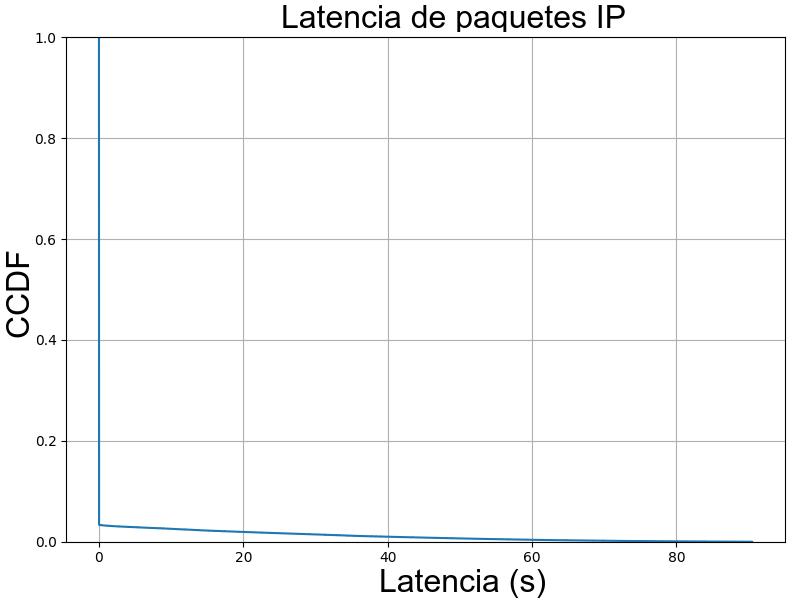
\includegraphics[scale=0.475]{../computos_y_graficas/scheduling_daneses_10mhz_3.5mbps_200ue/5_8_1_17_0/ue/ccdf_ildl.png_fixed.png}}
\end{figure}

En la figura 4.24 podemos ver que,
nuevamente, las métricas que no están diseñadas con criterios de QoS (RR, MT, LWDF, FIFO, EDF, BET, PF) dan lugar a latencias grandes;
en este caso, con mayor afluencia de UE, algunas como MT terminan por demostrar su peor diseño para este cometido.
%Por el contrario, las métricas con QoS (M-LWDF) garantiza la entrega del paquete en un tiempo razonable (0.1 s),
De nuevo, M-LWDF ha mostrado peor rendimiento que el esperado.

%\begin{figure}[H]
%	\ffigbox[\FBwidth] {
%	\caption[Caso - Packet scheduling - Daneses]{CCDF de la latencia de los paquetes IP usando las métricas
%	MT (línea discontinua azul),
%	PF (línea discontinua roja),
%	\textit{TP-Delay} (línea discontinua verde)
%	(experimento de \cite{RefWorks:66}).}
%	}
%	{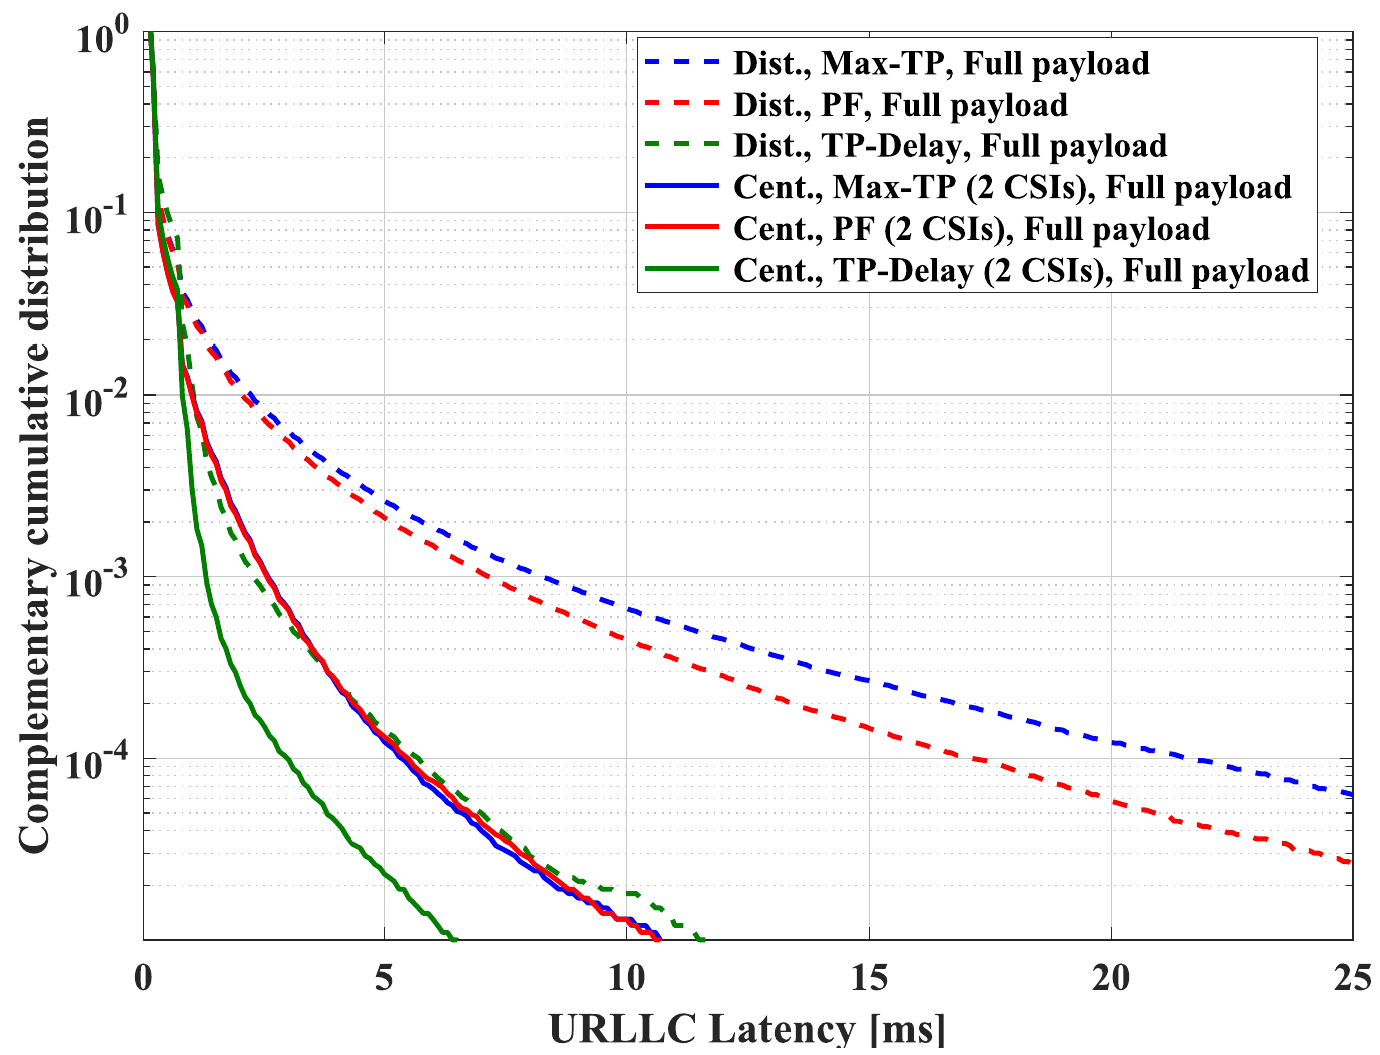
\includegraphics[scale=0.3]{imagenes/scheduling_daneses/scheduling_daneses-003.png}}
%\end{figure}
%
%\begin{figure}[H]
%	\ffigbox[\FBwidth] {
%	\caption[Caso - Packet scheduling - Daneses]{CCDF de la latencia de los paquetes IP usando las métricas
%	PF (línea continua rosa),
%	\textit{TP-Delay} (línea continua azul)
%	(experimento de \cite{RefWorks:66}).}
%	}
%	{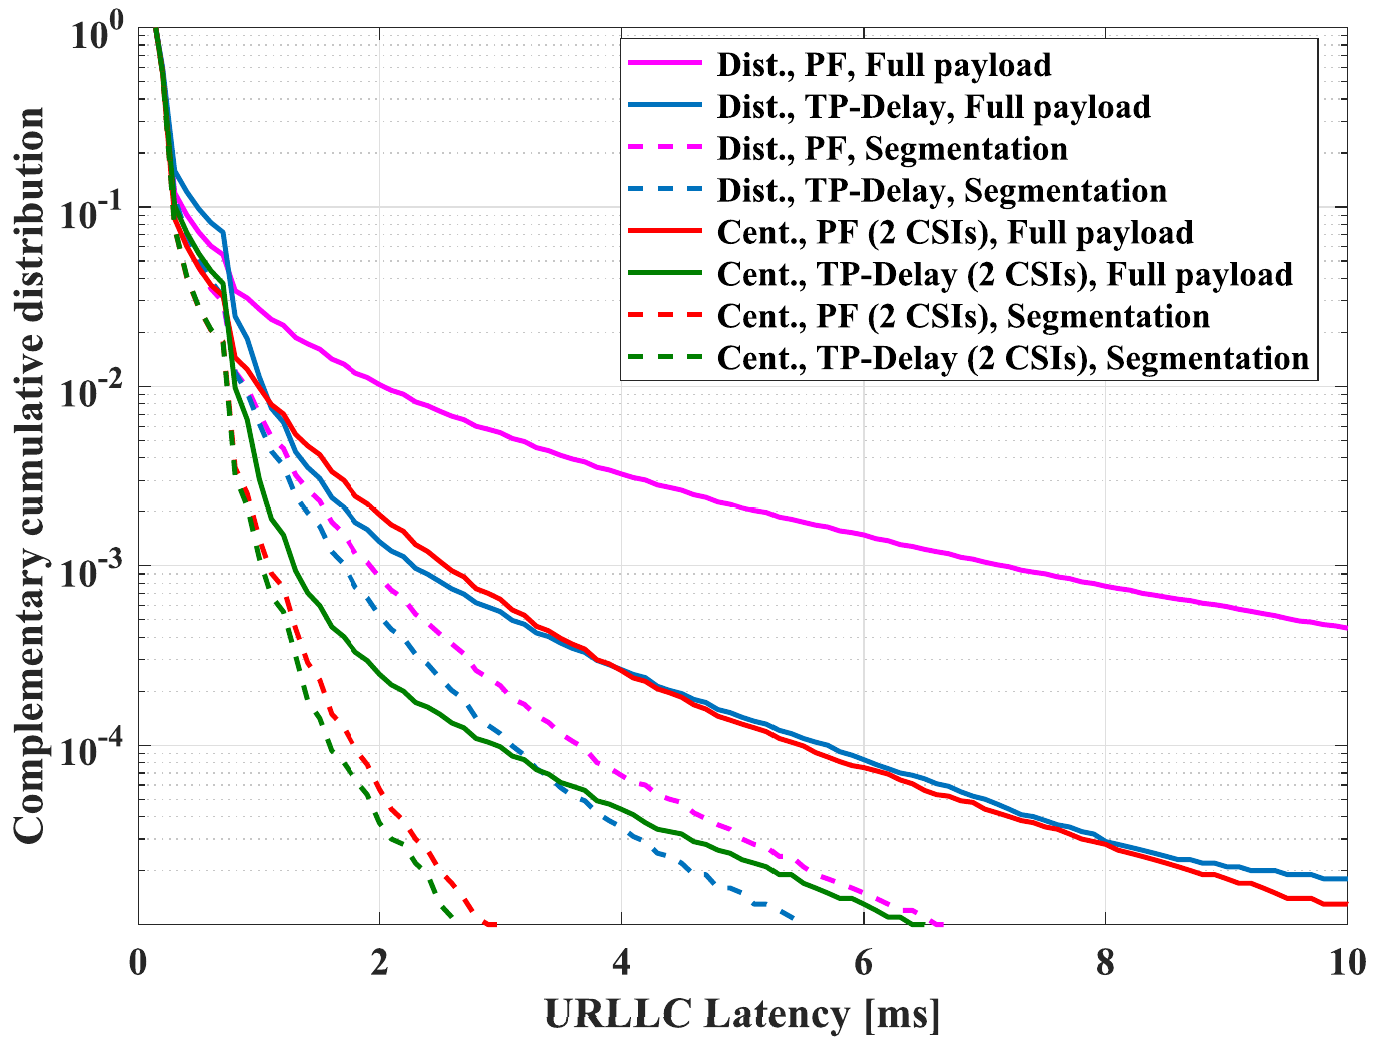
\includegraphics[scale=0.3]{imagenes/scheduling_daneses/scheduling_daneses-005.png}}
%\end{figure}
%
%\begin{figure}[H]
%	\ffigbox[\FBwidth] {
%	\caption[Caso - Packet scheduling - Daneses]{CCDF de la latencia de los paquetes IP usando la métrica
%	\textit{TP-Delay} (línea continua morada)
%	(experimento de \cite{RefWorks:66}).}
%	}
%	{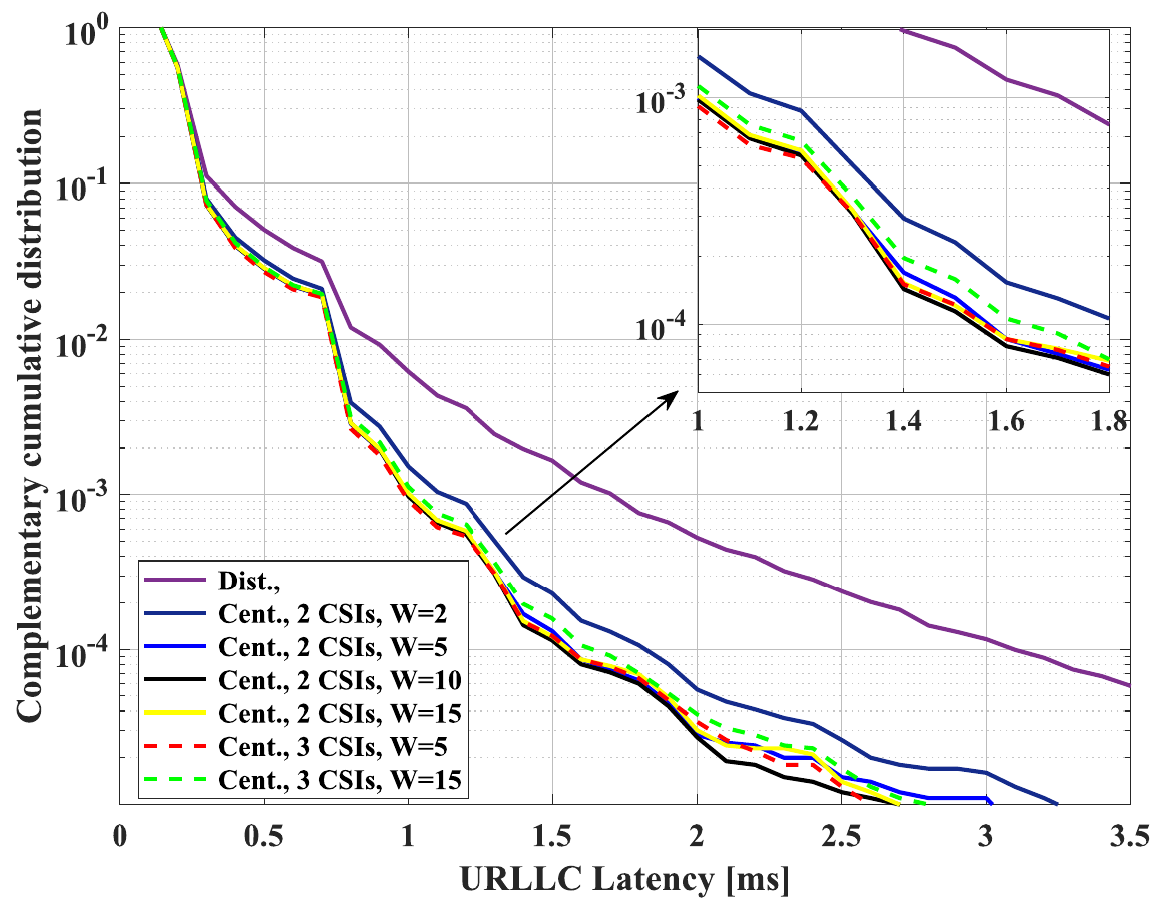
\includegraphics[scale=0.35]{imagenes/scheduling_daneses/scheduling_daneses-009.png}}
%\end{figure}

\begin{center}{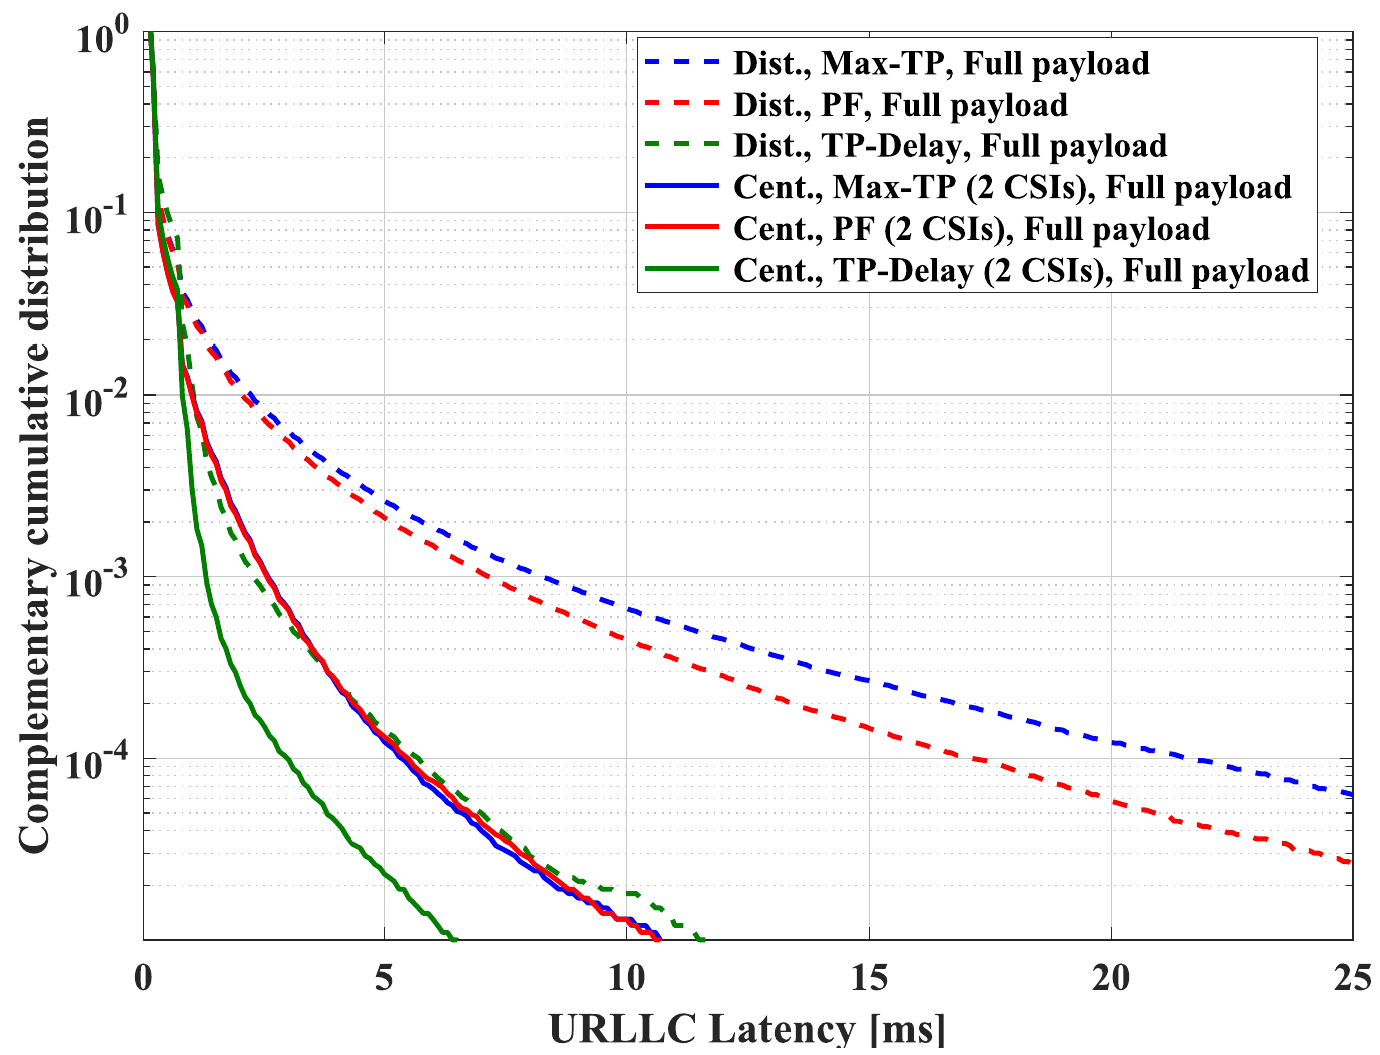
\includegraphics[scale=0.3]{imagenes/scheduling_daneses/scheduling_daneses-003.png}}\end{center}

\begin{center}{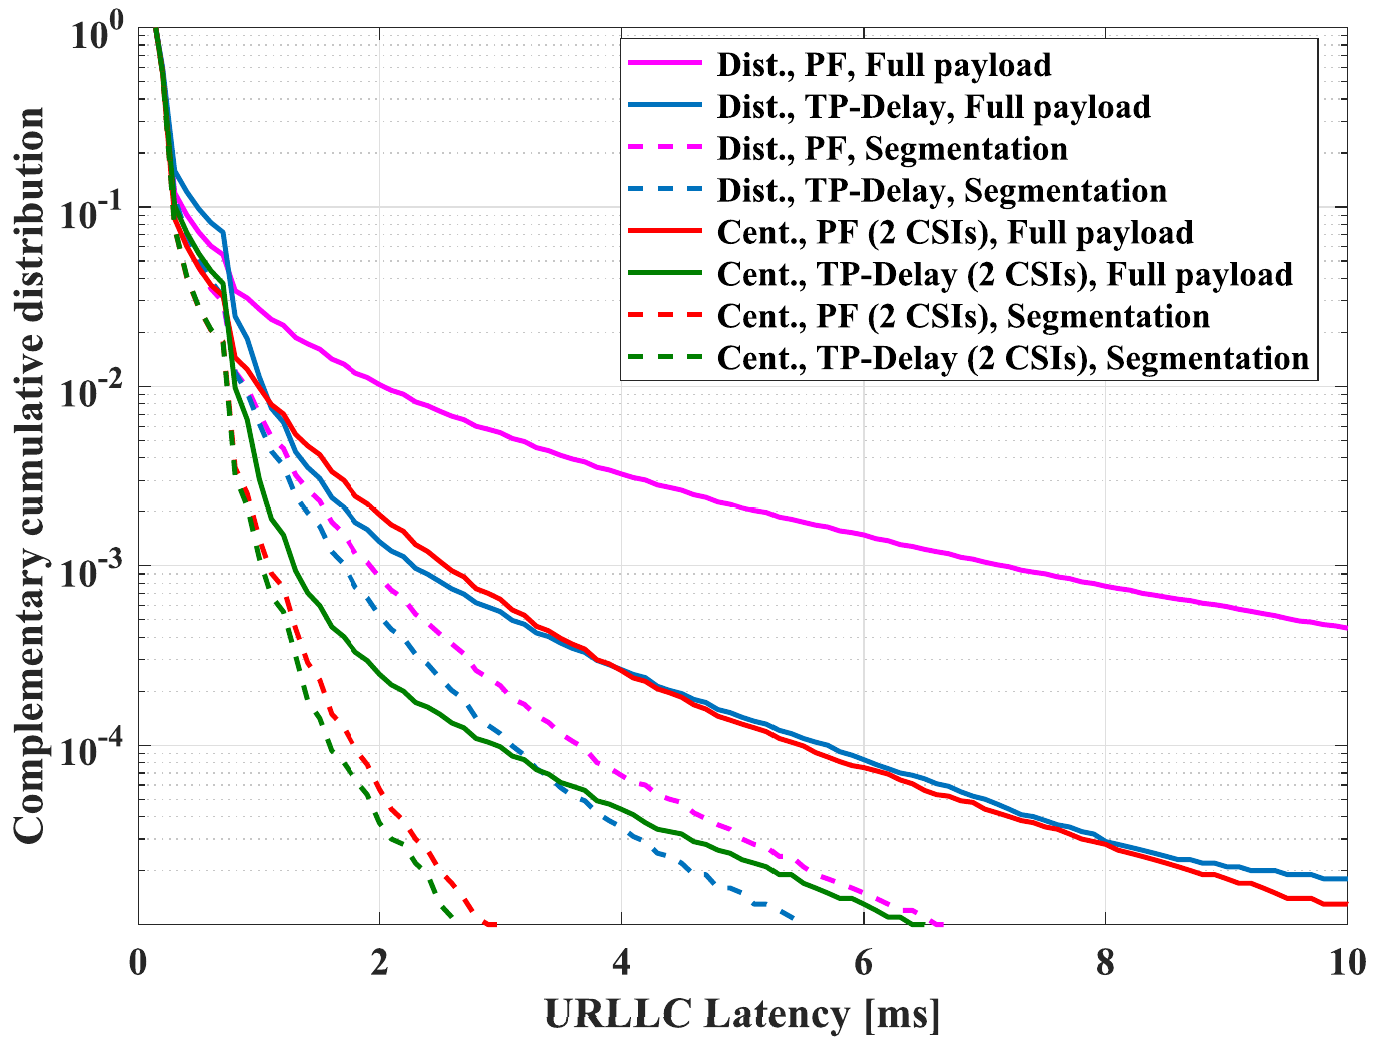
\includegraphics[scale=0.3]{imagenes/scheduling_daneses/scheduling_daneses-005.png}}\end{center}

\begin{figure}[H]
	\ffigbox[\FBwidth] {
	\caption[Planificación de paquetes - Tercer caso - Latencia en el artículo]{CCDF de la latencia de los paquetes IP en el experimento de \cite{RefWorks:66}.

	(Fila 1): Métricas
	MT (línea discontinua azul),
	PF (línea discontinua roja),
	\textit{TP-Delay} (línea discontinua verde).

	(Fila 2): Métricas
	PF (línea continua rosa),
	\textit{TP-Delay} (línea continua azul).

	(Fila 3): Métricas
	\textit{TP-Delay} (línea continua morada).}
	}
	{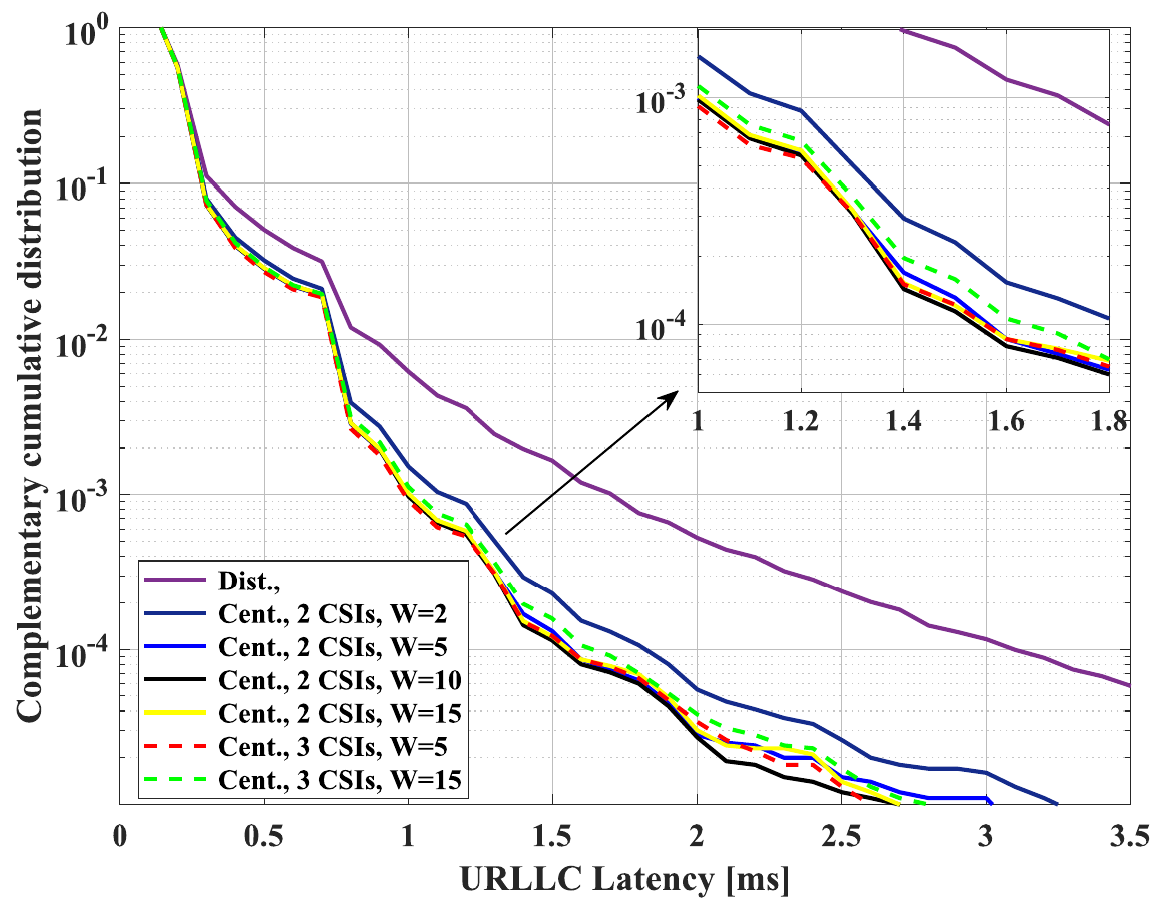
\includegraphics[scale=0.35]{imagenes/scheduling_daneses/scheduling_daneses-009.png}}
\end{figure}

%\begin{figure}[H]
%	\ffigbox[\FBwidth] {
%	\caption[Caso - Packet scheduling - Daneses]{Prestaciones de la red para diferentes presupuestos de latencia y probabilidad de interrupción de de $100 \cdot 10^{-6}$
%	(experimento de \cite{RefWorks:66}).}
%	}
%	{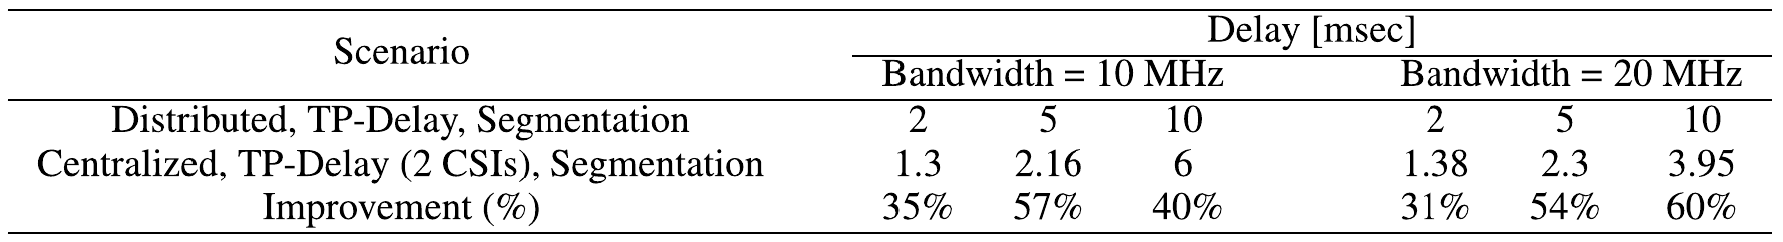
\includegraphics[scale=0.3]{imagenes/scheduling_daneses/scheduling_daneses-006.png}}
%\end{figure}

En la figura 4.25, observamos los experimentos comparables llevados a cabo en \cite{RefWorks:66}.
Se puede observar que, al igual que en nuestro caso, las métricas que no están diseñadas con criterios de QoS (MT, PF) dan lugar a latencias grandes.
El mejor resultado lo da la métrica \textit{TP-Delay}, que se ha diseñado para maximizar tasa binaria y reducir la latencia;
es una métrica que se adecúa al caso de uso de URLLC, que requiere baja latencia y gran fiabilidad.

\subsubsection{Otras prestaciones en URLLC}

Las conclusiones expuestas también se pueden constatar observando otros aspectos de la simulación, especialmente los relativos al comportamiento del sistema en tiempo real.

\begin{center}{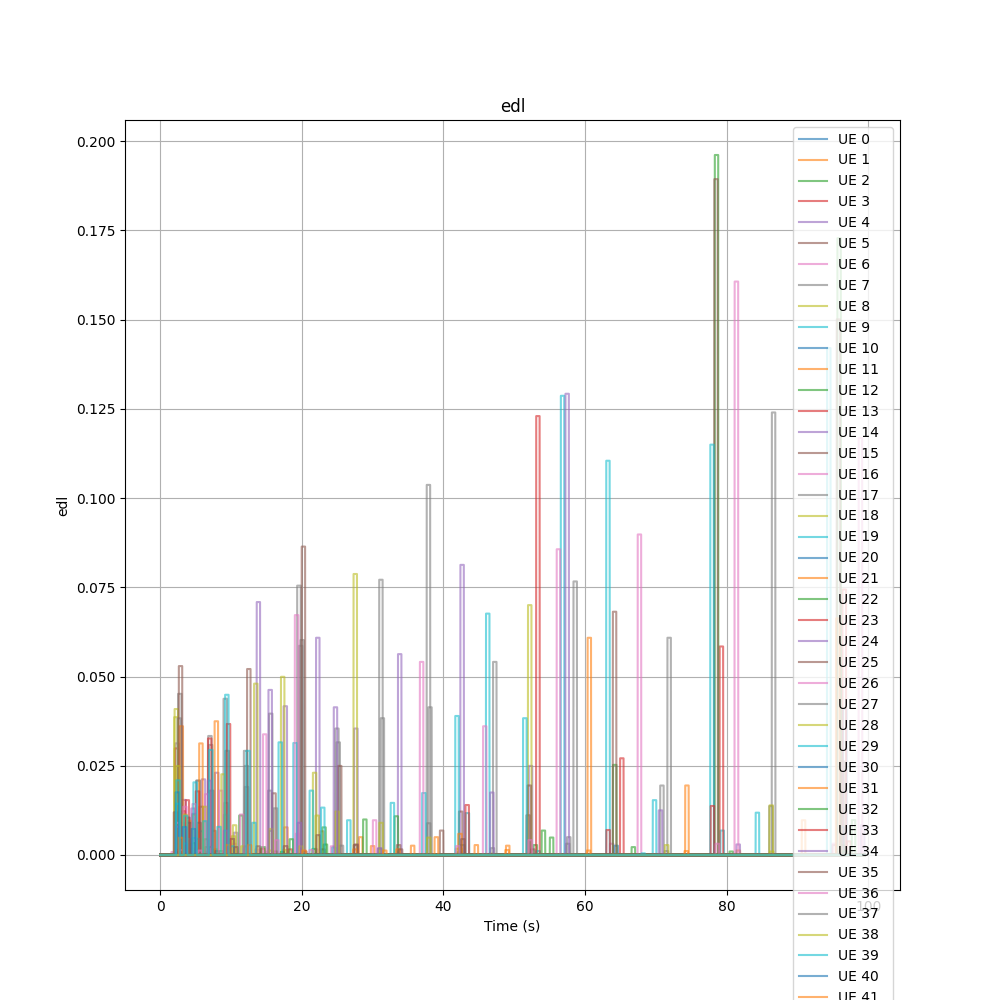
\includegraphics[scale=0.6]{../computos_y_graficas/scheduling_daneses_10mhz_3.5mbps_200ue/5_8_1_4_32/ue/edl_instantaneous.png}}\end{center}

\begin{center}{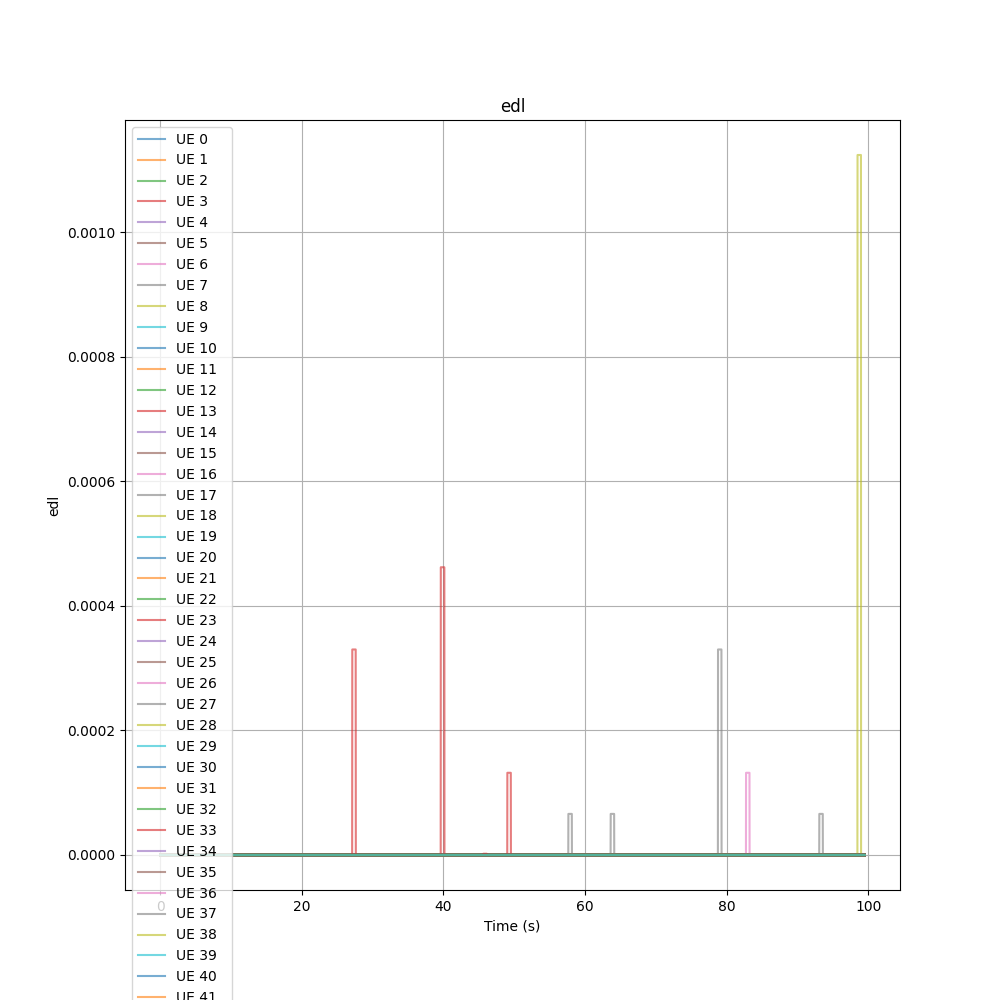
\includegraphics[scale=0.6]{../computos_y_graficas/scheduling_daneses_10mhz_3.5mbps_200ue/5_8_1_6_18/ue/edl_instantaneous.png}}\end{center}

\begin{center}{\includegraphics[scale=0.6]{../computos_y_graficas/scheduling_daneses_10mhz_3.5mbps_200ue/5_8_1_8_5/ue/edl_instantaneous.png}}\end{center}

\begin{center}{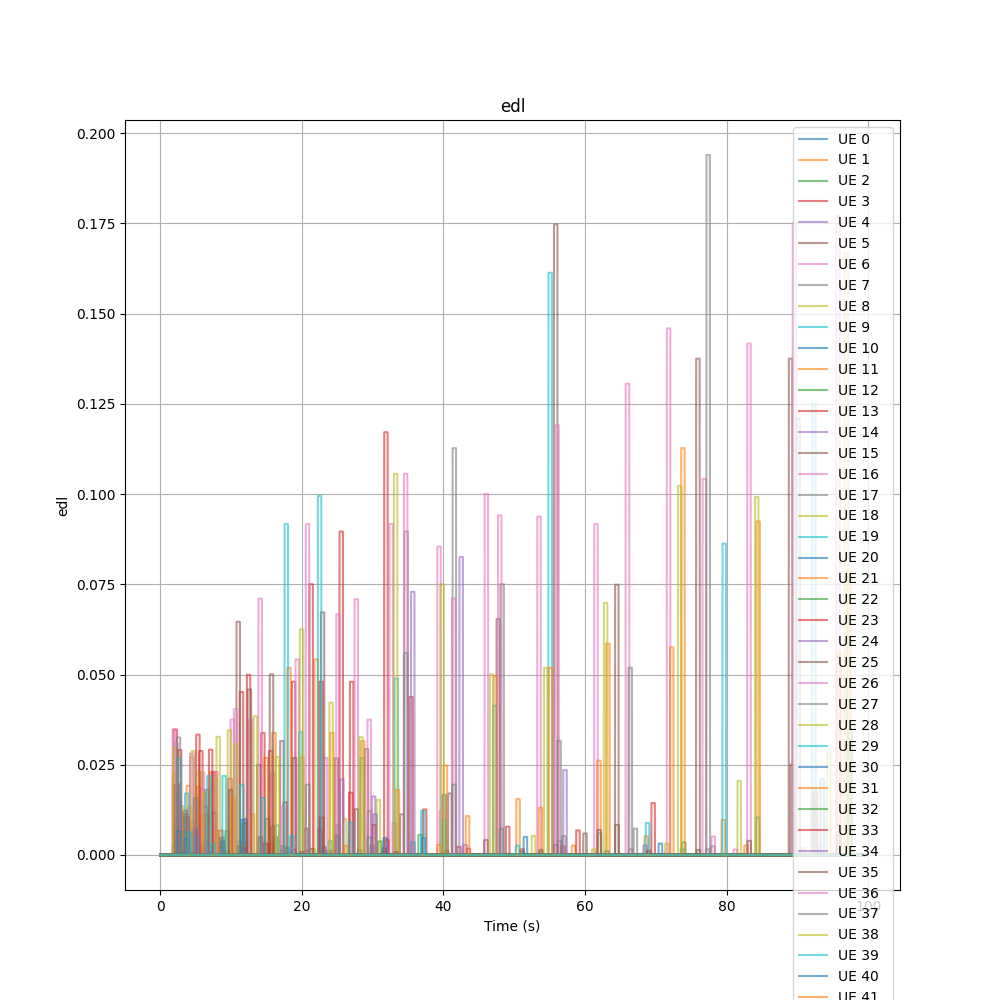
\includegraphics[scale=0.6]{../computos_y_graficas/scheduling_daneses_10mhz_3.5mbps_200ue/5_8_1_9_52/ue/edl_instantaneous.png}}\end{center}

\begin{center}{\includegraphics[scale=0.6]{../computos_y_graficas/scheduling_daneses_10mhz_3.5mbps_200ue/5_8_1_11_39/ue/edl_instantaneous.png}}\end{center}

\begin{center}{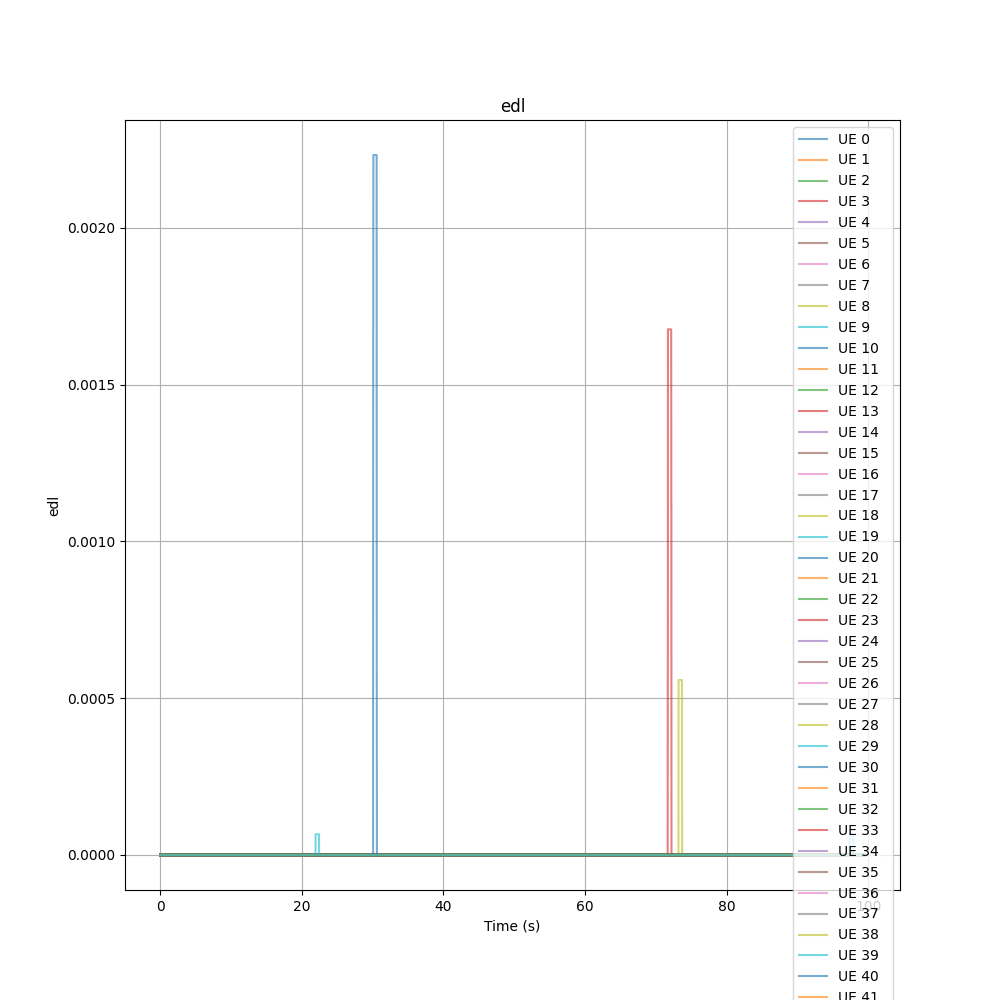
\includegraphics[scale=0.6]{../computos_y_graficas/scheduling_daneses_10mhz_3.5mbps_200ue/5_8_1_13_26/ue/edl_instantaneous.png}}\end{center}

\begin{center}{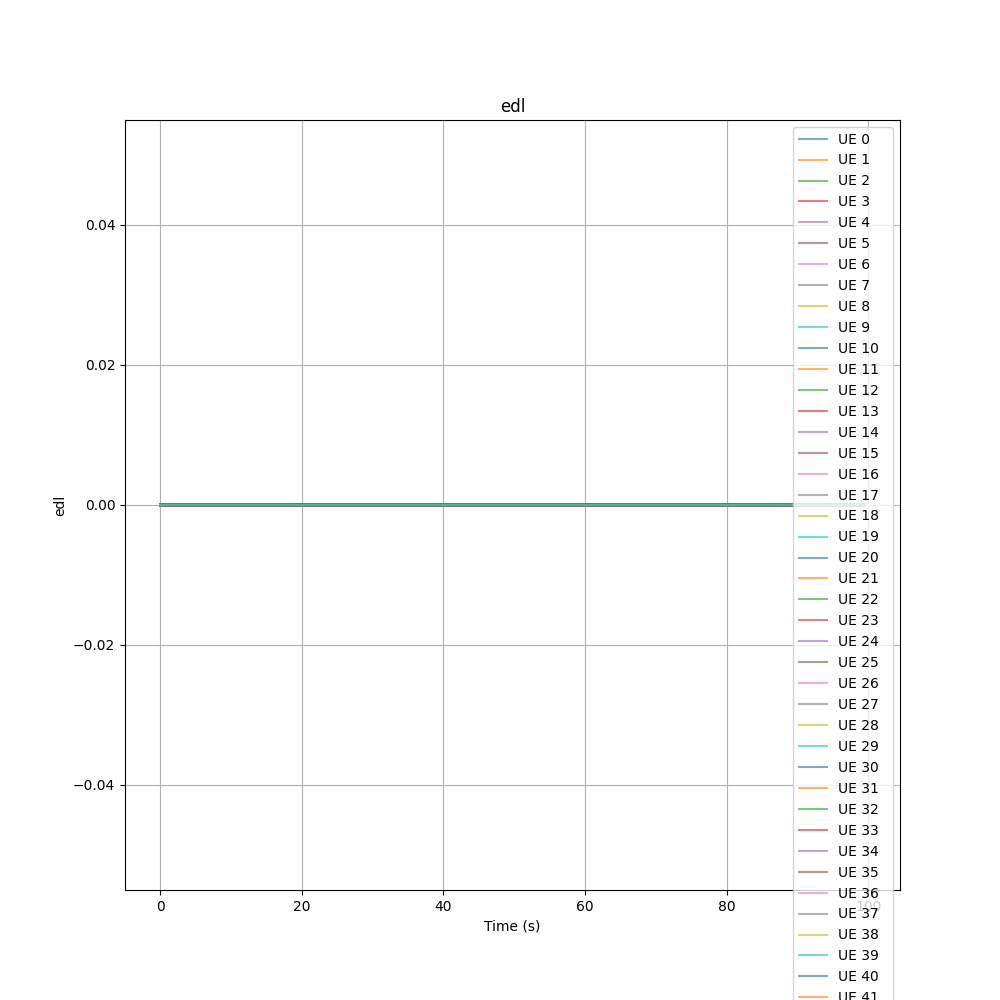
\includegraphics[scale=0.6]{../computos_y_graficas/scheduling_daneses_10mhz_3.5mbps_200ue/5_8_1_15_13/ue/edl_instantaneous.png}}\end{center}

\begin{figure}[H]
	\ffigbox[\FBwidth] {
	\caption[Planificación de paquetes - Tercer caso - Error (I)]{Tasa de error binario en tiempo real en dirección DL usando distintas métricas
	(simulación con 200 UE).

	(Fila 1): FIFO.

	(Fila 2): BET.

	(Fila 3): EDF.

	(Fila 4): LWDF.

	(Fila 5): MT.

	(Fila 6): RR.

	(Fila 7): PF.

	(Fila 8): M-LWDF.}
	}
	{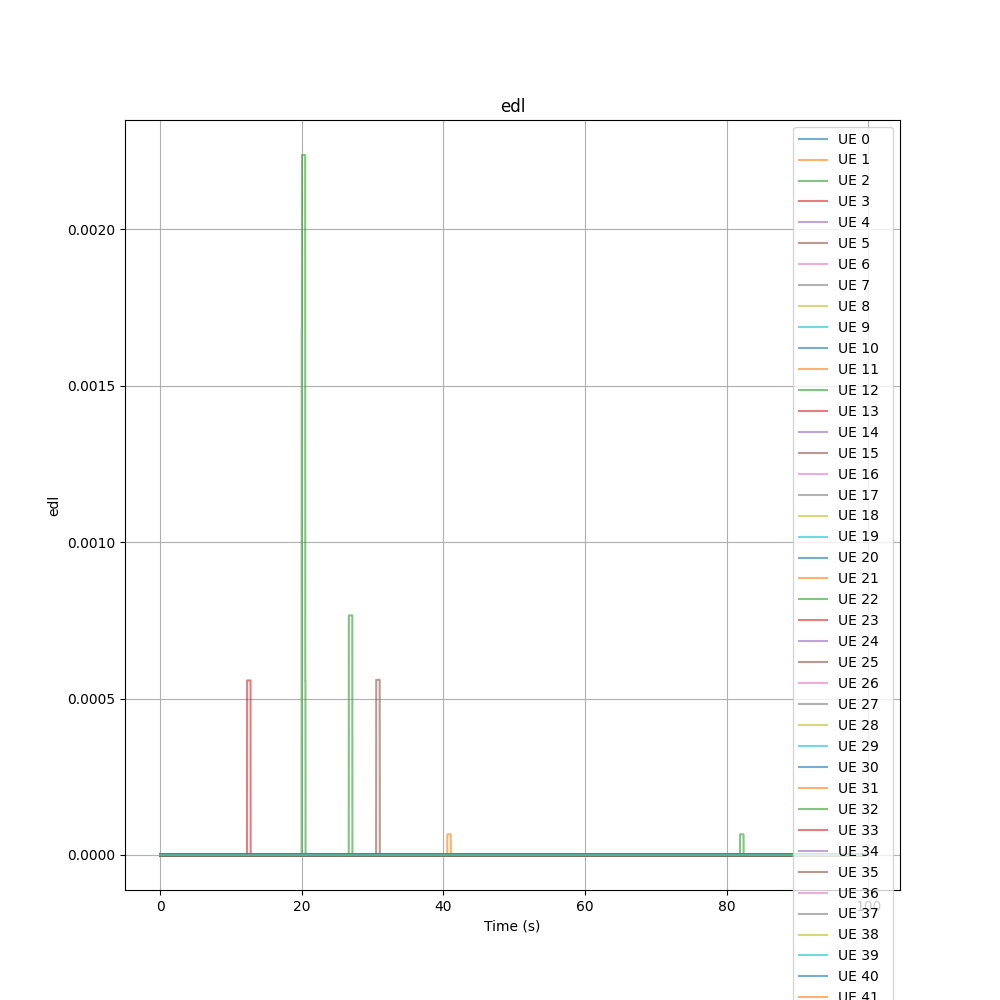
\includegraphics[scale=0.6]{../computos_y_graficas/scheduling_daneses_10mhz_3.5mbps_200ue/5_8_1_17_0/ue/edl_instantaneous.png}}
\end{figure}

En primer lugar observamos la tasa de error binario en la figura 4.26.
Podemos ver que FIFO y LWDF comienzan con tasas de error bajas en todos los UE, que se van estabilizando en valores bajos,
pero sigue habiendo picos repentinos de errores de UE que algún UE que no ha podido transmitir;
FIFO atiende al primer UE en solicitarlo, no está diseñado con criterios de QoS, por lo que al principio quedan muchos fuera,
mientras que LWDF sí está diseñado para prevenir la expiración de un tiempo límite,
lo que puede ocasionar que tarde unos segundos en estabilizarse la asignación.
BET, RR y M-LWDF tienen solo errores en casos raros y EDF, MT y PF no tienen errores;
M-LWDF sí está diseñada con criterios de QoS, por lo que evita que se pierdan paquetes,
mientras que el resto de métricas, quizás por ser más sencillas, asignaban pronto recursos de radio y prevenían que el error se incrementase.

\begin{center}{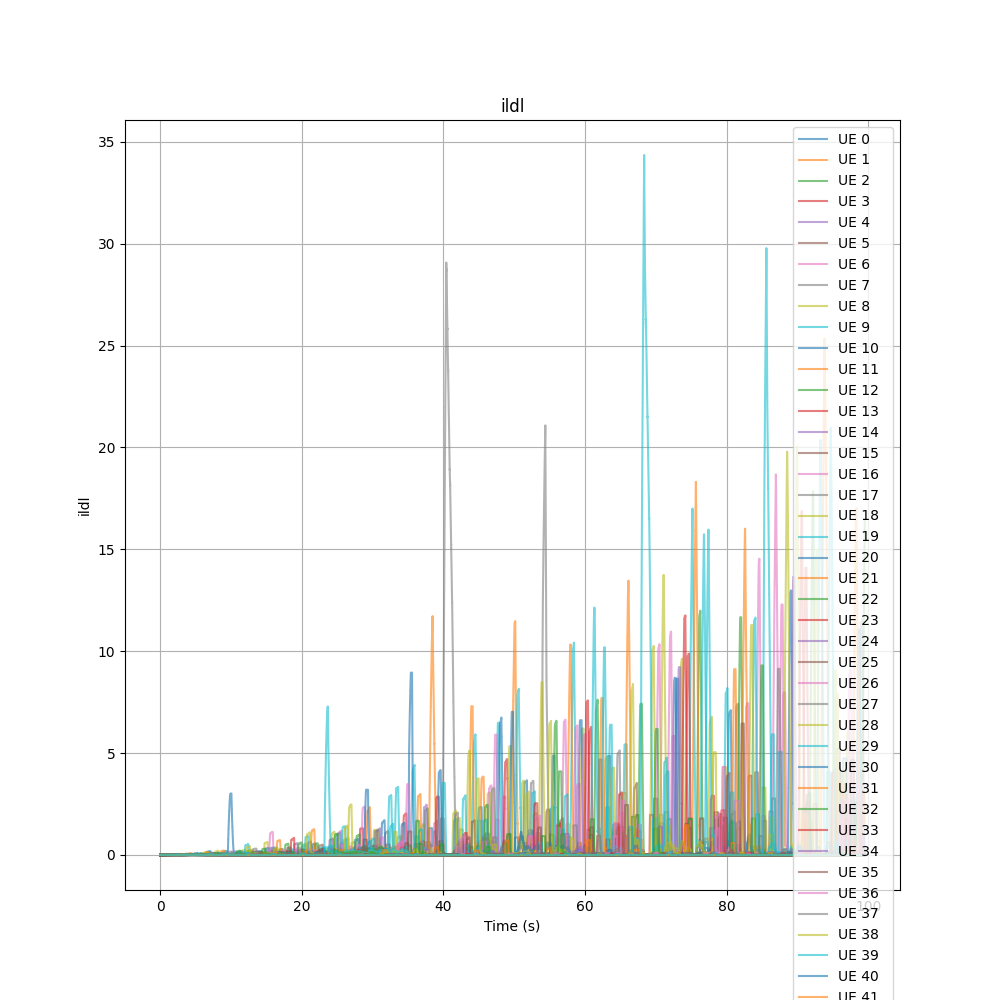
\includegraphics[scale=0.6]{../computos_y_graficas/scheduling_daneses_10mhz_3.5mbps_200ue/5_8_1_4_32/ue/ildl_instantaneous.png}}\end{center}

\begin{center}{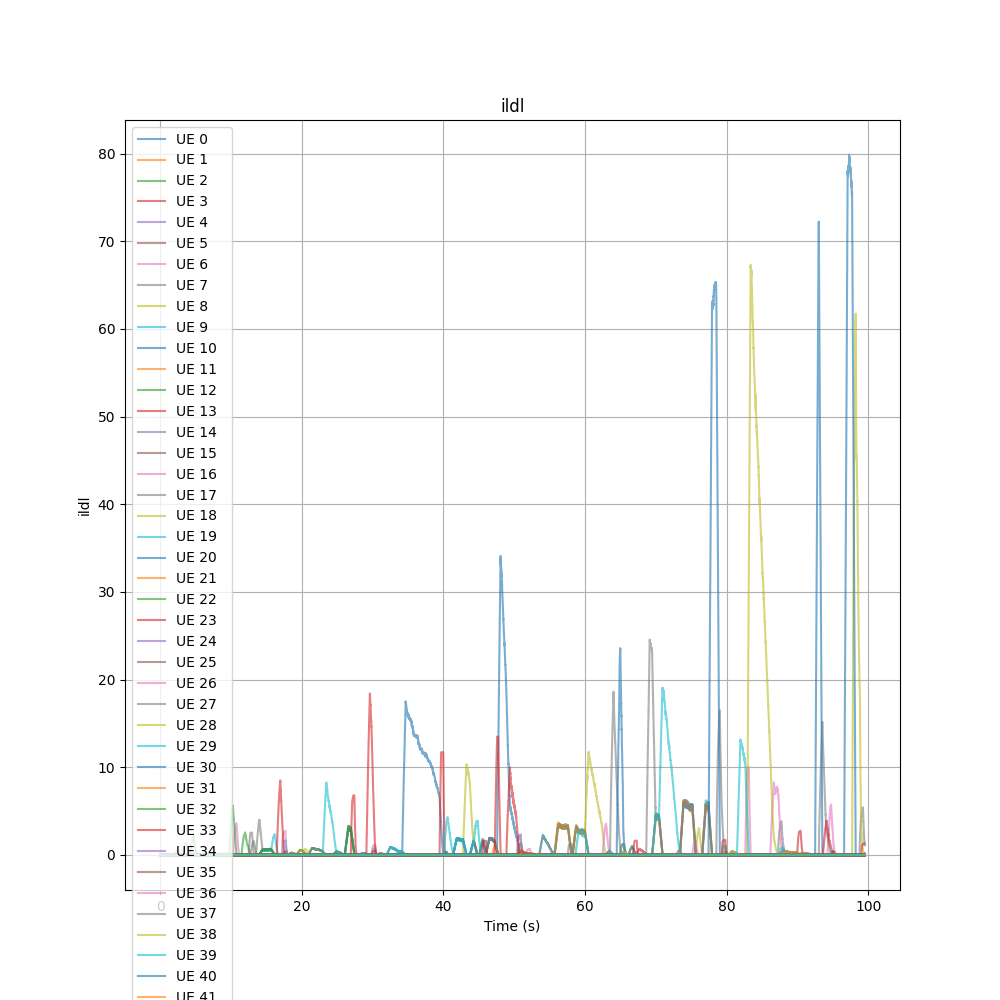
\includegraphics[scale=0.6]{../computos_y_graficas/scheduling_daneses_10mhz_3.5mbps_200ue/5_8_1_6_18/ue/ildl_instantaneous.png}}\end{center}

\begin{center}{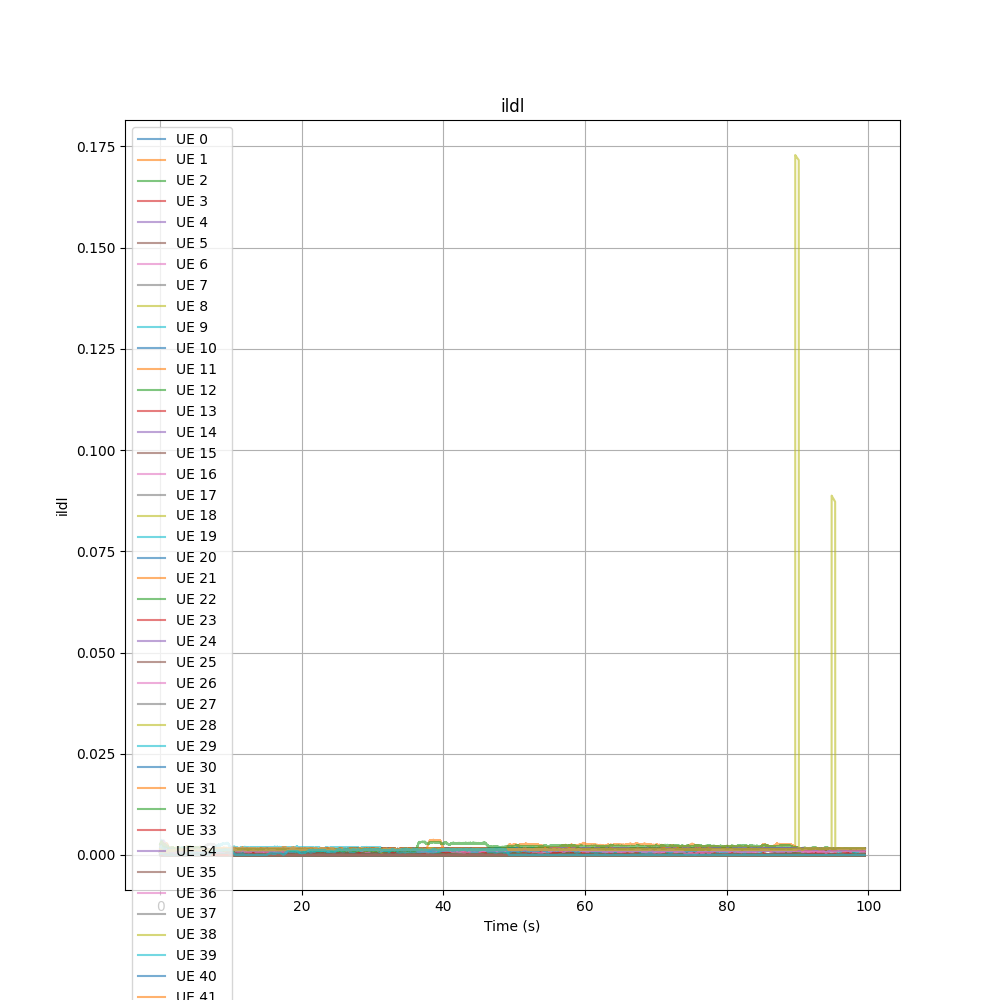
\includegraphics[scale=0.6]{../computos_y_graficas/scheduling_daneses_10mhz_3.5mbps_200ue/5_8_1_8_5/ue/ildl_instantaneous.png}}\end{center}

\begin{center}{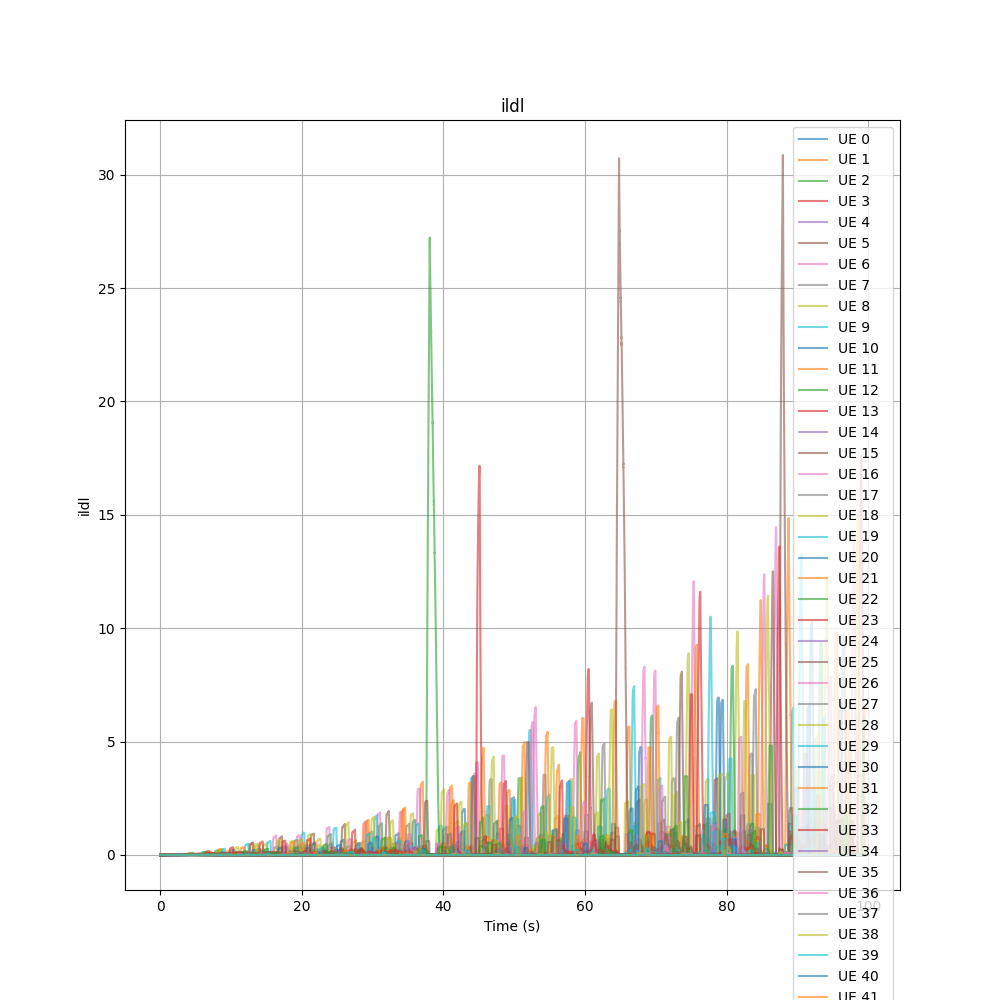
\includegraphics[scale=0.6]{../computos_y_graficas/scheduling_daneses_10mhz_3.5mbps_200ue/5_8_1_9_52/ue/ildl_instantaneous.png}}\end{center}

\begin{center}{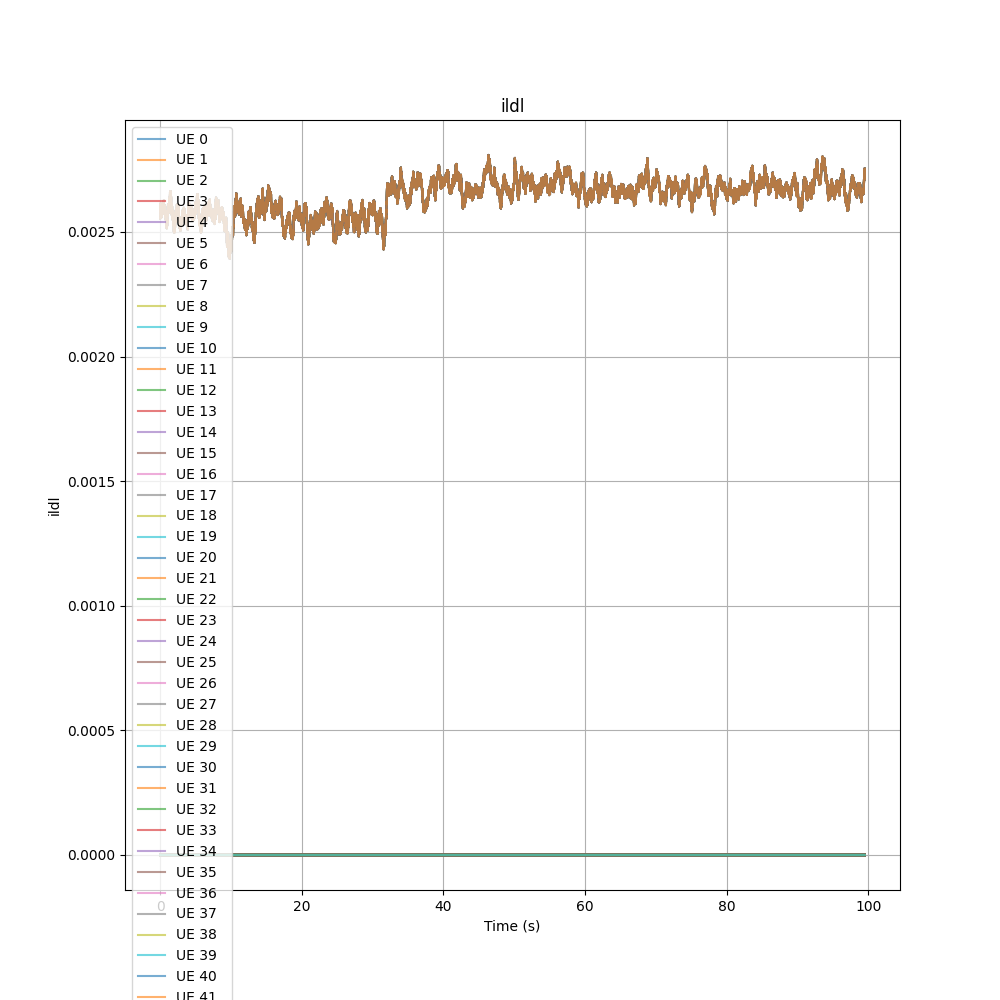
\includegraphics[scale=0.6]{../computos_y_graficas/scheduling_daneses_10mhz_3.5mbps_200ue/5_8_1_11_39/ue/ildl_instantaneous.png}}\end{center}

\begin{center}{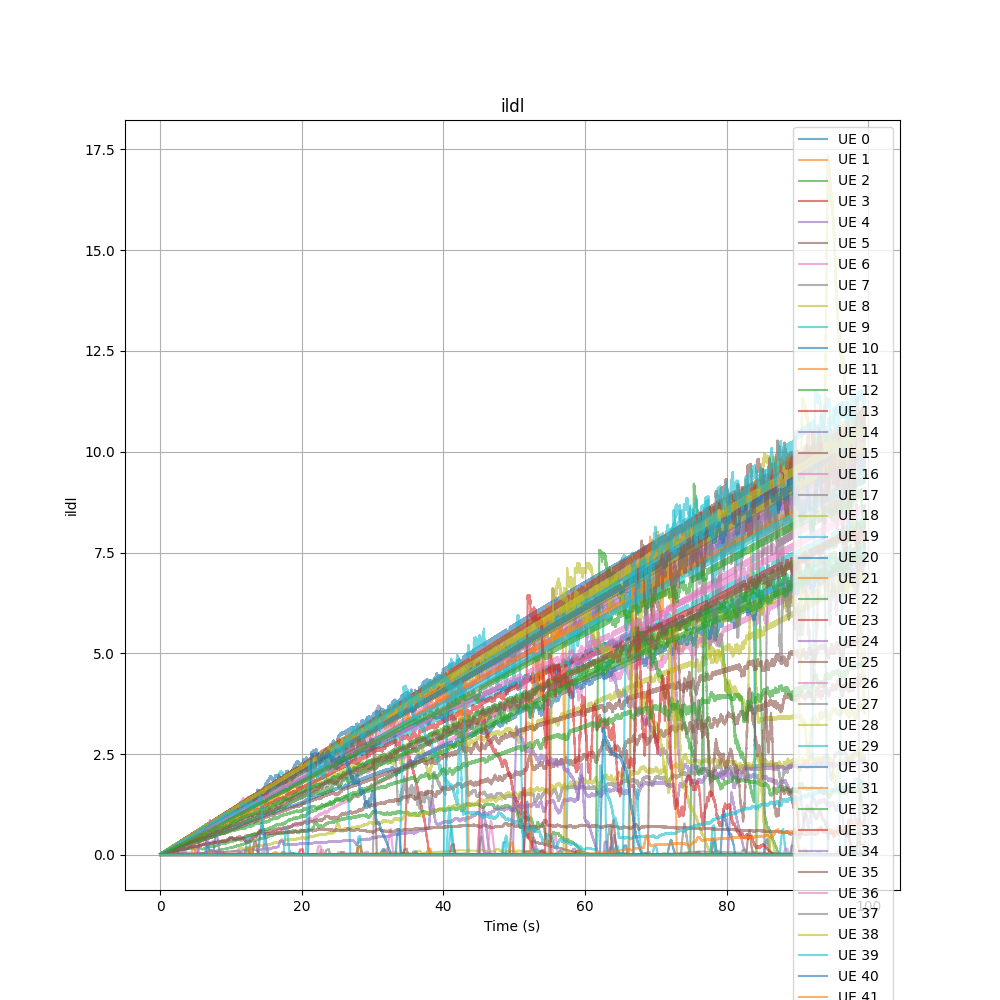
\includegraphics[scale=0.6]{../computos_y_graficas/scheduling_daneses_10mhz_3.5mbps_200ue/5_8_1_13_26/ue/ildl_instantaneous.png}}\end{center}

\begin{center}{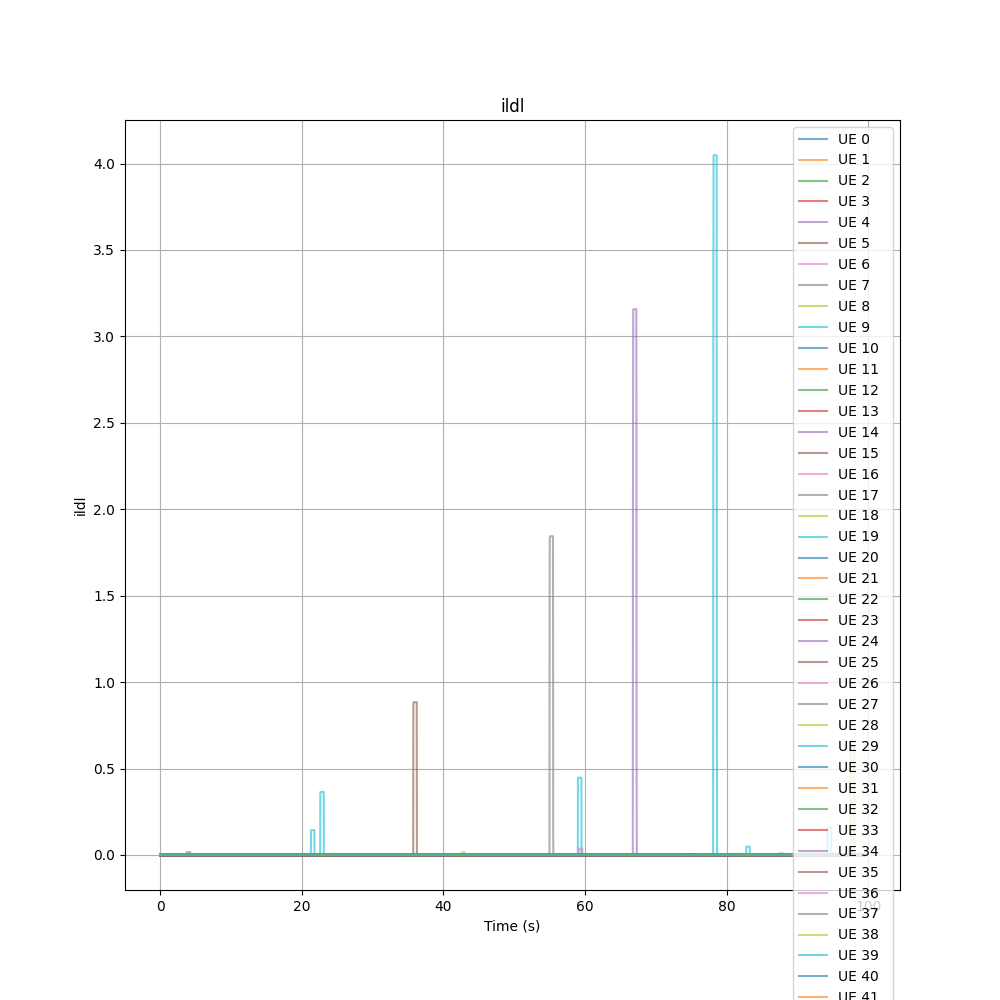
\includegraphics[scale=0.6]{../computos_y_graficas/scheduling_daneses_10mhz_3.5mbps_200ue/5_8_1_15_13/ue/ildl_instantaneous.png}}\end{center}

\begin{figure}[H]
	\ffigbox[\FBwidth] {
	\caption[Planificación de paquetes - Tercer caso - Latencia instantánea (I)]{Latencia de los paquetes IP en dirección DL usando distintas métricas
	(simulación con 200 UE).

	(Fila 1): FIFO.

	(Fila 2): BET.

	(Fila 3): EDF.

	(Fila 4): LWDF.

	(Fila 5): MT.

	(Fila 6): RR.

	(Fila 7): PF.

	(Fila 8): M-LWDF.}
	}
	{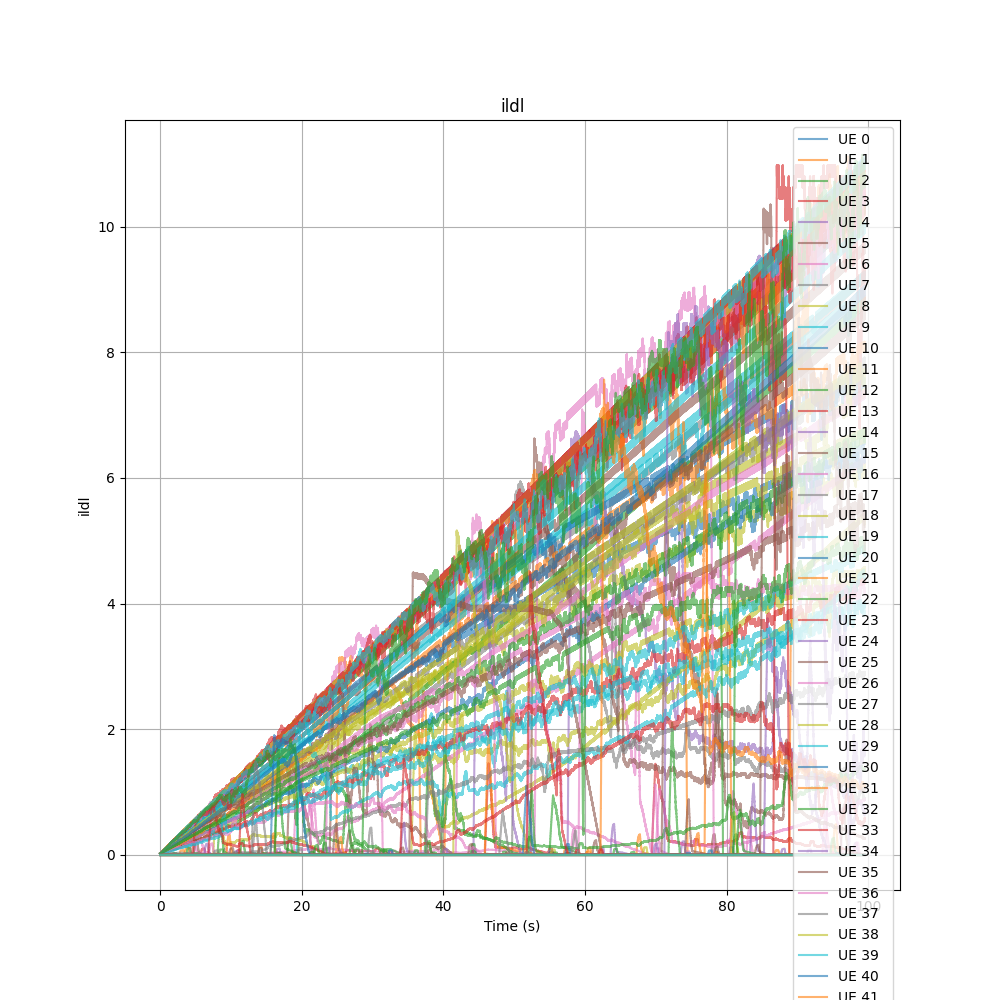
\includegraphics[scale=0.6]{../computos_y_graficas/scheduling_daneses_10mhz_3.5mbps_200ue/5_8_1_17_0/ue/ildl_instantaneous.png}}
\end{figure}

A continuación, estudiamos la latencia de los paquetes IP, que aparece en la figura 4.27.
En paralelo a que en FIFO y LWDF la tasa de error se estabilice en valores bajos,
la latencia va creciendo;
FIFO es una métrica sencilla que no está centrada en cuidar de la latencia,
pero LWDF sí está diseñada para ello, por lo que no se ha configurado adecuadamente para este experimento.
BET, EDF y PF mantienen latencias bajas, con picos repentinos de UE que quedan sin atender;
como explicamos, en ninguna de esas métricas se cuida la llegada a un tiempo límite, por lo que es esperable que haya entidades de UE que deban esperar a ser servidas.
RR y  M-LWDF muestran un progresivo crecimiento de la latencia para algunos UE;
RR no está diseñada para controlar la latencia,
mientras que M-LWDF sí, pero no ha sido debidamente configurada para este experimento.
MT muestra una latencia estable, en unos UE baja y en otros más alta;
MT atiende con mayor prioridad a los UE con mejor canal y ésta se refleja en la latencia estable.

%{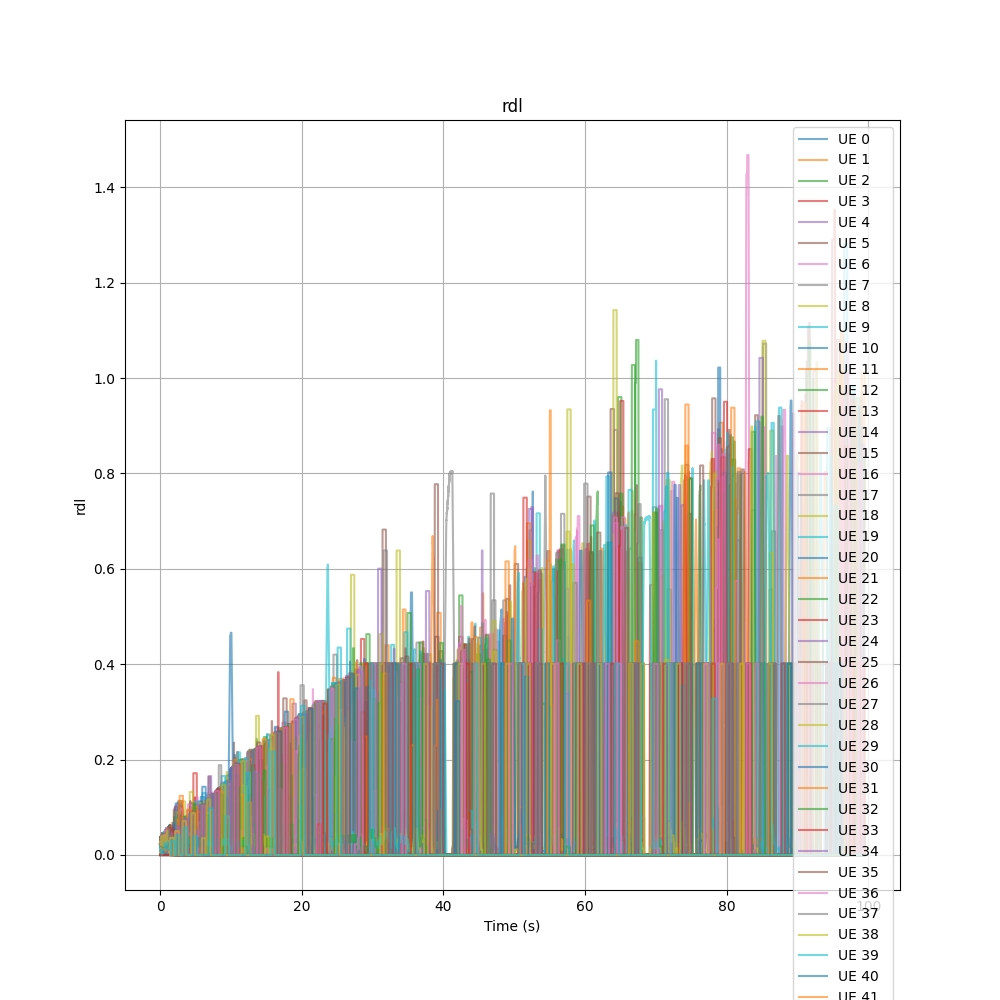
\includegraphics[scale=0.6]{../computos_y_graficas/scheduling_daneses_10mhz_3.5mbps_200ue/5_8_1_4_32/ue/rdl_instantaneous.png}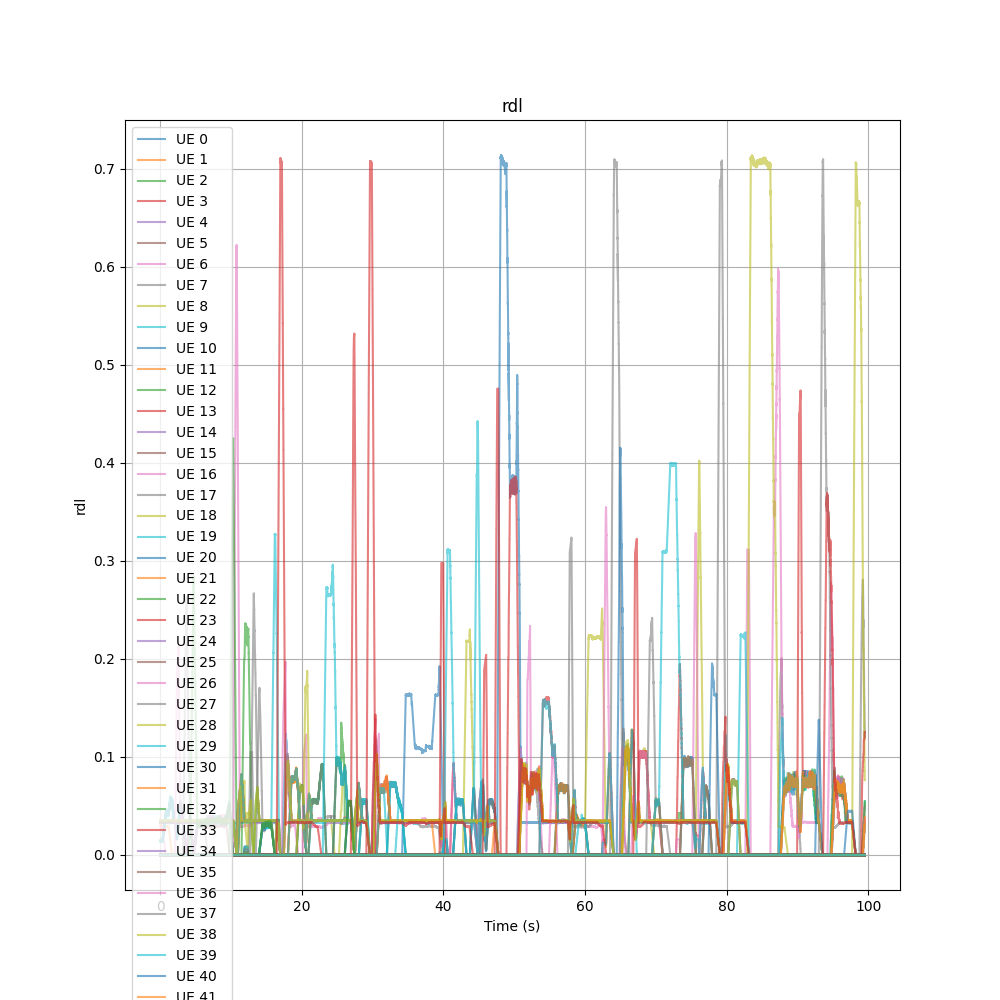
\includegraphics[scale=0.6]{../computos_y_graficas/scheduling_daneses_10mhz_3.5mbps_200ue/5_8_1_6_18/ue/rdl_instantaneous.png}}
%
%{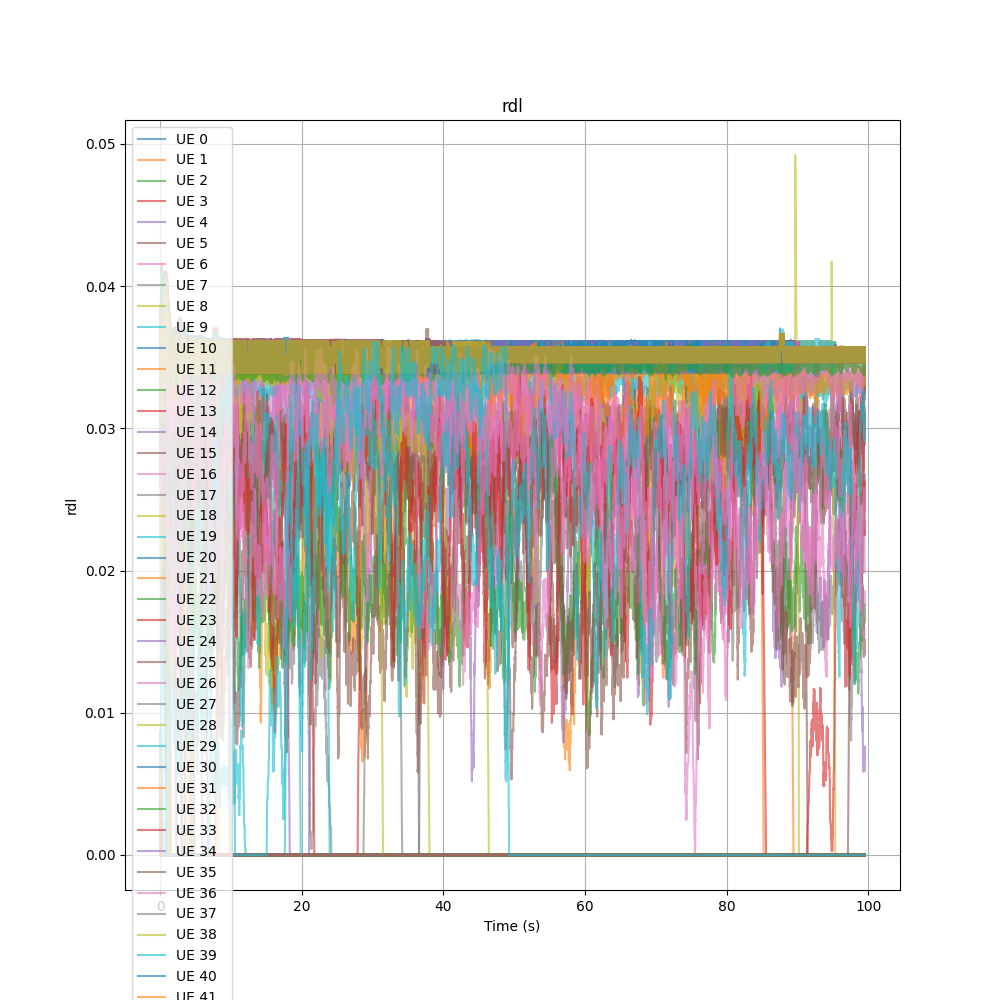
\includegraphics[scale=0.6]{../computos_y_graficas/scheduling_daneses_10mhz_3.5mbps_200ue/5_8_1_8_5/ue/rdl_instantaneous.png}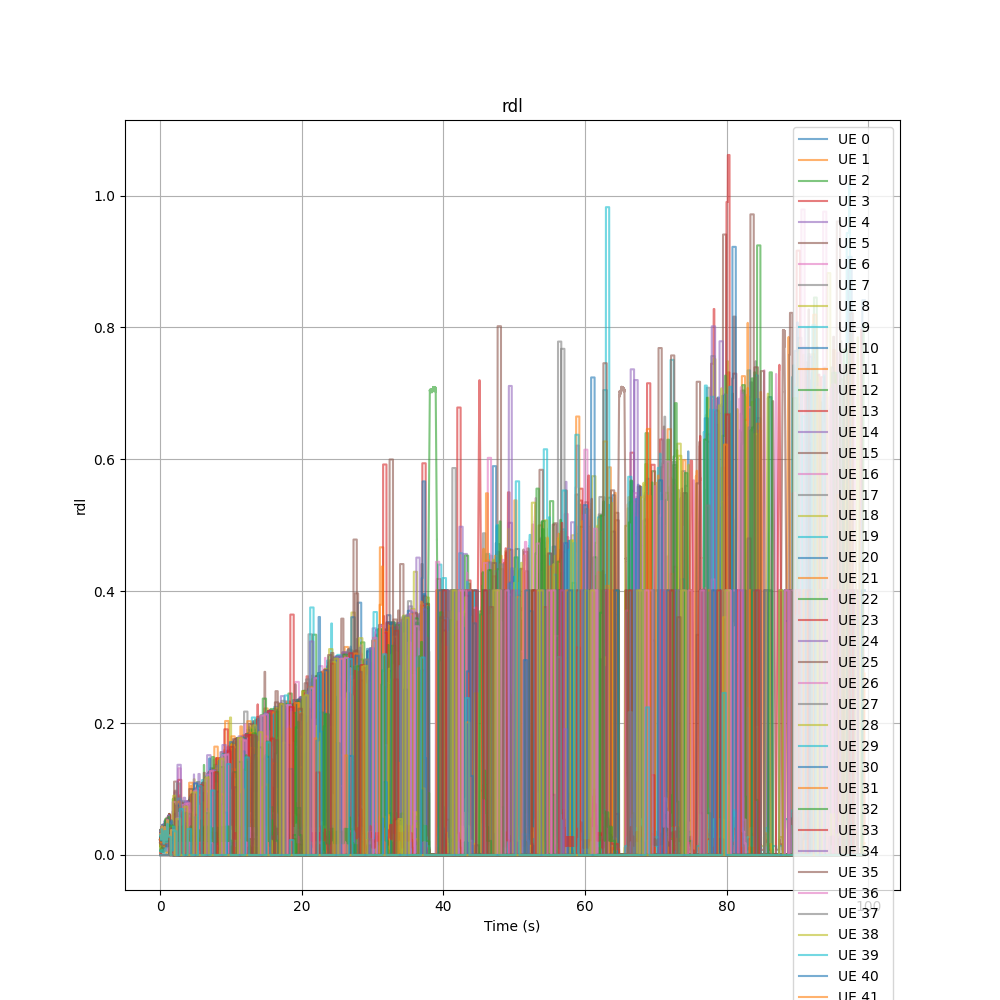
\includegraphics[scale=0.6]{../computos_y_graficas/scheduling_daneses_10mhz_3.5mbps_200ue/5_8_1_9_52/ue/rdl_instantaneous.png}}
%
%{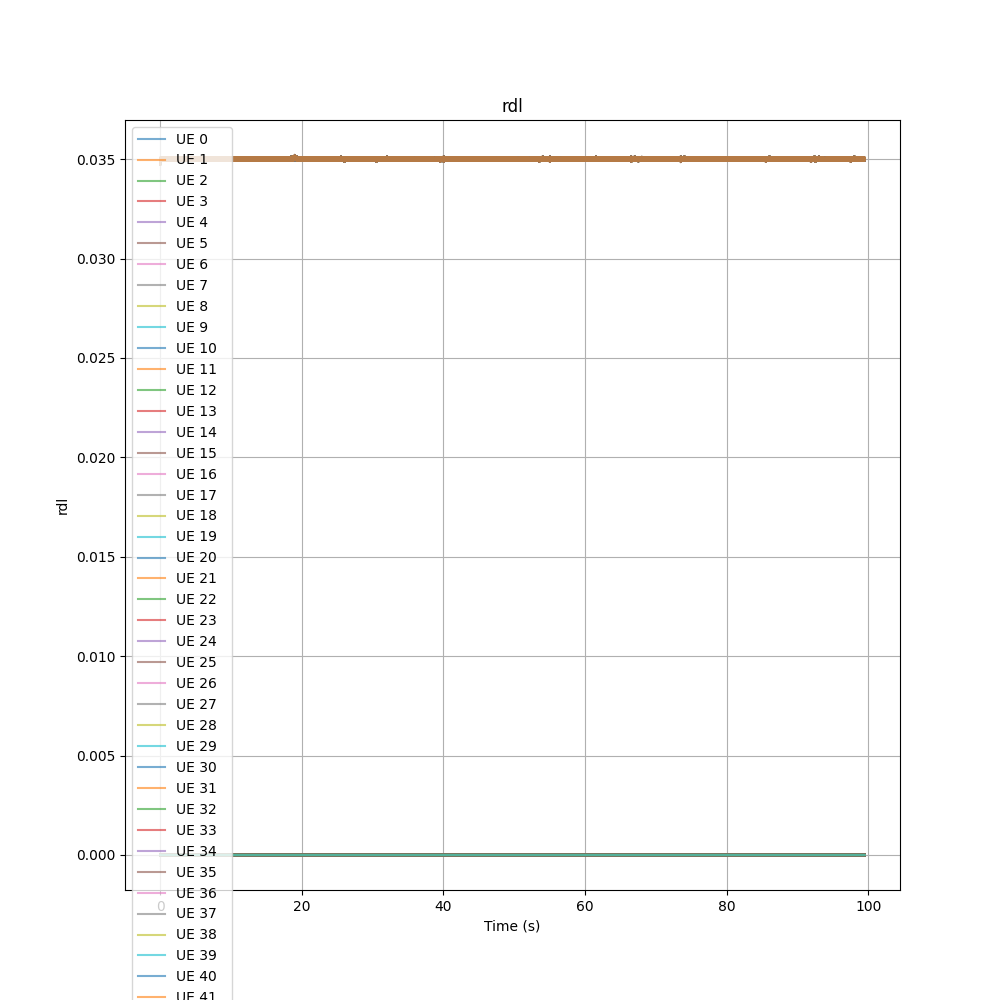
\includegraphics[scale=0.6]{../computos_y_graficas/scheduling_daneses_10mhz_3.5mbps_200ue/5_8_1_11_39/ue/rdl_instantaneous.png}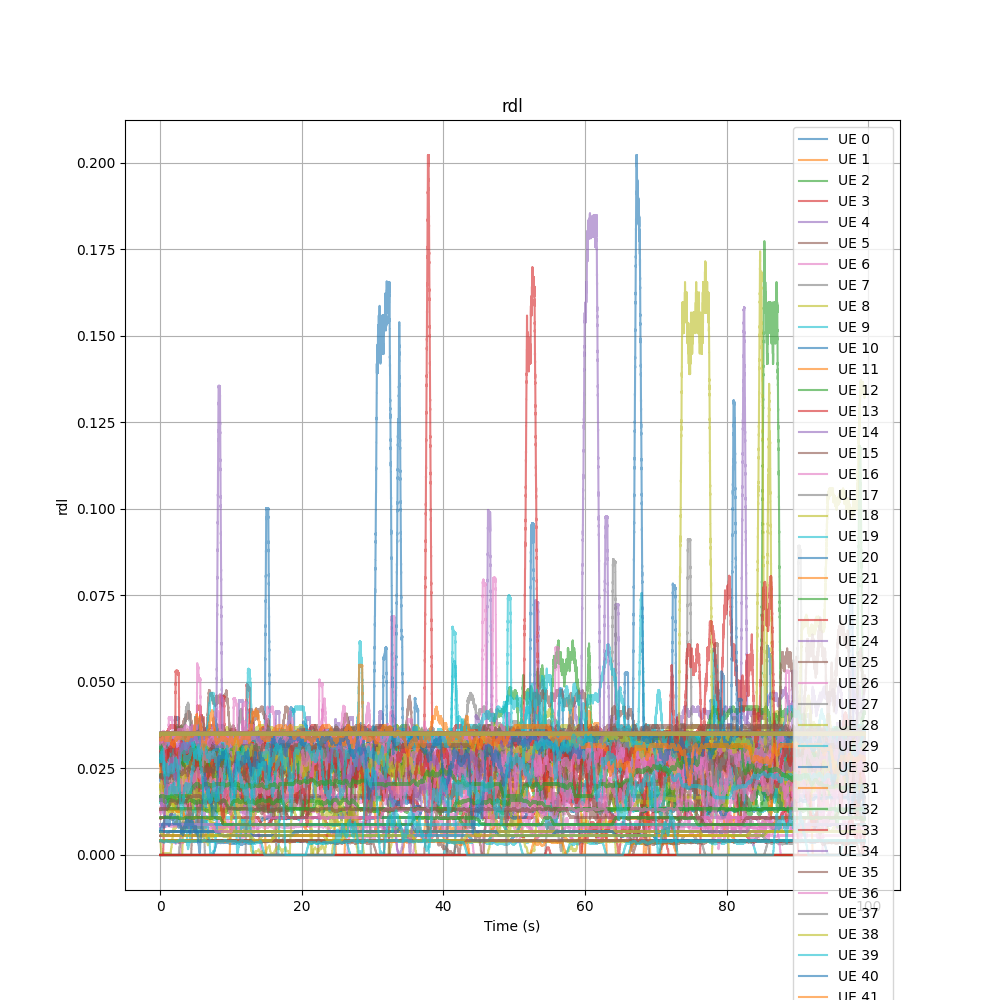
\includegraphics[scale=0.6]{../computos_y_graficas/scheduling_daneses_10mhz_3.5mbps_200ue/5_8_1_13_26/ue/rdl_instantaneous.png}}
%
%\begin{figure}[H]
%	\ffigbox[\FBwidth] {
%	\caption[Caso - Packet scheduling - Daneses]{Tasa binaria en tiempo real en dirección DL usando las métricas
%	FIFO (arriba a la izquierda),
%	BET (arriba a la derecha),
%	EDF (en medio, arriba a la izquierda),
%	LWDF (en medio, arriba a la derecha),
%	MT (en medio, abajo a la izquierda),
%	RR (en medio, abajo a la derecha),
%	PF (abajo a la izquierda),
%	M-LWDF (abajo a la derecha)
%%	desconocida (nivel más bajo)
%	(simulación con 200 UE).}
%	}
%	{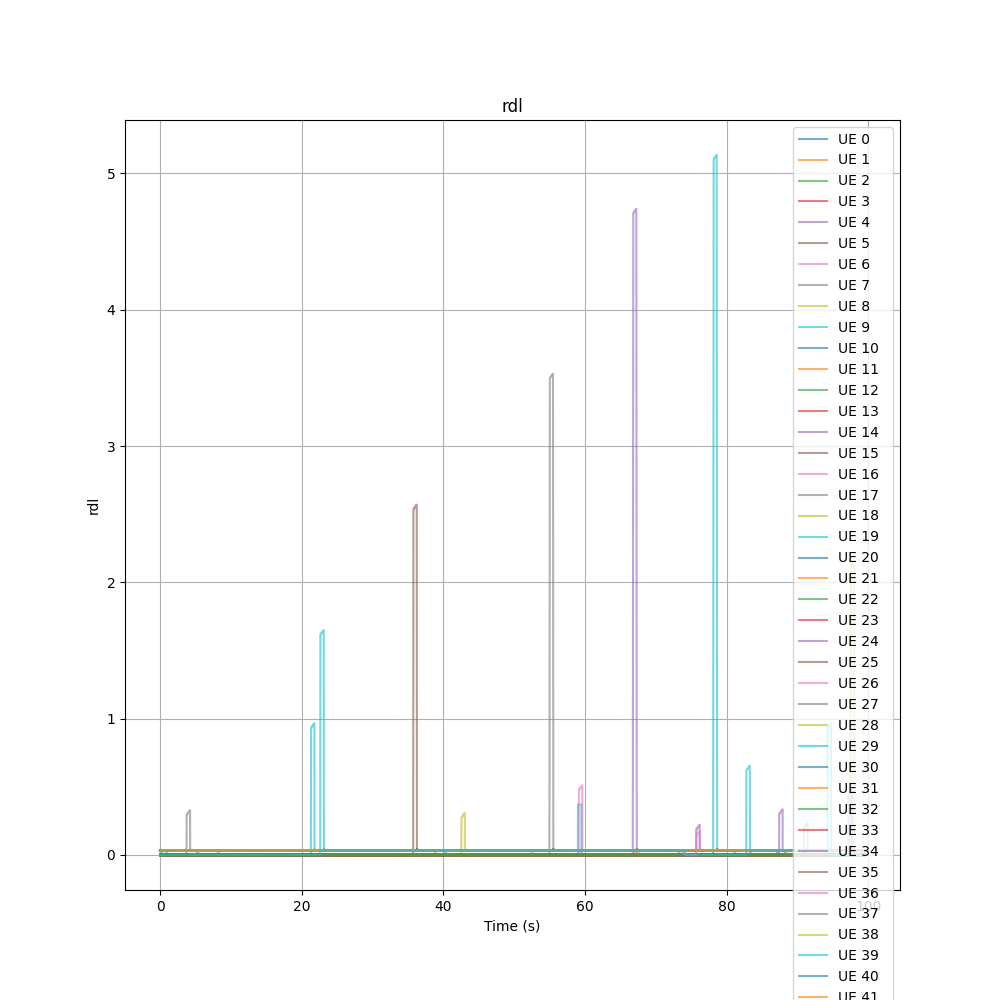
\includegraphics[scale=0.6]{../computos_y_graficas/scheduling_daneses_10mhz_3.5mbps_200ue/5_8_1_15_13/ue/rdl_instantaneous.png}
%	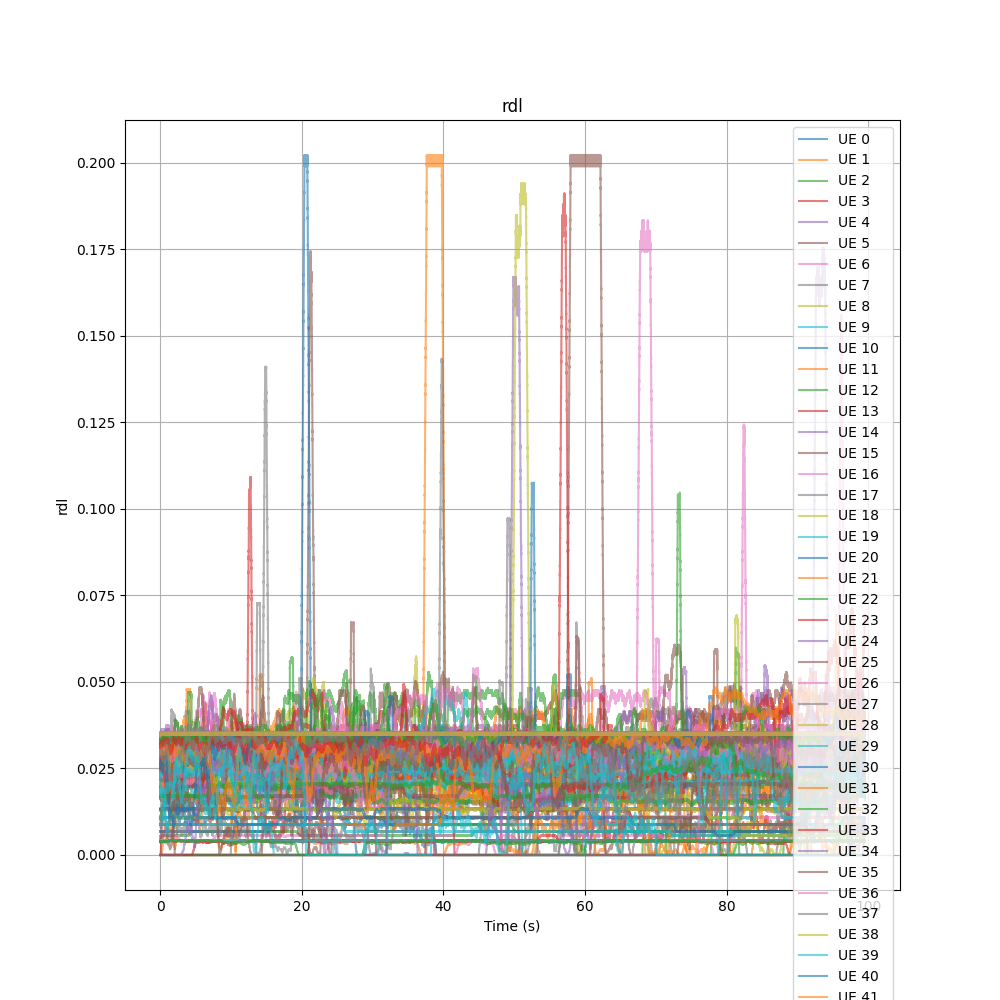
\includegraphics[scale=0.6]{../computos_y_graficas/scheduling_daneses_10mhz_3.5mbps_200ue/5_8_1_17_0/ue/rdl_instantaneous.png}}
%\end{figure}

\begin{center}{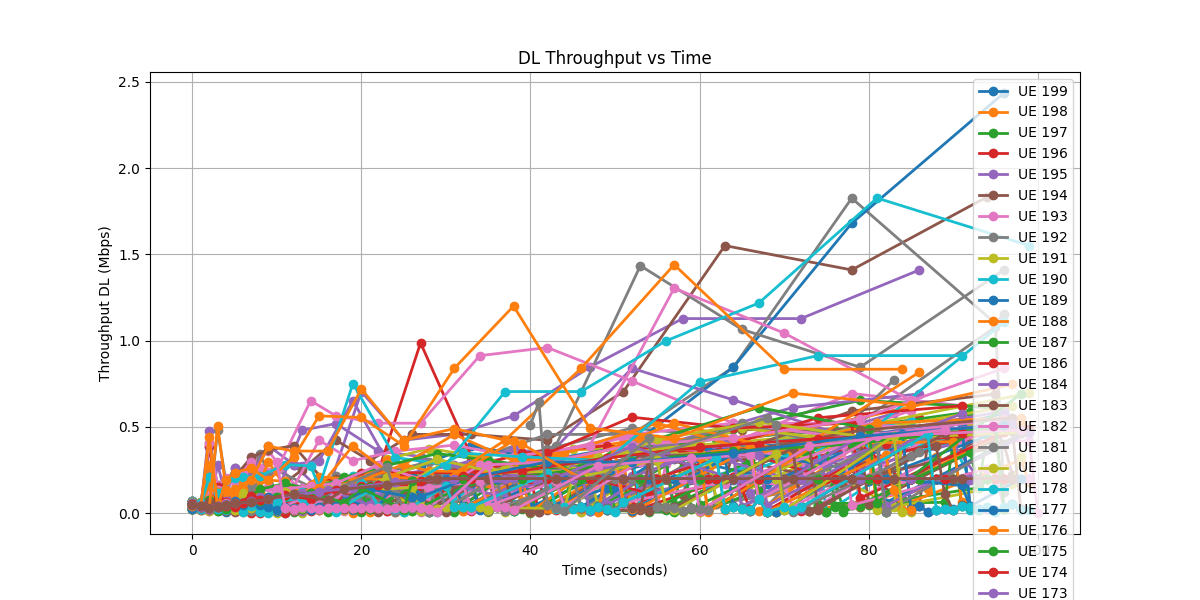
\includegraphics[scale=0.50]{../computos_y_graficas/scheduling_daneses_10mhz_3.5mbps_200ue/5_8_1_4_32/mac/dl_throughput.png}}\end{center}

\begin{center}{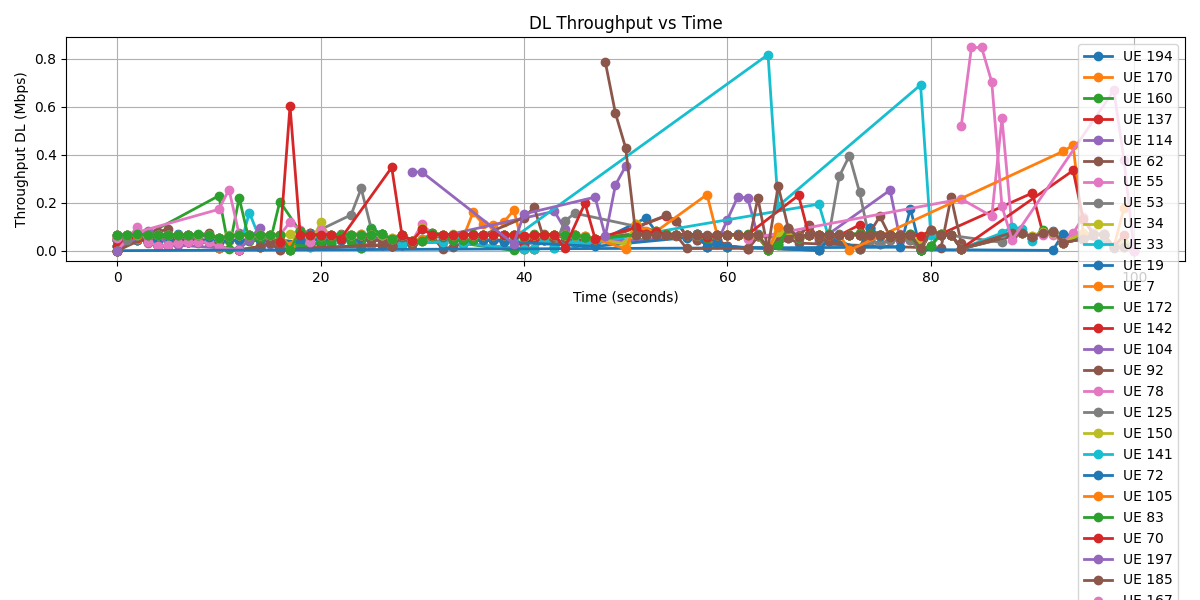
\includegraphics[scale=0.50]{../computos_y_graficas/scheduling_daneses_10mhz_3.5mbps_200ue/5_8_1_6_18/mac/dl_throughput.png}}\end{center}

\begin{center}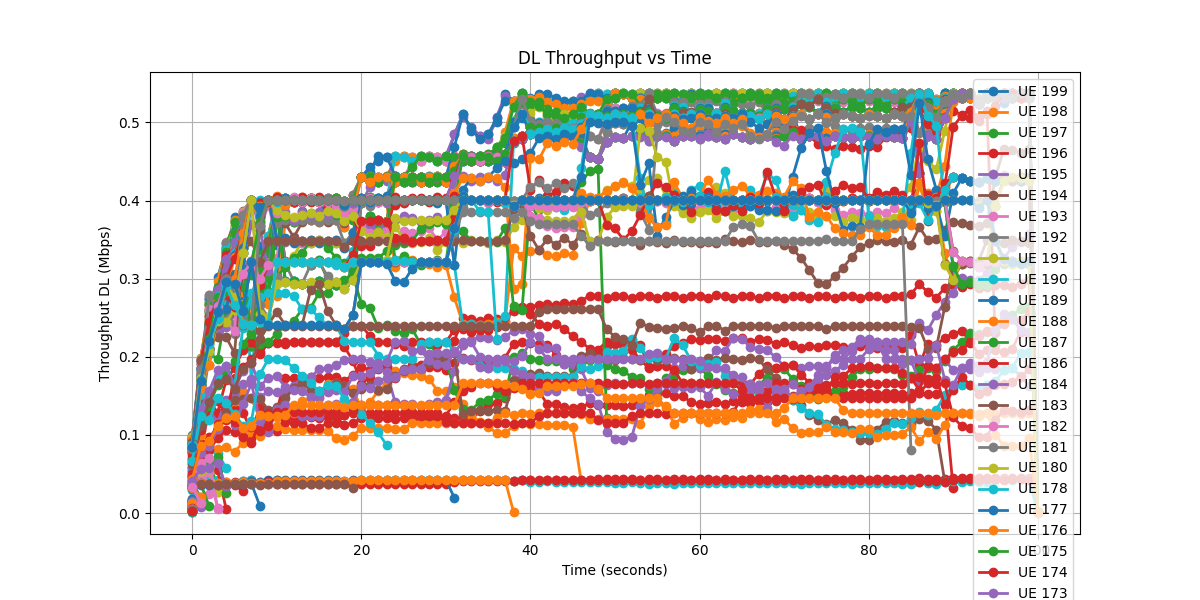
\includegraphics[scale=0.50]{../computos_y_graficas/scheduling_daneses_10mhz_3.5mbps_200ue/5_8_1_8_5/mac/dl_throughput.png}\end{center}

\begin{center}{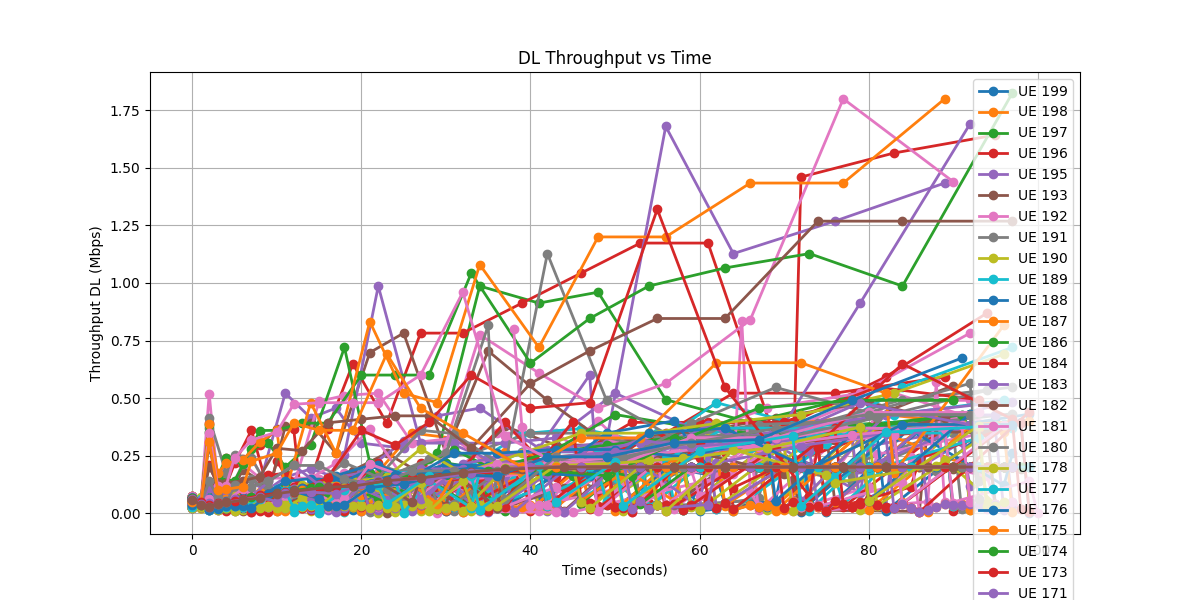
\includegraphics[scale=0.50]{../computos_y_graficas/scheduling_daneses_10mhz_3.5mbps_200ue/5_8_1_9_52/mac/dl_throughput.png}}\end{center}

\begin{center}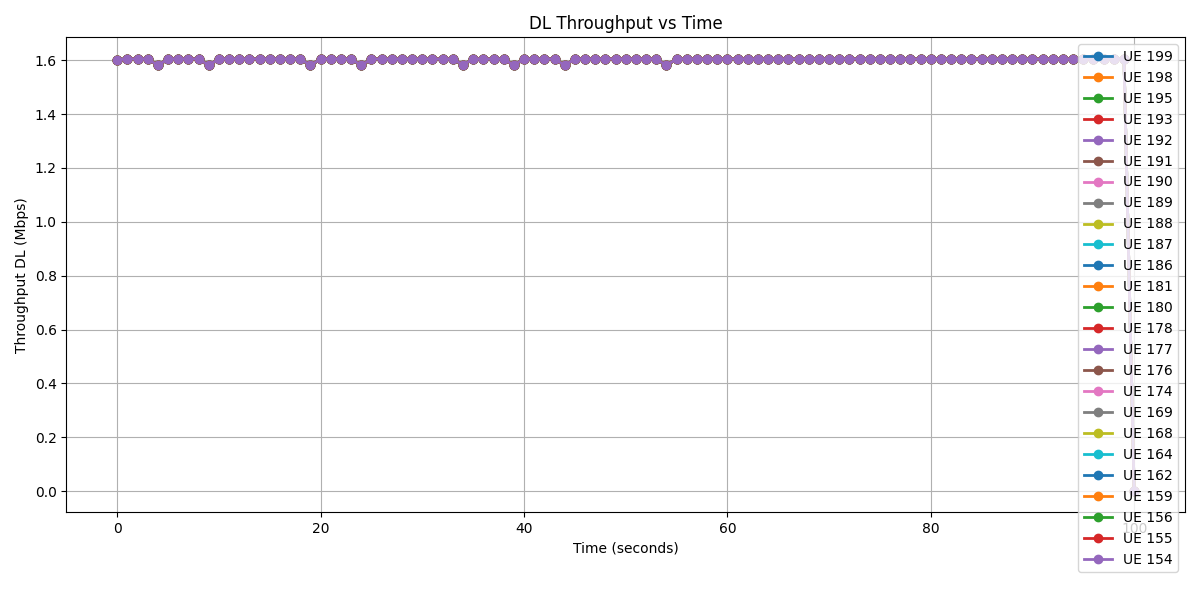
\includegraphics[scale=0.50]{../computos_y_graficas/scheduling_daneses_10mhz_3.5mbps_200ue/5_8_1_11_39/mac/dl_throughput.png}\end{center}

\begin{center}{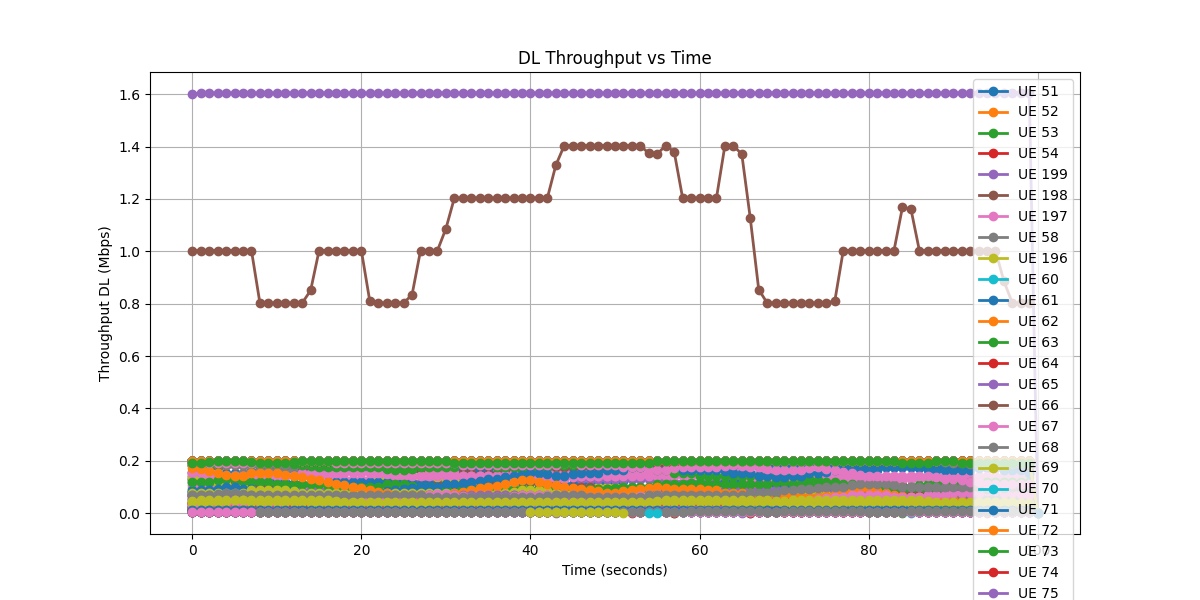
\includegraphics[scale=0.50]{../computos_y_graficas/scheduling_daneses_10mhz_3.5mbps_200ue/5_8_1_13_26/mac/dl_throughput.png}}\end{center}

\begin{center}{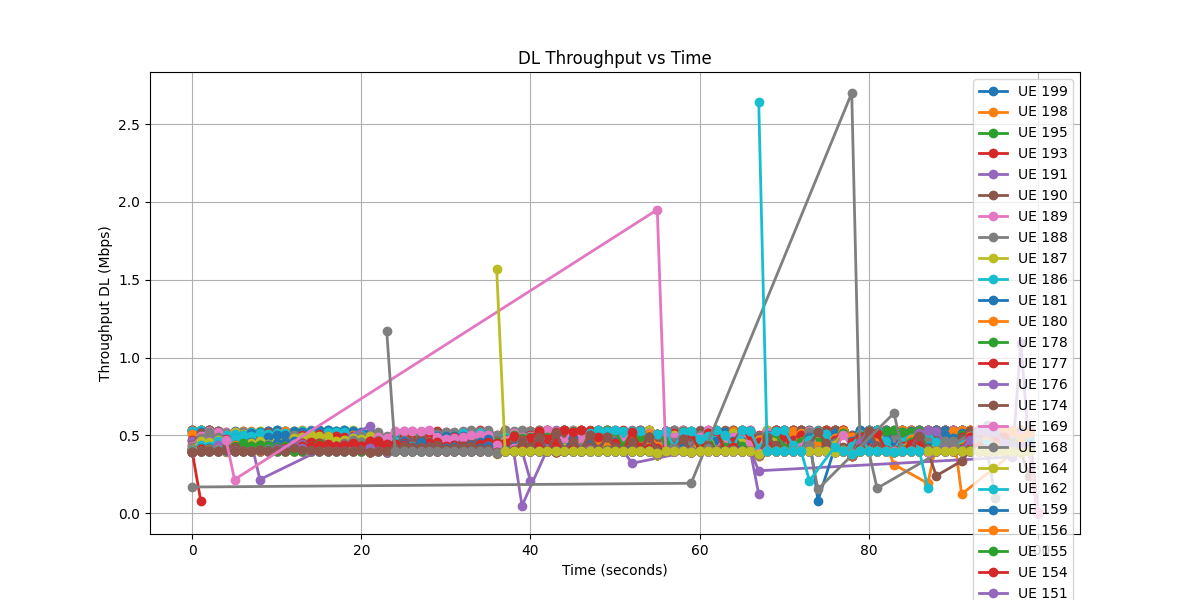
\includegraphics[scale=0.50]{../computos_y_graficas/scheduling_daneses_10mhz_3.5mbps_200ue/5_8_1_15_13/mac/dl_throughput.png}}\end{center}

\begin{figure}[H]
	\ffigbox[\FBwidth] {
	\caption[Planificación de paquetes - Tercer caso - Tasa binaria instantánea por UE (I)]{Tasa binaria en tiempo real en dirección DL usando distintas métricas
	(simulación con 200 UE).

	(Fila 1): FIFO.

	(Fila 2): BET.

	(Fila 3): EDF.

	(Fila 4): LWDF.

	(Fila 5): MT.

	(Fila 6): RR.

	(Fila 7): PF.

	(Fila 8): M-LWDF.}
	}
	{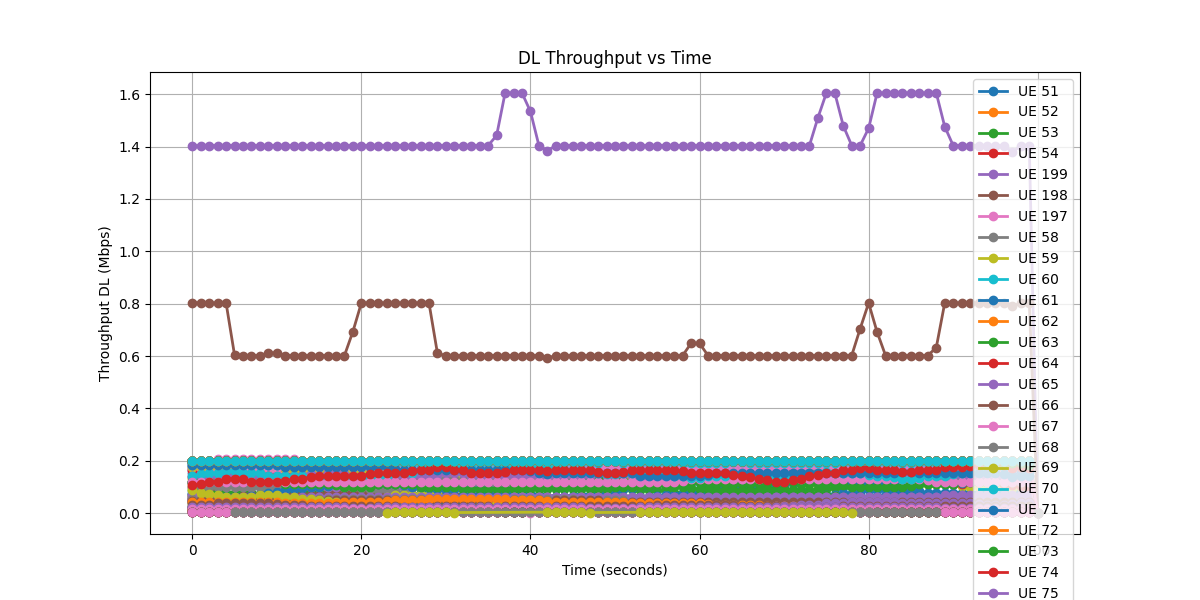
\includegraphics[scale=0.50]{../computos_y_graficas/scheduling_daneses_10mhz_3.5mbps_200ue/5_8_1_17_0/mac/dl_throughput.png}}
\end{figure}

\begin{center}{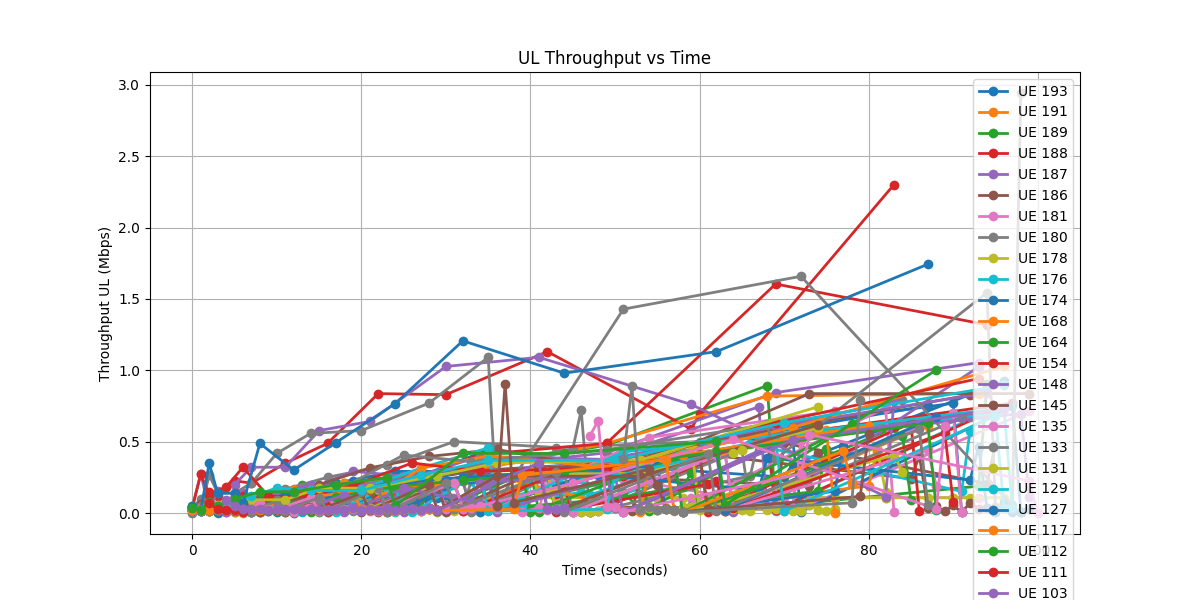
\includegraphics[scale=0.50]{../computos_y_graficas/scheduling_daneses_10mhz_3.5mbps_200ue/5_8_1_4_32/mac/ul_throughput.png}}\end{center}

\begin{center}{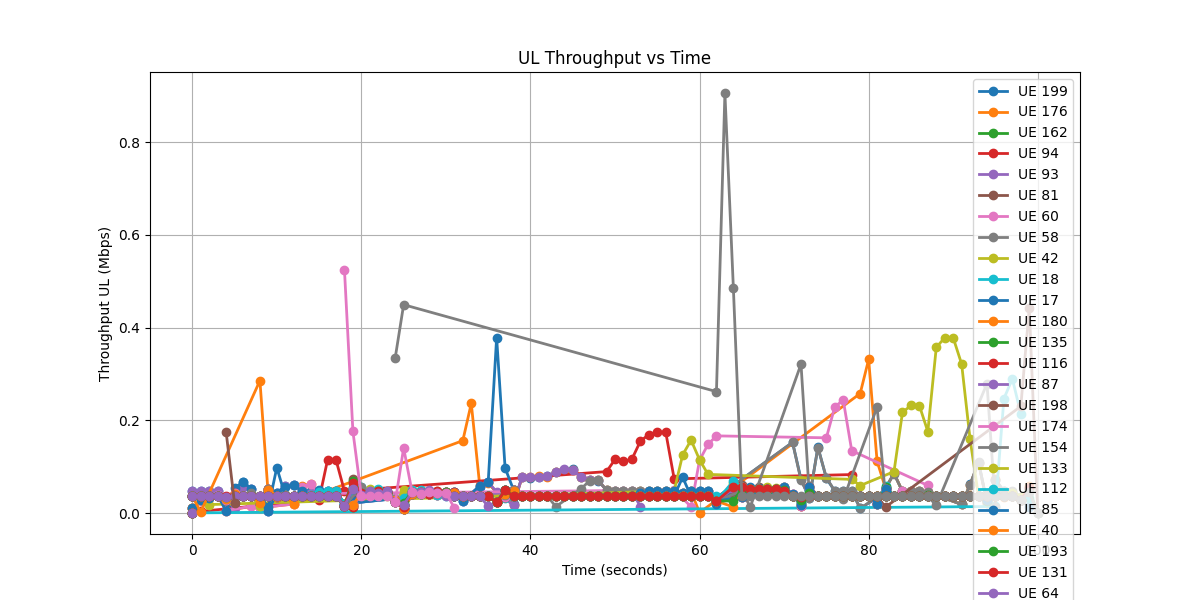
\includegraphics[scale=0.50]{../computos_y_graficas/scheduling_daneses_10mhz_3.5mbps_200ue/5_8_1_6_18/mac/ul_throughput.png}}\end{center}

\begin{center}{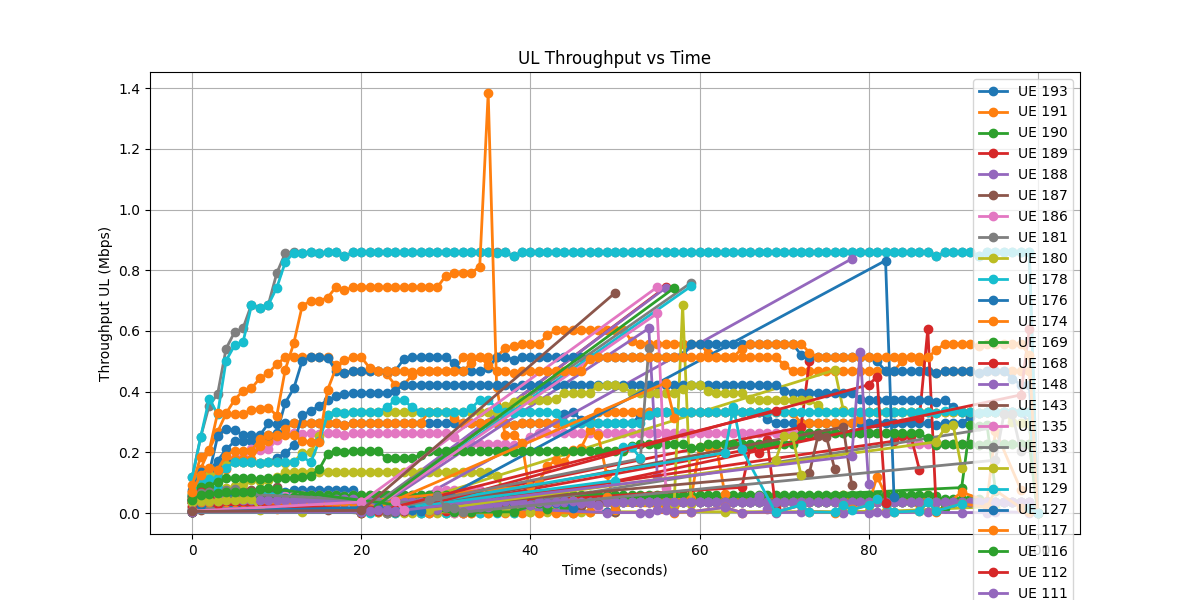
\includegraphics[scale=0.50]{../computos_y_graficas/scheduling_daneses_10mhz_3.5mbps_200ue/5_8_1_8_5/mac/ul_throughput.png}}\end{center}

\begin{center}{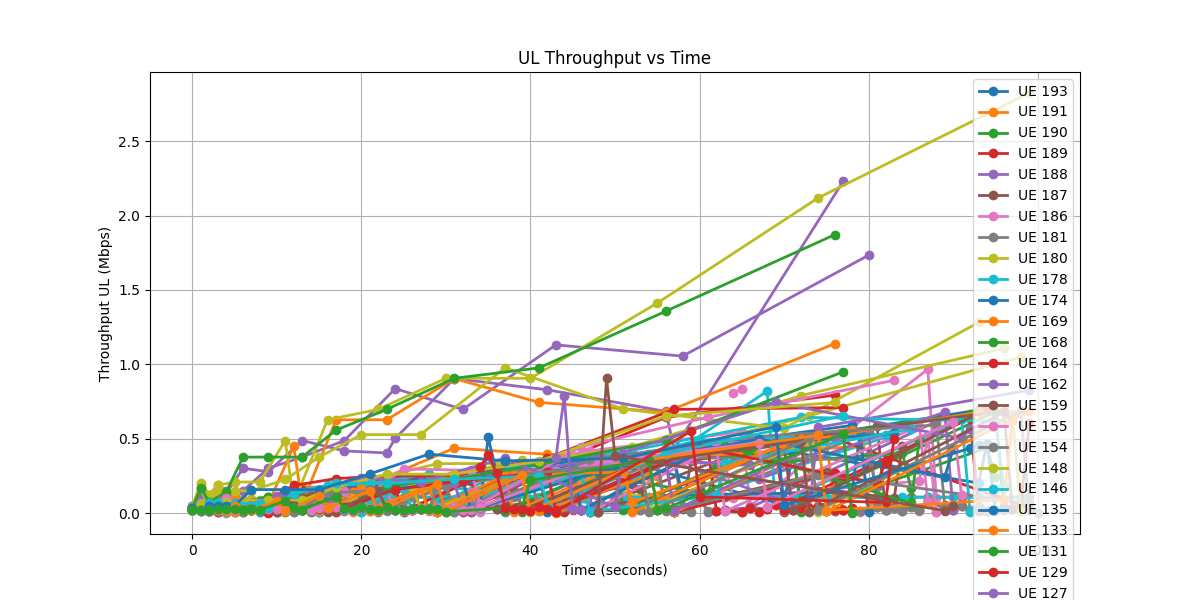
\includegraphics[scale=0.50]{../computos_y_graficas/scheduling_daneses_10mhz_3.5mbps_200ue/5_8_1_9_52/mac/ul_throughput.png}}\end{center}

\begin{center}{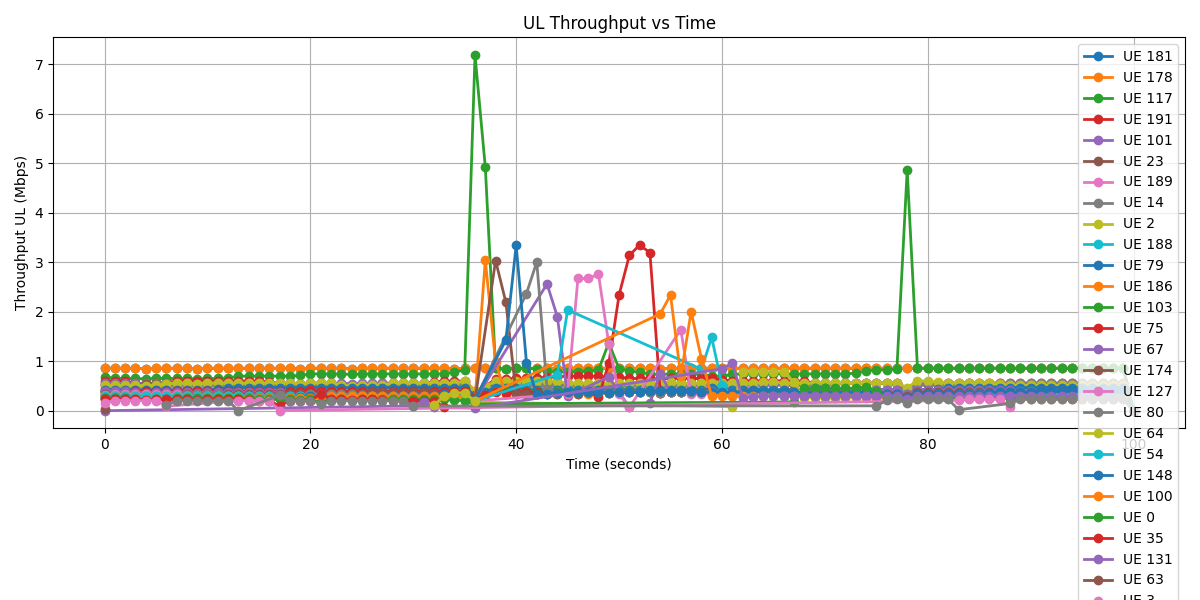
\includegraphics[scale=0.50]{../computos_y_graficas/scheduling_daneses_10mhz_3.5mbps_200ue/5_8_1_11_39/mac/ul_throughput.png}}\end{center}

\begin{center}{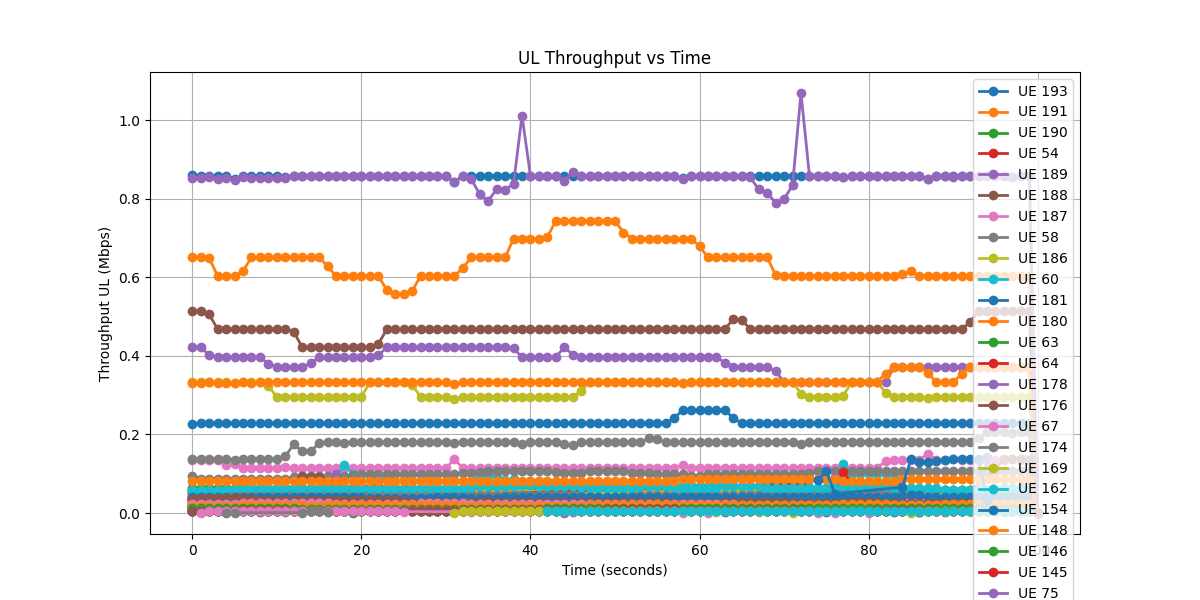
\includegraphics[scale=0.50]{../computos_y_graficas/scheduling_daneses_10mhz_3.5mbps_200ue/5_8_1_13_26/mac/ul_throughput.png}}\end{center}

\begin{center}{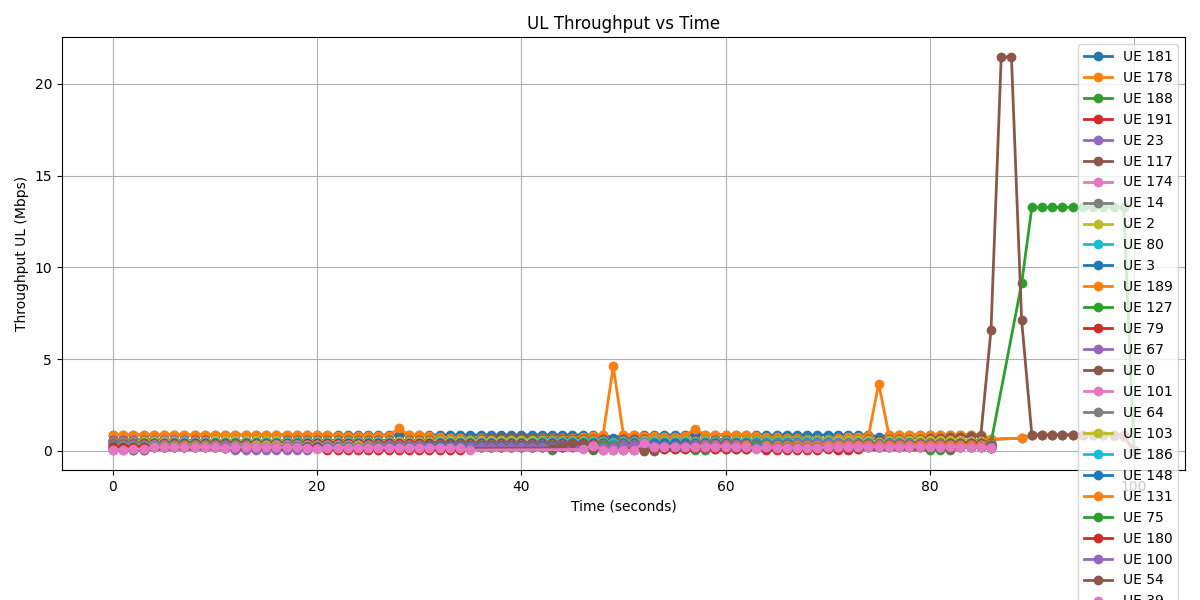
\includegraphics[scale=0.50]{../computos_y_graficas/scheduling_daneses_10mhz_3.5mbps_200ue/5_8_1_15_13/mac/ul_throughput.png}}\end{center}

\begin{figure}[H]
	\ffigbox[\FBwidth] {
	\caption[Planificación de paquetes - Tercer caso - Tasa binaria instantánea por UE (II)]{Tasa binaria en tiempo real en dirección UL usando distintas métricas
	(simulación con 200 UE).

	(Fila 1): FIFO.

	(Fila 2): BET.

	(Fila 3): EDF.

	(Fila 4): LWDF.

	(Fila 5): MT.

	(Fila 6): RR.

	(Fila 7): PF.

	(Fila 8): M-LWDF.}
	}
	{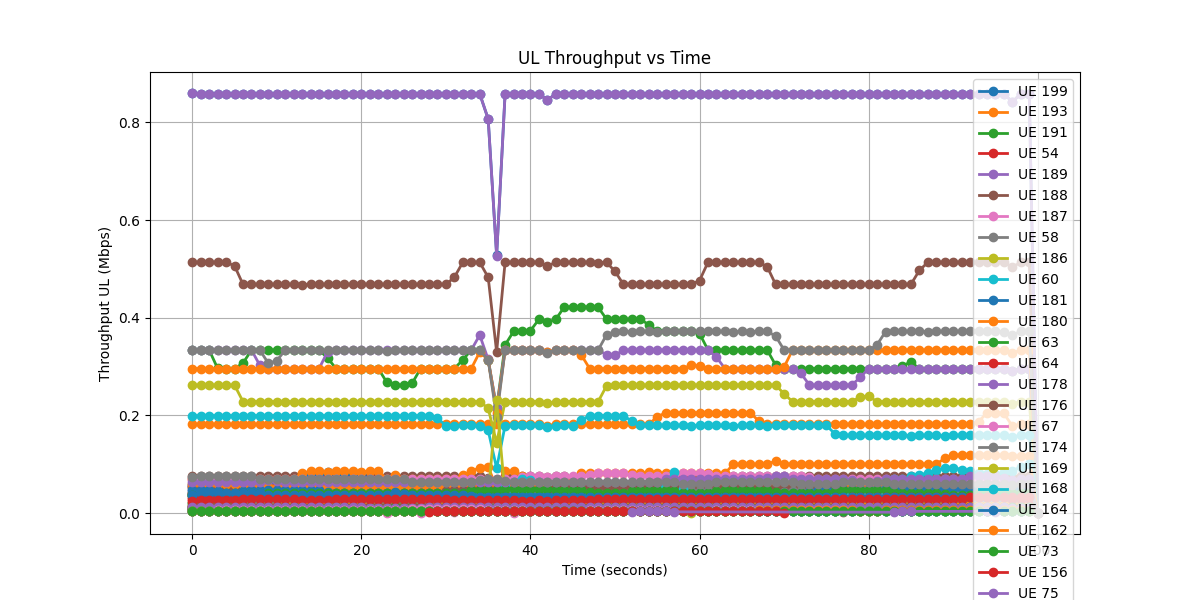
\includegraphics[scale=0.50]{../computos_y_graficas/scheduling_daneses_10mhz_3.5mbps_200ue/5_8_1_17_0/mac/ul_throughput.png}}
\end{figure}



Por último, vemos la tasa binaria de cada UE en las figuras 4.28 y 4.29.
En paralelo a que en FIFO y LWDF la tasa de error se estabilice en valores bajos y que la latencia crezca, su tasa binaria también lo hace;
ambas métricas asignan recursos sin la prioridad exclusiva de elevar la tasa,
FIFO es una métrica sencilla y LWDF no se ha configurado para reducir la latencia.
BET y PF asignan recursos por igual a todos los UE;
ambas métricas se han diseñado para mantener la justicia en el sistema.
MT, RR, EDF y M-LWDF dan un reparto más desigual;
MT está diseñada para maximizar la tasa binaria, favoreciendo a los UE con mejor canal;
M-LWDF está diseñada para lograr cierta eficiencia espectral, ocasionando un comportamiento similar al de MT;
EDF no tiene como objetivo principal la justicia, sino la latencia, por lo que también crea desigualdades;
RR atiende a los UE por orden, resultando en que se asignen recursos de manera desigual.

\subsection{Comparación de métricas en \textit{FikoRE} y en \textit{5G-LENA/NS-3}}

\subsubsection{Introducción}

El artículo \cite{RefWorks:67} se centra en las métricas usadas en el planificador.
Usa los módulos de NR de \textit{5G-LENA} con el simulador \textit{NS-3}.
También propone una métrica novedosa, \textit{Optimized PF}, que pretende mantener elevadas prestaciones de tasa binaria y justicia en la asignación de recursos.
También estudia el efecto de usar distintas numerologías.

Los experimentos propuestos se pueden simular y para comparar los resultados obtenidos con \textit{NS-3} con los de \textit{FikoRE}.
Se puede llegar a conclusiones relativas al diseño del planificador.

Se ha representado el experimento con \textit{FikoRE}
(véase \textit{Caso de uso (IX): packet scheduling (indonesios)} en el anexo \textit{Simulaciones (metadatos)}).

\subsubsection{Descripción del experimento 1: métricas}

Se proponen varios experimentos en los que se simula un número distinto de UE conectados (1, 5, 10, 20, 30).
Se simulan las numerologías 0 y 4.
Se simulan las métricas RR, MT, PF y \textit{Optimized PF}.
El resto de características se indican en la tabla 4.3.

\begin{table}[H]
	\ttabbox[\FBwidth]
	{\caption{Planificación de paquetes - Cuarto caso - Características del experimento propuesto}}
	{\begin{tabular}{|P{3.0cm}|P{10cm}|}
		\hline
		\textbf{Parámetro} & \textbf{Valor} \\
		\hline
		Escenario & \textit{Urban Macro} (UMa) \\
		\hline
		Modelo de canal & 3GPP, LoS \\
		\hline
		Ancho de banda para DL & 200 MHz \\
		\hline
		Ancho de banda para UL & 100 MHz \\
		\hline
		Portadora & 28 GHz \\
		\hline
		Altura de la gNB & 10 m \\
		\hline
		Altura del UE & 1.5 m \\
		\hline
		Distancia & 10 m \\
		\hline
		Desvanecimiento lento & Deshabilitado \\
		\hline
		MCS & 28 \\
		\hline
		Latencia de codificación & 2 \textit{slots} \\
		\hline
		\multicolumn{2}{l}{Fuente: \cite{RefWorks:67}}
	\end{tabular}}
\end{table}

Se ha adaptado el mismo experimento para realizarse con el emulador \textit{FikoRE}:

\begin{itemize}
\item Se ha decidido simular únicamente la numerología 0.
\item \textit{FikoRE} sí simula el desvanecimiento lento, entre otros efectos, acorde con los modelos de canal descritos.
\item Se ha decidido simular un tráfico exigente: 150 Mbps en UL y 150 Mbps en DL para cada UE.
\item Se ha usado un movimiento circular alrededor de la gNB.
\item Se han probado las distintas métricas de las que disponía \textit{FikoRE}: FIFO, BET, EDF, LWDF, MT, RR, PF.
\item Para cada métrica, se ha simulado el número de UE indicado: 1, 5, 10, 20, 30.
\end{itemize}

\begin{figure}[H]
	\ffigbox[\FBwidth] {
	\caption[Planificación de paquetes - Cuarto caso - Nº. de UE (I)]{Número de UE en las distintas simulaciones.
	Las métricas por orden con el número de simulaciones entre paréntesis: FIFO (5), BET (5), EDF (5), LWDF (5), MT (5), RR (5), PF (5).}
	}
	{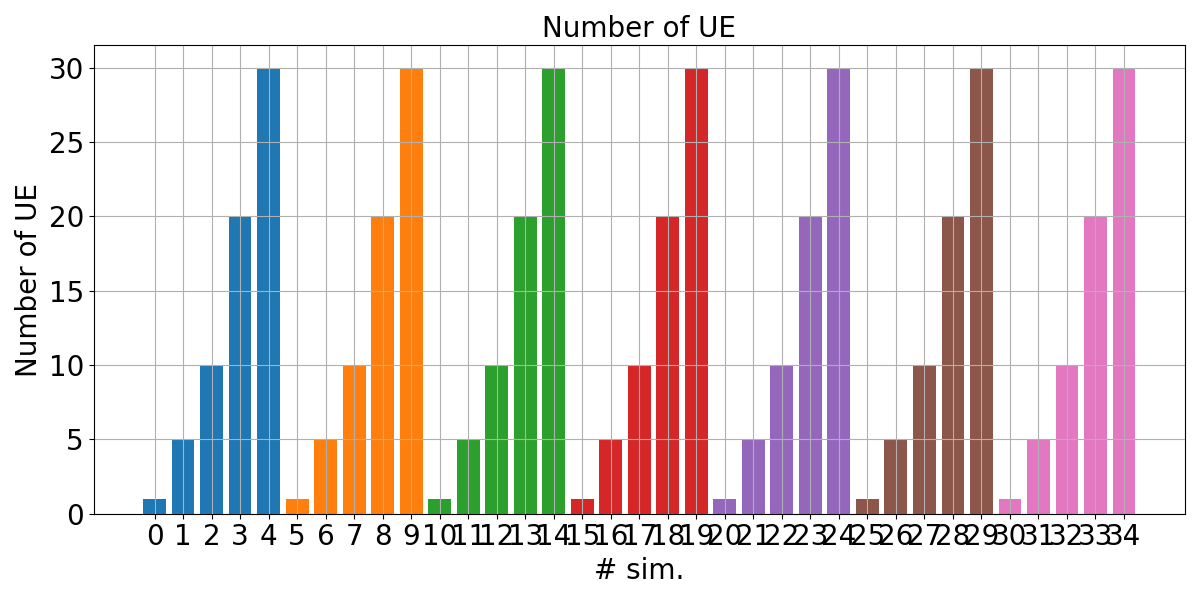
\includegraphics[scale=0.4]{../comparaciones/scheduling_indonesios_mu0_sin_prioridades/ue/n_ue_multi_sim.png}}
\end{figure}


\begin{figure}[H]
	\ffigbox[\FBwidth] {
	\caption[Planificación de paquetes - Cuarto caso - Trayectoria (I)]{Trayectoria seguida por las entidades de UE en una simulación con 10 UE.}
	}
	{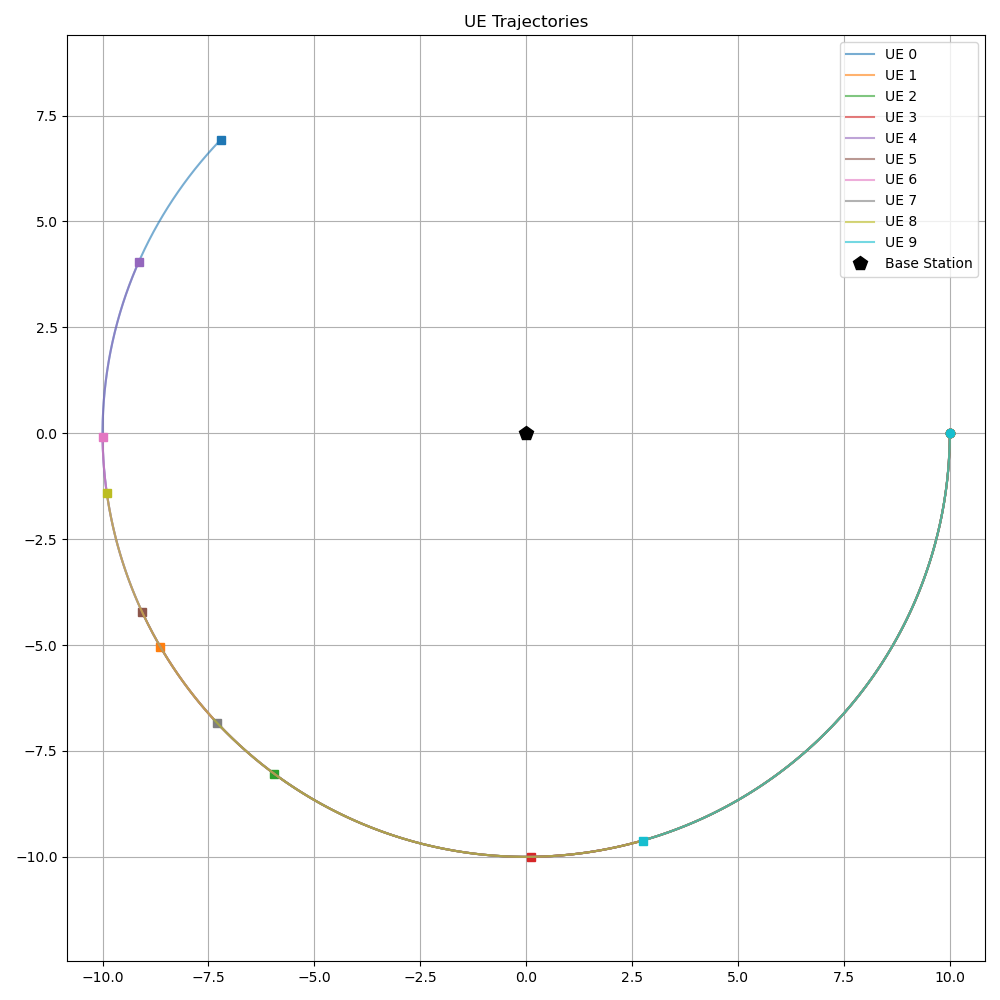
\includegraphics[scale=0.4]{../computos_y_graficas/scheduling_indonesios_mu0_bet/5_7_23_27_55/ue/trajectory.png}}
\end{figure}

\subsubsection{Calidad del canal en el experimento 1}

En primer lugar, podemos prever que las prestaciones de la red están limitadas por el ancho de banda, el ruido y la interferencia.
Según la fórmula de Shannon (suponiendo una SINR de 23 dB ó 200):
$$
C = W \log_2 \left( 1 + \frac {S} {N} \right) [b/s] = \left\lbrace \begin{array}{lr}
100 [MHz] \cdot \log_2 \left( 1 + 200 \right) = 765.11 [Mbps] \quad \mathtt{(UL)} \\
200 [MHz] \cdot \log_2 \left( 1 + 200 \right) = 1.5302 [Gbps] \quad \mathtt{(DL)}
\end{array}
\right.
$$

%{
\includegraphics[scale=0.42]{../comparaciones/scheduling_indonesios_mu0_sin_prioridades/ue/sinr_dl_3d_hist_all_ue_multi.png_cropped.png}}

%{
\includegraphics[scale=0.42]{../comparaciones/scheduling_indonesios_mu0_sin_prioridades/ue/rsrp_dl_3d_hist_all_ue_multi.png_cropped.png}}

\begin{figure}[H]
	\ffigbox[\FBwidth] {
	\caption[Planificación de paquetes - Cuarto caso - Canal (I)]{Distribución del indicador CQI para la dirección DL.
	Las métricas por orden con el número de simulaciones entre paréntesis: FIFO (5), BET (5), EDF (5), LWDF (5), MT (5), RR (5), PF (5).}
	}
	{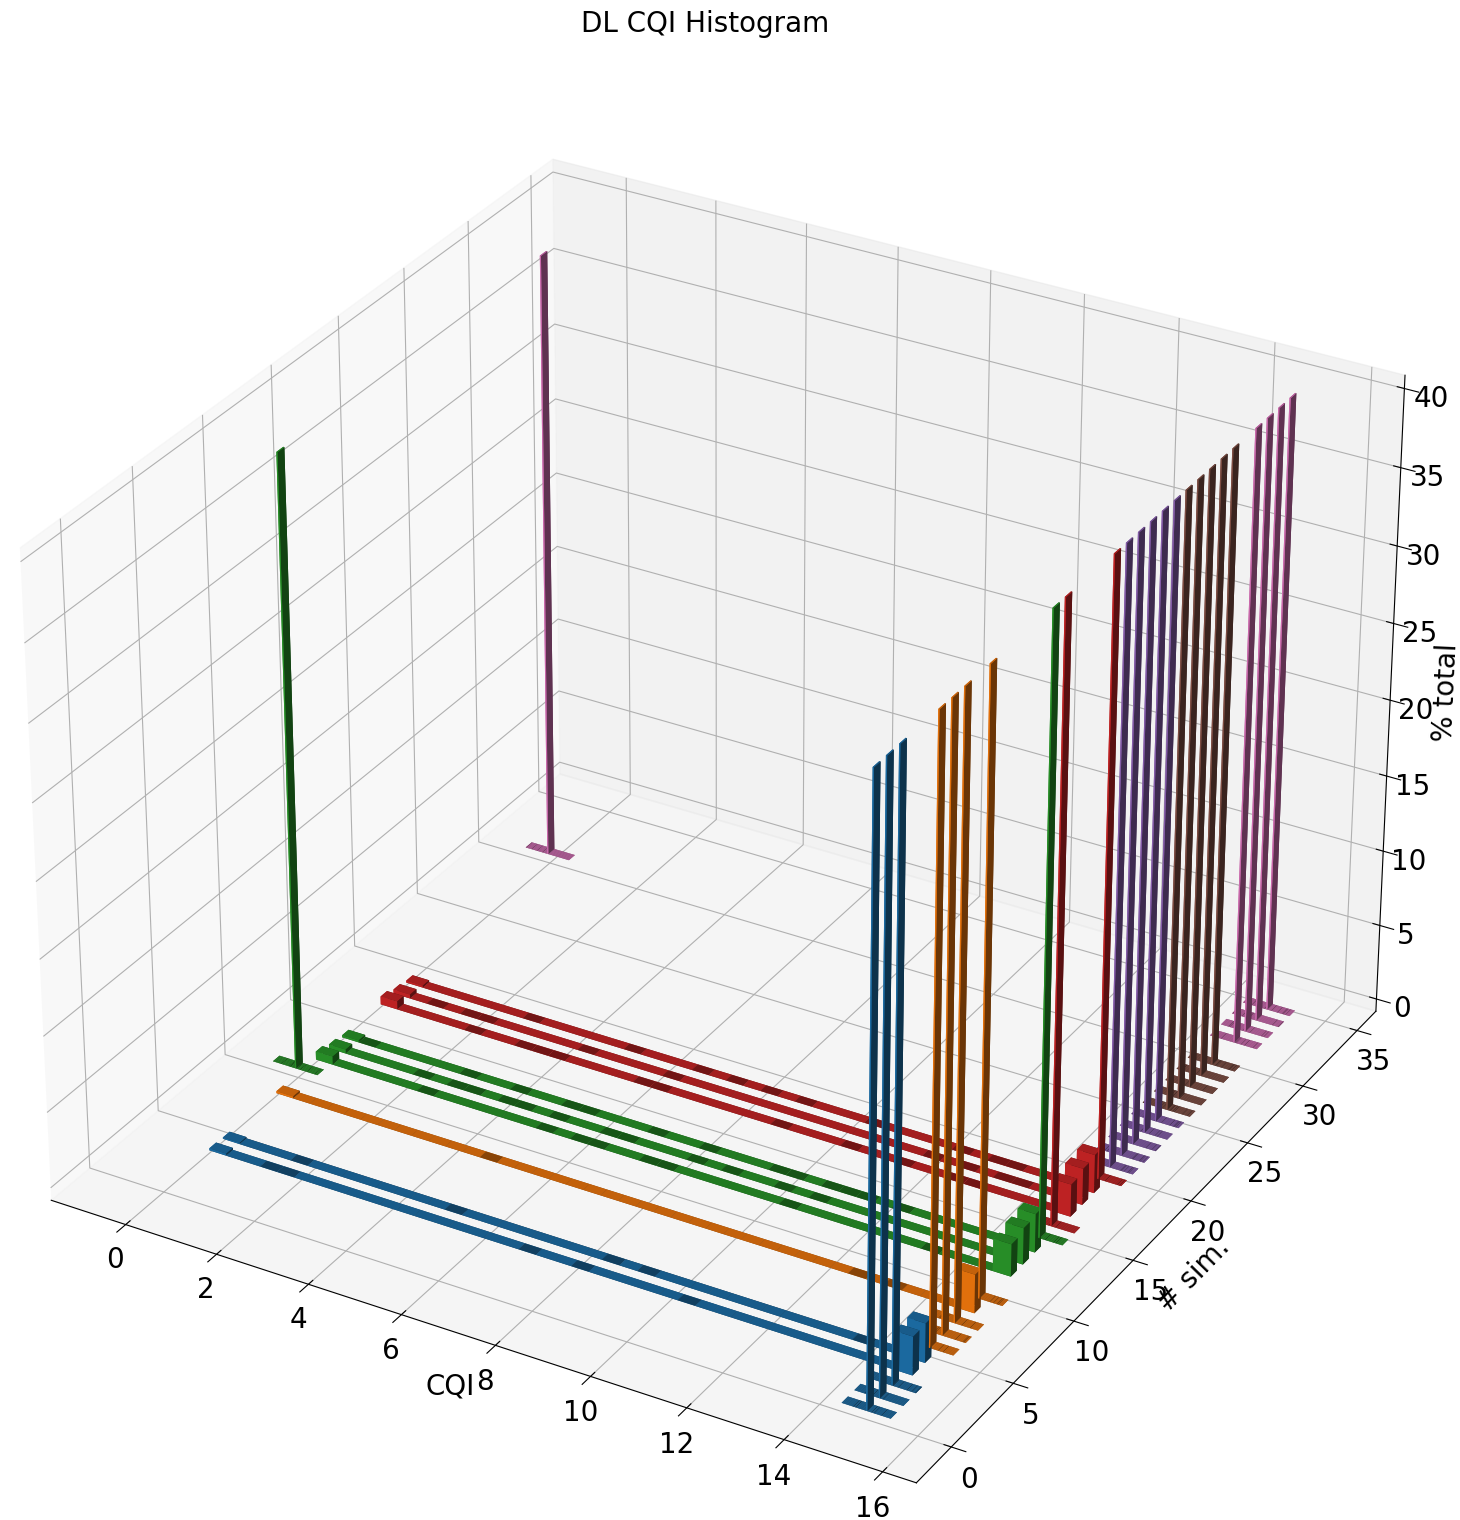
\includegraphics[scale=0.42]{../comparaciones/scheduling_indonesios_mu0_sin_prioridades/ue/cqi_dl_3d_hist_all_ue_multi.png_cropped.png}}
\end{figure}

Si atendemos a los valores indicativos del estado del canal de transmisión (SINR, RSRP, CQI), que se ven en la figura 4.32,
podemos ver que éstos muestran un comportamiento poco diferente al visto anteriormente, cambiando entre métricas.
El motivo es que en el escenario de celda urbana los UE no se desplazan, por lo que no hay variedad de canal a lo largo del tiempo;
habiendo pocos UE, el estado del canal promedio queda determinado por la posición inicial de éstos y los valores de CQI serán los mismos.

\begin{figure}[H]
	\ffigbox[\FBwidth] {
	\caption[Planificación de paquetes - Cuarto caso - MCS (I)]{Distribución del índice MCS para la dirección DL.
	Las métricas por orden con el número de simulaciones entre paréntesis: FIFO (5), BET (5), EDF (5), LWDF (5), MT (5), RR (5), PF (5).}
	}
	{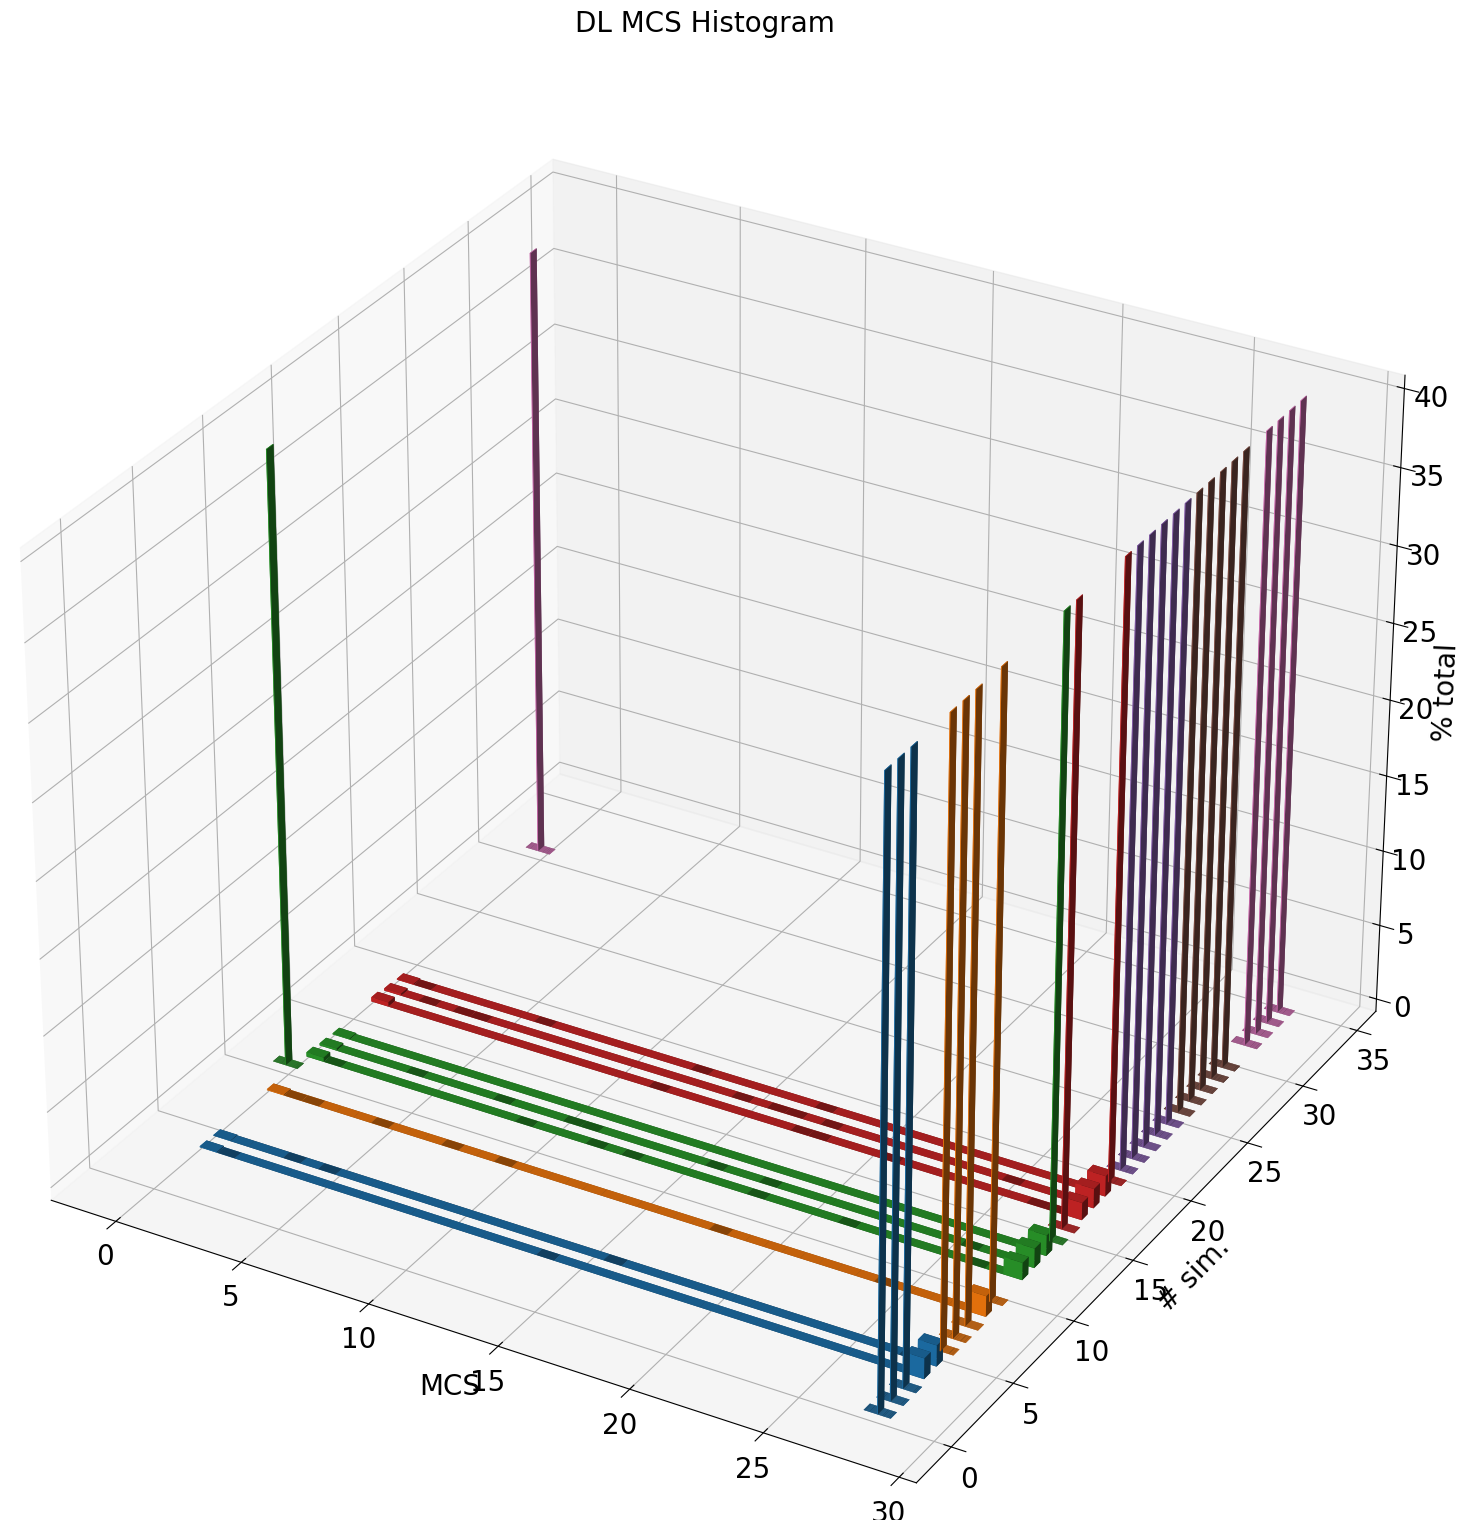
\includegraphics[scale=0.42]{../comparaciones/scheduling_indonesios_mu0_sin_prioridades/ue/mcs_dl_3d_hist_all_ue_multi.png_cropped.png}}
\end{figure}

En la figura 4.33 podemos ver que,
de manera paralela, el índice MCS cambia entre métricas:
Por el mismo motivo, dado que los valores SINR, CQI, etc. son los que determinan el valor MCS elegido,
observamos una distribución de MCS distinta anormal.

%Si observamos los mismos indicadores en la dirección UL podemos ver que éstos no cambian entre métricas, solo con el número de UE;
%a más UE, peor canal.
%
%{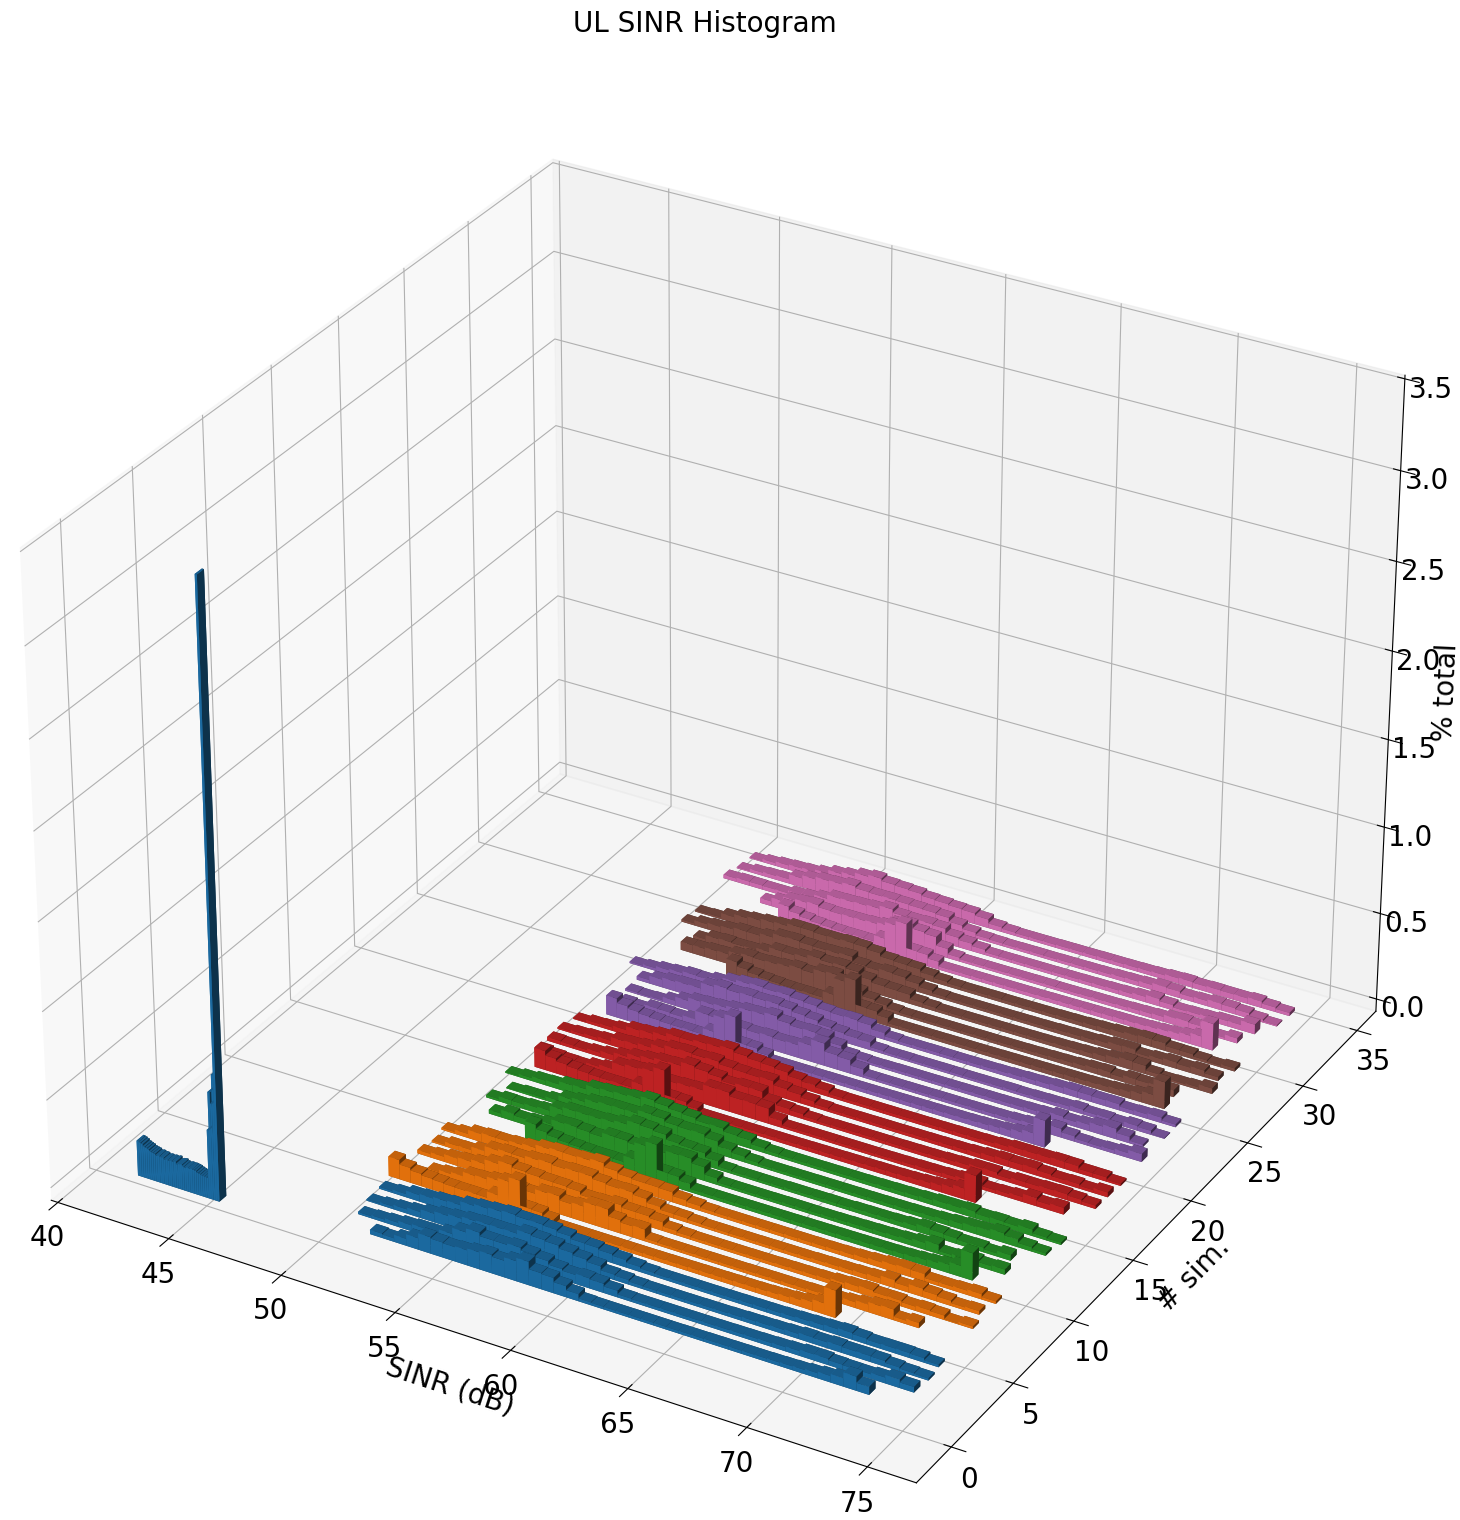
\includegraphics[scale=0.42]{../comparaciones/scheduling_indonesios_mu0_sin_prioridades/ue/sinr_ul_3d_hist_all_ue_multi.png_cropped.png}}
%
%{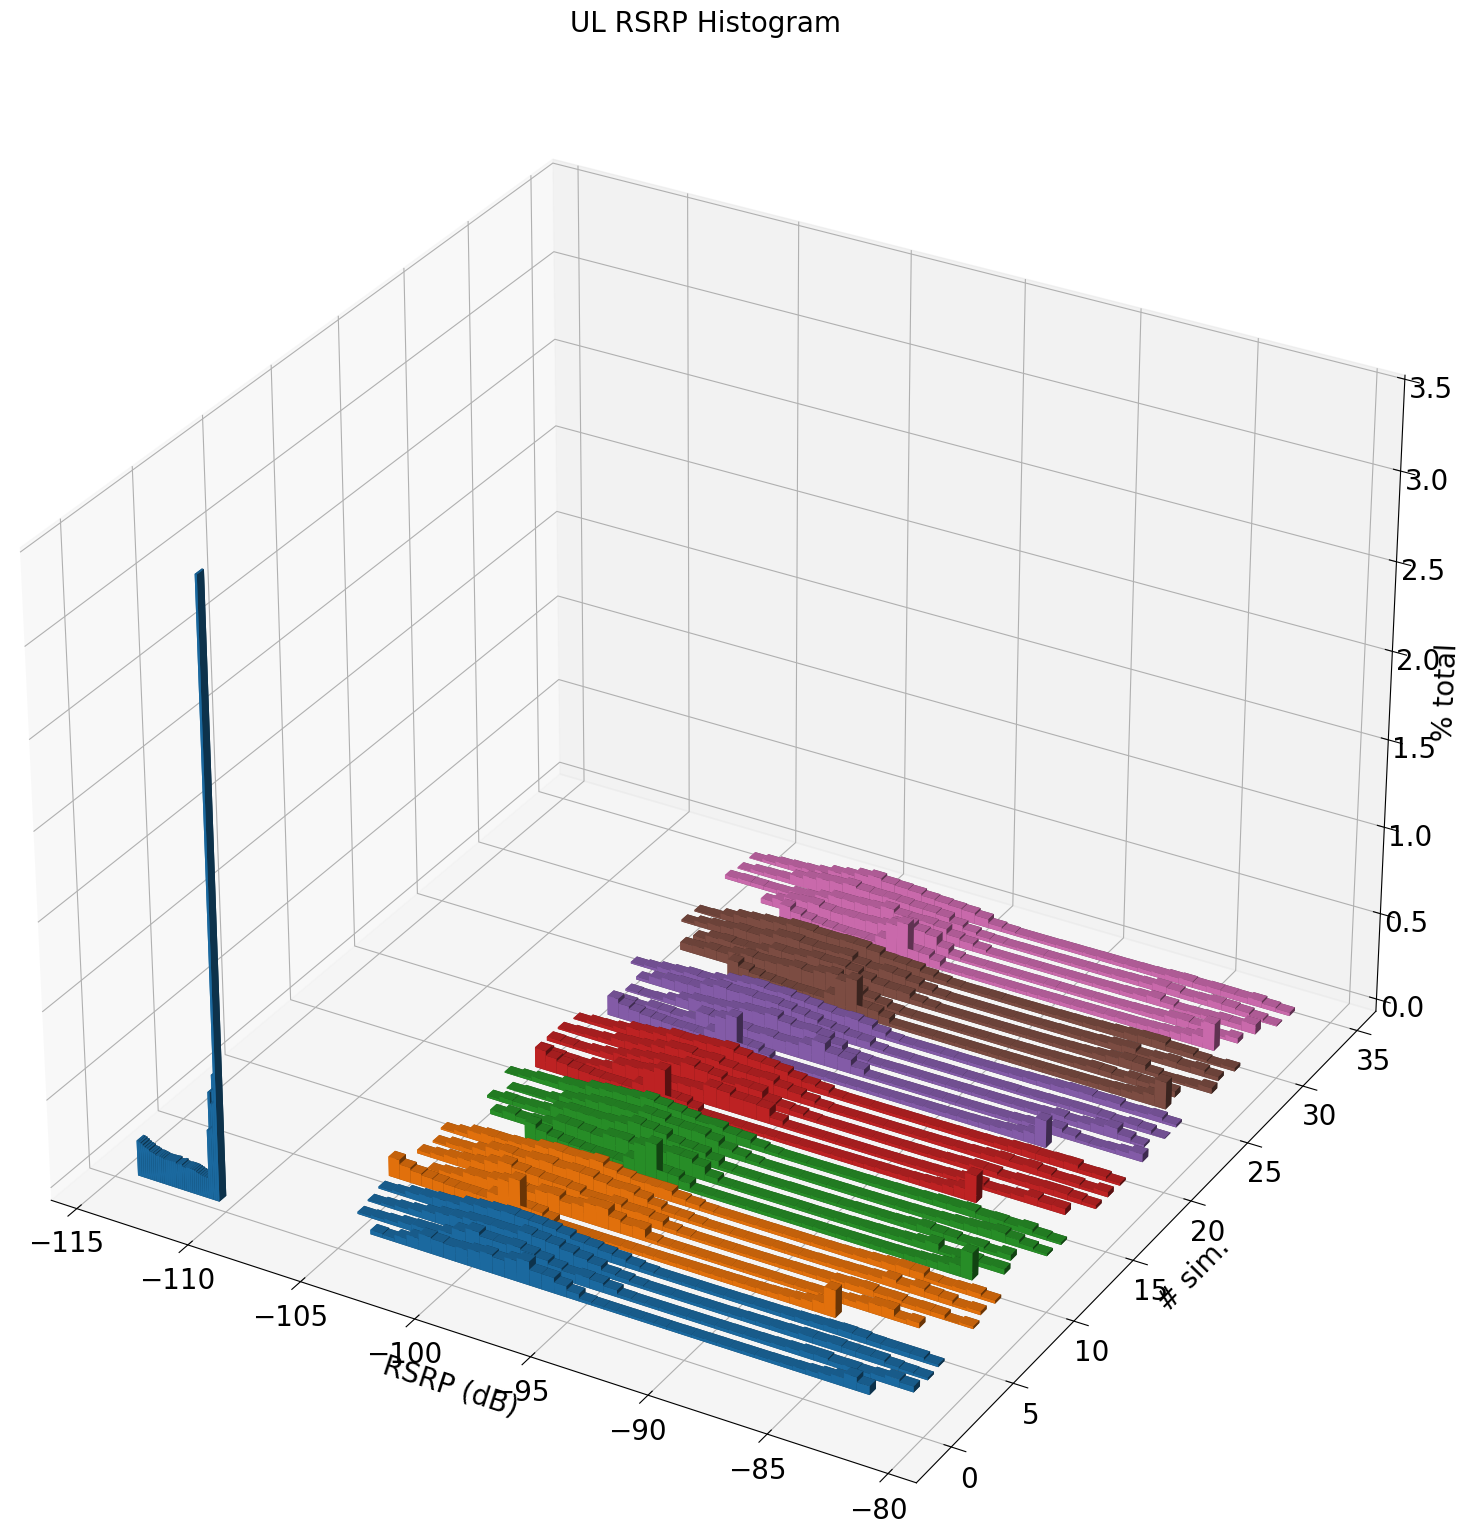
\includegraphics[scale=0.42]{../comparaciones/scheduling_indonesios_mu0_sin_prioridades/ue/rsrp_ul_3d_hist_all_ue_multi.png_cropped.png}}
%
%\begin{figure}[H]
%	\ffigbox[\FBwidth] {
%	\caption[Caso - Packet scheduling - Italianos (canal)]{Distribuciones de los indicadores del estado de canal para la dirección UL.
%	Las métricas por orden con el número de simulaciones entre paréntesis: FIFO (5), BET (5), EDF (5), LWDF (5), MT (5), RR (5), PF (5).
%
%	(Arriba): SINR.
%
%	(Medio): RSRP.
%
%	(Abajo): CQI.}
%	}
%	{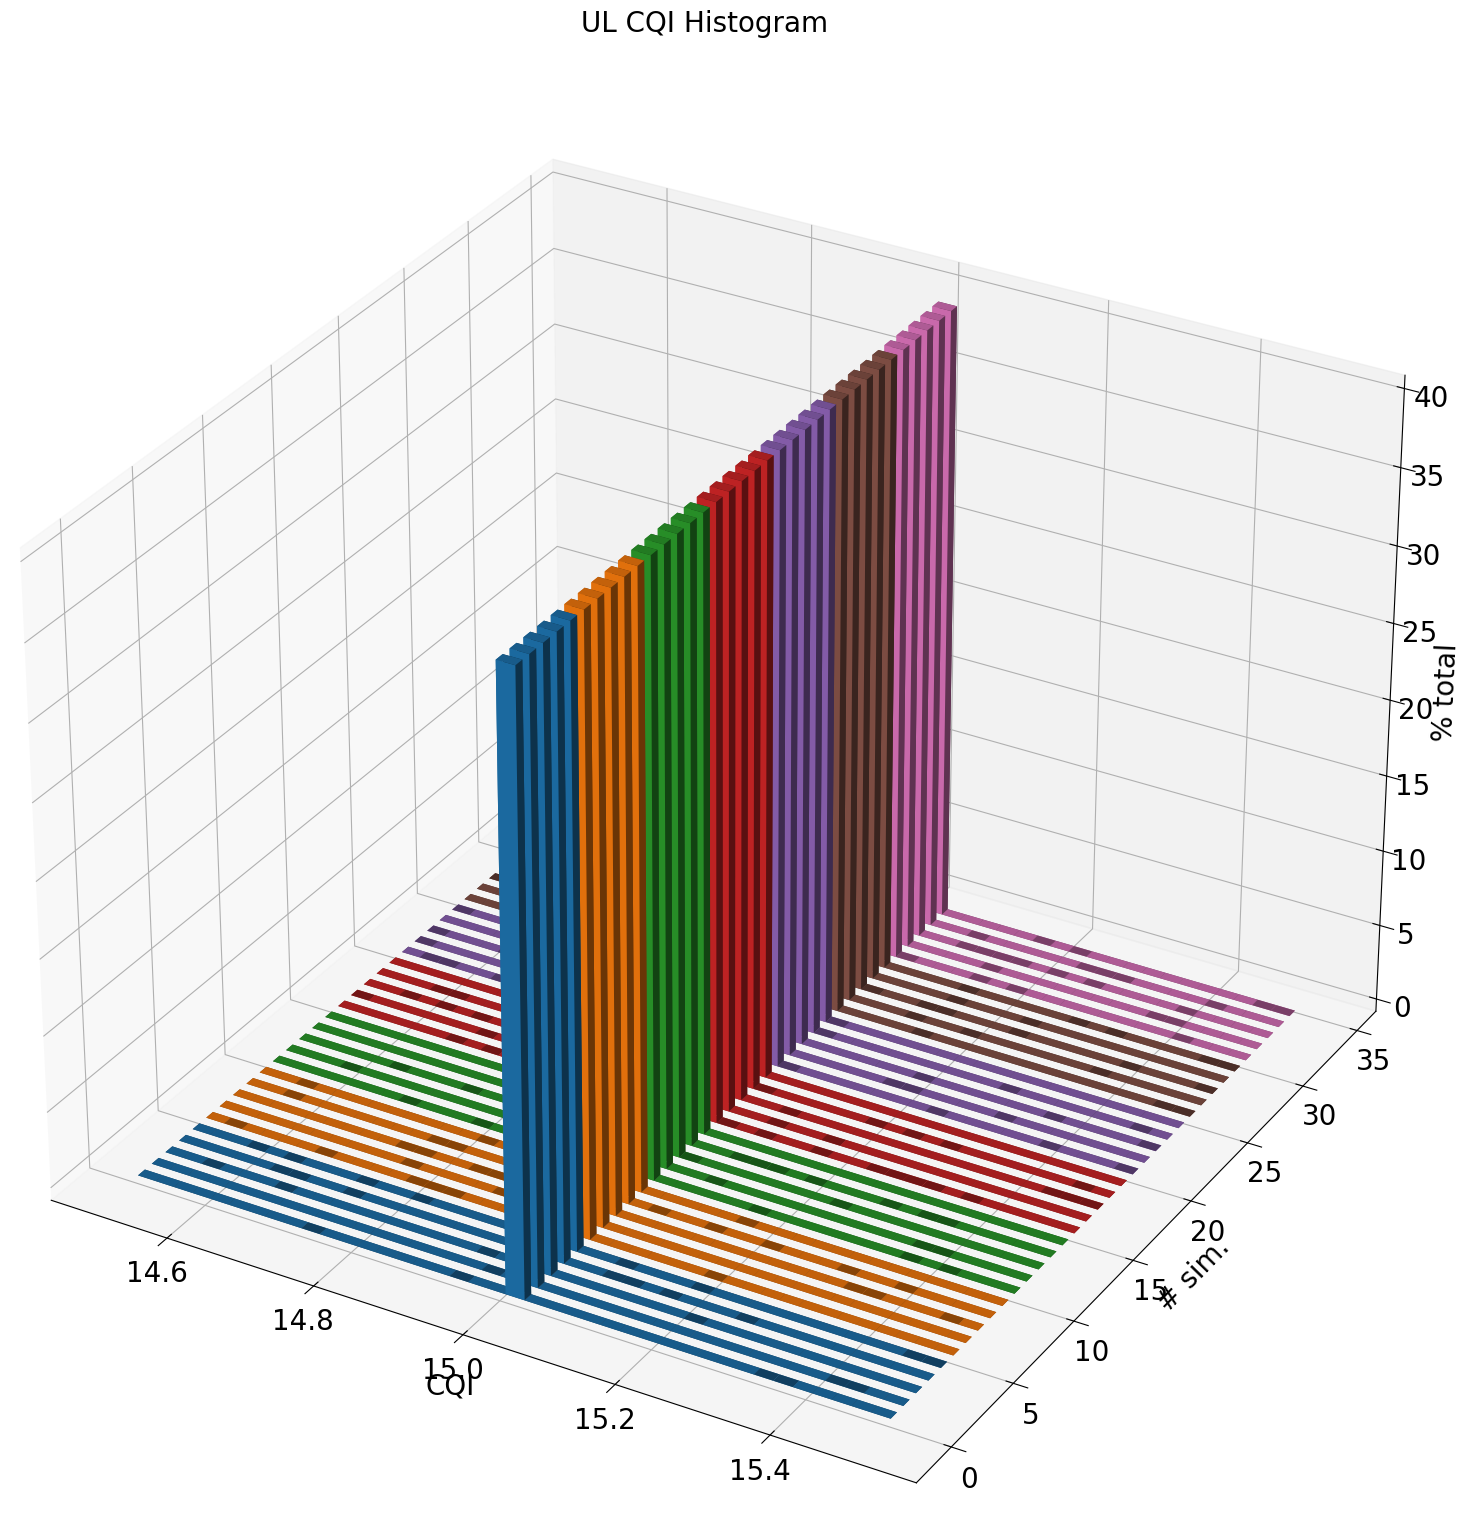
\includegraphics[scale=0.42]{../comparaciones/scheduling_indonesios_mu0_sin_prioridades/ue/cqi_ul_3d_hist_all_ue_multi.png_cropped.png}}
%\end{figure}
%
%Es de esperar, pues el aumento en el número de UE supondrá siempre más interferencia y menos ancho de banda disponible.
%Por otro lado, en la celda urbana sí se aprecian distintas distribuciones de RSRP y SINR entre simulaciones;
%este comportamiento se puede achacar a la lentitud de estos UE, lo que ocasiona que haya poca variedad de canales y los valores se concentren.
%
%De manera paralela, el índice MCS no cambia entre métricas, sólo entre número de UE en la celda. Además, se concentra en 27 en la RMa y en los valores de 0 y 27 en la UMa:
%
%\begin{figure}[H]
%	\ffigbox[\FBwidth] {
%	\caption[Caso - Packet scheduling - Italianos (MCS)]{Distribución del índice MCS para la dirección UL.
%	Las métricas por orden con el número de simulaciones entre paréntesis: FIFO (5), BET (5), EDF (5), LWDF (5), MT (5), RR (5), PF (5).}
%	}
%	{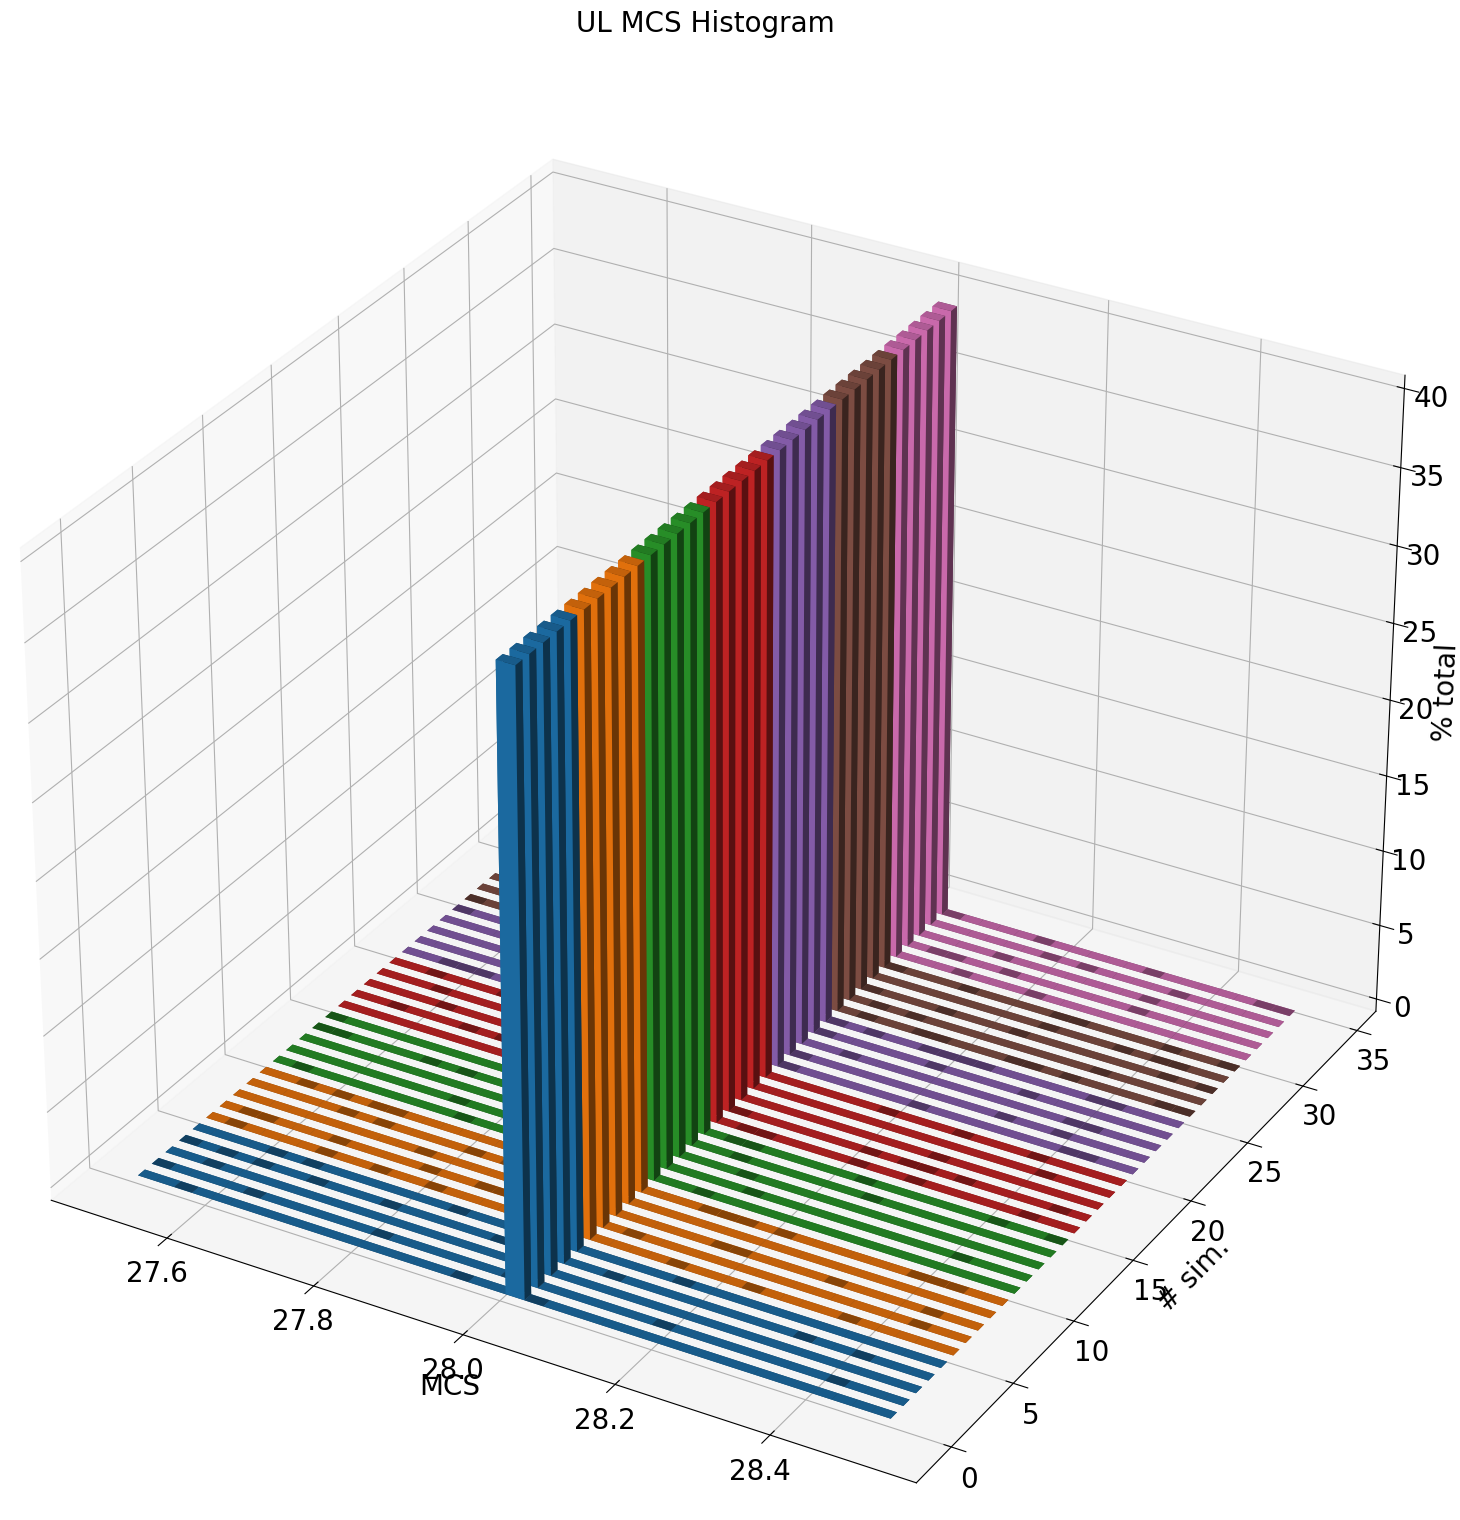
\includegraphics[scale=0.42]{../comparaciones/scheduling_indonesios_mu0_sin_prioridades/ue/mcs_ul_3d_hist_all_ue_multi.png_cropped.png}}
%\end{figure}
%
%Este resultado es, igualmente, esperable, pues los valores SINR, CQI, etc. son los que determinan el valor MCS elegido.
%Además, se trata de una celda pequeña, por lo que estos valores son muy parecidos, lo que ocasiona que se concentren en el valor de 27 en la RMa y en los valores de 0 y 27 en la UMa.

\subsubsection{Prestaciones en el experimento 1}

\begin{center}{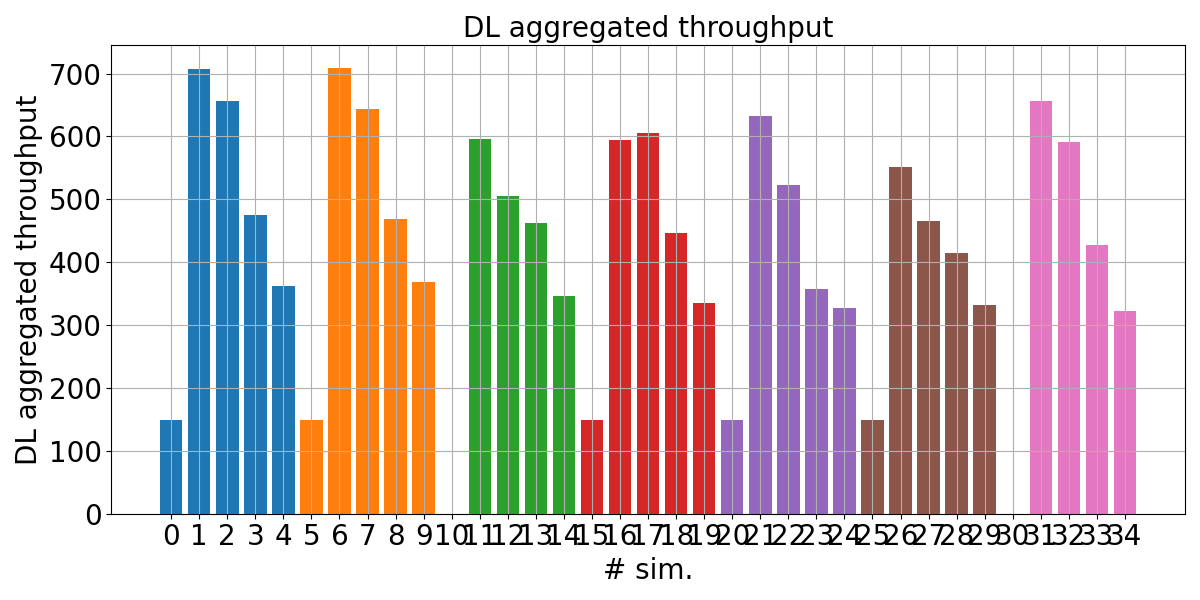
\includegraphics[scale=0.4]{../comparaciones/scheduling_indonesios_mu0_sin_prioridades/ue/dl_agg_throughput_multi_sim.png}}\end{center}

\begin{figure}[H]
	\ffigbox[\FBwidth] {
	\caption[Planificación de paquetes - Cuarto caso - Tasa binaria en la celda (I)]{Tasa binaria de la celda.

	(Arriba): Resultados para la dirección DL.
	Las métricas por orden con el número de simulaciones entre paréntesis: FIFO (5), BET (5), EDF (5), LWDF (5), MT (5), RR (5), PF (5).

	(Abajo): Resultados para la dirección UL.
	Las métricas por orden con el número de simulaciones entre paréntesis: FIFO (5), BET (5), EDF (5), LWDF (5), MT (5), RR (5), PF (5).}
	}
	{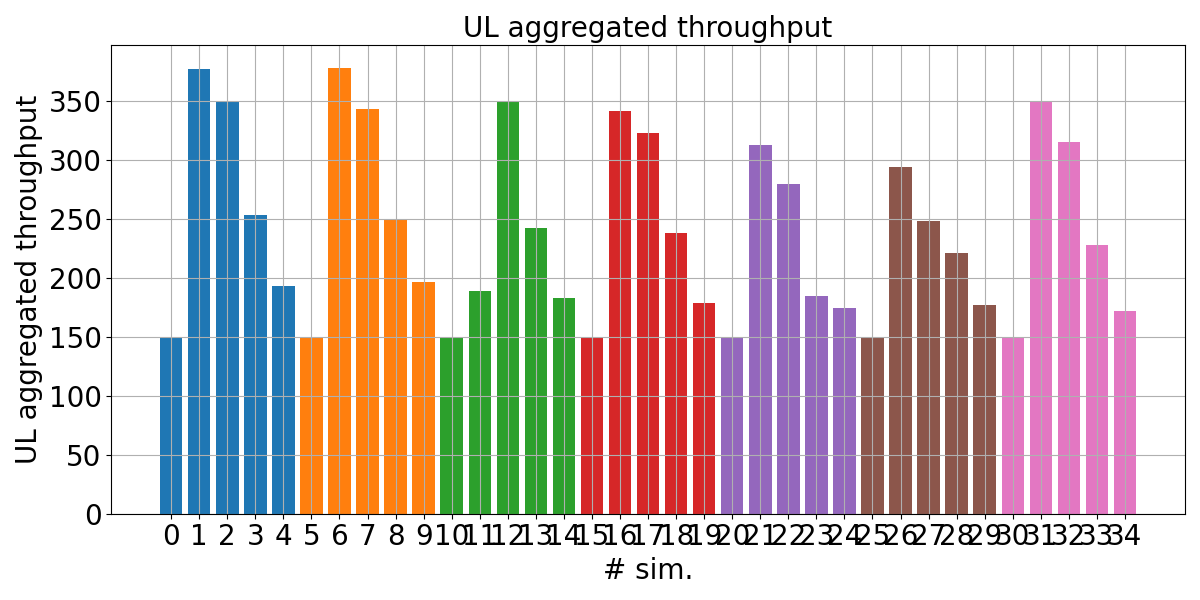
\includegraphics[scale=0.4]{../comparaciones/scheduling_indonesios_mu0_sin_prioridades/ue/ul_agg_throughput_multi_sim.png}}
\end{figure}

El artículo estudia las prestaciones de tasa binaria.
En primer lugar vemos la tasa binaria lograda en la celda en la figura 4.34.
El resultado es, a primera vista, anormal, pues la tasa de la celda deja de aumentar a partir de 5 UE, reduciéndose con cantidades mayores.
La explicación más razonable para este comportamiento es que, debido al movimiento circular elegido, los UE están muy próximos, lo que crea grandes interferencias y resulta en canales, en general, peores;
la calidad, en general, empeora cuando se añaden usuarios en las condiciones que se han elegido.
Por otro lado, todas las métricas muestran un comportamiento muy similar, lo que puede indicar que el estado del canal predomina a la hora de determinar los resultados.

A partir de aquí, consideramos que el experimento no es válido por haberse configurado escenarios que no permiten estudiar el objeto de estudio designado: la planificación de paquetes.

%A continuación mostramos la comparación con los resultados del artículo, que usa la tasa binaria de un UE en promedio:
%
%{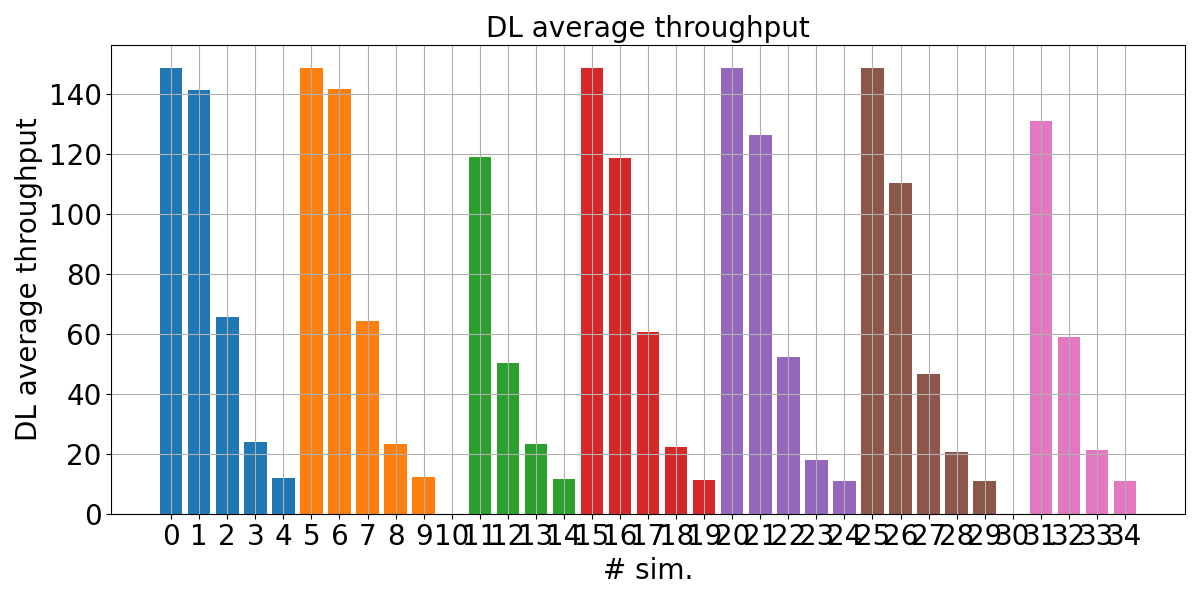
\includegraphics[scale=0.4]{../comparaciones/scheduling_indonesios_mu0_sin_prioridades/ue/dl_ave_throughput_multi_sim.png}}
%
%{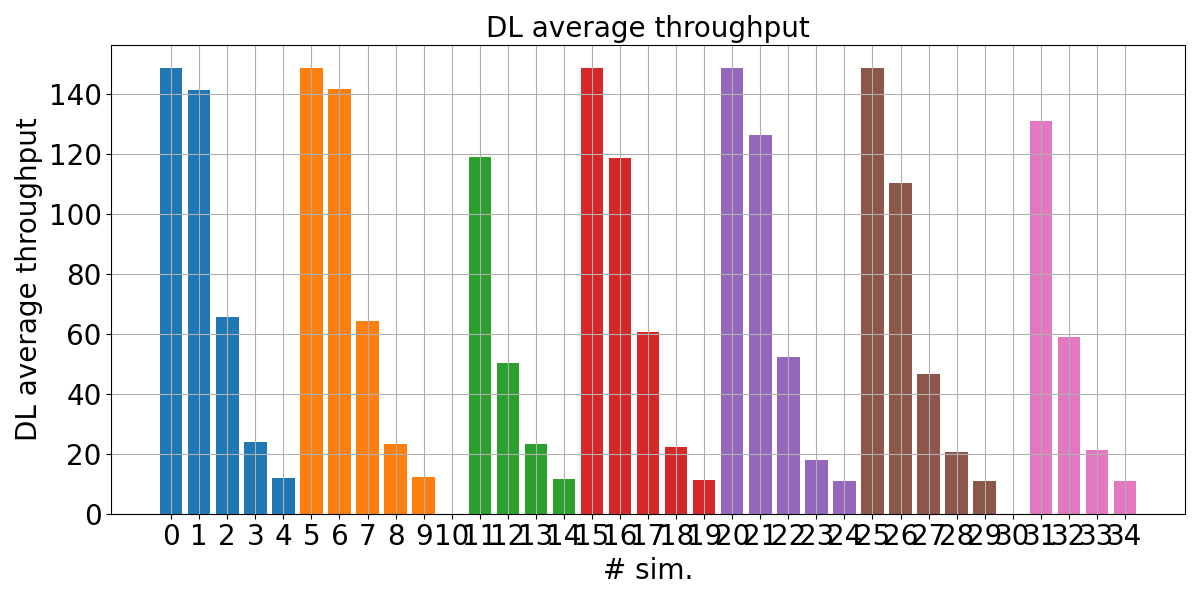
\includegraphics[scale=0.4]{../comparaciones/scheduling_indonesios_mu0_sin_prioridades/ue/dl_ave_throughput_multi_sim.png}}
%
%\begin{figure}[H]
%	\ffigbox[\FBwidth] {
%	\caption[Caso - Packet scheduling - Italianos (\textit{throughput})]{Tasa de un UE en promedio.
%
%	(Arriba): Resultados para la dirección DL.
%	Las métricas por orden con el número de simulaciones entre paréntesis: FIFO (5), BET (5), EDF (5), LWDF (5), MT (5), RR (5), PF (5).
%
%	(En medio): Resultados para la dirección UL.
%	Las métricas por orden con el número de simulaciones entre paréntesis: FIFO (5), BET (5), EDF (5), LWDF (5), MT (5), RR (5), PF (5).
%
%	(Abajo): Resultados de \cite{RefWorks:26}.}
%	}
%	{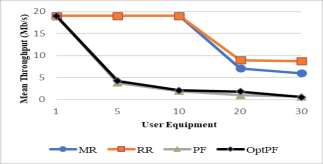
\includegraphics[scale=1.0]{imagenes/scheduling_indonesios/scheduling_indonesios-007.png}}
%\end{figure}

%Por otro lado, se estudia el error en la transmisión:
%
%{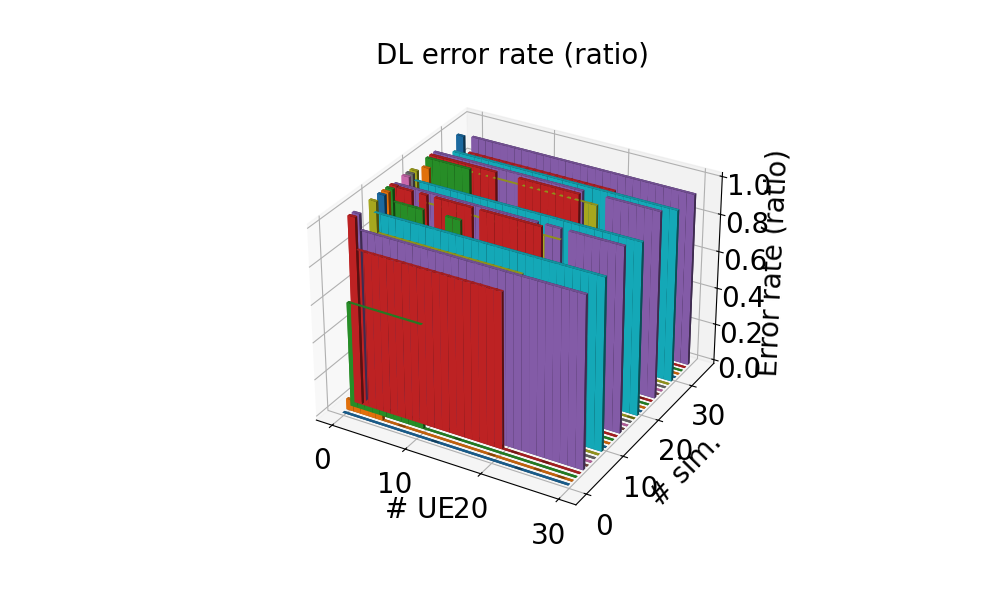
\includegraphics[scale=0.6]{../comparaciones/scheduling_indonesios_mu0_sin_prioridades/ue/dl_er_ratio_3d_multi_sim.png}}
%
%{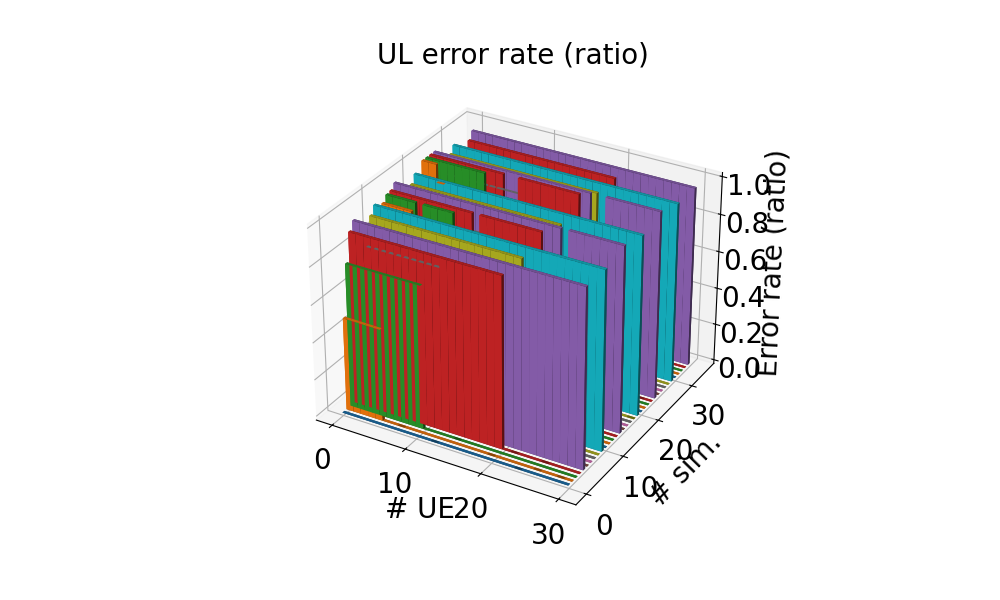
\includegraphics[scale=0.6]{../comparaciones/scheduling_indonesios_mu0_sin_prioridades/ue/ul_er_ratio_3d_multi_sim.png}}
%
%\begin{figure}[H]
%	\ffigbox[\FBwidth] {
%	\caption[Caso - Packet scheduling - Italianos (\textit{throughput})]{Indicadores de error.
%
%	(Arriba): Tasa de error binario por UE y simulación en dirección DL.
%	Las métricas por orden con el número de simulaciones entre paréntesis: FIFO (5), BET (5), EDF (5), LWDF (5), MT (5), RR (5), PF (5).
%
%	(En medio): Tasa de error binario por UE y simulación en dirección UL.
%	Las métricas por orden con el número de simulaciones entre paréntesis: FIFO (5), BET (5), EDF (5), LWDF (5), MT (5), RR (5), PF (5).
%
%	(Abajo): Tasa de paquetes entregados de \cite{RefWorks:26}.}
%	}
%	{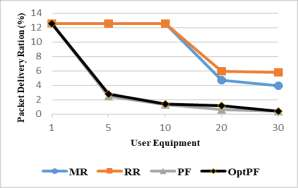
\includegraphics[scale=1.0]{imagenes/scheduling_indonesios/scheduling_indonesios-010.png}}
%\end{figure}

%\subsubsection{Descripción del experimento 2: prioridades}
%
%Ahora, proponemos un experimento con el objeto de estudiar el efecto de asignar una prioridad a los UE con cada una de las métricas.
%Se ha simulado con 10 UE, cada una de las métricas pero con el orden de prioridades alterado:
%prioridades que iban del 1 al 10.
%
%\subsubsection{Calidad del canal en el experimento 2}
%
%En primer lugar, podemos suponer las mismas prestaciones de la red en lo que respecta a capacidad,
%la calidad de los canales de transmisión será la misma que en el anterior experimento, los valores indicativos del estado del canal de transmisión (SINR, RSRP, CQI) serán iguales.
%En este caso, sí será determinante el efecto de las métricas sobre el del canal al contar con el mismo canal en todos los experimentos.
%
%\subsubsection{Prestaciones en el experimento 2}
%
%En primer lugar, si observamos la tasa binaria lograda en la celda, vemos diferentes comportamientos:
%
%\begin{figure}[H]
%	{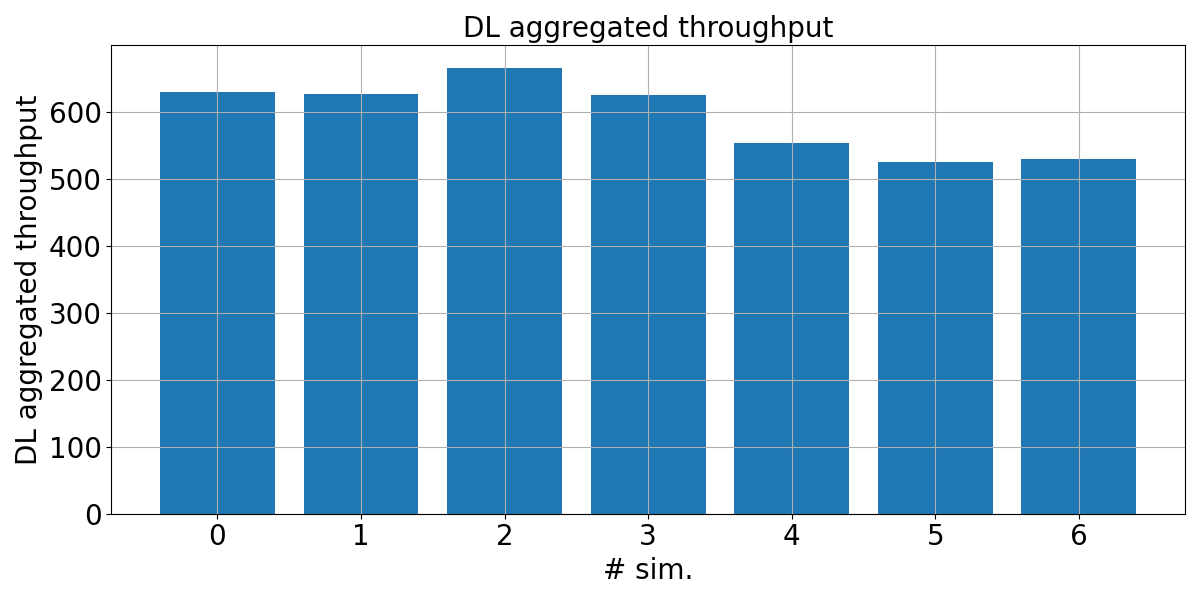
\includegraphics[scale=0.3]{../comparaciones/scheduling_indonesios_mu0_prioridades/ue/dl_agg_throughput_multi_sim.png}}
%	\ffigbox[\FBwidth] {
%	\caption[Caso - Packet scheduling - Italianos (\textit{throughput})]{Tasa binaria de la celda.
%
%	(Arriba): Resultados para la dirección DL.
%	Las métricas por orden: FIFO, BET, EDF, LWDF, MT, RR, PF.
%
%	(Abajo): Resultados para la dirección UL.
%	Las métricas por orden: FIFO, BET, EDF, LWDF, MT, RR, PF.}
%	}
%	{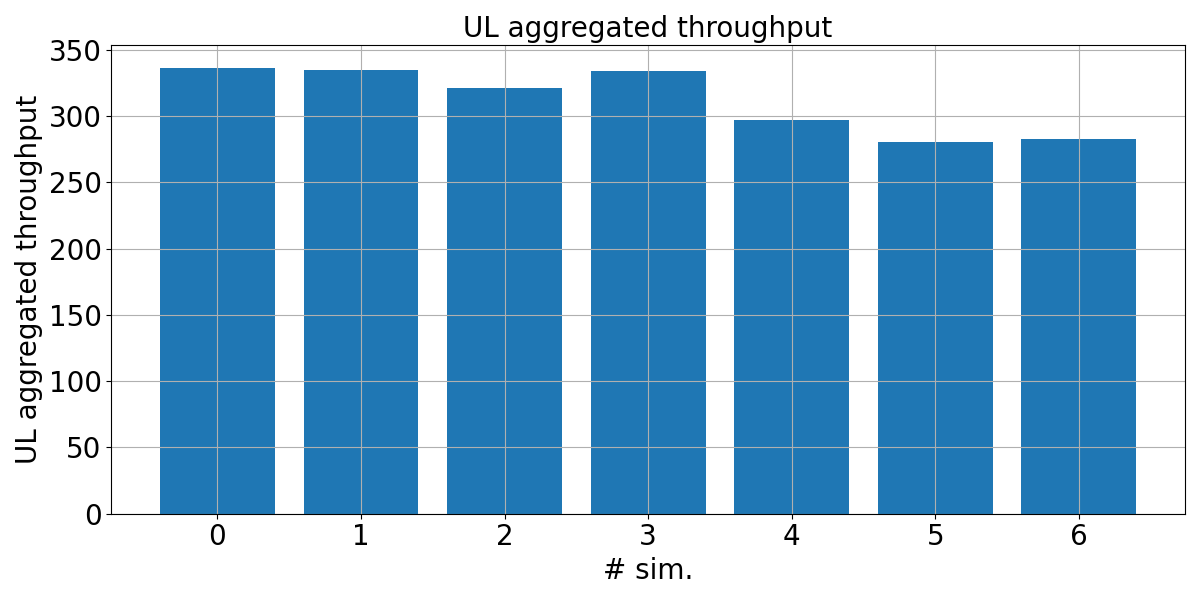
\includegraphics[scale=0.3]{../comparaciones/scheduling_indonesios_mu0_prioridades/ue/ul_agg_throughput_multi_sim.png}}
%\end{figure}

%\subsection{Australianos}
%
%No se ha simulado.
%
%Viene de \cite{RefWorks:68}
%
%Describe una metodología para emular LTE mediante computadora.
%
%Contiene una simulación de métricas en LTE usando la metodología.

\chapter{Caso de uso: comunicaciones celulares en entornos vehiculares (C-V2X)}

\section{Introducción}

Las comunicaciones vehiculares son un caso de uso desde generaciones de comunicaciones móviles más antiguas.
Antes de 5G, las tecnologías de redes móviles de 3GPP ya cubrían casos de uso relacionados con vehículos que no requerían gran fiabilidad ni latencias mínimas,
como el manejo de flotas o la monitorización de vehículos.
Los estándares de LTE ya tenían en cuenta el caso de uso de los vehículos, introduciendo el concepto de comunicaciones celulares vehiculares (\textit{Cellular Vehicle to Everything}, C-V2X),
es decir, las comunicaciones de vehículos mediante sistemas celulares, para diferenciarlo de las comunicaciones que se llevan a cabo con otras tecnologías.
LTE también introdujo nuevas específicas para C-V2X, como el enlace lateral (\textit{sidelink}), también llamado PC5,
que consistía en la conexión directa de dos vehículos.
Por su parte, la NR de 5G promete mejorar los requerimientos de calidad de servicio y ofrecer latencias a partir de 10 ms y tasas binarias por encima de 100 Mbps,
prestaciones muy atractivas para las aplicaciones con vehículos.
Se consideran de interés las aplicaciones sensibles a la latencia y se ha puesto el foco en hacer realizable el paradigma de la movilidad conectada, cooperativa y automatizada (Connected, Cooperative and Automated Mobility, CCAM),
una serie de usos más exigentes en lo que respecta a prestaciones, que se cree que permitiría explotar nuevos servicios.
\cite{RefWorks:25}

El problema de las comunicaciones es muy complejo, por lo que uno de los aspectos de su desarrollo que se han señalado es la evaluación de despliegues.
Este problema contempla las dificultades de los traspasos entre celdas (\textit{handover}) y redes de distintos operadores (\textit{roaming}),
la limitación en la cobertura de 5G,
la provisión de servicios en unos y otros operadores o la regulación de cada lugar.
\cite{RefWorks:25}
Una propuesta atrevida se da en \cite{RefWorks:25}, que ofrece un marco y una metodología que puede implementarse con varias herramientas disponibles para el desarrollador.

Por otro lado, está la investigación de cada uno de los problemas particulares de C-V2X,
que progresa de manera independiente, en función de las iniciativas de investigación que haya.
La iniciativa a nivel europeo de \textit{5GPPP} \cite{RefWorks:101} ha reunido varios proyectos que han tenido como objetivo resolver algunos de estos problemas y han dejado una producción interesante \cite{RefWorks:102, RefWorks:103},
como \textit{5G-MOBIX} \cite{RefWorks:107}, \textit{5G-CARMEN} \cite{RefWorks:106}, \textit{5GCroCo} \cite{RefWorks:105}, \textit{5GCAR} \cite{RefWorks:104}.

La comunicación directa entre vehículos (V2V) no puede ser representada en el emulador, por lo que las tecnologías ideadas para este problema, como PC5, no se estudian.
Sí se han considerado varios experimentos en función de propuestas que hay en la academia.
Por orden, diferenciamos los experimentos de C-V2X con despliegues reales \cite{RefWorks:25, RefWorks:49},
las simulaciones que se llevaron a cabo con otros simuladores disponibles \cite{RefWorks:50, RefWorks:51}
y las simulaciones que se llevaron a cabo con otras metodologías \cite{RefWorks:48, RefWorks:52}.

\section{Servicios de C-V2X en traspasos (\textit{5G-MOBIX})}

\subsubsection{Introducción}

El artículo \cite{RefWorks:25} forma parte de la producción literaria del proyecto \textit{5G-MOBIX}.
\cite{RefWorks:107}
Se trata de un proyecto a nivel europeo, que engloba a varias empresas e instituciones de investigación,
que estudia la conducción autónoma y se enfoca en el problema del traspaso entre redes de distintos operadores o de distintas regiones.
El proyecto remarca la importancia de la red móvil en la implementación de la conducción autónoma;
desarrolla una metodología novedosas para evaluar los despliegues de 5G y su configuración de cara a ofrecer servicios para la condición autónoma.
Más importante para nuestro caso es que en el proyecto se realizan y documentan experimentos en una red de 5G que pueden recrearse con \textit{FikoRE} para comparar los resultados y obtener nuevas concusiones.

Se ha representado el experimento con \textit{FikoRE}
(véase \textit{Caso de uso (III): C-V2X (5GMOBIX)} en el anexo \textit{Simulaciones (metadatos)}).

\subsubsection{Descripción del experimento}

El experimento original era un adelantamiento de vehículos que tenía lugar al mismo tiempo que un traspaso entre operadoras en la frontera hispano-portuguesa.
Un vehículo autónomo adelanta a otro valíendose de los mensajes CAM (tipo de información usada en conducción autónoma) intercambiados con otros vehículos mediante la red móvil.
Los parámetros del experimento se resumen en la figura 5.1.

\begin{figure}[H]
	\ffigbox[\FBwidth] {
	\caption[C-V2X - Primer caso - Características del experimento propuesto]{
	Experimento descrito en \cite{RefWorks:25}:
\begin{itemize}
\item \textbf{Escenario:}
Las entidades gNodeB se encuentran en Tuy (España) y Valença (Portugal), fueron desplegadas por Nokia España y Nokia Portugal y pertenecen a los operadores Telefónica y NOS, respectivamente.
Es un despliegue NSA.
El servidor MQTT se ejecuta en un servidor MEC perteneciente a Telefónica y ubicado en la misma carreterera.
Se usan SIM de Telefónica.
\item \textbf{Usuarios:} dos Citroen C4 Picasso (ES-PT\_UE\_01, ES-PT\_UE\_02) y un Volkswagen Golf (ES-PT\_UE\_03).
Uno de los Citroen y el Volkswagen cuentan con una autonomía de \textit{Nivel 4} (control longitudinal y lateral), mientras que el otro Citroen únicamente está conectado a la red.
\item \textbf{Terminales (OBU):} HMCU (Hybrid Modular Communication Unit) CTAG.
Incorpora un receptor Trimble BD920 GPS, un módem Quectel 5G RM500Q-GL y una antena Poynting PUCK-2.
\item \textbf{Servicio de red:}
Los vehículos intercambian mensajes mediante un servidor MQTT (Message Queuing Telemetry Transport).
Los mensajes enviados por ES-PT\_UE\_01 y ES-PT\_UE\_02 al MEC (UL) se agregan y reconducen a ES-PT\_UE\_03 (DL).
Se emplea TCP.
ES-PT\_UE\_01 y ES-PT\_UE\_02 envían mensajes a una tasa de 10 Hz;
ES-PT\_UE\_03 reciben mensajes a una tasa de 20 Hz.
\item \textbf{Servicio implementado:}
La información CAM se combina con datos de los sensores del vehículo (cámara y LiDAR), estos son los parámetros de entrada del algoritmo de control del vehículo.
De esta manera, el vehículo que adelanta (ES-PT\_UE\_03) recibe la posición y la velocidad del resto de vehículos y decide cómo proceder.
\item \textbf{Pruebas:}
Se llevan a cabo seis pruebas de 60 segundos cada una.
\end{itemize}
	}
	}
	{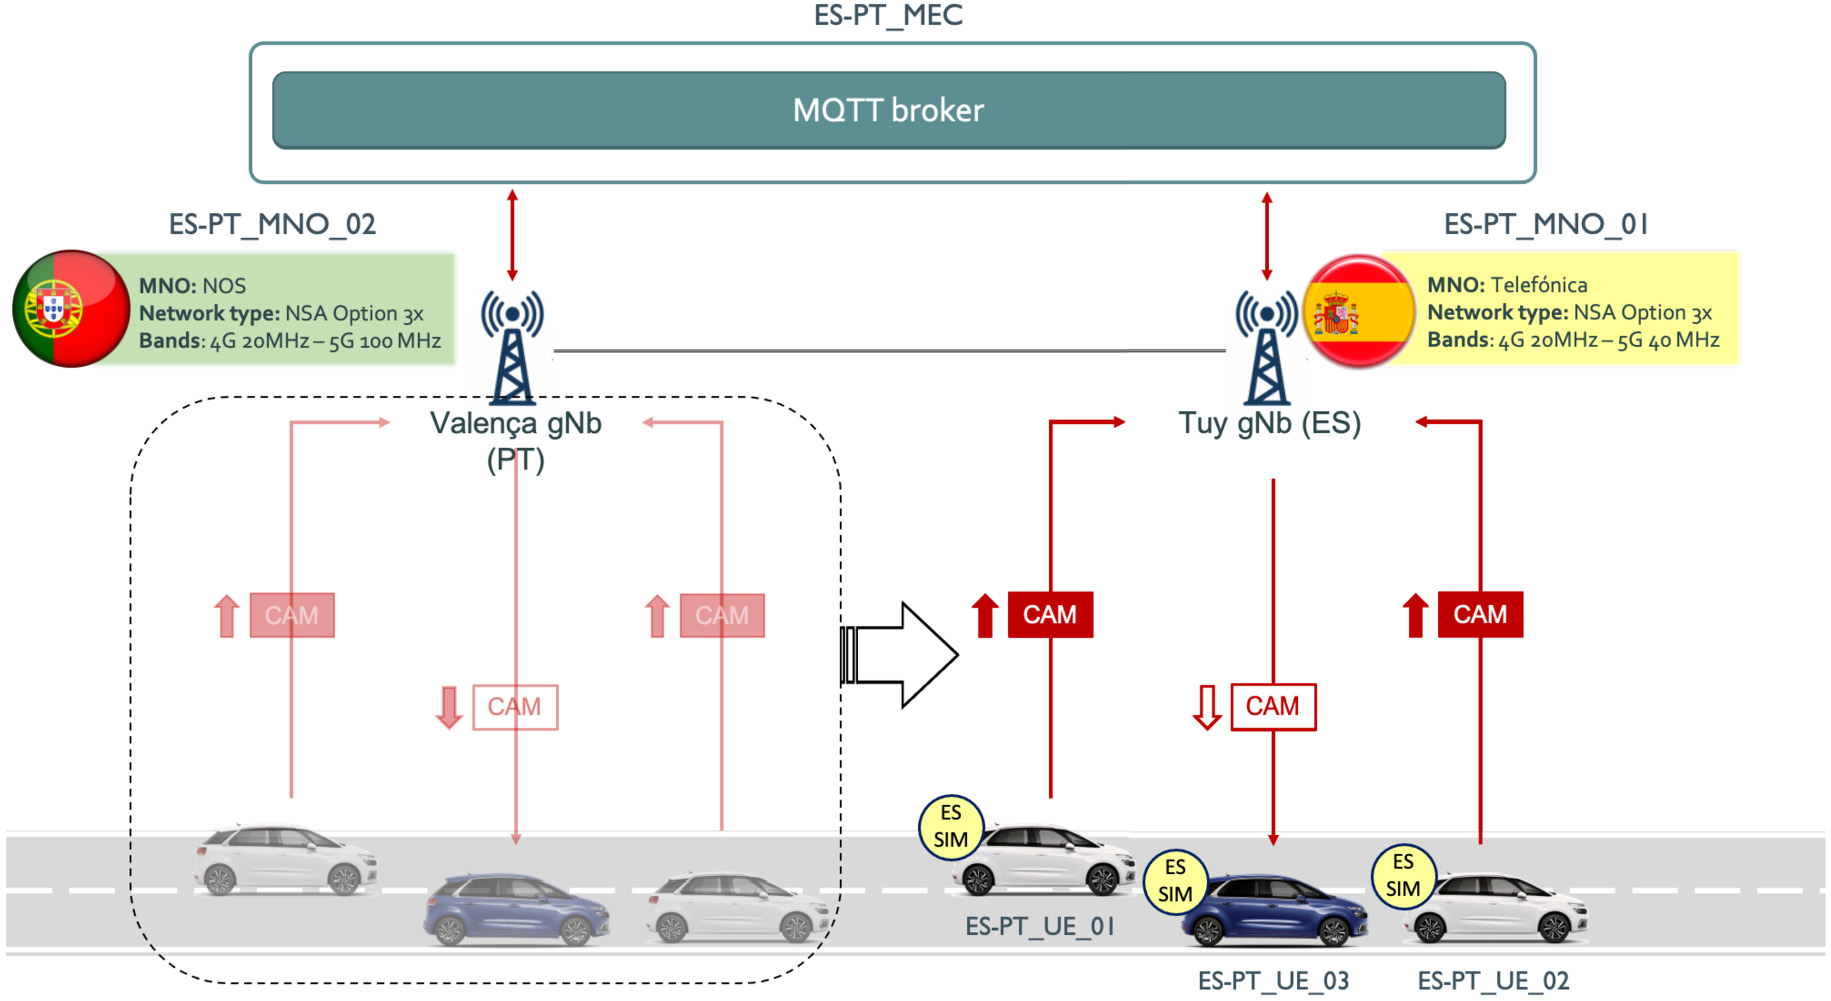
\includegraphics[scale=0.25]{imagenes/v2x_5gmobix/v2x_5gmobix-005.png}}
\end{figure}

Se ha adaptado el mismo experimento para realizarse con el emulador \textit{FikoRE}:

\begin{itemize}
\item Al no moder representarse varias celdas para representar un traspaso, se re representa una para simular la desconexión el terminal.
\item Se han representado tres UE que se alejan en línea recta de la gNB, de la misma manera que en el experimento.
\item Para el tráfico, se ha elegido un tráfico de 0.1 Mbps en dos UE (los que informan) y 0.2 Mbps en el otro (el que adelanta).
\item Se ha representado el experimento en una celda rural (RMa)
\item Se ha simulado el mismo experimento con distintas velocidades para ver el efecto de éstas en la transmisión.
Las velocidades van de 10 km/h a 120 km/h.
\item El mismo experimento se ha llevado a cabo con todas las numerologías para estudiar el efecto de las distintas configuraciones.
\end{itemize}

\begin{center}{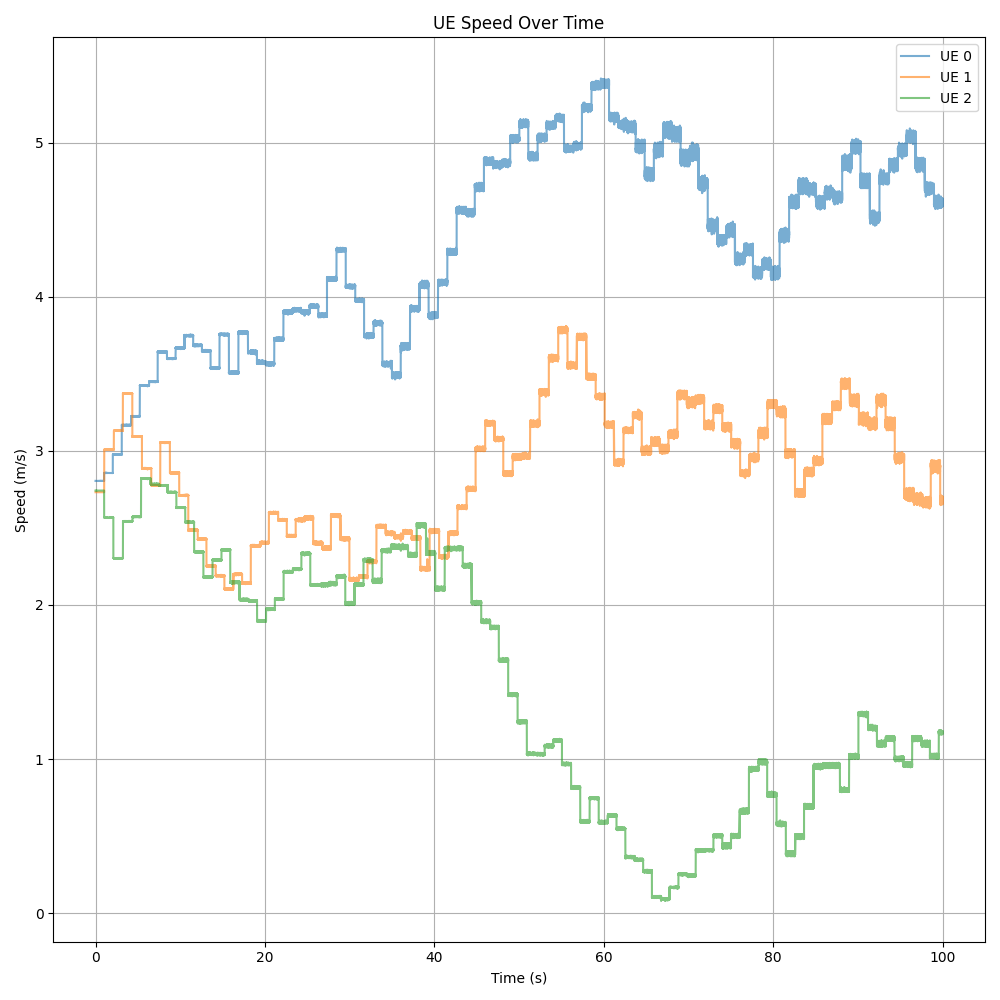
\includegraphics[scale=0.50]{../computos_y_graficas/v2x_5gmobix_num_0/5_9_11_19_47/ue/speed.png}}\end{center}

\begin{center}{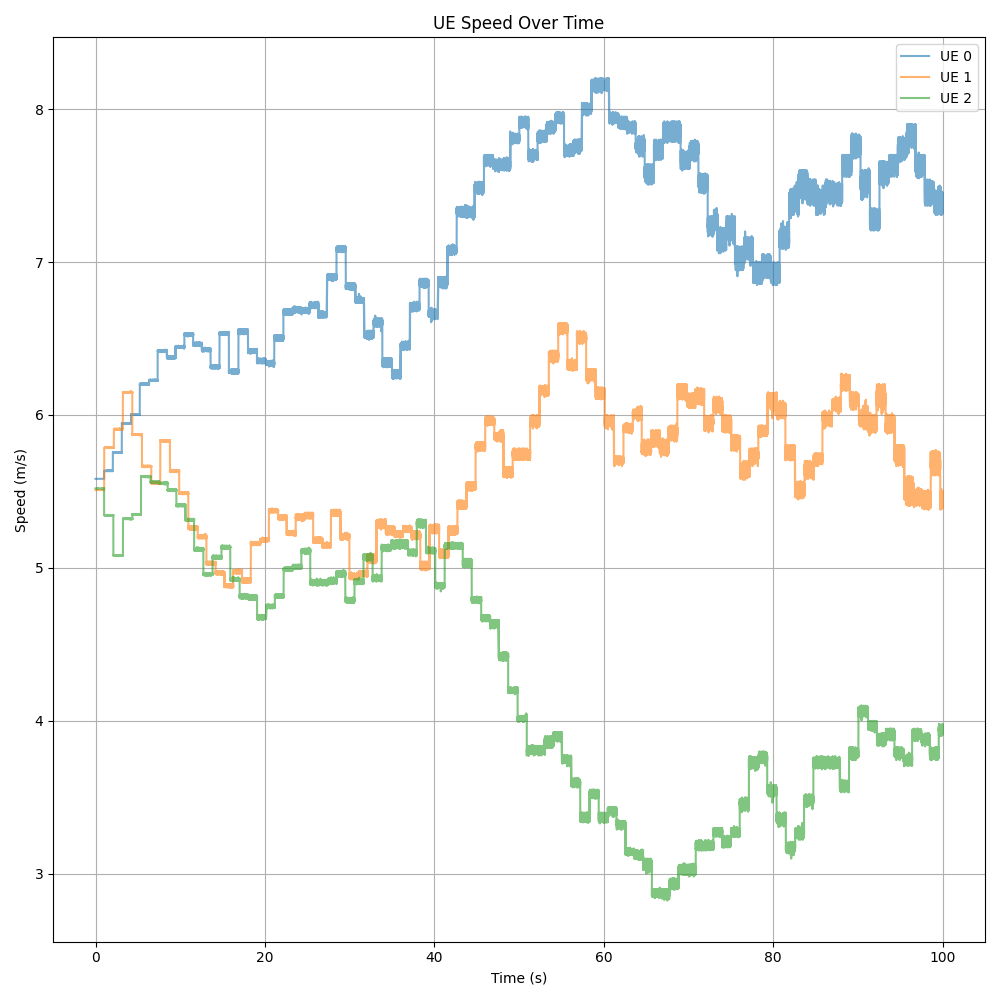
\includegraphics[scale=0.50]{../computos_y_graficas/v2x_5gmobix_num_0/5_9_11_28_46/ue/speed.png}}\end{center}

\begin{center}{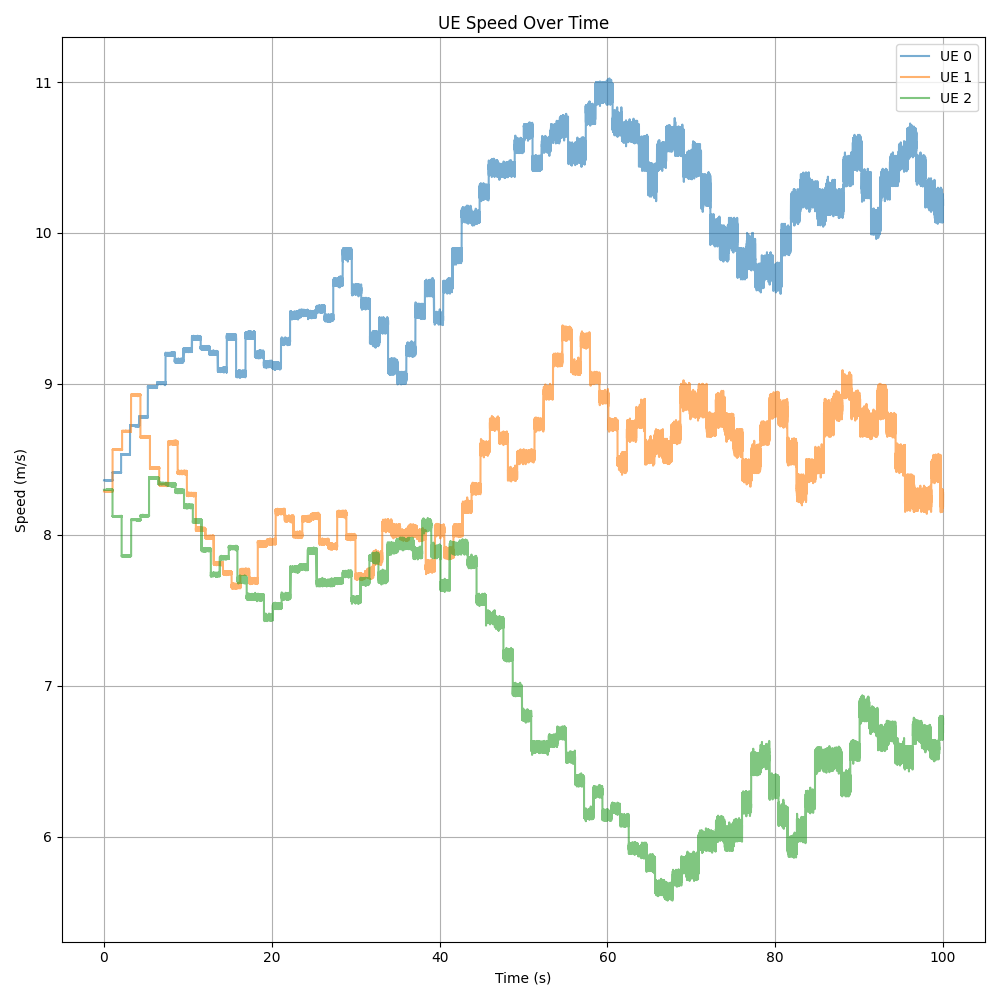
\includegraphics[scale=0.50]{../computos_y_graficas/v2x_5gmobix_num_0/5_9_11_30_26/ue/speed.png}}\end{center}

\begin{center}{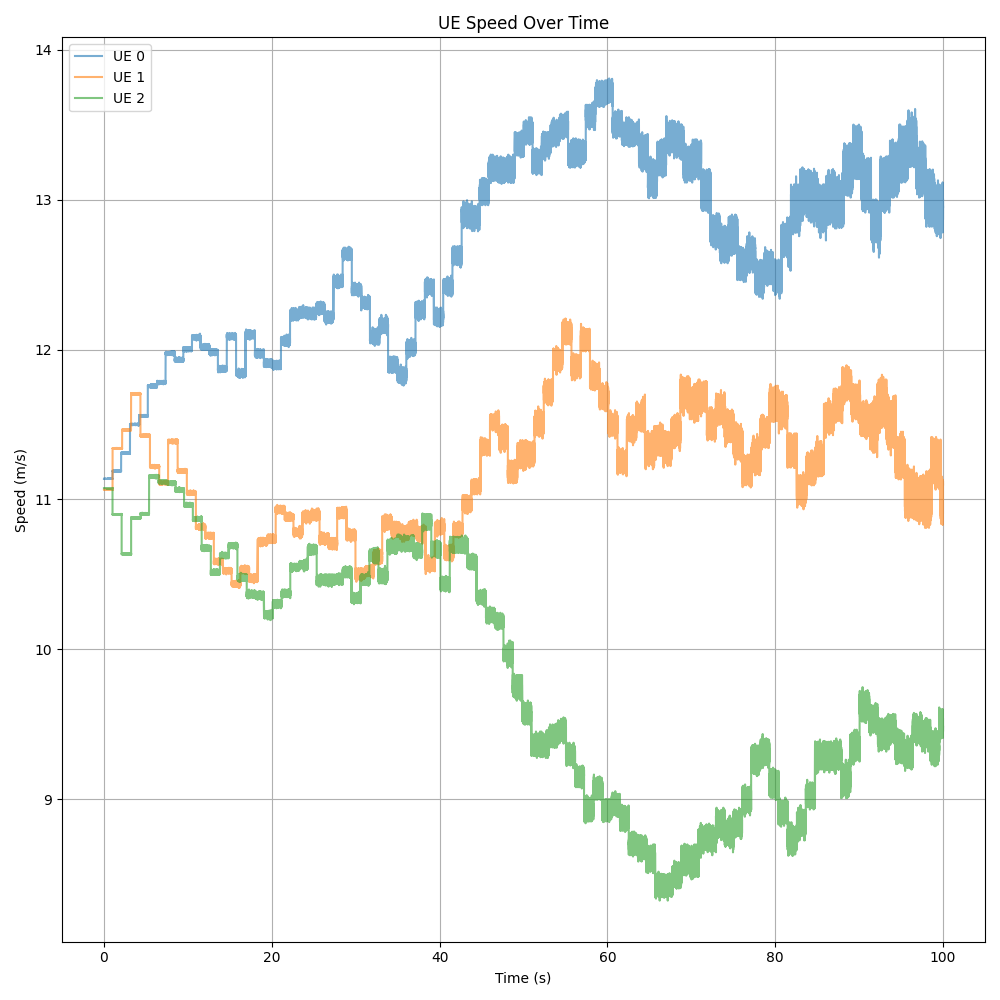
\includegraphics[scale=0.50]{../computos_y_graficas/v2x_5gmobix_num_0/5_9_11_32_6/ue/speed.png}}\end{center}

\begin{center}{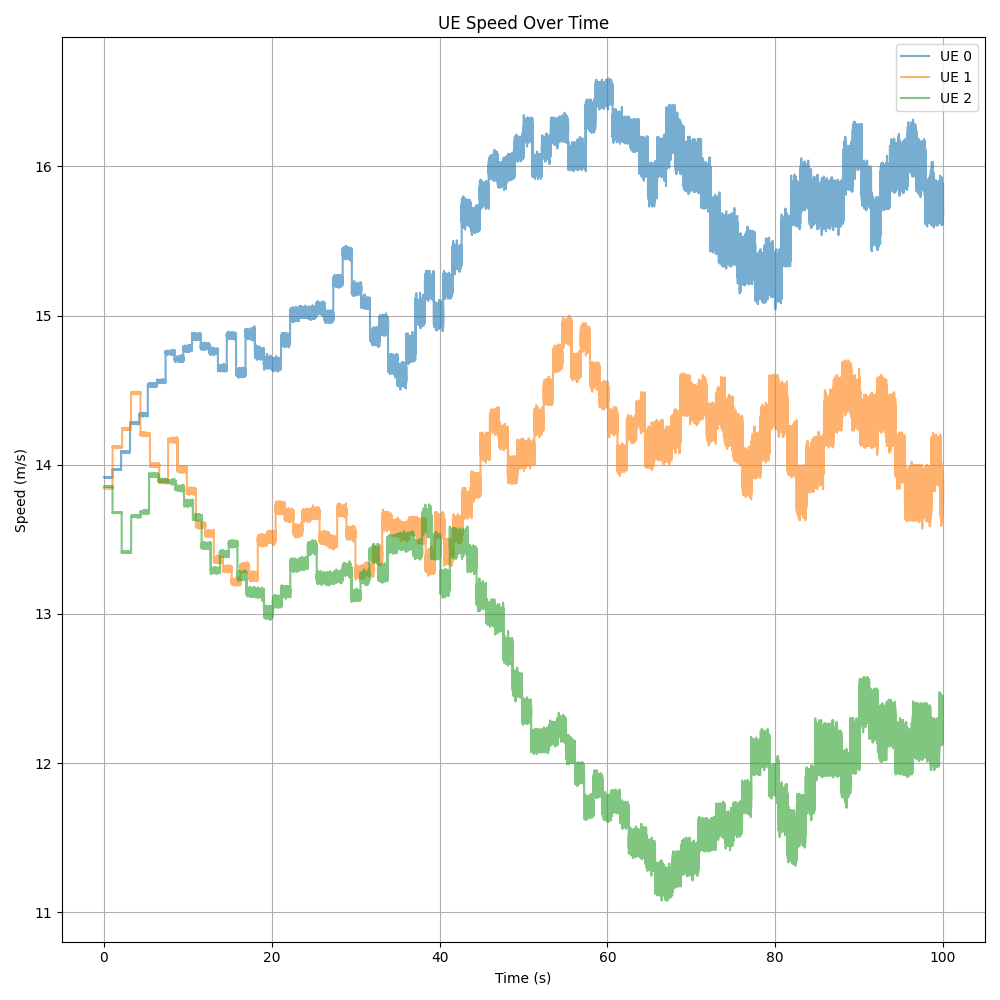
\includegraphics[scale=0.50]{../computos_y_graficas/v2x_5gmobix_num_0/5_9_11_33_46/ue/speed.png}}\end{center}

\begin{center}{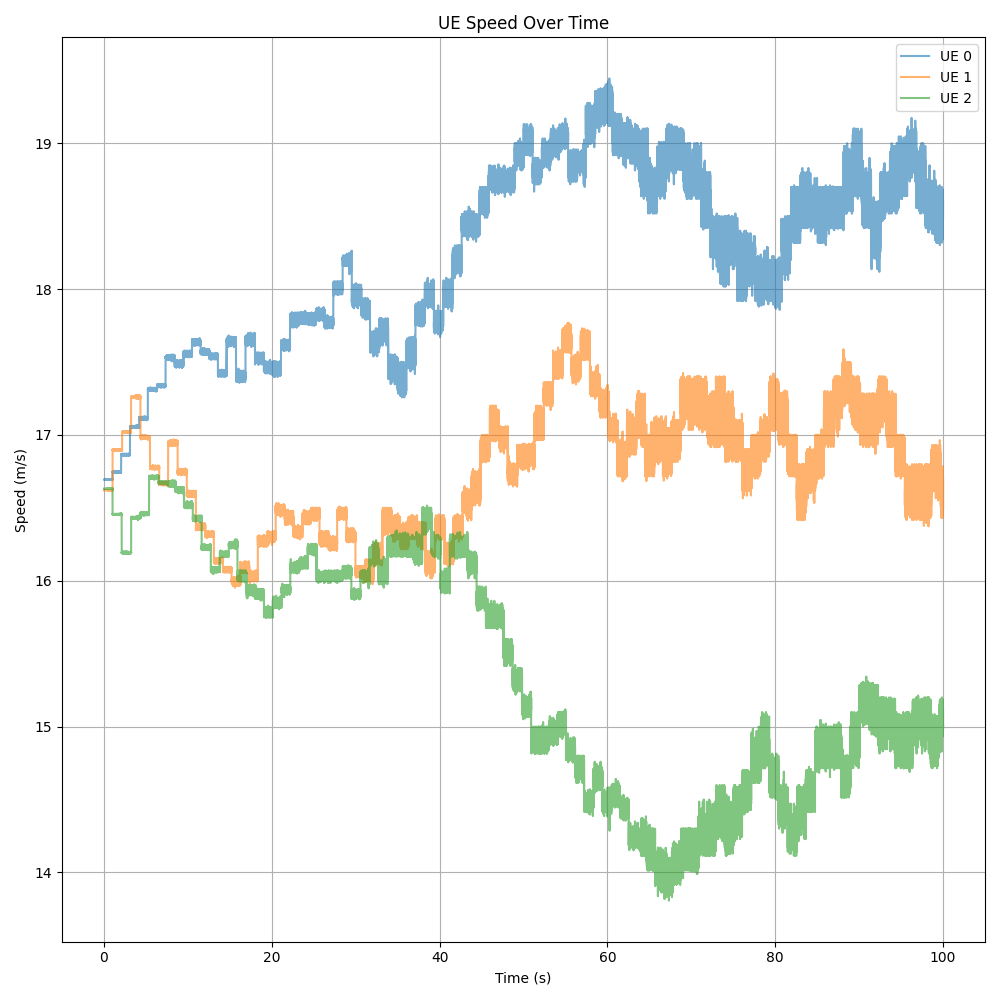
\includegraphics[scale=0.50]{../computos_y_graficas/v2x_5gmobix_num_0/5_9_11_35_26/ue/speed.png}}\end{center}

\begin{center}{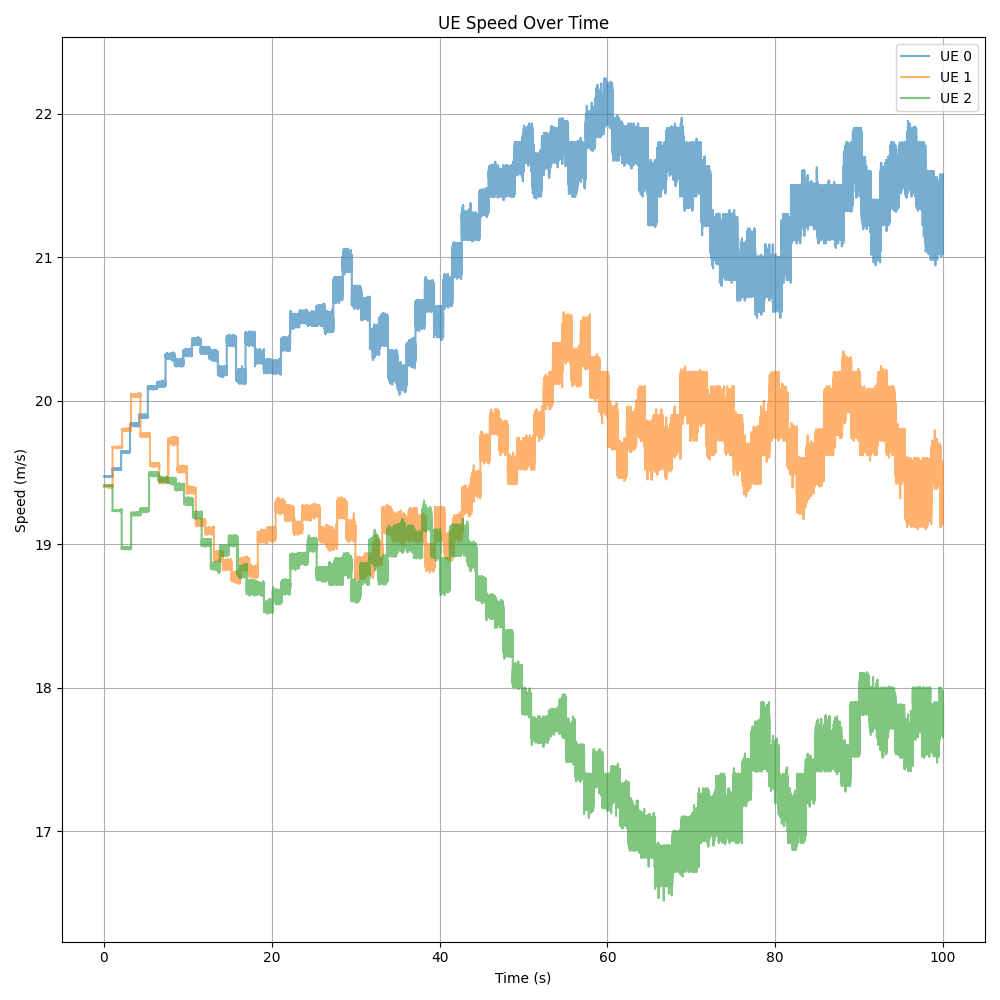
\includegraphics[scale=0.50]{../computos_y_graficas/v2x_5gmobix_num_0/5_9_11_37_6/ue/speed.png}}\end{center}

\begin{center}{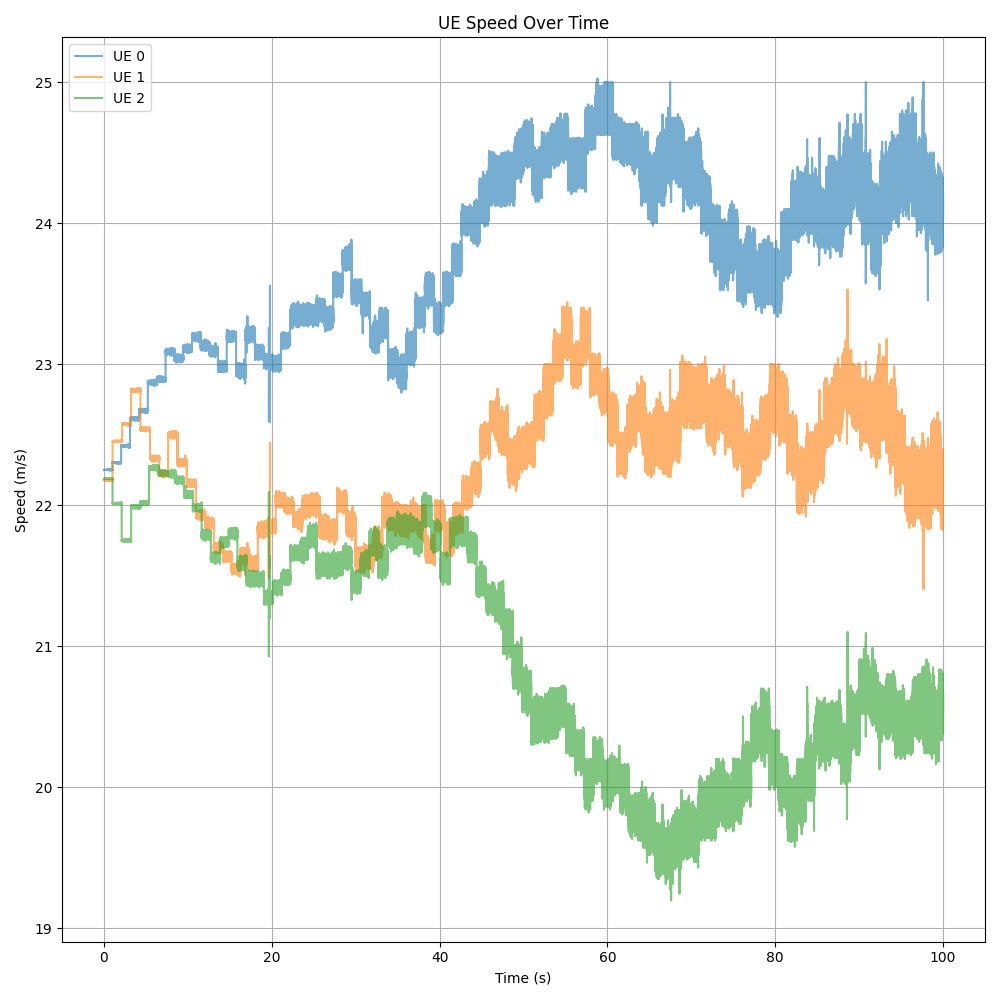
\includegraphics[scale=0.50]{../computos_y_graficas/v2x_5gmobix_num_0/5_9_11_38_47/ue/speed.png}}\end{center}

\begin{center}{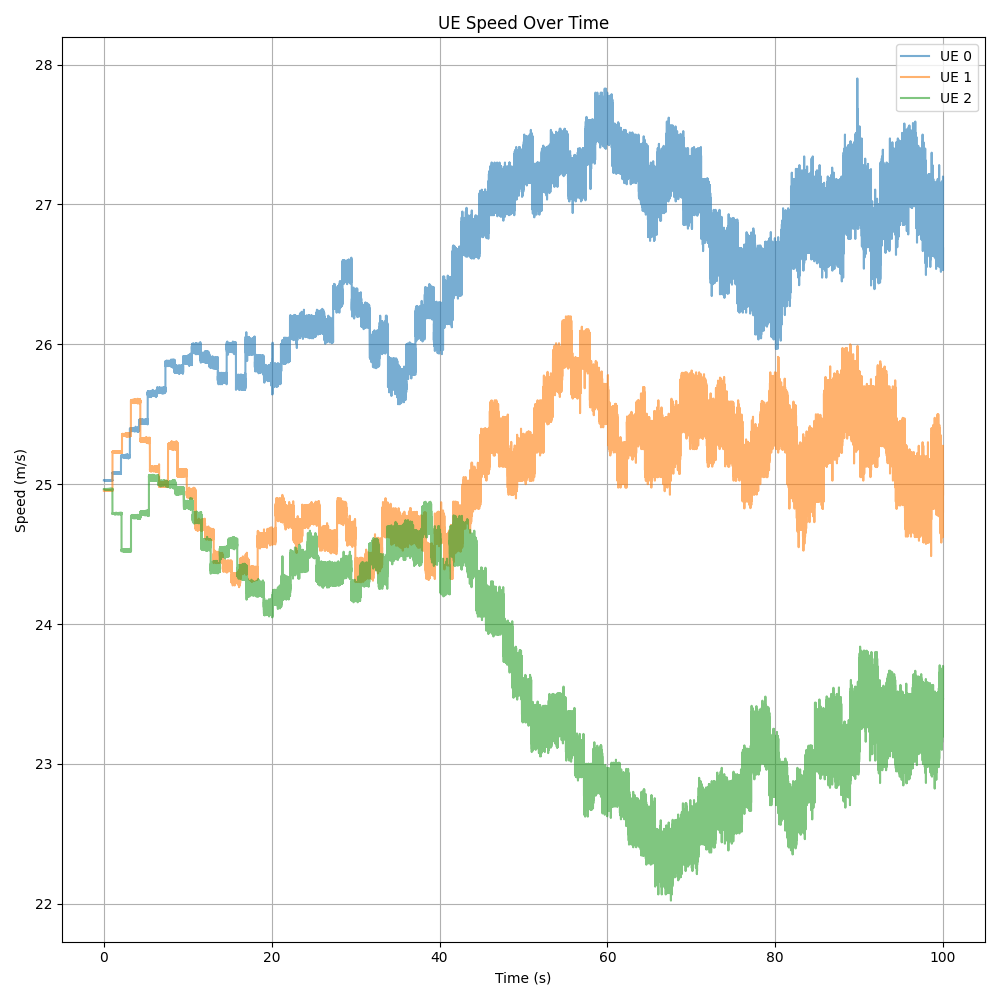
\includegraphics[scale=0.50]{../computos_y_graficas/v2x_5gmobix_num_0/5_9_11_40_27/ue/speed.png}}\end{center}

\begin{center}{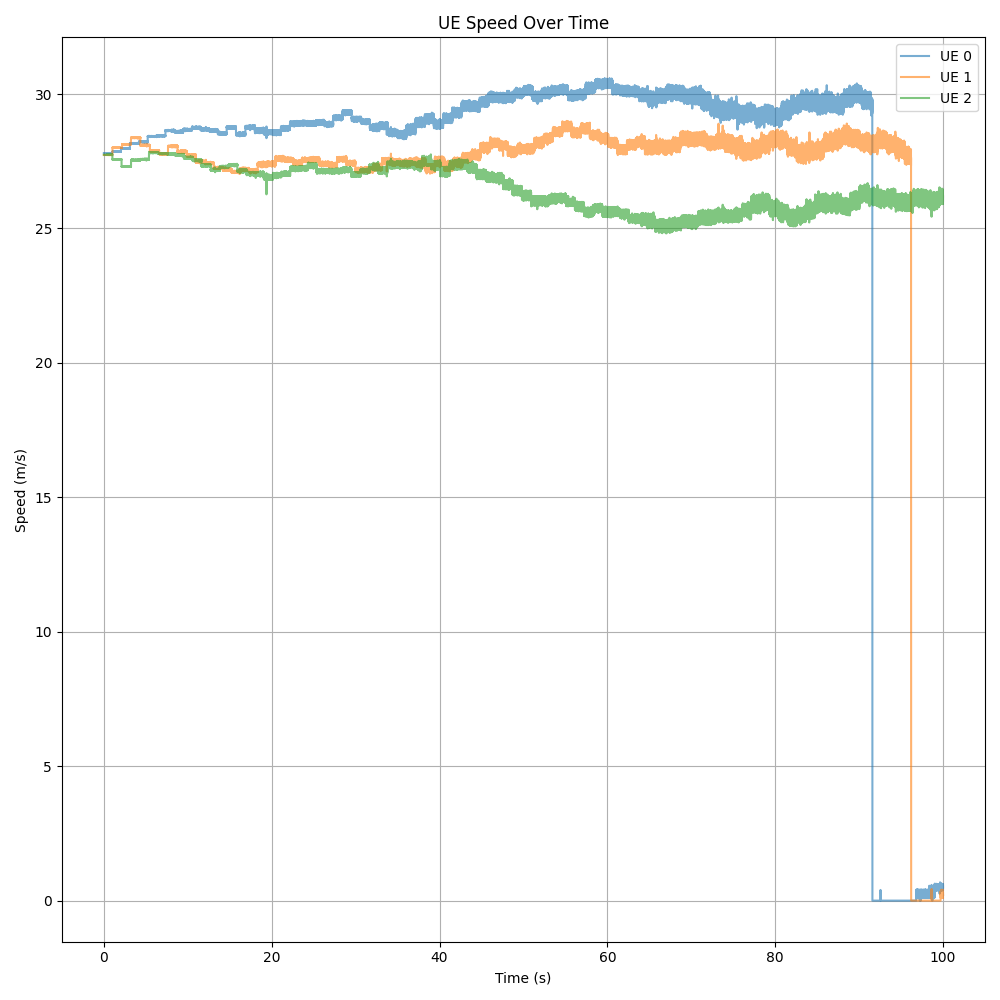
\includegraphics[scale=0.50]{../computos_y_graficas/v2x_5gmobix_num_0/5_9_11_42_7/ue/speed.png}}\end{center}

\begin{center}{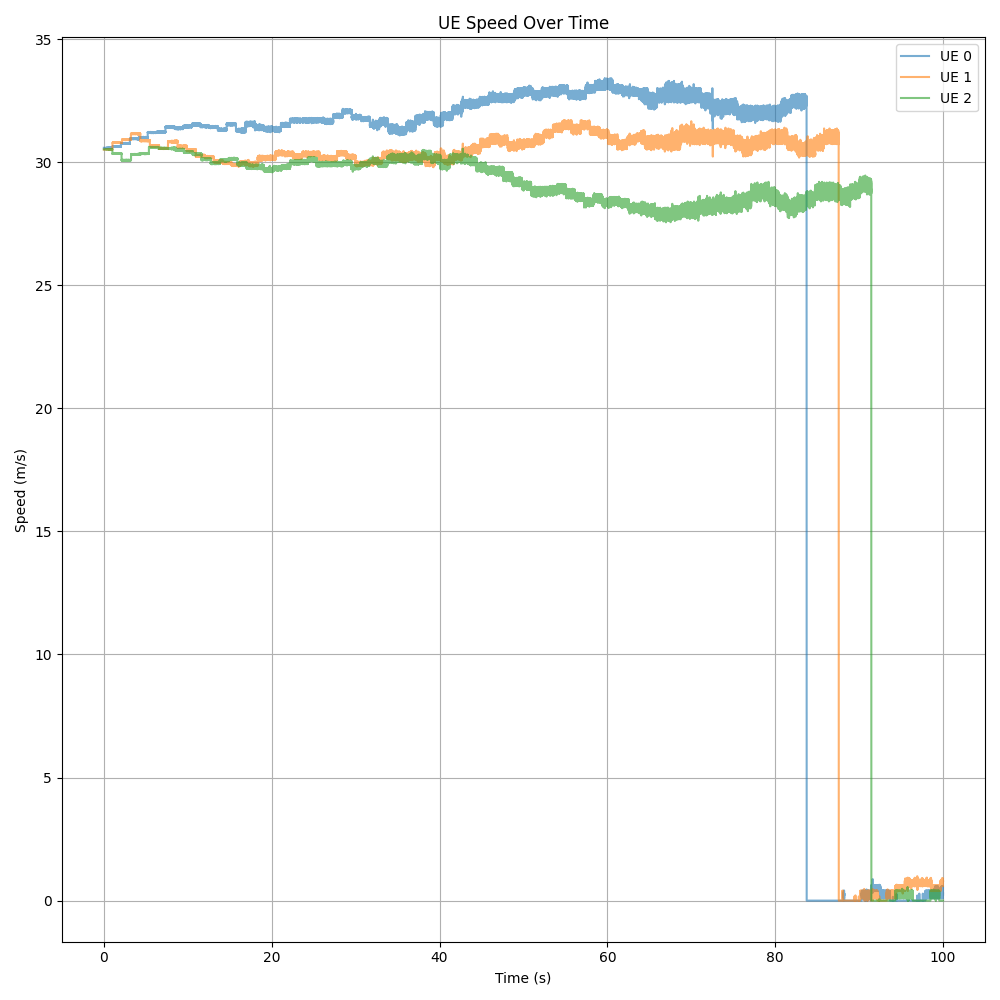
\includegraphics[scale=0.50]{../computos_y_graficas/v2x_5gmobix_num_0/5_9_11_43_47/ue/speed.png}}\end{center}

\begin{figure}[H]
	\ffigbox[\FBwidth] {
	\caption[C-V2X - Primer caso - Valocidad (I)]{Velocidad de los UE en tiempo real en las simulaciones del caso con numerología 0.

	(Fila 1): 10 km/h.

	(Fila 2): 20 km/h.

	(Fila 3): 30 km/h.

	(Fila 4): 40 km/h.

	(Fila 5): 50 km/h.

	(Fila 6): 60 km/h.

	(Fila 7): 70 km/h.

	(Fila 8): 80 km/h.

	(Fila 9): 90 km/h.

	(Fila 10): 100 km/h.

	(Fila 11): 110 km/h.

	(Fila 12): 120 km/h.}
	}
	{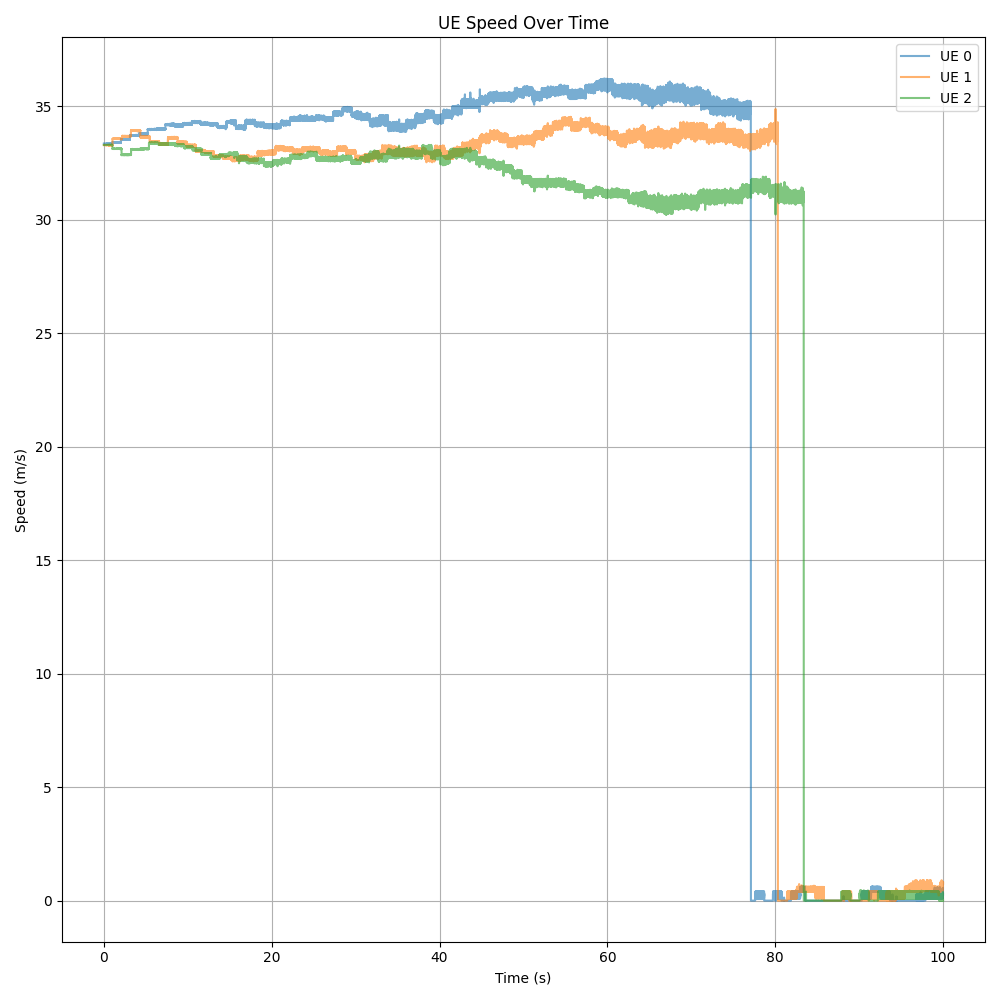
\includegraphics[scale=0.50]{../computos_y_graficas/v2x_5gmobix_num_0/5_9_11_45_27/ue/speed.png}}
\end{figure}

\subsubsection{Calidad del canal en el experimento 1}

%En primer lugar, podemos prever que las prestaciones de la red están limitadas por el ancho de banda, el ruido y la interferencia.
%Según la fórmula de Shannon (suponiendo una SINR de 200):
%$$
%C = W \log_2 \left( 1 + \frac {S} {N} \right) [b/s] = 10 [MHz] \cdot \log_2 \left( 1 + 200 \right) = 76,511 [Mbps]
%$$

\begin{center}{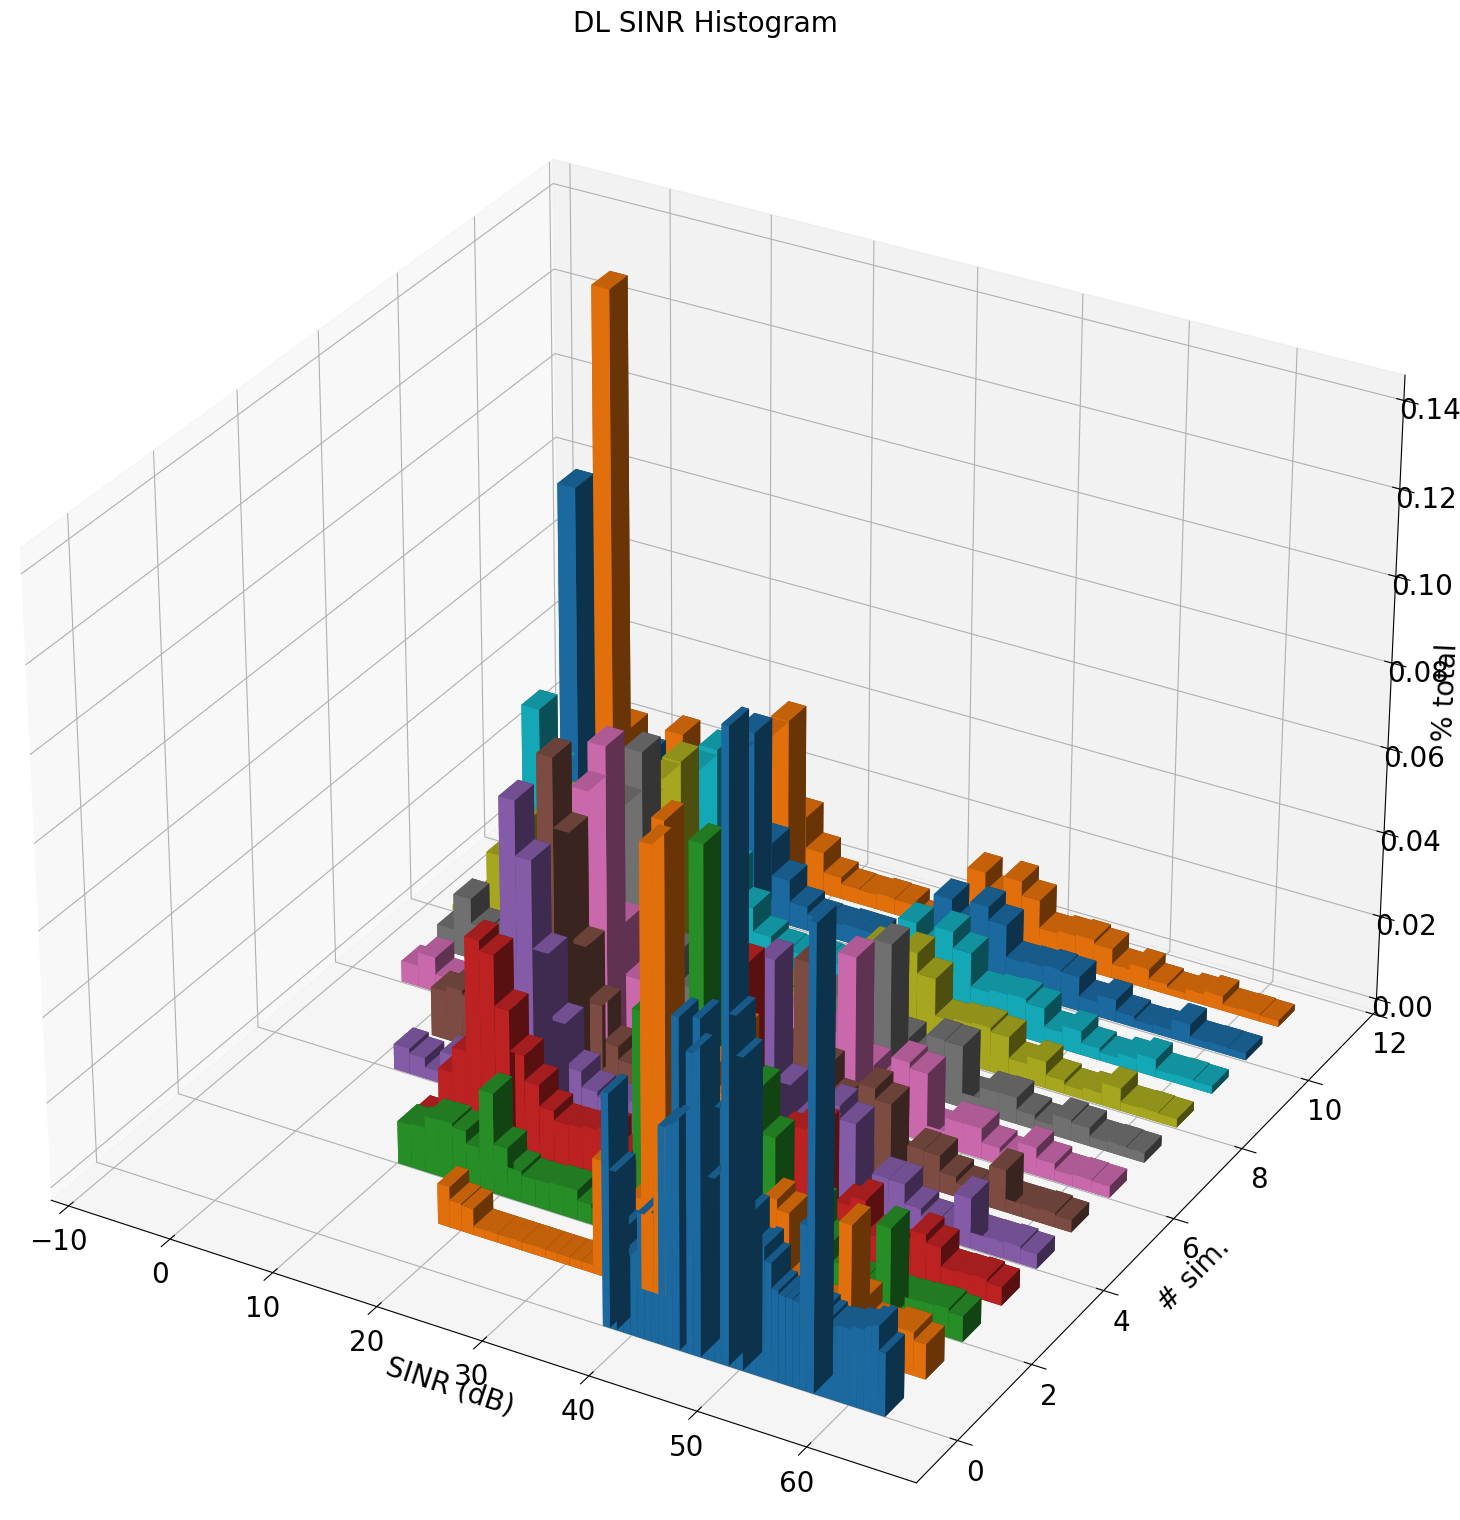
\includegraphics[scale=0.4]{../comparaciones/v2x_5gmobix_num_0/ue/sinr_dl_3d_hist_all_ue_multi.png_cropped.png}}\end{center}

\begin{center}{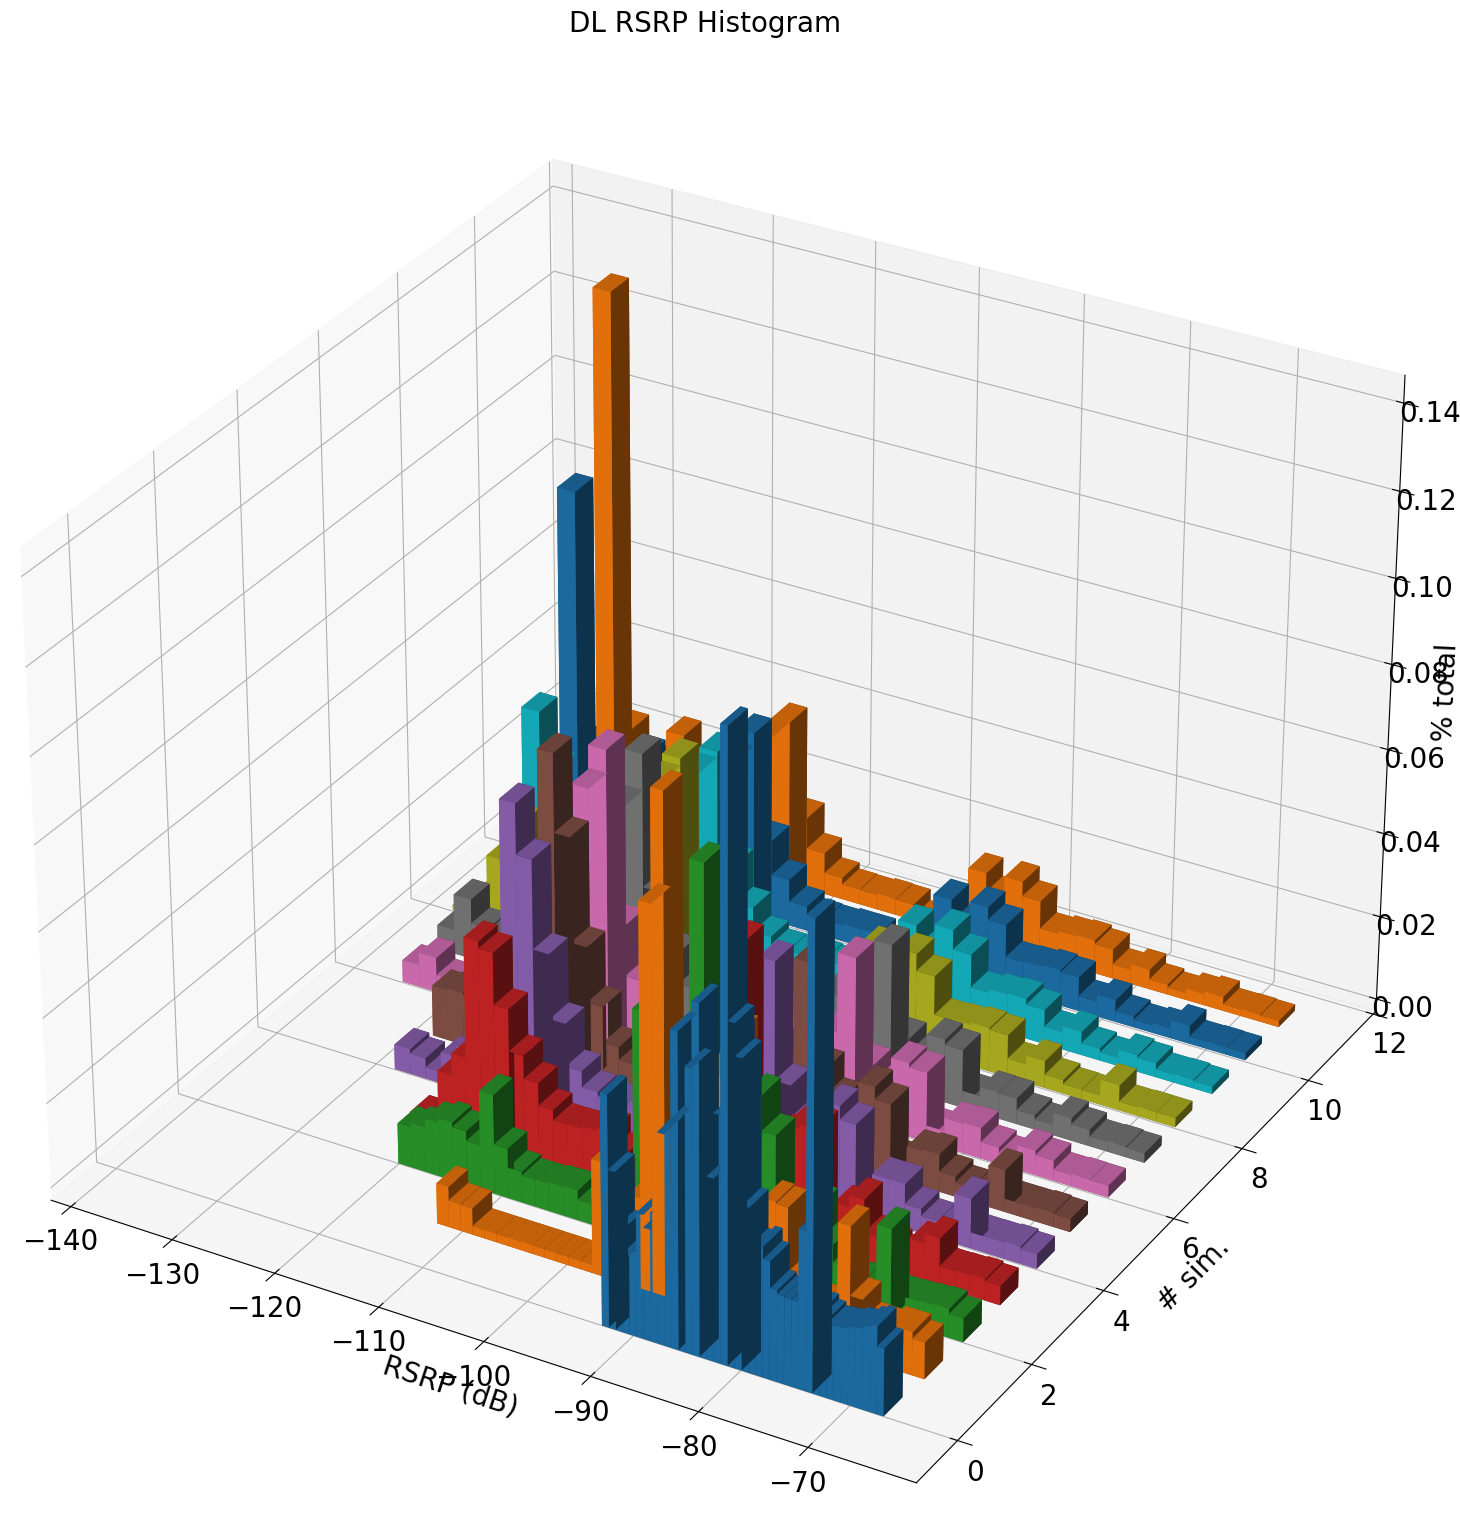
\includegraphics[scale=0.4]{../comparaciones/v2x_5gmobix_num_0/ue/rsrp_dl_3d_hist_all_ue_multi.png_cropped.png}}\end{center}

\begin{figure}[H]
	\ffigbox[\FBwidth] {
	\caption[C-V2X - Primer caso - Canal (I)]{Distribuciones de los indicadores del estado de canal para la dirección DL con la numerología 0.
	Las velocidades por orden: 10 km/h, 20 km/h, 30 km/h, 40 km/h, 50 km/h, 60 km/h, 70 km/h, 80 km/h, 90 km/h, 100 km/h, 120 km/h, 120 km/h.

	(Fila 1): SINR.

	(Fila 2): RSRP.

	(Fila 3): CQI.}
	}
	{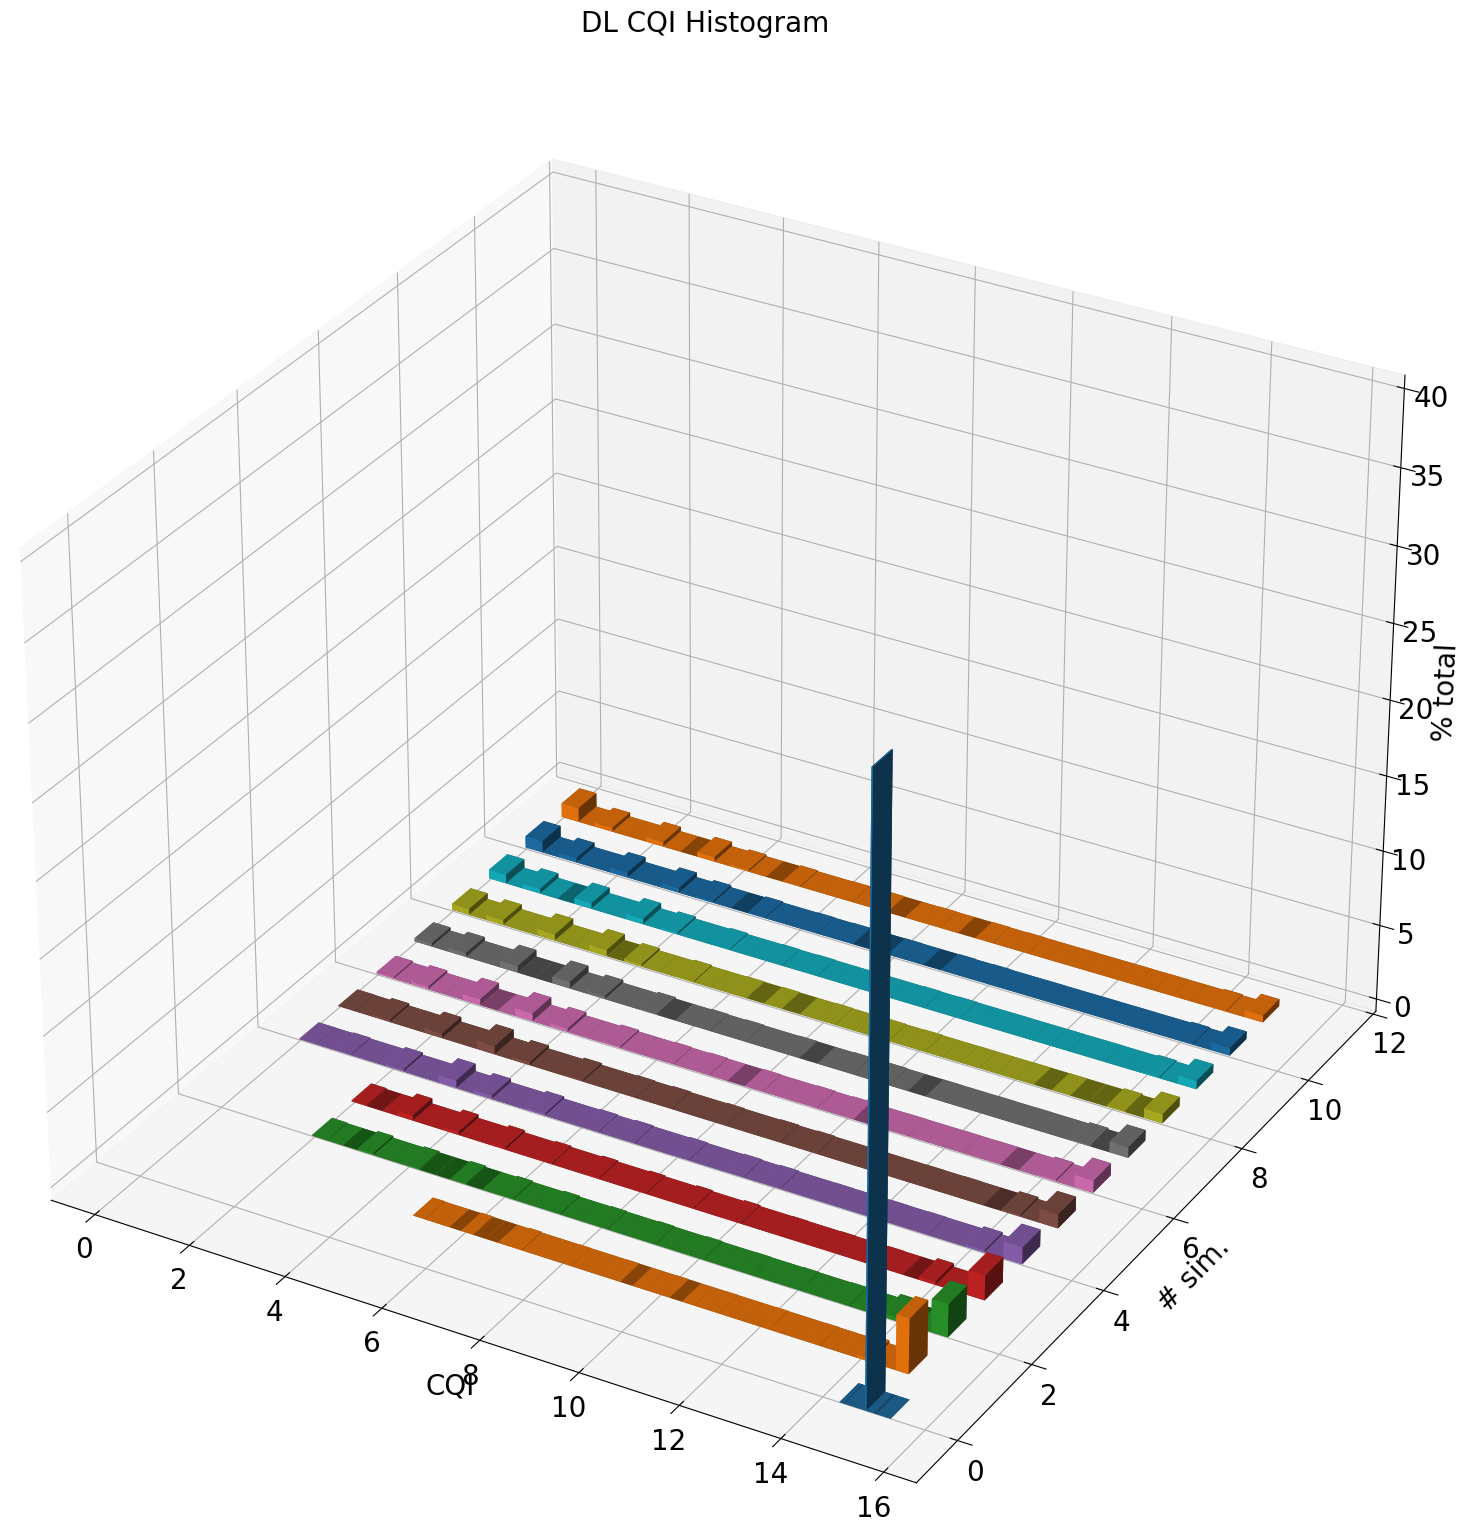
\includegraphics[scale=0.42]{../comparaciones/v2x_5gmobix_num_0/ue/cqi_dl_3d_hist_all_ue_multi.png_cropped.png}}
\end{figure}

\begin{center}{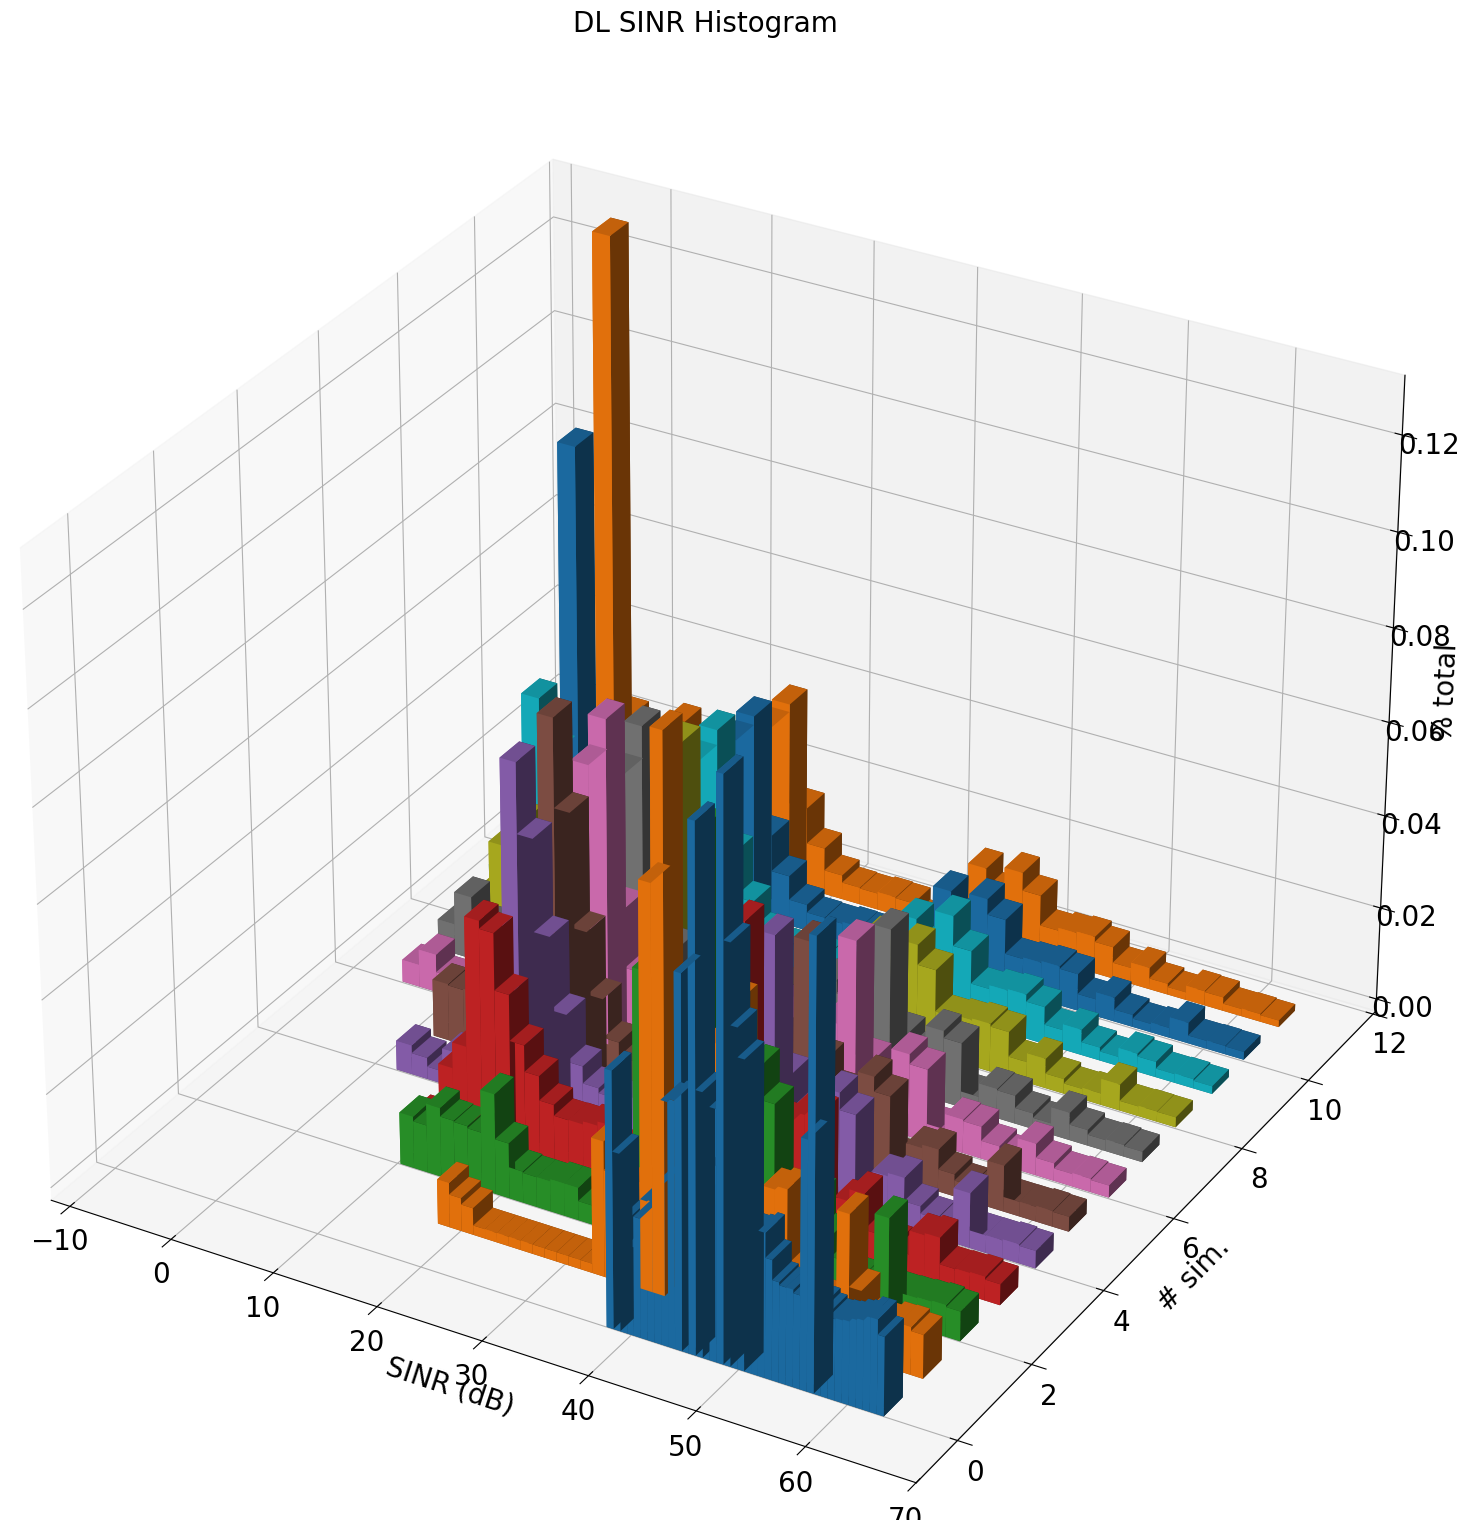
\includegraphics[scale=0.42]{../comparaciones/v2x_5gmobix_num_1/ue/sinr_dl_3d_hist_all_ue_multi.png_cropped.png}}\end{center}

\begin{center}{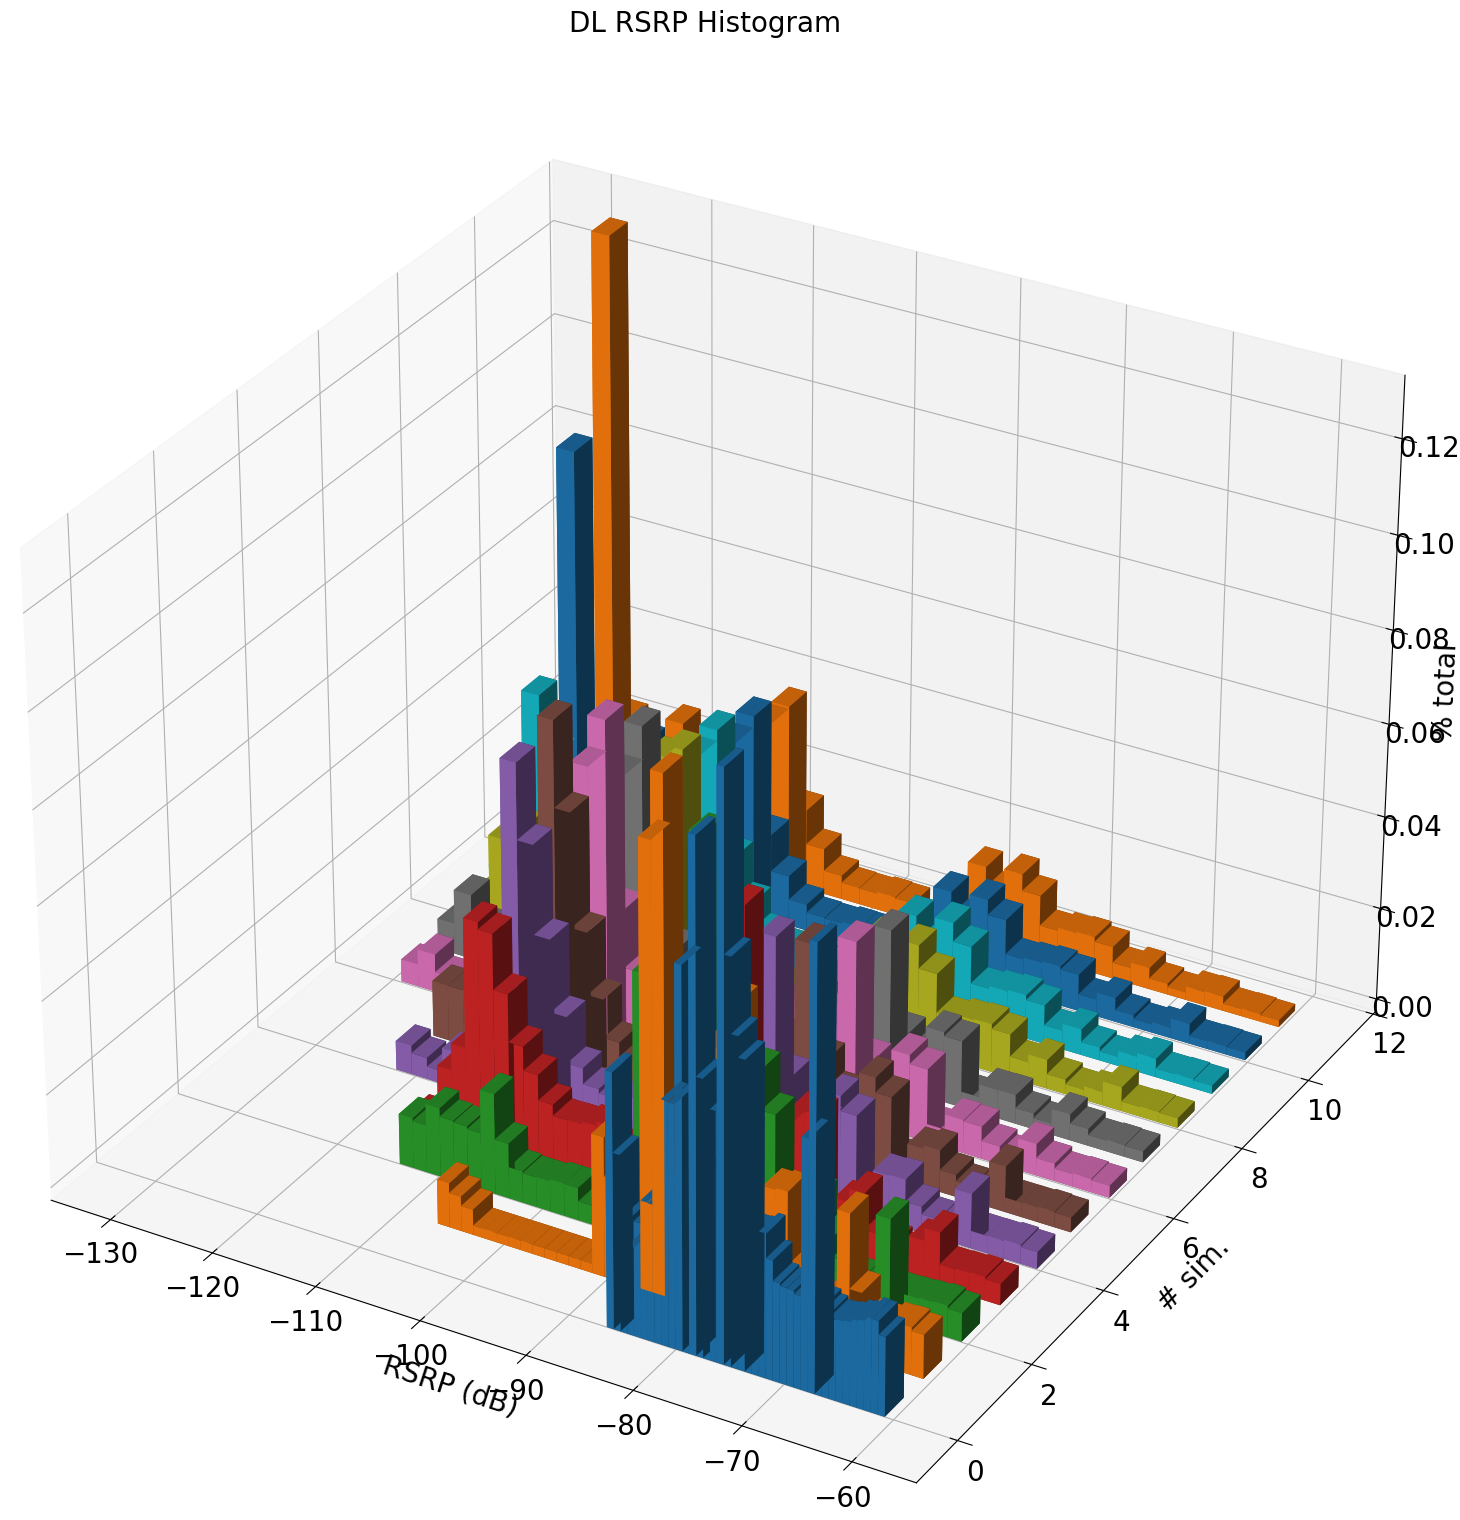
\includegraphics[scale=0.42]{../comparaciones/v2x_5gmobix_num_1/ue/rsrp_dl_3d_hist_all_ue_multi.png_cropped.png}}\end{center}

\begin{figure}[H]
	\ffigbox[\FBwidth] {
	\caption[C-V2X - Primer caso - Canal (II)]{Distribuciones de los indicadores del estado de canal para la dirección DL con la numerología 1.
	Las velocidades por orden: 10 km/h, 20 km/h, 30 km/h, 40 km/h, 50 km/h, 60 km/h, 70 km/h, 80 km/h, 90 km/h, 100 km/h, 120 km/h, 120 km/h.

	(Fila 1): SINR.

	(Fila 2): RSRP.

	(Fila 3): CQI.}
	}
	{\includegraphics[scale=0.42]{../comparaciones/v2x_5gmobix_num_1/ue/cqi_dl_3d_hist_all_ue_multi.png_cropped.png}}
\end{figure}

\begin{center}{\includegraphics[scale=0.42]{../comparaciones/v2x_5gmobix_num_2/ue/sinr_dl_3d_hist_all_ue_multi.png_cropped.png}}\end{center}

\begin{center}{\includegraphics[scale=0.42]{../comparaciones/v2x_5gmobix_num_2/ue/rsrp_dl_3d_hist_all_ue_multi.png_cropped.png}}\end{center}

\begin{figure}[H]
	\ffigbox[\FBwidth] {
	\caption[C-V2X - Primer caso - Canal (III)]{Distribuciones de los indicadores del estado de canal para la dirección DL con la numerología 2.
	Las velocidades por orden: 10 km/h, 20 km/h, 30 km/h, 40 km/h, 50 km/h, 60 km/h, 70 km/h, 80 km/h, 90 km/h, 100 km/h, 120 km/h, 120 km/h.

	(Fila 1): SINR.

	(Fila 2): RSRP.

	(Fila 3): CQI.}
	}
	{\includegraphics[scale=0.42]{../comparaciones/v2x_5gmobix_num_2/ue/cqi_dl_3d_hist_all_ue_multi.png_cropped.png}}
\end{figure}

\begin{center}{\includegraphics[scale=0.42]{../comparaciones/v2x_5gmobix_num_3/ue/sinr_dl_3d_hist_all_ue_multi.png_cropped.png}}\end{center}

\begin{center}{\includegraphics[scale=0.42]{../comparaciones/v2x_5gmobix_num_3/ue/rsrp_dl_3d_hist_all_ue_multi.png_cropped.png}}\end{center}

\begin{figure}[H]
	\ffigbox[\FBwidth] {
	\caption[C-V2X - Primer caso - Canal (IV)]{Distribuciones de los indicadores del estado de canal para la dirección DL con la numerología 3.
	Las velocidades por orden: 10 km/h, 20 km/h, 30 km/h, 40 km/h, 50 km/h, 60 km/h, 70 km/h, 80 km/h, 90 km/h, 100 km/h, 120 km/h, 120 km/h.

	(Fila 1): SINR.

	(Fila 2): RSRP.

	(Fila 3): CQI.}
	}
	{\includegraphics[scale=0.42]{../comparaciones/v2x_5gmobix_num_3/ue/cqi_dl_3d_hist_all_ue_multi.png_cropped.png}}
\end{figure}

\begin{center}{\includegraphics[scale=0.42]{../comparaciones/v2x_5gmobix_num_4/ue/sinr_dl_3d_hist_all_ue_multi.png_cropped.png}}\end{center}

\begin{center}{\includegraphics[scale=0.42]{../comparaciones/v2x_5gmobix_num_4/ue/rsrp_dl_3d_hist_all_ue_multi.png_cropped.png}}\end{center}

\begin{figure}[H]
	\ffigbox[\FBwidth] {
	\caption[C-V2X - Primer caso - Canal (V)]{Distribuciones de los indicadores del estado de canal para la dirección DL con la numerología 4.
	Las velocidades por orden: 10 km/h, 20 km/h, 30 km/h, 40 km/h, 50 km/h, 60 km/h, 70 km/h, 80 km/h, 90 km/h, 100 km/h, 120 km/h, 120 km/h.

	(Fila 1): SINR.

	(Fila 2): RSRP.

	(Fila 3): CQI.}
	}
	{\includegraphics[scale=0.42]{../comparaciones/v2x_5gmobix_num_4/ue/cqi_dl_3d_hist_all_ue_multi.png_cropped.png}}
\end{figure}

\begin{center}{\includegraphics[scale=0.42]{../comparaciones/v2x_5gmobix_num_5/ue/sinr_dl_3d_hist_all_ue_multi.png_cropped.png}}\end{center}

\begin{center}{\includegraphics[scale=0.42]{../comparaciones/v2x_5gmobix_num_5/ue/rsrp_dl_3d_hist_all_ue_multi.png_cropped.png}}\end{center}

\begin{figure}[H]
	\ffigbox[\FBwidth] {
	\caption[C-V2X - Primer caso - Canal (VI)]{Distribuciones de los indicadores del estado de canal para la dirección DL con la numerología 5.
	Las velocidades por orden: 10 km/h, 20 km/h, 30 km/h, 40 km/h, 50 km/h, 60 km/h, 70 km/h, 80 km/h, 90 km/h, 100 km/h, 120 km/h, 120 km/h.

	(Fila 1): SINR.

	(Fila 2): RSRP.

	(Fila 3): CQI.}
	}
	{\includegraphics[scale=0.42]{../comparaciones/v2x_5gmobix_num_5/ue/cqi_dl_3d_hist_all_ue_multi.png_cropped.png}}
\end{figure}

Si atendemos a los valores indicativos del estado del canal de transmisión (SINR, RSRP, CQI), en las figuras 5.3, 5.4, 5.5, 5.6, 5.7 y 5.8,
podemos ver que éstos cambian entre velocidades y numerologías de manera significativa.
El empeoramiento del canal con mayores velocidades es de esperar, pues los UE se alejan de la gNB  y la propagación empeora.
Por otro lado, vemos, por ejemplo, que la SINR se concentra en valores de 40 dB, 45 dB, 50 dB, 50 dB, 50 dB, 50 dB en las numerologías 0 (figura 5.3), 1 (figura 5.4), 2 (figura 5.5), 3 (figura 5.6), 4 (figura 5.7), 5 (figura 5.8), respectivamente;
al aumentar el espaciado entre subportadoras con los mayores índices de numerología, aumenta la SINR y, de igual manera, los otros indicadores.

\begin{figure}[H]
	\ffigbox[\FBwidth] {
	\caption[C-V2X - Primer caso - MCS (I)]{Distribución del índice MCS para la dirección DL con la numerología 0.
	Las velocidades por orden: 10 km/h, 20 km/h, 30 km/h, 40 km/h, 50 km/h, 60 km/h, 70 km/h, 80 km/h, 90 km/h, 100 km/h, 120 km/h, 120 km/h.}
	}
	{\includegraphics[scale=0.42]{../comparaciones/v2x_5gmobix_num_0/ue/mcs_dl_3d_hist_all_ue_multi.png_cropped.png}}
\end{figure}

\begin{figure}[H]
	\ffigbox[\FBwidth] {
	\caption[C-V2X - Primer caso - MCS (II)]{Distribución del índice MCS para la dirección DL con la numerología 1.
	Las velocidades por orden: 10 km/h, 20 km/h, 30 km/h, 40 km/h, 50 km/h, 60 km/h, 70 km/h, 80 km/h, 90 km/h, 100 km/h, 120 km/h, 120 km/h.}
	}
	{\includegraphics[scale=0.42]{../comparaciones/v2x_5gmobix_num_1/ue/mcs_dl_3d_hist_all_ue_multi.png_cropped.png}}
\end{figure}

\begin{figure}[H]
	\ffigbox[\FBwidth] {
	\caption[C-V2X - Primer caso - MCS (III)]{Distribución del índice MCS para la dirección DL con la numerología 2.
	Las velocidades por orden: 10 km/h, 20 km/h, 30 km/h, 40 km/h, 50 km/h, 60 km/h, 70 km/h, 80 km/h, 90 km/h, 100 km/h, 120 km/h, 120 km/h.}
	}
	{\includegraphics[scale=0.42]{../comparaciones/v2x_5gmobix_num_2/ue/mcs_dl_3d_hist_all_ue_multi.png_cropped.png}}
\end{figure}

\begin{figure}[H]
	\ffigbox[\FBwidth] {
	\caption[C-V2X - Primer caso - MCS (IV)]{Distribución del índice MCS para la dirección DL con la numerología 3.
	Las velocidades por orden: 10 km/h, 20 km/h, 30 km/h, 40 km/h, 50 km/h, 60 km/h, 70 km/h, 80 km/h, 90 km/h, 100 km/h, 120 km/h, 120 km/h.}
	}
	{\includegraphics[scale=0.42]{../comparaciones/v2x_5gmobix_num_3/ue/mcs_dl_3d_hist_all_ue_multi.png_cropped.png}}
\end{figure}

\begin{figure}[H]
	\ffigbox[\FBwidth] {
	\caption[C-V2X - Primer caso - MCS (V)]{Distribución del índice MCS para la dirección DL con la numerología 4.
	Las velocidades por orden: 10 km/h, 20 km/h, 30 km/h, 40 km/h, 50 km/h, 60 km/h, 70 km/h, 80 km/h, 90 km/h, 100 km/h, 120 km/h, 120 km/h.}
	}
	{\includegraphics[scale=0.42]{../comparaciones/v2x_5gmobix_num_4/ue/mcs_dl_3d_hist_all_ue_multi.png_cropped.png}}
\end{figure}

\begin{figure}[H]
	\ffigbox[\FBwidth] {
	\caption[C-V2X - Primer caso - MCS (VI)]{Distribución del índice MCS para la dirección DL con la numerología 5.
	Las velocidades por orden: 10 km/h, 20 km/h, 30 km/h, 40 km/h, 50 km/h, 60 km/h, 70 km/h, 80 km/h, 90 km/h, 100 km/h, 120 km/h, 120 km/h.}
	}
	{\includegraphics[scale=0.42]{../comparaciones/v2x_5gmobix_num_5/ue/mcs_dl_3d_hist_all_ue_multi.png_cropped.png}}
\end{figure}

En las figuras 5.9, 5.10, 5.11, 5.12, 5.13 y 5.14 podemos ver que,
de manera paralela, el índice MCS cambia entre velocidades y numerologías.
Además, se concentra en los valores de 0 y 27:
Este resultado es, igualmente, esperable, pues los valores SINR, CQI, etc. son los que determinan el valor MCS elegido.
En especial, la numerología 5 (figura 5.14) es la que más modifica el MCS para permitir la transmisión.

\subsubsection{Prestaciones en el experimento}

\begin{center}{\includegraphics[scale=0.42]{../comparaciones/v2x_5gmobix_num_0/ue/ildl_3d_hist_all_ue_multi.png_cropped.png}}\end{center}

\begin{center}{\includegraphics[scale=0.42]{../comparaciones/v2x_5gmobix_num_0/ue/ilul_3d_hist_all_ue_multi.png_cropped.png}}\end{center}

\begin{center}{\includegraphics[scale=0.42]{../comparaciones/v2x_5gmobix_num_1/ue/ildl_3d_hist_all_ue_multi.png_cropped.png}}\end{center}

\begin{center}{\includegraphics[scale=0.42]{../comparaciones/v2x_5gmobix_num_1/ue/ilul_3d_hist_all_ue_multi.png_cropped.png}}\end{center}

\begin{center}{\includegraphics[scale=0.42]{../comparaciones/v2x_5gmobix_num_2/ue/ildl_3d_hist_all_ue_multi.png_cropped.png}}\end{center}

\begin{center}{\includegraphics[scale=0.42]{../comparaciones/v2x_5gmobix_num_2/ue/ilul_3d_hist_all_ue_multi.png_cropped.png}}\end{center}

\begin{center}{\includegraphics[scale=0.42]{../comparaciones/v2x_5gmobix_num_3/ue/ildl_3d_hist_all_ue_multi.png_cropped.png}}\end{center}

\begin{center}{\includegraphics[scale=0.42]{../comparaciones/v2x_5gmobix_num_3/ue/ilul_3d_hist_all_ue_multi.png_cropped.png}}\end{center}

\begin{center}{\includegraphics[scale=0.42]{../comparaciones/v2x_5gmobix_num_4/ue/ildl_3d_hist_all_ue_multi.png_cropped.png}}\end{center}

\begin{center}{\includegraphics[scale=0.42]{../comparaciones/v2x_5gmobix_num_4/ue/ilul_3d_hist_all_ue_multi.png_cropped.png}}\end{center}

\begin{center}{\includegraphics[scale=0.42]{../comparaciones/v2x_5gmobix_num_5/ue/ildl_3d_hist_all_ue_multi.png_cropped.png}}\end{center}

\begin{center}{\includegraphics[scale=0.42]{../comparaciones/v2x_5gmobix_num_5/ue/ilul_3d_hist_all_ue_multi.png_cropped.png}}\end{center}

\begin{figure}[H]
	\ffigbox[\FBwidth] {
	\caption[C-V2X - Primer caso - Latencia (I)]{Distribución de la latencia de paquetes IP..

	(Fila 1): Resultados de obtenidos con la numerología 0 en dirección DL.

	(Fila 2): Resultados de obtenidos con la numerología 0 en dirección UL.

	(Fila 3): Resultados de obtenidos con la numerología 1 en dirección DL.

	(Fila 4): Resultados de obtenidos con la numerología 1 en dirección UL.

	(Fila 5): Resultados de obtenidos con la numerología 2 en dirección DL.

	(Fila 6): Resultados de obtenidos con la numerología 2 en dirección UL.

	(Fila 7): Resultados de obtenidos con la numerología 3 en dirección DL.

	(Fila 8): Resultados de obtenidos con la numerología 3 en dirección UL.

	(Fila 9): Resultados de obtenidos con la numerología 4 en dirección DL.

	(Fila 10): Resultados de obtenidos con la numerología 4 en dirección UL.

	(Fila 11): Resultados de obtenidos con la numerología 5 en dirección DL.

	(Fila 12): Resultados de obtenidos con la numerología 5 en dirección UL.

	(Fila 13): Resultados de \cite{RefWorks:25}.}
	}
	{\includegraphics[scale=0.3]{imagenes/v2x_5gmobix/v2x_5gmobix-007.png}}
\end{figure}

Se trata de una aplicación que requiere buenas prestaciones de latencia y fiabilidad.
En primer lugar, comparamos la latencia de \cite{RefWorks:25} con la simulada, mostrado en la figura 5.15.
En todas las simulaciones se puede ver que, con velocidades bajas (10 km/h - 40 km/h), las latencias se concentran en valores muy bajos;
en torno a 50 km/h - 60 km/h empiezan a apreciarse latencias importantes y, a partir de 70 km/h, se dispara.
Como anteriormente se indicó, esto se debe al hecho de que en las simulaciones de mayor velocidad, el UE se encuentra más alejado de la gNB;
el canal es peor, se recurre a más retransmisiones de HARQ y los paquetes tardan más en entregarse.
Por lo tanto, la velocidad no es, de manera directa, un factor que genere latencia;
ya se explicó que el emulador \textit{FikoRE}, y el sistema 5G en general, atienden al fenómeno del multitrayecto y la dispersión Doppler, por lo que no le podemos atribuir la latencia a este fenómeno.
En cualquier caso, en el experimento con un despliegue real en \cite{RefWorks:25} las latencias apenas superan los 25 ms, con las medias (triángulo morado) por debajo de 20 ms y las medianas (línea roja) próximas a 10 ms;
tanto la simulación como la experiencia demuestra que los terminales en movimiento, por lo general, no experimentan grandes latencias.
Hay que matizar que en el experimento en \cite{RefWorks:25} también tiene lugar un traspaso.

\begin{center}{\includegraphics[scale=0.6]{../computos_y_graficas/v2x_5gmobix_num_0/5_9_11_19_47/ue/distance.png}}\end{center}

\begin{center}{\includegraphics[scale=0.6]{../computos_y_graficas/v2x_5gmobix_num_0/5_9_11_19_47/ue/acceleration.png}}\end{center}

\begin{center}{\includegraphics[scale=0.4]{../computos_y_graficas/v2x_5gmobix_num_0/5_9_11_19_47/mac/dl_throughput.png}}\end{center}

\begin{center}{\includegraphics[scale=0.4]{../computos_y_graficas/v2x_5gmobix_num_0/5_9_11_19_47/mac/ul_throughput.png}}\end{center}

\begin{center}{\includegraphics[scale=0.6]{../computos_y_graficas/v2x_5gmobix_num_0/5_9_11_19_47/ue/ildl_instantaneous.png}}\end{center}

\begin{figure}[H]
	\ffigbox[\FBwidth] {
	\caption[C-V2X - Primer caso - Mezcla de resultados (I)]{Resultados a 10 km/h con la numerología 0.

	(Fila 1): Distancia a la gNB en tiempo real.

	(Fila 2): Aceleración en tiempo real.

	(Fila 3): Tasa binaria en tiempo real en dirección DL.

	(Fila 4): Tasa binaria en tiempo real en dirección UL.

	(Fila 5): Latencia de los paquetes IP en tiempo real en dirección DL.

	(Fila 6): Latencia de los paquetes IP en tiempo real en dirección UL.}
	}
	{\includegraphics[scale=0.6]{../computos_y_graficas/v2x_5gmobix_num_0/5_9_11_19_47/ue/ilul_instantaneous.png}}
\end{figure}

\begin{center}{\includegraphics[scale=0.6]{../computos_y_graficas/v2x_5gmobix_num_0/5_9_11_30_26/ue/distance.png}}\end{center}

\begin{center}{\includegraphics[scale=0.6]{../computos_y_graficas/v2x_5gmobix_num_0/5_9_11_30_26/ue/acceleration.png}}\end{center}

\begin{center}{\includegraphics[scale=0.4]{../computos_y_graficas/v2x_5gmobix_num_0/5_9_11_30_26/mac/dl_throughput.png}}\end{center}

\begin{center}{\includegraphics[scale=0.4]{../computos_y_graficas/v2x_5gmobix_num_0/5_9_11_30_26/mac/ul_throughput.png}}\end{center}

\begin{center}{\includegraphics[scale=0.6]{../computos_y_graficas/v2x_5gmobix_num_0/5_9_11_30_26/ue/ildl_instantaneous.png}}\end{center}

\begin{figure}[H]
	\ffigbox[\FBwidth] {
	\caption[C-V2X - Primer caso - Mezcla de resultados (II)]{Resultados a 30 km/h con la numerología 0.

	(Fila 1): Distancia a la gNB en tiempo real.

	(Fila 2): Aceleración en tiempo real.

	(Fila 3): Tasa binaria en tiempo real en dirección DL.

	(Fila 4): Tasa binaria en tiempo real en dirección UL.

	(Fila 5): Latencia de los paquetes IP en tiempo real en dirección DL.

	(Fila 6): Latencia de los paquetes IP en tiempo real en dirección UL.}
	}
	{\includegraphics[scale=0.6]{../computos_y_graficas/v2x_5gmobix_num_0/5_9_11_30_26/ue/ilul_instantaneous.png}}
\end{figure}

\begin{center}{\includegraphics[scale=0.6]{../computos_y_graficas/v2x_5gmobix_num_0/5_9_11_35_26/ue/distance.png}}\end{center}

\begin{center}{\includegraphics[scale=0.6]{../computos_y_graficas/v2x_5gmobix_num_0/5_9_11_35_26/ue/acceleration.png}}\end{center}

\begin{center}{\includegraphics[scale=0.4]{../computos_y_graficas/v2x_5gmobix_num_0/5_9_11_35_26/mac/dl_throughput.png}}\end{center}

\begin{center}{\includegraphics[scale=0.4]{../computos_y_graficas/v2x_5gmobix_num_0/5_9_11_35_26/mac/ul_throughput.png}}\end{center}

\begin{center}{\includegraphics[scale=0.6]{../computos_y_graficas/v2x_5gmobix_num_0/5_9_11_35_26/ue/ildl_instantaneous.png}}\end{center}

\begin{figure}[H]
	\ffigbox[\FBwidth] {
	\caption[C-V2X - Primer caso - Mezcla de resultados (III)]{Resultados a 60 km/h con la numerología 0.

	(Fila 1): Distancia a la gNB en tiempo real.

	(Fila 2): Aceleración en tiempo real.

	(Fila 3): Tasa binaria en tiempo real en dirección DL.

	(Fila 4): Tasa binaria en tiempo real en dirección UL.

	(Fila 5): Latencia de los paquetes IP en tiempo real en dirección DL.

	(Fila 6): Latencia de los paquetes IP en tiempo real en dirección UL.}
	}
	{\includegraphics[scale=0.6]{../computos_y_graficas/v2x_5gmobix_num_0/5_9_11_35_26/ue/ilul_instantaneous.png}}
\end{figure}

\begin{center}{\includegraphics[scale=0.6]{../computos_y_graficas/v2x_5gmobix_num_0/5_9_11_45_27/ue/distance.png}}\end{center}

\begin{center}{\includegraphics[scale=0.6]{../computos_y_graficas/v2x_5gmobix_num_0/5_9_11_45_27/ue/acceleration.png}}\end{center}

\begin{center}{\includegraphics[scale=0.4]{../computos_y_graficas/v2x_5gmobix_num_0/5_9_11_45_27/mac/dl_throughput.png}}\end{center}

\begin{center}{\includegraphics[scale=0.4]{../computos_y_graficas/v2x_5gmobix_num_0/5_9_11_45_27/mac/ul_throughput.png}}\end{center}

\begin{center}{\includegraphics[scale=0.6]{../computos_y_graficas/v2x_5gmobix_num_0/5_9_11_45_27/ue/ildl_instantaneous.png}}\end{center}

\begin{figure}[H]
	\ffigbox[\FBwidth] {
	\caption[C-V2X - Primer caso - Mezcla de resultados (IV)]{Resultados a 120 km/h con la numerología 0.

	(Fila 1): Distancia a la gNB en tiempo real.

	(Fila 2): Aceleración en tiempo real.

	(Fila 3): Tasa binaria en tiempo real en dirección DL.

	(Fila 4): Tasa binaria en tiempo real en dirección UL.

	(Fila 5): Latencia de los paquetes IP en tiempo real en dirección DL.

	(Fila 6): Latencia de los paquetes IP en tiempo real en dirección UL.}
	}
	{\includegraphics[scale=0.6]{../computos_y_graficas/v2x_5gmobix_num_0/5_9_11_45_27/ue/ilul_instantaneous.png}}
\end{figure}

\begin{figure}[H]
	\ffigbox[\FBwidth] {
	\caption[C-V2X - Primer caso - Mezcla de resultados del artículo]{Latencia en UL, PLR en DL y aceleración en el experimento 4.

	Fuente: \cite{RefWorks:25}}
	}
	{\includegraphics[scale=0.3]{imagenes/v2x_5gmobix/v2x_5gmobix-012.png}}
\end{figure}

A continuación, estudiamos el comportamiento del sistema en tiempo real.
Podemos ver que a 10 km/h (figura 5.16) no se aprecian efectos en la transmisión;
la latencia se mantiene en torno a 8.5 ms y solo en dirección UL cae la tasa binaria al final de la simulación.
A 30 km/h (figura 5.17), al final de la simulación, con los UE alejados de la gNB, se aprecia una mayor caída de la tasa binaria y picos de latencia de hasta 500 ms.
Con velocidades de 60 km/h (figura 5.18) y 120 km/h (figura 5.19) se constata el mismo comportamiento descrito, pero adelantado por alejarse los UE más rápido;
el único efecto determinante es la distancia entre los UE y la gNB, que atenúa la señal y obliga a la gNB a reconfigurar los recursos de radio, causando picos pasajeros de latencia y reduciendo la tasa binaria.
Se puede concluir que la aceleración y la velodida, por sí mismas, no son un efecto determinante en la transmisión por las capacidades de reconfiguración de la NR que ya advertimos.
El mismo comportamiento se puede apreciar en \cite{RefWorks:25} (figura 5.20),
se puede ver que los picos de aceleración no incrementan la latencia ni la pérdida de paquetes;
solo cuando tiene lugar el traspaso (señalado en amarillo) se disparan estos efectos indeseables.

\section{Técnicas multiantena para servicios de C-V2X}

\subsubsection{Introducción}

En el artículo \cite{RefWorks:49} se documenta una experiencia usando un terminal con dos antenas.
El objetivo declarado es estudiar las prestaciones de las técnicas MIMO en dirección UL,
en comparación con la transmisión con una sola antena en el terminal.
Las estiones base de 5G incorporan varias antenas, lo que posibilita las modalidades SISO, MISO, SIMO y MIMO en UL,
pero para las dos últimas es necesario disponer de un terminal dotado de más de una antena para transmitir.
La mejora en prestaciones se espera tanto en la cantidad de tráfico cursado (aumento de tasa binaria)
como en la detección de la señal por las técnicas de diversidad (reducción de la tasa de error).

Por otro lado, Japón es un país que cuenta con las facilidades para estudiar los despliegues de 5G en entornos vehiculares;
en Japón comenzaron los servicios de 5G con su modalidad SA en mayo de 2022
y el servicio se da en paralelo al de transporte ferroviario de pasajeros en zonas urbanas.
Estas circunstancias han permitido que se documente en \cite{RefWorks:49} un caso paradigmático en los países desarrollados:
las comunicaciones móviles en entornos vehiculares en zonas urbanas.

Se ha representado el experimento con \textit{FikoRE}
(véase \textit{Caso de uso (IV): C-V2X (japoneses)} en el anexo \textit{Simulaciones (metadatos)}).

\subsubsection{Experimento 1: comparación de terminales}

La primera de las pruebas descrita en \cite{RefWorks:49} tiene por objeto comparar las prestaciones logradas con distintos terminales, cada uno con una configuración de fábrica distinto.
La conclusión fue que en la calidad de transmisión, a parte de la configuración de antenas usada, también tenían efecto los diseños de las antenas, los amplificadores de radio y la circuitería.
Esto hacía que un terminal UL-1Tx obtuviese mejores prestaciones que uno de UL-2Tx.
Por ese motivo, para el experimento principal se usar un terminal UL-2Tx
al que se le inhabilitaría una de las antenas y así transmitir con una antena en UL (UL-1Tx);
de esta manera se evitaba usar dos modelos de terminal distintos en los que también tuvieran efecto otros factores.

\subsubsection{Descripción del experimento 2: comparación de configuraciones}

\paragraph{Terminal}

Se usó un terminal \textit{ASUS Smartphone for Snapdragon Insiders (EXP21)}, que incorpota un módem \textit{Qualcomm Snapdragon X60 5G RF} con capacidad UL con dos antenas (UL-2Tx) en la banda n77.
Se modificó el \textit{firmware} del módem para inhabilitar una de las antenas y así transmitir con una antena en UL (UL-1Tx).
%A parte, se modificó el \textit{firmware} del módem para inhabilitar una de las antenas y así transmitir con una antena en UL (UL-1Tx);
%de esta manera se evitaba usar dos modelos de terminal distintos en los que también tuvieran efecto los diseños de las antenas, los amplificadores de radio y la circuitería.

El operador fija la potencia de transmisión máxima en UL en 23 dBm mediante el parámetro \textit{p-max}.

\paragraph{Red}

La transmisión UL-MIMO en banda 5G FR1 (Sub-6 GHz) se probó en una red 5G SA.
Se ubicaba en Tokio (Japón) y el proveedor de telefonía elegido es \textit{SoftBank}.
\textit{SoftBank} ofrece sus servicios en banda n77 mediante dos portadoras:
una ubicada en 3.40-3.44 GHz (40 MHz) y otra ubicada en 3.90-4.00 GHz (100 MHz).
La segunda únicamente se puede encontrar en ubicaciones con muchos usuarios por tener mayores pérdidas y no servir para dar cobertura a lugares amplios.

Junto con las características de la red descritas, en \cite{RefWorks:49} se han supuesto las indicadas en la siguiente tabla para estimar la tasa máxima teórica,
por ello, las mismas se usaron como parámetros para las simulaciones con \textit{FikoRE}:

\begin{table}[H]
	\ttabbox[\FBwidth]
	{\caption{C-V2X - Segundo caso - Parámetros y resultados para el cálculo de la tasa binaria máxima teórica de 5G en UL}}
	{\begin{tabular}{|P{7.0cm}|P{3cm}|P{3cm}|}
		\hline
		\textbf{Parámetro} & \textbf{Valor en UL-2Tx} & \textbf{Valor en UL-1Tx} \\
		\hline
		Banda de frecuencias & n77 & n77 \\
		\hline
		Ancho de banda (MHz) & 40, 100 & 40, 100 \\
		\hline
		Espaciado entre portadoras & 30 kHz & 30 kHz \\
		\hline
		Patrón de TDD 1 (periodicidad) & 3 ms & 3 ms \\
		\hline
		Patrón de TDD 1 (slots, DL/UL) & 3/2 & 3/2 \\
		\hline
		Patrón de TDD 1 (símbolos, DL/UL) & 6/4 & 6/4 \\
		\hline
		Patrón de TDD 2 (periodicidad) & 2 ms & 2 ms \\
		\hline
		Patrón de TDD 2 (slots, DL/UL) & 4/0 & 4/0 \\
		\hline
		Patrón de TDD 2 (símbolos, DL/UL) & 0/0 & 0/0 \\
		\hline
		Modulación en UL & 256QAM & 256QAM \\
		\hline
		Capas en UL & 2 & 1 \\
		\hline
		Factor escalar & 1.0 & 1.0 \\
		\hline
		Tasa binaria máxima teórica con la portadora de 40 MHz (Mbps) & 110.94 & 55.47 \\
		\hline
		Tasa binaria máxima teórica con la portadora de 100 MHz (Mbps) & 285.72 & 142.86 \\
		\hline
		\multicolumn{2}{l}{Fuente: \cite{RefWorks:49}}
	\end{tabular}}
\end{table}

\paragraph{Recopilación de datos}

La recopilación de datos del experimento se hizo mediante una herramienta llamada \textit{Network Signal Guru} (NSG),
que permite recopilar los parámetros de RF y los datos de tasa binaria y señalización.
%El mejor dato para la evaluación es la RSRP en la estación base, pues es la potencia que el UE entrega a la gNB
%pero se considera un dato confidencial al que solo tiene acceso el operador de la red.
%Otra opción sería recomilar el dato \textit{Timing Advance} (TA),
%que es usado por el UE para ajustar las transmisiones en UL y DL de tal manera que los datos sean entregados a la gNB con sincronía.
%El problema es que , el TA solo se actualiza durante el proceso de RACH, que sucede durante vinculaciones con la gNB, traspasos, etc.
Se han recopilado los datos de potencia de transmisión para PUCCH y SS-RSRP para su evaluación.
El primero puede servir para determinar la dificultad con la que se transmite en dirección UL ya que es la potencia usada en operaciones de control y señalización,
con el matiz de que éstas son independientes de las de transmisión de datos;
El segundo se usa para la reelección de la celda y el traspaso.

\paragraph{Tráfico}

Para la prueba de tasa binaria, se usó una función de test de NSG para enviar peticiones POST de HTTP a un servidor.

\paragraph{Entorno}

El terminal se colocó frente a la estación base.

\paragraph{Simulación en \textit{FikoRE}}

Se ha adaptado el mismo experimento para realizarse con el emulador \textit{FikoRE}:

\begin{itemize}
\item Al no moder representarse varias celdas, se ha reducido el experimento a una celda con único UE y varios ocasionando interferencia.
\item Se ha simulado un tráfico de 300 Mbps tanto en subida como en bajada.
\item Se ha representado el mismo experimento en una celda rural (RMa) (caso \textit{RMa}), en una celda urbana (UMa) (caso \textit{UMa}) y en una microcelda (UMi) (caso \textit{UMi}).
\item Se ha simulado un UE estático a 50 m de la gNB.
\item Se han simulado las portadoras de 40 MHz (caso \textit{40 MHz}) y de 100 MHz (caso \textit{100 MHz}).
\item {
Se han probado las distintas configuraciones de multiantena de las que disponía \textit{FikoRE}:
\begin{itemize}
\item Una antena en transmisión y una en recepción (caso \textit{1-1}).
\item Dos antenas en transmisión y una en recepción (caso \textit{2-1}).
\item Una antena en transmisión y dos en recepción (caso \textit{1-2}).
\item Dos antenas en transmisión y dos en recepción (caso \textit{2-2}).
\end{itemize}
}
\end{itemize}

\subsubsection{Calidad del canal en el experimento 2}

\begin{center}{\includegraphics[scale=0.42]{../comparaciones/v2x_japoneses_exp2_40mhz/ue/sinr_dl_3d_hist_all_ue_multi.png_cropped.png}}\end{center}

\begin{center}{\includegraphics[scale=0.42]{../comparaciones/v2x_japoneses_exp2_40mhz/ue/rsrp_dl_3d_hist_all_ue_multi.png_cropped.png}}\end{center}

\begin{figure}[H]
	\ffigbox[\FBwidth] {
	\caption[C-V2X - Segundo caso - Canal (I)]{Distribuciones de los indicadores del estado de canal para la dirección DL con la portadora de 40 MHz.
	Simulaciones por orden: \textit{40MHz-UMi-1-1}, \textit{40MHz-UMi-1-2}, \textit{40MHz-UMa-1-1}, \textit{40MHz-UMa-1-2}, \textit{40MHz-RMa-1-1}, \textit{40MHz-RMa-1-2}, \textit{40MHz-UMi-2-1}, \textit{40MHz-UMi-2-2}, \textit{40MHz-UMa-2-1}, \textit{40MHz-UMa-2-2}, \textit{40MHz-RMa-2-1}, \textit{40MHz-RMa-2-2}.

	(Fila 1): SINR.

	(Fila 2): RSRP.

	(Fila 3): CQI.}
	}
	{\includegraphics[scale=0.42]{../comparaciones/v2x_japoneses_exp2_40mhz/ue/cqi_dl_3d_hist_all_ue_multi.png_cropped.png}}
\end{figure}

Si atendemos a los valores indicativos del estado del canal de transmisión (SINR, RSRP, CQI), en la figura 5.21,
podemos ver que éstos cambian entre configuraciones.
Por orden ascendente, los mejores indicadores de canal con la portadora de 40 MHz en dirección DL se logran en los casos
\textit{40MHz-UMa-2-2},
\textit{40MHz-UMa-1-1},
\textit{40MHz-UMa-1-2},
\textit{40MHz-UMi-1-1},
\textit{40MHz-UMi-2-2},
\textit{40MHz-UMi-2-1},
\textit{40MHz-RMa-2-2},
\textit{40MHz-RMa-2-1},
\textit{40MHz-RMa-1-2},
\textit{40MHz-RMa-1-1},
\textit{40MHz-UMa-2-1},
\textit{40MHz-UMi-1-2}.
Así, podemos ver que en la celda urbana el resultado mejora al pasar de $2 \times 2$ a $1 \times 1$,
pero también al añadir una antena en la gNB ($1 \times 2$) o una en el UE ($2 \times 1$).
Se puede concluir que añadir otra antena mejora las prestaciones,
mientras que las peores prestaciones en el caso $2 \times 2$ pueden deberse a que la celda funciona en modo de diversidad, es decir, aunque se detecte menor SINR, la detección mejora.
Con la microcelda sucede algo similar, con $1 \times 2$ y $2 \times 1$ se consiguen mejores resultados que con $2 \times 2$,
pero ésta última da mejores resultados que $1 \times 1$.
Con la celda rural, los resultados son opuestos a los esperados,
la configuración $2 \times 2$ da peor resultado que $1 \times 2$ y $2 \times 1$,
que a su vez son peores que la configuración de $1 \times 1$.
El motivo puede ser el mismo que el propuesto para la celda urbana, la celda funciona en modo de diversidad para mejorar la detección aunque eso suponga peores valores de SINR.
En general, vemos que los mejores resultados se obtienen con la celda rural, salvo el mejor, que es una microcelda.
En estas conclusiones es importante tener en cuenta que los modelos de canal cambian entre celdas;
las celdas urbanas usan modelos que representan efectos de multitrayecto que, en cambio, se reducen en el caso de la celda rural,
los mejores canales deben estar en la celda rural, mientras que las celda urbanas obligan a las entidades a recurrir a las diversas técnicas que incorpora 5G para hacer frente a esos efectos.

\begin{center}{\includegraphics[scale=0.42]{../comparaciones/v2x_japoneses_exp2_40mhz/ue/sinr_ul_3d_hist_all_ue_multi.png_cropped.png}}\end{center}

\begin{center}{\includegraphics[scale=0.42]{../comparaciones/v2x_japoneses_exp2_40mhz/ue/rsrp_ul_3d_hist_all_ue_multi.png_cropped.png}}\end{center}

\begin{figure}[H]
	\ffigbox[\FBwidth] {
	\caption[C-V2X - Segundo caso - Canal (II)]{Distribuciones de los indicadores del estado de canal para la dirección UL con la portadora de 40 MHz.
	Simulaciones por orden: \textit{40MHz-UMi-1-1}, \textit{40MHz-UMi-1-2}, \textit{40MHz-UMa-1-1}, \textit{40MHz-UMa-1-2}, \textit{40MHz-RMa-1-1}, \textit{40MHz-RMa-1-2}, \textit{40MHz-UMi-2-1}, \textit{40MHz-UMi-2-2}, \textit{40MHz-UMa-2-1}, \textit{40MHz-UMa-2-2}, \textit{40MHz-RMa-2-1}, \textit{40MHz-RMa-2-2}.

	(Fila 1): SINR.

	(Fila 2): RSRP.

	(Fila 3): CQI.}
	}
	{\includegraphics[scale=0.42]{../comparaciones/v2x_japoneses_exp2_40mhz/ue/cqi_ul_3d_hist_all_ue_multi.png_cropped.png}}
\end{figure}

En la figura 5.22 podemos ver que,
por orden ascendente, los mejores indicadores de canal con la portadora de 40 MHz en dirección UL se logran en los casos
\textit{40MHz-UMa-2-2},
\textit{40MHz-UMa-1-1},
\textit{40MHz-UMa-1-2},
\textit{40MHz-UMi-1-1},
\textit{40MHz-UMi-2-2},
\textit{40MHz-UMi-2-1},
\textit{40MHz-RMa-2-1},
\textit{40MHz-RMa-1-2},
\textit{40MHz-RMa-2-2},
\textit{40MHz-RMa-1-1},
\textit{40MHz-UMa-2-1},
\textit{40MHz-UMi-1-2}.
Se obtienen resultados similares a los de la dirección DL,
con la diferencia de que, en la celda rural, la configuración $2 \times 2$ sí da mejor resultado que $1 \times 2$ y $2 \times 1$, aunque peor que de $1 \times 1$.
El motivo puede ser que en las configuraciones $1 \times 2$, $2 \times 1$ y $2 \times 2$ se opera en modo de diversidad, siendo la mejor la última por disponer de más antenas,
mientras que en la configuración $1 \times 1$ se opera en modo de capacidad, que en un entorno rural, con poco fenómeno de multitrayecto, logra mejores prestaciones que las demás configuraciones.

\begin{center}{\includegraphics[scale=0.42]{../comparaciones/v2x_japoneses_exp2_100mhz/ue/sinr_dl_3d_hist_all_ue_multi.png_cropped.png}}\end{center}

\begin{center}{\includegraphics[scale=0.42]{../comparaciones/v2x_japoneses_exp2_100mhz/ue/rsrp_dl_3d_hist_all_ue_multi.png_cropped.png}}\end{center}

\begin{figure}[H]
	\ffigbox[\FBwidth] {
	\caption[C-V2X - Segundo caso - Canal (III)]{Distribuciones de los indicadores del estado de canal para la dirección DL con la portadora de 100 MHz.
	Simulaciones por orden: \textit{100MHz-UMi-1-1}, \textit{100MHz-UMi-1-2}, \textit{100MHz-UMa-1-1}, \textit{100MHz-UMa-1-2}, \textit{100MHz-RMa-1-1}, \textit{100MHz-RMa-1-2}, \textit{100MHz-UMi-2-1}, \textit{100MHz-UMi-2-2}, \textit{100MHz-UMa-2-1}, \textit{100MHz-UMa-2-2}, \textit{100MHz-RMa-2-1}, \textit{100MHz-RMa-2-2}.

	(Fila 1): SINR.

	(Fila 2): RSRP.

	(Fila 3): CQI.}
	}
	{\includegraphics[scale=0.42]{../comparaciones/v2x_japoneses_exp2_100mhz/ue/cqi_dl_3d_hist_all_ue_multi.png_cropped.png}}
\end{figure}

En la figura 5.23 podemos ver que,
por orden ascendente, los mejores indicadores de canal con la portadora de 100 MHz en dirección DL se logran en los casos
\textit{100MHz-UMa-2-2},
\textit{100MHz-UMa-2-1},
\textit{100MHz-UMa-1-1},
\textit{100MHz-UMi-1-1},
\textit{100MHz-UMi-2-2},
\textit{100MHz-RMa-2-2},
\textit{100MHz-UMi-1-2},
\textit{100MHz-RMa-1-1},
\textit{100MHz-RMa-2-1},
\textit{100MHz-RMa-1-2},
\textit{100MHz-UMa-1-2},
\textit{100MHz-UMi-2-1}.
Así, podemos ver que en la celda urbana el resultado mejora al pasar de $2 \times 2$ a $2 \times 1$ y de éste a $1 \times 1$,
pero también al añadir una antena en ls gNB ($1 \times 2$).
Como explicamos en el caso de 40 MHz, las peores prestaciones en los casos $2 \times 2$ y $2 \times 1$ pueden deberse a que la celda funciona en modo de diversidad, es decir, aunque se detecte menor SINR que en $1 \times 1$, la detección mejora.
En el caso $1 \times 2$, vemos que añadir otra antena en la gNB mejora las prestaciones,
lo cual puede deberse a que los efectos multitrayecto en el entorno urbano, exacerbados por la peor propagación con 100 MHz, ocasionan que sea más notable la ganancia de las técnicas multiantena en transmisión (gNB-UE).
Con la microcelda los resultados con $2 \times 2$ son mejores que con $1 \times 1$;
más antenas aumentan la capacidad.
Por el contrario, con $1 \times 2$ aumentan las prestaciones y con $2 \times 1$ todavía más;
puede deberse a que en $2 \times 2$ funciona en modo de diversidad,
el caso de $2 \times 1$ es el mejor porque en el difícil entorno de la microcelda con la portadora de 100 MHz la detección de la señal en el UE mejora con dos antenas.
Con la celda rural, los resultados son similares a los de la microcelda,
aunque el mejor resultado se logra con la configuración $1 \times 2$,
quizás por la capacidad de la gNB de ajustarse mejor para transmitir al UE en un entorno en el que el multitrayecto no es tan grave.

%{\includegraphics[scale=0.42]{../comparaciones/v2x_japoneses_exp2_100mhz/ue/sinr_ul_3d_hist_all_ue_multi.png_cropped.png}}

%{\includegraphics[scale=0.42]{../comparaciones/v2x_japoneses_exp2_100mhz/ue/rsrp_ul_3d_hist_all_ue_multi.png_cropped.png}}

\begin{figure}[H]
	\ffigbox[\FBwidth] {
	\caption[C-V2X - Segundo caso - Canal (IV)]{
%	Distribuciones de los indicadores del estado de canal para la dirección UL con la portadora de 100 MHz.
	Distribución de CQI para la dirección UL con la portadora de 100 MHz.
	Simulaciones por orden: \textit{100MHz-UMi-1-1}, \textit{100MHz-UMi-1-2}, \textit{100MHz-UMa-1-1}, \textit{100MHz-UMa-1-2}, \textit{100MHz-RMa-1-1}, \textit{100MHz-RMa-1-2}, \textit{100MHz-UMi-2-1}, \textit{100MHz-UMi-2-2}, \textit{100MHz-UMa-2-1}, \textit{100MHz-UMa-2-2}, \textit{100MHz-RMa-2-1}, \textit{100MHz-RMa-2-2}.

%	(Arriba): SINR.
%
%	(Medio): RSRP.
%
%	(Abajo): CQI.
	}
	}
	{\includegraphics[scale=0.42]{../comparaciones/v2x_japoneses_exp2_100mhz/ue/cqi_ul_3d_hist_all_ue_multi.png_cropped.png}}
\end{figure}

En la figura 5.24 podemos ver que
el indicador CQI con la portadora de 100 MHz en dirección UL es casi idéntico entre casos.
Además, no se han obtenido datos de SINR y RSRP.
El motivo puede ser que la portadora no ha permitido generar informes de canal, resultando en que el CQI era idéntico en todos los casos.

\begin{figure}[H]
	\ffigbox[\FBwidth] {
	\caption[C-V2X - Segundo caso - MCS (I)]{Distribución del índice MCS para la dirección DL con la portadora de 40 MHz.
	Simulaciones por orden: \textit{40MHz-UMi-1-1}, \textit{40MHz-UMi-1-2}, \textit{40MHz-UMa-1-1}, \textit{40MHz-UMa-1-2}, \textit{40MHz-RMa-1-1}, \textit{40MHz-RMa-1-2}, \textit{40MHz-UMi-2-1}, \textit{40MHz-UMi-2-2}, \textit{40MHz-UMa-2-1}, \textit{40MHz-UMa-2-2}, \textit{40MHz-RMa-2-1}, \textit{40MHz-RMa-2-2}.}
	}
	{\includegraphics[scale=0.42]{../comparaciones/v2x_japoneses_exp2_40mhz/ue/mcs_dl_3d_hist_all_ue_multi.png_cropped.png}}
\end{figure}

\begin{figure}[H]
	\ffigbox[\FBwidth] {
	\caption[C-V2X - Segundo caso - MCS (II)]{Distribución del índice MCS para la dirección UL con la portadora de 40 MHz.
	Simulaciones por orden: \textit{40MHz-UMi-1-1}, \textit{40MHz-UMi-1-2}, \textit{40MHz-UMa-1-1}, \textit{40MHz-UMa-1-2}, \textit{40MHz-RMa-1-1}, \textit{40MHz-RMa-1-2}, \textit{40MHz-UMi-2-1}, \textit{40MHz-UMi-2-2}, \textit{40MHz-UMa-2-1}, \textit{40MHz-UMa-2-2}, \textit{40MHz-RMa-2-1}, \textit{40MHz-RMa-2-2}.}
	}
	{\includegraphics[scale=0.42]{../comparaciones/v2x_japoneses_exp2_40mhz/ue/mcs_ul_3d_hist_all_ue_multi.png_cropped.png}}
\end{figure}

\begin{figure}[H]
	\ffigbox[\FBwidth] {
	\caption[C-V2X - Segundo caso - MCS (III)]{Distribución del índice MCS para la dirección DL con la portadora de 100 MHz.
	Simulaciones por orden: \textit{100MHz-UMi-1-1}, \textit{100MHz-UMi-1-2}, \textit{100MHz-UMa-1-1}, \textit{100MHz-UMa-1-2}, \textit{100MHz-RMa-1-1}, \textit{100MHz-RMa-1-2}, \textit{100MHz-UMi-2-1}, \textit{100MHz-UMi-2-2}, \textit{100MHz-UMa-2-1}, \textit{100MHz-UMa-2-2}, \textit{100MHz-RMa-2-1}, \textit{100MHz-RMa-2-2}.}
	}
	{\includegraphics[scale=0.42]{../comparaciones/v2x_japoneses_exp2_100mhz/ue/mcs_dl_3d_hist_all_ue_multi.png_cropped.png}}
\end{figure}

\begin{figure}[H]
	\ffigbox[\FBwidth] {
	\caption[C-V2X - Segundo caso - MCS (IV)]{Distribución del índice MCS para la dirección UL con la portadora de 100 MHz.
	Simulaciones por orden: \textit{100MHz-UMi-1-1}, \textit{100MHz-UMi-1-2}, \textit{100MHz-UMa-1-1}, \textit{100MHz-UMa-1-2}, \textit{100MHz-RMa-1-1}, \textit{100MHz-RMa-1-2}, \textit{100MHz-UMi-2-1}, \textit{100MHz-UMi-2-2}, \textit{100MHz-UMa-2-1}, \textit{100MHz-UMa-2-2}, \textit{100MHz-RMa-2-1}, \textit{100MHz-RMa-2-2}.}
	}
	{\includegraphics[scale=0.42]{../comparaciones/v2x_japoneses_exp2_100mhz/ue/mcs_ul_3d_hist_all_ue_multi.png_cropped.png}}
\end{figure}

En las figuras 5.25, 5.26, 5.27 y 5.28 podemos ver que,
de manera paralela, el índice MCS cambia entre todas las configuraciones,
siempre concentrado en alguno de los índices de MCS:
Este resultado es, pues los valores SINR, CQI, etc. son los que determinan el valor MCS elegido.
Aplican los razonamientos que hemos hecho para los indicadores de canal.

\subsubsection{Prestaciones en el experimento 2}

Como se indicó, las prestaciones de la red estimadas en \cite{RefWorks:49} eran
110.94 Mbps y 55.47 Mbps para la portadora de 40 MHz con UL-2Tx y UL-1Tx, respectivamente,
y 285.72 Mbps y 142.86 Mbps para la portadora de 100 MHz con UL-2Tx y UL-1Tx, respectivamente.
Finalmente, el experimento con la portadora de 100 MHz midió un pico de 206.99 Mbps en UL-2Tx frente a uno de 109.85 Mbps en UL-1Tx y su máximo teórico de 142.86 Mbps,
demostrando la mejora de prestaciones en UL cuando se usan más antenas.

\begin{center}{\includegraphics[scale=0.4]{../comparaciones/v2x_japoneses_exp2_40mhz/ue/dl_agg_throughput_multi_sim.png}}\end{center}

\begin{figure}[H]
	\ffigbox[\FBwidth] {
	\caption[C-V2X - Segundo caso - Tasa binaria en la celda (I)]{Tasa binaria de la celda con la portadora de 40 MHz.
	Simulaciones por orden: \textit{40MHz-UMi-1-1}, \textit{40MHz-UMi-1-2}, \textit{40MHz-UMa-1-1}, \textit{40MHz-UMa-1-2}, \textit{40MHz-RMa-1-1}, \textit{40MHz-RMa-1-2}, \textit{40MHz-UMi-2-1}, \textit{40MHz-UMi-2-2}, \textit{40MHz-UMa-2-1}, \textit{40MHz-UMa-2-2}, \textit{40MHz-RMa-2-1}, \textit{40MHz-RMa-2-2}.

	(Arriba): Resultados para la dirección DL.

	(Abajo): Resultados para la dirección UL.}
	}
	{\includegraphics[scale=0.4]{../comparaciones/v2x_japoneses_exp2_40mhz/ue/ul_agg_throughput_multi_sim.png}}
\end{figure}

Si ahora vemos la tasa binaria (\textit{throughput}) lograda en la celda, en la figura 5.29, vemos diferentes comportamientos.
Por orden ascendente, los mejores indicadores de canal con la portadora de 40 MHz en dirección DL se logran en los casos
\textit{40MHz-UMa-2-2} (50 Mbps),
\textit{40MHz-UMa-1-1} (58 Mbps),
\textit{40MHz-UMa-1-2} (67 Mbps),
\textit{40MHz-UMi-1-1} (76 Mbps),
\textit{40MHz-UMi-2-1} (102 Mbps),
\textit{40MHz-RMa-2-1} (110 Mbps),
\textit{40MHz-RMa-1-2} (110 Mbps),
\textit{40MHz-RMa-1-1} (110 Mbps),
\textit{40MHz-UMa-2-1} (110 Mbps),
\textit{40MHz-UMi-1-2} (110 Mbps),
\textit{40MHz-UMi-2-2} (158 Mbps),
\textit{40MHz-RMa-2-2} (220 Mbps).
Así, podemos ver que en la celda urbana el resultado mejora al pasar de $2 \times 2$ a $1 \times 1$,
pero también al añadir una antena en la gNB ($1 \times 2$) o una en el UE ($2 \times 1$).
%Se puede concluir que añadir otra antena mejora las prestaciones,
%mientras que las peores prestaciones en el caso $2 \times 2$ pueden deberse a que la celda funciona en modo de diversidad, es decir, aunque se detecte menor SINR, la detección mejora.
Se puede concluir lo mismo indicado en el análisis del estado del canal.
Con la microcelda los resultados mejoran progresivamente al añadir antenas;
$1 \times 1$ es peor que $2 \times 1$, que es peor que $1 \times 2$, que es peor que $2 \times 2$.
En el caso de la microcelda puede concluirse que, con canales difíciles, las técnicas multiantena permiten la adaptación del sistema para incrementar la tasa binaria.
Con la celda rural puede verse que el uso de una sola antena en alguna de las partes ($1 \times 1$, $1 \times 2$, $2 \times 1$) obtiene los mismos resultados,
pero en el caso $2 \times 2$ la capacidad aumenta hasta duplicarse,
lo que verifica que las técnicas multiantena aumentan las prestaciones
y que, como se indicó en el apartado sobre la calidad del canal, la calidad del canal no sea indicador de las prestaciones que finalmente se terminan logrando;
la calidad del canal no refleja la ganancia por diversidad,
el caso $2 \times 2$ era el caso con peor calidad y el que más tasa binaria logra.

En la figura 5.29 también podemos ver que,
por orden ascendente, las mejores prestaciones con la portadora de 40 MHz en dirección UL se logran en los casos
\textit{40MHz-UMa-2-2} (9 Mbps),
\textit{40MHz-UMa-1-1} (18 Mbps),
\textit{40MHz-UMa-1-2} (26 Mbps),
\textit{40MHz-UMi-1-1} (34 Mbps),
\textit{40MHz-UMi-2-2} (52 Mbps),
\textit{40MHz-UMi-2-1} (61 Mbps),
\textit{40MHz-RMa-2-1} (71 Mbps),
\textit{40MHz-RMa-1-2} (75 Mbps),
\textit{40MHz-RMa-1-1} (83 Mbps),
\textit{40MHz-RMa-2-2} (83 Mbps),
\textit{40MHz-UMa-2-1} (92 Mbps),
\textit{40MHz-UMi-1-2} (97 Mbps).
Así, podemos ver que en la celda urbana el resultado mejora al pasar de $2 \times 2$ a $1 \times 1$,
pero también al añadir una antena en la gNB ($1 \times 2$) o una en el UE ($2 \times 1$).
%Se puede concluir que añadir otra antena mejora las prestaciones,
%mientras que las peores prestaciones en el caso $2 \times 2$ pueden deberse a que la celda funciona en modo de diversidad, es decir, aunque se detecte menor SINR, la detección mejora.
Los resultados en la celda urbana son similares a los máximos teóricos estimados en \cite{RefWorks:49},
que eran 110.94 Mbps y 55.47 Mbps para la portadora de 40 MHz con UL-2Tx y UL-1Tx, respectivamente.
Se puede concluir lo mismo indicado en el análisis del estado del canal.
Con la microcelda los resultados tienen una progresión extraña;
$1 \times 1$ es peor que $2 \times 2$, que es peor que $2 \times 1$, que es peor que $1 \times 2$.
Puede concluirse que, con canales difíciles, las técnicas multiantena permiten la adaptación del sistema para incrementar la tasa binaria,
pues $1 \times 1$ peor que las otras configuraciones con una antena adicional.
Con la celda rural no existen diferencias muy sustanciales entre las configuraciones,
entre la peor ($2 \times 1$) y la mejor ($2 \times 2$) apenas hay 12 Mbps de diferencia;
la dirección UL en el caso rural apenas experimenta ganancia con las técnicas multiantena.

\begin{center}{\includegraphics[scale=0.4]{../comparaciones/v2x_japoneses_exp2_100mhz/ue/dl_agg_throughput_multi_sim.png}}\end{center}

\begin{figure}[H]
	\ffigbox[\FBwidth] {
	\caption[C-V2X - Segundo caso - Tasa binaria en la celda (II)]{Tasa binaria de la celda con la portadora de 100 MHz.
	Simulaciones por orden: \textit{100MHz-UMi-1-1}, \textit{100MHz-UMi-1-2}, \textit{100MHz-UMa-1-1}, \textit{100MHz-UMa-1-2}, \textit{100MHz-RMa-1-1}, \textit{100MHz-RMa-1-2}, \textit{100MHz-UMi-2-1}, \textit{100MHz-UMi-2-2}, \textit{100MHz-UMa-2-1}, \textit{100MHz-UMa-2-2}, \textit{100MHz-RMa-2-1}, \textit{100MHz-RMa-2-2}.

	(Arriba): Resultados para la dirección DL.
	Los casos.

	(Abajo): Resultados para la dirección UL.}
	}
	{\includegraphics[scale=0.4]{../comparaciones/v2x_japoneses_exp2_100mhz/ue/ul_agg_throughput_multi_sim.png}}
\end{figure}

En la figura 5.30 podemos ver que,
por orden ascendente, los mejores indicadores de canal con la portadora de 100 MHz en dirección DL se logran en los casos
\textit{100MHz-UMa-2-1} (184 Mbps),
\textit{100MHz-UMa-1-1} (212 Mbps),
\textit{100MHz-UMi-1-1} (238 Mbps),
\textit{100MHz-UMi-1-2} (283 Mbps),
\textit{100MHz-UMa-1-2} (283 Mbps),
\textit{100MHz-RMa-1-1} (283 Mbps),
\textit{100MHz-RMa-1-2} (283 Mbps),
\textit{100MHz-UMi-2-1} (283 Mbps),
\textit{100MHz-RMa-2-1} (283 Mbps),
\textit{100MHz-UMi-2-2} (291 Mbps),
\textit{100MHz-UMa-2-2} (291 Mbps),
\textit{100MHz-RMa-2-2} (291 Mbps).
Así, podemos ver que en la celda urbana el resultado mejora en 30 Mbps al pasar de $2 \times 1$ a $1 \times 1$,
pero mejora más, en 70 Mbps, al añadir una antena en la gNB ($1 \times 2$)
o en las dos entidades ($2 \times 2$), alcanzando los 291 Mbps.
Se puede concluir que las técnicas multiantena logran mayores prestaciones,
aunque en el caso $2 \times 1$ parezca empeorar, pero poco.
Con la microcelda los resultados mejoran progresivamente al añadir antenas;
$1 \times 1$ es peor que $2 \times 1$ y $1 \times 2$, que son peores que $2 \times 2$.
Como con 40 MHz, puede concluirse que las técnicas multiantena permiten incrementar la tasa binaria.
Con la celda rural puede verse que el uso de una sola antena en alguna de las partes ($1 \times 1$, $1 \times 2$, $2 \times 1$) obtiene los mismos resultados,
pero en el caso $2 \times 2$ la capacidad aumenta ligeramente,
lo que verifica que las técnicas multiantena aumentan las prestaciones
y vuelve a reafirmar las conclusiones del apartado sobre la calidad del canal;
la calidad del canal no es indicador de las prestaciones que finalmente se terminan logrando.
En general, se experimentan mayores tasas que con la portadora de 40 MHz, pues el mayor ancho de banda incrementa la tasa binaria.
También se experimenta un servicio más parecido entre configuraciones y entornos;
en primer lugar, el UE estaba muy cerca de la gNB en todos los experimentos, por lo que la peor propagación de la portadora de 100 MHz apenas se nota entre tipos de celda;
también puede deberse a que el mayor ancho de banda es aprovechado por 5G para servir a la máxima tasa en todos los despliegues.

Finalmente, con la portadora de 100 MHz en dirección UL no se ha logrado simular tráfico,
por lo que en la figura 5.30 no se ven valores para el caso de UL.
Esto puede deberse a errores sin determinar en el emulador.
Por este motivo, se decide descartar las simulaciones con la portadora de 100 MHz.

\subsubsection{Descripción del experimento 3: experimento principal}

\paragraph{Terminal}

Se usó el mismo terminal que en el experimento anterior en sus dos configuraciones.

\paragraph{Red}

Los datos de la red son los mismos que en el experimento anterior.
A lo largo del experimento, el 90 \% se recogieron en la portadora de 40 MHz, solo un 10 \% era de la portadora de 100 MHz.
El análisis se hizo con la portadora de 40 MHz y solo se incluyeron datos con la portadora de 100 MHz como referencia.
Las prestaciones con cada portadora se evaluaron por separado.

\paragraph{Recopilación de datos}

Junto a los datos recopilados en el experimento más básico,
se llevaron a cabo experimentos de latencia y pérdida de paquetes con una función de NSG.
Se enviaron mensajes de \textit{ping} al servidor DNS de Google (8.8.8.8) y se midió el tiempo de respuesta.
Si el tiempo superaba los 4000 ms, se consideraba perdido, y si superaba los 100 ms, se consideraba que la latencia era elevada.

\paragraph{Tráfico}

El experimento tuvo lugar entre las 21:30 y las 00:30 para asegurar que las estaciones base tuviesen la mínima carga posible.
Para la prueba de tasa binaria, se usó una función de test de NSG para enviar peticiones POST de HTTP a un servidor.
El sistema se configuró para que si el UE fallaba en transmitir durante 10 segundos se intentaría reestablecer la conexión con el servidor.

\paragraph{Entorno}

El terminal se colocó en un tren de la línea JR Yamanote de Tokio, una línea circular que pasa por las principales estaciones y puntos de la ciudad.
La línea mide 34.5 km y atraviesa 30 estaciones.
Se puede ver el recorrido en la figura 5.31 y la velocidad del terminal en la figura 5.33.
Se puede esperar que la línea pasa cerca de numerosas estaciones base de 5G, por lo que se puede considerar un ejemplo paradigmático de un despliegue de 5G en una zona urbana.
El terminal se colocó al lado de la ventana del tren para asegurar que hubiese línea de visión con la estación base,
como se ve en la figura 5.32.

\begin{figure}[H]
	\ffigbox[\FBwidth] {
	\caption[C-V2X - Segundo caso - Características del experimento propuesto (II)]{Configuracón para el experimento en \cite{RefWorks:49}.}
	}
	{\includegraphics[scale=0.3]{imagenes/v2x_japoneses/v2x_japoneses-005.png}}
\end{figure}

\begin{figure}[H]
	\ffigbox[\FBwidth] {
	\caption[C-V2X - Segundo caso - Características del experimento propuesto (III)]{Mapa de la ruta para la prueba en \cite{RefWorks:49}.
	La prueba tuvo lugar en la línea JR Yamanote.
	El color representa el valor de SS-RSRP.}
	}
	{\includegraphics[scale=0.1]{imagenes/v2x_japoneses/v2x_japoneses-006.png}}
\end{figure}

 \begin{figure}[H]
 	\ffigbox[\FBwidth] {
 	\caption[C-V2X - Segundo caso - Características del experimento propuesto (IV)]{Características de movilidad en la línea JR Yamanote.}
 	}
 	{\includegraphics[scale=0.3]{imagenes/v2x_japoneses/v2x_japoneses-007.png}}
 \end{figure}

\paragraph{Pruebas}

Se llevó a cabo una prueba, que consistía en dar la vuelta a la línea, con cada configuración.
La primera prueba comenzó en la Estación de Shinjuku a las 21:41 con la configuración de UL-MIMO (UL-2Tx) y terminó en la misma estación a las 22:51.
Seguidamente, se configuró el UE para UL-1Tx y la segunda prueba comenzó a las 22:55 en la Estación de Harajuku, terminando en la misma estación a las 00:05.
Se puede ver la velocidad del terminal en cada prueba en la figura 5.33.


\paragraph{Simulación en \textit{FikoRE}}

Se ha adaptado el mismo experimento para realizarse con el emulador \textit{FikoRE}:

\begin{itemize}
\item Al no moder representarse varias celdas, se ha reducido el experimento a una celda con único UE y varios ocasionando interferencia.
\item Se ha simulado un tráfico de 300 Mbps tanto en subida como en bajada.
\item Se ha representado el mismo experimento en una celda rural (RMa), que permitía que los UE se desplazaran a gran velocidad (caso \textit{RMa}), y en celdas urbanas (UMa) y microceldas (UMi), que solo permitían un desplazamiento a velocidades mucho menores (casos \textit{UMa} y \textit{UMi}, respectivamente).
\item Se ha simulado un UE desplazándose a velocidades de alrededor de 20 km/h en los casos \textit{UMa} y \textit{UMi} y de alrededor de 50 km/h en el caso \textit{RMa}.
El UE se mantiene a distancias inferiores a 1500 m de la gNB.
\item Se han simulado las portadoras de 40 MHz (caso \textit{40 MHz}) y de 100 MHz (caso \textit{100 MHz}).
\item {
Se han probado las distintas configuraciones de multiantena de las que disponía \textit{FikoRE}:
\begin{itemize}
\item Una antena en transmisión y una en recepción (caso \textit{1-1}).
\item Dos antenas en transmisión y una en recepción (caso \textit{2-1}).
\item Una antena en transmisión y dos en recepción (caso \textit{1-2}).
\item Dos antenas en transmisión y dos en recepción (caso \textit{2-2}).
\end{itemize}
}
\end{itemize}

\subsubsection{Calidad del canal en el experimento 3}

\begin{figure}[H]
	{\includegraphics[scale=0.4]{imagenes/v2x_japoneses/v2x_japoneses-001.png}\includegraphics[scale=0.4]{imagenes/v2x_japoneses/v2x_japoneses-002.png}}
	\ffigbox[\FBwidth] {
	\caption[C-V2X - Segundo caso - Canal en el artículo]{Función CDF de distintos indicadores de calidad de canal en el experimento de \cite{RefWorks:49}.

	(Arriba a la izquierda): SS-RSRP.

	(Arriba a la derecha): Índice MCS promedio.

	(Abajo a la izquierda): Potencia de transmisión para el PUCCH.

	(Abajo a la derecha): Potencia de transmisión para el PUSCH.}
	}
	{\includegraphics[scale=0.4]{imagenes/v2x_japoneses/v2x_japoneses-003.png}\includegraphics[scale=0.4]{imagenes/v2x_japoneses/v2x_japoneses-004.png}}
\end{figure}

\begin{center}{\includegraphics[scale=0.42]{../comparaciones/v2x_japoneses_exp3_40mhz/ue/sinr_dl_3d_hist_all_ue_multi.png_cropped.png}}\end{center}

\begin{center}{\includegraphics[scale=0.42]{../comparaciones/v2x_japoneses_exp3_40mhz/ue/rsrp_dl_3d_hist_all_ue_multi.png_cropped.png}}\end{center}

\begin{figure}[H]
	\ffigbox[\FBwidth] {
	\caption[C-V2X - Segundo caso - Canal (V)]{Distribuciones de los indicadores del estado de canal para la dirección DL con la portadora de 40 MHz.
	Simulaciones por orden: \textit{40MHz-UMi-1-1}, \textit{40MHz-UMi-1-2}, \textit{40MHz-UMa-1-1}, \textit{40MHz-UMa-1-2}, \textit{40MHz-RMa-1-1}, \textit{40MHz-RMa-1-2}, \textit{40MHz-UMi-2-1}, \textit{40MHz-UMi-2-2}, \textit{40MHz-UMa-2-1}, \textit{40MHz-UMa-2-2}, \textit{40MHz-RMa-2-1}, \textit{40MHz-RMa-2-2}.

	(Fila 1): SINR.

	(Fila 2): RSRP.

	(Fila 3): CQI.}
	}
	{\includegraphics[scale=0.42]{../comparaciones/v2x_japoneses_exp3_40mhz/ue/cqi_dl_3d_hist_all_ue_multi.png_cropped.png}}
\end{figure}

\begin{center}{\includegraphics[scale=0.42]{../comparaciones/v2x_japoneses_exp3_40mhz/ue/sinr_ul_3d_hist_all_ue_multi.png_cropped.png}}\end{center}

\begin{center}{\includegraphics[scale=0.42]{../comparaciones/v2x_japoneses_exp3_40mhz/ue/rsrp_ul_3d_hist_all_ue_multi.png_cropped.png}}\end{center}

\begin{figure}[H]
	\ffigbox[\FBwidth] {
	\caption[C-V2X - Segundo caso - Canal (VI)]{Distribuciones de los indicadores del estado de canal para la dirección UL con la portadora de 40 MHz.
	Simulaciones por orden: \textit{40MHz-UMi-1-1}, \textit{40MHz-UMi-1-2}, \textit{40MHz-UMa-1-1}, \textit{40MHz-UMa-1-2}, \textit{40MHz-RMa-1-1}, \textit{40MHz-RMa-1-2}, \textit{40MHz-UMi-2-1}, \textit{40MHz-UMi-2-2}, \textit{40MHz-UMa-2-1}, \textit{40MHz-UMa-2-2}, \textit{40MHz-RMa-2-1}, \textit{40MHz-RMa-2-2}.

	(Fila 1): SINR.

	(Fila 2): RSRP.

	(Fila 3): CQI.}
	}
	{\includegraphics[scale=0.42]{../comparaciones/v2x_japoneses_exp3_40mhz/ue/cqi_ul_3d_hist_all_ue_multi.png_cropped.png}}
\end{figure}

\begin{center}{\includegraphics[scale=0.42]{../comparaciones/v2x_japoneses_exp3_100mhz/ue/sinr_dl_3d_hist_all_ue_multi.png_cropped.png}}\end{center}

\begin{center}{\includegraphics[scale=0.42]{../comparaciones/v2x_japoneses_exp3_100mhz/ue/rsrp_dl_3d_hist_all_ue_multi.png_cropped.png}}\end{center}

\begin{figure}[H]
	\ffigbox[\FBwidth] {
	\caption[C-V2X - Segundo caso - Canal (VII)]{Distribuciones de los indicadores del estado de canal para la dirección DL con la portadora de 100 MHz.
	Simulaciones por orden: \textit{100MHz-UMi-1-1}, \textit{100MHz-UMi-1-2}, \textit{100MHz-UMa-1-1}, \textit{100MHz-UMa-1-2}, \textit{100MHz-RMa-1-1}, \textit{100MHz-RMa-1-2}, \textit{100MHz-UMi-2-1}, \textit{100MHz-UMi-2-2}, \textit{100MHz-UMa-2-1}, \textit{100MHz-UMa-2-2}, \textit{100MHz-RMa-2-1}, \textit{100MHz-RMa-2-2}.

	(Fila 1): SINR.

	(Fila 2): RSRP.

	(Fila 3): CQI.}
	}
	{\includegraphics[scale=0.42]{../comparaciones/v2x_japoneses_exp3_100mhz/ue/cqi_dl_3d_hist_all_ue_multi.png_cropped.png}}
\end{figure}

%{\includegraphics[scale=0.42]{../comparaciones/v2x_japoneses_exp3_100mhz/ue/sinr_ul_3d_hist_all_ue_multi.png_cropped.png}}
%
%{\includegraphics[scale=0.42]{../comparaciones/v2x_japoneses_exp3_100mhz/ue/rsrp_ul_3d_hist_all_ue_multi.png_cropped.png}}

\begin{figure}[H]
	\ffigbox[\FBwidth] {
	\caption[C-V2X - Segundo caso - Canal (VIII)]{
	Distribución del indicador CQI para la dirección UL con la portadora de 100 MHz.
	Simulaciones por orden: \textit{100MHz-UMi-1-1}, \textit{100MHz-UMi-1-2}, \textit{100MHz-UMa-1-1}, \textit{100MHz-UMa-1-2}, \textit{100MHz-RMa-1-1}, \textit{100MHz-RMa-1-2}, \textit{100MHz-UMi-2-1}, \textit{100MHz-UMi-2-2}, \textit{100MHz-UMa-2-1}, \textit{100MHz-UMa-2-2}, \textit{100MHz-RMa-2-1}, \textit{100MHz-RMa-2-2}.}
	}
	{\includegraphics[scale=0.42]{../comparaciones/v2x_japoneses_exp3_100mhz/ue/cqi_ul_3d_hist_all_ue_multi.png_cropped.png}}
\end{figure}

Si atendemos a los valores indicativos del estado del canal de transmisión (SINR, RSRP, CQI), en las figuras 5.35, 5.36, 5.37 y 5.38,
podemos ver que éstos cambian entre configuraciones.
En general, se tienen peores indicadores de canal que en el experimento anterior, como es de esperar al encontrarse los UE más alejados de la gNB.
También hay mayor variedad de valores, lo que se explica por la variedad de canal creada por el movimiento de los UE.
Destacan los indicadores obtenidos en la celda rural, que son mejores que en el resto de celdas.
Esto se debe a que los modelos de canal usados con la celda rural no simulan efectos de multitrayecto tan intensos como en el resto de celdas.
El resto de simulaciones, en UMi o UMa, son muy parecidas, sin destacar ninguna configuración ni tipo de celda.
En general, también sucede que los indicadores de la portadora de 100 MHz (figuras 5.37 y 5.38) son peores que los de la de 40 MHz (figuras 5.35 y 5.36) al tener más pérdidas de propagación.
De manera similar en el experimento de \cite{RefWorks:49} (figura 5.34) se obtienen peores indicadores de señal con la portadora de 100 MHz;
como se explica, la SS-RSRP demuestra que la señal de la portadora de 100 MHz es más débil,
pero la distribución de la potencia usada en PUCCH y PUSCH demuestra que con ambas portadoras el UE transmite con la misma potencia.

De nuevo, ha sucedido que no se han obtenido valores de SINR y RSRP en la dirección UL con la portadora de 100 MHz,
En la figura 5.38 podemos ver que
los indicadores CQI han debido de tomar su valor por defecto y por eso son idénticos entre simulaciones.

\begin{figure}[H]
	\ffigbox[\FBwidth] {
	\caption[C-V2X - Segundo caso - MCS (V)]{Distribución del índice MCS para la dirección DL con la portadora de 40 MHz.
	Simulaciones por orden: \textit{40MHz-UMi-1-1}, \textit{40MHz-UMi-1-2}, \textit{40MHz-UMa-1-1}, \textit{40MHz-UMa-1-2}, \textit{40MHz-RMa-1-1}, \textit{40MHz-RMa-1-2}, \textit{40MHz-UMi-2-1}, \textit{40MHz-UMi-2-2}, \textit{40MHz-UMa-2-1}, \textit{40MHz-UMa-2-2}, \textit{40MHz-RMa-2-1}, \textit{40MHz-RMa-2-2}.}
	}
	{\includegraphics[scale=0.42]{../comparaciones/v2x_japoneses_exp3_40mhz/ue/mcs_dl_3d_hist_all_ue_multi.png_cropped.png}}
\end{figure}

\begin{figure}[H]
	\ffigbox[\FBwidth] {
	\caption[C-V2X - Segundo caso - MCS (VI)]{Distribución del índice MCS para la dirección UL con la portadora de 40 MHz.
	Simulaciones por orden: \textit{40MHz-UMi-1-1}, \textit{40MHz-UMi-1-2}, \textit{40MHz-UMa-1-1}, \textit{40MHz-UMa-1-2}, \textit{40MHz-RMa-1-1}, \textit{40MHz-RMa-1-2}, \textit{40MHz-UMi-2-1}, \textit{40MHz-UMi-2-2}, \textit{40MHz-UMa-2-1}, \textit{40MHz-UMa-2-2}, \textit{40MHz-RMa-2-1}, \textit{40MHz-RMa-2-2}.}
	}
	{\includegraphics[scale=0.42]{../comparaciones/v2x_japoneses_exp3_40mhz/ue/mcs_ul_3d_hist_all_ue_multi.png_cropped.png}}
\end{figure}

\begin{figure}[H]
	\ffigbox[\FBwidth] {
	\caption[C-V2X - Segundo caso - MCS (VII)]{Distribución del índice MCS para la dirección DL con la portadora de 100 MHz.
	Simulaciones por orden: \textit{100MHz-UMi-1-1}, \textit{100MHz-UMi-1-2}, \textit{100MHz-UMa-1-1}, \textit{100MHz-UMa-1-2}, \textit{100MHz-RMa-1-1}, \textit{100MHz-RMa-1-2}, \textit{100MHz-UMi-2-1}, \textit{100MHz-UMi-2-2}, \textit{100MHz-UMa-2-1}, \textit{100MHz-UMa-2-2}, \textit{100MHz-RMa-2-1}, \textit{100MHz-RMa-2-2}.}
	}
	{\includegraphics[scale=0.42]{../comparaciones/v2x_japoneses_exp3_100mhz/ue/mcs_dl_3d_hist_all_ue_multi.png_cropped.png}}
\end{figure}

\begin{figure}[H]
	\ffigbox[\FBwidth] {
	\caption[C-V2X - Segundo caso - MCS (VIII)]{Distribución del índice MCS para la dirección UL con la portadora de 100 MHz.
	Simulaciones por orden: \textit{100MHz-UMi-1-1}, \textit{100MHz-UMi-1-2}, \textit{100MHz-UMa-1-1}, \textit{100MHz-UMa-1-2}, \textit{100MHz-RMa-1-1}, \textit{100MHz-RMa-1-2}, \textit{100MHz-UMi-2-1}, \textit{100MHz-UMi-2-2}, \textit{100MHz-UMa-2-1}, \textit{100MHz-UMa-2-2}, \textit{100MHz-RMa-2-1}, \textit{100MHz-RMa-2-2}.}
	}
	{\includegraphics[scale=0.42]{../comparaciones/v2x_japoneses_exp3_100mhz/ue/mcs_ul_3d_hist_all_ue_multi.png_cropped.png}}
\end{figure}

En las figuras 5.39, 5.40, 5.41 5.42 podemos ver que,
de manera paralela, el índice MCS cambia entre todas las configuraciones,
siempre concentrado en alguno de los índices de MCS.
Este resultado es esperable, pues los valores SINR, CQI, etc. son los que determinan el valor MCS elegido.
Aplican los razonamientos que hemos hecho para los indicadores de canal.
De manera similar, en \cite{RefWorks:49} (figura 5.34) los índices de MCS se concentran en unos índices específicos,
especialmente en valores inferiores a 10 en el caso de las celdas urbanas (UMa, UMi).
En la simulación en \textit{FikoRE}, la MCS usada en la celda rural es superior al tratarse de canales mejores.

\subsubsection{Prestaciones en el experimento 3}

\begin{table}[H]
	\ttabbox[\FBwidth]
	{\caption{C-V2X - Segundo caso - Tasa binaria de 5G en UL en el experimento del artículo.}}
	{\begin{tabular}{|P{3.5cm}|P{1.0cm}|P{1.0cm}|P{1.5cm}|P{1.0cm}|P{1.0cm}|P{1.5cm}|}
		\hline
		Configuración & 5\% & 25\% & Mediana & 75\% & 95\% & Promedio \\
		\hline
		UL-1Tx (40 MHz) & 0.07 & 1.89 & 9.22 & 20.97 & 29.40 & 11.54 \\
		\hline
		UL-2Tx (40 MHz) & 0.04 & 1.80 & 9.95 & 23.08 & 39.25 & 13.83 \\
		\hline
		UL-1Tx (100 MHz) & 0.11 & 0.80 & 6.87 & 12.96 & 35.88 & 9.86 \\
		\hline
		UL-2Tx (100 MHz) & 0.06 & 0.86 & 3.33 & 14.30 & 37.00 & 9.40 \\
		\hline
	\end{tabular}}
\end{table}

\begin{figure}[H]
	\ffigbox[\FBwidth] {
	\caption[C-V2X - Segundo caso - Tasa binaria en el artículo]{CDF de la tasa binaria en el experimento de \cite{RefWorks:49}.

	(Izquierda): Resultados con la portadora de 40 MHz.

	(Derecha): Resultados con la portadora de 100 MHz.}
	}
	{\includegraphics[scale=0.4]{imagenes/v2x_japoneses/v2x_japoneses-009.png}\includegraphics[scale=0.4]{imagenes/v2x_japoneses/v2x_japoneses-010.png}}
\end{figure}

\begin{center}{\includegraphics[scale=0.4]{../comparaciones/v2x_japoneses_exp3_40mhz/ue/dl_agg_throughput_multi_sim.png}}\end{center}

\begin{figure}[H]
	\ffigbox[\FBwidth] {
	\caption[C-V2X - Segundo caso - Tasa binaria en la celda (III)]{Tasa binaria de la celda con la portadora de 40 MHz.
	Simulaciones por orden: \textit{40MHz-UMi-1-1}, \textit{40MHz-UMi-1-2}, \textit{40MHz-UMa-1-1}, \textit{40MHz-UMa-1-2}, \textit{40MHz-RMa-1-1}, \textit{40MHz-RMa-1-2}, \textit{40MHz-UMi-2-1}, \textit{40MHz-UMi-2-2}, \textit{40MHz-UMa-2-1}, \textit{40MHz-UMa-2-2}, \textit{40MHz-RMa-2-1}, \textit{40MHz-RMa-2-2}.

	(Arriba): Resultados para la dirección DL.

	(Abajo): Resultados para la dirección UL.}
	}
	{\includegraphics[scale=0.4]{../comparaciones/v2x_japoneses_exp3_40mhz/ue/ul_agg_throughput_multi_sim.png}}
\end{figure}

En primer lugar analizaremos la tasa binaria, comparando los resultados de \textit{FikoRE} (figuras 5.44 y 5.45) con los de \cite{RefWorks:49} (tabla 5.2, figura 5.43).

En la figura 5.44 podemos ver que,
por orden ascendente, las mejores prestaciones con la portadora de 40 MHz en dirección DL se logran en los casos
\textit{40MHz-UMi-1-2} (4 Mbps),
\textit{40MHz-UMi-1-1} (5 Mbps),
\textit{40MHz-RMa-2-2} (6 Mbps),
\textit{40MHz-UMa-1-1} (15 Mbps),
\textit{40MHz-UMa-2-1} (19 Mbps),
\textit{40MHz-RMa-1-1} (21 Mbps),
\textit{40MHz-UMa-1-2} (23 Mbps),
\textit{40MHz-RMa-1-2} (44 Mbps),
\textit{40MHz-UMi-2-1} (87 Mbps),
\textit{40MHz-UMa-2-2} (85 Mbps),
\textit{40MHz-RMa-2-1} (85 Mbps),
\textit{40MHz-UMi-2-2} (157 Mbps).
Así, podemos ver que en la celda urbana el resultado mejora al recurrir a técnicas multiantena;
la mayor mejora tiene lugar al usar dos antenas en ambas entidades ($2 \times 2$), que multiplica por cuatro la tasa lograda en los casos $2 \times 1$ y $1 \times 2$.
Con la microcelda los resultados mejoran notablemente cuando la gNB cuenta con dos antenas;
los casos $1 \times 1$ y $1 \times 2$ son muy parecidos,
pero $2 \times 1$ multiplica por 20 la tasa de esos casos y con $2 \times 2$ se duplica la anterior.
Con la celda rural, el peor resultado lo da $2 \times 2$, mejora bastante en $1 \times 1$ y se incrementa notablemente en $2 \times 1$ y $1 \times 2$.
Los resultados obtenidos contrastan con los medidos con un UE estático;
la variedad de canal y las dificultades impuesta por los modelos de celda urbana (UMi, UMa) son sobrepasados por las técnicas multiantena, que sobrepasan los resultados de la celda rural
y con los que siempre es deseable disponer de más antenas en la gNB o en el UE.
La celda rural, en cambio, muestra mejores resultados con pocas antenas, quizás porque el multitrayecto no se explota adecuadamente en ese entorno.

En la figura 5.44 también podemos ver que,
por orden ascendente, las mejores prestaciones con la portadora de 40 MHz en dirección UL se logran en los casos
\textit{40MHz-UMi-1-1} (1 Mbps),
\textit{40MHz-UMi-1-2} (2 Mbps),
\textit{40MHz-RMa-2-2} (2 Mbps),
\textit{40MHz-UMa-1-1} (4 Mbps),
\textit{40MHz-UMa-2-1} (5 Mbps),
\textit{40MHz-RMa-1-1} (7 Mbps),
\textit{40MHz-UMa-1-2} (8 Mbps),
\textit{40MHz-RMa-1-2} (21 Mbps),
\textit{40MHz-UMa-2-2} (46 Mbps),
\textit{40MHz-RMa-2-1} (46 Mbps),
\textit{40MHz-UMi-2-1} (48 Mbps),
\textit{40MHz-UMi-2-2} (52 Mbps).
Podemos ver que en la celda urbana el resultado mejora al recurrir a técnicas multiantena;
la mayor mejora tiene lugar al usar dos antenas en ambas entidades ($2 \times 2$), que multiplica por 10 la tasa lograda en los casos $1 \times 1$ y $2 \times 1$.
Los casos $1 \times 1$ y $2 \times 1$ pueden compararse con los resultados de \cite{RefWorks:49} (tabla 5.2, figura 5.43);
tanto en el experimento como en la simulación se obtiene una ligera mejora al añadir una antena al UE,
aunque en este caso, por las peculiaridades de la simulación, las tasas no son tan altas como en \cite{RefWorks:49}.
Con la microcelda los resultados mejoran notablemente cuando el UE cuenta con dos antenas;
los casos $1 \times 1$ y $1 \times 2$ son muy parecidos,
pero $2 \times 1$ multiplica por 20 la tasa de esos casos y con $2 \times 2$ se incrementa la anterior.
También se puede comparar este resultado con lo obtenido en \cite{RefWorks:49} (tabla 5.2, figura 5.43);
añadir una antena al UE aumenta la tasa, que en el caso de la microcelda se ve incrementado notablemente al tratarse de una estación base orientada a despliegues pequeños como los de ciudad.
Con la celda rural, el peor resultado lo da $2 \times 2$, mejora en $1 \times 1$ y se incrementa notablemente en $1 \times 2$ y $2 \times 1$.
De nuevo, los resultados obtenidos contrastan con los medidos con un UE estático;
la variedad de canal y las dificultades impuesta por los modelos de celda urbana (UMi, UMa) son sobrepasados por las técnicas multiantena.
La celda rural, en cambio, muestra mejores resultados con pocas antenas.

\begin{center}{\includegraphics[scale=0.4]{../comparaciones/v2x_japoneses_exp3_100mhz/ue/dl_agg_throughput_multi_sim.png}}\end{center}

\begin{figure}[H]
	\ffigbox[\FBwidth] {
	\caption[C-V2X - Segundo caso - Tasa binaria en la celda (IV)]{Tasa binaria de la celda con la portadora de 100 MHz.
	Simulaciones por orden: \textit{100MHz-UMi-1-1}, \textit{100MHz-UMi-1-2}, \textit{100MHz-UMa-1-1}, \textit{100MHz-UMa-1-2}, \textit{100MHz-RMa-1-1}, \textit{100MHz-RMa-1-2}, \textit{100MHz-UMi-2-1}, \textit{100MHz-UMi-2-2}, \textit{100MHz-UMa-2-1}, \textit{100MHz-UMa-2-2}, \textit{100MHz-RMa-2-1}, \textit{100MHz-RMa-2-2}.

	(Arriba): Resultados para la dirección DL.

	(Abajo): Resultados para la dirección UL.}
	}
	{\includegraphics[scale=0.4]{../comparaciones/v2x_japoneses_exp3_100mhz/ue/ul_agg_throughput_multi_sim.png}}
\end{figure}

En la figura 5.45 podemos ver que,
Por orden ascendente, los mejores indicadores de canal con la portadora de 100 MHz en dirección DL se logran en los casos
\textit{100MHz-UMi-2-2} (9 Mbps),
\textit{100MHz-UMi-2-1} (28 Mbps),
\textit{100MHz-UMi-1-2} (29 Mbps),
\textit{100MHz-UMi-1-1} (30 Mbps),
\textit{100MHz-UMa-2-2} (48 Mbps),
\textit{100MHz-UMa-1-1} (55 Mbps),
\textit{100MHz-UMa-1-2} (56 Mbps),
\textit{100MHz-UMa-2-1} (114 Mbps),
\textit{100MHz-RMa-1-1} (246 Mbps),
\textit{100MHz-RMa-2-1} (264 Mbps),
\textit{100MHz-RMa-1-2} (270 Mbps),
\textit{100MHz-RMa-2-2} (298 Mbps).
En la celda urbana, los peores resultados se obtienen en $2 \times 2$.
Mejoran en $1 \times 1$ y $1 \times 2$, siento e segundo caso ligeramente mejor por haber dos antenas en la gNB que transmite.
El mejor resultado se obtiene en $2 \times 1$, que duplica los dos anteriores al añadirse una antena al UE.
Con la microcelda se obtienen resultados inversos a los esperados.
Con $2 \times 1$, $1 \times 2$ y $1 \times 1$ los resultados son muy parecidos.
El motivo puede ser que con las mayores pérdidas de la portadora, no se logre mayor ganancia con más antenas,
lo cual, también aplica al caso de la celda urbana.
Con la celda rural los resultados mejoran notablemente cuando el UE cuenta con dos antenas.
El caso $1 \times 1$ es el mejor y $2 \times 2$ es el peor.
En este caso, con más pérdidas que con la portadora de 40 MHz, sí se aprecia la ganancia multiantena al tener que compensarse más dificultades en la transmisión.

Finalmente, con la portadora de 100 MHz en dirección UL no se ha logrado simular tráfico, igual que en el experimento anterior,
lo que explica que en la figura 5.44 no haya resultados para UL.
Por este motivo y porque en \cite{RefWorks:49} el análisis se hace con la portadora de 40 MHz,
se decide descartar las simulaciones con la portadora de 100 MHz.

\begin{figure}[H]
	\ffigbox[\FBwidth] {
	\caption[C-V2X - Segundo caso - Latencia en el artículo]{CDF de la latencia en el experimento de \cite{RefWorks:49}.}
	}
	{\includegraphics[scale=0.8]{imagenes/v2x_japoneses/v2x_japoneses-018.png}}
\end{figure}

\begin{figure}[H]
	\ffigbox[\FBwidth] {
	\caption[C-V2X - Segundo caso - Latencia y potencia en el artículo]{Relación de latencia con la potencia de recepción en el experimento de \cite{RefWorks:49}.}
	}
	{\includegraphics[scale=0.4]{imagenes/v2x_japoneses/v2x_japoneses-019.png}}
\end{figure}

\begin{center}{\includegraphics[scale=0.475]{../computos_y_graficas/v2x_japoneses_exp3_40mhz/5_13_21_56_13/ue/cdf_ildl.png_fixed.png}}\end{center}

\begin{center}{\includegraphics[scale=0.475]{../computos_y_graficas/v2x_japoneses_exp3_40mhz/5_13_21_58_13/ue/cdf_ildl.png_fixed.png}}\end{center}

\begin{center}{\includegraphics[scale=0.475]{../computos_y_graficas/v2x_japoneses_exp3_40mhz/5_13_22_0_13/ue/cdf_ildl.png_fixed.png}}\end{center}

\begin{center}{\includegraphics[scale=0.475]{../computos_y_graficas/v2x_japoneses_exp3_40mhz/5_13_22_2_13/ue/cdf_ildl.png_fixed.png}}\end{center}

\begin{center}{\includegraphics[scale=0.475]{../computos_y_graficas/v2x_japoneses_exp3_40mhz/5_13_22_4_13/ue/cdf_ildl.png_fixed.png}}\end{center}

\begin{center}{\includegraphics[scale=0.475]{../computos_y_graficas/v2x_japoneses_exp3_40mhz/5_13_22_6_13/ue/cdf_ildl.png_fixed.png}}\end{center}

\begin{center}{\includegraphics[scale=0.475]{../computos_y_graficas/v2x_japoneses_exp3_40mhz/5_13_22_8_13/ue/cdf_ildl.png_fixed.png}}\end{center}

\begin{center}{\includegraphics[scale=0.475]{../computos_y_graficas/v2x_japoneses_exp3_40mhz/5_13_22_10_13/ue/cdf_ildl.png_fixed.png}}\end{center}

\begin{center}{\includegraphics[scale=0.475]{../computos_y_graficas/v2x_japoneses_exp3_40mhz/5_13_22_12_13/ue/cdf_ildl.png_fixed.png}}\end{center}

\begin{center}{\includegraphics[scale=0.475]{../computos_y_graficas/v2x_japoneses_exp3_40mhz/5_13_22_14_14/ue/cdf_ildl.png_fixed.png}}\end{center}

\begin{center}{\includegraphics[scale=0.475]{../computos_y_graficas/v2x_japoneses_exp3_40mhz/5_13_22_16_14/ue/cdf_ildl.png_fixed.png}}\end{center}

\begin{figure}[H]
	\ffigbox[\FBwidth] {
	\caption[C-V2X - Segundo caso - Latencia (I)]{CDF de la latencia de los paquetes IP en los casos \textit{40MHz-UMi-1-1}, \textit{40MHz-UMi-1-2}, \textit{40MHz-UMa-1-1}, \textit{40MHz-UMa-1-2}, \textit{40MHz-RMa-1-1}, \textit{40MHz-RMa-1-2}, \textit{40MHz-UMi-2-1}, \textit{40MHz-UMi-2-2}, \textit{40MHz-UMa-2-1}, \textit{40MHz-UMa-2-2}, \textit{40MHz-RMa-2-1}, \textit{40MHz-RMa-2-2}.}
	}
	{\includegraphics[scale=0.475]{../computos_y_graficas/v2x_japoneses_exp3_40mhz/5_13_22_18_14/ue/cdf_ildl.png_fixed.png}}
\end{figure}

Ahora, analizamos la latencia comparando los resultados de \textit{FikoRE} (figuras 5.48 y 5.49) con los de \cite{RefWorks:49} (figuras 5.46 y 5.47).
En la figura 5.48 podemos ver que
los casos \textit{40MHz-UMi-1-1}, \textit{40MHz-UMi-1-2}, \textit{40MHz-UMa-1-1}, \textit{40MHz-UMa-1-2}, \textit{40MHz-UMi-2-1} y \textit{40MHz-UMa-2-1} experimentan latencias considerables,
con más del 20 \% de los paquetes teniendo latencias de varios segundos.
En los casos \textit{40MHz-UMi-2-2} y \textit{40MHz-UMa-2-2}, el 40 \% de los paquetes tiene menos de 200 ms.
En los casos \textit{40MHz-RMa-1-1}, \textit{40MHz-RMa-1-2} y \textit{40MHz-RMa-2-1}, el 40 \% de los paquetes tiene menos de 100 ms y nunca superan los 250 ms.
En el caso \textit{40MHz-RMa-2-2}, el 40 \% de los paquetes tiene menos de 50 ms y nunca superan los 150 ms.
Como vemos, los mejores resultados de latencia se dan en la celda rural, donde hay menos efectos de multitrayecto.
En las celdas urbanas se obtienen mejores resultados en los casos $2 \times 2$,
lo cual se explica por la diversidad, que permite que se detecte la señal en casos adversos,
pero en el resto de casos la latencia es inaceptable.
En comparación, en el experimento de \cite{RefWorks:49}, en la figura 5.46, se logran latencias inferiores a 100 ms la mayor parte del tiempo;
por ello, se puede razonar que algunos detalles de la simulación podrían revisarse para mejorar la latencia y acercarla al experimento:
retardo de capa PDCP/RLC, propiedades del UE, etc.
En \cite{RefWorks:49} también se relaciona la latencia con la potencia de la señal recibida, como se ve en la figura 5.47,
las peores circunstancias de potencia se pueden dar en ciertos momentos en entornos urbanos, pero en zonas rurales la potencia recibida es más homogénea,
lo que puede explicar los mejores resultados en RMa.
En \cite{RefWorks:49} se concluye que existe poca diferencia de prestaciones de latencia entre UL-1Tx y UL-2Tx,
lo que concuerda con la simulación, en la figura 5.48, donde no hay grandes contrastes entre los casos con más o menos antenas.

\begin{center}{\includegraphics[scale=0.475]{../computos_y_graficas/v2x_japoneses_exp3_100mhz/5_13_23_29_39/ue/cdf_ildl.png_fixed.png}}\end{center}

\begin{center}{\includegraphics[scale=0.475]{../computos_y_graficas/v2x_japoneses_exp3_100mhz/5_13_23_31_39/ue/cdf_ildl.png_fixed.png}}\end{center}

\begin{center}{\includegraphics[scale=0.475]{../computos_y_graficas/v2x_japoneses_exp3_100mhz/5_13_23_33_39/ue/cdf_ildl.png_fixed.png}}\end{center}

\begin{center}{\includegraphics[scale=0.475]{../computos_y_graficas/v2x_japoneses_exp3_100mhz/5_13_23_35_39/ue/cdf_ildl.png_fixed.png}}\end{center}

\begin{center}{\includegraphics[scale=0.475]{../computos_y_graficas/v2x_japoneses_exp3_100mhz/5_13_23_37_39/ue/cdf_ildl.png_fixed.png}}\end{center}

\begin{center}{\includegraphics[scale=0.475]{../computos_y_graficas/v2x_japoneses_exp3_100mhz/5_13_23_39_39/ue/cdf_ildl.png_fixed.png}}\end{center}

\begin{center}{\includegraphics[scale=0.475]{../computos_y_graficas/v2x_japoneses_exp3_100mhz/5_13_23_41_39/ue/cdf_ildl.png_fixed.png}}\end{center}

\begin{center}{\includegraphics[scale=0.475]{../computos_y_graficas/v2x_japoneses_exp3_100mhz/5_13_23_43_40/ue/cdf_ildl.png_fixed.png}}\end{center}

\begin{center}{\includegraphics[scale=0.475]{../computos_y_graficas/v2x_japoneses_exp3_100mhz/5_13_23_45_40/ue/cdf_ildl.png_fixed.png}}\end{center}

\begin{center}{\includegraphics[scale=0.475]{../computos_y_graficas/v2x_japoneses_exp3_100mhz/5_13_23_47_40/ue/cdf_ildl.png_fixed.png}}\end{center}

\begin{center}{\includegraphics[scale=0.475]{../computos_y_graficas/v2x_japoneses_exp3_100mhz/5_13_23_49_40/ue/cdf_ildl.png_fixed.png}}\end{center}

\begin{figure}[H]
	\ffigbox[\FBwidth] {
	\caption[C-V2X - Segundo caso - Latencia (II)]{CDF de la latencia de los paquetes IP en los casos \textit{100MHz-UMi-1-1}, \textit{100MHz-UMi-1-2}, \textit{100MHz-UMa-1-1}, \textit{100MHz-UMa-1-2}, \textit{100MHz-RMa-1-1}, \textit{100MHz-RMa-1-2}, \textit{100MHz-UMi-2-1}, \textit{100MHz-UMi-2-2}, \textit{100MHz-UMa-2-1}, \textit{100MHz-UMa-2-2}, \textit{100MHz-RMa-2-1}, \textit{100MHz-RMa-2-2}.}
	}
	{\includegraphics[scale=0.475]{../computos_y_graficas/v2x_japoneses_exp3_100mhz/5_13_23_51_40/ue/cdf_ildl.png_fixed.png}}
\end{figure}
En la figura 5.49 podemos ver que
los casos \textit{100MHz-UMi-1-1}, \textit{100MHz-UMi-1-2}, \textit{100MHz-UMa-1-1}, \textit{100MHz-UMa-1-2}, \textit{100MHz-UMi-2-1}, \textit{100MHz-UMi-2-2} y \textit{100MHz-UMa-2-2} experimentan latencias considerables,
con más del 20 \% de los paquetes teniendo latencias de varios segundos.
En el caso \textit{100MHz-UMa-2-1}, el 40 \% de los paquetes tiene menos de 50 ms y nunca supera los 600 ms.
En los casos \textit{100MHz-RMa-1-1}, \textit{100MHz-RMa-1-2} y \textit{100MHz-RMa-2-1}, el 40 \% de los paquetes tiene menos de 50 ms y nunca superan los 100 ms.
En el caso \textit{100MHz-RMa-2-2}, el 40 \% de los paquetes tiene menos de 10 ms y nunca superan los 40 ms.
Como vemos, los mejores resultados de latencia se dan en la celda rural, donde hay menos efectos de multitrayecto.
En la celda urbana se obtienen mejores resultados en con una antena adicional en el UE ($2 \times 1$,
lo cual se explica por la diversidad, que permite que se detecte la señal en casos adversos,
pero en el resto de casos la latencia es inaceptable.
En esta simulación, los resultados de latencia se asemejan más a los de \cite{RefWorks:49}, en la figura 5.46.
Los resultados son mejores porque la señal es más fácil de detectar con el mayor ancho de banda.
Como en el caso anterior (figura 5.48), las peores circunstancias de potencia se pueden dar en ciertos momentos en entornos urbanos,
pero en zonas rurales la potencia recibida es más homogénea y los resultados son mejores.
Como en el caso anterior, tampoco hay grandes contrastes de latencia entre las configuraciones con más o menos antenas.

\begin{figure}[H]
	\ffigbox[\FBwidth] {
	\caption[C-V2X - Segundo caso - Error y potencia en el artículo]{Relación de la pérdida de paquetes con la potencia de recepción en el experimento de \cite{RefWorks:49}.}
	}
	{\includegraphics[scale=0.4]{imagenes/v2x_japoneses/v2x_japoneses-021.png}}
\end{figure}

\begin{center}{\includegraphics[scale=0.42]{../comparaciones/v2x_japoneses_exp3_40mhz/ue/edl_3d_hist_all_ue_multi.png_cropped.png}\end{center}

\begin{figure}[H]
	\ffigbox[\FBwidth] {
	\caption[C-V2X - Segundo caso - Error (I)]{Distribución de la tasa de error en el caso con la portadora de 40 MHz.

	(Arriba): Dirección DL.
	Por orden, los casos \textit{40MHz-UMi-1-1}, \textit{40MHz-UMi-1-2}, \textit{40MHz-UMa-1-1}, \textit{40MHz-UMa-1-2}, \textit{40MHz-RMa-1-1}, \textit{40MHz-RMa-1-2}, \textit{40MHz-UMi-2-1}, \textit{40MHz-UMi-2-2}, \textit{40MHz-UMa-2-1}, \textit{40MHz-UMa-2-2}, \textit{40MHz-RMa-2-1}, \textit{40MHz-RMa-2-2}.

	(Abajo): Dirección UL.
	Por orden, los casos \textit{40MHz-UMi-1-1}, \textit{40MHz-UMi-1-2}, \textit{40MHz-UMa-1-1}, \textit{40MHz-UMa-1-2}, \textit{40MHz-RMa-1-1}, \textit{40MHz-RMa-1-2}, \textit{40MHz-UMi-2-1}, \textit{40MHz-UMi-2-2}, \textit{40MHz-UMa-2-1}, \textit{40MHz-UMa-2-2}, \textit{40MHz-RMa-2-1}, \textit{40MHz-RMa-2-2}.}
	}
	{\includegraphics[scale=0.42]{../comparaciones/v2x_japoneses_exp3_40mhz/ue/eul_3d_hist_all_ue_multi.png_cropped.png}}
\end{figure}

Ahora, analizamos la pérdida de paquetes comparando los resultados de \textit{FikoRE} (figuras 5.51 y 5.52) con los de \cite{RefWorks:49} (figura 5.50).
En la figura 5.51 podemos ver que
las menores tasas de error se logran en los casos \textit{40MHz-UMi-1-2}, \textit{40MHz-RMa-1-2}, \textit{40MHz-UMa-2-2}, todos ellos casos de multiantena.
Se verifica, por tanto, que técnicas como la diversidad facilitan la detección de la señal y reducen la tasa de error.
El resultado es coherente con lo indicado en \cite{RefWorks:49}, en la figura 5.50, que relaciona la tasa de error con la menor potencia de señal recibida.

\begin{center}{\includegraphics[scale=0.42]{../comparaciones/v2x_japoneses_exp3_100mhz/ue/edl_3d_hist_all_ue_multi.png_cropped.png}}\end{center}

\begin{figure}[H]
	\ffigbox[\FBwidth] {
	\caption[C-V2X - Segundo caso - Error (II)]{Distribución de la tasa de error en el caso con la portadora de 100 MHz.

	(Arriba): Dirección DL.
	Por orden, los casos \textit{100MHz-UMi-1-1}, \textit{100MHz-UMi-1-2}, \textit{100MHz-UMa-1-1}, \textit{100MHz-UMa-1-2}, \textit{100MHz-RMa-1-1}, \textit{100MHz-RMa-1-2}, \textit{100MHz-UMi-2-1}, \textit{100MHz-UMi-2-2}, \textit{100MHz-UMa-2-1}, \textit{100MHz-UMa-2-2}, \textit{100MHz-RMa-2-1}, \textit{100MHz-RMa-2-2}.

	(Abajo): Dirección UL.
	Por orden, los casos \textit{100MHz-UMi-1-1}, \textit{100MHz-UMi-1-2}, \textit{100MHz-UMa-1-1}, \textit{100MHz-UMa-1-2}, \textit{100MHz-RMa-1-1}, \textit{100MHz-RMa-1-2}, \textit{100MHz-UMi-2-1}, \textit{100MHz-UMi-2-2}, \textit{100MHz-UMa-2-1}, \textit{100MHz-UMa-2-2}, \textit{100MHz-RMa-2-1}, \textit{100MHz-RMa-2-2}.}
	}
	{\includegraphics[scale=0.42]{../comparaciones/v2x_japoneses_exp3_100mhz/ue/eul_3d_hist_all_ue_multi.png_cropped.png}}
\end{figure}

En la figura 5.52 podemos ver que
con la portadora de 100 MHz se experimentan, en general, menores tasas de error.
Esto se debe a lo indicado anteriormente, la señal es más fácil de detectar con el mayor ancho de banda.
Destaca el caso \textit{100MHz-RMa-2-2}, donde el entorno rural y el uso de varias antenas reduce la tasa de error hasta casi anularla.

\chapter{Conclusiones}

\section{Emulación de la interfaz de radio de 5G}

En este trabajo se han  introducido los elementos de 5G, los servicios que ofrece y las funcionalidades que hacen posible estos servicios.
Así, se han podido presentar los fundamentos para la emulación y simulación de la interfaz de radio de 5G,
que comprende numerosas precisiones y matices que pueden varias de un emulador o simulador a otro:
modelos de canal, capas de la pila de protocolos representadas, granularidad en la representación de aspecto como el tiempo, etc.

El emulador \textit{FikoRE} es una opción muy interante al contar con los elementos de la pila de protocolos que hacen posible introducir tráfico real y tráfico en tiempo real,
modelos de canal que distinguen las precisiones necesarias para recrear los entornos en los que se usarán los casos de uso de 5G
y asunciones que, sin reducir la precisión de manera apreciable, permiten que la simulación escale en número de UE.

\section{Planificación de paquetes}

Uno de los aspectos más importantes en el diseño de un despliegue es la funcionalidad de planificación de paquetes.
Esta funcionalidad resulta determinante en las prestaciones que finalmente se logran en términos de tasa binaria, latencia, justicia, fidelidad, etc.
Existen diversas métricas ya estudiadas en el estado de la cuestión que están diseñadas para disintos propósitos.
\cite{RefWorks:26}

Se han simulado las distintas métricas propuestas en \cite{RefWorks:26} para distintos despliegues de celdas y distintos tipos de tráfico, resultando en distintas prestaciones.
Los indicadores de canal (SINR, RSRP, CQI) no varían entre métricas, pues estos solo atienden a los distintos canales que tiene cada UE,
el planificador adapta los recursos de radio a ese canal de cada UE.
MT es la métrica que mejor maximiza la tasa, a costa de empeorar la justicia,
mientras que PF hace un balance de tasa y justicia,
lo que hace que den prestaciones distintas, pero con el socorro de las ténicas de ajuste de 5G,
que hacen que sus rendimientos no sean tan distintos en 5G como lo son en LTE.
EDF mejora con el número de UE es muy mala con pocos UE por su diseño, que busca prevenir la expiración de un tiempo límite,
por lo que se reserva para problemas de latencia
Otras métricas como BET, FIFO, LWDF o RR no muestran ventajas ni inconvenientes adicionales por las facilidades de la interfaz de radio de 5G.
Las mayores ganancias se pueden apreciar en despliegues urbanos, que tienen canales más difíciles y es visible la asignación de recursos que hace cada métrica.
Es importante el balance entre las cualidades de cada métrica (tasa, justicia, etc.) ya que determina que se pueda ofrecer o no un servicio;
por ejemplo, al observarse la tasa en tiempo real, se puede ver que si no hay justicia en la asignación de recursos, un UE con mal canal dejará de transmitir, por lo que no se puede ofrecer el servicio de comunicaciones fiables (URLLC).
Las métricas que no están diseñadas con criterios de QoS (MT, LWDF, FIFO, EDF, BET, PF) dan lugar a latencias grandes, en especial RR.
Por el contrario, las métricas con QoS (M-LWDF) garantizan la entrega del paquete en un tiempo
razonable (0.1 s)

Se ha simulado el escenario propuesto en \cite{RefWorks:66} para comparar sus resultados con los de \textit{FikoRE}.
Se trata de un experimento centrado en el servicio URLLC.
Las comunicaciones con latencia aceptable solo se logran con métricas con criterios de QoS, como M-LWDF o la que proponen en el artículo, \textit{TP-Delay}.
Por otro lado M-LWDF mostró peor rendimiento que el esperado lo que puede atribuirse a una mala configuración de los parámetros que contiene esta métrica;
no solo la elección de la métrica, sino su configuración, resultan determinantes en el rendimiento en este caso, que se busca mejorar la latencia.
También es significativa la diferencia de prestaciones en lo que refiere a error binario;
las métricas con criterios de tasa binaria o continuidad de servicio (BET, RR, M-LWDF, EDF, MT, PF) tienen menor error (en este caso M-LWDF estaba mal configurada),
mientras que las que tienen criterios de latencia (LWDF) o son muy sencillas (FIFO) tienen más tasa de error en el escenario urbano propuesto.
En este caso FIFO, por su sencillez, y LWDF, por estar mal configurada dieron peores prestaciones de latencia, lo que demuestra la importancia de configurar métricas.
MT, BET, EDF y PF dan buenas prestaciones de latencia, pero RR es muy mala, como cabía esperar.

\section{Comunicaciones en entornos vehiculares}

Las comunicaciones en entornos vehiculares son uno de los casos de uso de las redes móviles más atractivos por la cantidad de servicios valiosos que se pueden ofrecer.
Existen diversas iniciativas como 5G-PPP y los estándares de 3GPP avanzan a ese propósito.

Se ha simulado el caso propuesto en \cite{RefWorks:25}, que se centraba en los efectos en la transmisión debidos al desplazamiento del vehículo y otros efectos como la pérdida de señal.
Lo que más determina el empeoramiento del canal es la distancia a la gNB.
Se observan diferencias entre numerologías, al aumentar el espaciado entre subportadoras
con los mayores índices de numerología, mejora la calidad del canal.
El sistema 5G en atiende al fenómeno del multitrayecto y la dispersión Doppler, por lo que no le podemos atribuir la latencia a este fenómeno;
en su lugar, la experiencia de \cite{RefWorks:25} apunta al traspaso como el mayor origen de latencia y pérdida de paquetes.

Se ha simulado el caso propuesto en \cite{RefWorks:49}, que proponía estudiar las prestaciones obtenidas con MIMO en dos configuraciones distintas.
Adicionalmente, se comparó el resultado en distintos despliegues (celdas) para estudiar cómo reaccionaba el sistema de 5G en cada entorno.
Se observó que algunas configuraciones de multiantena tenían peor estado de canal, pero se atribuyó a la función de diversidad, que busca mejorar la detección de la señal.
Esto se constató cuando se vio que las configuraciones con varias antenas mejoran las prestaciones de tasa binaria, en especial en entornos difíciles, como los despliegues de celdas urbanas (UMa, UMi).
Igualmente, en \cite{RefWorks:49} se vió una ligera mejora en las prestaciones de tasa binaria y se determinó que el UE cambia entre los modos de \textit{capacidad} y \textit{diversidad} que tienen las técnicas multiantena.
Las prestaciones de latencia no variaban demasiado, ni en las simulaciones ni en la experiencia en \cite{RefWorks:49};
en su lugar, sí se relaciona la latencia a las malas condiciones de propagación.
Se observan mejoras de prestaciones con la portadora de 100 MHz que, aunque tiene peores condiciones de propagación, tiene más ancho de banda, lo cual puede explotar 5G.

\section{Desarrollo de 5G}

El desarrollo de 5G, de sus componentes, de sus servicios y de sus aplicaciones es heterogéneo (hay más iniciativas para unos que otros) e independiente (los grupos de investigación en muchos casos no se relacionan).
Por ello, la flexibilidad es uno de los aspectos clave en el desarrollo de muchos de los elementos que componen las nuevas tecnologías de redes móviles.
Como se vio, \textit{FikoRE} permite tomar caso en investigación y, rápidamente, imitarlos y expandirlos para analizar los distintos aspectos que caracterizan un despliegue de 5G.
No solo es interesante resolver un caso, como las comunicaciones móviles en tren que se vio en \cite{RefWorks:49},
sino también llevarlo a otros ámbitos, como las comunicaciones móviles en un automóvil por escenarios similares o por escenarios distintos.

Por otro lado, las distintas aplicaciones que se le pueden dar a la red de 5G son diversas.
Desde las de transmisión de datos sencillos por HTTP a las comunicaciones que requieren buenas prestaciones de fiabilidad y latencia de URLLC,
es necesario demostrar su realizabilidad en un tiempo y con un presupuesto limitados.
Esta opción es posible mediante herramientas y metodologías que se han usado en este trabajo;
la emulación de distintos tipos de tráfico (datos, vídeo, etc.) y la visualización de su servicio (latencia, tasa de error, etc.) nos ha permitido ver cuándo un servicio es aceptable,
mientras que el análisis de todos los aspectos del despliegue de 5G nos ha permitido discernir qué características (por ejemplo, las métricas y su configuración) son las más apropiadas para cada caso.

%----------
%	BIBLIOGRAFÍA
%----------

% \nocite{*} % Si quieres que aparezcan en la bibliografía todos los documentos que la componen (también los que no estén citados en el texto) descomenta está línea

\clearpage
\addcontentsline{toc}{chapter}{Bibliografía}
\setquotestyle[english]{british} % Cambiamos el tipo de cita porque en el estilo IEEE se usan las comillas inglesas.
\printbibliography










%----------
%	ANEXOS
%----------

\chapter* {Anexo A: Glosarios}
\pagenumbering{gobble} % Las páginas de los anexos no se numeran

% \section* {Glosario de términos}

% \printglossary

\section* {Glosario de acrónimos}

% \printglossary[type=\acronymtype]

% \begin{table}[H]
% 	\ttabbox[\FBwidth]
% 	{\caption{Glosario de términos}}
	{\begin{longtable}{|P{3.0cm}|P{10.0cm}|}
		\hline
		\textbf{Acrónimo} & \textbf{Significado (inglés)} \\
		\hline

		\multicolumn{2}{|c|}{\textbf{Organizaciones e instituciones}} \\
		\hline

		3GPP & Third Generation Partnership Project \\
		\hline
		5GAA & 5G Automotive Association \\
		\hline
		AAA & American Automobile Association \\
		\hline
		ETSI & European Telecommunications Standards Institute \\
		\hline
		FCC & Federal Communications Commission \\
		\hline
		IEEE & Institute of Electrical and Electronics Engineers \\
		\hline
		NGMN & Next Generation Mobile Networks Alliance \\
		\hline
		NHSTA & National Highway Safety Transportation Administration \\
		\hline
		SAE & Society of Automotive Engineers \\
		\hline
		UC3M & Universidad Carlos III de Madrid \\
		\hline

		\multicolumn{2}{|c|}{\textbf{Técnicas de transmisión y protocolos}} \\
		\hline

		AMC & Adaptive Modulation and Coding \\
		\hline
		CA & Carrier Aggregation \\
		\hline
		CDMA & Code Division Multiple Access \\
		\hline
		CDM & Code Division Multiplexing \\
		\hline
		CoMP & Coordinated Multi Point \\
		\hline
		CP & Cyclic Prefix \\
		\hline
		CQI & Channel Quality Indicator \\
		\hline
		CSI & Channel State information \\
		\hline
		CSMA/CA & Carrier sense Multiple Access/collision avoidance \\
		\hline
		DCC & Distributed Congestion Control \\
		\hline
		DCI & Downlink Control Information \\
		\hline
		DeNB & Donor eNB \\
		\hline
		DFT-s-OFDM & Discrete Fourier Transform signature Orthogonal Frequency Division Multiplexing \\
		\hline
		DPSK & Differential Phase-Shift Keying \\
		\hline
		FDD & Frequency Division Duplexing \\
		\hline
		FDMA & Frequency Division Multiple Access \\
		\hline
		FDM & Frequency Division Multiplexing \\
		\hline
		FSTD & Frequency Shift Time Diversity \\
		\hline
		GBR & Guaranteed bit-rate \\
		\hline
		GMSK & Gaussian Minimum-Shift Keying \\
		\hline
		HARQ & Hybrid Automatic Retransmission Request \\
		\hline
		HetNet & Heterogeneous Network \\
		\hline
		ICIC & Inter-Cell Interference Coordination \\
		\hline
		IP & Internet Protocol \\
		\hline
		KPI & Key performance indicator \\
		\hline
		MAC & medium Access control \\
		\hline
		MCS & Modulation and Coding Scheme \\
		\hline
		MIMO & Multiple Input Multiple Output \\
		\hline
		MIMO OTA & MIMO Over-the-Air \\
		\hline
		MISO & Multiple Input Single Output \\
		\hline
		M-QAM & M-ary Quadrature Amplitude Modulation \\
		\hline
		MSK & Minimum-Shift Keying \\
		\hline
		NOMA & Non-Orthogonal Multiple Access \\
		\hline
		OFDMA & Orthogonal Frequency Division Multiple Access \\
		\hline
		OFDM & Orthogonal Frequency Division Multiplexing \\
		\hline
		PAPR & peak-to-average power ratio \\
		\hline
		PDBC & Physical Downlink Broadcast Channel \\
		\hline
		PDCCH & Physical Downlink Control Channel \\
		\hline
		PDCP & Packet Data Control Protocol \\
		\hline
		PDSCH & Physical Downlink Shared Channel \\
		\hline
		PRB & Physical Resource Blocks \\
		\hline
		PUCCH & Physical Uplink Control Channel \\
		\hline
		PUSCH & Physical Uplink Shared Channel \\
		\hline
		QCI & QoS Class Identifier \\
		\hline
		QPSK & Quadrature Phase-Shift Keying \\
		\hline
		RBG & Resource Block Groups \\
		\hline
		RB & Resource Block \\
		\hline
		RE & Resource Element \\
		\hline
		RLC & Radio Link Control \\
		\hline
		RN & Relay Nodes \\
		\hline
		RRC & Radio Resource Control \\
		\hline
		RRM & Radio Resource Management \\
		\hline
		SC-FDMA & Single Carrier Frequency Division Multiple Access \\
		\hline
		SDMA & Space Division Multiple Access \\
		\hline
		SDM & Space Division Multiplexing \\
		\hline
		SFBC & Space-Frequency Block Coding \\
		\hline
		SIMO & Single Input Multiple Output \\
		\hline
		SISO & Single Input Single Output \\
		\hline
		SR & Scheduling Request \\
		\hline
		SS & Spread Spectrum \\
		\hline
		TDD & Time Division Duplexing \\
		\hline
		TDMA & Time Division Multiple Access \\
		\hline
		TDM & Time Division Multiplexing \\
		\hline
		TTA & Throughput To Average \\
		\hline
		TTI & Transmission Time Interval \\
		\hline

		\multicolumn{2}{|c|}{\textbf{Conceptos de sistemas de comunicaciones}} \\
		\hline

		BLER & Block Error Rate \\
		\hline
		BS & Base Station \\
		\hline
		CCDF & Complementary Cumulative Distribution Function \\
		\hline
		CDF & Cumulative Distribution Function \\
		\hline
		CINR & Carrier-to-Interference-and-Noise Ratio \\
		\hline
		CN & Core Network \\
		\hline
		CNR & Carrier-to-Noise Ratio \\
		\hline
		D2D & Device to Device \\
		\hline
		DL & Downlink \\
		\hline
		DoS & Denial of Service \\
		\hline
		DSRC & Dedicated short-range Communications \\
		\hline
		GNSS & Global navigation satellite System \\
		\hline
		I2N2V & Infrastructure to Network to Vehicle \\
		\hline
		I2N & Infrastructure to Network \\
		\hline
		I2V & Infrastructure to Vehicle \\
		\hline
		LOS & Line-of-sight \\
		\hline
		M2M & Machine-to-Machine \\
		\hline
		MBB & Mobile broadband \\
		\hline
		MNO & Mobile Network operator \\
		\hline
		MTC & Machine Type Communications \\
		\hline
		NLOS & Non-Line-of-sight \\
		\hline
		OBU & On board unit \\
		\hline
		PHY & Physical layer \\
		\hline
		PLMN & Public land Mobile Network \\
		\hline
		PLR & Packet Loss Rate \\
		\hline
		PMR & Private Mobile Radio \\
		\hline
		PSTN & Public Switched Telephone Network \\
		\hline
		QoS & Quality of Service \\
		\hline
		RAN & Radio Access Network \\
		\hline
		RAT & Radio Access Technologies \\
		\hline
		RI & Rank Indicator \\
		\hline
		RMa & Rural Macro \\
		\hline
		RSRP & Reference Signal Received Power \\
		\hline
		RSU & Road side unit \\
		\hline
		SDN & Software defined Network \\
		\hline
		SIM & Subscriber identity module \\
		\hline
		SINR & Signal-to-Interference-and-Noise Ratio \\
		\hline
		SNR & Signal-to-Noise Ratio \\
		\hline
		TBS & Transport Block Size \\
		\hline
		TV & Television \\
		\hline
		UE & User Equipment \\
		\hline
		UHF & Ultra High Frequency \\
		\hline
		UL & Uplink \\
		\hline
		UMa & Urban Macro \\
		\hline
		UMi & Urban Micro \\
		\hline
		U Plane & User plane \\
		\hline
		USIM & Universal subscriber identity module \\
		\hline
		WAN & Wide area Network \\
		\hline

		\multicolumn{2}{|c|}{\textbf{3G/UMTS/4G/LTE/LTE-Advanced}} \\
		\hline

		3G & Third Generation of Mobile Telephony \\
		\hline
		4G & Fourth Generation of Mobile Telephony \\
		\hline
		eNB & evolved Node B \\
		\hline
		EPC & Evolved Packet Core \\
		\hline
		EPS & Evolved Packet System \\
		\hline
		E-UTRAN & Evolved Universal Terrestrial Radio Access Network \\
		\hline
		GW & Gateway \\
		\hline
		IMT-Advanced & International Mobile Telecommunications-Advanced \\
		\hline
		IMT & International Mobile Telecommunications \\
		\hline
		LTE-Advanced & Long Term Evolution-Advanced \\
		\hline
		LTE & Long Term Evolution \\
		\hline
		MME & Mobility Management Entity \\
		\hline
		PGW & PDN Gateway \\
		\hline
		SGW & Serving Gateway \\
		\hline
		UTRAN & Universal Terrestrial Radio Access Network \\
		\hline

		\multicolumn{2}{|c|}{\textbf{5G}} \\
		\hline

		5G & Fifth Generation of Mobile Telephony \\
		\hline
		5GC & 5G Core Network \\
		\hline
		5GS & 5G System \\
		\hline
		AMF & Access and Mobility management Function \\
		\hline
		CC & Critical Communications \\
		\hline
		eMBB & Enhanced Mobile Broadband \\
		\hline
		eMTC & Enhanced Machine Type Communication \\
		\hline
		gNB-CU & gNB-Central Unit \\
		\hline
		gNB-DU & gNB-Distributed Unit \\
		\hline
		gNB & 5G Node B \\
		\hline
		mIoT & Massive Internet of Things \\
		\hline
		mMTC & Massive Machine Type Communications \\
		\hline
		NF & Network Functions \\
		\hline
		NG-RAN & New Generation Radio Access Network \\
		\hline
		NR & New Radio \\
		\hline
		NR-Uu & New Radio Uu \\
		\hline
		NSA & Non-Stand Alone \\
		\hline
		SA & Stand-Alone \\
		\hline
		SBA & Service-Based Architecture \\
		\hline
		UPF & User Plane Function \\
		\hline
		URLLC & Ultra Reliable Low Latency Communications \\
		\hline

		\multicolumn{2}{|c|}{\textbf{Otras tecnologías}} \\
		\hline

		AR & Augmented Reality \\
		\hline
		FikoRE & Framework for Immersive communication networK Optimization RAN Emulator \\
		\hline
		MEC & Multi-access Edge Computing \\
		\hline
		NFV & Network Function Virtualization \\
		\hline
		NQ & Netfilter Queue \\
		\hline
		VR & Virtual Reality \\
		\hline
		XR & eXtended Reality \\
		\hline

		\multicolumn{2}{|c|}{\textbf{Planificación de paquetes (\textit{packet scheduling})}} \\
		\hline

		BET & Blind Equal Throughput \\
		\hline
		EXP & Exponential proportional fairness \\
		\hline
		FDPS & Frequency Domain Packet Scheduler \\
		\hline
		FLS & Frame Level Scheduler \\
		\hline
		LWDF & Largest Weighted Delay First \\
		\hline
		M-LWDF & Modified LWDF \\
		\hline
		MT & Maximum Throughput \\
		\hline
		PF & Proportional Fair \\
		\hline
		PSS & Priority Set Scheduler \\
		\hline
		RR & Round Robin \\
		\hline
		SPS & Semi persistent scheduling \\
		\hline
		TDPS & Time Domain Packet Scheduler \\
		\hline

		\multicolumn{2}{|c|}{\textbf{Comunicaciones en entornos Vehiculares (C-V2X)}} \\
		\hline

		CAM & Cooperative Awareness Message \\
		\hline
		C-ITS & Cooperative Intelligent Transport System \\
		\hline
		C-V2X & Cellular Vehicle-to Everything \\
		\hline
		ITS-G5 & Intelligent Transport System \@5.9 GHz \\
		\hline
		ITS & Intelligent Transport System \\
		\hline
		IVI & In-Vehicle Infotainment \\
		\hline
		LTE-V2X & Long Term Evolution-Vehicle-to-Everything \\
		\hline
		V2B & Vehicle-to-Barrier \\
		\hline
		V2I & Vehicle-to-Infrastructure \\
		\hline
		V2P & Vehicle-to-Pedistrian \\
		\hline
		V2V & Vehicle-to-Vehicle \\
		\hline
		V2X & Vehicle to Everything \\
		\hline
		WAVE & Wireless Access in Vehicular environments \\
		\hline
	\end{longtable}}
% \end{table}










\chapter* {Anexo B: Manual de configuración y uso del emulador \textit{FikoRE}}

\section* {Pasos de configuración}

A continuación, se indica el orden a seguir recomendado para configurar y usar el emulador:
\begin{enumerate}
\item Compilación: ver en la documentación \textit{Compilation and usage}.
\item Configuración (básico): ver en la documentación \textit{Architecture and implementation} $\rightarrow$ \textit{Configuration File}. Además, hay que usar la cadena \textit{INPUT} para DL y la cadena \textit{OUTPUT} para UL.
\item Configuración (extendido): ver en la documentación todos los apartados en \textit{Architecture and implementation}, que explican como configurar cada funcionalidad.
\item Configuración para tráfico real: ver en la documentación \textit{Compilation and usage} $\rightarrow$ \textit{Real IP Traffic}.
\item Configuración fijada (I): ver en la documentación \textit{Introduction} $\rightarrow$ \textit{How to Compile and Run}. Se indican los scripts de \textit{5g-network-emulator/run\_scripts}, que ya dan configuraciones completas.
\item Configuración fijada (II): ver en la documentación \textit{Introduction} $\rightarrow$ \textit{Execution Warnings and Troubleshooting}.
\end{enumerate}

\section* {Variables}

\subsection* {Ejecución del emulador}

Variables relativas a la ejecución.

\begin{lstlisting}
[Global]
duration: 180
period: 1
multithreading: true
threads: 16
# VERBOSITY
verbose: true
\end{lstlisting}

\begin{itemize}
\item \textit{period}: Indica la precisión temporal en milisegundos con la que se lleva a cabo la simulación.
\end{itemize}

\subsection* {Capa MAC}

Variables relativas a la capa MAC.

\begin{lstlisting}
[MACLayer]
# METRIC COFIGURATION
metric_type: 5 #METRIC_FIFO 0, METRIC_BET 1, METRIC_DIST_DELAY 2, METRIC_W_DELAY 3, METRIC_MAX_TP 4, METRIC_RR 5, METRIC_PF 6
# LOG DATA
log_freq: 100
log_mac: true
# MAC LAYER
mimo_layers: 1
ofdm_symbols: 14
numerology: 0
# PDCP UL CONFIG
max_rtx_ul: 4
# PDCP DL CONFIG
max_rtx_dl: 4
# Use MCS tables or SNR Gap Eq.
mcs_tables: false
# Time grouping (1 is grouping)
scheduling_mode: 0
# Freq grouping (0 is grouping)
scheduling_type: 1
scheduling_config: 1
# 1 : FDD - 0 : TDD
duplexing_type: 0
#If TDD
n_dl_slots: 7
n_ul_slots: 3
transition_c: 54
#If FDD
ratio_DL_UL: 0.7# BW percentage occupied by the DL
\end{lstlisting}

\subsubsection* {HARQ}

HARQ en la capa MAC.

\begin{lstlisting}
[MACLayer]
# ...
# PDCP UL CONFIG
max_rtx_ul: 4
# PDCP DL CONFIG
max_rtx_dl: 4
\end{lstlisting}

\subsubsection* {Ficheros de bitácora}

Bitácora de la capa MAC.

\begin{lstlisting}
[MACLayer]
#. . .
# LOG DATA
log_freq: 100
log_mac: true
\end{lstlisting}

\begin{itemize}
\item \textit{log\_freq} : Indica la tasa registro de las variables relativas a la capa MAC en unidades por cada 1000 períodos (ver variable \textit{period}). Razonablemente, su valor máximo es 1000, a partir del cual se obtiene la misma tasa de registro.
\end{itemize}

\subsection* {Terminal (UE)}

Configuración de cada elemento UE de manera individual. Cualquier variable relativa a un tipo de UE debe configurarse debajo de [UE] y de ue_id: <nombre>.

\begin{lstlisting}
[UE]
ue_id: idSimulated
# Type 1 = SIM UE
# Type 0 = REAL UE
ue_type: 1
# UL Netfilter Queue index
ul_queue_n: 0
dl_queue_n: 1
n_ues: 1
# UE CONFIG
n_antennas: 1
alpha_ul: 0.8
nominal_pusch_p0: -60
set_ul_pow: true
tx_power_ul: 23
cqi_period: 5
ri_period: 5
scaling_factor: 1
random_v: false
# LOG DATA
log_freq: 100
log_ue: true
log_quality: true
log_traffic: true
log_mobility: true
# TRAFFIC MODEL CONFIG
traffic_type: 0
ul_target: 20.0
dl_target: 20.0
var_perc: 0.00
pkt_size: 5000
# MOBILITY MODEL CONFIG
mobility_type: 4#STATIC_MODEL 0, RANDOM_WALK_MODEL 1, RANDOM_WAYPOINT_MODEL 2, RANDOM_MANHATTAN_MODEL 3, LINEAR_DRIFT_MODEL 4
pos_x: 10
pos_y: 10
random_init: false
speed: 5.0
speed_var: 0.0
max_distance: 2000
time_target: 5
time_target_var: 0
# PRIORITY
priority: 1
# METRIC COFIGURATION
delta_metric: 1.0
delay_t_metric: 0.1
beta_metric: 0.5
# SCENARIO
ue_height: 1.5
o2i: 12 #OUTDOOR 10, IN_BUILDING 11, IN_CAR 12, RANDOM 13
\end{lstlisting}

\subsubsection* {Capa física}

Capa física del UE.

\begin{lstlisting}
[UE]
# ...
# UE CONFIG
n_antennas: 1
alpha_ul: 0.8
nominal_pusch_p0: -60
set_ul_pow: true
tx_power_ul: 23
cqi_period: 5
ri_period: 5
scaling_factor: 1
random_v: false
# SCENARIO
ue_height: 1.5
o2i: 12 #OUTDOOR 10, IN_BUILDING 11, IN_CAR 12, RANDOM 13
\end{lstlisting}

\begin{itemize}
\item \textit{cqi\_period}: Indica la tasa de registro del parámetro CQI en unidades por cada período (ver variable \textit{period}).
\item \textit{ri\_period}: Indica la tasa de registro del parámetro RI en unidades por cada período (ver variable \textit{period}).
\end{itemize}

\subsubsection* {Generador de tráfico}

Generador de tráfico del UE.

\begin{lstlisting}
[UE]
# ...
traffic_type: 1
ul_traffic_file: /home/diego/Git/VRMeasurements/results/VRTest/FinalFigures/Validation/simplevideo.txt
dl_traffic_file: /home/diego/Git/VRMeasurements/results/VRTest/FinalFigures/Validation/simplevideo.txt
delay: 0.002
ul_target: 5.0
dl_target: 5.0
var_perc: 0.0
pkt_size: 12000
\end{lstlisting}

\subsubsection* {Módulo \textit{Netfilter Queue}}

Tráfico real para el UE

\begin{lstlisting}
[UE]
# ...
# Type 1 = SIM UE
# Type 0 = REAL UE
ue_type: 1
# UL Netfilter Queue index
ul_queue_n: 0
dl_queue_n: 1
\end{lstlisting}

\subsubsection* {Movimiento del UE}

Movimiento del UE.

\begin{lstlisting}
[UE]
# ...
mobility_type: 4#STATIC_MODEL 0, RANDOM_WALK_MODEL 1, RANDOM_WAYPOINT_MODEL 2, RANDOM_MANHATTAN_MODEL 3, LINEAR_DRIFT_MODEL 4
pos_x: 10
pos_y: 10
random_init: false
speed: 5.0
speed_var: 0.0
max_distance: 2000
time_target: 5
time_target_var: 0
\end{lstlisting}

\subsubsection* {Ficheros de bitácora}

Bitácora del UE.

\begin{lstlisting}
[UE]
#. . .
log_freq: 10
log_ue: false
log_quality: false
log_traffic: false
log_mobility: false
\end{lstlisting}

\begin{itemize}
\item \textit{log\_freq}: Indica la tasa registro de las variables relativas al UE en unidades por cada 1000 períodos (ver variable \textit{period}). Razonablemente, su valor máximo es 1000, a partir del cual se obtiene la misma tasa de registro.
\end{itemize}

\subsection* {Escenario (estación base, entorno, canal de transmisión)}

\subsubsection* {Capa física}

Variables relativas a la capa física en el escenario.

\begin{lstlisting}
[PHYLayer]
# NOISE INTERFERENCE
interference_ues: 5
interference_eNBs: 1
distance_interference: 3500
interfered_bandwidth_ratio: 0.1
enb_noise_figure: 2
ut_noise_figure: 9
# Modeled delays UL
air_delay_var_ul: 0.0
rtx_period_ul: 0.004
rtx_period_var_ul: 0
rtx_proc_delay_ul: 0.002
rtx_proc_delay_var_ul: 0.0
# Modeled delays DL
air_delay_var_dl: 0.0
rtx_period_dl: 0.005
rtx_period_var_dl: 0
rtx_proc_delay_dl: 0.002
rtx_proc_delay_var_dl: 0.0
[Scenario]
scenario_type: 2  #URBAN_MICROCELL 0, URBAN_MACROCELL 1, RURAL_MACROCELL 2,INDOOR_HOTSPOT 3, INDOOR_FACTORY 4
#street_width: 10
#antenna_height: 1
#enb_height: 5
[eNBConfig]
# 64QAM - 0 / 256QAM - 1
modulation_m: 1
target_ber: 0.000000005
# Wideband - 0 / Subband - 1
cqi_mode: 0
tx_power: 43 #in dBm
eNB_gain: 8.7 #eNB antenna
UT_gain: 0 #UT antenna
power_boost: 2 #this is for RSRP calculation
frequency: 3500000000.0
bandwidth: 20000000
\end{lstlisting}

\subsubsection* {HARQ}

HARQ dependiente del escenario.

\begin{lstlisting}
[PHYLayer]
# ...
# Modeled delays UL
air_delay_var_ul: 0.0
rtx_period_ul: 0.004
rtx_period_var_ul: 0
rtx_proc_delay_ul: 0.002
rtx_proc_delay_var_ul: 0.0
# Modeled delays DL
air_delay_var_dl: 0.0
rtx_period_dl: 0.005
rtx_period_var_dl: 0
rtx_proc_delay_dl: 0.002
rtx_proc_delay_var_dl: 0.0
\end{lstlisting}

\subsection* {Capas RLC y PDCP}

Variables relativas a las capas RLC y PDCP.

\begin{lstlisting}
[PDCP_RLC]
# PDCP CONFIG
backhaul_d: 0.003
backhaul_d_var: 0.0
# RLC LAYER
order_pkts: true
\end{lstlisting}

\section* {Ficheros de bitácora (\textit{logs})}

La tasa de datos generados depende de \textit{log\_freq} en UE y \textit{log\_freq} en MAC, pero, como la tasa es relativa 1000 instantes como los indicados en \textit{period} y el emulador se ejecuta 1000 veces en un período de 1000 instantes como los indicados en \textit{period}, aumentar \textit{log\_freq} en UE o \textit{log\_freq} en MAC por encima de 1000 no tiene efecto (ver simulaciones de \textit{Mismo MCS}).

\subsection* {MAC (configurado en \textit{log\_mac})}

\begin{itemize}

\item {
Datos de configuración (aparecen al principio del fichero):
\begin{itemize}
\item tx: Indicador de transmisión. Indica si el tráfico es UL (1) o DL (0).
\item n: Numerología. Se configura en el parámetro numerology del grupo [MACLayer] del fichero de configuración.
\item bw: Ancho de banda disponible para la malla de recursos.
\item rb: Número de bloques de recurso (Resource Block, RB) disponibles para asignar. Se cumple que:
$$rb = f \cdot t$$
\item re: Número de elementos de recurso (Resource Element, RE) disponibles para asignar en cada RB.
\item tp: Tasa binaria posible.
\item f: Número de recursos de frecuencia disponibles para asignar.
\item t: Número de recursos de tiempo disponibles para asignar.
\item mt: Tipo de métrica. Se configura en el parámetro metric\_type del grupo [MACLayer] del fichero de configuración.
\item tdd: Configuración de TDD. Se configura en los parámetros n\_dl\_slots, n\_ul\_slots y transition\_c del grupo [MACLayer] del fichero de configuración.
\end{itemize}
}

\item {
Datos de transmisión (aparecen una vez por línea, las líneas están separadas si pertenecen a transmisiones distintas, las líneas juntas describen la asignación de una subportadora distinta para la misma transmisión):
\begin{itemize}
\item tx: Indicador de transmisión. Indica si el tráfico es UL (1) o DL (0).
\item f: Subportadora identificadora del RB que se ha asignado para una transmisión.
\item t: Franja temporal identificadora del RB que se ha asignado para una transmisión.
\item id: Identificador del UE al que se le ha asignado el RB.
\item m: Valor de la métrica para para el UE al que se le ha asignado el RB.
\item tp: Tasa binaria (throughput) lograda en el RB.
\item e\_tp: Tasa binaria (throughput) efectiva lograda en el RB.
\item ts: Marca termporal (timestamp) del RB.
\end{itemize}
}
\end{itemize}

\subsection* {UE (configurado en \textit{log\_ue})}

\begin{itemize}
\item {
Configurado en log\_ue:
\begin{itemize}
\item ts: Marca termporal (timestamp). Aparece en todas las líneas.
\end{itemize}
}
\item {
Configurado en log\_traffic:
\begin{itemize}
\item rul: Tasa binaria en dirección UL. Aparece en la primera de cada tres líneas.
\item rdl: Tasa binaria en dirección DL. Aparece en la primera de cada tres líneas.
\item lul: Latencia en dirección UL. Aparece en la primera de cada tres líneas.
\item ldl: Latencia en dirección DL. Aparece en la primera de cada tres líneas.
\item ilul: Latencia de las tramas IP en dirección UL. Aparece en la primera de cada tres líneas.
\item ildl: Latencia de las tramas IP en dirección DL. Aparece en la primera de cada tres líneas.
\item eul: Tasa de error en dirección UL. Aparece en la primera de cada tres líneas.
\item edl: Tasa de error en dirección DL. Aparece en la primera de cada tres líneas.
\item gul: Tráfico generado en dirección UL. Aparece en la primera de cada tres líneas.
\item gdl: Tráfico generado en dirección DL. Aparece en la primera de cada tres líneas.
\end{itemize}
}
\item {
Configurado en log\_mobility:
\begin{itemize}
\item x: Coordenada horizontal. Aparece en la primera de cada tres líneas.
\item y: Coordenada vertical. Aparece en la primera de cada tres líneas.
\end{itemize}
}
\item {
Configurado en log\_quality:
\begin{itemize}
\item sinr: Relación de señal a interferencia y ruido (Signal to Interference and Noise Ratio, SINR) en decibelios. Aparece en la segunda y la tercera de cada tres líneas.
\item rsrp: Potencia recibida de la señal de referencia (Reference Signal Received Power, RSRP) (dBm). Aparece en la segunda y la tercera de cada tres líneas.
\item cqi: Indicador de calidad del canal (Channel Quality Indicator, CQI). Aparece en la segunda y la tercera de cada tres líneas.
\item mcs: Esquema de modulación y codificación (Modulation and Coding Scheme, MCS). Aparece en la segunda y la tercera de cada tres líneas.
\item eff: Eficiencia de MCS. Aparece en la segunda y la tercera de cada tres líneas.
\item ri: Indicador de rango (Rank Indicator, RI). Aparece en la segunda y la tercera de cada tres líneas.
\item tx: Indica si el tráfico es UL (1) o DL (0). Aparece en la segunda y la tercera de cada tres líneas.
\end{itemize}
}
\end{itemize}

\section* {Material del repositorio}

\begin{itemize}
\item \textit{LICENSE} $\rightarrow$ Fichero de licencia.
\item \textit{Makefile} $\rightarrow$ Fichero de compilación.
\item \textit{README.md} $\rightarrow$ Fichero \textit{README}.
\item \textit{bin} $\rightarrow$ Ficheros ejecutables.
\item \textit{config} $\rightarrow$ Ficheros de configuración.
\item \textit{config.ini} $\rightarrow$ Fichero de configuración de muestra.
\item \textit{data} $\rightarrow$ Ficheros de datos para la inyección de tráfico.
\item \textit{docs} $\rightarrow$ Documentación.
\item \textit{include} $\rightarrow$ Código fuente (ficheros \textit{.h}).
\item \textit{logs} $\rightarrow$ Ficheros de bitácora.
\item \textit{main.cpp} $\rightarrow$ Fichero de código fuente principal.
\item \textit{py\_analizers} $\rightarrow$ Scripts de \textit{Python} para la presentación de los datos.
\item \textit{results} $\rightarrow$ Presentación de los datos de los ficheros de bitácora.
\item \textit{run\_scripts} $\rightarrow$ Scripts de ejecución.
\item \textit{scripts} $\rightarrow$ Scripts adicionales.
\item \textit{src} $\rightarrow$ Código fuente (ficheros \textit{.cpp}).
\end{itemize}










\chapter* {Anexo C: Material desarrollado}

Gran parte del material del trabajo está disponible en el siguiente repositorio:
\url{https://github.com/uc3m-100406523/tfm_desarrollo}

A continuación, se indican las tareas que se han identificado y el material correspondiente:

\section* {Realización de las simulaciones}

\begin{itemize}
\item \verb|tfm_desarrollo/scripts/instalar_dependencias.sh|: Script para instalar las bibliotecas necesarias para compilar el emulador.
\item \verb|tfm_desarrollo/scripts/clonar_repositorio.sh|: Script para clonar el repositorio con la versión del emulador usada en el trabajo.
\item \verb|tfm_desarrollo/scripts/capturar_paquetes.sh|: Script para capturar tráfico real y usarlo en simulaciones.
\item \verb|tfm_desarrollo/data/|: Capturas de tráfico de red para inyectar en una simulación. Se usan con el emulador compilado.
\item \verb|tfm_desarrollo/include-b/|: Ficheros .h para el código fuente de una versión alternativa del emulador con métricas de planificación de paquetes adicionales. Se copian en el directorio src del código fuente del emulador, sobreescribiéndose los ficheros, para luego compilarlo.
\item \verb|tfm_desarrollo/src-b/|: Ficheros .c para el código fuente de una versión alternativa del emulador con métricas de planificación de paquetes adicionales. Se copian en el directorio src del código fuente del emulador, sobreescribiéndose los ficheros, para luego compilarlo.
\item \verb|tfm_desarrollo/config/|: Ficheros de configuración de simulación para el emulador. Se usan con el emulador compilado.
\item \verb|tfm_desarrollo/run_scripts/iptables_rules.sh|: Script para configurar las reglas de iptables para una simulación con tráfico real.
\item \verb|tfm_desarrollo/run_scripts/run_sim_traffic.sh|: Script para ejecutar una simulación con tráfico simulado.
\item \verb|tfm_desarrollo/run_scripts/run_sim_traffic_py_analizers.sh|: Script para ejecutar una simulación con tráfico simulado y después obtener los cómputos y gráficas.
\item \verb|tfm_desarrollo/run_scripts/run_sim_traffic_multi_sim.sh|: Script para ejecutar varias simulaciones con tráfico simulado seguidas.
\item \verb|tfm_desarrollo/run_scripts/run_sim_traffic_multi_sim_py_analizers.sh|: Script para ejecutar varias simulaciones con tráfico simulado seguidas y después obtener los cómputos y gráficas.
\item \verb|tfm_desarrollo/run_scripts/run_real_traffic.sh|: Script para ejecutar una simulación con tráfico real.
\item \verb|tfm_desarrollo/run_scripts/run_real_traffic_py_analizers.sh|: Script para ejecutar una simulación con tráfico real y después obtener los cómputos y gráficas.
\end{itemize}

\section* {Cálculos derivados y gráficas de cada simulación}

\begin{itemize}
\item \verb|tfm_desarrollo/simulaciones.md|: Las simulaciones y los parámetros de los que dependen los cómputos y las gráficas.
\item \verb|tfm_desarrollo/py_analizers/draw_sim.py|: Código para obtener los cómputos y gráficas en Linux.
\item \verb|tfm_desarrollo/py_analizers/draw_sim.ipynb|: Código para obtener los cómputos y gráficas en Google Colab.
\item \verb|tfm_desarrollo/py_analizers/draw_sim_windows.py|: Código para obtener los cómputos y gráficas en Windows.
\item \verb|tfm_desarrollo/py_analizers/draw_sim_windows_only_param_dependant.py|: Código para obtener los cómputos y gráficas en Windows. Únicamente se obtienen aquellos que dependen de parámetros de configuración.
\item \verb|tfm_desarrollo/py_analizers/draw_sim_windows_several.py|: Código para generar las gráficas y los cálculos de varias simulaciones seguidas en Windows (no funcionó).
\item \verb|tfm_desarrollo/scripts/obtener_parametros.sh|: Script para extraer los parámetros de los que dependen los cómputos y las gráficas de los ficheros de configuración.
\item \verb|tfm_desarrollo/scripts/instalar_bibliotecas_windows.txt|: Script para instalar las bibliotecas de Python necesarias para el análisis en Windows.
\item \verb|tfm_desarrollo/scripts/analizar_linux.txt|: Script para obtener los cómputos y gráficas en Linux.
\item \verb|tfm_desarrollo/scripts/run_py_analizers_multi_sim.sh|: Script para obtener los cómputos y gráficas de varias simulacions seguidas en Linux.
\item \verb|(ELIMINADO)|: Script para obtener los cómputos y gráficas en Windows.
\item \verb|tfm_desarrollo/scripts/analizar_solo_si_necesita_parametros_windows.txt|: Script para obtener los cómputos y gráficas en Windows. Únicamente se obtienen aquellos que dependen de parámetros de configuración.
\item \verb|(ELIMINADO)|: Script para obtener los cómputos y gráficas en Windows. Únicamente se obtienen aquellos que dependen de parámetros de configuración.
\item \verb|tfm_desarrollo/scripts/extraer_computos_y_graficas_linux.sh|: Script para extraer los cómputos y gráficas de los directorios de las simulaciones en Linux.
\item \verb|tfm_desarrollo/scripts/extraer_computos_y_graficas_windows.txt|: Script para extraer los cómputos y gráficas de los directorios de las simulaciones en Windows.
\item \verb|tfm_desarrollo/scripts/buscar_simulaciones_sin_analizar.sh|: Script para identificar simulaciones sin analizar de directorios de las simulaciones en Linux.
\end{itemize}

\section* {Realización de las comparaciones}

\begin{itemize}
\item \verb|tfm_desarrollo/py_analizers/draw_multi_sim_ppd.py|: Código para obtener las gráficas comparativas en Linux a partir de los cómputos.
\item \verb|tfm_desarrollo/py_analizers/draw_multi_sim_raw.py|: Código para obtener las gráficas comparativas en Linux a partir de los ficheros de bitácora.
\end{itemize}











\chapter* {Anexo D: Simulaciones (metadatos)}

Los datos de las simulaciones se encuentran en: \url{https://github.com/uc3m-100406523/tfm_desarrollo/tree/main/computos_y_graficas}

En este anexo se indica el nombre de un conjunto de simulaciones seguido del directorio en el que se encuentran sus ficheros y, en los conjuntos que era necesario, la lista de simulaciones con datos importantes.
Esto es:

\subsection* {\textit{Nombre del conjunto de simulaciones}}

\textbf{\textit{directorio en el que se almacena el conjunto}}

\textit{Simulación} $\rightarrow$ \textit{Datos de la simulación}

\section* {Índice}

\begin{tabular}{|P{5.0cm}|P{8.0cm}|}
\hline
\textbf{Conjunto} & \textbf{Breve descripción} \\
\hline
Ejemplos & Simulaciones llevadas a cabo con los ficheros de configuración de ejemplo. \\
\hline
Validación (I): Desconexión y traspaso & Validación de la desconexión y el traspaso. \\
\hline
Validación (II): Granularidad & Validación de la granularidad. \\
\hline
Validación (III): Efecto Doppler & Validación del efecto Doppler. \\
\hline
Validación (IV): Mismo MCS & Validación del efecto Doppler con una experimento que resultaba en el mismo índice de MCS. \\
\hline
Validación (V): Número de terminales y ancho de banda & Experimento con distinto número de terminales y ancho de banda. \\
\hline
Caso de uso (I): Tráfico de VR/XR/MR & Tráfico de VR/XR/MR. \\
\hline
Caso de uso (II): C-V2X (varias) & Simulaciones de C-V2X de varios tipos. \\
\hline
Caso de uso (III): C-V2X (5GMOBIX) & Simulaciones de C-V2X del artículo \cite{RefWorks:25}. \\
\hline
Caso de uso (IV): C-V2X (japoneses) & Simulaciones de C-V2X del artículo \cite{RefWorks:49}. \\
\hline
Caso de uso (V): C-V2X (malayos) & Simulaciones de C-V2X del artículo \cite{RefWorks:51}. \\
\hline
Caso de uso (VI): C-V2X (UMH) & Simulaciones de C-V2X del artículo \cite{RefWorks:48}. \\
\hline
Caso de uso (VII): \textit{packet scheduling} (iniciales) & Simulaciones de planificación de paquetes de prueba. \\
\hline
Caso de uso (VIII): \textit{packet scheduling} (daneses) & Simulaciones de planificación de paquetes del artículo \cite{RefWorks:66}. \\
\hline
Caso de uso (IX): \textit{packet scheduling} (indonesios) & Simulaciones de planificación de paquetes del artículo \cite{RefWorks:67}. \\
\hline
Caso de uso (X): \textit{packet scheduling} (italianos) & Simulaciones de planificación de paquetes del artículo \cite{RefWorks:26}. \\
\hline
\end{tabular}

\section* {Simulaciones}

\subsection* {Ejemplos}

\textbf{ejemplos/}

Se decide no realizar 2) y 3) con \textit{ejemplos}, no son útiles.

\subsection* {Validación (I): Desconexión y traspaso}

\textbf{validacion\_desconexionytraspaso/}

4\_26\_21\_1\_27 $\rightarrow$ 2 UE alejándose a 120 km/h de la estación base durante 5 minutos hasta estar a 10 km. Tráfico de 20 Mbps.  $\rightarrow$  La distancia se estanca en, aproximadamente, 3750 m.

4\_26\_21\_1\_27 $\rightarrow$ 2 UE alejándose a 120 km/h de la estación base durante 5 minutos hasta estar a 10 km. Tráfico de 20 Mbps.  $\rightarrow$  La distancia se estanca en, aproximadamente, 3750 m. Uno de los UE ``rebota'' y vuelve a acercarse a la estación base.

Se decide no realizar 2) y 3) con validacion\_desconexionytraspaso, se han perdido.

\subsection* {Validación (II): Granularidad}

\textbf{validacion\_granularidad/}

5\_1\_12\_14\_28 $\rightarrow$ 1 UE, estático, a 50 m de la estación base, 25 Mbps de UL,  25 Mbps de DL, 20 s, period=1, log\_freq=1000 (UE), log\_freq=1000 (MAC).

5\_1\_12\_20\_30 $\rightarrow$ 1 UE, estático, a 50 m de la estación base, 25 Mbps de UL,  25 Mbps de DL, 20 s, period=0.5, log\_freq=1000 (UE), log\_freq=1000 (MAC).

5\_1\_12\_21\_31 $\rightarrow$ 1 UE, estático, a 50 m de la estación base, 25 Mbps de UL,  25 Mbps de DL, 20 s, period=0.1, log\_freq=1000 (UE), log\_freq=1000 (MAC).

\subsection* {Validación (III): Efecto Doppler}

\textbf{validacion\_doppler\_conjunto1/}

5\_1\_12\_39\_47 $\rightarrow$ 1 UE, MRU a 5 km/h, 3.5 GHz, 25 Mbps de UL, 25 Mbps de DL, 20 s, period=1, log\_freq=1000 (UE), log\_freq=1000 (MAC).
Min. SINR update period: 26,087 ms
Max. SINR update rate: 38,333 Hz

5\_1\_12\_48\_12 $\rightarrow$ 1 UE, MRU a 10 km/h, 3.5 GHz, 25 Mbps de UL,  25 Mbps de DL, 20 s, period=1, log\_freq=1000 (UE), log\_freq=1000 (MAC).
Min. SINR update period: 13,044 ms
Max. SINR update rate: 76,666 Hz

5\_1\_12\_49\_7 $\rightarrow$ 1 UE, MRU a 20 km/h, 3.5 GHz, 25 Mbps de UL,  25 Mbps de DL, 20 s, period=1, log\_freq=1000 (UE), log\_freq=1000 (MAC).
Min. SINR update period: 6,522 ms
Max. SINR update rate: 153,333 Hz

5\_1\_12\_49\_42 $\rightarrow$ 1 UE, MRU a 50 km/h, 3.5 GHz, 25 Mbps de UL,  25 Mbps de DL, 20 s, period=1, log\_freq=1000 (UE), log\_freq=1000 (MAC).
Min. SINR update period: 2,609 ms
Max. SINR update rate: 383,331 Hz

5\_1\_12\_52\_17 $\rightarrow$ 1 UE, MRU a 100 km/h, 3.5 GHz, 25 Mbps de UL,  25 Mbps de DL, 20 s, period=1, log\_freq=1000 (UE), log\_freq=1000 (MAC).
Min. SINR update period: 1,304 ms
Max. SINR update rate: 766,663 Hz

\textbf{validacion\_doppler\_conjunto2/}

5\_1\_12\_53\_47 $\rightarrow$ 1 UE, MRU a 5 km/h, 3.5 GHz, 25 Mbps de UL,  25 Mbps de DL, 20 s, period=0.5, log\_freq=1000 (UE), log\_freq=1000 (MAC).
Min. SINR update period: 26,087 ms
Max. SINR update rate: 38,333 Hz

5\_1\_12\_54\_44 $\rightarrow$ 1 UE, MRU a 10 km/h, 3.5 GHz, 25 Mbps de UL,  25 Mbps de DL, 20 s, period=0.5, log\_freq=1000 (UE), log\_freq=1000 (MAC).
Min. SINR update period: 13,044 ms
Max. SINR update rate: 76,666 Hz

5\_1\_12\_55\_58 $\rightarrow$ 1 UE, MRU a 20 km/h, 3.5 GHz, 25 Mbps de UL,  25 Mbps de DL, 20 s, period=0.5, log\_freq=1000 (UE), log\_freq=1000 (MAC).
Min. SINR update period: 6,522 ms
Max. SINR update rate: 153,333 Hz

5\_1\_12\_56\_57 $\rightarrow$ 1 UE, MRU a 50 km/h, 3.5 GHz, 25 Mbps de UL,  25 Mbps de DL, 20 s, period=0.5, log\_freq=1000 (UE), log\_freq=1000 (MAC).
Min. SINR update period: 2,609 ms
Max. SINR update rate: 383,331 Hz

5\_1\_12\_57\_35 $\rightarrow$ 1 UE, MRU a 100 km/h, 3.5 GHz, 25 Mbps de UL,  25 Mbps de DL, 20 s, period=0.5, log\_freq=1000 (UE), log\_freq=1000 (MAC).
Min. SINR update period: 1,304 ms
Max. SINR update rate: 766,663 Hz

\textbf{validacion\_doppler\_conjunto3/}

5\_1\_13\_57\_31 $\rightarrow$ 1 UE, MRU a 5 km/h, 14 GHz, 25 Mbps de UL,  25 Mbps de DL, 20 s, period=0.5, log\_freq=10000 (UE), log\_freq=10000 (MAC).
Min. SINR update period: 6,522 ms
Max. SINR update rate: 153,333 Hz

5\_1\_13\_58\_59 $\rightarrow$ 1 UE, MRU a 10 km/h, 14 GHz, 25 Mbps de UL,  25 Mbps de DL, 20 s, period=0.5, log\_freq=10000 (UE), log\_freq=10000 (MAC).
Min. SINR update period: 3,261 ms
Max. SINR update rate: 306,665 Hz

5\_1\_14\_2\_8 $\rightarrow$ 1 UE, MRU a 20 km/h, 14 GHz, 25 Mbps de UL,  25 Mbps de DL, 20 s, period=0.5, log\_freq=10000 (UE), log\_freq=10000 (MAC).
Min. SINR update period: 1,630 ms
Max. SINR update rate: 613,330 Hz

5\_1\_14\_4\_10 $\rightarrow$ 1 UE, MRU a 50 km/h, 14 GHz, 25 Mbps de UL,  25 Mbps de DL, 20 s, period=0.5, log\_freq=10000 (UE), log\_freq=10000 (MAC).
Min. SINR update period: 0,652 ms
Max. SINR update rate: 1533,326 Hz

5\_1\_14\_5\_43 $\rightarrow$ 1 UE, MRU a 100 km/h, 14 GHz, 25 Mbps de UL,  25 Mbps de DL, 20 s, period=0.5, log\_freq=10000 (UE), log\_freq=10000 (MAC).
Min. SINR update period: 0,326 ms
Max. SINR update rate: 3066,652 Hz

\textbf{validacion\_doppler\_conjunto4/}

5\_1\_14\_17\_56 $\rightarrow$ 1 UE, MRU a 1 km/h, 1 GHz, 25 Mbps de UL,  25 Mbps de DL, 20 s, period=0.5, log\_freq=10000 (UE), log\_freq=10000 (MAC).
Min. SINR update period: 456,524 ms
Max. SINR update rate: 2,190 Hz

\textbf{validacion\_doppler\_conjunto5/}

5\_1\_18\_13\_2 $\rightarrow$ 1 UE, MRU a 5 km/h, 14 GHz, 25 Mbps de UL,  25 Mbps de DL, 20 s, period=0.5, log\_freq=10000 (UE), log\_freq=10000 (MAC), cqi\_period=5, ri\_period=5.

5\_1\_18\_15\_1 $\rightarrow$ 1 UE, MRU a 10 km/h, 14 GHz, 25 Mbps de UL,  25 Mbps de DL, 20 s, period=0.5, log\_freq=10000 (UE), log\_freq=10000 (MAC), cqi\_period=5, ri\_period=5.

5\_1\_18\_17\_32 $\rightarrow$ 1 UE, MRU a 20 km/h, 14 GHz, 25 Mbps de UL,  25 Mbps de DL, 20 s, period=0.5, log\_freq=10000 (UE), log\_freq=10000 (MAC), cqi\_period=5, ri\_period=5.

5\_1\_18\_18\_34 $\rightarrow$ 1 UE, MRU a 50 km/h, 14 GHz, 25 Mbps de UL,  25 Mbps de DL, 20 s, period=0.5, log\_freq=10000 (UE), log\_freq=10000 (MAC), cqi\_period=5, ri\_period=5.

5\_1\_18\_19\_23 $\rightarrow$ 1 UE, MRU a 100 km/h, 14 GHz, 25 Mbps de UL,  25 Mbps de DL, 20 s, period=0.5, log\_freq=10000 (UE), log\_freq=10000 (MAC), cqi\_period=5, ri\_period=5.

\subsection* {Validación (IV): Mismo MCS}

\textbf{validacion\_mismomcs/}

5\_1\_21\_16\_43 $\rightarrow$ 5 UE, movimiento errático a 20 km/h a menos de 200m de la estación base, 25 Mbps de UL, 25 Mbps de DL, 20 s, period=1, log\_freq=1000 (UE), log\_freq=1000 (MAC).

5\_1\_21\_20\_21 $\rightarrow$ 5 UE, movimiento errático a 20 km/h a menos de 200m de la estación base, 25 Mbps de UL, 25 Mbps de DL, 20 s, period=0.5, log\_freq=1000 (UE), log\_freq=1000 (MAC).

5\_1\_21\_21\_53 $\rightarrow$ 5 UE, movimiento errático a 20 km/h a menos de 200m de la estación base, 25 Mbps de UL, 25 Mbps de DL, 20 s, period=0.1, log\_freq=1000 (UE), log\_freq=1000 (MAC).

5\_1\_21\_26\_54 $\rightarrow$ 5 UE, movimiento errático a 20 km/h a menos de 200m de la estación base, 25 Mbps de UL, 25 Mbps de DL, 20 s, period=1, log\_freq=1000 (UE), log\_freq=10000 (MAC).

\subsection* {Validación (V): Número de terminales y ancho de banda}

\textbf{caso\_nterminalesyanchobanda/}

3\_9\_18\_31\_35 $\rightarrow$ Un UE, estático, exterior, tráfico de Google Meet inyectado, 40 MHz.

3\_9\_18\_36\_35 $\rightarrow$ Cinco UE, estático, exterior, tráfico de Google Meet inyectado, 40 MHz.

3\_9\_18\_58\_16 $\rightarrow$ 10 UE, estático, exterior, tráfico de Google Meet inyectado, 40 MHz.

3\_9\_19\_4\_6 $\rightarrow$ 20 UE, estático, exterior, tráfico de Google Meet inyectado, 40 MHz.

3\_9\_19\_31\_21 $\rightarrow$ 50 UE, estático, exterior, tráfico de Google Meet inyectado, 40 MHz.

3\_9\_19\_36\_29 $\rightarrow$ 100 UE, estático, exterior, tráfico de Google Meet inyectado, 40 MHz.

3\_9\_19\_46\_17 $\rightarrow$ 200 UE, estático, exterior, tráfico de Google Meet inyectado, 40 MHz.

3\_9\_19\_52\_4 $\rightarrow$ 300 UE, estático, exterior, tráfico de Google Meet inyectado, 40 MHz.

3\_9\_20\_2\_58 $\rightarrow$ Un UE, estático, exterior, tráfico de Google Meet inyectado, 5 MHz.

3\_9\_20\_8\_53 $\rightarrow$ Cinco UE, estático, exterior, tráfico de Google Meet inyectado, 5 MHz.

3\_9\_20\_25\_20 $\rightarrow$ 10 UE, estático, exterior, tráfico de Google Meet inyectado, 5 MHz.

3\_10\_16\_45\_1 $\rightarrow$ 20 UE, estático, exterior, tráfico de Google Meet inyectado, 5 MHz.

3\_10\_16\_50\_25 $\rightarrow$ 50 UE, estático, exterior, tráfico de Google Meet inyectado, 5 MHz.

3\_10\_16\_54\_43 $\rightarrow$ 100 UE, estático, exterior, tráfico de Google Meet inyectado, 5 MHz.

3\_10\_17\_3\_6 $\rightarrow$ 200 UE, estático, exterior, tráfico de Google Meet inyectado, 5 MHz.

3\_10\_17\_9\_58 $\rightarrow$ 300 UE, estático, exterior, tráfico de Google Meet inyectado, 5 MHz.

3\_11\_17\_42\_42 $\rightarrow$ Un UE, exterior, tráfico de Google Meet inyectado, 20 MHz.

3\_11\_17\_46\_36 $\rightarrow$ Cinco UE, exterior, tráfico de Google Meet inyectado, 20 MHz.

3\_11\_17\_50\_37 $\rightarrow$ 10 UE, exterior, tráfico de Google Meet inyectado, 20 MHz.

3\_11\_17\_55\_46 $\rightarrow$ 20 UE, exterior, tráfico de Google Meet inyectado, 20 MHz.

3\_11\_18\_2\_37 $\rightarrow$ 50 UE, exterior, tráfico de Google Meet inyectado, 20 MHz.

3\_11\_18\_11\_24 $\rightarrow$ 100 UE, exterior, tráfico de Google Meet inyectado, 20 MHz.

3\_11\_18\_16\_16 $\rightarrow$ 200 UE, exterior, tráfico de Google Meet inyectado, 20 MHz.

3\_11\_18\_22\_8 $\rightarrow$ 300 UE, exterior, tráfico de Google Meet inyectado, 20 MHz.

3\_11\_18\_41\_56 $\rightarrow$ Un UE, estático, exterior, tráfico de Google Meet inyectado, 20 MHz.

3\_11\_18\_47\_31 $\rightarrow$ Cinco UE, estático, exterior, tráfico de Google Meet inyectado, 20 MHz.

3\_11\_18\_52\_11 $\rightarrow$ 10 UE, estático, exterior, tráfico de Google Meet inyectado, 20 MHz.

3\_11\_19\_1\_9 $\rightarrow$ 20 UE, estático, exterior, tráfico de Google Meet inyectado, 20 MHz.

3\_11\_19\_5\_6 $\rightarrow$ 50 UE, estático, exterior, tráfico de Google Meet inyectado, 20 MHz.

3\_11\_19\_9\_38 $\rightarrow$ 100 UE, estático, exterior, tráfico de Google Meet inyectado, 20 MHz.

3\_11\_19\_14\_19 $\rightarrow$ 200 UE, estático, exterior, tráfico de Google Meet inyectado, 20 MHz.

3\_11\_19\_20\_26 $\rightarrow$ 300 UE, estático, exterior, tráfico de Google Meet inyectado, 20 MHz.

3\_12\_16\_58\_8 $\rightarrow$ Un UE, estático, exterior, tráfico de Google Meet inyectado, 10 MHz.

3\_12\_17\_2\_49 $\rightarrow$ Cinco UE, estático, exterior, tráfico de Google Meet inyectado, 10 MHz.

3\_12\_17\_8\_27 $\rightarrow$ 10 UE, estático, exterior, tráfico de Google Meet inyectado, 10 MHz.

3\_12\_17\_12\_3 $\rightarrow$ 20 UE, estático, exterior, tráfico de Google Meet inyectado, 10 MHz.

3\_12\_17\_17\_8 $\rightarrow$ 50 UE, estático, exterior, tráfico de Google Meet inyectado, 10 MHz.

3\_12\_17\_22\_59 $\rightarrow$ 100 UE, estático, exterior, tráfico de Google Meet inyectado, 10 MHz.

3\_12\_17\_27\_35 $\rightarrow$ 200 UE, estático, exterior, tráfico de Google Meet inyectado, 10 MHz.

3\_12\_17\_47\_53 $\rightarrow$ 300 UE, estático, exterior, tráfico de Google Meet inyectado, 10 MHz.

\subsection* {Caso de uso (I): Tráfico de VR/XR/MR}

\textbf{caso\_vr-xr-mr/}

3\_13\_10\_36\_46 $\rightarrow$ Un UE, estático, exterior, tráfico de VR/XR/MR inyectado, 5 MHz.

3\_13\_10\_45\_16 $\rightarrow$ Cinco UE, estático, exterior, tráfico de VR/XR/MR inyectado, 5 MHz.

3\_13\_11\_2\_51 $\rightarrow$ 50 UE, estático, exterior, tráfico de VR/XR/MR inyectado, 5 MHz.

3\_13\_11\_13\_46 $\rightarrow$ 200 UE, estático, exterior, tráfico de VR/XR/MR inyectado, 5 MHz.

3\_13\_11\_25\_10 $\rightarrow$ Un UE, estático, exterior, tráfico de VR/XR/MR inyectado, 40 MHz.

3\_13\_11\_29\_12 $\rightarrow$ Cinco UE, estático, exterior, tráfico de VR/XR/MR inyectado, 40 MHz.

3\_13\_11\_50\_40 $\rightarrow$ 50 UE, estático, exterior, tráfico de VR/XR/MR inyectado, 40 MHz.

3\_13\_11\_55\_20 $\rightarrow$ 200 UE, estático, exterior, tráfico de VR/XR/MR inyectado, 40 MHz.

3\_14\_11\_51\_15 $\rightarrow$ Un UE, MRU a 5 km/h, exterior, tráfico de VR/XR/MR inyectado, 20 MHz.

3\_14\_11\_56\_50 $\rightarrow$ Un UE, MRU a 50 km/h, exterior, tráfico de VR/XR/MR inyectado, 20 MHz.

3\_14\_12\_12\_3 $\rightarrow$ Un UE, MRU a 100 km/h, exterior, tráfico de VR/XR/MR inyectado, 20 MHz.

3\_14\_12\_18\_45 $\rightarrow$ Un UE, MRU a 200 km/h, exterior, tráfico de VR/XR/MR inyectado, 20 MHz. $\rightarrow$ La velocidad no supera los 120 km/h.

3\_14\_12\_25\_4 $\rightarrow$ Un UE, MRU a 300 km/h, exterior, tráfico de VR/XR/MR inyectado, 20 MHz. $\rightarrow$ La velocidad no supera los 120 km/h.

3\_14\_12\_28\_9 $\rightarrow$ Un UE, MRU a 400 km/h, exterior, tráfico de VR/XR/MR inyectado, 20 MHz. $\rightarrow$ La velocidad no supera los 120 km/h.

3\_14\_16\_40\_4 $\rightarrow$ Un UE con tráfico simulado (5 Mbps UL, 5 Mbps DL).

3\_14\_16\_51\_28 $\rightarrow$ Un UE con tráfico simulado (10 Mbps UL, 10 Mbps DL).

3\_14\_16\_55\_17 $\rightarrow$ Un UE con tráfico simulado (20 Mbps UL, 20 Mbps DL).

3\_14\_16\_58\_48 $\rightarrow$ Un UE con tráfico simulado (50 Mbps UL, 50 Mbps DL).

3\_14\_17\_2\_20 $\rightarrow$ Un UE con tráfico simulado (100 Mbps UL, 100 Mbps DL).

\subsection* {Caso de uso (II): C-V2X (varias)}

\textbf{v2x\_varias/}

4\_13\_10\_57\_59 $\rightarrow$ Un UE con tráfico simulado, MRU a 5 km/h, distancia máxima de \textasciitilde300 m, exterior, 20 MHz.

4\_13\_11\_3\_22 $\rightarrow$ Un UE con tráfico simulado, MRU a 100 km/h, distancia máxima de \textasciitilde300 m, exterior, 20 MHz.

4\_13\_11\_24\_42 $\rightarrow$ Un UE con tráfico simulado, MRU a 100 km/h, distancia máxima de \textasciitilde600 m, exterior, 20 MHz.

4\_13\_11\_26\_30 $\rightarrow$ Un UE con tráfico simulado, MRU a 5 km/h, distancia máxima de \textasciitilde600 m, exterior, 20 MHz.

4\_13\_13\_21\_52 $\rightarrow$ 10 UE con tráfico simulado, MRU a 5 km/h, distancia máxima de 2000 m, exterior, 20 MHz.

4\_13\_13\_29\_49 $\rightarrow$ 10 UE con tráfico simulado, MRU a 100 km/h, distancia máxima de 2000 m, exterior, 20 MHz.

4\_21\_17\_33\_25 $\rightarrow$ 1 UE con tráfico simulado, MRU a 120 km/h, distancia máxima de \textasciitilde300 m, exterior, 20 MHz.

4\_21\_17\_34\_8 $\rightarrow$ 10 UE con tráfico simulado, MRU a 120 km/h, distancia máxima de \textasciitilde300 m, exterior, 20 MHz.

4\_21\_17\_48\_30 $\rightarrow$ 10 UE con tráfico simulado, RANDOM\_WAYPOINT\_MODEL a 5 km/h, exterior, 50 MHz.

4\_21\_17\_52\_10 $\rightarrow$ 10 UE con tráfico simulado, RANDOM\_WAYPOINT\_MODEL a 50 km/h, exterior, 50 MHz.

4\_21\_17\_56\_1 $\rightarrow$ 10 UE con tráfico simulado, RANDOM\_WAYPOINT\_MODEL a 120 km/h, exterior, 50 MHz.

4\_21\_18\_23\_27 $\rightarrow$ 10 UE con tráfico simulado, RANDOM\_WAYPOINT\_MODEL a 5 km/h, distancia máxima de 30 m,exterior, 50 MHz.

4\_21\_18\_27\_12 $\rightarrow$ 10 UE con tráfico simulado, RANDOM\_WAYPOINT\_MODEL a 50 km/h, distancia máxima de 30 m,exterior, 50 MHz.

4\_21\_18\_30\_53 $\rightarrow$ 10 UE con tráfico simulado, RANDOM\_WAYPOINT\_MODEL a 120 km/h, distancia máxima de 30 m,exterior, 50 MHz.

4\_21\_18\_40\_31 $\rightarrow$ 10 UE con tráfico simulado, RANDOM\_WAYPOINT\_MODEL a 5 km/h, distancia máxima de 60 m,exterior, 50 MHz.

4\_21\_18\_57\_7 $\rightarrow$ 10 UE con tráfico simulado, RANDOM\_WAYPOINT\_MODEL a 50 km/h, distancia máxima de 60 m,exterior, 50 MHz.

4\_21\_19\_4\_57 $\rightarrow$ 10 UE con tráfico simulado, RANDOM\_WAYPOINT\_MODEL a 120 km/h, distancia máxima de 60 m,exterior, 50 MHz.

4\_21\_19\_50\_36 $\rightarrow$ 10 UE con tráfico simulado, RANDOM\_WAYPOINT\_MODEL a 5 km/h, distancia máxima de 60 m,exterior, 50 MHz, numerología del tipo 1.

4\_21\_19\_54\_21 $\rightarrow$ 10 UE con tráfico simulado, RANDOM\_WAYPOINT\_MODEL a 50 km/h, distancia máxima de 60 m,exterior, 50 MHz, numerología del tipo 1.

4\_21\_19\_58\_13 $\rightarrow$ 10 UE con tráfico simulado, RANDOM\_WAYPOINT\_MODEL a 120 km/h, distancia máxima de 60 m,exterior, 50 MHz, numerología del tipo 1.

4\_24\_20\_50\_33 $\rightarrow$ 10 UE con tráfico simulado, RANDOM\_WAYPOINT\_MODEL a 1 km/h, distancia máxima de 200 m, coche, 50 MHz, numerología del tipo 0.  $\rightarrow$  PERDIDO

4\_25\_19\_53\_38 $\rightarrow$ 10 UE con tráfico simulado, RANDOM\_WAYPOINT\_MODEL a 1 km/h, distancia máxima de 200 m, coche, 20 MHz (escaso), numerología del tipo 0.

4\_25\_19\_58\_47 $\rightarrow$ 10 UE con tráfico simulado, RANDOM\_WAYPOINT\_MODEL a 10 km/h, distancia máxima de 200 m, coche, 20 MHz (escaso), numerología del tipo 0.

4\_25\_20\_3\_52 $\rightarrow$ 10 UE con tráfico simulado, RANDOM\_WAYPOINT\_MODEL a 100 km/h, distancia máxima de 200 m, coche, 20 MHz (escaso), numerología del tipo 0.

4\_25\_20\_8\_21 $\rightarrow$ 10 UE con tráfico simulado, RANDOM\_WAYPOINT\_MODEL a 1 km/h, distancia máxima de 200 m, coche, 20 MHz (escaso), numerología del tipo 1.

4\_25\_20\_13\_18 $\rightarrow$ 10 UE con tráfico simulado, RANDOM\_WAYPOINT\_MODEL a 10 km/h, distancia máxima de 200 m, coche, 20 MHz (escaso), numerología del tipo 1.

4\_25\_20\_17\_58 $\rightarrow$ 10 UE con tráfico simulado, RANDOM\_WAYPOINT\_MODEL a 100 km/h, distancia máxima de 200 m, coche, 20 MHz (escaso), numerología del tipo 1.

4\_25\_20\_22\_23 $\rightarrow$ 10 UE con tráfico simulado, RANDOM\_WAYPOINT\_MODEL a 1 km/h, distancia máxima de 200 m, coche, 20 MHz (escaso), numerología del tipo 2.

4\_25\_20\_27\_40 $\rightarrow$ 10 UE con tráfico simulado, RANDOM\_WAYPOINT\_MODEL a 10 km/h, distancia máxima de 200 m, coche, 20 MHz (escaso), numerología del tipo 2.

4\_25\_20\_32\_28 $\rightarrow$ 10 UE con tráfico simulado, RANDOM\_WAYPOINT\_MODEL a 100 km/h, distancia máxima de 200 m, coche, 20 MHz (escaso), numerología del tipo 2.

Se decide no realizar 2) y 3) con v2x\_varias, no son útiles.

\subsection* {Caso de uso (III): C-V2X (5GMOBIX)}

El experimento del artículo \textit{Evaluation platform for 5G vehicular communications} no puede ser replicado ya que es un experimento de traspaso entre redes de distintos operadores, una casuística que no contempla el emulador. En cambio, en lo que respecta al tema de la comparación de resultados, proponen una metodología de evaluación.

\textbf{v2x\_5gmobix\_num\_0/}

\textbf{v2x\_5gmobix\_num\_1/}

\textbf{v2x\_5gmobix\_num\_2/}

\textbf{v2x\_5gmobix\_num\_3/}

\textbf{v2x\_5gmobix\_num\_4/}

\textbf{v2x\_5gmobix\_num\_5/}


\subsection* {Caso de uso (IV): C-V2X (japoneses)}

\textbf{v2x\_japoneses\_exp2\_100mhz/}

\textbf{v2x\_japoneses\_exp2\_40mhz/}

\textbf{v2x\_japoneses\_exp3\_100mhz/}

\textbf{v2x\_japoneses\_exp3\_40mhz/}

\textbf{v2x\_japoneses\_exp4\_100mhz/}

\textbf{v2x\_japoneses\_exp4\_40mhz/}

\subsection* {Caso de uso (V): C-V2X (malayos)}

\textbf{v2x\_malayos\_20ms/}

\textbf{v2x\_malayos\_5ms/}

\textbf{v2x\_malayos\_exp2\_20ms/}

\textbf{v2x\_malayos\_exp2\_5ms/}

\subsection* {Caso de uso (VI): C-V2X (UMH)}

\textbf{v2x\_umh\_exp1\_10v\_100ms/}

\textbf{v2x\_umh\_exp1\_10v\_10ms/}

\textbf{v2x\_umh\_exp1\_10v\_1ms/}

\textbf{v2x\_umh\_exp1\_10v\_30ms/}

\textbf{v2x\_umh\_exp1\_10v\_5ms/}

\textbf{v2x\_umh\_exp1\_30v\_100ms/}

\textbf{v2x\_umh\_exp1\_30v\_10ms/}

\textbf{v2x\_umh\_exp1\_30v\_1ms/}

\textbf{v2x\_umh\_exp1\_30v\_30ms/}

\textbf{v2x\_umh\_exp1\_30v\_5ms/}

\subsection* {Caso de uso (VII): \textit{packet scheduling} (iniciales)}

5\_2\_20\_13\_54 $\rightarrow$ f=3500000000, BW=40000000, movimiento errático a 20 km/h de media, OUTDOOR, duration=120, period=1, n\_ues=10, UL=20 Mbps, DL=20 Mbps, métrica BET

5\_2\_20\_26\_39 $\rightarrow$ f=3500000000, BW=40000000, movimiento errático a 20 km/h de media, OUTDOOR, duration=120, period=1, n\_ues=10, UL=20 Mbps, DL=20 Mbps, métrica EDF

5\_2\_20\_29\_38 $\rightarrow$ f=3500000000, BW=40000000, movimiento errático a 20 km/h de media, OUTDOOR, duration=120, period=1, n\_ues=10, UL=20 Mbps, DL=20 Mbps, métrica LWDF

5\_2\_20\_34\_51 $\rightarrow$ f=3500000000, BW=40000000, movimiento errático a 20 km/h de media, OUTDOOR, duration=120, period=1, n\_ues=10, UL=20 Mbps, DL=20 Mbps, métrica MT

5\_2\_20\_39\_31 $\rightarrow$ f=3500000000, BW=40000000, movimiento errático a 20 km/h de media, OUTDOOR, duration=120, period=1, n\_ues=10, UL=20 Mbps, DL=20 Mbps, métrica PF

5\_2\_20\_4\_12 $\rightarrow$ f=3500000000, BW=40000000, movimiento errático a 20 km/h de media, OUTDOOR, duration=120, period=1, n\_ues=10, UL=20 Mbps, DL=20 Mbps, métrica RR

5\_2\_20\_9\_17 $\rightarrow$ f=3500000000, BW=40000000, movimiento errático a 20 km/h de media, OUTDOOR, duration=120, period=1, n\_ues=10, UL=20 Mbps, DL=20 Mbps, métrica FIFO

\subsection* {Caso de uso (VIII): \textit{packet scheduling} (daneses)}

\textbf{scheduling\_daneses\_10mhz\_3.5mbps\_100ue/}

\textbf{scheduling\_daneses\_10mhz\_3.5mbps\_200ue/}

\subsection* {Caso de uso (IX): \textit{packet scheduling} (indonesios)}

\textbf{scheduling\_indonesios\_mu0\_bet/}

\textbf{scheduling\_indonesios\_mu0\_edf/}

\textbf{scheduling\_indonesios\_mu0\_fifo/}

\textbf{scheduling\_indonesios\_mu0\_lwdf/}

\textbf{scheduling\_indonesios\_mu0\_mt/}

\textbf{scheduling\_indonesios\_mu0\_pf/}

\textbf{scheduling\_indonesios\_mu0\_prioridades/}

\textbf{scheduling\_indonesios\_mu0\_rr/}

\subsection* {Caso de uso (X): \textit{packet scheduling} (italianos)}

\textbf{scheduling\_italianos\_rma\_rapido\_muchos\_1flujo\_mt/}

\textbf{scheduling\_italianos\_rma\_rapido\_muchos\_1flujo\_pf/}

\textbf{scheduling\_italianos\_rma\_rapido\_pocos\_1flujo\_bet/}

\textbf{scheduling\_italianos\_rma\_rapido\_pocos\_1flujo\_edf/}

\textbf{scheduling\_italianos\_rma\_rapido\_pocos\_1flujo\_fifo/}

\textbf{scheduling\_italianos\_rma\_rapido\_pocos\_1flujo\_lwdf/}

\textbf{scheduling\_italianos\_rma\_rapido\_pocos\_1flujo\_mt/}

\textbf{scheduling\_italianos\_rma\_rapido\_pocos\_1flujo\_pf/}

\textbf{scheduling\_italianos\_rma\_rapido\_pocos\_1flujo\_rr/}

\textbf{scheduling\_italianos\_rma\_rapido\_pocos\_3flujo\_mlwdf/}

\textbf{scheduling\_italianos\_rma\_rapido\_pocos\_3flujo\_pf/}

\textbf{scheduling\_italianos\_rma\_rapido\_pocos\_3flujos\_bet/}

\textbf{scheduling\_italianos\_rma\_rapido\_pocos\_3flujos\_edf/}

\textbf{scheduling\_italianos\_rma\_rapido\_pocos\_3flujos\_fifo/}

\textbf{scheduling\_italianos\_rma\_rapido\_pocos\_3flujos\_lwdf/}

\textbf{scheduling\_italianos\_rma\_rapido\_pocos\_3flujos\_mt/}

\textbf{scheduling\_italianos\_rma\_rapido\_pocos\_3flujos\_rr/}

\textbf{scheduling\_italianos\_uma\_lento\_muchos\_1flujo\_mt/}

\textbf{scheduling\_italianos\_uma\_lento\_muchos\_1flujo\_pf/}

\textbf{scheduling\_italianos\_uma\_lento\_pocos\_1flujo\_mt/}

\textbf{scheduling\_italianos\_uma\_lento\_pocos\_1flujo\_pf/}

\textbf{scheduling\_italianos\_uma\_lento\_pocos\_3flujos\_mlwdf/}

\textbf{scheduling\_italianos\_uma\_lento\_pocos\_3flujos\_pf/}










\chapter* {Anexo E: Comparaciones}

Los datos de las comparaciones se encuentran en: \url{https://github.com/uc3m-100406523/tfm_desarrollo/tree/main/comparaciones}

En este anexo se indica el directorio en el que se encuentran los ficheros de la comparación seguido de información de dicha comparación.
Esto es:

\begin{itemize}
\item \verb|directorio en el que se almacena la comparación|: \textit{Datos de la comparación}
\end{itemize}

A continuación, la lista de comparaciones:

\begin{itemize}
\item \verb|scheduling_daneses|:
Comparación de las simulaciones de planificación de paquetes del artículo \cite{RefWorks:66}.
\item \verb|scheduling_daneses_10mhz_3.5mbps_100ue|:
Comparación de las simulaciones de planificación de paquetes del artículo \cite{RefWorks:66},
pero solo las que usaban 100 UE.
\item \verb|scheduling_daneses_10mhz_3.5mbps_200ue|:
Comparación de las simulaciones de planificación de paquetes del artículo \cite{RefWorks:66},
pero solo las que usaban 200 UE.
\item \verb|scheduling_indonesios_mu0_10ue|:
Comparación de las simulaciones de planificación de paquetes del artículo \cite{RefWorks:67},
pero tomando la simulación de 10 UE con cada métrica.
\item \verb|scheduling_indonesios_mu0_bet|:
Comparación de las simulaciones de planificación de paquetes del artículo \cite{RefWorks:67},
pero sólo las que usan la métrica BET.
\item \verb|scheduling_indonesios_mu0_edf|:
Comparación de las simulaciones de planificación de paquetes del artículo \cite{RefWorks:67},
pero sólo las que usan la métrica EDF.
\item \verb|scheduling_indonesios_mu0_fifo|:
Comparación de las simulaciones de planificación de paquetes del artículo \cite{RefWorks:67},
pero sólo las que usan la métrica FIFO.
\item \verb|scheduling_indonesios_mu0_lwdf|:
Comparación de las simulaciones de planificación de paquetes del artículo \cite{RefWorks:67},
pero sólo las que usan la métrica LWDF.
\item \verb|scheduling_indonesios_mu0_mt|:
Comparación de las simulaciones de planificación de paquetes del artículo \cite{RefWorks:67},
pero sólo las que usan la métrica MT.
\item \verb|scheduling_indonesios_mu0_pf|:
Comparación de las simulaciones de planificación de paquetes del artículo \cite{RefWorks:67},
pero sólo las que usan la métrica PF.
\item \verb|scheduling_indonesios_mu0_prioridades|:
Comparación de las simulaciones de planificación de paquetes del artículo \cite{RefWorks:67},
pero sólo las que usan el sistema de prioridades.
\item \verb|scheduling_indonesios_mu0_rr|:
Comparación de las simulaciones de planificación de paquetes del artículo \cite{RefWorks:67},
pero sólo las que usan la métrica RR.
\item \verb|scheduling_indonesios_mu0_sin_prioridades|:
Comparación de las simulaciones de planificación de paquetes del artículo \cite{RefWorks:67},
pero sólo las que no usan las prioridades.
\item \verb|scheduling_iniciales|:
Comparación de las simulaciones de planificación de paquetes de prueba.
\item \verb|scheduling_italianos_rma_rapido_1flujo|:
Comparación de las simulaciones de planificación de paquetes del artículo \cite{RefWorks:26},
pero sólo las que usaban el tráfico de un flujo de datos en la celda RMa.
\item \verb|scheduling_italianos_rma_rapido_3flujo|:
Comparación de las simulaciones de planificación de paquetes del artículo \cite{RefWorks:26},
pero sólo las que usaban el tráfico de tres flujos de datos en la celda RMa.
\item \verb|scheduling_italianos_rma_rapido_muchos_1flujo|:
Comparación de las simulaciones de planificación de paquetes del artículo \cite{RefWorks:26},
pero sólo las que usaban el tráfico de un flujo de datos en la celda RMa y con muchos UE.
\item \verb|scheduling_italianos_rma_rapido_muchos_1flujo_mt|:
Comparación de las simulaciones de planificación de paquetes del artículo \cite{RefWorks:26},
pero sólo las que usaban el tráfico de un flujo de datos en la celda RMa, con muchos UE y usando la métrica MT.
\item \verb|scheduling_italianos_rma_rapido_muchos_1flujo_pf|:
Comparación de las simulaciones de planificación de paquetes del artículo \cite{RefWorks:26},
pero sólo las que usaban el tráfico de un flujo de datos en la celda RMa, con muchos UE y usando la métrica PF.
\item \verb|scheduling_italianos_rma_rapido_pocos_1flujo|:
Comparación de las simulaciones de planificación de paquetes del artículo \cite{RefWorks:26},
pero sólo las que usaban el tráfico de un flujo de datos en la celda RMa, con pocos UE.
\item \verb|scheduling_italianos_rma_rapido_pocos_1flujo_bet|:
Comparación de las simulaciones de planificación de paquetes del artículo \cite{RefWorks:26},
pero sólo las que usaban el tráfico de un flujo de datos en la celda RMa, con pocos UE y usando la métrica BET.
\item \verb|scheduling_italianos_rma_rapido_pocos_1flujo_edf|:
Comparación de las simulaciones de planificación de paquetes del artículo \cite{RefWorks:26},
pero sólo las que usaban el tráfico de un flujo de datos en la celda RMa, con pocos UE y usando la métrica EDF.
\item \verb|scheduling_italianos_rma_rapido_pocos_1flujo_fifo|:
Comparación de las simulaciones de planificación de paquetes del artículo \cite{RefWorks:26},
pero sólo las que usaban el tráfico de un flujo de datos en la celda RMa, con pocos UE y usando la métrica FIFO.
\item \verb|scheduling_italianos_rma_rapido_pocos_1flujo_lwdf|:
Comparación de las simulaciones de planificación de paquetes del artículo \cite{RefWorks:26},
pero sólo las que usaban el tráfico de un flujo de datos en la celda RMa, con pocos UE y usando la métrica LWDF.
\item \verb|scheduling_italianos_rma_rapido_pocos_1flujo_mt|:
Comparación de las simulaciones de planificación de paquetes del artículo \cite{RefWorks:26},
pero sólo las que usaban el tráfico de un flujo de datos en la celda RMa, con pocos UE y usando la métrica MT.
\item \verb|scheduling_italianos_rma_rapido_pocos_1flujo_pf|:
Comparación de las simulaciones de planificación de paquetes del artículo \cite{RefWorks:26},
pero sólo las que usaban el tráfico de un flujo de datos en la celda RMa, con pocos UE y usando la métrica PF.
\item \verb|scheduling_italianos_rma_rapido_pocos_1flujo_rr|:
Comparación de las simulaciones de planificación de paquetes del artículo \cite{RefWorks:26},
pero sólo las que usaban el tráfico de un flujo de datos en la celda RMa, con pocos UE y usando la métrica RR.
\item \verb|scheduling_italianos_rma_rapido_pocos_3flujo_mlwdf|:
Comparación de las simulaciones de planificación de paquetes del artículo \cite{RefWorks:26},
pero sólo las que usaban el tráfico de tres flujos de datos en la celda RMa, con pocos UE y usando la métrica M-LWDF.
\item \verb|scheduling_italianos_rma_rapido_pocos_3flujo_pf|:
Comparación de las simulaciones de planificación de paquetes del artículo \cite{RefWorks:26},
pero sólo las que usaban el tráfico de tres flujos de datos en la celda RMa, con pocos UE y usando la métrica PF.
\item \verb|scheduling_italianos_rma_rapido_pocos_3flujos_bet|:
Comparación de las simulaciones de planificación de paquetes del artículo \cite{RefWorks:26},
pero sólo las que usaban el tráfico de tres flujos de datos en la celda RMa, con pocos UE y usando la métrica BET.
\item \verb|scheduling_italianos_rma_rapido_pocos_3flujos_edf|:
Comparación de las simulaciones de planificación de paquetes del artículo \cite{RefWorks:26},
pero sólo las que usaban el tráfico de tres flujos de datos en la celda RMa, con pocos UE y usando la métrica EDF.
\item \verb|scheduling_italianos_rma_rapido_pocos_3flujos_fifo|:
Comparación de las simulaciones de planificación de paquetes del artículo \cite{RefWorks:26},
pero sólo las que usaban el tráfico de tres flujos de datos en la celda RMa, con pocos UE y usando la métrica FIFO.
\item \verb|scheduling_italianos_rma_rapido_pocos_3flujos_lwdf|:
Comparación de las simulaciones de planificación de paquetes del artículo \cite{RefWorks:26},
pero sólo las que usaban el tráfico de tres flujos de datos en la celda RMa, con pocos UE y usando la métrica LWDF.
\item \verb|scheduling_italianos_rma_rapido_pocos_3flujos_mt|:
Comparación de las simulaciones de planificación de paquetes del artículo \cite{RefWorks:26},
pero sólo las que usaban el tráfico de tres flujos de datos en la celda RMa, con pocos UE y usando la métrica MT.
\item \verb|scheduling_italianos_rma_rapido_pocos_3flujos_rr|:
Comparación de las simulaciones de planificación de paquetes del artículo \cite{RefWorks:26},
pero sólo las que usaban el tráfico de tres flujos de datos en la celda RMa, con pocos UE y usando la métrica RR.
\item \verb|scheduling_italianos_uma_lento_1flujo|:
Comparación de las simulaciones de planificación de paquetes del artículo \cite{RefWorks:26},
pero sólo las que usaban el tráfico de un flujo de datos en la celda UMa.
\item \verb|scheduling_italianos_uma_lento_3flujos|:
Comparación de las simulaciones de planificación de paquetes del artículo \cite{RefWorks:26},
pero sólo las que usaban el tráfico de tres flujos de datos en la celda UMa.
\item \verb|scheduling_italianos_uma_lento_muchos_1flujo|:
Comparación de las simulaciones de planificación de paquetes del artículo \cite{RefWorks:26},
pero sólo las que usaban el tráfico de un flujo de datos en la celda UMa y con muchos UE.
\item \verb|scheduling_italianos_uma_lento_muchos_1flujo_mt|:
Comparación de las simulaciones de planificación de paquetes del artículo \cite{RefWorks:26},
pero sólo las que usaban el tráfico de un flujo de datos en la celda UMa, con muchos UE y usando la métrica MT.
\item \verb|scheduling_italianos_uma_lento_muchos_1flujo_pf|:
Comparación de las simulaciones de planificación de paquetes del artículo \cite{RefWorks:26},
pero sólo las que usaban el tráfico de un flujo de datos en la celda UMa, con muchos UE y usando la métrica PF.
\item \verb|scheduling_italianos_uma_lento_pocos_1flujo|:
Comparación de las simulaciones de planificación de paquetes del artículo \cite{RefWorks:26},
pero sólo las que usaban el tráfico de un flujo de datos en la celda UMa, con pocos UE y usando la métrica MT.
\item \verb|scheduling_italianos_uma_lento_pocos_1flujo_mt|:
Comparación de las simulaciones de planificación de paquetes del artículo \cite{RefWorks:26},
pero sólo las que usaban el tráfico de un flujo de datos en la celda UMa, con pocos UE y usando la métrica MT.
\item \verb|scheduling_italianos_uma_lento_pocos_1flujo_pf|:
Comparación de las simulaciones de planificación de paquetes del artículo \cite{RefWorks:26},
pero sólo las que usaban el tráfico de un flujo de datos en la celda UMa, con pocos UE y usando la métrica PF.
\item \verb|scheduling_italianos_uma_lento_pocos_3flujos_mlwdf|:
Comparación de las simulaciones de planificación de paquetes del artículo \cite{RefWorks:26},
pero sólo las que usaban el tráfico de tres flujos de datos en la celda UMa, con pocos UE y usando la métrica M-LWDF.
\item \verb|scheduling_italianos_uma_lento_pocos_3flujos_pf|:
Comparación de las simulaciones de planificación de paquetes del artículo \cite{RefWorks:26},
pero sólo las que usaban el tráfico de tres flujos de datos en la celda UMa, con pocos UE y usando la métrica PF.
\item \verb|v2x_5gmobix|:
Comparación de las simulaciones de C-V2X del artículo \cite{RefWorks:25}.
\item \verb|v2x_5gmobix_num_0|:
Comparación de las simulaciones de C-V2X del artículo \cite{RefWorks:25},
pero sólo las que usan la numerología 0.
\item \verb|v2x_5gmobix_num_1|:
Comparación de las simulaciones de C-V2X del artículo \cite{RefWorks:25},
pero sólo las que usan la numerología 1.
\item \verb|v2x_5gmobix_num_2|:
Comparación de las simulaciones de C-V2X del artículo \cite{RefWorks:25},
pero sólo las que usan la numerología 2.
\item \verb|v2x_5gmobix_num_3|:
Comparación de las simulaciones de C-V2X del artículo \cite{RefWorks:25},
pero sólo las que usan la numerología 3.
\item \verb|v2x_5gmobix_num_4|:
Comparación de las simulaciones de C-V2X del artículo \cite{RefWorks:25},
pero sólo las que usan la numerología 4.
\item \verb|v2x_5gmobix_num_5|:
Comparación de las simulaciones de C-V2X del artículo \cite{RefWorks:25},
pero sólo las que usan la numerología 5.
\item \verb|v2x_japoneses_exp2|:
Comparación de las simulaciones de C-V2X del artículo \cite{RefWorks:49}
para el segundo experimento.
\item \verb|v2x_japoneses_exp2_40mhz|:
Comparación de las simulaciones de C-V2X del artículo \cite{RefWorks:49}
para el segundo experimento, pero sólo las que usan la portadora de 40 MHz.
\item \verb|v2x_japoneses_exp2_100mhz|:
Comparación de las simulaciones de C-V2X del artículo \cite{RefWorks:49}
para el segundo experimento, pero sólo las que usan la portadora de 100 MHz.
\item \verb|v2x_japoneses_exp3|:
Comparación de las simulaciones de C-V2X del artículo \cite{RefWorks:49}
para el tercer experimento.
\item \verb|v2x_japoneses_exp3_40mhz|:
Comparación de las simulaciones de C-V2X del artículo \cite{RefWorks:49}
para el tercer experimento, pero sólo las que usan la portadora de 40 MHz.
\item \verb|v2x_japoneses_exp3_100mhz|:
Comparación de las simulaciones de C-V2X del artículo \cite{RefWorks:49}
para el tercer experimento, pero sólo las que usan la portadora de 100 MHz.
% \item \verb|v2x_japoneses_exp4|:
% Comparación de las simulaciones de C-V2X del artículo \cite{RefWorks:49}
% para el cuarto experimento.
\item \verb|v2x_japoneses_exp4_40mhz|:
Comparación de las simulaciones de C-V2X del artículo \cite{RefWorks:49}
para el cuarto experimento, pero sólo las que usan la portadora de 40 MHz.
\item \verb|v2x_japoneses_exp4_100mhz|:
Comparación de las simulaciones de C-V2X del artículo \cite{RefWorks:49}
para el cuarto experimento, pero sólo las que usan la portadora de 100 MHz.
% \item \verb|v2x_malayos|: Simulaciones de C-V2X del artículo \cite{RefWorks:51}.
% \item \verb|v2x_malayos_5ms|: Simulaciones de C-V2X del artículo \cite{RefWorks:51}.
% \item \verb|v2x_malayos_20ms|: Simulaciones de C-V2X del artículo \cite{RefWorks:51}.
% \item \verb|v2x_malayos_exp2|: Simulaciones de C-V2X del artículo \cite{RefWorks:51}.
% \item \verb|v2x_malayos_exp2_5ms|: Simulaciones de C-V2X del artículo \cite{RefWorks:51}.
% \item \verb|v2x_malayos_exp2_20ms|: Simulaciones de C-V2X del artículo \cite{RefWorks:51}.
% \item \verb|v2x_umh_exp1_10v|: Simulaciones de C-V2X del artículo \cite{RefWorks:48}.
% \item \verb|v2x_umh_exp1_10v_1ms|: Simulaciones de C-V2X del artículo \cite{RefWorks:48}.
% \item \verb|v2x_umh_exp1_10v_5ms|: Simulaciones de C-V2X del artículo \cite{RefWorks:48}.
% \item \verb|v2x_umh_exp1_10v_10ms|: Simulaciones de C-V2X del artículo \cite{RefWorks:48}.
% \item \verb|v2x_umh_exp1_10v_30ms|: Simulaciones de C-V2X del artículo \cite{RefWorks:48}.
% \item \verb|v2x_umh_exp1_10v_100ms|: Simulaciones de C-V2X del artículo \cite{RefWorks:48}.
% \item \verb|v2x_umh_exp1_30v|: Simulaciones de C-V2X del artículo \cite{RefWorks:48}.
% \item \verb|v2x_umh_exp1_30v_1ms|: Simulaciones de C-V2X del artículo \cite{RefWorks:48}.
% \item \verb|v2x_umh_exp1_30v_5ms|: Simulaciones de C-V2X del artículo \cite{RefWorks:48}.
% \item \verb|v2x_umh_exp1_30v_10ms|: Simulaciones de C-V2X del artículo \cite{RefWorks:48}.
% \item \verb|v2x_umh_exp1_30v_30ms|: Simulaciones de C-V2X del artículo \cite{RefWorks:48}.
% \item \verb|v2x_umh_exp1_30v_100ms|: Simulaciones de C-V2X del artículo \cite{RefWorks:48}.
\item \verb|validacion_doppler_conjunto1|:
Comparación de las simulaciones para la validación del efecto Doppler,
pero sólo el conjunto 1.
\item \verb|validacion_doppler_conjunto2|:
Comparación de las simulaciones para la validación del efecto Doppler,
pero sólo el conjunto 2.
\item \verb|validacion_doppler_conjunto3|:
Comparación de las simulaciones para la validación del efecto Doppler,
pero sólo el conjunto 3.
\item \verb|validacion_doppler_conjunto4|:
Comparación de las simulaciones para la validación del efecto Doppler,
pero sólo el conjunto 4.
\item \verb|validacion_doppler_conjunto5|:
Comparación de las simulaciones para la validación del efecto Doppler,
pero sólo el conjunto 5.
\item \verb|validacion_doppler_conjuntos_1_y_2|:
Comparación de las simulaciones para la validación del efecto Doppler,
pero sólo los conjuntos 1 y 2.
\item \verb|validacion_doppler_conjuntos_2_y_3|:
Comparación de las simulaciones para la validación del efecto Doppler,
pero sólo los conjuntos 2 y 3.
\item \verb|validacion_doppler_conjuntos_3_y_5|:
Comparación de las simulaciones para la validación del efecto Doppler,
pero sólo los conjuntos 3 y 5.
\item \verb|validacion_granularidad|:
Comparación de las simulaciones para la validación de la granularidad.
\item \verb|validacion_mismomcs|:
Comparación de las simulaciones para la validación del efecto Doppler con una experimento que resultaba en el mismo índice de MCS.
\end{itemize}

\end{document}
